\documentclass[11pt]{book}

\usepackage[T1]{fontenc}
\usepackage{hyperref}
\usepackage{microtype}
\usepackage{lettrine}

\usepackage{standalone}
\usepackage{pgfplots}
\pgfplotsset{compat=1.17}
\usepgfplotslibrary{external}
\usepgfplotslibrary{groupplots}
\usepgfplotslibrary{fillbetween}
\usetikzlibrary{fadings}

\tikzexternalize

\usepackage[commands,environments,enumerate,citations,notes,a4paper]{AVT}

\bibliography{citations}

\title{Gaussian Processes and Statistical Decision-making in Non-Euclidean Spaces}
\author{Alexander Terenin}
\date{August 2021}

\begin{document}

\begin{titlepage}
\maketitlehooka
\centering
\huge
\null
\vfill
\thetitle
\par
\vfill
\LARGE
\theauthor
\par
\large
Department of Mathematics
\par
Imperial College London
\par
\vfill
\null
\vfill
a dissertation submitted for the degree of
\par
Doctor of Philosophy
\par
\strut
\par
\thedate
\par
\vfill
\null
\maketitlehookd
\end{titlepage}

\chapter*{Declaration}

No more than 100,000 words

\chapter*{Copyright}

The copyright of this thesis rests with the author. Unless otherwise indicated, its contents are licensed under a Creative Commons Attribution 4.0 International Licence (CC BY).

Under this licence, you may copy and redistribute the material in any medium or format for both commercial and non-commercial purposes. You may also create and distribute modified versions of the work. This on the condition that you credit the author.

When reusing or sharing this work, ensure you make the licence terms clear to others by naming the licence and linking to the licence text. Where a work has been adapted, you should indicate that the work has been changed and describe those changes.

Please seek permission from the copyright holder for uses of this work that are not included in this licence or permitted under UK Copyright Law.

\chapter*{Acknowledgments}

\chapter*{Abstract}

Not more than 300 words

\tableofcontents





\chapter{Introduction}
\label{ch:intro}

\lettrine{L}{earning} from experience in order to change behavior is one of the defining abilities of biological systems, which differentiates them from other kinds of systems found in the world.
Replicating the processes biological systems use to learn and adapt is a fundamental goal of science and technology.
To this end, the development of mathematical formalisms rich enough to capture the notion of learning is one of the crowning achievements of statistics, machine learning, and artificial intelligence.

One such formalism is the \emph{Bayesian} view of learning.
In this framework, one starts with (i) a probability distribution describing the information known about the quantity of interest external to the data, and (ii) a conditional probability distribution describing how the quantity of interest relates to the data.
These are combined into a joint distribution and conditioned on the specific observed data values, giving a probability distribution describing what was learned about the quantity of interest by observing the data.

The Bayesian view of learning gives rise to a theory of \emph{decision}, which describes how an abstract decision system should select actions in pursuit of a goal.
This is done by learning how different actions affect pursuit of the goal, and selecting optimal actions consistent with what was learned.
By virtue of being probabilistic, such decisions systems assess and propagate uncertainty, enabling them to balance what is already known with what could be learned by taking actions---a concept known as the \emph{explore-exploit tradeoff}.

The performance of a decision system can be evaluated by examining how quickly its decisions improve and become optimal.
A decision system's \emph{regret} is the reduction in its quality of decisions by virtue of not knowing the quantity of interest in advance.
In most non-trivial settings, one can show that some regret is inevitable: a decision-making system must make some degree of mistakes in order to learn.
A decision system is considered \emph{optimal} if its regret is within a constant factor of the best possible regret.

Decisions systems with optimal or close-to-optimal regret require less data in order to solve their respective tasks, and are called \emph{data-efficient}.
Data-efficiency is a key concern in practical settings, where data-collection takes time and can be expensive.
By virtue of resolving explore-exploit tradeoffs in a manner amenable to regret analysis, the Bayesian formalism gives broad tools for constructing data-efficient decision systems.

The key limitation of the Bayesian approach is that it is often \emph{too powerful}, and leads to computational problems which are intractable.
Conditional distributions generally contain more information than actually needed to make optimal decisions, yet calculating them is largely unavoidable.
Probabilistic decision systems are thus most attractive settings where their strengths---including data-efficiency, solid technical foundations, and amenability to analysis---can shine, while computational costs are kept under control.

In my view, \emph{Gaussian processes} are one such setting: they are powerful enough to model wide classes of unknown quantities of interest, yet their computational costs are generally polynomial.
Better yet, Gaussian-process-based decision systems have been demonstrated to exhibit excellent performance in a number of practical settings, including ones deployed in real-world scientific applications.
Studying Gaussian processes is therefore a promising avenue towards improved understanding of Bayesian learning and Bayesian decision-making in pursuit of artificial intelligence.

The goals of this dissertation are twofold: (i) to make Gaussian processes easier to work with through improved numerical methods, particularly in cases where they are used within larger decision systems, and (ii) to expand the set of settings where Gaussian processes can be practically employed in, enabling construction of decision systems for applications not previously considered.
Contributions toward (i) include path-wise conditioning techniques studied in \Cref{ch:pathwise}, and contributions toward (ii) include non-Euclidean Gaussian processes studied in \Cref{ch:noneuclidean}.
Following these, \Cref{ch:conclusion} concludes.

To pursue these goals, it is critically important that all of the concepts described in the preceding paragraphs be made into rigorous mathematics, so that the ideas described in the sequel ultimately reduce to definitions and implications, and not metaphor or opinion.
Together, we therefore begin by defining the key mathematical notions needed.

\section{Bayesian learning}

The first concept we develop in depth along our path towards a mathematically precise understanding of statistical decision-making will be \emph{Bayesian learning}---a mathematical formalism for reasoning about unknown quantities of interest on the basis of data.
Bayesian learning is a \emph{probabilistic} theory: a model specifies how the quantity of interest and the data depend on one another as random variables.
Learning then entails calculating how the distribution of the quantity of interest changes upon observing the data.

One of the key strengths of Bayesian theory is that it applies in very wide generality, owing to the substantial scope of probability theory. 
In particular, one can consider unknown quantities of interest that are function-valued, and study learning in such settings.
This, however, requires a non-elementary treatment, as one cannot rely solely on probability densities to define what conditional distributions are.
We therefore begin by recalling the necessary formalism.

\subsection{Review of probability theory}
We adopt the language of measure-theoretic probability, which we now describe.
To ease presentation, we state the definitions together with useful ways of thinking about them.


We say that \emphmarginnote{measurable space} is a pair $(Y,\c{Y})$ consisting of a set $Y$ and a $\sigma$-algebra $\c{Y}$ over $Y$.
A \emph{$\sigma$-algebra} is a set of subsets of $Y$ containing the space itself which is closed under unions, intersections, complements, and set-theoretic monotone limits.
These can be reinterpreted as Boolean logical operations, so $\c{Y}$ can be thought of as the set of all true-false questions one can ask about elements of the set $Y$. 
These questions, then, are closed under \emph{and/or/not} operations and monotone limits thereof.

\parmarginnote{Product of measurable spaces}
Given two measurable spaces $(Y,\c{Y})$ and $(\Theta,\mathit\Theta)$, if we form the Cartesian product $Y \x \Theta$, then we can define the \emph{product $\sigma$-algebra} $\c{Y}\ox\mathit\Theta$ as the smallest $\sigma$-algebra containing all sets of the form $A_y \x A_\theta$ with $A_y \in\c{Y}$ and $A_\theta\in\mathit\Theta$.
\marginnote{Subset of a measurable space}
For a measurable subset $Y' \subseteq Y$, we can define $\c{Y}' = \{A_y \^ Y' : A_y \in\c{Y}\}$, which is also a $\sigma'$-algebra, thereby making $(Y',\c{Y}')$ into a measurable space. 
We call $\c{Y}'$ the \emph{subset $\sigma$-algebra}.

\parmarginnote{Measurable function}
A map $f : Y \-> Y'$ between measurable spaces $(Y,\c{Y})$ and $(Y',\c{Y}')$ is said to be \emph{measurable} if its preimage defines a map $f^{-1} : \c{Y}' \-> \c{Y}$ between the respective $\sigma$-algebras.
This means that true-false questions for the space $Y'$ can be asked and answered relative to true-false questions for the space $Y$.
On product spaces, a map $f : Y \-> \Theta \x \Theta'$ is measurable if its components are measurable, but a map $f : Y \x Y' \-> \Theta$ \emph{need not} automatically be measurable if $f(\.,y') : Y \-> \Theta$ and $f(y,\.) : Y' \-> \Theta$ are measurable for all $y$ and $y'$.

A \emphmarginnote{probability measure} is a countably additive map $\pi_y : \c{Y} \-> [0,1]$ satisfying $\pi_Y(Y) = 1$. 
This can be thought of as a map that takes a true/false question, and assigns a number indicating how close to true or false its answer is according to the measure---in this view, probability measures describe uncertainty.
A \emph{probability space} is a measurable space $(\Omega,\c{F})$ equipped with a probability measure $\P$.
The set $\Omega$ can be viewed as a space of abstract random numbers, with a random number generator described by $\P$.

Given a probability space, we say that a \emphmarginnote{random variable} is measurable map $y : \Omega \-> Y$.
A random variable, then, maps random numbers $\omega\in\Omega$ into the space $Y$.
The \emph{distribution}\marginnote{Distribution} of a random variable is defined as the \emph{pushforward measure} $\pi_y(A_y) = (y_* \P)(A_y) = \P(y^{-1}(A_y))$ for all $A_y\in\c{Y}$.
The probability of an event $A_y$, then, is determined by measuring the probability of random numbers under which $A_y$ occurs---measurability guarantees this is possible.

\parmarginnote{Notation for random variables}
In this work, we will generally \emph{not} adopt the standard convention of suppressing $\omega$-arguments of random variables from our notation, and will write such arguments explicitly.
Though this makes expressions slightly denser, it also avoids ambiguity and presents the mathematics more precisely.

\parmarginnote{Equality of random variables}
There are multiple senses in which we can say random variables are equal.
We say that $y = y'$ \emph{surely} if they are equal as mathematical functions.
This notion is essentially never used, because it is exceedingly strong.
We say that $y = y'$ \emph{almost surely} if $\P(y \neq y') = 0$, in which case $y$ and $y'$ are equal as functions, except possibly on a set of probability zero.
We say that $y = y'$ \emph{in distribution} if $y_* \P = y'_* \P$, meaning their distributions are equal.

\parmarginnote{Existence of a random variable with given distribution}
For a given probability space $(\Omega,\c{F},\P)$, a random variable $y : \Omega \-> Y$ with distribution $\pi_y$ need not exist.
However, if it does not, there always exists another probability space $(\Omega',\c{F}',\P')$ and a measurable map $i : \Omega' \-> \Omega$ such that $\P = i_* \P'$, and for which a $\pi_y$-distributed random variable $y : \Omega' \-> Y$ \emph{does} exist.
We will thus implicitly assume all probability spaces are large enough to ensure all random variables with prescribed distributions exist.

\parmarginnote{Probability kernel}
We will be interested in probability measures extended to allow them to be parameterized by other quantities.
A \emph{probability kernel} is defined to be a map $\pi_{y\given\theta} : \c{Y} \x \Theta \-> [0,1]$ satisfying two conditions: (i) the map $\pi_{y\given\theta}(\.,\vartheta) : \c{Y} \-> [0,1]$ is a probability measure for almost all $\vartheta\in\Theta$, and (ii) the map $\pi_{y\given\theta}(A_y,\.) : \Theta \-> [0,1]$ is measurable for all $A_y\in\c{Y}$.

\parmarginnote{Conditional distribution}
Random variables can also be extended to parameterize them by other quantities.
A $\c{F}\ox \mathit\Theta$-measurable map $y\given\theta : \Omega \x \Theta \-> Y$ is called a \emph{jointly measurable stochastic process}---we largely eschew this terminology to emphasize the Bayesian nature of our formalism.
In particular, unlike most presentations of stochastic processes, we \emph{never} think of $\Theta$ as representing time.
Define the \emph{conditional distribution} of $y\given\theta$ to be $(y\given\theta)_*\P$, with the pushforward taken in the first argument---by \Cref{lem:rcrv-rvm-equiv}, this is a probability kernel.


\subsection{Bayes' Rule for probability measures}

The key idea behind Bayesian learning is to formalize \emph{learning} using the concept of \emph{conditional probability}.
This entails (i) building a model entails quantifying the relationship between the \emph{quantity of interest} $\theta$, and the \emph{data} $y$, and (ii) quantifying what is learned using Bayes' Rule.
We now begin to make these concepts precise in the language of measure-theoretic probability.

\begin{definition}[Bayesian model]
Let $Y$ and $\Theta$ be sets.
A \emph{Bayesian model} is a probability measure defined on $\Theta \x Y$.
\end{definition}

A model can be constructed in a number of different ways.
The most common technique is to specify two components: (i) a probability distribution describing what is known about the quantity of interest external to the data, and (ii) how the data relates to the quantity of interest.
These are called the \emph{prior distribution} and \emph{likelihood}, respectively.

\begin{proposition}
A Bayesian model can be constructed in the following ways.
\1 Using measures: integrate the following two components.
\1 \emph{Prior}: a probability measure $\pi_\theta$.
\2 \emph{Likelihood}: a probability kernel $\pi_{y\given\theta}$.
\0 
\2 Using random variables: compose the following two components.
\1 \emph{Prior}: a random variable $\theta:\Omega\->\Theta$.
\2 \emph{Likelihood}: a jointly measurable stochastic process $y\given\theta: \Omega\x\Theta\->Y$.
\0 
\0 
Moreover, if $y\given\theta$ additionally satisfies the \emph{non-duplicate dependence} condition---namely, that for almost every $\theta'\in\Theta$, the random variable $(y\given\theta)(\.,\theta') : \Omega \-> Y$ is independent of $\theta$---then the constructions coincide.
\end{proposition}

\begin{proof}
For the former, define 
\[
\pi_{\theta,y}(A_\theta\x A_y) = \int_{A_\theta} \pi_{y\given\theta}(A_y\given\theta) \d\pi_\theta(\theta)
\]
which extends to the full product $\sigma$-algebra by \Cref{lem:cyl-prod}, giving the desired probability measure.
For the latter, define the random variable
\[
\gamma : \Omega &\-> \Theta \x Y
&
\gamma : \omega &\|> (\theta(\omega), (y\given\theta)(\omega,\theta(\omega)))
\]
and take $\pi_{\theta,y} = \gamma_* \P$. 
We now prove these expressions coincide.
Write 
\[
\pi_{\theta,y}(A_\theta\x A_y) &= \int_{A_\theta} \pi_{y\given\theta}(A_y\given\theta) \d\pi_\theta(\theta)
\\
&= \int_\Omega\1_{\theta(\omega)\in A_\theta} \pi_{y\given\theta}(A_y\given\theta(\omega)) \d\bb{P}(\omega)
\\
&= \int_\Omega\1_{\theta(\omega)\in A_\theta} \int_\Omega \1_{(y\given\theta)(\omega',\theta(\omega)) \in A_y} \d\bb{P}(\omega') \d\bb{P}(\omega)
\\
&= \int_{\Omega\x\Omega} \1_{(\theta(\omega),(y\given\theta)(\omega',\theta(\omega))) \in A_\theta \x A_y} \d\bb{P}^2(\omega,\omega')
\\
&= \int_\Omega \1_{(\theta(\omega),(y\given\theta)(\omega,\theta(\omega))) \in A_\theta \x A_y}\d\bb{P}(\omega)
\\
&= \P((\theta,(y\given\theta)(\.,\theta)) \in A_\theta \x A_y)
\]
which follows using Tonelli's Theorem, \Cref{lem:cyl-prod}, and \Cref{lem:non-dupl-dep} via the non-duplicate dependence condition.
\end{proof}

These two components should be interpreted as follows: $\theta$ describes what is known about the quantity of interest external to the data, and $y\given\theta$ describes how the data $y$ relates to the quantity of interest.
More specifically, the likelihood describes how $y$ would be distributed if $\theta$ was known and equal to the conditioned value.

Given a Bayesian model, we can formalize the notion of what is \emph{learned} about $\theta$ from observing $y$ as its conditional probability distribution---note that this is meant in a \emph{distributional} sense, not a random-variable-based sense.
The formulation is given as follows.

\begin{figure}
\vspace*{10ex}
[Bayes' Rule 3D Visual]
\vspace*{10ex}
\caption{TODO.}
\end{figure}

\begin{result}[Bayes' Rule]
Suppose that $\Theta$ and $Y$ are second-countable topological spaces, and let $\pi_y = \pi_{\theta,y}(\Theta\x\.)$.
Then for every Bayesian model $\pi_{\theta,y}$ there is a $\pi_y\ae[-]$ unique probability kernel $\pi_{\theta\given y}$, which we call the \emph{posterior distribution}.
\end{result}

\begin{proof}
Apply the Disintegration Theorem.
\end{proof}

This result shows that given a Bayesian model, the posterior distribution \emph{exists}.
In its full abstract formulation, however, Bayes' Rule is \emph{non-constructive}, and it is not at all clear how to calculate any kind of useful formula from it.
Fortunately, in many settings this is possible by virtue of additional structure.

The simplest such structure occurs when $\pi_{\theta,y}$ admits a density with respect to a reference measure $\lambda$.
In this case, it follows \Cref{lem:prod-density} that $\pi_\theta$ admits the density $f_\theta$ with respect to $\lambda(\.\x Y)$, and similarly for $\pi_y$ and $f_y$.
Define a \emph{conditional density} as the ratio of joint and marginal densities, and let $\propto$ denote equality up to a proportionality constant.
Then we have the following.

\begin{proposition}[Bayes' Rule for densities]
Suppose that $\pi_{\theta,y}$ admits the density $f_{\theta,y}$ with respect to $\lambda_{\theta,y}$.
Then we have
\[
f_{\theta\given y} \propto f_{y\given\theta}f_\theta
.
\]
\end{proposition}

\begin{proof}
We have
\[
f_{\theta,y} &= \frac{f_{\theta,y}}{f_\theta} f_\theta = f_{y\given\theta}f_\theta
&
f_{\theta,y} &= \frac{f_{\theta,y}}{f_y} f_y = f_{\theta\given y}f_y
\]
which, when combined, give the result.
\end{proof}

Sometimes, the knowledge of $f(\theta\given y)$ up to proportionality is enough to fully deduce its form.
For example, if the likelihood is Gaussian with unknown mean and known variance, and the prior is also Gaussian, then the posterior is Gaussian.
In cases such as this, the pair $(\pi_{y\given\theta}, \pi_\theta)$ are called \emph{conjugate}.

Bayes' Rule for densities is remarkable in its generality yet restrictiveness.
On one hand, we require no direct assumptions about the spaces $\Theta$ and $Y$, and in particular allow real spaces, discrete spaces, and Riemannian manifolds.
On the other hand, other than in the aforementioned settings, where we can employ the Lebesgue, counting, and Riemannian volume measures, respectively, finding a suitable reference measure can be difficult.

We will work with posterior distributions in infinite-dimensional vector spaces in the sequel---there, densities are either not available or not convenient.
In those cases, it is enough to calculate the posterior on arbitrary finite-dimensional marginal projections to uniquely determine its value on the full infinite-dimensional space.

\begin{proposition}[Conditioning and marginalization]
Conditioning and marginalization commute.
\end{proposition}

\begin{proof}
TODO.
\end{proof}

This result makes densities into a substantially more powerful tool than they would be otherwise, since it enables us to use them for calculating posterior distributions even where they are not directly available.
In particular, we can map an infinite-dimensional function space into finite-dimensional vector spaces induced by pointwise function evaluations at arbitrary points, enabling us to calculate posterior distributions in such settings, in spite of no suitable densities existing directly in the space of interest.

We now introduce the \emph{variational formulation} of Bayes' Rule, which expresses the posterior as the solution to an infinite-dimensional optimization problem.

\begin{proposition}[Bayes' Rule in variational form]
\label{prop:variational-bayes}
Assume TODO.
Then for every $\gamma\in Y$, the posterior distribution satisfies 
\[
\pi_{\theta\given y}(\.\given \gamma) = \argmin_{\bb{q}_\theta \in \c{M}_1(\Theta)} D_{\f{KL}}(\bb{q}_\theta \from \pi_\theta) - \operatorname*{\E}_{\vartheta\~\bb{q}_\theta} \ln f_{y\given\theta}(\gamma\given\vartheta)
\]
where the minima does not depend on the choice of reference measure used in defining the likelihood density.
\end{proposition}

\begin{proof}
We prove the result twice, using two different techniques---by computations that involve Kullback--Leibler divergences, and by employing ideas from the calculus of variations.
We start with the former. 
Since the topology generated by the Kullback--Leibler divergence on the space of probability measures is Hausdorff, we have
\[
\pi_{\theta\given y}(\.\given \gamma) &= \argmin_{\bb{q}_\theta \in \c{M}_1(\Theta)} D_{\f{KL}}(\bb{q}_\theta \from \pi_{\theta\given y}(\.\given \gamma))
\]
TODO
\end{proof}

For any given dataset, this result shows that  Bayes' Rule can be viewed in \emph{information-theoretic} manner: among all probability measures, the posterior maximizes predictive power, while retaining as many bits as possible from the prior, in the sense given by the Kullback--Leibler divergence.

The result also suggests a way to approximately compute posterior distributions: solve the optimization problem on a suitably chosen subspace of the space of all probability measures $\c{M}_1(\Theta)$.
This strategy will be particularly fruitful in the later-described setting of Gaussian processes, where techniques for constructing such approximations with well-understood and favorable accuracy will be considered.

We will \emph{always} view variational approximations as minimization of Kullback--Leibler divergences, as this is mathematically sound.
We will eschew standard presentations involving \emph{evidence lower bounds}: the only mathematical explanations for why maximizing these bounds should improve model performance, that I am aware of, appeal to Kullback--Leibler divergences---so, then, why talk about evidence lower bounds in the first place?

Once a posterior is calculated, the next step is to extract the relevant quantities from it.
Traditionally, this is often done by displaying summary statistics to be evaluated and interpreted by a person with statistical training, often with a focus on assessing uncertainty.
We will instead focus on settings where the posterior is given as input to an upstream decision-making algorithm: we explore these next.

\subsection{Technical lemmas}

We now prove a number of technical lemmas used in the preceding text, which for completeness are presented here in order to avoid disrupting the reader's flow.

\begin{lemma}
\label{lem:rcrv-rvm-equiv}
Let $b:\Omega\x A\->B$ be a jointly measurable stochastic process.
Then the map $b_*\P : \c{B} \x A \-> [0,1]$, where the pushforward is taken in the first argument, is a probability kernel.
\end{lemma}

\begin{proof}
It is clear that $b_* \P$ is a probability measure for all $a'\in A$, so we only need to prove that the map $a \|> (b(\.,a)_*\P)(A_b)$ is measurable for all $A_b\in\c{B}$.
First, write
\[
(b_*\P)(A_b) = \P(b(\.,a)^{-1}(A_b)) = \int_\Omega \1_{b(\omega,a)\in A_b} \d\bb{P}(\omega)
.
\]
Now, note that the map $\Omega\x A\->\R$ given by $(\omega,a) \|> \1_{b(\omega,a)\in A_b}$ is bounded measurable, since $b$ is measurable in both arguments, and indicators of measurable functions on measurable sets are bounded measurable.
Finally, since for any bounded measurable $f : \Omega \x A \-> \R$, the map $a \|> \int_\Omega f(\omega,a) \d\bb{P}(\omega)$ is measurable by Fubini's Theorem, the claim follows.
\end{proof}

\begin{lemma}
\label{lem:cyl-prod}
Let $\pi : \c{A} \x \c{B} \-> [0,1]$ be a function satisfying the measure axioms.
Then $\pi$ extends uniquely to a measure on the product sigma-algebra.
\end{lemma}

\begin{proof}
Apply a $\pi$-$\lambda$ argument.
TODO.
\end{proof}

\begin{lemma}
\label{lem:non-dupl-dep}
Let $a : \Omega \-> A$ be a random variable and $b : \Omega \x A \-> B$ be a jointly measurable stochastic process.
Suppose that for almost all $a'\in A$, the random variable $b(\.,a') : \Omega \-> B$ is independent of $a$.
Then for all bounded measurable functions $f$ we have
\[
\int_\Omega f(a(\omega),b(\omega,a(\omega))) \d\bb{P}(\omega) = \int_{\Omega\x\Omega}f(a(\omega),b(\omega',a(\omega))) \d\bb{P}^2(\omega,\omega')
.
\]
\end{lemma}

\begin{proof}
TODO.
\end{proof}

\begin{lemma}
\label{lem:prod-density}
Let $\pi_{a,b}$ be a measure which admits a density with respect to $\lambda$.
Then $\pi_{a,b}(\.\x B)$ admits a density with respect to $\lambda(\.\x B)$, and similarly in the other argument.
\end{lemma}

\begin{proof}
Apply a Fubini-type argument.
TODO.
\end{proof}

\section{Statistical decision-making}

We now use the Bayesian formalism to construct a probabilistic theory of decision-making.
To begin, we formalize the very general concept of an abstract agent making decisions in an environment in pursuit of some goal.

\subsection{Markov decision processes}

\begin{definition}[Discrete-time Markov decision process]
A \emph{discrete-time Markov decision process} is a $4$-tuple consisting of the following.
\1 State space: a measurable space $S$.
\2 Action space: a measurable space $A$.
\3 Reward: a probability kernel $r : \c{B}(\R) \x X \x A \-> \R$. 
\4 Transition kernel: a probability kernel $p : \c{S} \x S \x A \-> \R$.
\0 
\end{definition}

This is a very broad notion---however, a number of variations are also possible.
For instance, one can consider continuous-time, purely deterministic, and partially observed analogs---each of these involve their own subtleties and deserve study in their own right, but we do not pursue them here.

\begin{figure}
\vspace*{10ex}
[Markov Decision Process Visual Diagram]
\vspace*{10ex}
\caption{TODO.}
\end{figure}

The idea behind this definition is that, at every point in time, the agent observes the current state, chooses an action $a \in A$, and obtains another state $s' \~ p(s,a)$.
Note that \emph{time} can, and often will, be part of the state $s$.
The agent's goal is to choose each action so as to control the entire trajectory of states in order to obtain maximum rewards.
The choice of actions in every state is called a \emph{policy}, and is formalized as follows.

\begin{definition}[Policy]
Define the following.
\1 A measurable function $\pi : S \-> A$ is called a \emph{deterministic policy}.
\2 A probability kernel $\pi : \c{A} \x S \-> \R$ is called a \emph{Markov policy}.
\0 
\end{definition}

Markov policies include deterministic policies as a special case, by taking the conditional distributions to be Dirac and re-interpreting the given expressions appropriately.
As with Markov decision processes, here one can also consider even more general policies, but we do not do so here.

Different policies yield different state trajectories, and therefore different rewards.
Of these, some obtain more rewards than others: 

\begin{definition}[Optimal policy]
Let $T \in \N$ be the \emph{time horizon}.
A policy is called \emph{optimal} if it maximizes the \emph{value function} 
\[
V^{(\pi)}(x_0) = \E \sum_{t=0}^T r_t
\]
where $r_t \given s_t,a_t \~ r(s_t,a_t)$, $a_t \given s_t \~ \pi(s_t)$, and $s_{t+1} \given s_t,a_t \~ p(s_t, a_t)$.
\end{definition}

Finding an optimal policy therefore amounts to selecting the best possible actions to maximize total rewards.
It is therefore of key interest to find an optimal policy, if one exists.
Note that closely-related alternative notions of optimality, such as minimizing infinite discounted sums, or limits of averages, are also possible.
The most important distinction between different problems for finding optimal policies is given by what is assumed known.

\1 If $p$ and $r$ are known, we say we have an \emph{optimal control} problem.
\2 Otherwise, we say we have an \emph{decision} problem.
\0 

These classes differ fundamentally from one another. 
Optimal control problems can be viewed as a class of structured optimization problems, where the goal is to compute $\pi$ by evaluating $r$ and $p$ as necessary.
Here, one generally proceeds by proving that $V^{(\pi)}$ and $\pi$ satisfy certain recursive equations, and developing schemes for solving them.

Decision problems do not behave in this manner.
Due to the rewards or dynamics being \emph{unknown}, they cannot simply be maximized and their expectation must be \emph{learned}.
This forces one to consider whether to take advantage of actions known to be good, or to try others in case they might be better---this is known as the \emph{explore-exploit tradeoff}.
For such settings, we need an appropriate solution concept---to obtain one, define the following.

\begin{definition}[Regret]
The \emph{regret} of a policy $\pi$ is defined as 
\[
R^{(\pi)}(x_0) = V^*(x_0) - V^{(\pi)}(x_0)
\]
where $V^*$ is the optimal value function, which is assumed to exist.
\end{definition}

Minimizing regret is equivalent to maximizing value, but when $p$ and $r$ are unknown doing so directly is impossible.
Instead, the goal is to find an \emph{algorithm}---that is, a way of updating the policy based on observed data---so as to limit growth of regret.

In most settings, one can prove that every algorithm which does not know $p$ and $r$ necessarily incurs some level of regret.
This is done by exhibiting a randomized set of problems and rewards over which regret is lower-bounded in expectation for any algorithm.
In such a class, actions that perform well on one problem will necessarily perform badly on another problem.
Such arguments show that some degree of regret is inevitable.

On the other hand, some algorithms incur more regret than others.
The obviously-bad algorithm which learns nothing and chooses the exact same action over and over again incurs at most linear regret.
An algorithm is said to \emph{solve} a decision problem if its asymptotic regret rate with respect to $T$ matches the respective regret lower bound in the given problem class.
Finding such algorithms is of key interest.

One way to construct algorithms for solving decision problems is to employ a \emph{model-based} approach, which loosely speaking works as follows.

\1 Learn the unknown transitions and/or rewards from observed data using a supervised learning approach.
\2 Use the learned model(s) to find policy satisfying some criteria.
\0 

The details of such approaches depends on the setting.
We distinguish between two key kinds of decision problems.

\1 If $|S| = 1$, it is known as a \emph{multi-armed bandit} problem.
\2 Otherwise, it is known as a \emph{reinforcement learning} problem.
\0 

Multi-armed bandits possess no variable state, and thus only require one to learn the rewards and determine which actions are optimal.
Reinforcement learning allows actions to influence transitions between states, and requires long-term planning, making it much more general, difficult, and important.
I believe that as a mathematical theory, reinforcement learning is powerful enough to describe many aspects of human and animal intelligence, making it a fundamentally interesting theory to study and develop.

We now restrict ourselves to the bandit setting, which is substantially easier to study and so can be understood much more deeply.
Here, even when $A$ is a finite set and the rewards are Gaussian, the model-based approach consisting of (i) estimating rewards using empirical risk minimization and (ii) choosing the policy which maximizes rewards is known to be non-optimal.
This approach fails to explore, and can get stuck chasing sub-optimal rewards.

One way to fix this problem is to replace empirical risk minimization with Bayesian learning, and adopt an appropriate decision rule for selecting actions.
Doing this yields approaches which can be shown optimal in many settings.
We therefore proceed to study multi-armed bandits in more detail.

\subsection{Multi-armed bandits}

The multi-armed bandit problem takes its name from a casino analogy.
In the 1950s, slot machines often had levers one could pull instead of buttons one could press, and were called \emph{one-armed bandits} for their ability to empty gamblers' wallets.
A \emph{multi-armed bandit} is a slot machine which for a fixed cost, allows one to pull an arm $x \in X$, and receive a random reward whose distribution depends on $x$.
The goal is to minimize  expected loss, or, equivalently, maximize total expected rewards.

Multi-armed bandits can be viewed as discrete-time Markov decision processes with a one-element state space, but this is not necessarily the most fruitful way to think about them.
We thus begin by introducing formalism and notation better suited to the given setting, which can be viewed as special cases of the notions considered previously.

\begin{figure}
\vspace*{10ex}
[Multi-armed Bandit Plot]
\vspace*{10ex}
\caption{Here, we illustrate a simple three-armed bandit. 
Each of the three arms has its own reward distribution, shown on the left.
These are unknown to the agent, which only sees the rewards obtained by actions it takes, shown in the center, and must the obtained information to decide which arm to pick.
Each arm's regret is given by its expected decrease in reward compared to the optimal arm, shown on the right.}
\end{figure}

\begin{definition}[Multi-armed bandit]
Let $f : X \-> \R$ be bounded above function, let $\eps : \Omega \x X \-> \R$ be a stochastic process such that $\E(\eps(x)) = 0$, and let $y(\omega,x) = f(x) + \eps(\omega,x)$.
Define the following.
\1 We say that the Markov decision process $(\{1\},X,y_*\P,\delta_{1})$, with $\delta_1$ defined below, is a \emph{multi-armed bandit}.
\2 We say that a probability kernel  $\pi : \c{X} \x \bigoplus_{n=1}^\infty (X \x [0,1])^n \-> \R$ is a \emph{multi-armed bandit algorithm}.
\0
Here, $\delta_1$ is the Dirac measure centered at $1$ for all actions $x\in X$, which is the only possible conditional probability distribution over a one-element set, and $\bigoplus$ denotes the disjoint union of measurable spaces.
\end{definition}

An algorithm, then, assigns every dataset of arbitrary size to a probability measure describing what arms should be picked with what probability.
Each dataset consists of $(x, y)$ pairs where $x$ are the locations chosen by the algorithm, and $y$ are the noisy observed values---recall $\omega$ is the randomness used by the noise.
Some algorithms maximize $f$ faster than others---we consider this next.


\begin{definition}[Regret]
For a given multi-armed bandit, let $f(x^*)$ be the global maxima of $f$. 
Define the \emph{regret} of an algorithm $\pi$ at time $T$ to be
\[
R(T) = \sum_{t=1}^T f(x^*) - f(x_t)
\]
where $x_t \~ \pi(y_0,..,y_{t-1})$, $y_t = f(x_t) + \eps_t$, and $\eps_t \~ \eps(x)$.
\end{definition}

Regret thus counts the total reward lost by virtue of not knowing the optimal arm in advance.
Algorithms which achieve small regret therefore learn the optimal rewards effectively, and avoid getting stuck pulling bad arms.

Regret behavior in multi-armed bandit problems is strongly dependent on properties of the underlying function $f$, and in particular its domain $X$.
It is clear by considering for instance $X = \R$ that if $X$ is too large or too unstructured, no algorithm achieves better than linear regret.
We therefore begin studying the simplest non-trivial domain class.

\begin{definition}[$K$-armed bandit]
We say that a multi-armed bandit defined over a finite set with cardinality $K=|X|$ is a \emph{$K$-armed bandit}.
Moreover, if $y(\.,x)$ is a Bernoulli random variable for all $x$, we say it is a \emph{Bernoulli bandit}.
\end{definition}

For such bandits, regret can be decomposed on a per-arm basis in the manner given as follows.

\begin{lemma}
Regret satisfies 
\[
R(T) = \sum_{x=1}^K \Delta(x) n_x(T)
\]
where $n_x(T) = \sum_{t=1}^T \1_{x_t = x}$ and $\Delta(x) = f(x^*) - f(x)$.
\end{lemma}

\begin{proof}
Follows directly from definition by grouping terms in the sum.
\end{proof}

What kind of performance is possible on such a problem?
One can ask and answer this question as follows.

\begin{theorem}
For any algorithm defined over a class of $K$-armed bandits there is an $f$ such that
\[
\E(R(T)) \geq \Omega(\sqrt{KT})
.
\]
\end{theorem}

\begin{proof}
We prove there is a class of random functions $f$ over which every algorithm achieves high regret in expectation, and hence a high-regret $f$ must exist.
TODO.
\end{proof}

This tells us that regret is necessarily incurred as consequence of not knowing the expected rewards of each arm given by $f$.
The next step, then, is to ask: is there an algorithm which achieves this rate?
We first consider simply evaluating each arm once, and then making choices according to the empirical averages.

\begin{proposition}
For a Bernoulli bandit, the algorithm which chooses actions by first trying each arm out once, and then selecting arms according to the maximum empirical average
\[
x_{t+1} &= \argmax_{x\in X} \mu_t(x)
&
\mu_t(x) &= \frac{\sum_{t=1}^T \1_{y_t = 1} \1_{x_t = x}}{\sum_{t=1}^T \1_{x_t = x}}
\]
does not achieve optimal regret.
\end{proposition}

\begin{proof}
TODO.
\end{proof}

This algorithm therefore fails to resolve the explore-exploit tradeoff, and gets stuck with suboptimal choices.
As an alternative, consider a conjugate model with a simple uncertainty-based decision rule for selecting arms.

\begin{definition}[Beta--Bernoulli--UCB algorithm]
Define a Bayesian model via the likelihood $\gamma(x) \~[Ber](\mu(x))$ and prior $\mu(x) \~[Beta](a,b)$.
Define the \emph{beta--Bernoulli upper confidence bound} algorithm which selects actions by maximizing the function
\[
x_{t+1} &= \argmax_{x\in X} f^+_t(x) 
&
f^+_t(x) &= \mu_t(x) + \sigma_t(x)
\]
where $(\mu_t, \sigma_t)$ are the mean and standard deviation of the posterior distribution $\mu\given\gamma(x_1) = y_1, .., \gamma(x_t) = y_t$.
\end{definition}

We now consider this algorithm's regret.
It turns out this simple modification is enough to result in different regret behavior.

\begin{theorem}
Beta--Bernoulli--UCB achieves an expected regret of
\[
\E(R(T)) \leq \tl{\c{O}}(\sqrt{KT})
\]
uniformly for all $f$ where $\tl{\c{O}}$ denotes asymptotics up to logarithmic factors.
\end{theorem}

\begin{proof}
TODO.
\end{proof}

This means that our proposed algorithm, which uncertainty built via the posterior distribution, suffices to balance exploration and exploitation in this setting.
This behavior is not unique to the given model, nor to the upper confidence bound rule.
More generally, a function $\alpha : X \-> \R$ constructed using a posterior distribution is called an \emph{acquition function}.
Many different acquisition functions for the given setting have been proposed.


\begin{figure}
\vspace*{10ex}
[UCB Visual Plot]
\vspace*{10ex}
\caption{Here, we show an illustrated of the UCB algorithm. 
The idea behind this method is to use the observed data to construct a set of error bars, shown on the left, encoding what has been learned about the mean rewards for each arm using the data observed so far.
To take advantage of what is already known while allowing errors, the next arm is chosen to be the maxima of the error bars, which need not coincide with the maximum mean. 
This process is repeated iteratively as additional data is obtained.
}
\end{figure}

We now proceed to explore a more general setting which will enable us to employ the ideas developed so far to develop efficient black-box optimization algorithms.
This will enable us to use Bayesian methods to solve a broad class of decision problems of practical interest.

\subsection{Bayesian optimization}
\label{sec:bayesian-optimization}

We now describe a formalism for using ideas built on Bayesian learning and multi-armed bandits for designing global optimization algorithms.
Our goal now is to minimize a black-box function
\[
f : X \-> \R    
\]
which is assumed continuous, and defined on a closed compact set $X \subseteq \R^d$.
Such a function is automatically bounded.
Our goal is to minimize $f$ with as few evaluations as possible.

To measure performance, we will again introduce a notion of regret.
Define
\[
R(T) = \sum_{t=1}^T f(x_t) - f(x^*)    
\]
where we have used the opposite sign convention compared to bandits and reinforcement learning, because our goal is to minimize $f$ rather than maximizing rewards.
Note that unlike before, for a deterministic algorithm this is now a purely deterministic quantity, and not a random variable.

As before, we can approach this problem by building a Bayesian model.
For an arbitrary sequence of points $x_1,..,x_t$, define the likelihood
\[
y_t(\omega) &= f(x_t) + \eps_t(\omega)
&
\eps_t &\~[N](0,\sigma^2)
.
\]
Here, the data is $Y = \R^n$, and our quantity of interest is the actual \emph{function} $f$, which we view as an element of an infinite-dimensional vector space, say, for instance, the space of continuous functions $C^0(X;\R)$.


\begin{figure}
\vspace*{10ex}
[Bayesian Optimization Plot]
\vspace*{10ex}
\caption{TODO.}
\end{figure}


It is now clear why we bothered with setting up a dense, abstract formalism for Bayesian learning in general measure spaces: this formalism is rich and powerful enough to enable us to properly define priors on spaces like this---we explore these in the sequel.
Suppose for the moment that this is possible.
Then, we can calculate the posterior distribution
\[
f \given y_1,..,y_t
\]
which is now a probability measure supported on $C^0(X;\R)$.
To determine the next point to query, we introduce and maximize an acquisition function.
Typical acquisition functions include the \emph{upper confidence bound} acquisition function considered previously, as well as \emph{Thompson sampling}
\[
x_{t+1}(\omega) &= \argmin_{x\in X} \phi_t(\omega,x)
&
\phi_t&\~ f \given y_1,..,y_t
\]
which is a \emph{random} acquisition function, and \emph{expected improvement}
\[
x_{t+1} = \argmax_{x\in X} \E \max(0,f_t(\omega,x) - f(x^*_t))
\]
where $f_t = f \given y_1,..,y_t$ is the posterior, and $x^*_t = \argmin_{t \in \{1,..,t\}} f(x_t)$ is the smallest value observed so far.
A more recent and particularly promising approach is \emph{information-directed sampling}, which is given by
\[
x_{t+1}(\omega) &= \argmin_{x\in X} \psi_t(\omega,x)
&
\psi_t &\~ \frac{\Delta^2_t}{I_t}
\]
where, again letting $f_t = f \given y_1,..,y_t$, we have $\Delta_t(\omega,x) = f_t(\omega,x) - f^*_t(\omega)$ is the a posteriori regret, $f^*_t(\omega) = \min_{x\in X} f_t(\omega,x)$ is the random minima under the current posterior, and $I_t(x) = I(f^*_t; f_t(\.,x))$ is the mutual information between a given value, and the a posteriori optimal value.\footnote{TODO: check me.}
Variations of this algorithm have been shown optimal in a number of settings.

Regret analysis for all of these choices is possible, and will in general depend on the detailed properties on the model, acquisition function, and the unknown function $f$.
In particular, regularity and smoothness properties may play a role, as well as structure present in the domain $X$.
In settings where the function $f$ is unknown, it's also possible to analyze the expression 
\[
BR(T) = \E \sum_{t=1}^T f(\omega,x_t) - f(\omega,x^*(\omega))    
\]
where minima and regret are now considered in expectation with respect to the prior---this is called the \emph{Bayesian regret}.
Some acquisition functions, such as Thompson sampling, admit particularly simple analyses in this setting.

This concludes our development and showcasing of decision-making algorithms.
We now proceed to develop the final piece of the puzzle not yet studied in detail: how to place priors on function spaces, in order to build Bayesian models for settings such as Bayesian optimization.

\section{Gaussian processes}

In the preceding section, considerations arising from Bayesian decision-making algorithms motivated us to find a way to place priors on spaces of functions $f : X \-> \R$.
Gaussian processes are a broad class of random functions capable of this: to develop them, however, we will need to start with simpler notions and gradually work towards increasing levels of generality.
Such processes are defined by the key property that no matter what angle one views them from, they yield Gaussian marginal distributions.

The notion of a Gaussian process as a random function will turn out to be too restrictive for our settings of interest: it is not possible to view certain random variables, which do deserve to be called Gaussian processes, in this way.
The obstructions can be geometric or analytic in nature.
For example, a vector field on a manifold is not a vector-valued continuous function, it is a section of a vector bundle: what, then, should the term \emph{Gaussian} actually mean?
Difficulties also occur when considering white noise processes.

To handle these issues, we will develop the notion of a Gaussian process $f : \Omega \-> V$ where $V$ is a real topological vector space equipped with additional structure arising from the setting at hand.
Gaussian process are fundamentally \emph{linear} objects which reflect this structure.
The simplest settings arise when $V$ is smallest.

\1  Choosing $V = \{0\}$ to be the trivial vector space, there is exactly one $V$-valued random variable, whose distribution is the Dirac measure centered at $0$, which can trivially be called Gaussian.
This random variable is not very interesting, so we do not consider it further.
\2 Choosing $V = \R$ to coincide with the underlying scalar field yields the setting of \emph{Gaussian random variables}.
This is the next-simplest setting and the first one we explore in detail.
\3 Choosing $V = \R^d$ yields the setting of \emph{Gaussian random vectors}, whose components are multivariate Gaussian---or, equivalently, whose \emph{dot products} are scalar-valued Gaussian---an alternative view which will become important later.
\4 Choosing $V$ to be a suitable vector space of functions $f : X \-> \R$ yields the setting of Gaussian processes, whose finite-dimensional marginals are multivariate Gaussian.
This setting is well-studied when $X$ is itself a Euclidean space: in \Cref{ch:noneuclidean}, we will examine cases where $X$ instead possesses geometric structure inherited by the Gaussian process.
\5 Finally, choosing $V$ to be a possibly infinite-dimensional vector space, such as a Banach of Hilbert space---this yields the most general setting we examine.
This level of generality will be important for two reasons: (i) to develop a coordinate-free notion of Gaussian random vectors that will be useful in the differential-geometric setting, and (ii) to develop a formalism rich enough to define white noise processes, which will be needed to work with stochastic partial differential equations.
\0 

In what follows, our goal will be to lay the groundwork for subsequent development.
Thus, we will not discuss Bayesian learning with Gaussian processes, which will instead be presented in \Cref{ch:pathwise}.
We proceed to examine the scalar case.

\subsection{Gaussian random variables}

A Gaussian random variable is a map which takes in an abstract random number, and returns a real scalar.
The basic object from which other Gaussians will be constructed is the standard scalar Gaussian, defined as follows.

\begin{definition}[Standard Gaussian random variable]
A random variable $z : \Omega\->\R$ is called \emph{standard Gaussian} if it admits the Lebesgue density
\[
f(z) = \frac{1}{\sqrt{2\pi}} \exp\del{-\frac{z^2}{2}}
.
\]
\end{definition}

From this, we define general scalar Gaussians.

\begin{definition}[Gaussian random variable]
A random variable $y : \Omega\->\R$ is called \emph{Gaussian} if there are scalars $\mu, \sigma\in\R$, and a standard Gaussian $z$, such that
\[
y = \sigma z + \mu
.
\]
\end{definition}


\begin{figure}
\vspace*{10ex}
[Gaussian Density Plot]
\vspace*{10ex}
\caption{TODO.}
\end{figure}

Note that we do \emph{not} require $\sigma \geq 0$: hence, every Gaussian random variable is determined uniquely in 
distribution by the pair $(\mu,\sigma^2)$, which we call its \emph{mean} and \emph{variance}, respectively. 
We write $y \~[N](\mu,\sigma^2)$.
True to these parameter names, we have
\[
\E(y) &= \mu
&
\E\del{(y - \mu)^2} &= \sigma^2
.
\]
A Gaussian random variable is called \emph{centered} if $\mu = 0$.
For a given variance $\sigma^2$ and standard Gaussian $z$, the expressions $\sigma z$ and $-\sigma z$ define two \emph{different} centered Gaussians with the same distribution.
At this stage, pointing these distinctions may appear needlessly pedantic: they will become more pronounced and important once we consider more general objects.
The density of a Gaussian random variable, if it exists, takes on a form analogous to that of a standard Gaussian, namely
\[
f(y) = \frac{1}{\sqrt{2\pi}\sigma} \exp\del{-\frac{(y-\mu)^2}{2\sigma^2}}
.
\]
Note that the density will not exist if $\sigma^2 = 0$: the distributions of such Gaussians are Dirac measures centered at $\mu$.
By examining this density, of Gaussian random variables respect the additive and multiplicative structures of the reals---due to this importance, we state it explicitly.

\begin{proposition}[Affine maps between Gaussians]
Let $y \~[N](\mu,\sigma^2)$.
Then for $a,b \in \R$ we have that
\[
a y + b \~[N](a\mu+b, a^2\sigma^2)
.
\]
\end{proposition}

\begin{proof}
Immediate by definition.
\end{proof}

This compatibility with linear structure will be true at all levels of generality we consider.
We we lift this definition to construct multivariate analogs.

\subsection{Gaussian random vectors}

A multivariate Gaussian random vector is a random variable taking values in $\R^d$.
We write vectors defined in $\R^d$ in bold italics to emphasize this distinction, and similarly distinguish matrices from linear maps by writing the former in bold upface letters.
As before, we begin by defining a standard Gaussian.

\begin{definition}[Standard multivariate Gaussian]
A random variable $\v{z} : \Omega\->\R^d$ is called \emph{standard multivariate Gaussian} if if its distribution is the product measure of the distributions of $d$ standard Gaussians.
\end{definition}

Once the notion of a standard Gaussian is available, we can again define multivariate Gaussians as transformations of standard Gaussians.

\begin{definition}[Multivariate Gaussian]
A random variable $\v{y} : \Omega\->\R^d$ is called \emph{multivariate Gaussian} if there is a vector $\v\mu\in\R^d$, matrix $\m{L}\in\R^{d\x d}$, and standard multivariate Gaussian $\v{z}$, such that
\[
\v{y} = \m{L}\v{z} + \v\mu
.
\]
\end{definition}


\begin{figure}
\vspace*{10ex}
[Multivariate Gaussian 3D Visual]
\vspace*{10ex}
\caption{TODO.}
\end{figure}

Every multivariate Gaussian is determined by its \emph{mean vector} $\v\mu$ and positive semi-definite \emph{covariance matrix} $\m\Sigma = \m{L}\m{L}^T$, and, as before, is called \emph{centered} if $\v\mu = \v{0}$.
We write $\v{y}\~[N](\v\mu,\m\Sigma)$ can obtain a centered multivariate Gaussian with a given distribution by calculating a \emph{matrix square root} of $\m\Sigma$, multiplying it with a standard Gaussian.
Just as before, we have
\[
\E(\v{y}) &= \v\mu    
&
\Cov(\v{y}) &= \E\del{(\v{y}-\v\mu)(\v{y}-\v\mu)^T} = \m\Sigma
\]
and, if the determinant $|\m\Sigma|$ is non-zero,
\[
f(\v{y}) = \frac{1}{\sqrt{(2\pi)^d|\m\Sigma|}} \exp\del{-\frac{1}{2}(\v{y}-\v\mu)^T\m\Sigma^{-1}(\v{y}-\v\mu)}
\]
which now might not exist even if the distribution of $\v{y}$ is not Dirac.
In such cases, one can see that at least some of the eigenvalues of $\m\Sigma$ must be zero, and so Gaussians which do not admit densities must, when viewed in an appropriate basis, be products of Dirac measures with Gaussians which do admit densities.
Already in the multivariate case, then, we see the technical power of densities weakening: this behavior will become even more pronounced as we consider more general settings.
Affine maps, however, behave as before.

\begin{proposition}[Affine maps between multivariate~Gaussians]
Let $\v{y}\~[N](\v\mu,\m\Sigma)$. Then for $\m{A}\in\R^{d\x d}$ and $\v{b}\in\R^d$ we have 
\[
\m{A} \v{y} + \v{b} \~[N](\m{A}\v\mu + \v{b}, \m{A}\m\Sigma\m{A}^T)
.
\]
\end{proposition}

\begin{proof}
Immediate by definition.
\end{proof}

We now pause and reflect.
First, we distinguish $\R^d$ from a generic $d$-dimensional vector space: the former comes with a product structure $\R^d = \R \x .. \x \R$, including projection maps onto each coordinate, which in turn induce a \emph{canonical} choice of inner product given by the Euclidean dot product.
A generic finite-dimensional vector space lacks this structure: it admits many different inner products, and provides for no canonical choice.

With this in mind, we observe that we have not actually used the product structure of $\R^d$: take a finite-dimensional Hilbert space $V$ and define
\[
y(\omega)  &= \sum_{i=1}^d z_i(\omega)  e_i
&
z_i \~[N](0,1)
\]
where $e_i$ is any orthonormal basis.
By noting that the choice of basis $e_i$ induces a Borel isomorphism $V \isom \R^d$, it is easy to see that this definition is basis-independent, since linear maps associated with changes of orthonormal bases are represented by orthogonal matrices.
This expression therefore defines a standard Gaussian on a generic finite-dimensional Hilbert space.


Subtle difference such as the ones considered will become important in the sequel.
Therefore, we introduce an alternative definition to help build intuition for later.

\begin{definition}[Multivariate Gaussian in the sense of duality]
A random variable $\v{y} : \Omega \-> \R^d$ is called \emph{multivariate Gaussian} if, for any vector $\v\phi \in \R^d$, the dot product 
\[
\v{y}(\.)\.\v\phi : \Omega \-> \R 
\]
is univariate Gaussian.
\end{definition}

This definition turns out to be equivalent to the original one.

\begin{proposition}
The notions of multivariate Gaussians in the sense of transformations and in the sense of duality coincide.
\end{proposition}

\begin{proof}
Since the dot product is a linear map, it is clear that multivariate Gaussians in the sense of transformations are also Gaussian in the sense of duality.
To see the other direction, consider unit vectors $\v\phi$ where all coordinates except one are zero. 
By using dot products with such vectors to reassemble the mean vector and covariance matrix, one sees that the claim follows from eigenvalue factorization of positive semi-definite matrices.
\end{proof}

This definition allows one to begin imagining what a substantially more general notion of Gaussianity might look like: dot products become linear functionals, and covariance matrices become bilinear forms.
The preceding proof even suggests that existence of such random vectors can be deduced using spectral theory.
Of course, in infinite-dimensional settings, topological and analytic considerations come into play, making theory more difficult.
We develop these ideas in the sequel, but first consider a simpler setting.




\subsection{Gaussian random functions}

We now consider Gaussian random functions, which are the first notion of a Gaussian random variable that is generally called a \emph{Gaussian process}.
Here, we will adopt a \emph{bottom-up} view which, from a technical perspecrtive, departs somewhat from the notions introduced so far.

Recall that for a set $X$, an $\R$-valued \emph{stochastic process} is a map $f : \Omega \x X \-> \R$ measurable in its first argument.
If we have a set of points $x_1,..,x_n \in X$, we can plug them into $f$ to obtain a map $(f(\.,x_1),..,f(\.,x_n)) : \Omega \-> \R^n$, which, by virtue of being a product of measurable maps, is a random variable.
We call its distribution a \emph{finite-dimensional marginal distribution}.
Using this notion, we define Gaussian processes.

\begin{definition}[Gaussian process (stochastic process)]
Let $X$ be a set. 
A random process $f: \Omega \x X \-> \R$ is called a \emph{Gaussian process} if, for any finite set of points $x_1,..,x_n \in X$, the random variable $(f(\.,x_1),..,f(\.,x_n)) : \Omega \-> \R^n$ is multivariate Gaussian.
\end{definition}

\begin{figure}
\vspace*{10ex}
[Gaussian Process Plot]
\vspace*{10ex}
\caption{TODO.}
\end{figure}

Immediately upon writing this definition, one is left to wonder: does it actually make sense?
In particular, do Gaussian processes in the sense given here exist?

Under general conditions on the finite-dimensional marginals, Kolmogorov's Consistency Theorem states that there exists a unique probability measure on the cylindrical $\sigma$-algebra whose finite-dimensional projections coincide with the distributions of the random variables written above.
Thus, Gaussian processes exist so long as a family of multivariate Gaussians satisfying the conditions of Kolmogorov's Consistency Theorem can be found.

The same results also allow us to reinterpret Gaussian processes as \emph{function-valued random variables}, which, in many ways, are a much more natural point of view to take.
Define $\R^X = \{f : X \-> \R\}$ equip it with the cylindrical $\sigma$-algebra to make it into a measurable space. 
Let $V \subseteq \R^X$, and let $\c{V}$ be the subset $\sigma$-algebra.

\begin{definition}[Gaussian process (random function)]
Let $X$ be a set. 
A random variable $f: \Omega \-> V \subseteq \R^X$ is called a \emph{Gaussian process} if, for any finite set of points $x_1,..,x_n \in X$, the random variable $(f(\.)(x_1),..,f(\.)(x_n)) : \Omega \-> \R^n$ is multivariate Gaussian.
\end{definition}

It is clear that every Gaussian process in the random process sense induces a Gaussian process in the random variable sense, and vice versa.
Thus, these two notions are simply two different ways of viewing the same object.

We can then ask, what properties of multivariate Gaussians are still true in this setting?
Since a Gaussian process is uniquely determined by its finite-dimensional marginals, we need to find functions that generate a family of mean vectors and covariance matrices which are positive semi-definite.
The former is straightforward: every function $\mu : X \-> \R$ can be evaluated at a finite set of points $x_1,..,x_n$ to obtain a mean vector $\v\mu = \mu(x_1,..,x_n)$.
The latter requires only slightly more thinking.

\begin{definition}[Positive semi-definite kernel]
A symmetric function $k : X \x X \-> \R$ is called a \emph{positive semi-definite kernel} if, for any finite set of points $x_1,..,x_n\in X$, the kernel matrix
\[
\begin{bmatrix}
k(x_1,x_1) & \dots &k(x_1,x_n)
\\
\vdots & \ddots & \vdots 
\\
k(x_n,x_1) & \dots & k(x_n,x_n)
\end{bmatrix}
\]
is positive semi-definite.
\end{definition}

The \emph{covariance kernel} of a Gaussian process then is defined by
\[
k(x,x') = \Cov(f\.,x),f(\.,x'))    
.
\]
It is then clear that the pair $(\mu,k)$ uniquely define a Gaussian process, and so we write $f\~[GP](\mu,k)$.
Defining a Gaussian process then amounts to defining a positive semi-definite kernel. 

In the Euclidean case, this can be done straightforwardly by noting that (i) the linear kernel $k(x,x') = \innerprod{x}{x'}$ is positive semi-definite by non-degeneracy of the inner product, (ii) that sums, powers, and limits of positive semi-definite kernels as positive semi-definite.
By this technique, we see that the widely-used exponential and squared exponential kernels are positive semi-definite.

Since $V \subseteq \R^X$ is a space of functions, we can define addition and scalar multiplication, thereby making $V$ into a vector space.
If we do so, then, as before, affine maps preserve Gaussianity.

\begin{proposition}[Affine maps between Gaussian processes]
Let $f\~[GP](\mu, k)$, and let $W \subseteq \R^X$ be a vector space.
If $\c{A} : V \-> W$ is a measurable linear map, and $b \in W$, then $\c{A} f + b$ is a Gaussian process with mean $\c{A}\mu + b$.
\end{proposition}

\begin{proof}
The corresponding statement holds for all finite-dimensional marginals, where linear maps become matrices. Hence, the claim follows.
\end{proof}

This is a substantially weaker assertion than previously: though we can conclude that affine maps of Gaussian processes are Gaussian, for a generic affine map we cannot immediately determine the form of the resulting kernel.
Moreover, the condition $W \subseteq \R^X$ is unnatural: by supposing it, we have more-or-less \emph{assumed} the resulting kernel to exist.
The problem here is that the notion of a \emph{kernel} is too rigid to permit a broad statement---an analogous property will hold if this is replaced with a different notion of covariance.

The situation for the other properties considered previously is even worse.
In particular, it is clear that, as an infinite-dimensional object, $f$ does not admit a probability density analogous to the ones considered previously, because an infinite-dimensional Lebesgue measure, in the sense of a locally finite translation invariant measure, does not exist.
It is also not clear what a \emph{standard} Gaussian process, nor what the analog of a matrix square root of a positive semi-definite kernel, might be.

The loss of these technical tools has consequences on what can be said about Gaussian processes.
In \Cref{ch:noneuclidean}, we will study Gaussian processes whose set $X$ is a Riemannian manifold.
In that setting, one cannot begin by proving positive semi-definiteness of linear kernels, because there is simply no useful analog of this concept.
Defining positive semi-definite kernels there turns out to be non-trivial, and the kernels we study do not admit simple expressions like they do in the Euclidean case.

We therefore proceed to adopt a function-analytic perspective which is more technical, but significantly more powerful, and will allow us to recover the previous set of tools in a much more pure and abstract form.

\subsection{Gaussian processes in general vector spaces}
\label{sec:abstract-gp}

Duality

Covariance form

Covariance operator

\section{Discussion}

The preceding sections paint a rich and detailed picture of what a mathematical theory of decision-making under uncertainty looks like.
We now recap the steps taken so far, and reflect on them, before proceeding to describe contributions to be presented.

We began with the concept of probability, built and defined using the language of measure theory. 
We used this language to formalize the concept of learning using the notion of conditional probability, thereby obtaining the theory of \emph{Bayesian learning}.
By working in an abstract measure-theoretic setting, we obtained a formalism suitable for learning about very general unknown quantities of interest.

We then took a step back, examining how to formalize the notion of an agent selecting actions in an unknown environment on basis of interactions, obtaining the key concept of a \emph{Markov decision process}.
We then immediately restricted to the simpler setting of \emph{multi-armed bandits}.
We saw that model-based algorithms built atop Bayesian learning yielded decision systems that perform provably well.
Using these notions, we described how to efficiently solve global optimization problems using \emph{Bayesian optimization}.

To transform the preceding ideas into a workable class of methods, we proceeded to study \emph{Gaussian process} models in depth.
We developed them in sequence, starting from the simplest settings, and ending with the highest generality.
These preliminary developments provide us with the key tools in order to use Gaussian processes for the purpose of interest: namely, to build Bayesian models, and high-performance decision systems atop those models.

It is worth pausing to reflect on the relative merits of the choices made thus far.
In choosing to work with Bayesian learning, we opted to represent uncertainty using probability---a powerful but computationally limiting choice.
This choice was counterbalanced by working with simple models in bandit-like settings, and is most effective when the decisions of interest must be made in a data-efficient manner that only algorithms with near-asymptotically-optimal regret can achieve.

Not all settings fit these criteria well.
In many reinforcement learning problems of interest in robotics, the complexity of the dynamics---which, for multi-armed bandits, are totally absent from the problem---is a key difficulty.
Gaussian processes are largely not expressive enough to represent multi-object collision dynamics and related phenomena.
We have also not addressed partial observations---another key difficulty in that setting.

On the other hand, no other currently known theoretical framework comes close to understanding decision to the degree of command we have obtained.
In the absence of a probabilistic framework, it is highly non-trivial how to assess, represent, and propagate uncertainty in a manner that resolves explore-exploit tradeoffs to achieve optimal regret in non-trivial settings.
Thus, in settings where probabilistic methods can be used, they absolutely should be.

As a step towards building decision systems that progress towards general artificial intelligence, it seems fruitful to expand probabilistic approaches built via Bayesian learning to more general settings.
Improved understanding of these phenomena may yield lessons of broad interest to understanding of decision.
Contributions presented here include development of \emph{pathwise conditioning} methods for making Gaussian process models easier to work with, and a variety of \emph{non-Euclidean Gaussian processes}, which are described next.

\section{Contributions}

The work presented in this thesis is published as part of a series of papers.
For both sets of papers, my contributions to the individual works are primarily on the theoretical and methodological side, and are described below.

In \Cref{ch:pathwise}, we present pathwise conditioning techniques: this work is published as \textcite{wilson20,wilson21}, with equal contribution shared among the first four authors.
In this work, my contributions include development of the random-function-based formalism for describing pathwise conditioning of Gaussian processes, error analysis of basis-function-approximation-based pathwise sampling, re-interpretation of inducing point methods, and review of prior sampling methods.
All of these were developed jointly with the other authors. 
\Cref{ch:pathwise} also contributes additional Bayesian optimization experiments not included in the published work, performed solely by me.

In \Cref{ch:noneuclidean}, we present Matérn Gaussian processes in a number of non-Euclidean settings, as published in \textcite{borovitskiy20,borovitskiy21} and under review in \textcite{hutchinson21}.
Here, my contributions include development of the stochastic-partial-differential-equation-based formalism for defining scalar-valued Gaussian processes on Riemannian manifolds and graphs, as well as computational techniques for working with them in practice.
My contributions also include the differential-geometric formalism on how to rigorously define such processes in the Riemannian vector field setting.
Both of these contributions were developed jointly with the other authors.





\chapter{Pathwise Conditioning}
\label{ch:pathwise}

\lettrine{W}{e now study} Bayesian learning with Gaussian processes.
We begin with a review of conjugacy results, which describe how to calculate posterior distributions of Gaussian models.
This is the standard view which has been used in machine learning, and it mirrors the behavior of the general measure-theoretic setup common to all Bayesian models.

In the early 1970s, an alternative view emerged within the geostatistics community.
Miraculously, in the Gaussian setting it is also possible to develop conditioning in a manner not only based on \emph{distributions}, but on \emph{random variables} directly.
This view turns out to lift from the multivariate to the Gaussian process setting, yielding \emph{pathwise} representations of posterior Gaussian processes, which has been overlooked in machine learning until now.

The pathwise perspective turns out to be a powerful point of view with wide-ranging consequences.
We will show how to use it to resolve a long-standing difficulty in Bayesian optimization: constructing a posterior approximation whose computational cost is linear both at training time and at test time, with excellent approximation properties and error control.

One of the key ingredients used within the construction will be basis function expansions of \emph{prior} Gaussian processes.
We will thus examine a number of methods for constructing such expansions for different classes of priors.
We will also reinterpret sparse approximations in a function-based manner simpler than the typical viewpoint.
We conclude by benchmarking Bayesian optimization using pathwise sampling.
We proceed to these developments.

\section{Conditioning multivariate Gaussians}

We now describe conditioning of multivariate Gaussians.
Recall that using Bayes' Rule, a prior and likelihood combine into a joint distribution, which factorizes into the marginal distribution of the data and the posterior.
The posterior is the conditional distribution of the parameters given the data, which is unique almost everywhere with respect to the marginal distribution.
We now study how to represent this distribution for the case of interest.

\subsection{Distributional conditioning}

The most obvious way to represent a Gaussian conditional distribution is to simply calculate it as a closed-form analytic expression.
This is given below.

\begin{proposition}[Multivariate Gaussian conditionals]
\label{prop:mvn-cond}
Let
\[
\begin{bmatrix}
\v\theta
\\
\v{y}
\end{bmatrix} 
\~[N]\del{
\begin{bmatrix}
\v\mu_{\v\theta}
\\
\v\mu_{\v{y}}
\end{bmatrix}
,
\begin{bmatrix}
\m\Sigma_{\v\theta\v\theta} & \m\Sigma_{\v\theta\v{y}}
\\
\m\Sigma_{\v{y}\v\theta} & \m\Sigma_{\v{y}\v{y}}
\end{bmatrix} 
}
\]
be non-singular.
Then we have that
\[
(\v\theta\given\v{y})(\.,\v\gamma) \~[N]\del{\v\mu_{\v\theta} + \m\Sigma_{\v\theta\v{y}}\m\Sigma_{\v{y}\v{y}}^{-1}(\v\gamma-\v\mu_{\v{y}}), \m\Sigma_{\v\theta\v\theta} - \m\Sigma_{\v\theta\v{y}}\m\Sigma_{\v{y}\v{y}}^{-1}\m\Sigma_{\v{y}\v\theta}}
.
\]
\end{proposition}

\begin{proof}
By non-singularity, $(\v\theta,\v{y})$ admits a Lebesgue density, and the claim follows by direct calculation via applying Bayes' Rule for densities.
\end{proof}

\begin{figure}
\begin{subfigure}{0.49\textwidth}
\documentclass[tikz]{standalone}
\usepackage{pgfplots}
\pgfplotsset{compat=1.17}
\usepgfplotslibrary{groupplots}
\usepgfplotslibrary{fillbetween}
\usetikzlibrary{fadings}
\begin{document}

\begin{tikzpicture}
\begin{tikzfadingfrompicture}[name={densityfade}]
    \begin{axis}[axis lines={none}, height={3.375cm}, width={3.375cm}, xmin={-3}, xmax={3}, ymin={-3}, ymax={3}, clip mode={individual}]
        \addplot[patch, patch type={rectangle}, point meta={\thisrow{c}}, shader={interp}, colormap={{blackwhite}{gray(0cm)=(0); gray(1cm)=(1)}}]
            table[row sep={\\}]
            {
                x  y  c  \\
                0.0  0.0  0.36512648068554665  \\
                0.5  -0.45  0.322222988256609  \\
                0.4957224306869052  -0.4177026635495962  0.322222988256609  \\
                0.0  0.0  0.36512648068554665  \\
                0.0  0.0  0.36512648068554665  \\
                0.4957224306869052  -0.4177026635495962  0.322222988256609  \\
                0.48296291314453416  -0.3782583187168016  0.322222988256609  \\
                0.0  0.0  0.36512648068554665  \\
                0.0  0.0  0.36512648068554665  \\
                0.48296291314453416  -0.3782583187168016  0.322222988256609  \\
                0.46193976625564337  -0.3323418691777436  0.322222988256609  \\
                0.0  0.0  0.36512648068554665  \\
                0.0  0.0  0.36512648068554665  \\
                0.46193976625564337  -0.3323418691777436  0.322222988256609  \\
                0.43301270189221935  -0.28073895811448063  0.322222988256609  \\
                0.0  0.0  0.36512648068554665  \\
                0.0  0.0  0.36512648068554665  \\
                0.43301270189221935  -0.28073895811448063  0.322222988256609  \\
                0.3966766701456176  -0.2243325256423347  0.322222988256609  \\
                0.0  0.0  0.36512648068554665  \\
                0.0  0.0  0.36512648068554665  \\
                0.3966766701456176  -0.2243325256423347  0.322222988256609  \\
                0.3535533905932738  -0.16408770145972207  0.322222988256609  \\
                0.0  0.0  0.36512648068554665  \\
                0.0  0.0  0.36512648068554665  \\
                0.3535533905932738  -0.16408770145972207  0.322222988256609  \\
                0.30438071450436033  -0.10103529121142785  0.322222988256609  \\
                0.0  0.0  0.36512648068554665  \\
                0.0  0.0  0.36512648068554665  \\
                0.30438071450436033  -0.10103529121142785  0.322222988256609  \\
                0.25000000000000006  -0.03625413911823136  0.322222988256609  \\
                0.0  0.0  0.36512648068554665  \\
                0.0  0.0  0.36512648068554665  \\
                0.25000000000000006  -0.03625413911823136  0.322222988256609  \\
                0.19134171618254492  0.029147331346824484  0.322222988256609  \\
                0.0  0.0  0.36512648068554665  \\
                0.0  0.0  0.36512648068554665  \\
                0.19134171618254492  0.029147331346824484  0.322222988256609  \\
                0.12940952255126037  0.09405008289136924  0.322222988256609  \\
                0.0  0.0  0.36512648068554665  \\
                0.0  0.0  0.36512648068554665  \\
                0.12940952255126037  0.09405008289136924  0.322222988256609  \\
                0.06526309611002586  0.15734361144203327  0.322222988256609  \\
                0.0  0.0  0.36512648068554665  \\
                0.0  0.0  0.36512648068554665  \\
                0.06526309611002586  0.15734361144203327  0.322222988256609  \\
                0.0  0.2179449471770336  0.322222988256609  \\
                0.0  0.0  0.36512648068554665  \\
                0.0  0.0  0.36512648068554665  \\
                0.0  0.2179449471770336  0.322222988256609  \\
                -0.0652630961100258  0.27481718444007974  0.322222988256609  \\
                0.0  0.0  0.36512648068554665  \\
                0.0  0.0  0.36512648068554665  \\
                -0.0652630961100258  0.27481718444007974  0.322222988256609  \\
                -0.12940952255126031  0.32698722348363785  0.322222988256609  \\
                0.0  0.0  0.36512648068554665  \\
                0.0  0.0  0.36512648068554665  \\
                -0.12940952255126031  0.32698722348363785  0.322222988256609  \\
                -0.19134171618254486  0.37356242047540533  0.322222988256609  \\
                0.0  0.0  0.36512648068554665  \\
                0.0  0.0  0.36512648068554665  \\
                -0.19134171618254486  0.37356242047540533  0.322222988256609  \\
                -0.2499999999999999  0.4137458608817686  0.322222988256609  \\
                0.0  0.0  0.36512648068554665  \\
                0.0  0.0  0.36512648068554665  \\
                -0.2499999999999999  0.4137458608817686  0.322222988256609  \\
                -0.30438071450436033  0.44684999489642074  0.322222988256609  \\
                0.0  0.0  0.36512648068554665  \\
                0.0  0.0  0.36512648068554665  \\
                -0.30438071450436033  0.44684999489642074  0.322222988256609  \\
                -0.35355339059327373  0.4723084016081708  0.322222988256609  \\
                0.0  0.0  0.36512648068554665  \\
                0.0  0.0  0.36512648068554665  \\
                -0.35355339059327373  0.4723084016081708  0.322222988256609  \\
                -0.3966766701456175  0.48968548061977696  0.322222988256609  \\
                0.0  0.0  0.36512648068554665  \\
                0.0  0.0  0.36512648068554665  \\
                -0.3966766701456175  0.48968548061977696  0.322222988256609  \\
                -0.43301270189221935  0.49868390529151424  0.322222988256609  \\
                0.0  0.0  0.36512648068554665  \\
                0.0  0.0  0.36512648068554665  \\
                -0.43301270189221935  0.49868390529151424  0.322222988256609  \\
                -0.46193976625564337  0.4991497100824145  0.322222988256609  \\
                0.0  0.0  0.36512648068554665  \\
                0.0  0.0  0.36512648068554665  \\
                -0.46193976625564337  0.4991497100824145  0.322222988256609  \\
                -0.4829629131445341  0.4910749249433599  0.322222988256609  \\
                0.0  0.0  0.36512648068554665  \\
                0.0  0.0  0.36512648068554665  \\
                -0.4829629131445341  0.4910749249433599  0.322222988256609  \\
                -0.4957224306869052  0.4745977116868332  0.322222988256609  \\
                0.0  0.0  0.36512648068554665  \\
                0.0  0.0  0.36512648068554665  \\
                -0.4957224306869052  0.4745977116868332  0.322222988256609  \\
                -0.5  0.45  0.322222988256609  \\
                0.0  0.0  0.36512648068554665  \\
                0.0  0.0  0.36512648068554665  \\
                -0.5  0.45  0.322222988256609  \\
                -0.49572243068690525  0.4177026635495963  0.322222988256609  \\
                0.0  0.0  0.36512648068554665  \\
                0.0  0.0  0.36512648068554665  \\
                -0.49572243068690525  0.4177026635495963  0.322222988256609  \\
                -0.48296291314453416  0.3782583187168016  0.322222988256609  \\
                0.0  0.0  0.36512648068554665  \\
                0.0  0.0  0.36512648068554665  \\
                -0.48296291314453416  0.3782583187168016  0.322222988256609  \\
                -0.4619397662556434  0.33234186917774367  0.322222988256609  \\
                0.0  0.0  0.36512648068554665  \\
                0.0  0.0  0.36512648068554665  \\
                -0.4619397662556434  0.33234186917774367  0.322222988256609  \\
                -0.4330127018922194  0.28073895811448074  0.322222988256609  \\
                0.0  0.0  0.36512648068554665  \\
                0.0  0.0  0.36512648068554665  \\
                -0.4330127018922194  0.28073895811448074  0.322222988256609  \\
                -0.3966766701456176  0.2243325256423347  0.322222988256609  \\
                0.0  0.0  0.36512648068554665  \\
                0.0  0.0  0.36512648068554665  \\
                -0.3966766701456176  0.2243325256423347  0.322222988256609  \\
                -0.35355339059327384  0.16408770145972212  0.322222988256609  \\
                0.0  0.0  0.36512648068554665  \\
                0.0  0.0  0.36512648068554665  \\
                -0.35355339059327384  0.16408770145972212  0.322222988256609  \\
                -0.30438071450436044  0.10103529121142801  0.322222988256609  \\
                0.0  0.0  0.36512648068554665  \\
                0.0  0.0  0.36512648068554665  \\
                -0.30438071450436044  0.10103529121142801  0.322222988256609  \\
                -0.2500000000000002  0.036254139118231526  0.322222988256609  \\
                0.0  0.0  0.36512648068554665  \\
                0.0  0.0  0.36512648068554665  \\
                -0.2500000000000002  0.036254139118231526  0.322222988256609  \\
                -0.19134171618254517  -0.029147331346824207  0.322222988256609  \\
                0.0  0.0  0.36512648068554665  \\
                0.0  0.0  0.36512648068554665  \\
                -0.19134171618254517  -0.029147331346824207  0.322222988256609  \\
                -0.12940952255126031  -0.09405008289136928  0.322222988256609  \\
                0.0  0.0  0.36512648068554665  \\
                0.0  0.0  0.36512648068554665  \\
                -0.12940952255126031  -0.09405008289136928  0.322222988256609  \\
                -0.06526309611002581  -0.15734361144203332  0.322222988256609  \\
                0.0  0.0  0.36512648068554665  \\
                0.0  0.0  0.36512648068554665  \\
                -0.06526309611002581  -0.15734361144203332  0.322222988256609  \\
                0.0  -0.21794494717703355  0.322222988256609  \\
                0.0  0.0  0.36512648068554665  \\
                0.0  0.0  0.36512648068554665  \\
                0.0  -0.21794494717703355  0.322222988256609  \\
                0.06526309611002563  -0.27481718444007963  0.322222988256609  \\
                0.0  0.0  0.36512648068554665  \\
                0.0  0.0  0.36512648068554665  \\
                0.06526309611002563  -0.27481718444007963  0.322222988256609  \\
                0.12940952255126015  -0.32698722348363773  0.322222988256609  \\
                0.0  0.0  0.36512648068554665  \\
                0.0  0.0  0.36512648068554665  \\
                0.12940952255126015  -0.32698722348363773  0.322222988256609  \\
                0.191341716182545  -0.3735624204754054  0.322222988256609  \\
                0.0  0.0  0.36512648068554665  \\
                0.0  0.0  0.36512648068554665  \\
                0.191341716182545  -0.3735624204754054  0.322222988256609  \\
                0.25000000000000006  -0.4137458608817688  0.322222988256609  \\
                0.0  0.0  0.36512648068554665  \\
                0.0  0.0  0.36512648068554665  \\
                0.25000000000000006  -0.4137458608817688  0.322222988256609  \\
                0.3043807145043603  -0.4468499948964207  0.322222988256609  \\
                0.0  0.0  0.36512648068554665  \\
                0.0  0.0  0.36512648068554665  \\
                0.3043807145043603  -0.4468499948964207  0.322222988256609  \\
                0.3535533905932737  -0.4723084016081707  0.322222988256609  \\
                0.0  0.0  0.36512648068554665  \\
                0.0  0.0  0.36512648068554665  \\
                0.3535533905932737  -0.4723084016081707  0.322222988256609  \\
                0.39667667014561747  -0.4896854806197769  0.322222988256609  \\
                0.0  0.0  0.36512648068554665  \\
                0.0  0.0  0.36512648068554665  \\
                0.39667667014561747  -0.4896854806197769  0.322222988256609  \\
                0.4330127018922192  -0.4986839052915142  0.322222988256609  \\
                0.0  0.0  0.36512648068554665  \\
                0.0  0.0  0.36512648068554665  \\
                0.4330127018922192  -0.4986839052915142  0.322222988256609  \\
                0.46193976625564326  -0.4991497100824145  0.322222988256609  \\
                0.0  0.0  0.36512648068554665  \\
                0.0  0.0  0.36512648068554665  \\
                0.46193976625564326  -0.4991497100824145  0.322222988256609  \\
                0.48296291314453416  -0.4910749249433599  0.322222988256609  \\
                0.0  0.0  0.36512648068554665  \\
                0.0  0.0  0.36512648068554665  \\
                0.48296291314453416  -0.4910749249433599  0.322222988256609  \\
                0.4957224306869052  -0.4745977116868332  0.322222988256609  \\
                0.0  0.0  0.36512648068554665  \\
                0.0  0.0  0.36512648068554665  \\
                0.4957224306869052  -0.4745977116868332  0.322222988256609  \\
                0.5  -0.45000000000000007  0.322222988256609  \\
                0.0  0.0  0.36512648068554665  \\
                0.5  -0.45  0.322222988256609  \\
                0.75  -0.675  0.275611927356325  \\
                0.7435836460303578  -0.6265539953243943  0.275611927356325  \\
                0.4957224306869052  -0.4177026635495962  0.322222988256609  \\
                0.4957224306869052  -0.4177026635495962  0.322222988256609  \\
                0.7435836460303578  -0.6265539953243943  0.275611927356325  \\
                0.7244443697168013  -0.5673874780752024  0.275611927356325  \\
                0.48296291314453416  -0.3782583187168016  0.322222988256609  \\
                0.48296291314453416  -0.3782583187168016  0.322222988256609  \\
                0.7244443697168013  -0.5673874780752024  0.275611927356325  \\
                0.692909649383465  -0.49851280376661544  0.275611927356325  \\
                0.46193976625564337  -0.3323418691777436  0.322222988256609  \\
                0.46193976625564337  -0.3323418691777436  0.322222988256609  \\
                0.692909649383465  -0.49851280376661544  0.275611927356325  \\
                0.649519052838329  -0.421108437171721  0.275611927356325  \\
                0.43301270189221935  -0.28073895811448063  0.322222988256609  \\
                0.43301270189221935  -0.28073895811448063  0.322222988256609  \\
                0.649519052838329  -0.421108437171721  0.275611927356325  \\
                0.5950150052184264  -0.336498788463502  0.275611927356325  \\
                0.3966766701456176  -0.2243325256423347  0.322222988256609  \\
                0.3966766701456176  -0.2243325256423347  0.322222988256609  \\
                0.5950150052184264  -0.336498788463502  0.275611927356325  \\
                0.5303300858899107  -0.2461315521895831  0.275611927356325  \\
                0.3535533905932738  -0.16408770145972207  0.322222988256609  \\
                0.3535533905932738  -0.16408770145972207  0.322222988256609  \\
                0.5303300858899107  -0.2461315521895831  0.275611927356325  \\
                0.4565710717565405  -0.15155293681714177  0.275611927356325  \\
                0.30438071450436033  -0.10103529121142785  0.322222988256609  \\
                0.30438071450436033  -0.10103529121142785  0.322222988256609  \\
                0.4565710717565405  -0.15155293681714177  0.275611927356325  \\
                0.3750000000000001  -0.05438120867734704  0.275611927356325  \\
                0.25000000000000006  -0.03625413911823136  0.322222988256609  \\
                0.25000000000000006  -0.03625413911823136  0.322222988256609  \\
                0.3750000000000001  -0.05438120867734704  0.275611927356325  \\
                0.2870125742738174  0.043720997020236727  0.275611927356325  \\
                0.19134171618254492  0.029147331346824484  0.322222988256609  \\
                0.19134171618254492  0.029147331346824484  0.322222988256609  \\
                0.2870125742738174  0.043720997020236727  0.275611927356325  \\
                0.19411428382689055  0.14107512433705385  0.275611927356325  \\
                0.12940952255126037  0.09405008289136924  0.322222988256609  \\
                0.12940952255126037  0.09405008289136924  0.322222988256609  \\
                0.19411428382689055  0.14107512433705385  0.275611927356325  \\
                0.09789464416503879  0.2360154171630499  0.275611927356325  \\
                0.06526309611002586  0.15734361144203327  0.322222988256609  \\
                0.06526309611002586  0.15734361144203327  0.322222988256609  \\
                0.09789464416503879  0.2360154171630499  0.275611927356325  \\
                0.0  0.3269174207655504  0.275611927356325  \\
                0.0  0.2179449471770336  0.322222988256609  \\
                0.0  0.2179449471770336  0.322222988256609  \\
                0.0  0.3269174207655504  0.275611927356325  \\
                -0.09789464416503871  0.4122257766601196  0.275611927356325  \\
                -0.0652630961100258  0.27481718444007974  0.322222988256609  \\
                -0.0652630961100258  0.27481718444007974  0.322222988256609  \\
                -0.09789464416503871  0.4122257766601196  0.275611927356325  \\
                -0.19411428382689047  0.49048083522545677  0.275611927356325  \\
                -0.12940952255126031  0.32698722348363785  0.322222988256609  \\
                -0.12940952255126031  0.32698722348363785  0.322222988256609  \\
                -0.19411428382689047  0.49048083522545677  0.275611927356325  \\
                -0.2870125742738173  0.560343630713108  0.275611927356325  \\
                -0.19134171618254486  0.37356242047540533  0.322222988256609  \\
                -0.19134171618254486  0.37356242047540533  0.322222988256609  \\
                -0.2870125742738173  0.560343630713108  0.275611927356325  \\
                -0.37499999999999983  0.620618791322653  0.275611927356325  \\
                -0.2499999999999999  0.4137458608817686  0.322222988256609  \\
                -0.2499999999999999  0.4137458608817686  0.322222988256609  \\
                -0.37499999999999983  0.620618791322653  0.275611927356325  \\
                -0.4565710717565405  0.6702749923446312  0.275611927356325  \\
                -0.30438071450436033  0.44684999489642074  0.322222988256609  \\
                -0.30438071450436033  0.44684999489642074  0.322222988256609  \\
                -0.4565710717565405  0.6702749923446312  0.275611927356325  \\
                -0.5303300858899106  0.7084626024122562  0.275611927356325  \\
                -0.35355339059327373  0.4723084016081708  0.322222988256609  \\
                -0.35355339059327373  0.4723084016081708  0.322222988256609  \\
                -0.5303300858899106  0.7084626024122562  0.275611927356325  \\
                -0.5950150052184263  0.7345282209296654  0.275611927356325  \\
                -0.3966766701456175  0.48968548061977696  0.322222988256609  \\
                -0.3966766701456175  0.48968548061977696  0.322222988256609  \\
                -0.5950150052184263  0.7345282209296654  0.275611927356325  \\
                -0.649519052838329  0.7480258579372714  0.275611927356325  \\
                -0.43301270189221935  0.49868390529151424  0.322222988256609  \\
                -0.43301270189221935  0.49868390529151424  0.322222988256609  \\
                -0.649519052838329  0.7480258579372714  0.275611927356325  \\
                -0.692909649383465  0.7487245651236217  0.275611927356325  \\
                -0.46193976625564337  0.4991497100824145  0.322222988256609  \\
                -0.46193976625564337  0.4991497100824145  0.322222988256609  \\
                -0.692909649383465  0.7487245651236217  0.275611927356325  \\
                -0.7244443697168012  0.7366123874150399  0.275611927356325  \\
                -0.4829629131445341  0.4910749249433599  0.322222988256609  \\
                -0.4829629131445341  0.4910749249433599  0.322222988256609  \\
                -0.7244443697168012  0.7366123874150399  0.275611927356325  \\
                -0.7435836460303578  0.7118965675302498  0.275611927356325  \\
                -0.4957224306869052  0.4745977116868332  0.322222988256609  \\
                -0.4957224306869052  0.4745977116868332  0.322222988256609  \\
                -0.7435836460303578  0.7118965675302498  0.275611927356325  \\
                -0.75  0.675  0.275611927356325  \\
                -0.5  0.45  0.322222988256609  \\
                -0.5  0.45  0.322222988256609  \\
                -0.75  0.675  0.275611927356325  \\
                -0.7435836460303579  0.6265539953243944  0.275611927356325  \\
                -0.49572243068690525  0.4177026635495963  0.322222988256609  \\
                -0.49572243068690525  0.4177026635495963  0.322222988256609  \\
                -0.7435836460303579  0.6265539953243944  0.275611927356325  \\
                -0.7244443697168013  0.5673874780752024  0.275611927356325  \\
                -0.48296291314453416  0.3782583187168016  0.322222988256609  \\
                -0.48296291314453416  0.3782583187168016  0.322222988256609  \\
                -0.7244443697168013  0.5673874780752024  0.275611927356325  \\
                -0.6929096493834651  0.4985128037666155  0.275611927356325  \\
                -0.4619397662556434  0.33234186917774367  0.322222988256609  \\
                -0.4619397662556434  0.33234186917774367  0.322222988256609  \\
                -0.6929096493834651  0.4985128037666155  0.275611927356325  \\
                -0.6495190528383291  0.4211084371717211  0.275611927356325  \\
                -0.4330127018922194  0.28073895811448074  0.322222988256609  \\
                -0.4330127018922194  0.28073895811448074  0.322222988256609  \\
                -0.6495190528383291  0.4211084371717211  0.275611927356325  \\
                -0.5950150052184264  0.336498788463502  0.275611927356325  \\
                -0.3966766701456176  0.2243325256423347  0.322222988256609  \\
                -0.3966766701456176  0.2243325256423347  0.322222988256609  \\
                -0.5950150052184264  0.336498788463502  0.275611927356325  \\
                -0.5303300858899107  0.24613155218958319  0.275611927356325  \\
                -0.35355339059327384  0.16408770145972212  0.322222988256609  \\
                -0.35355339059327384  0.16408770145972212  0.322222988256609  \\
                -0.5303300858899107  0.24613155218958319  0.275611927356325  \\
                -0.45657107175654066  0.15155293681714202  0.275611927356325  \\
                -0.30438071450436044  0.10103529121142801  0.322222988256609  \\
                -0.30438071450436044  0.10103529121142801  0.322222988256609  \\
                -0.45657107175654066  0.15155293681714202  0.275611927356325  \\
                -0.37500000000000033  0.05438120867734729  0.275611927356325  \\
                -0.2500000000000002  0.036254139118231526  0.322222988256609  \\
                -0.2500000000000002  0.036254139118231526  0.322222988256609  \\
                -0.37500000000000033  0.05438120867734729  0.275611927356325  \\
                -0.28701257427381777  -0.04372099702023631  0.275611927356325  \\
                -0.19134171618254517  -0.029147331346824207  0.322222988256609  \\
                -0.19134171618254517  -0.029147331346824207  0.322222988256609  \\
                -0.28701257427381777  -0.04372099702023631  0.275611927356325  \\
                -0.19411428382689047  -0.1410751243370539  0.275611927356325  \\
                -0.12940952255126031  -0.09405008289136928  0.322222988256609  \\
                -0.12940952255126031  -0.09405008289136928  0.322222988256609  \\
                -0.19411428382689047  -0.1410751243370539  0.275611927356325  \\
                -0.09789464416503872  -0.23601541716304997  0.275611927356325  \\
                -0.06526309611002581  -0.15734361144203332  0.322222988256609  \\
                -0.06526309611002581  -0.15734361144203332  0.322222988256609  \\
                -0.09789464416503872  -0.23601541716304997  0.275611927356325  \\
                0.0  -0.3269174207655503  0.275611927356325  \\
                0.0  -0.21794494717703355  0.322222988256609  \\
                0.0  -0.21794494717703355  0.322222988256609  \\
                0.0  -0.3269174207655503  0.275611927356325  \\
                0.09789464416503846  -0.41222577666011945  0.275611927356325  \\
                0.06526309611002563  -0.27481718444007963  0.322222988256609  \\
                0.06526309611002563  -0.27481718444007963  0.322222988256609  \\
                0.09789464416503846  -0.41222577666011945  0.275611927356325  \\
                0.19411428382689022  -0.4904808352254566  0.275611927356325  \\
                0.12940952255126015  -0.32698722348363773  0.322222988256609  \\
                0.12940952255126015  -0.32698722348363773  0.322222988256609  \\
                0.19411428382689022  -0.4904808352254566  0.275611927356325  \\
                0.2870125742738175  -0.5603436307131081  0.275611927356325  \\
                0.191341716182545  -0.3735624204754054  0.322222988256609  \\
                0.191341716182545  -0.3735624204754054  0.322222988256609  \\
                0.2870125742738175  -0.5603436307131081  0.275611927356325  \\
                0.3750000000000001  -0.6206187913226532  0.275611927356325  \\
                0.25000000000000006  -0.4137458608817688  0.322222988256609  \\
                0.25000000000000006  -0.4137458608817688  0.322222988256609  \\
                0.3750000000000001  -0.6206187913226532  0.275611927356325  \\
                0.45657107175654044  -0.6702749923446311  0.275611927356325  \\
                0.3043807145043603  -0.4468499948964207  0.322222988256609  \\
                0.3043807145043603  -0.4468499948964207  0.322222988256609  \\
                0.45657107175654044  -0.6702749923446311  0.275611927356325  \\
                0.5303300858899105  -0.7084626024122561  0.275611927356325  \\
                0.3535533905932737  -0.4723084016081707  0.322222988256609  \\
                0.3535533905932737  -0.4723084016081707  0.322222988256609  \\
                0.5303300858899105  -0.7084626024122561  0.275611927356325  \\
                0.5950150052184262  -0.7345282209296653  0.275611927356325  \\
                0.39667667014561747  -0.4896854806197769  0.322222988256609  \\
                0.39667667014561747  -0.4896854806197769  0.322222988256609  \\
                0.5950150052184262  -0.7345282209296653  0.275611927356325  \\
                0.6495190528383288  -0.7480258579372713  0.275611927356325  \\
                0.4330127018922192  -0.4986839052915142  0.322222988256609  \\
                0.4330127018922192  -0.4986839052915142  0.322222988256609  \\
                0.6495190528383288  -0.7480258579372713  0.275611927356325  \\
                0.6929096493834649  -0.7487245651236217  0.275611927356325  \\
                0.46193976625564326  -0.4991497100824145  0.322222988256609  \\
                0.46193976625564326  -0.4991497100824145  0.322222988256609  \\
                0.6929096493834649  -0.7487245651236217  0.275611927356325  \\
                0.7244443697168013  -0.7366123874150399  0.275611927356325  \\
                0.48296291314453416  -0.4910749249433599  0.322222988256609  \\
                0.48296291314453416  -0.4910749249433599  0.322222988256609  \\
                0.7244443697168013  -0.7366123874150399  0.275611927356325  \\
                0.7435836460303578  -0.7118965675302498  0.275611927356325  \\
                0.4957224306869052  -0.4745977116868332  0.322222988256609  \\
                0.4957224306869052  -0.4745977116868332  0.322222988256609  \\
                0.7435836460303578  -0.7118965675302498  0.275611927356325  \\
                0.75  -0.675  0.275611927356325  \\
                0.5  -0.45000000000000007  0.322222988256609  \\
                0.75  -0.675  0.275611927356325  \\
                1.0  -0.9  0.2214604052087567  \\
                0.9914448613738104  -0.8354053270991924  0.2214604052087567  \\
                0.7435836460303578  -0.6265539953243943  0.275611927356325  \\
                0.7435836460303578  -0.6265539953243943  0.275611927356325  \\
                0.9914448613738104  -0.8354053270991924  0.2214604052087567  \\
                0.9659258262890683  -0.7565166374336032  0.2214604052087567  \\
                0.7244443697168013  -0.5673874780752024  0.275611927356325  \\
                0.7244443697168013  -0.5673874780752024  0.275611927356325  \\
                0.9659258262890683  -0.7565166374336032  0.2214604052087567  \\
                0.9238795325112867  -0.6646837383554872  0.2214604052087567  \\
                0.692909649383465  -0.49851280376661544  0.275611927356325  \\
                0.692909649383465  -0.49851280376661544  0.275611927356325  \\
                0.9238795325112867  -0.6646837383554872  0.2214604052087567  \\
                0.8660254037844387  -0.5614779162289613  0.2214604052087567  \\
                0.649519052838329  -0.421108437171721  0.275611927356325  \\
                0.649519052838329  -0.421108437171721  0.275611927356325  \\
                0.8660254037844387  -0.5614779162289613  0.2214604052087567  \\
                0.7933533402912352  -0.4486650512846694  0.2214604052087567  \\
                0.5950150052184264  -0.336498788463502  0.275611927356325  \\
                0.5950150052184264  -0.336498788463502  0.275611927356325  \\
                0.7933533402912352  -0.4486650512846694  0.2214604052087567  \\
                0.7071067811865476  -0.32817540291944414  0.2214604052087567  \\
                0.5303300858899107  -0.2461315521895831  0.275611927356325  \\
                0.5303300858899107  -0.2461315521895831  0.275611927356325  \\
                0.7071067811865476  -0.32817540291944414  0.2214604052087567  \\
                0.6087614290087207  -0.2020705824228557  0.2214604052087567  \\
                0.4565710717565405  -0.15155293681714177  0.275611927356325  \\
                0.4565710717565405  -0.15155293681714177  0.275611927356325  \\
                0.6087614290087207  -0.2020705824228557  0.2214604052087567  \\
                0.5000000000000001  -0.07250827823646272  0.2214604052087567  \\
                0.3750000000000001  -0.05438120867734704  0.275611927356325  \\
                0.3750000000000001  -0.05438120867734704  0.275611927356325  \\
                0.5000000000000001  -0.07250827823646272  0.2214604052087567  \\
                0.38268343236508984  0.05829466269364897  0.2214604052087567  \\
                0.2870125742738174  0.043720997020236727  0.275611927356325  \\
                0.2870125742738174  0.043720997020236727  0.275611927356325  \\
                0.38268343236508984  0.05829466269364897  0.2214604052087567  \\
                0.25881904510252074  0.18810016578273847  0.2214604052087567  \\
                0.19411428382689055  0.14107512433705385  0.275611927356325  \\
                0.19411428382689055  0.14107512433705385  0.275611927356325  \\
                0.25881904510252074  0.18810016578273847  0.2214604052087567  \\
                0.1305261922200517  0.31468722288406653  0.2214604052087567  \\
                0.09789464416503879  0.2360154171630499  0.275611927356325  \\
                0.09789464416503879  0.2360154171630499  0.275611927356325  \\
                0.1305261922200517  0.31468722288406653  0.2214604052087567  \\
                0.0  0.4358898943540672  0.2214604052087567  \\
                0.0  0.3269174207655504  0.275611927356325  \\
                0.0  0.3269174207655504  0.275611927356325  \\
                0.0  0.4358898943540672  0.2214604052087567  \\
                -0.1305261922200516  0.5496343688801595  0.2214604052087567  \\
                -0.09789464416503871  0.4122257766601196  0.275611927356325  \\
                -0.09789464416503871  0.4122257766601196  0.275611927356325  \\
                -0.1305261922200516  0.5496343688801595  0.2214604052087567  \\
                -0.25881904510252063  0.6539744469672757  0.2214604052087567  \\
                -0.19411428382689047  0.49048083522545677  0.275611927356325  \\
                -0.19411428382689047  0.49048083522545677  0.275611927356325  \\
                -0.25881904510252063  0.6539744469672757  0.2214604052087567  \\
                -0.3826834323650897  0.7471248409508107  0.2214604052087567  \\
                -0.2870125742738173  0.560343630713108  0.275611927356325  \\
                -0.2870125742738173  0.560343630713108  0.275611927356325  \\
                -0.3826834323650897  0.7471248409508107  0.2214604052087567  \\
                -0.4999999999999998  0.8274917217635372  0.2214604052087567  \\
                -0.37499999999999983  0.620618791322653  0.275611927356325  \\
                -0.37499999999999983  0.620618791322653  0.275611927356325  \\
                -0.4999999999999998  0.8274917217635372  0.2214604052087567  \\
                -0.6087614290087207  0.8936999897928415  0.2214604052087567  \\
                -0.4565710717565405  0.6702749923446312  0.275611927356325  \\
                -0.4565710717565405  0.6702749923446312  0.275611927356325  \\
                -0.6087614290087207  0.8936999897928415  0.2214604052087567  \\
                -0.7071067811865475  0.9446168032163416  0.2214604052087567  \\
                -0.5303300858899106  0.7084626024122562  0.275611927356325  \\
                -0.5303300858899106  0.7084626024122562  0.275611927356325  \\
                -0.7071067811865475  0.9446168032163416  0.2214604052087567  \\
                -0.793353340291235  0.9793709612395539  0.2214604052087567  \\
                -0.5950150052184263  0.7345282209296654  0.275611927356325  \\
                -0.5950150052184263  0.7345282209296654  0.275611927356325  \\
                -0.793353340291235  0.9793709612395539  0.2214604052087567  \\
                -0.8660254037844387  0.9973678105830285  0.2214604052087567  \\
                -0.649519052838329  0.7480258579372714  0.275611927356325  \\
                -0.649519052838329  0.7480258579372714  0.275611927356325  \\
                -0.8660254037844387  0.9973678105830285  0.2214604052087567  \\
                -0.9238795325112867  0.998299420164829  0.2214604052087567  \\
                -0.692909649383465  0.7487245651236217  0.275611927356325  \\
                -0.692909649383465  0.7487245651236217  0.275611927356325  \\
                -0.9238795325112867  0.998299420164829  0.2214604052087567  \\
                -0.9659258262890682  0.9821498498867198  0.2214604052087567  \\
                -0.7244443697168012  0.7366123874150399  0.275611927356325  \\
                -0.7244443697168012  0.7366123874150399  0.275611927356325  \\
                -0.9659258262890682  0.9821498498867198  0.2214604052087567  \\
                -0.9914448613738104  0.9491954233736664  0.2214604052087567  \\
                -0.7435836460303578  0.7118965675302498  0.275611927356325  \\
                -0.7435836460303578  0.7118965675302498  0.275611927356325  \\
                -0.9914448613738104  0.9491954233736664  0.2214604052087567  \\
                -1.0  0.9  0.2214604052087567  \\
                -0.75  0.675  0.275611927356325  \\
                -0.75  0.675  0.275611927356325  \\
                -1.0  0.9  0.2214604052087567  \\
                -0.9914448613738105  0.8354053270991926  0.2214604052087567  \\
                -0.7435836460303579  0.6265539953243944  0.275611927356325  \\
                -0.7435836460303579  0.6265539953243944  0.275611927356325  \\
                -0.9914448613738105  0.8354053270991926  0.2214604052087567  \\
                -0.9659258262890683  0.7565166374336032  0.2214604052087567  \\
                -0.7244443697168013  0.5673874780752024  0.275611927356325  \\
                -0.7244443697168013  0.5673874780752024  0.275611927356325  \\
                -0.9659258262890683  0.7565166374336032  0.2214604052087567  \\
                -0.9238795325112868  0.6646837383554873  0.2214604052087567  \\
                -0.6929096493834651  0.4985128037666155  0.275611927356325  \\
                -0.6929096493834651  0.4985128037666155  0.275611927356325  \\
                -0.9238795325112868  0.6646837383554873  0.2214604052087567  \\
                -0.8660254037844388  0.5614779162289615  0.2214604052087567  \\
                -0.6495190528383291  0.4211084371717211  0.275611927356325  \\
                -0.6495190528383291  0.4211084371717211  0.275611927356325  \\
                -0.8660254037844388  0.5614779162289615  0.2214604052087567  \\
                -0.7933533402912352  0.4486650512846694  0.2214604052087567  \\
                -0.5950150052184264  0.336498788463502  0.275611927356325  \\
                -0.5950150052184264  0.336498788463502  0.275611927356325  \\
                -0.7933533402912352  0.4486650512846694  0.2214604052087567  \\
                -0.7071067811865477  0.32817540291944425  0.2214604052087567  \\
                -0.5303300858899107  0.24613155218958319  0.275611927356325  \\
                -0.5303300858899107  0.24613155218958319  0.275611927356325  \\
                -0.7071067811865477  0.32817540291944425  0.2214604052087567  \\
                -0.6087614290087209  0.20207058242285603  0.2214604052087567  \\
                -0.45657107175654066  0.15155293681714202  0.275611927356325  \\
                -0.45657107175654066  0.15155293681714202  0.275611927356325  \\
                -0.6087614290087209  0.20207058242285603  0.2214604052087567  \\
                -0.5000000000000004  0.07250827823646305  0.2214604052087567  \\
                -0.37500000000000033  0.05438120867734729  0.275611927356325  \\
                -0.37500000000000033  0.05438120867734729  0.275611927356325  \\
                -0.5000000000000004  0.07250827823646305  0.2214604052087567  \\
                -0.38268343236509034  -0.058294662693648414  0.2214604052087567  \\
                -0.28701257427381777  -0.04372099702023631  0.275611927356325  \\
                -0.28701257427381777  -0.04372099702023631  0.275611927356325  \\
                -0.38268343236509034  -0.058294662693648414  0.2214604052087567  \\
                -0.25881904510252063  -0.18810016578273855  0.2214604052087567  \\
                -0.19411428382689047  -0.1410751243370539  0.275611927356325  \\
                -0.19411428382689047  -0.1410751243370539  0.275611927356325  \\
                -0.25881904510252063  -0.18810016578273855  0.2214604052087567  \\
                -0.13052619222005163  -0.31468722288406664  0.2214604052087567  \\
                -0.09789464416503872  -0.23601541716304997  0.275611927356325  \\
                -0.09789464416503872  -0.23601541716304997  0.275611927356325  \\
                -0.13052619222005163  -0.31468722288406664  0.2214604052087567  \\
                0.0  -0.4358898943540671  0.2214604052087567  \\
                0.0  -0.3269174207655503  0.275611927356325  \\
                0.0  -0.3269174207655503  0.275611927356325  \\
                0.0  -0.4358898943540671  0.2214604052087567  \\
                0.13052619222005127  -0.5496343688801593  0.2214604052087567  \\
                0.09789464416503846  -0.41222577666011945  0.275611927356325  \\
                0.09789464416503846  -0.41222577666011945  0.275611927356325  \\
                0.13052619222005127  -0.5496343688801593  0.2214604052087567  \\
                0.2588190451025203  -0.6539744469672755  0.2214604052087567  \\
                0.19411428382689022  -0.4904808352254566  0.275611927356325  \\
                0.19411428382689022  -0.4904808352254566  0.275611927356325  \\
                0.2588190451025203  -0.6539744469672755  0.2214604052087567  \\
                0.38268343236509  -0.7471248409508108  0.2214604052087567  \\
                0.2870125742738175  -0.5603436307131081  0.275611927356325  \\
                0.2870125742738175  -0.5603436307131081  0.275611927356325  \\
                0.38268343236509  -0.7471248409508108  0.2214604052087567  \\
                0.5000000000000001  -0.8274917217635376  0.2214604052087567  \\
                0.3750000000000001  -0.6206187913226532  0.275611927356325  \\
                0.3750000000000001  -0.6206187913226532  0.275611927356325  \\
                0.5000000000000001  -0.8274917217635376  0.2214604052087567  \\
                0.6087614290087205  -0.8936999897928414  0.2214604052087567  \\
                0.45657107175654044  -0.6702749923446311  0.275611927356325  \\
                0.45657107175654044  -0.6702749923446311  0.275611927356325  \\
                0.6087614290087205  -0.8936999897928414  0.2214604052087567  \\
                0.7071067811865474  -0.9446168032163414  0.2214604052087567  \\
                0.5303300858899105  -0.7084626024122561  0.275611927356325  \\
                0.5303300858899105  -0.7084626024122561  0.275611927356325  \\
                0.7071067811865474  -0.9446168032163414  0.2214604052087567  \\
                0.7933533402912349  -0.9793709612395538  0.2214604052087567  \\
                0.5950150052184262  -0.7345282209296653  0.275611927356325  \\
                0.5950150052184262  -0.7345282209296653  0.275611927356325  \\
                0.7933533402912349  -0.9793709612395538  0.2214604052087567  \\
                0.8660254037844384  -0.9973678105830284  0.2214604052087567  \\
                0.6495190528383288  -0.7480258579372713  0.275611927356325  \\
                0.6495190528383288  -0.7480258579372713  0.275611927356325  \\
                0.8660254037844384  -0.9973678105830284  0.2214604052087567  \\
                0.9238795325112865  -0.998299420164829  0.2214604052087567  \\
                0.6929096493834649  -0.7487245651236217  0.275611927356325  \\
                0.6929096493834649  -0.7487245651236217  0.275611927356325  \\
                0.9238795325112865  -0.998299420164829  0.2214604052087567  \\
                0.9659258262890683  -0.9821498498867198  0.2214604052087567  \\
                0.7244443697168013  -0.7366123874150399  0.275611927356325  \\
                0.7244443697168013  -0.7366123874150399  0.275611927356325  \\
                0.9659258262890683  -0.9821498498867198  0.2214604052087567  \\
                0.9914448613738104  -0.9491954233736664  0.2214604052087567  \\
                0.7435836460303578  -0.7118965675302498  0.275611927356325  \\
                0.7435836460303578  -0.7118965675302498  0.275611927356325  \\
                0.9914448613738104  -0.9491954233736664  0.2214604052087567  \\
                1.0  -0.9000000000000001  0.2214604052087567  \\
                0.75  -0.675  0.275611927356325  \\
                1.0  -0.9  0.2214604052087567  \\
                1.25  -1.125  0.1671670841241022  \\
                1.239306076717263  -1.0442566588739903  0.1671670841241022  \\
                0.9914448613738104  -0.8354053270991924  0.2214604052087567  \\
                0.9914448613738104  -0.8354053270991924  0.2214604052087567  \\
                1.239306076717263  -1.0442566588739903  0.1671670841241022  \\
                1.2074072828613354  -0.945645796792004  0.1671670841241022  \\
                0.9659258262890683  -0.7565166374336032  0.2214604052087567  \\
                0.9659258262890683  -0.7565166374336032  0.2214604052087567  \\
                1.2074072828613354  -0.945645796792004  0.1671670841241022  \\
                1.1548494156391085  -0.830854672944359  0.16716708412410217  \\
                0.9238795325112867  -0.6646837383554872  0.2214604052087567  \\
                0.9238795325112867  -0.6646837383554872  0.2214604052087567  \\
                1.1548494156391085  -0.830854672944359  0.16716708412410217  \\
                1.0825317547305484  -0.7018473952862015  0.1671670841241022  \\
                0.8660254037844387  -0.5614779162289613  0.2214604052087567  \\
                0.8660254037844387  -0.5614779162289613  0.2214604052087567  \\
                1.0825317547305484  -0.7018473952862015  0.1671670841241022  \\
                0.9916916753640439  -0.5608313141058368  0.16716708412410225  \\
                0.7933533402912352  -0.4486650512846694  0.2214604052087567  \\
                0.7933533402912352  -0.4486650512846694  0.2214604052087567  \\
                0.9916916753640439  -0.5608313141058368  0.16716708412410225  \\
                0.8838834764831844  -0.41021925364930517  0.1671670841241022  \\
                0.7071067811865476  -0.32817540291944414  0.2214604052087567  \\
                0.7071067811865476  -0.32817540291944414  0.2214604052087567  \\
                0.8838834764831844  -0.41021925364930517  0.1671670841241022  \\
                0.7609517862609008  -0.2525882280285696  0.1671670841241022  \\
                0.6087614290087207  -0.2020705824228557  0.2214604052087567  \\
                0.6087614290087207  -0.2020705824228557  0.2214604052087567  \\
                0.7609517862609008  -0.2525882280285696  0.1671670841241022  \\
                0.6250000000000001  -0.0906353477955784  0.1671670841241022  \\
                0.5000000000000001  -0.07250827823646272  0.2214604052087567  \\
                0.5000000000000001  -0.07250827823646272  0.2214604052087567  \\
                0.6250000000000001  -0.0906353477955784  0.1671670841241022  \\
                0.4783542904563623  0.07286832836706121  0.1671670841241022  \\
                0.38268343236508984  0.05829466269364897  0.2214604052087567  \\
                0.38268343236508984  0.05829466269364897  0.2214604052087567  \\
                0.4783542904563623  0.07286832836706121  0.1671670841241022  \\
                0.3235238063781509  0.2351252072284231  0.16716708412410217  \\
                0.25881904510252074  0.18810016578273847  0.2214604052087567  \\
                0.25881904510252074  0.18810016578273847  0.2214604052087567  \\
                0.3235238063781509  0.2351252072284231  0.16716708412410217  \\
                0.16315774027506463  0.39335902860508315  0.1671670841241022  \\
                0.1305261922200517  0.31468722288406653  0.2214604052087567  \\
                0.1305261922200517  0.31468722288406653  0.2214604052087567  \\
                0.16315774027506463  0.39335902860508315  0.1671670841241022  \\
                0.0  0.544862367942584  0.1671670841241022  \\
                0.0  0.4358898943540672  0.2214604052087567  \\
                0.0  0.4358898943540672  0.2214604052087567  \\
                0.0  0.544862367942584  0.1671670841241022  \\
                -0.1631577402750645  0.6870429611001994  0.16716708412410225  \\
                -0.1305261922200516  0.5496343688801595  0.2214604052087567  \\
                -0.1305261922200516  0.5496343688801595  0.2214604052087567  \\
                -0.1631577402750645  0.6870429611001994  0.16716708412410225  \\
                -0.3235238063781508  0.8174680587090946  0.16716708412410228  \\
                -0.25881904510252063  0.6539744469672757  0.2214604052087567  \\
                -0.25881904510252063  0.6539744469672757  0.2214604052087567  \\
                -0.3235238063781508  0.8174680587090946  0.16716708412410228  \\
                -0.47835429045636213  0.9339060511885133  0.16716708412410214  \\
                -0.3826834323650897  0.7471248409508107  0.2214604052087567  \\
                -0.3826834323650897  0.7471248409508107  0.2214604052087567  \\
                -0.47835429045636213  0.9339060511885133  0.16716708412410214  \\
                -0.6249999999999998  1.0343646522044216  0.16716708412410217  \\
                -0.4999999999999998  0.8274917217635372  0.2214604052087567  \\
                -0.4999999999999998  0.8274917217635372  0.2214604052087567  \\
                -0.6249999999999998  1.0343646522044216  0.16716708412410217  \\
                -0.7609517862609008  1.1171249872410518  0.1671670841241022  \\
                -0.6087614290087207  0.8936999897928415  0.2214604052087567  \\
                -0.6087614290087207  0.8936999897928415  0.2214604052087567  \\
                -0.7609517862609008  1.1171249872410518  0.1671670841241022  \\
                -0.8838834764831843  1.180771004020427  0.1671670841241022  \\
                -0.7071067811865475  0.9446168032163416  0.2214604052087567  \\
                -0.7071067811865475  0.9446168032163416  0.2214604052087567  \\
                -0.8838834764831843  1.180771004020427  0.1671670841241022  \\
                -0.9916916753640438  1.2242137015494423  0.1671670841241022  \\
                -0.793353340291235  0.9793709612395539  0.2214604052087567  \\
                -0.793353340291235  0.9793709612395539  0.2214604052087567  \\
                -0.9916916753640438  1.2242137015494423  0.1671670841241022  \\
                -1.0825317547305484  1.2467097632287856  0.1671670841241022  \\
                -0.8660254037844387  0.9973678105830285  0.2214604052087567  \\
                -0.8660254037844387  0.9973678105830285  0.2214604052087567  \\
                -1.0825317547305484  1.2467097632287856  0.1671670841241022  \\
                -1.1548494156391085  1.247874275206036  0.16716708412410225  \\
                -0.9238795325112867  0.998299420164829  0.2214604052087567  \\
                -0.9238795325112867  0.998299420164829  0.2214604052087567  \\
                -1.1548494156391085  1.247874275206036  0.16716708412410225  \\
                -1.2074072828613351  1.2276873123583998  0.1671670841241022  \\
                -0.9659258262890682  0.9821498498867198  0.2214604052087567  \\
                -0.9659258262890682  0.9821498498867198  0.2214604052087567  \\
                -1.2074072828613351  1.2276873123583998  0.1671670841241022  \\
                -1.239306076717263  1.186494279217083  0.1671670841241022  \\
                -0.9914448613738104  0.9491954233736664  0.2214604052087567  \\
                -0.9914448613738104  0.9491954233736664  0.2214604052087567  \\
                -1.239306076717263  1.186494279217083  0.1671670841241022  \\
                -1.25  1.125  0.1671670841241022  \\
                -1.0  0.9  0.2214604052087567  \\
                -1.0  0.9  0.2214604052087567  \\
                -1.25  1.125  0.1671670841241022  \\
                -1.2393060767172632  1.0442566588739908  0.1671670841241022  \\
                -0.9914448613738105  0.8354053270991926  0.2214604052087567  \\
                -0.9914448613738105  0.8354053270991926  0.2214604052087567  \\
                -1.2393060767172632  1.0442566588739908  0.1671670841241022  \\
                -1.2074072828613354  0.945645796792004  0.1671670841241022  \\
                -0.9659258262890683  0.7565166374336032  0.2214604052087567  \\
                -0.9659258262890683  0.7565166374336032  0.2214604052087567  \\
                -1.2074072828613354  0.945645796792004  0.1671670841241022  \\
                -1.1548494156391085  0.8308546729443591  0.1671670841241022  \\
                -0.9238795325112868  0.6646837383554873  0.2214604052087567  \\
                -0.9238795325112868  0.6646837383554873  0.2214604052087567  \\
                -1.1548494156391085  0.8308546729443591  0.1671670841241022  \\
                -1.0825317547305486  0.7018473952862019  0.16716708412410217  \\
                -0.8660254037844388  0.5614779162289615  0.2214604052087567  \\
                -0.8660254037844388  0.5614779162289615  0.2214604052087567  \\
                -1.0825317547305486  0.7018473952862019  0.16716708412410217  \\
                -0.9916916753640439  0.5608313141058368  0.16716708412410225  \\
                -0.7933533402912352  0.4486650512846694  0.2214604052087567  \\
                -0.7933533402912352  0.4486650512846694  0.2214604052087567  \\
                -0.9916916753640439  0.5608313141058368  0.16716708412410225  \\
                -0.8838834764831847  0.41021925364930534  0.1671670841241022  \\
                -0.7071067811865477  0.32817540291944425  0.2214604052087567  \\
                -0.7071067811865477  0.32817540291944425  0.2214604052087567  \\
                -0.8838834764831847  0.41021925364930534  0.1671670841241022  \\
                -0.7609517862609011  0.25258822802857006  0.1671670841241022  \\
                -0.6087614290087209  0.20207058242285603  0.2214604052087567  \\
                -0.6087614290087209  0.20207058242285603  0.2214604052087567  \\
                -0.7609517862609011  0.25258822802857006  0.1671670841241022  \\
                -0.6250000000000006  0.09063534779557882  0.16716708412410217  \\
                -0.5000000000000004  0.07250827823646305  0.2214604052087567  \\
                -0.5000000000000004  0.07250827823646305  0.2214604052087567  \\
                -0.6250000000000006  0.09063534779557882  0.16716708412410217  \\
                -0.4783542904563629  -0.07286832836706052  0.1671670841241022  \\
                -0.38268343236509034  -0.058294662693648414  0.2214604052087567  \\
                -0.38268343236509034  -0.058294662693648414  0.2214604052087567  \\
                -0.4783542904563629  -0.07286832836706052  0.1671670841241022  \\
                -0.3235238063781508  -0.2351252072284232  0.16716708412410217  \\
                -0.25881904510252063  -0.18810016578273855  0.2214604052087567  \\
                -0.25881904510252063  -0.18810016578273855  0.2214604052087567  \\
                -0.3235238063781508  -0.2351252072284232  0.16716708412410217  \\
                -0.16315774027506452  -0.3933590286050833  0.1671670841241022  \\
                -0.13052619222005163  -0.31468722288406664  0.2214604052087567  \\
                -0.13052619222005163  -0.31468722288406664  0.2214604052087567  \\
                -0.16315774027506452  -0.3933590286050833  0.1671670841241022  \\
                0.0  -0.5448623679425839  0.1671670841241022  \\
                0.0  -0.4358898943540671  0.2214604052087567  \\
                0.0  -0.4358898943540671  0.2214604052087567  \\
                0.0  -0.5448623679425839  0.1671670841241022  \\
                0.16315774027506408  -0.6870429611001991  0.1671670841241022  \\
                0.13052619222005127  -0.5496343688801593  0.2214604052087567  \\
                0.13052619222005127  -0.5496343688801593  0.2214604052087567  \\
                0.16315774027506408  -0.6870429611001991  0.1671670841241022  \\
                0.32352380637815037  -0.8174680587090943  0.16716708412410214  \\
                0.2588190451025203  -0.6539744469672755  0.2214604052087567  \\
                0.2588190451025203  -0.6539744469672755  0.2214604052087567  \\
                0.32352380637815037  -0.8174680587090943  0.16716708412410214  \\
                0.4783542904563625  -0.9339060511885134  0.1671670841241022  \\
                0.38268343236509  -0.7471248409508108  0.2214604052087567  \\
                0.38268343236509  -0.7471248409508108  0.2214604052087567  \\
                0.4783542904563625  -0.9339060511885134  0.1671670841241022  \\
                0.6250000000000001  -1.034364652204422  0.16716708412410208  \\
                0.5000000000000001  -0.8274917217635376  0.2214604052087567  \\
                0.5000000000000001  -0.8274917217635376  0.2214604052087567  \\
                0.6250000000000001  -1.034364652204422  0.16716708412410208  \\
                0.7609517862609007  -1.1171249872410518  0.16716708412410217  \\
                0.6087614290087205  -0.8936999897928414  0.2214604052087567  \\
                0.6087614290087205  -0.8936999897928414  0.2214604052087567  \\
                0.7609517862609007  -1.1171249872410518  0.16716708412410217  \\
                0.8838834764831842  -1.180771004020427  0.1671670841241022  \\
                0.7071067811865474  -0.9446168032163414  0.2214604052087567  \\
                0.7071067811865474  -0.9446168032163414  0.2214604052087567  \\
                0.8838834764831842  -1.180771004020427  0.1671670841241022  \\
                0.9916916753640437  -1.2242137015494423  0.1671670841241022  \\
                0.7933533402912349  -0.9793709612395538  0.2214604052087567  \\
                0.7933533402912349  -0.9793709612395538  0.2214604052087567  \\
                0.9916916753640437  -1.2242137015494423  0.1671670841241022  \\
                1.082531754730548  -1.2467097632287856  0.16716708412410217  \\
                0.8660254037844384  -0.9973678105830284  0.2214604052087567  \\
                0.8660254037844384  -0.9973678105830284  0.2214604052087567  \\
                1.082531754730548  -1.2467097632287856  0.16716708412410217  \\
                1.154849415639108  -1.247874275206036  0.1671670841241022  \\
                0.9238795325112865  -0.998299420164829  0.2214604052087567  \\
                0.9238795325112865  -0.998299420164829  0.2214604052087567  \\
                1.154849415639108  -1.247874275206036  0.1671670841241022  \\
                1.2074072828613354  -1.2276873123583998  0.1671670841241022  \\
                0.9659258262890683  -0.9821498498867198  0.2214604052087567  \\
                0.9659258262890683  -0.9821498498867198  0.2214604052087567  \\
                1.2074072828613354  -1.2276873123583998  0.1671670841241022  \\
                1.239306076717263  -1.186494279217083  0.1671670841241022  \\
                0.9914448613738104  -0.9491954233736664  0.2214604052087567  \\
                0.9914448613738104  -0.9491954233736664  0.2214604052087567  \\
                1.239306076717263  -1.186494279217083  0.1671670841241022  \\
                1.25  -1.1250000000000002  0.1671670841241022  \\
                1.0  -0.9000000000000001  0.2214604052087567  \\
                1.25  -1.125  0.1671670841241022  \\
                1.5  -1.35  0.11853921285243355  \\
                1.4871672920607155  -1.2531079906487885  0.1185392128524336  \\
                1.239306076717263  -1.0442566588739903  0.1671670841241022  \\
                1.239306076717263  -1.0442566588739903  0.1671670841241022  \\
                1.4871672920607155  -1.2531079906487885  0.1185392128524336  \\
                1.4488887394336025  -1.1347749561504048  0.11853921285243349  \\
                1.2074072828613354  -0.945645796792004  0.1671670841241022  \\
                1.2074072828613354  -0.945645796792004  0.1671670841241022  \\
                1.4488887394336025  -1.1347749561504048  0.11853921285243349  \\
                1.38581929876693  -0.9970256075332309  0.1185392128524336  \\
                1.1548494156391085  -0.830854672944359  0.16716708412410217  \\
                1.1548494156391085  -0.830854672944359  0.16716708412410217  \\
                1.38581929876693  -0.9970256075332309  0.1185392128524336  \\
                1.299038105676658  -0.842216874343442  0.1185392128524336  \\
                1.0825317547305484  -0.7018473952862015  0.1671670841241022  \\
                1.0825317547305484  -0.7018473952862015  0.1671670841241022  \\
                1.299038105676658  -0.842216874343442  0.1185392128524336  \\
                1.1900300104368529  -0.672997576927004  0.11853921285243349  \\
                0.9916916753640439  -0.5608313141058368  0.16716708412410225  \\
                0.9916916753640439  -0.5608313141058368  0.16716708412410225  \\
                1.1900300104368529  -0.672997576927004  0.11853921285243349  \\
                1.0606601717798214  -0.4922631043791662  0.11853921285243355  \\
                0.8838834764831844  -0.41021925364930517  0.1671670841241022  \\
                0.8838834764831844  -0.41021925364930517  0.1671670841241022  \\
                1.0606601717798214  -0.4922631043791662  0.11853921285243355  \\
                0.913142143513081  -0.30310587363428354  0.11853921285243349  \\
                0.7609517862609008  -0.2525882280285696  0.1671670841241022  \\
                0.7609517862609008  -0.2525882280285696  0.1671670841241022  \\
                0.913142143513081  -0.30310587363428354  0.11853921285243349  \\
                0.7500000000000002  -0.10876241735469408  0.11853921285243349  \\
                0.6250000000000001  -0.0906353477955784  0.1671670841241022  \\
                0.6250000000000001  -0.0906353477955784  0.1671670841241022  \\
                0.7500000000000002  -0.10876241735469408  0.11853921285243349  \\
                0.5740251485476348  0.08744199404047345  0.11853921285243349  \\
                0.4783542904563623  0.07286832836706121  0.1671670841241022  \\
                0.4783542904563623  0.07286832836706121  0.1671670841241022  \\
                0.5740251485476348  0.08744199404047345  0.11853921285243349  \\
                0.3882285676537811  0.2821502486741077  0.1185392128524336  \\
                0.3235238063781509  0.2351252072284231  0.16716708412410217  \\
                0.3235238063781509  0.2351252072284231  0.16716708412410217  \\
                0.3882285676537811  0.2821502486741077  0.1185392128524336  \\
                0.19578928833007758  0.4720308343260998  0.11853921285243349  \\
                0.16315774027506463  0.39335902860508315  0.1671670841241022  \\
                0.16315774027506463  0.39335902860508315  0.1671670841241022  \\
                0.19578928833007758  0.4720308343260998  0.11853921285243349  \\
                0.0  0.6538348415311008  0.11853921285243355  \\
                0.0  0.544862367942584  0.1671670841241022  \\
                0.0  0.544862367942584  0.1671670841241022  \\
                0.0  0.6538348415311008  0.11853921285243355  \\
                -0.19578928833007742  0.8244515533202392  0.1185392128524336  \\
                -0.1631577402750645  0.6870429611001994  0.16716708412410225  \\
                -0.1631577402750645  0.6870429611001994  0.16716708412410225  \\
                -0.19578928833007742  0.8244515533202392  0.1185392128524336  \\
                -0.38822856765378094  0.9809616704509135  0.1185392128524336  \\
                -0.3235238063781508  0.8174680587090946  0.16716708412410228  \\
                -0.3235238063781508  0.8174680587090946  0.16716708412410228  \\
                -0.38822856765378094  0.9809616704509135  0.1185392128524336  \\
                -0.5740251485476346  1.120687261426216  0.11853921285243355  \\
                -0.47835429045636213  0.9339060511885133  0.16716708412410214  \\
                -0.47835429045636213  0.9339060511885133  0.16716708412410214  \\
                -0.5740251485476346  1.120687261426216  0.11853921285243355  \\
                -0.7499999999999997  1.241237582645306  0.11853921285243355  \\
                -0.6249999999999998  1.0343646522044216  0.16716708412410217  \\
                -0.6249999999999998  1.0343646522044216  0.16716708412410217  \\
                -0.7499999999999997  1.241237582645306  0.11853921285243355  \\
                -0.913142143513081  1.3405499846892623  0.11853921285243349  \\
                -0.7609517862609008  1.1171249872410518  0.1671670841241022  \\
                -0.7609517862609008  1.1171249872410518  0.1671670841241022  \\
                -0.913142143513081  1.3405499846892623  0.11853921285243349  \\
                -1.0606601717798212  1.4169252048245125  0.11853921285243349  \\
                -0.8838834764831843  1.180771004020427  0.1671670841241022  \\
                -0.8838834764831843  1.180771004020427  0.1671670841241022  \\
                -1.0606601717798212  1.4169252048245125  0.11853921285243349  \\
                -1.1900300104368526  1.4690564418593308  0.11853921285243355  \\
                -0.9916916753640438  1.2242137015494423  0.1671670841241022  \\
                -0.9916916753640438  1.2242137015494423  0.1671670841241022  \\
                -1.1900300104368526  1.4690564418593308  0.11853921285243355  \\
                -1.299038105676658  1.4960517158745428  0.11853921285243355  \\
                -1.0825317547305484  1.2467097632287856  0.1671670841241022  \\
                -1.0825317547305484  1.2467097632287856  0.1671670841241022  \\
                -1.299038105676658  1.4960517158745428  0.11853921285243355  \\
                -1.38581929876693  1.4974491302472435  0.11853921285243349  \\
                -1.1548494156391085  1.247874275206036  0.16716708412410225  \\
                -1.1548494156391085  1.247874275206036  0.16716708412410225  \\
                -1.38581929876693  1.4974491302472435  0.11853921285243349  \\
                -1.4488887394336023  1.4732247748300797  0.11853921285243355  \\
                -1.2074072828613351  1.2276873123583998  0.1671670841241022  \\
                -1.2074072828613351  1.2276873123583998  0.1671670841241022  \\
                -1.4488887394336023  1.4732247748300797  0.11853921285243355  \\
                -1.4871672920607155  1.4237931350604995  0.11853921285243355  \\
                -1.239306076717263  1.186494279217083  0.1671670841241022  \\
                -1.239306076717263  1.186494279217083  0.1671670841241022  \\
                -1.4871672920607155  1.4237931350604995  0.11853921285243355  \\
                -1.5  1.35  0.11853921285243355  \\
                -1.25  1.125  0.1671670841241022  \\
                -1.25  1.125  0.1671670841241022  \\
                -1.5  1.35  0.11853921285243355  \\
                -1.4871672920607157  1.2531079906487887  0.11853921285243349  \\
                -1.2393060767172632  1.0442566588739908  0.1671670841241022  \\
                -1.2393060767172632  1.0442566588739908  0.1671670841241022  \\
                -1.4871672920607157  1.2531079906487887  0.11853921285243349  \\
                -1.4488887394336025  1.1347749561504048  0.11853921285243349  \\
                -1.2074072828613354  0.945645796792004  0.1671670841241022  \\
                -1.2074072828613354  0.945645796792004  0.1671670841241022  \\
                -1.4488887394336025  1.1347749561504048  0.11853921285243349  \\
                -1.3858192987669302  0.997025607533231  0.11853921285243355  \\
                -1.1548494156391085  0.8308546729443591  0.1671670841241022  \\
                -1.1548494156391085  0.8308546729443591  0.1671670841241022  \\
                -1.3858192987669302  0.997025607533231  0.11853921285243355  \\
                -1.2990381056766582  0.8422168743434422  0.11853921285243355  \\
                -1.0825317547305486  0.7018473952862019  0.16716708412410217  \\
                -1.0825317547305486  0.7018473952862019  0.16716708412410217  \\
                -1.2990381056766582  0.8422168743434422  0.11853921285243355  \\
                -1.1900300104368529  0.672997576927004  0.11853921285243349  \\
                -0.9916916753640439  0.5608313141058368  0.16716708412410225  \\
                -0.9916916753640439  0.5608313141058368  0.16716708412410225  \\
                -1.1900300104368529  0.672997576927004  0.11853921285243349  \\
                -1.0606601717798214  0.49226310437916637  0.1185392128524336  \\
                -0.8838834764831847  0.41021925364930534  0.1671670841241022  \\
                -0.8838834764831847  0.41021925364930534  0.1671670841241022  \\
                -1.0606601717798214  0.49226310437916637  0.1185392128524336  \\
                -0.9131421435130813  0.30310587363428404  0.11853921285243355  \\
                -0.7609517862609011  0.25258822802857006  0.1671670841241022  \\
                -0.7609517862609011  0.25258822802857006  0.1671670841241022  \\
                -0.9131421435130813  0.30310587363428404  0.11853921285243355  \\
                -0.7500000000000007  0.10876241735469458  0.11853921285243355  \\
                -0.6250000000000006  0.09063534779557882  0.16716708412410217  \\
                -0.6250000000000006  0.09063534779557882  0.16716708412410217  \\
                -0.7500000000000007  0.10876241735469458  0.11853921285243355  \\
                -0.5740251485476355  -0.08744199404047262  0.11853921285243355  \\
                -0.4783542904563629  -0.07286832836706052  0.1671670841241022  \\
                -0.4783542904563629  -0.07286832836706052  0.1671670841241022  \\
                -0.5740251485476355  -0.08744199404047262  0.11853921285243355  \\
                -0.38822856765378094  -0.2821502486741078  0.1185392128524336  \\
                -0.3235238063781508  -0.2351252072284232  0.16716708412410217  \\
                -0.3235238063781508  -0.2351252072284232  0.16716708412410217  \\
                -0.38822856765378094  -0.2821502486741078  0.1185392128524336  \\
                -0.19578928833007744  -0.47203083432609994  0.1185392128524336  \\
                -0.16315774027506452  -0.3933590286050833  0.1671670841241022  \\
                -0.16315774027506452  -0.3933590286050833  0.1671670841241022  \\
                -0.19578928833007744  -0.47203083432609994  0.1185392128524336  \\
                0.0  -0.6538348415311006  0.1185392128524336  \\
                0.0  -0.5448623679425839  0.1671670841241022  \\
                0.0  -0.5448623679425839  0.1671670841241022  \\
                0.0  -0.6538348415311006  0.1185392128524336  \\
                0.19578928833007692  -0.8244515533202389  0.11853921285243349  \\
                0.16315774027506408  -0.6870429611001991  0.1671670841241022  \\
                0.16315774027506408  -0.6870429611001991  0.1671670841241022  \\
                0.19578928833007692  -0.8244515533202389  0.11853921285243349  \\
                0.38822856765378044  -0.9809616704509132  0.11853921285243349  \\
                0.32352380637815037  -0.8174680587090943  0.16716708412410214  \\
                0.32352380637815037  -0.8174680587090943  0.16716708412410214  \\
                0.38822856765378044  -0.9809616704509132  0.11853921285243349  \\
                0.574025148547635  -1.1206872614262162  0.11853921285243355  \\
                0.4783542904563625  -0.9339060511885134  0.1671670841241022  \\
                0.4783542904563625  -0.9339060511885134  0.1671670841241022  \\
                0.574025148547635  -1.1206872614262162  0.11853921285243355  \\
                0.7500000000000002  -1.2412375826453064  0.11853921285243349  \\
                0.6250000000000001  -1.034364652204422  0.16716708412410208  \\
                0.6250000000000001  -1.034364652204422  0.16716708412410208  \\
                0.7500000000000002  -1.2412375826453064  0.11853921285243349  \\
                0.9131421435130809  -1.3405499846892621  0.1185392128524336  \\
                0.7609517862609007  -1.1171249872410518  0.16716708412410217  \\
                0.7609517862609007  -1.1171249872410518  0.16716708412410217  \\
                0.9131421435130809  -1.3405499846892621  0.1185392128524336  \\
                1.060660171779821  -1.4169252048245122  0.11853921285243355  \\
                0.8838834764831842  -1.180771004020427  0.1671670841241022  \\
                0.8838834764831842  -1.180771004020427  0.1671670841241022  \\
                1.060660171779821  -1.4169252048245122  0.11853921285243355  \\
                1.1900300104368524  -1.4690564418593306  0.1185392128524336  \\
                0.9916916753640437  -1.2242137015494423  0.1671670841241022  \\
                0.9916916753640437  -1.2242137015494423  0.1671670841241022  \\
                1.1900300104368524  -1.4690564418593306  0.1185392128524336  \\
                1.2990381056766576  -1.4960517158745426  0.11853921285243355  \\
                1.082531754730548  -1.2467097632287856  0.16716708412410217  \\
                1.082531754730548  -1.2467097632287856  0.16716708412410217  \\
                1.2990381056766576  -1.4960517158745426  0.11853921285243355  \\
                1.3858192987669298  -1.4974491302472435  0.11853921285243349  \\
                1.154849415639108  -1.247874275206036  0.1671670841241022  \\
                1.154849415639108  -1.247874275206036  0.1671670841241022  \\
                1.3858192987669298  -1.4974491302472435  0.11853921285243349  \\
                1.4488887394336025  -1.4732247748300797  0.11853921285243349  \\
                1.2074072828613354  -1.2276873123583998  0.1671670841241022  \\
                1.2074072828613354  -1.2276873123583998  0.1671670841241022  \\
                1.4488887394336025  -1.4732247748300797  0.11853921285243349  \\
                1.4871672920607155  -1.4237931350604995  0.11853921285243355  \\
                1.239306076717263  -1.186494279217083  0.1671670841241022  \\
                1.239306076717263  -1.186494279217083  0.1671670841241022  \\
                1.4871672920607155  -1.4237931350604995  0.11853921285243355  \\
                1.5  -1.35  0.11853921285243355  \\
                1.25  -1.1250000000000002  0.1671670841241022  \\
                1.5  -1.35  0.11853921285243355  \\
                1.75  -1.575  0.07896413925946937  \\
                1.7350285074041683  -1.4619593224235867  0.07896413925946937  \\
                1.4871672920607155  -1.2531079906487885  0.1185392128524336  \\
                1.4871672920607155  -1.2531079906487885  0.1185392128524336  \\
                1.7350285074041683  -1.4619593224235867  0.07896413925946937  \\
                1.6903701960058695  -1.3239041155088056  0.07896413925946939  \\
                1.4488887394336025  -1.1347749561504048  0.11853921285243349  \\
                1.4488887394336025  -1.1347749561504048  0.11853921285243349  \\
                1.6903701960058695  -1.3239041155088056  0.07896413925946939  \\
                1.6167891818947517  -1.1631965421221027  0.07896413925946937  \\
                1.38581929876693  -0.9970256075332309  0.1185392128524336  \\
                1.38581929876693  -0.9970256075332309  0.1185392128524336  \\
                1.6167891818947517  -1.1631965421221027  0.07896413925946937  \\
                1.5155444566227678  -0.9825863534006822  0.07896413925946937  \\
                1.299038105676658  -0.842216874343442  0.1185392128524336  \\
                1.299038105676658  -0.842216874343442  0.1185392128524336  \\
                1.5155444566227678  -0.9825863534006822  0.07896413925946937  \\
                1.3883683455096616  -0.7851638397481714  0.07896413925946932  \\
                1.1900300104368529  -0.672997576927004  0.11853921285243349  \\
                1.1900300104368529  -0.672997576927004  0.11853921285243349  \\
                1.3883683455096616  -0.7851638397481714  0.07896413925946932  \\
                1.2374368670764582  -0.5743069551090272  0.07896413925946939  \\
                1.0606601717798214  -0.4922631043791662  0.11853921285243355  \\
                1.0606601717798214  -0.4922631043791662  0.11853921285243355  \\
                1.2374368670764582  -0.5743069551090272  0.07896413925946939  \\
                1.0653325007652612  -0.35362351923999746  0.07896413925946932  \\
                0.913142143513081  -0.30310587363428354  0.11853921285243349  \\
                0.913142143513081  -0.30310587363428354  0.11853921285243349  \\
                1.0653325007652612  -0.35362351923999746  0.07896413925946932  \\
                0.8750000000000002  -0.12688948691380975  0.07896413925946932  \\
                0.7500000000000002  -0.10876241735469408  0.11853921285243349  \\
                0.7500000000000002  -0.10876241735469408  0.11853921285243349  \\
                0.8750000000000002  -0.12688948691380975  0.07896413925946932  \\
                0.6696960066389073  0.1020156597138857  0.07896413925946932  \\
                0.5740251485476348  0.08744199404047345  0.11853921285243349  \\
                0.5740251485476348  0.08744199404047345  0.11853921285243349  \\
                0.6696960066389073  0.1020156597138857  0.07896413925946932  \\
                0.4529333289294113  0.3291752901197923  0.07896413925946937  \\
                0.3882285676537811  0.2821502486741077  0.1185392128524336  \\
                0.3882285676537811  0.2821502486741077  0.1185392128524336  \\
                0.4529333289294113  0.3291752901197923  0.07896413925946937  \\
                0.2284208363850905  0.5507026400471164  0.07896413925946939  \\
                0.19578928833007758  0.4720308343260998  0.11853921285243349  \\
                0.19578928833007758  0.4720308343260998  0.11853921285243349  \\
                0.2284208363850905  0.5507026400471164  0.07896413925946939  \\
                0.0  0.7628073151196176  0.07896413925946937  \\
                0.0  0.6538348415311008  0.11853921285243355  \\
                0.0  0.6538348415311008  0.11853921285243355  \\
                0.0  0.7628073151196176  0.07896413925946937  \\
                -0.2284208363850903  0.9618601455402791  0.07896413925946939  \\
                -0.19578928833007742  0.8244515533202392  0.1185392128524336  \\
                -0.19578928833007742  0.8244515533202392  0.1185392128524336  \\
                -0.2284208363850903  0.9618601455402791  0.07896413925946939  \\
                -0.45293332892941107  1.1444552821927325  0.07896413925946939  \\
                -0.38822856765378094  0.9809616704509135  0.1185392128524336  \\
                -0.38822856765378094  0.9809616704509135  0.1185392128524336  \\
                -0.45293332892941107  1.1444552821927325  0.07896413925946939  \\
                -0.669696006638907  1.3074684716639187  0.07896413925946937  \\
                -0.5740251485476346  1.120687261426216  0.11853921285243355  \\
                -0.5740251485476346  1.120687261426216  0.11853921285243355  \\
                -0.669696006638907  1.3074684716639187  0.07896413925946937  \\
                -0.8749999999999996  1.4481105130861902  0.07896413925946939  \\
                -0.7499999999999997  1.241237582645306  0.11853921285243355  \\
                -0.7499999999999997  1.241237582645306  0.11853921285243355  \\
                -0.8749999999999996  1.4481105130861902  0.07896413925946939  \\
                -1.0653325007652612  1.5639749821374727  0.07896413925946932  \\
                -0.913142143513081  1.3405499846892623  0.11853921285243349  \\
                -0.913142143513081  1.3405499846892623  0.11853921285243349  \\
                -1.0653325007652612  1.5639749821374727  0.07896413925946932  \\
                -1.237436867076458  1.6530794056285978  0.07896413925946932  \\
                -1.0606601717798212  1.4169252048245125  0.11853921285243349  \\
                -1.0606601717798212  1.4169252048245125  0.11853921285243349  \\
                -1.237436867076458  1.6530794056285978  0.07896413925946932  \\
                -1.3883683455096614  1.7138991821692193  0.07896413925946937  \\
                -1.1900300104368526  1.4690564418593308  0.11853921285243355  \\
                -1.1900300104368526  1.4690564418593308  0.11853921285243355  \\
                -1.3883683455096614  1.7138991821692193  0.07896413925946937  \\
                -1.5155444566227678  1.7453936685202998  0.07896413925946937  \\
                -1.299038105676658  1.4960517158745428  0.11853921285243355  \\
                -1.299038105676658  1.4960517158745428  0.11853921285243355  \\
                -1.5155444566227678  1.7453936685202998  0.07896413925946937  \\
                -1.6167891818947517  1.7470239852884508  0.07896413925946932  \\
                -1.38581929876693  1.4974491302472435  0.11853921285243349  \\
                -1.38581929876693  1.4974491302472435  0.11853921285243349  \\
                -1.6167891818947517  1.7470239852884508  0.07896413925946932  \\
                -1.6903701960058695  1.7187622373017597  0.07896413925946939  \\
                -1.4488887394336023  1.4732247748300797  0.11853921285243355  \\
                -1.4488887394336023  1.4732247748300797  0.11853921285243355  \\
                -1.6903701960058695  1.7187622373017597  0.07896413925946939  \\
                -1.7350285074041683  1.6610919909039161  0.07896413925946937  \\
                -1.4871672920607155  1.4237931350604995  0.11853921285243355  \\
                -1.4871672920607155  1.4237931350604995  0.11853921285243355  \\
                -1.7350285074041683  1.6610919909039161  0.07896413925946937  \\
                -1.75  1.575  0.07896413925946937  \\
                -1.5  1.35  0.11853921285243355  \\
                -1.5  1.35  0.11853921285243355  \\
                -1.75  1.575  0.07896413925946937  \\
                -1.7350285074041683  1.461959322423587  0.07896413925946937  \\
                -1.4871672920607157  1.2531079906487887  0.11853921285243349  \\
                -1.4871672920607157  1.2531079906487887  0.11853921285243349  \\
                -1.7350285074041683  1.461959322423587  0.07896413925946937  \\
                -1.6903701960058695  1.3239041155088056  0.07896413925946939  \\
                -1.4488887394336025  1.1347749561504048  0.11853921285243349  \\
                -1.4488887394336025  1.1347749561504048  0.11853921285243349  \\
                -1.6903701960058695  1.3239041155088056  0.07896413925946939  \\
                -1.616789181894752  1.1631965421221029  0.07896413925946932  \\
                -1.3858192987669302  0.997025607533231  0.11853921285243355  \\
                -1.3858192987669302  0.997025607533231  0.11853921285243355  \\
                -1.616789181894752  1.1631965421221029  0.07896413925946932  \\
                -1.5155444566227678  0.9825863534006826  0.07896413925946939  \\
                -1.2990381056766582  0.8422168743434422  0.11853921285243355  \\
                -1.2990381056766582  0.8422168743434422  0.11853921285243355  \\
                -1.5155444566227678  0.9825863534006826  0.07896413925946939  \\
                -1.3883683455096616  0.7851638397481714  0.07896413925946932  \\
                -1.1900300104368529  0.672997576927004  0.11853921285243349  \\
                -1.1900300104368529  0.672997576927004  0.11853921285243349  \\
                -1.3883683455096616  0.7851638397481714  0.07896413925946932  \\
                -1.2374368670764584  0.5743069551090274  0.07896413925946939  \\
                -1.0606601717798214  0.49226310437916637  0.1185392128524336  \\
                -1.0606601717798214  0.49226310437916637  0.1185392128524336  \\
                -1.2374368670764584  0.5743069551090274  0.07896413925946939  \\
                -1.0653325007652614  0.353623519239998  0.07896413925946939  \\
                -0.9131421435130813  0.30310587363428404  0.11853921285243355  \\
                -0.9131421435130813  0.30310587363428404  0.11853921285243355  \\
                -1.0653325007652614  0.353623519239998  0.07896413925946939  \\
                -0.8750000000000008  0.12688948691381036  0.07896413925946932  \\
                -0.7500000000000007  0.10876241735469458  0.11853921285243355  \\
                -0.7500000000000007  0.10876241735469458  0.11853921285243355  \\
                -0.8750000000000008  0.12688948691381036  0.07896413925946932  \\
                -0.669696006638908  -0.10201565971388472  0.07896413925946939  \\
                -0.5740251485476355  -0.08744199404047262  0.11853921285243355  \\
                -0.5740251485476355  -0.08744199404047262  0.11853921285243355  \\
                -0.669696006638908  -0.10201565971388472  0.07896413925946939  \\
                -0.45293332892941107  -0.32917529011979246  0.07896413925946939  \\
                -0.38822856765378094  -0.2821502486741078  0.1185392128524336  \\
                -0.38822856765378094  -0.2821502486741078  0.1185392128524336  \\
                -0.45293332892941107  -0.32917529011979246  0.07896413925946939  \\
                -0.22842083638509036  -0.5507026400471167  0.07896413925946932  \\
                -0.19578928833007744  -0.47203083432609994  0.1185392128524336  \\
                -0.19578928833007744  -0.47203083432609994  0.1185392128524336  \\
                -0.22842083638509036  -0.5507026400471167  0.07896413925946932  \\
                0.0  -0.7628073151196174  0.07896413925946937  \\
                0.0  -0.6538348415311006  0.1185392128524336  \\
                0.0  -0.6538348415311006  0.1185392128524336  \\
                0.0  -0.7628073151196174  0.07896413925946937  \\
                0.22842083638508973  -0.9618601455402787  0.07896413925946939  \\
                0.19578928833007692  -0.8244515533202389  0.11853921285243349  \\
                0.19578928833007692  -0.8244515533202389  0.11853921285243349  \\
                0.22842083638508973  -0.9618601455402787  0.07896413925946939  \\
                0.4529333289294105  -1.144455282192732  0.07896413925946937  \\
                0.38822856765378044  -0.9809616704509132  0.11853921285243349  \\
                0.38822856765378044  -0.9809616704509132  0.11853921285243349  \\
                0.4529333289294105  -1.144455282192732  0.07896413925946937  \\
                0.6696960066389075  -1.3074684716639189  0.07896413925946939  \\
                0.574025148547635  -1.1206872614262162  0.11853921285243355  \\
                0.574025148547635  -1.1206872614262162  0.11853921285243355  \\
                0.6696960066389075  -1.3074684716639189  0.07896413925946939  \\
                0.8750000000000002  -1.4481105130861907  0.07896413925946932  \\
                0.7500000000000002  -1.2412375826453064  0.11853921285243349  \\
                0.7500000000000002  -1.2412375826453064  0.11853921285243349  \\
                0.8750000000000002  -1.4481105130861907  0.07896413925946932  \\
                1.065332500765261  -1.5639749821374724  0.07896413925946939  \\
                0.9131421435130809  -1.3405499846892621  0.1185392128524336  \\
                0.9131421435130809  -1.3405499846892621  0.1185392128524336  \\
                1.065332500765261  -1.5639749821374724  0.07896413925946939  \\
                1.237436867076458  -1.6530794056285976  0.07896413925946937  \\
                1.060660171779821  -1.4169252048245122  0.11853921285243355  \\
                1.060660171779821  -1.4169252048245122  0.11853921285243355  \\
                1.237436867076458  -1.6530794056285976  0.07896413925946937  \\
                1.3883683455096612  -1.713899182169219  0.07896413925946939  \\
                1.1900300104368524  -1.4690564418593306  0.1185392128524336  \\
                1.1900300104368524  -1.4690564418593306  0.1185392128524336  \\
                1.3883683455096612  -1.713899182169219  0.07896413925946939  \\
                1.5155444566227672  -1.7453936685202995  0.07896413925946939  \\
                1.2990381056766576  -1.4960517158745426  0.11853921285243355  \\
                1.2990381056766576  -1.4960517158745426  0.11853921285243355  \\
                1.5155444566227672  -1.7453936685202995  0.07896413925946939  \\
                1.6167891818947515  -1.7470239852884508  0.07896413925946932  \\
                1.3858192987669298  -1.4974491302472435  0.11853921285243349  \\
                1.3858192987669298  -1.4974491302472435  0.11853921285243349  \\
                1.6167891818947515  -1.7470239852884508  0.07896413925946932  \\
                1.6903701960058695  -1.7187622373017597  0.07896413925946939  \\
                1.4488887394336025  -1.4732247748300797  0.11853921285243349  \\
                1.4488887394336025  -1.4732247748300797  0.11853921285243349  \\
                1.6903701960058695  -1.7187622373017597  0.07896413925946939  \\
                1.7350285074041683  -1.6610919909039161  0.07896413925946937  \\
                1.4871672920607155  -1.4237931350604995  0.11853921285243355  \\
                1.4871672920607155  -1.4237931350604995  0.11853921285243355  \\
                1.7350285074041683  -1.6610919909039161  0.07896413925946937  \\
                1.75  -1.5750000000000002  0.07896413925946937  \\
                1.5  -1.35  0.11853921285243355  \\
                1.75  -1.575  0.07896413925946937  \\
                2.0  -1.8  0.04941449568076605  \\
                1.9828897227476208  -1.6708106541983847  0.04941449568076605  \\
                1.7350285074041683  -1.4619593224235867  0.07896413925946937  \\
                1.7350285074041683  -1.4619593224235867  0.07896413925946937  \\
                1.9828897227476208  -1.6708106541983847  0.04941449568076605  \\
                1.9318516525781366  -1.5130332748672064  0.04941449568076605  \\
                1.6903701960058695  -1.3239041155088056  0.07896413925946939  \\
                1.6903701960058695  -1.3239041155088056  0.07896413925946939  \\
                1.9318516525781366  -1.5130332748672064  0.04941449568076605  \\
                1.8477590650225735  -1.3293674767109744  0.04941449568076605  \\
                1.6167891818947517  -1.1631965421221027  0.07896413925946937  \\
                1.6167891818947517  -1.1631965421221027  0.07896413925946937  \\
                1.8477590650225735  -1.3293674767109744  0.04941449568076605  \\
                1.7320508075688774  -1.1229558324579225  0.04941449568076605  \\
                1.5155444566227678  -0.9825863534006822  0.07896413925946937  \\
                1.5155444566227678  -0.9825863534006822  0.07896413925946937  \\
                1.7320508075688774  -1.1229558324579225  0.04941449568076605  \\
                1.5867066805824703  -0.8973301025693388  0.04941449568076605  \\
                1.3883683455096616  -0.7851638397481714  0.07896413925946932  \\
                1.3883683455096616  -0.7851638397481714  0.07896413925946932  \\
                1.5867066805824703  -0.8973301025693388  0.04941449568076605  \\
                1.4142135623730951  -0.6563508058388883  0.04941449568076607  \\
                1.2374368670764582  -0.5743069551090272  0.07896413925946939  \\
                1.2374368670764582  -0.5743069551090272  0.07896413925946939  \\
                1.4142135623730951  -0.6563508058388883  0.04941449568076607  \\
                1.2175228580174413  -0.4041411648457114  0.04941449568076605  \\
                1.0653325007652612  -0.35362351923999746  0.07896413925946932  \\
                1.0653325007652612  -0.35362351923999746  0.07896413925946932  \\
                1.2175228580174413  -0.4041411648457114  0.04941449568076605  \\
                1.0000000000000002  -0.14501655647292544  0.04941449568076605  \\
                0.8750000000000002  -0.12688948691380975  0.07896413925946932  \\
                0.8750000000000002  -0.12688948691380975  0.07896413925946932  \\
                1.0000000000000002  -0.14501655647292544  0.04941449568076605  \\
                0.7653668647301797  0.11658932538729794  0.04941449568076605  \\
                0.6696960066389073  0.1020156597138857  0.07896413925946932  \\
                0.6696960066389073  0.1020156597138857  0.07896413925946932  \\
                0.7653668647301797  0.11658932538729794  0.04941449568076605  \\
                0.5176380902050415  0.37620033156547694  0.04941449568076605  \\
                0.4529333289294113  0.3291752901197923  0.07896413925946937  \\
                0.4529333289294113  0.3291752901197923  0.07896413925946937  \\
                0.5176380902050415  0.37620033156547694  0.04941449568076605  \\
                0.2610523844401034  0.6293744457681331  0.04941449568076605  \\
                0.2284208363850905  0.5507026400471164  0.07896413925946939  \\
                0.2284208363850905  0.5507026400471164  0.07896413925946939  \\
                0.2610523844401034  0.6293744457681331  0.04941449568076605  \\
                0.0  0.8717797887081344  0.04941449568076605  \\
                0.0  0.7628073151196176  0.07896413925946937  \\
                0.0  0.7628073151196176  0.07896413925946937  \\
                0.0  0.8717797887081344  0.04941449568076605  \\
                -0.2610523844401032  1.099268737760319  0.04941449568076607  \\
                -0.2284208363850903  0.9618601455402791  0.07896413925946939  \\
                -0.2284208363850903  0.9618601455402791  0.07896413925946939  \\
                -0.2610523844401032  1.099268737760319  0.04941449568076607  \\
                -0.5176380902050413  1.3079488939345514  0.04941449568076605  \\
                -0.45293332892941107  1.1444552821927325  0.07896413925946939  \\
                -0.45293332892941107  1.1444552821927325  0.07896413925946939  \\
                -0.5176380902050413  1.3079488939345514  0.04941449568076605  \\
                -0.7653668647301795  1.4942496819016213  0.04941449568076602  \\
                -0.669696006638907  1.3074684716639187  0.07896413925946937  \\
                -0.669696006638907  1.3074684716639187  0.07896413925946937  \\
                -0.7653668647301795  1.4942496819016213  0.04941449568076602  \\
                -0.9999999999999996  1.6549834435270745  0.04941449568076607  \\
                -0.8749999999999996  1.4481105130861902  0.07896413925946939  \\
                -0.8749999999999996  1.4481105130861902  0.07896413925946939  \\
                -0.9999999999999996  1.6549834435270745  0.04941449568076607  \\
                -1.2175228580174413  1.787399979585683  0.04941449568076605  \\
                -1.0653325007652612  1.5639749821374727  0.07896413925946932  \\
                -1.0653325007652612  1.5639749821374727  0.07896413925946932  \\
                -1.2175228580174413  1.787399979585683  0.04941449568076605  \\
                -1.414213562373095  1.8892336064326831  0.04941449568076605  \\
                -1.237436867076458  1.6530794056285978  0.07896413925946932  \\
                -1.237436867076458  1.6530794056285978  0.07896413925946932  \\
                -1.414213562373095  1.8892336064326831  0.04941449568076605  \\
                -1.58670668058247  1.9587419224791078  0.04941449568076602  \\
                -1.3883683455096614  1.7138991821692193  0.07896413925946937  \\
                -1.3883683455096614  1.7138991821692193  0.07896413925946937  \\
                -1.58670668058247  1.9587419224791078  0.04941449568076602  \\
                -1.7320508075688774  1.994735621166057  0.04941449568076605  \\
                -1.5155444566227678  1.7453936685202998  0.07896413925946937  \\
                -1.5155444566227678  1.7453936685202998  0.07896413925946937  \\
                -1.7320508075688774  1.994735621166057  0.04941449568076605  \\
                -1.8477590650225735  1.996598840329658  0.04941449568076602  \\
                -1.6167891818947517  1.7470239852884508  0.07896413925946932  \\
                -1.6167891818947517  1.7470239852884508  0.07896413925946932  \\
                -1.8477590650225735  1.996598840329658  0.04941449568076602  \\
                -1.9318516525781364  1.9642996997734397  0.04941449568076605  \\
                -1.6903701960058695  1.7187622373017597  0.07896413925946939  \\
                -1.6903701960058695  1.7187622373017597  0.07896413925946939  \\
                -1.9318516525781364  1.9642996997734397  0.04941449568076605  \\
                -1.9828897227476208  1.8983908467473327  0.04941449568076605  \\
                -1.7350285074041683  1.6610919909039161  0.07896413925946937  \\
                -1.7350285074041683  1.6610919909039161  0.07896413925946937  \\
                -1.9828897227476208  1.8983908467473327  0.04941449568076605  \\
                -2.0  1.8  0.04941449568076605  \\
                -1.75  1.575  0.07896413925946937  \\
                -1.75  1.575  0.07896413925946937  \\
                -2.0  1.8  0.04941449568076605  \\
                -1.982889722747621  1.6708106541983851  0.04941449568076602  \\
                -1.7350285074041683  1.461959322423587  0.07896413925946937  \\
                -1.7350285074041683  1.461959322423587  0.07896413925946937  \\
                -1.982889722747621  1.6708106541983851  0.04941449568076602  \\
                -1.9318516525781366  1.5130332748672064  0.04941449568076605  \\
                -1.6903701960058695  1.3239041155088056  0.07896413925946939  \\
                -1.6903701960058695  1.3239041155088056  0.07896413925946939  \\
                -1.9318516525781366  1.5130332748672064  0.04941449568076605  \\
                -1.8477590650225737  1.3293674767109747  0.04941449568076602  \\
                -1.616789181894752  1.1631965421221029  0.07896413925946932  \\
                -1.616789181894752  1.1631965421221029  0.07896413925946932  \\
                -1.8477590650225737  1.3293674767109747  0.04941449568076602  \\
                -1.7320508075688776  1.122955832457923  0.04941449568076605  \\
                -1.5155444566227678  0.9825863534006826  0.07896413925946939  \\
                -1.5155444566227678  0.9825863534006826  0.07896413925946939  \\
                -1.7320508075688776  1.122955832457923  0.04941449568076605  \\
                -1.5867066805824703  0.8973301025693388  0.04941449568076605  \\
                -1.3883683455096616  0.7851638397481714  0.07896413925946932  \\
                -1.3883683455096616  0.7851638397481714  0.07896413925946932  \\
                -1.5867066805824703  0.8973301025693388  0.04941449568076605  \\
                -1.4142135623730954  0.6563508058388885  0.04941449568076605  \\
                -1.2374368670764584  0.5743069551090274  0.07896413925946939  \\
                -1.2374368670764584  0.5743069551090274  0.07896413925946939  \\
                -1.4142135623730954  0.6563508058388885  0.04941449568076605  \\
                -1.2175228580174418  0.40414116484571205  0.04941449568076605  \\
                -1.0653325007652614  0.353623519239998  0.07896413925946939  \\
                -1.0653325007652614  0.353623519239998  0.07896413925946939  \\
                -1.2175228580174418  0.40414116484571205  0.04941449568076605  \\
                -1.0000000000000009  0.1450165564729261  0.04941449568076605  \\
                -0.8750000000000008  0.12688948691381036  0.07896413925946932  \\
                -0.8750000000000008  0.12688948691381036  0.07896413925946932  \\
                -1.0000000000000009  0.1450165564729261  0.04941449568076605  \\
                -0.7653668647301807  -0.11658932538729683  0.04941449568076605  \\
                -0.669696006638908  -0.10201565971388472  0.07896413925946939  \\
                -0.669696006638908  -0.10201565971388472  0.07896413925946939  \\
                -0.7653668647301807  -0.11658932538729683  0.04941449568076605  \\
                -0.5176380902050413  -0.3762003315654771  0.04941449568076605  \\
                -0.45293332892941107  -0.32917529011979246  0.07896413925946939  \\
                -0.45293332892941107  -0.32917529011979246  0.07896413925946939  \\
                -0.5176380902050413  -0.3762003315654771  0.04941449568076605  \\
                -0.26105238444010326  -0.6293744457681333  0.04941449568076605  \\
                -0.22842083638509036  -0.5507026400471167  0.07896413925946932  \\
                -0.22842083638509036  -0.5507026400471167  0.07896413925946932  \\
                -0.26105238444010326  -0.6293744457681333  0.04941449568076605  \\
                0.0  -0.8717797887081342  0.04941449568076605  \\
                0.0  -0.7628073151196174  0.07896413925946937  \\
                0.0  -0.7628073151196174  0.07896413925946937  \\
                0.0  -0.8717797887081342  0.04941449568076605  \\
                0.26105238444010254  -1.0992687377603185  0.04941449568076607  \\
                0.22842083638508973  -0.9618601455402787  0.07896413925946939  \\
                0.22842083638508973  -0.9618601455402787  0.07896413925946939  \\
                0.26105238444010254  -1.0992687377603185  0.04941449568076607  \\
                0.5176380902050406  -1.307948893934551  0.04941449568076605  \\
                0.4529333289294105  -1.144455282192732  0.07896413925946937  \\
                0.4529333289294105  -1.144455282192732  0.07896413925946937  \\
                0.5176380902050406  -1.307948893934551  0.04941449568076605  \\
                0.76536686473018  -1.4942496819016216  0.04941449568076607  \\
                0.6696960066389075  -1.3074684716639189  0.07896413925946939  \\
                0.6696960066389075  -1.3074684716639189  0.07896413925946939  \\
                0.76536686473018  -1.4942496819016216  0.04941449568076607  \\
                1.0000000000000002  -1.6549834435270752  0.04941449568076602  \\
                0.8750000000000002  -1.4481105130861907  0.07896413925946932  \\
                0.8750000000000002  -1.4481105130861907  0.07896413925946932  \\
                1.0000000000000002  -1.6549834435270752  0.04941449568076602  \\
                1.217522858017441  -1.7873999795856828  0.04941449568076607  \\
                1.065332500765261  -1.5639749821374724  0.07896413925946939  \\
                1.065332500765261  -1.5639749821374724  0.07896413925946939  \\
                1.217522858017441  -1.7873999795856828  0.04941449568076607  \\
                1.4142135623730947  -1.889233606432683  0.04941449568076605  \\
                1.237436867076458  -1.6530794056285976  0.07896413925946937  \\
                1.237436867076458  -1.6530794056285976  0.07896413925946937  \\
                1.4142135623730947  -1.889233606432683  0.04941449568076605  \\
                1.5867066805824699  -1.9587419224791076  0.04941449568076605  \\
                1.3883683455096612  -1.713899182169219  0.07896413925946939  \\
                1.3883683455096612  -1.713899182169219  0.07896413925946939  \\
                1.5867066805824699  -1.9587419224791076  0.04941449568076605  \\
                1.7320508075688767  -1.9947356211660567  0.04941449568076605  \\
                1.5155444566227672  -1.7453936685202995  0.07896413925946939  \\
                1.5155444566227672  -1.7453936685202995  0.07896413925946939  \\
                1.7320508075688767  -1.9947356211660567  0.04941449568076605  \\
                1.847759065022573  -1.996598840329658  0.04941449568076607  \\
                1.6167891818947515  -1.7470239852884508  0.07896413925946932  \\
                1.6167891818947515  -1.7470239852884508  0.07896413925946932  \\
                1.847759065022573  -1.996598840329658  0.04941449568076607  \\
                1.9318516525781366  -1.9642996997734397  0.04941449568076605  \\
                1.6903701960058695  -1.7187622373017597  0.07896413925946939  \\
                1.6903701960058695  -1.7187622373017597  0.07896413925946939  \\
                1.9318516525781366  -1.9642996997734397  0.04941449568076605  \\
                1.9828897227476208  -1.8983908467473327  0.04941449568076605  \\
                1.7350285074041683  -1.6610919909039161  0.07896413925946937  \\
                1.7350285074041683  -1.6610919909039161  0.07896413925946937  \\
                1.9828897227476208  -1.8983908467473327  0.04941449568076605  \\
                2.0  -1.8000000000000003  0.04941449568076605  \\
                1.75  -1.5750000000000002  0.07896413925946937  \\
                2.0  -1.8  0.04941449568076605  \\
                2.25  -2.025  0.02904928342335754  \\
                2.2307509380910733  -1.8796619859731827  0.02904928342335754  \\
                1.9828897227476208  -1.6708106541983847  0.04941449568076605  \\
                1.9828897227476208  -1.6708106541983847  0.04941449568076605  \\
                2.2307509380910733  -1.8796619859731827  0.02904928342335754  \\
                2.173333109150404  -1.7021624342256072  0.029049283423357525  \\
                1.9318516525781366  -1.5130332748672064  0.04941449568076605  \\
                1.9318516525781366  -1.5130332748672064  0.04941449568076605  \\
                2.173333109150404  -1.7021624342256072  0.029049283423357525  \\
                2.078728948150395  -1.4955384112998462  0.029049283423357553  \\
                1.8477590650225735  -1.3293674767109744  0.04941449568076605  \\
                1.8477590650225735  -1.3293674767109744  0.04941449568076605  \\
                2.078728948150395  -1.4955384112998462  0.029049283423357553  \\
                1.948557158514987  -1.2633253115151628  0.029049283423357553  \\
                1.7320508075688774  -1.1229558324579225  0.04941449568076605  \\
                1.7320508075688774  -1.1229558324579225  0.04941449568076605  \\
                1.948557158514987  -1.2633253115151628  0.029049283423357553  \\
                1.785045015655279  -1.009496365390506  0.029049283423357525  \\
                1.5867066805824703  -0.8973301025693388  0.04941449568076605  \\
                1.5867066805824703  -0.8973301025693388  0.04941449568076605  \\
                1.785045015655279  -1.009496365390506  0.029049283423357525  \\
                1.5909902576697321  -0.7383946565687494  0.02904928342335754  \\
                1.4142135623730951  -0.6563508058388883  0.04941449568076607  \\
                1.4142135623730951  -0.6563508058388883  0.04941449568076607  \\
                1.5909902576697321  -0.7383946565687494  0.02904928342335754  \\
                1.3697132152696214  -0.4546588104514253  0.02904928342335754  \\
                1.2175228580174413  -0.4041411648457114  0.04941449568076605  \\
                1.2175228580174413  -0.4041411648457114  0.04941449568076605  \\
                1.3697132152696214  -0.4546588104514253  0.02904928342335754  \\
                1.1250000000000002  -0.16314362603204113  0.029049283423357553  \\
                1.0000000000000002  -0.14501655647292544  0.04941449568076605  \\
                1.0000000000000002  -0.14501655647292544  0.04941449568076605  \\
                1.1250000000000002  -0.16314362603204113  0.029049283423357553  \\
                0.8610377228214521  0.13116299106071017  0.02904928342335754  \\
                0.7653668647301797  0.11658932538729794  0.04941449568076605  \\
                0.7653668647301797  0.11658932538729794  0.04941449568076605  \\
                0.8610377228214521  0.13116299106071017  0.02904928342335754  \\
                0.5823428514806717  0.4232253730111616  0.029049283423357525  \\
                0.5176380902050415  0.37620033156547694  0.04941449568076605  \\
                0.5176380902050415  0.37620033156547694  0.04941449568076605  \\
                0.5823428514806717  0.4232253730111616  0.029049283423357525  \\
                0.2936839324951164  0.7080462514891497  0.02904928342335754  \\
                0.2610523844401034  0.6293744457681331  0.04941449568076605  \\
                0.2610523844401034  0.6293744457681331  0.04941449568076605  \\
                0.2936839324951164  0.7080462514891497  0.02904928342335754  \\
                0.0  0.9807522622966512  0.02904928342335754  \\
                0.0  0.8717797887081344  0.04941449568076605  \\
                0.0  0.8717797887081344  0.04941449568076605  \\
                0.0  0.9807522622966512  0.02904928342335754  \\
                -0.2936839324951161  1.2366773299803588  0.029049283423357553  \\
                -0.2610523844401032  1.099268737760319  0.04941449568076607  \\
                -0.2610523844401032  1.099268737760319  0.04941449568076607  \\
                -0.2936839324951161  1.2366773299803588  0.029049283423357553  \\
                -0.5823428514806714  1.4714425056763702  0.029049283423357525  \\
                -0.5176380902050413  1.3079488939345514  0.04941449568076605  \\
                -0.5176380902050413  1.3079488939345514  0.04941449568076605  \\
                -0.5823428514806714  1.4714425056763702  0.029049283423357525  \\
                -0.8610377228214519  1.681030892139324  0.029049283423357525  \\
                -0.7653668647301795  1.4942496819016213  0.04941449568076602  \\
                -0.7653668647301795  1.4942496819016213  0.04941449568076602  \\
                -0.8610377228214519  1.681030892139324  0.029049283423357525  \\
                -1.1249999999999996  1.8618563739679588  0.029049283423357566  \\
                -0.9999999999999996  1.6549834435270745  0.04941449568076607  \\
                -0.9999999999999996  1.6549834435270745  0.04941449568076607  \\
                -1.1249999999999996  1.8618563739679588  0.029049283423357566  \\
                -1.3697132152696214  2.0108249770338933  0.02904928342335754  \\
                -1.2175228580174413  1.787399979585683  0.04941449568076605  \\
                -1.2175228580174413  1.787399979585683  0.04941449568076605  \\
                -1.3697132152696214  2.0108249770338933  0.02904928342335754  \\
                -1.590990257669732  2.1253878072367685  0.029049283423357553  \\
                -1.414213562373095  1.8892336064326831  0.04941449568076605  \\
                -1.414213562373095  1.8892336064326831  0.04941449568076605  \\
                -1.590990257669732  2.1253878072367685  0.029049283423357553  \\
                -1.7850450156552788  2.2035846627889963  0.02904928342335754  \\
                -1.58670668058247  1.9587419224791078  0.04941449568076602  \\
                -1.58670668058247  1.9587419224791078  0.04941449568076602  \\
                -1.7850450156552788  2.2035846627889963  0.02904928342335754  \\
                -1.948557158514987  2.244077573811814  0.02904928342335754  \\
                -1.7320508075688774  1.994735621166057  0.04941449568076605  \\
                -1.7320508075688774  1.994735621166057  0.04941449568076605  \\
                -1.948557158514987  2.244077573811814  0.02904928342335754  \\
                -2.078728948150395  2.246173695370865  0.02904928342335754  \\
                -1.8477590650225735  1.996598840329658  0.04941449568076602  \\
                -1.8477590650225735  1.996598840329658  0.04941449568076602  \\
                -2.078728948150395  2.246173695370865  0.02904928342335754  \\
                -2.1733331091504033  2.20983716224512  0.02904928342335754  \\
                -1.9318516525781364  1.9642996997734397  0.04941449568076605  \\
                -1.9318516525781364  1.9642996997734397  0.04941449568076605  \\
                -2.1733331091504033  2.20983716224512  0.02904928342335754  \\
                -2.2307509380910733  2.1356897025907493  0.02904928342335754  \\
                -1.9828897227476208  1.8983908467473327  0.04941449568076605  \\
                -1.9828897227476208  1.8983908467473327  0.04941449568076605  \\
                -2.2307509380910733  2.1356897025907493  0.02904928342335754  \\
                -2.25  2.025  0.02904928342335754  \\
                -2.0  1.8  0.04941449568076605  \\
                -2.0  1.8  0.04941449568076605  \\
                -2.25  2.025  0.02904928342335754  \\
                -2.2307509380910737  1.8796619859731833  0.029049283423357525  \\
                -1.982889722747621  1.6708106541983851  0.04941449568076602  \\
                -1.982889722747621  1.6708106541983851  0.04941449568076602  \\
                -2.2307509380910737  1.8796619859731833  0.029049283423357525  \\
                -2.173333109150404  1.7021624342256072  0.029049283423357525  \\
                -1.9318516525781366  1.5130332748672064  0.04941449568076605  \\
                -1.9318516525781366  1.5130332748672064  0.04941449568076605  \\
                -2.173333109150404  1.7021624342256072  0.029049283423357525  \\
                -2.0787289481503954  1.4955384112998464  0.029049283423357514  \\
                -1.8477590650225737  1.3293674767109747  0.04941449568076602  \\
                -1.8477590650225737  1.3293674767109747  0.04941449568076602  \\
                -2.0787289481503954  1.4955384112998464  0.029049283423357514  \\
                -1.9485571585149875  1.2633253115151633  0.029049283423357525  \\
                -1.7320508075688776  1.122955832457923  0.04941449568076605  \\
                -1.7320508075688776  1.122955832457923  0.04941449568076605  \\
                -1.9485571585149875  1.2633253115151633  0.029049283423357525  \\
                -1.785045015655279  1.009496365390506  0.029049283423357525  \\
                -1.5867066805824703  0.8973301025693388  0.04941449568076605  \\
                -1.5867066805824703  0.8973301025693388  0.04941449568076605  \\
                -1.785045015655279  1.009496365390506  0.029049283423357525  \\
                -1.5909902576697323  0.7383946565687496  0.02904928342335754  \\
                -1.4142135623730954  0.6563508058388885  0.04941449568076605  \\
                -1.4142135623730954  0.6563508058388885  0.04941449568076605  \\
                -1.5909902576697323  0.7383946565687496  0.02904928342335754  \\
                -1.369713215269622  0.4546588104514261  0.029049283423357525  \\
                -1.2175228580174418  0.40414116484571205  0.04941449568076605  \\
                -1.2175228580174418  0.40414116484571205  0.04941449568076605  \\
                -1.369713215269622  0.4546588104514261  0.029049283423357525  \\
                -1.1250000000000009  0.16314362603204186  0.029049283423357525  \\
                -1.0000000000000009  0.1450165564729261  0.04941449568076605  \\
                -1.0000000000000009  0.1450165564729261  0.04941449568076605  \\
                -1.1250000000000009  0.16314362603204186  0.029049283423357525  \\
                -0.8610377228214533  -0.13116299106070894  0.029049283423357514  \\
                -0.7653668647301807  -0.11658932538729683  0.04941449568076605  \\
                -0.7653668647301807  -0.11658932538729683  0.04941449568076605  \\
                -0.8610377228214533  -0.13116299106070894  0.029049283423357514  \\
                -0.5823428514806714  -0.42322537301116175  0.029049283423357525  \\
                -0.5176380902050413  -0.3762003315654771  0.04941449568076605  \\
                -0.5176380902050413  -0.3762003315654771  0.04941449568076605  \\
                -0.5823428514806714  -0.42322537301116175  0.029049283423357525  \\
                -0.29368393249511615  -0.7080462514891499  0.029049283423357553  \\
                -0.26105238444010326  -0.6293744457681333  0.04941449568076605  \\
                -0.26105238444010326  -0.6293744457681333  0.04941449568076605  \\
                -0.29368393249511615  -0.7080462514891499  0.029049283423357553  \\
                0.0  -0.980752262296651  0.02904928342335754  \\
                0.0  -0.8717797887081342  0.04941449568076605  \\
                0.0  -0.8717797887081342  0.04941449568076605  \\
                0.0  -0.980752262296651  0.02904928342335754  \\
                0.2936839324951154  -1.2366773299803584  0.029049283423357525  \\
                0.26105238444010254  -1.0992687377603185  0.04941449568076607  \\
                0.26105238444010254  -1.0992687377603185  0.04941449568076607  \\
                0.2936839324951154  -1.2366773299803584  0.029049283423357525  \\
                0.5823428514806707  -1.4714425056763698  0.029049283423357514  \\
                0.5176380902050406  -1.307948893934551  0.04941449568076605  \\
                0.5176380902050406  -1.307948893934551  0.04941449568076605  \\
                0.5823428514806707  -1.4714425056763698  0.029049283423357514  \\
                0.8610377228214525  -1.6810308921393242  0.02904928342335754  \\
                0.76536686473018  -1.4942496819016216  0.04941449568076607  \\
                0.76536686473018  -1.4942496819016216  0.04941449568076607  \\
                0.8610377228214525  -1.6810308921393242  0.02904928342335754  \\
                1.1250000000000002  -1.8618563739679597  0.029049283423357487  \\
                1.0000000000000002  -1.6549834435270752  0.04941449568076602  \\
                1.0000000000000002  -1.6549834435270752  0.04941449568076602  \\
                1.1250000000000002  -1.8618563739679597  0.029049283423357487  \\
                1.3697132152696212  -2.0108249770338933  0.029049283423357514  \\
                1.217522858017441  -1.7873999795856828  0.04941449568076607  \\
                1.217522858017441  -1.7873999795856828  0.04941449568076607  \\
                1.3697132152696212  -2.0108249770338933  0.029049283423357514  \\
                1.5909902576697315  -2.1253878072367685  0.029049283423357514  \\
                1.4142135623730947  -1.889233606432683  0.04941449568076605  \\
                1.4142135623730947  -1.889233606432683  0.04941449568076605  \\
                1.5909902576697315  -2.1253878072367685  0.029049283423357514  \\
                1.7850450156552786  -2.203584662788996  0.029049283423357566  \\
                1.5867066805824699  -1.9587419224791076  0.04941449568076605  \\
                1.5867066805824699  -1.9587419224791076  0.04941449568076605  \\
                1.7850450156552786  -2.203584662788996  0.029049283423357566  \\
                1.9485571585149863  -2.244077573811814  0.02904928342335754  \\
                1.7320508075688767  -1.9947356211660567  0.04941449568076605  \\
                1.7320508075688767  -1.9947356211660567  0.04941449568076605  \\
                1.9485571585149863  -2.244077573811814  0.02904928342335754  \\
                2.0787289481503946  -2.246173695370865  0.02904928342335754  \\
                1.847759065022573  -1.996598840329658  0.04941449568076607  \\
                1.847759065022573  -1.996598840329658  0.04941449568076607  \\
                2.0787289481503946  -2.246173695370865  0.02904928342335754  \\
                2.173333109150404  -2.20983716224512  0.029049283423357525  \\
                1.9318516525781366  -1.9642996997734397  0.04941449568076605  \\
                1.9318516525781366  -1.9642996997734397  0.04941449568076605  \\
                2.173333109150404  -2.20983716224512  0.029049283423357525  \\
                2.2307509380910733  -2.1356897025907493  0.02904928342335754  \\
                1.9828897227476208  -1.8983908467473327  0.04941449568076605  \\
                1.9828897227476208  -1.8983908467473327  0.04941449568076605  \\
                2.2307509380910733  -2.1356897025907493  0.02904928342335754  \\
                2.25  -2.0250000000000004  0.02904928342335754  \\
                2.0  -1.8000000000000003  0.04941449568076605  \\
                2.25  -2.025  0.02904928342335754  \\
                2.5  -2.25  0.016042537946029205  \\
                2.478612153434526  -2.0885133177479807  0.016042537946029205  \\
                2.2307509380910733  -1.8796619859731827  0.02904928342335754  \\
                2.2307509380910733  -1.8796619859731827  0.02904928342335754  \\
                2.478612153434526  -2.0885133177479807  0.016042537946029205  \\
                2.4148145657226707  -1.891291593584008  0.016042537946029205  \\
                2.173333109150404  -1.7021624342256072  0.029049283423357525  \\
                2.173333109150404  -1.7021624342256072  0.029049283423357525  \\
                2.4148145657226707  -1.891291593584008  0.016042537946029205  \\
                2.309698831278217  -1.661709345888718  0.016042537946029205  \\
                2.078728948150395  -1.4955384112998462  0.029049283423357553  \\
                2.078728948150395  -1.4955384112998462  0.029049283423357553  \\
                2.309698831278217  -1.661709345888718  0.016042537946029205  \\
                2.165063509461097  -1.403694790572403  0.016042537946029205  \\
                1.948557158514987  -1.2633253115151628  0.029049283423357553  \\
                1.948557158514987  -1.2633253115151628  0.029049283423357553  \\
                2.165063509461097  -1.403694790572403  0.016042537946029205  \\
                1.9833833507280878  -1.1216626282116735  0.016042537946029233  \\
                1.785045015655279  -1.009496365390506  0.029049283423357525  \\
                1.785045015655279  -1.009496365390506  0.029049283423357525  \\
                1.9833833507280878  -1.1216626282116735  0.016042537946029233  \\
                1.7677669529663689  -0.8204385072986103  0.01604253794602922  \\
                1.5909902576697321  -0.7383946565687494  0.02904928342335754  \\
                1.5909902576697321  -0.7383946565687494  0.02904928342335754  \\
                1.7677669529663689  -0.8204385072986103  0.01604253794602922  \\
                1.5219035725218015  -0.5051764560571392  0.01604253794602922  \\
                1.3697132152696214  -0.4546588104514253  0.02904928342335754  \\
                1.3697132152696214  -0.4546588104514253  0.02904928342335754  \\
                1.5219035725218015  -0.5051764560571392  0.01604253794602922  \\
                1.2500000000000002  -0.1812706955911568  0.016042537946029205  \\
                1.1250000000000002  -0.16314362603204113  0.029049283423357553  \\
                1.1250000000000002  -0.16314362603204113  0.029049283423357553  \\
                1.2500000000000002  -0.1812706955911568  0.016042537946029205  \\
                0.9567085809127246  0.14573665673412242  0.016042537946029205  \\
                0.8610377228214521  0.13116299106071017  0.02904928342335754  \\
                0.8610377228214521  0.13116299106071017  0.02904928342335754  \\
                0.9567085809127246  0.14573665673412242  0.016042537946029205  \\
                0.6470476127563018  0.4702504144568462  0.016042537946029205  \\
                0.5823428514806717  0.4232253730111616  0.029049283423357525  \\
                0.5823428514806717  0.4232253730111616  0.029049283423357525  \\
                0.6470476127563018  0.4702504144568462  0.016042537946029205  \\
                0.32631548055012927  0.7867180572101663  0.016042537946029205  \\
                0.2936839324951164  0.7080462514891497  0.02904928342335754  \\
                0.2936839324951164  0.7080462514891497  0.02904928342335754  \\
                0.32631548055012927  0.7867180572101663  0.016042537946029205  \\
                0.0  1.089724735885168  0.016042537946029205  \\
                0.0  0.9807522622966512  0.02904928342335754  \\
                0.0  0.9807522622966512  0.02904928342335754  \\
                0.0  1.089724735885168  0.016042537946029205  \\
                -0.326315480550129  1.3740859222003987  0.016042537946029233  \\
                -0.2936839324951161  1.2366773299803588  0.029049283423357553  \\
                -0.2936839324951161  1.2366773299803588  0.029049283423357553  \\
                -0.326315480550129  1.3740859222003987  0.016042537946029233  \\
                -0.6470476127563016  1.6349361174181891  0.016042537946029233  \\
                -0.5823428514806714  1.4714425056763702  0.029049283423357525  \\
                -0.5823428514806714  1.4714425056763702  0.029049283423357525  \\
                -0.6470476127563016  1.6349361174181891  0.016042537946029233  \\
                -0.9567085809127243  1.8678121023770267  0.01604253794602919  \\
                -0.8610377228214519  1.681030892139324  0.029049283423357525  \\
                -0.8610377228214519  1.681030892139324  0.029049283423357525  \\
                -0.9567085809127243  1.8678121023770267  0.01604253794602919  \\
                -1.2499999999999996  2.0687293044088433  0.016042537946029205  \\
                -1.1249999999999996  1.8618563739679588  0.029049283423357566  \\
                -1.1249999999999996  1.8618563739679588  0.029049283423357566  \\
                -1.2499999999999996  2.0687293044088433  0.016042537946029205  \\
                -1.5219035725218015  2.2342499744821036  0.01604253794602922  \\
                -1.3697132152696214  2.0108249770338933  0.02904928342335754  \\
                -1.3697132152696214  2.0108249770338933  0.02904928342335754  \\
                -1.5219035725218015  2.2342499744821036  0.01604253794602922  \\
                -1.7677669529663687  2.361542008040854  0.01604253794602922  \\
                -1.590990257669732  2.1253878072367685  0.029049283423357553  \\
                -1.590990257669732  2.1253878072367685  0.029049283423357553  \\
                -1.7677669529663687  2.361542008040854  0.01604253794602922  \\
                -1.9833833507280876  2.4484274030988846  0.016042537946029205  \\
                -1.7850450156552788  2.2035846627889963  0.02904928342335754  \\
                -1.7850450156552788  2.2035846627889963  0.02904928342335754  \\
                -1.9833833507280876  2.4484274030988846  0.016042537946029205  \\
                -2.165063509461097  2.493419526457571  0.016042537946029205  \\
                -1.948557158514987  2.244077573811814  0.02904928342335754  \\
                -1.948557158514987  2.244077573811814  0.02904928342335754  \\
                -2.165063509461097  2.493419526457571  0.016042537946029205  \\
                -2.309698831278217  2.495748550412072  0.016042537946029233  \\
                -2.078728948150395  2.246173695370865  0.02904928342335754  \\
                -2.078728948150395  2.246173695370865  0.02904928342335754  \\
                -2.309698831278217  2.495748550412072  0.016042537946029233  \\
                -2.4148145657226703  2.4553746247167996  0.01604253794602922  \\
                -2.1733331091504033  2.20983716224512  0.02904928342335754  \\
                -2.1733331091504033  2.20983716224512  0.02904928342335754  \\
                -2.4148145657226703  2.4553746247167996  0.01604253794602922  \\
                -2.478612153434526  2.372988558434166  0.016042537946029205  \\
                -2.2307509380910733  2.1356897025907493  0.02904928342335754  \\
                -2.2307509380910733  2.1356897025907493  0.02904928342335754  \\
                -2.478612153434526  2.372988558434166  0.016042537946029205  \\
                -2.5  2.25  0.016042537946029205  \\
                -2.25  2.025  0.02904928342335754  \\
                -2.25  2.025  0.02904928342335754  \\
                -2.5  2.25  0.016042537946029205  \\
                -2.4786121534345265  2.0885133177479815  0.016042537946029205  \\
                -2.2307509380910737  1.8796619859731833  0.029049283423357525  \\
                -2.2307509380910737  1.8796619859731833  0.029049283423357525  \\
                -2.4786121534345265  2.0885133177479815  0.016042537946029205  \\
                -2.4148145657226707  1.891291593584008  0.016042537946029205  \\
                -2.173333109150404  1.7021624342256072  0.029049283423357525  \\
                -2.173333109150404  1.7021624342256072  0.029049283423357525  \\
                -2.4148145657226707  1.891291593584008  0.016042537946029205  \\
                -2.309698831278217  1.6617093458887182  0.016042537946029205  \\
                -2.0787289481503954  1.4955384112998464  0.029049283423357514  \\
                -2.0787289481503954  1.4955384112998464  0.029049283423357514  \\
                -2.309698831278217  1.6617093458887182  0.016042537946029205  \\
                -2.1650635094610973  1.4036947905724038  0.016042537946029205  \\
                -1.9485571585149875  1.2633253115151633  0.029049283423357525  \\
                -1.9485571585149875  1.2633253115151633  0.029049283423357525  \\
                -2.1650635094610973  1.4036947905724038  0.016042537946029205  \\
                -1.9833833507280878  1.1216626282116735  0.016042537946029233  \\
                -1.785045015655279  1.009496365390506  0.029049283423357525  \\
                -1.785045015655279  1.009496365390506  0.029049283423357525  \\
                -1.9833833507280878  1.1216626282116735  0.016042537946029233  \\
                -1.7677669529663693  0.8204385072986107  0.016042537946029205  \\
                -1.5909902576697323  0.7383946565687496  0.02904928342335754  \\
                -1.5909902576697323  0.7383946565687496  0.02904928342335754  \\
                -1.7677669529663693  0.8204385072986107  0.016042537946029205  \\
                -1.5219035725218022  0.5051764560571401  0.016042537946029205  \\
                -1.369713215269622  0.4546588104514261  0.029049283423357525  \\
                -1.369713215269622  0.4546588104514261  0.029049283423357525  \\
                -1.5219035725218022  0.5051764560571401  0.016042537946029205  \\
                -1.250000000000001  0.18127069559115763  0.016042537946029205  \\
                -1.1250000000000009  0.16314362603204186  0.029049283423357525  \\
                -1.1250000000000009  0.16314362603204186  0.029049283423357525  \\
                -1.250000000000001  0.18127069559115763  0.016042537946029205  \\
                -0.9567085809127258  -0.14573665673412103  0.016042537946029205  \\
                -0.8610377228214533  -0.13116299106070894  0.029049283423357514  \\
                -0.8610377228214533  -0.13116299106070894  0.029049283423357514  \\
                -0.9567085809127258  -0.14573665673412103  0.016042537946029205  \\
                -0.6470476127563016  -0.4702504144568464  0.016042537946029205  \\
                -0.5823428514806714  -0.42322537301116175  0.029049283423357525  \\
                -0.5823428514806714  -0.42322537301116175  0.029049283423357525  \\
                -0.6470476127563016  -0.4702504144568464  0.016042537946029205  \\
                -0.32631548055012904  -0.7867180572101666  0.016042537946029205  \\
                -0.29368393249511615  -0.7080462514891499  0.029049283423357553  \\
                -0.29368393249511615  -0.7080462514891499  0.029049283423357553  \\
                -0.32631548055012904  -0.7867180572101666  0.016042537946029205  \\
                0.0  -1.0897247358851678  0.016042537946029205  \\
                0.0  -0.980752262296651  0.02904928342335754  \\
                0.0  -0.980752262296651  0.02904928342335754  \\
                0.0  -1.0897247358851678  0.016042537946029205  \\
                0.32631548055012816  -1.3740859222003983  0.01604253794602922  \\
                0.2936839324951154  -1.2366773299803584  0.029049283423357525  \\
                0.2936839324951154  -1.2366773299803584  0.029049283423357525  \\
                0.32631548055012816  -1.3740859222003983  0.01604253794602922  \\
                0.6470476127563007  -1.6349361174181887  0.01604253794602919  \\
                0.5823428514806707  -1.4714425056763698  0.029049283423357514  \\
                0.5823428514806707  -1.4714425056763698  0.029049283423357514  \\
                0.6470476127563007  -1.6349361174181887  0.01604253794602919  \\
                0.956708580912725  -1.8678121023770269  0.01604253794602922  \\
                0.8610377228214525  -1.6810308921393242  0.02904928342335754  \\
                0.8610377228214525  -1.6810308921393242  0.02904928342335754  \\
                0.956708580912725  -1.8678121023770269  0.01604253794602922  \\
                1.2500000000000002  -2.068729304408844  0.016042537946029178  \\
                1.1250000000000002  -1.8618563739679597  0.029049283423357487  \\
                1.1250000000000002  -1.8618563739679597  0.029049283423357487  \\
                1.2500000000000002  -2.068729304408844  0.016042537946029178  \\
                1.5219035725218013  -2.2342499744821036  0.016042537946029205  \\
                1.3697132152696212  -2.0108249770338933  0.029049283423357514  \\
                1.3697132152696212  -2.0108249770338933  0.029049283423357514  \\
                1.5219035725218013  -2.2342499744821036  0.016042537946029205  \\
                1.7677669529663684  -2.361542008040854  0.016042537946029205  \\
                1.5909902576697315  -2.1253878072367685  0.029049283423357514  \\
                1.5909902576697315  -2.1253878072367685  0.029049283423357514  \\
                1.7677669529663684  -2.361542008040854  0.016042537946029205  \\
                1.9833833507280874  -2.4484274030988846  0.016042537946029205  \\
                1.7850450156552786  -2.203584662788996  0.029049283423357566  \\
                1.7850450156552786  -2.203584662788996  0.029049283423357566  \\
                1.9833833507280874  -2.4484274030988846  0.016042537946029205  \\
                2.165063509461096  -2.493419526457571  0.016042537946029205  \\
                1.9485571585149863  -2.244077573811814  0.02904928342335754  \\
                1.9485571585149863  -2.244077573811814  0.02904928342335754  \\
                2.165063509461096  -2.493419526457571  0.016042537946029205  \\
                2.309698831278216  -2.495748550412072  0.01604253794602922  \\
                2.0787289481503946  -2.246173695370865  0.02904928342335754  \\
                2.0787289481503946  -2.246173695370865  0.02904928342335754  \\
                2.309698831278216  -2.495748550412072  0.01604253794602922  \\
                2.4148145657226707  -2.4553746247167996  0.016042537946029205  \\
                2.173333109150404  -2.20983716224512  0.029049283423357525  \\
                2.173333109150404  -2.20983716224512  0.029049283423357525  \\
                2.4148145657226707  -2.4553746247167996  0.016042537946029205  \\
                2.478612153434526  -2.372988558434166  0.016042537946029205  \\
                2.2307509380910733  -2.1356897025907493  0.02904928342335754  \\
                2.2307509380910733  -2.1356897025907493  0.02904928342335754  \\
                2.478612153434526  -2.372988558434166  0.016042537946029205  \\
                2.5  -2.2500000000000004  0.016042537946029205  \\
                2.25  -2.0250000000000004  0.02904928342335754  \\
                2.5  -2.25  0.016042537946029205  \\
                2.75  -2.475  0.008322759046143135  \\
                2.7264733687779787  -2.297364649522779  0.008322759046143135  \\
                2.478612153434526  -2.0885133177479807  0.016042537946029205  \\
                2.478612153434526  -2.0885133177479807  0.016042537946029205  \\
                2.7264733687779787  -2.297364649522779  0.008322759046143135  \\
                2.6562960222949377  -2.080420752942409  0.00832275904614315  \\
                2.4148145657226707  -1.891291593584008  0.016042537946029205  \\
                2.4148145657226707  -1.891291593584008  0.016042537946029205  \\
                2.6562960222949377  -2.080420752942409  0.00832275904614315  \\
                2.5406687144060385  -1.8278802804775898  0.008322759046143135  \\
                2.309698831278217  -1.661709345888718  0.016042537946029205  \\
                2.309698831278217  -1.661709345888718  0.016042537946029205  \\
                2.5406687144060385  -1.8278802804775898  0.008322759046143135  \\
                2.3815698604072066  -1.5440642696296434  0.008322759046143128  \\
                2.165063509461097  -1.403694790572403  0.016042537946029205  \\
                2.165063509461097  -1.403694790572403  0.016042537946029205  \\
                2.3815698604072066  -1.5440642696296434  0.008322759046143128  \\
                2.1817216858008965  -1.2338288910328408  0.00832275904614315  \\
                1.9833833507280878  -1.1216626282116735  0.016042537946029233  \\
                1.9833833507280878  -1.1216626282116735  0.016042537946029233  \\
                2.1817216858008965  -1.2338288910328408  0.00832275904614315  \\
                1.9445436482630059  -0.9024823580284713  0.00832275904614315  \\
                1.7677669529663689  -0.8204385072986103  0.01604253794602922  \\
                1.7677669529663689  -0.8204385072986103  0.01604253794602922  \\
                1.9445436482630059  -0.9024823580284713  0.00832275904614315  \\
                1.6740939297739819  -0.5556941016628532  0.008322759046143135  \\
                1.5219035725218015  -0.5051764560571392  0.01604253794602922  \\
                1.5219035725218015  -0.5051764560571392  0.01604253794602922  \\
                1.6740939297739819  -0.5556941016628532  0.008322759046143135  \\
                1.3750000000000002  -0.19939776515027247  0.00832275904614315  \\
                1.2500000000000002  -0.1812706955911568  0.016042537946029205  \\
                1.2500000000000002  -0.1812706955911568  0.016042537946029205  \\
                1.3750000000000002  -0.19939776515027247  0.00832275904614315  \\
                1.052379439003997  0.16031032240753468  0.008322759046143135  \\
                0.9567085809127246  0.14573665673412242  0.016042537946029205  \\
                0.9567085809127246  0.14573665673412242  0.016042537946029205  \\
                1.052379439003997  0.16031032240753468  0.008322759046143135  \\
                0.711752374031932  0.5172754559025308  0.008322759046143144  \\
                0.6470476127563018  0.4702504144568462  0.016042537946029205  \\
                0.6470476127563018  0.4702504144568462  0.016042537946029205  \\
                0.711752374031932  0.5172754559025308  0.008322759046143144  \\
                0.3589470286051422  0.8653898629311829  0.008322759046143135  \\
                0.32631548055012927  0.7867180572101663  0.016042537946029205  \\
                0.32631548055012927  0.7867180572101663  0.016042537946029205  \\
                0.3589470286051422  0.8653898629311829  0.008322759046143135  \\
                0.0  1.1986972094736847  0.008322759046143135  \\
                0.0  1.089724735885168  0.016042537946029205  \\
                0.0  1.089724735885168  0.016042537946029205  \\
                0.0  1.1986972094736847  0.008322759046143135  \\
                -0.3589470286051419  1.5114945144204386  0.008322759046143158  \\
                -0.326315480550129  1.3740859222003987  0.016042537946029233  \\
                -0.326315480550129  1.3740859222003987  0.016042537946029233  \\
                -0.3589470286051419  1.5114945144204386  0.008322759046143158  \\
                -0.7117523740319317  1.7984297291600082  0.008322759046143135  \\
                -0.6470476127563016  1.6349361174181891  0.016042537946029233  \\
                -0.6470476127563016  1.6349361174181891  0.016042537946029233  \\
                -0.7117523740319317  1.7984297291600082  0.008322759046143135  \\
                -1.0523794390039967  2.0545933126147293  0.008322759046143135  \\
                -0.9567085809127243  1.8678121023770267  0.01604253794602919  \\
                -0.9567085809127243  1.8678121023770267  0.01604253794602919  \\
                -1.0523794390039967  2.0545933126147293  0.008322759046143135  \\
                -1.3749999999999993  2.2756022348497273  0.008322759046143135  \\
                -1.2499999999999996  2.0687293044088433  0.016042537946029205  \\
                -1.2499999999999996  2.0687293044088433  0.016042537946029205  \\
                -1.3749999999999993  2.2756022348497273  0.008322759046143135  \\
                -1.6740939297739819  2.457674971930314  0.00832275904614315  \\
                -1.5219035725218015  2.2342499744821036  0.01604253794602922  \\
                -1.5219035725218015  2.2342499744821036  0.01604253794602922  \\
                -1.6740939297739819  2.457674971930314  0.00832275904614315  \\
                -1.9445436482630054  2.597696208844939  0.00832275904614315  \\
                -1.7677669529663687  2.361542008040854  0.01604253794602922  \\
                -1.7677669529663687  2.361542008040854  0.01604253794602922  \\
                -1.9445436482630054  2.597696208844939  0.00832275904614315  \\
                -2.1817216858008965  2.6932701434087734  0.008322759046143135  \\
                -1.9833833507280876  2.4484274030988846  0.016042537946029205  \\
                -1.9833833507280876  2.4484274030988846  0.016042537946029205  \\
                -2.1817216858008965  2.6932701434087734  0.008322759046143135  \\
                -2.3815698604072066  2.7427614791033283  0.008322759046143135  \\
                -2.165063509461097  2.493419526457571  0.016042537946029205  \\
                -2.165063509461097  2.493419526457571  0.016042537946029205  \\
                -2.3815698604072066  2.7427614791033283  0.008322759046143135  \\
                -2.5406687144060385  2.74532340545328  0.008322759046143135  \\
                -2.309698831278217  2.495748550412072  0.016042537946029233  \\
                -2.309698831278217  2.495748550412072  0.016042537946029233  \\
                -2.5406687144060385  2.74532340545328  0.008322759046143135  \\
                -2.6562960222949377  2.7009120871884793  0.00832275904614315  \\
                -2.4148145657226703  2.4553746247167996  0.01604253794602922  \\
                -2.4148145657226703  2.4553746247167996  0.01604253794602922  \\
                -2.6562960222949377  2.7009120871884793  0.00832275904614315  \\
                -2.7264733687779787  2.6102874142775825  0.008322759046143135  \\
                -2.478612153434526  2.372988558434166  0.016042537946029205  \\
                -2.478612153434526  2.372988558434166  0.016042537946029205  \\
                -2.7264733687779787  2.6102874142775825  0.008322759046143135  \\
                -2.75  2.475  0.008322759046143135  \\
                -2.5  2.25  0.016042537946029205  \\
                -2.5  2.25  0.016042537946029205  \\
                -2.75  2.475  0.008322759046143135  \\
                -2.7264733687779787  2.2973646495227795  0.008322759046143135  \\
                -2.4786121534345265  2.0885133177479815  0.016042537946029205  \\
                -2.4786121534345265  2.0885133177479815  0.016042537946029205  \\
                -2.7264733687779787  2.2973646495227795  0.008322759046143135  \\
                -2.6562960222949377  2.080420752942409  0.00832275904614315  \\
                -2.4148145657226707  1.891291593584008  0.016042537946029205  \\
                -2.4148145657226707  1.891291593584008  0.016042537946029205  \\
                -2.6562960222949377  2.080420752942409  0.00832275904614315  \\
                -2.540668714406039  1.8278802804775902  0.008322759046143135  \\
                -2.309698831278217  1.6617093458887182  0.016042537946029205  \\
                -2.309698831278217  1.6617093458887182  0.016042537946029205  \\
                -2.540668714406039  1.8278802804775902  0.008322759046143135  \\
                -2.3815698604072066  1.544064269629644  0.00832275904614315  \\
                -2.1650635094610973  1.4036947905724038  0.016042537946029205  \\
                -2.1650635094610973  1.4036947905724038  0.016042537946029205  \\
                -2.3815698604072066  1.544064269629644  0.00832275904614315  \\
                -2.1817216858008965  1.2338288910328408  0.00832275904614315  \\
                -1.9833833507280878  1.1216626282116735  0.016042537946029233  \\
                -1.9833833507280878  1.1216626282116735  0.016042537946029233  \\
                -2.1817216858008965  1.2338288910328408  0.00832275904614315  \\
                -1.944543648263006  0.9024823580284717  0.00832275904614315  \\
                -1.7677669529663693  0.8204385072986107  0.016042537946029205  \\
                -1.7677669529663693  0.8204385072986107  0.016042537946029205  \\
                -1.944543648263006  0.9024823580284717  0.00832275904614315  \\
                -1.6740939297739823  0.555694101662854  0.008322759046143144  \\
                -1.5219035725218022  0.5051764560571401  0.016042537946029205  \\
                -1.5219035725218022  0.5051764560571401  0.016042537946029205  \\
                -1.6740939297739823  0.555694101662854  0.008322759046143144  \\
                -1.3750000000000013  0.1993977651502734  0.008322759046143135  \\
                -1.250000000000001  0.18127069559115763  0.016042537946029205  \\
                -1.250000000000001  0.18127069559115763  0.016042537946029205  \\
                -1.3750000000000013  0.1993977651502734  0.008322759046143135  \\
                -1.0523794390039984  -0.16031032240753312  0.00832275904614315  \\
                -0.9567085809127258  -0.14573665673412103  0.016042537946029205  \\
                -0.9567085809127258  -0.14573665673412103  0.016042537946029205  \\
                -1.0523794390039984  -0.16031032240753312  0.00832275904614315  \\
                -0.7117523740319317  -0.517275455902531  0.008322759046143144  \\
                -0.6470476127563016  -0.4702504144568464  0.016042537946029205  \\
                -0.6470476127563016  -0.4702504144568464  0.016042537946029205  \\
                -0.7117523740319317  -0.517275455902531  0.008322759046143144  \\
                -0.358947028605142  -0.8653898629311833  0.008322759046143135  \\
                -0.32631548055012904  -0.7867180572101666  0.016042537946029205  \\
                -0.32631548055012904  -0.7867180572101666  0.016042537946029205  \\
                -0.358947028605142  -0.8653898629311833  0.008322759046143135  \\
                0.0  -1.1986972094736845  0.008322759046143135  \\
                0.0  -1.0897247358851678  0.016042537946029205  \\
                0.0  -1.0897247358851678  0.016042537946029205  \\
                0.0  -1.1986972094736845  0.008322759046143135  \\
                0.358947028605141  -1.511494514420438  0.008322759046143135  \\
                0.32631548055012816  -1.3740859222003983  0.01604253794602922  \\
                0.32631548055012816  -1.3740859222003983  0.01604253794602922  \\
                0.358947028605141  -1.511494514420438  0.008322759046143135  \\
                0.7117523740319308  -1.7984297291600075  0.008322759046143135  \\
                0.6470476127563007  -1.6349361174181887  0.01604253794602919  \\
                0.6470476127563007  -1.6349361174181887  0.01604253794602919  \\
                0.7117523740319308  -1.7984297291600075  0.008322759046143135  \\
                1.0523794390039976  -2.0545933126147298  0.008322759046143144  \\
                0.956708580912725  -1.8678121023770269  0.01604253794602922  \\
                0.956708580912725  -1.8678121023770269  0.01604253794602922  \\
                1.0523794390039976  -2.0545933126147298  0.008322759046143144  \\
                1.3750000000000002  -2.2756022348497282  0.008322759046143128  \\
                1.2500000000000002  -2.068729304408844  0.016042537946029178  \\
                1.2500000000000002  -2.068729304408844  0.016042537946029178  \\
                1.3750000000000002  -2.2756022348497282  0.008322759046143128  \\
                1.6740939297739814  -2.457674971930314  0.008322759046143135  \\
                1.5219035725218013  -2.2342499744821036  0.016042537946029205  \\
                1.5219035725218013  -2.2342499744821036  0.016042537946029205  \\
                1.6740939297739814  -2.457674971930314  0.008322759046143135  \\
                1.9445436482630052  -2.597696208844939  0.008322759046143135  \\
                1.7677669529663684  -2.361542008040854  0.016042537946029205  \\
                1.7677669529663684  -2.361542008040854  0.016042537946029205  \\
                1.9445436482630052  -2.597696208844939  0.008322759046143135  \\
                2.181721685800896  -2.693270143408773  0.00832275904614315  \\
                1.9833833507280874  -2.4484274030988846  0.016042537946029205  \\
                1.9833833507280874  -2.4484274030988846  0.016042537946029205  \\
                2.181721685800896  -2.693270143408773  0.00832275904614315  \\
                2.3815698604072058  -2.742761479103328  0.008322759046143144  \\
                2.165063509461096  -2.493419526457571  0.016042537946029205  \\
                2.165063509461096  -2.493419526457571  0.016042537946029205  \\
                2.3815698604072058  -2.742761479103328  0.008322759046143144  \\
                2.540668714406038  -2.74532340545328  0.008322759046143135  \\
                2.309698831278216  -2.495748550412072  0.01604253794602922  \\
                2.309698831278216  -2.495748550412072  0.01604253794602922  \\
                2.540668714406038  -2.74532340545328  0.008322759046143135  \\
                2.6562960222949377  -2.7009120871884793  0.00832275904614315  \\
                2.4148145657226707  -2.4553746247167996  0.016042537946029205  \\
                2.4148145657226707  -2.4553746247167996  0.016042537946029205  \\
                2.6562960222949377  -2.7009120871884793  0.00832275904614315  \\
                2.7264733687779787  -2.6102874142775825  0.008322759046143135  \\
                2.478612153434526  -2.372988558434166  0.016042537946029205  \\
                2.478612153434526  -2.372988558434166  0.016042537946029205  \\
                2.7264733687779787  -2.6102874142775825  0.008322759046143135  \\
                2.75  -2.4750000000000005  0.008322759046143135  \\
                2.5  -2.2500000000000004  0.016042537946029205  \\
                2.75  -2.475  0.008322759046143135  \\
                3.0  -2.7  0.0  \\
                2.974334584121431  -2.506215981297577  0.0  \\
                2.7264733687779787  -2.297364649522779  0.008322759046143135  \\
                2.7264733687779787  -2.297364649522779  0.008322759046143135  \\
                2.974334584121431  -2.506215981297577  0.0  \\
                2.897777478867205  -2.2695499123008096  0.0  \\
                2.6562960222949377  -2.080420752942409  0.00832275904614315  \\
                2.6562960222949377  -2.080420752942409  0.00832275904614315  \\
                2.897777478867205  -2.2695499123008096  0.0  \\
                2.77163859753386  -1.9940512150664618  0.0  \\
                2.5406687144060385  -1.8278802804775898  0.008322759046143135  \\
                2.5406687144060385  -1.8278802804775898  0.008322759046143135  \\
                2.77163859753386  -1.9940512150664618  0.0  \\
                2.598076211353316  -1.684433748686884  0.0  \\
                2.3815698604072066  -1.5440642696296434  0.008322759046143128  \\
                2.3815698604072066  -1.5440642696296434  0.008322759046143128  \\
                2.598076211353316  -1.684433748686884  0.0  \\
                2.3800600208737057  -1.345995153854008  0.0  \\
                2.1817216858008965  -1.2338288910328408  0.00832275904614315  \\
                2.1817216858008965  -1.2338288910328408  0.00832275904614315  \\
                2.3800600208737057  -1.345995153854008  0.0  \\
                2.121320343559643  -0.9845262087583324  0.0  \\
                1.9445436482630059  -0.9024823580284713  0.00832275904614315  \\
                1.9445436482630059  -0.9024823580284713  0.00832275904614315  \\
                2.121320343559643  -0.9845262087583324  0.0  \\
                1.826284287026162  -0.6062117472685671  0.0  \\
                1.6740939297739819  -0.5556941016628532  0.008322759046143135  \\
                1.6740939297739819  -0.5556941016628532  0.008322759046143135  \\
                1.826284287026162  -0.6062117472685671  0.0  \\
                1.5000000000000004  -0.21752483470938816  0.0  \\
                1.3750000000000002  -0.19939776515027247  0.00832275904614315  \\
                1.3750000000000002  -0.19939776515027247  0.00832275904614315  \\
                1.5000000000000004  -0.21752483470938816  0.0  \\
                1.1480502970952695  0.1748839880809469  0.0  \\
                1.052379439003997  0.16031032240753468  0.008322759046143135  \\
                1.052379439003997  0.16031032240753468  0.008322759046143135  \\
                1.1480502970952695  0.1748839880809469  0.0  \\
                0.7764571353075622  0.5643004973482154  0.0  \\
                0.711752374031932  0.5172754559025308  0.008322759046143144  \\
                0.711752374031932  0.5172754559025308  0.008322759046143144  \\
                0.7764571353075622  0.5643004973482154  0.0  \\
                0.39157857666015516  0.9440616686521996  0.0  \\
                0.3589470286051422  0.8653898629311829  0.008322759046143135  \\
                0.3589470286051422  0.8653898629311829  0.008322759046143135  \\
                0.39157857666015516  0.9440616686521996  0.0  \\
                0.0  1.3076696830622017  0.0  \\
                0.0  1.1986972094736847  0.008322759046143135  \\
                0.0  1.1986972094736847  0.008322759046143135  \\
                0.0  1.3076696830622017  0.0  \\
                -0.39157857666015483  1.6489031066404785  0.0  \\
                -0.3589470286051419  1.5114945144204386  0.008322759046143158  \\
                -0.3589470286051419  1.5114945144204386  0.008322759046143158  \\
                -0.39157857666015483  1.6489031066404785  0.0  \\
                -0.7764571353075619  1.961923340901827  0.0  \\
                -0.7117523740319317  1.7984297291600082  0.008322759046143135  \\
                -0.7117523740319317  1.7984297291600082  0.008322759046143135  \\
                -0.7764571353075619  1.961923340901827  0.0  \\
                -1.1480502970952693  2.241374522852432  0.0  \\
                -1.0523794390039967  2.0545933126147293  0.008322759046143135  \\
                -1.0523794390039967  2.0545933126147293  0.008322759046143135  \\
                -1.1480502970952693  2.241374522852432  0.0  \\
                -1.4999999999999993  2.482475165290612  0.0  \\
                -1.3749999999999993  2.2756022348497273  0.008322759046143135  \\
                -1.3749999999999993  2.2756022348497273  0.008322759046143135  \\
                -1.4999999999999993  2.482475165290612  0.0  \\
                -1.826284287026162  2.6810999693785247  0.0  \\
                -1.6740939297739819  2.457674971930314  0.00832275904614315  \\
                -1.6740939297739819  2.457674971930314  0.00832275904614315  \\
                -1.826284287026162  2.6810999693785247  0.0  \\
                -2.1213203435596424  2.833850409649025  0.0  \\
                -1.9445436482630054  2.597696208844939  0.00832275904614315  \\
                -1.9445436482630054  2.597696208844939  0.00832275904614315  \\
                -2.1213203435596424  2.833850409649025  0.0  \\
                -2.3800600208737053  2.9381128837186616  0.0  \\
                -2.1817216858008965  2.6932701434087734  0.008322759046143135  \\
                -2.1817216858008965  2.6932701434087734  0.008322759046143135  \\
                -2.3800600208737053  2.9381128837186616  0.0  \\
                -2.598076211353316  2.9921034317490856  0.0  \\
                -2.3815698604072066  2.7427614791033283  0.008322759046143135  \\
                -2.3815698604072066  2.7427614791033283  0.008322759046143135  \\
                -2.598076211353316  2.9921034317490856  0.0  \\
                -2.77163859753386  2.994898260494487  0.0  \\
                -2.5406687144060385  2.74532340545328  0.008322759046143135  \\
                -2.5406687144060385  2.74532340545328  0.008322759046143135  \\
                -2.77163859753386  2.994898260494487  0.0  \\
                -2.8977774788672046  2.9464495496601595  0.0  \\
                -2.6562960222949377  2.7009120871884793  0.00832275904614315  \\
                -2.6562960222949377  2.7009120871884793  0.00832275904614315  \\
                -2.8977774788672046  2.9464495496601595  0.0  \\
                -2.974334584121431  2.847586270120999  0.0  \\
                -2.7264733687779787  2.6102874142775825  0.008322759046143135  \\
                -2.7264733687779787  2.6102874142775825  0.008322759046143135  \\
                -2.974334584121431  2.847586270120999  0.0  \\
                -3.0  2.7  0.0  \\
                -2.75  2.475  0.008322759046143135  \\
                -2.75  2.475  0.008322759046143135  \\
                -3.0  2.7  0.0  \\
                -2.9743345841214315  2.5062159812975775  0.0  \\
                -2.7264733687779787  2.2973646495227795  0.008322759046143135  \\
                -2.7264733687779787  2.2973646495227795  0.008322759046143135  \\
                -2.9743345841214315  2.5062159812975775  0.0  \\
                -2.897777478867205  2.2695499123008096  0.0  \\
                -2.6562960222949377  2.080420752942409  0.00832275904614315  \\
                -2.6562960222949377  2.080420752942409  0.00832275904614315  \\
                -2.897777478867205  2.2695499123008096  0.0  \\
                -2.7716385975338604  1.994051215066462  0.0  \\
                -2.540668714406039  1.8278802804775902  0.008322759046143135  \\
                -2.540668714406039  1.8278802804775902  0.008322759046143135  \\
                -2.7716385975338604  1.994051215066462  0.0  \\
                -2.5980762113533165  1.6844337486868843  0.0  \\
                -2.3815698604072066  1.544064269629644  0.00832275904614315  \\
                -2.3815698604072066  1.544064269629644  0.00832275904614315  \\
                -2.5980762113533165  1.6844337486868843  0.0  \\
                -2.3800600208737057  1.345995153854008  0.0  \\
                -2.1817216858008965  1.2338288910328408  0.00832275904614315  \\
                -2.1817216858008965  1.2338288910328408  0.00832275904614315  \\
                -2.3800600208737057  1.345995153854008  0.0  \\
                -2.121320343559643  0.9845262087583327  0.0  \\
                -1.944543648263006  0.9024823580284717  0.00832275904614315  \\
                -1.944543648263006  0.9024823580284717  0.00832275904614315  \\
                -2.121320343559643  0.9845262087583327  0.0  \\
                -1.8262842870261626  0.6062117472685681  0.0  \\
                -1.6740939297739823  0.555694101662854  0.008322759046143144  \\
                -1.6740939297739823  0.555694101662854  0.008322759046143144  \\
                -1.8262842870261626  0.6062117472685681  0.0  \\
                -1.5000000000000013  0.21752483470938916  0.0  \\
                -1.3750000000000013  0.1993977651502734  0.008322759046143135  \\
                -1.3750000000000013  0.1993977651502734  0.008322759046143135  \\
                -1.5000000000000013  0.21752483470938916  0.0  \\
                -1.148050297095271  -0.17488398808094524  0.0  \\
                -1.0523794390039984  -0.16031032240753312  0.00832275904614315  \\
                -1.0523794390039984  -0.16031032240753312  0.00832275904614315  \\
                -1.148050297095271  -0.17488398808094524  0.0  \\
                -0.7764571353075619  -0.5643004973482156  0.0  \\
                -0.7117523740319317  -0.517275455902531  0.008322759046143144  \\
                -0.7117523740319317  -0.517275455902531  0.008322759046143144  \\
                -0.7764571353075619  -0.5643004973482156  0.0  \\
                -0.3915785766601549  -0.9440616686521999  0.0  \\
                -0.358947028605142  -0.8653898629311833  0.008322759046143135  \\
                -0.358947028605142  -0.8653898629311833  0.008322759046143135  \\
                -0.3915785766601549  -0.9440616686521999  0.0  \\
                0.0  -1.3076696830622012  0.0  \\
                0.0  -1.1986972094736845  0.008322759046143135  \\
                0.0  -1.1986972094736845  0.008322759046143135  \\
                0.0  -1.3076696830622012  0.0  \\
                0.39157857666015383  -1.6489031066404778  0.0  \\
                0.358947028605141  -1.511494514420438  0.008322759046143135  \\
                0.358947028605141  -1.511494514420438  0.008322759046143135  \\
                0.39157857666015383  -1.6489031066404778  0.0  \\
                0.7764571353075609  -1.9619233409018264  0.0  \\
                0.7117523740319308  -1.7984297291600075  0.008322759046143135  \\
                0.7117523740319308  -1.7984297291600075  0.008322759046143135  \\
                0.7764571353075609  -1.9619233409018264  0.0  \\
                1.14805029709527  -2.2413745228524324  0.0  \\
                1.0523794390039976  -2.0545933126147298  0.008322759046143144  \\
                1.0523794390039976  -2.0545933126147298  0.008322759046143144  \\
                1.14805029709527  -2.2413745228524324  0.0  \\
                1.5000000000000004  -2.4824751652906127  0.0  \\
                1.3750000000000002  -2.2756022348497282  0.008322759046143128  \\
                1.3750000000000002  -2.2756022348497282  0.008322759046143128  \\
                1.5000000000000004  -2.4824751652906127  0.0  \\
                1.8262842870261617  -2.6810999693785242  0.0  \\
                1.6740939297739814  -2.457674971930314  0.008322759046143135  \\
                1.6740939297739814  -2.457674971930314  0.008322759046143135  \\
                1.8262842870261617  -2.6810999693785242  0.0  \\
                2.121320343559642  -2.8338504096490245  0.0  \\
                1.9445436482630052  -2.597696208844939  0.008322759046143135  \\
                1.9445436482630052  -2.597696208844939  0.008322759046143135  \\
                2.121320343559642  -2.8338504096490245  0.0  \\
                2.380060020873705  -2.938112883718661  0.0  \\
                2.181721685800896  -2.693270143408773  0.00832275904614315  \\
                2.181721685800896  -2.693270143408773  0.00832275904614315  \\
                2.380060020873705  -2.938112883718661  0.0  \\
                2.598076211353315  -2.992103431749085  0.0  \\
                2.3815698604072058  -2.742761479103328  0.008322759046143144  \\
                2.3815698604072058  -2.742761479103328  0.008322759046143144  \\
                2.598076211353315  -2.992103431749085  0.0  \\
                2.7716385975338595  -2.994898260494487  0.0  \\
                2.540668714406038  -2.74532340545328  0.008322759046143135  \\
                2.540668714406038  -2.74532340545328  0.008322759046143135  \\
                2.7716385975338595  -2.994898260494487  0.0  \\
                2.897777478867205  -2.9464495496601595  0.0  \\
                2.6562960222949377  -2.7009120871884793  0.00832275904614315  \\
                2.6562960222949377  -2.7009120871884793  0.00832275904614315  \\
                2.897777478867205  -2.9464495496601595  0.0  \\
                2.974334584121431  -2.847586270120999  0.0  \\
                2.7264733687779787  -2.6102874142775825  0.008322759046143135  \\
                2.7264733687779787  -2.6102874142775825  0.008322759046143135  \\
                2.974334584121431  -2.847586270120999  0.0  \\
                3.0  -2.7  0.0  \\
                2.75  -2.4750000000000005  0.008322759046143135  \\
                3.0  -2.7  0.0  \\
                30.0  -27.0  0.0  \\
                29.74334584121431  -25.06215981297577  0.0  \\
                2.974334584121431  -2.506215981297577  0.0  \\
                2.974334584121431  -2.506215981297577  0.0  \\
                29.74334584121431  -25.06215981297577  0.0  \\
                28.97777478867205  -22.695499123008098  0.0  \\
                2.897777478867205  -2.2695499123008096  0.0  \\
                2.897777478867205  -2.2695499123008096  0.0  \\
                28.97777478867205  -22.695499123008098  0.0  \\
                27.716385975338603  -19.940512150664617  0.0  \\
                2.77163859753386  -1.9940512150664618  0.0  \\
                2.77163859753386  -1.9940512150664618  0.0  \\
                27.716385975338603  -19.940512150664617  0.0  \\
                25.98076211353316  -16.844337486868838  0.0  \\
                2.598076211353316  -1.684433748686884  0.0  \\
                2.598076211353316  -1.684433748686884  0.0  \\
                25.98076211353316  -16.844337486868838  0.0  \\
                23.800600208737055  -13.459951538540082  0.0  \\
                2.3800600208737057  -1.345995153854008  0.0  \\
                2.3800600208737057  -1.345995153854008  0.0  \\
                23.800600208737055  -13.459951538540082  0.0  \\
                21.213203435596427  -9.845262087583324  0.0  \\
                2.121320343559643  -0.9845262087583324  0.0  \\
                2.121320343559643  -0.9845262087583324  0.0  \\
                21.213203435596427  -9.845262087583324  0.0  \\
                18.26284287026162  -6.062117472685671  0.0  \\
                1.826284287026162  -0.6062117472685671  0.0  \\
                1.826284287026162  -0.6062117472685671  0.0  \\
                18.26284287026162  -6.062117472685671  0.0  \\
                15.000000000000004  -2.1752483470938815  0.0  \\
                1.5000000000000004  -0.21752483470938816  0.0  \\
                1.5000000000000004  -0.21752483470938816  0.0  \\
                15.000000000000004  -2.1752483470938815  0.0  \\
                11.480502970952696  1.7488398808094692  0.0  \\
                1.1480502970952695  0.1748839880809469  0.0  \\
                1.1480502970952695  0.1748839880809469  0.0  \\
                11.480502970952696  1.7488398808094692  0.0  \\
                7.764571353075622  5.643004973482154  0.0  \\
                0.7764571353075622  0.5643004973482154  0.0  \\
                0.7764571353075622  0.5643004973482154  0.0  \\
                7.764571353075622  5.643004973482154  0.0  \\
                3.915785766601551  9.440616686521995  0.0  \\
                0.39157857666015516  0.9440616686521996  0.0  \\
                0.39157857666015516  0.9440616686521996  0.0  \\
                3.915785766601551  9.440616686521995  0.0  \\
                0.0  13.076696830622016  0.0  \\
                0.0  1.3076696830622017  0.0  \\
                0.0  1.3076696830622017  0.0  \\
                0.0  13.076696830622016  0.0  \\
                -3.915785766601548  16.489031066404785  0.0  \\
                -0.39157857666015483  1.6489031066404785  0.0  \\
                -0.39157857666015483  1.6489031066404785  0.0  \\
                -3.915785766601548  16.489031066404785  0.0  \\
                -7.764571353075619  19.61923340901827  0.0  \\
                -0.7764571353075619  1.961923340901827  0.0  \\
                -0.7764571353075619  1.961923340901827  0.0  \\
                -7.764571353075619  19.61923340901827  0.0  \\
                -11.480502970952692  22.41374522852432  0.0  \\
                -1.1480502970952693  2.241374522852432  0.0  \\
                -1.1480502970952693  2.241374522852432  0.0  \\
                -11.480502970952692  22.41374522852432  0.0  \\
                -14.999999999999993  24.824751652906116  0.0  \\
                -1.4999999999999993  2.482475165290612  0.0  \\
                -1.4999999999999993  2.482475165290612  0.0  \\
                -14.999999999999993  24.824751652906116  0.0  \\
                -18.26284287026162  26.810999693785245  0.0  \\
                -1.826284287026162  2.6810999693785247  0.0  \\
                -1.826284287026162  2.6810999693785247  0.0  \\
                -18.26284287026162  26.810999693785245  0.0  \\
                -21.213203435596423  28.338504096490247  0.0  \\
                -2.1213203435596424  2.833850409649025  0.0  \\
                -2.1213203435596424  2.833850409649025  0.0  \\
                -21.213203435596423  28.338504096490247  0.0  \\
                -23.800600208737052  29.38112883718662  0.0  \\
                -2.3800600208737053  2.9381128837186616  0.0  \\
                -2.3800600208737053  2.9381128837186616  0.0  \\
                -23.800600208737052  29.38112883718662  0.0  \\
                -25.98076211353316  29.921034317490854  0.0  \\
                -2.598076211353316  2.9921034317490856  0.0  \\
                -2.598076211353316  2.9921034317490856  0.0  \\
                -25.98076211353316  29.921034317490854  0.0  \\
                -27.716385975338603  29.94898260494487  0.0  \\
                -2.77163859753386  2.994898260494487  0.0  \\
                -2.77163859753386  2.994898260494487  0.0  \\
                -27.716385975338603  29.94898260494487  0.0  \\
                -28.977774788672047  29.464495496601593  0.0  \\
                -2.8977774788672046  2.9464495496601595  0.0  \\
                -2.8977774788672046  2.9464495496601595  0.0  \\
                -28.977774788672047  29.464495496601593  0.0  \\
                -29.74334584121431  28.47586270120999  0.0  \\
                -2.974334584121431  2.847586270120999  0.0  \\
                -2.974334584121431  2.847586270120999  0.0  \\
                -29.74334584121431  28.47586270120999  0.0  \\
                -30.0  27.0  0.0  \\
                -3.0  2.7  0.0  \\
                -3.0  2.7  0.0  \\
                -30.0  27.0  0.0  \\
                -29.743345841214314  25.06215981297578  0.0  \\
                -2.9743345841214315  2.5062159812975775  0.0  \\
                -2.9743345841214315  2.5062159812975775  0.0  \\
                -29.743345841214314  25.06215981297578  0.0  \\
                -28.97777478867205  22.695499123008098  0.0  \\
                -2.897777478867205  2.2695499123008096  0.0  \\
                -2.897777478867205  2.2695499123008096  0.0  \\
                -28.97777478867205  22.695499123008098  0.0  \\
                -27.716385975338607  19.94051215066462  0.0  \\
                -2.7716385975338604  1.994051215066462  0.0  \\
                -2.7716385975338604  1.994051215066462  0.0  \\
                -27.716385975338607  19.94051215066462  0.0  \\
                -25.980762113533164  16.844337486868845  0.0  \\
                -2.5980762113533165  1.6844337486868843  0.0  \\
                -2.5980762113533165  1.6844337486868843  0.0  \\
                -25.980762113533164  16.844337486868845  0.0  \\
                -23.800600208737055  13.459951538540082  0.0  \\
                -2.3800600208737057  1.345995153854008  0.0  \\
                -2.3800600208737057  1.345995153854008  0.0  \\
                -23.800600208737055  13.459951538540082  0.0  \\
                -21.21320343559643  9.845262087583327  0.0  \\
                -2.121320343559643  0.9845262087583327  0.0  \\
                -2.121320343559643  0.9845262087583327  0.0  \\
                -21.21320343559643  9.845262087583327  0.0  \\
                -18.262842870261625  6.062117472685681  0.0  \\
                -1.8262842870261626  0.6062117472685681  0.0  \\
                -1.8262842870261626  0.6062117472685681  0.0  \\
                -18.262842870261625  6.062117472685681  0.0  \\
                -15.000000000000014  2.1752483470938917  0.0  \\
                -1.5000000000000013  0.21752483470938916  0.0  \\
                -1.5000000000000013  0.21752483470938916  0.0  \\
                -15.000000000000014  2.1752483470938917  0.0  \\
                -11.48050297095271  -1.7488398808094523  0.0  \\
                -1.148050297095271  -0.17488398808094524  0.0  \\
                -1.148050297095271  -0.17488398808094524  0.0  \\
                -11.48050297095271  -1.7488398808094523  0.0  \\
                -7.764571353075619  -5.643004973482157  0.0  \\
                -0.7764571353075619  -0.5643004973482156  0.0  \\
                -0.7764571353075619  -0.5643004973482156  0.0  \\
                -7.764571353075619  -5.643004973482157  0.0  \\
                -3.915785766601549  -9.440616686521999  0.0  \\
                -0.3915785766601549  -0.9440616686521999  0.0  \\
                -0.3915785766601549  -0.9440616686521999  0.0  \\
                -3.915785766601549  -9.440616686521999  0.0  \\
                0.0  -13.076696830622014  0.0  \\
                0.0  -1.3076696830622012  0.0  \\
                0.0  -1.3076696830622012  0.0  \\
                0.0  -13.076696830622014  0.0  \\
                3.915785766601538  -16.489031066404777  0.0  \\
                0.39157857666015383  -1.6489031066404778  0.0  \\
                0.39157857666015383  -1.6489031066404778  0.0  \\
                3.915785766601538  -16.489031066404777  0.0  \\
                7.764571353075609  -19.619233409018264  0.0  \\
                0.7764571353075609  -1.9619233409018264  0.0  \\
                0.7764571353075609  -1.9619233409018264  0.0  \\
                7.764571353075609  -19.619233409018264  0.0  \\
                11.480502970952701  -22.413745228524323  0.0  \\
                1.14805029709527  -2.2413745228524324  0.0  \\
                1.14805029709527  -2.2413745228524324  0.0  \\
                11.480502970952701  -22.413745228524323  0.0  \\
                15.000000000000004  -24.824751652906127  0.0  \\
                1.5000000000000004  -2.4824751652906127  0.0  \\
                1.5000000000000004  -2.4824751652906127  0.0  \\
                15.000000000000004  -24.824751652906127  0.0  \\
                18.262842870261615  -26.81099969378524  0.0  \\
                1.8262842870261617  -2.6810999693785242  0.0  \\
                1.8262842870261617  -2.6810999693785242  0.0  \\
                18.262842870261615  -26.81099969378524  0.0  \\
                21.21320343559642  -28.338504096490244  0.0  \\
                2.121320343559642  -2.8338504096490245  0.0  \\
                2.121320343559642  -2.8338504096490245  0.0  \\
                21.21320343559642  -28.338504096490244  0.0  \\
                23.80060020873705  -29.381128837186615  0.0  \\
                2.380060020873705  -2.938112883718661  0.0  \\
                2.380060020873705  -2.938112883718661  0.0  \\
                23.80060020873705  -29.381128837186615  0.0  \\
                25.980762113533153  -29.92103431749085  0.0  \\
                2.598076211353315  -2.992103431749085  0.0  \\
                2.598076211353315  -2.992103431749085  0.0  \\
                25.980762113533153  -29.92103431749085  0.0  \\
                27.716385975338596  -29.94898260494487  0.0  \\
                2.7716385975338595  -2.994898260494487  0.0  \\
                2.7716385975338595  -2.994898260494487  0.0  \\
                27.716385975338596  -29.94898260494487  0.0  \\
                28.97777478867205  -29.464495496601593  0.0  \\
                2.897777478867205  -2.9464495496601595  0.0  \\
                2.897777478867205  -2.9464495496601595  0.0  \\
                28.97777478867205  -29.464495496601593  0.0  \\
                29.74334584121431  -28.47586270120999  0.0  \\
                2.974334584121431  -2.847586270120999  0.0  \\
                2.974334584121431  -2.847586270120999  0.0  \\
                29.74334584121431  -28.47586270120999  0.0  \\
                30.0  -27.000000000000004  0.0  \\
                3.0  -2.7  0.0  \\
            }
            ;
    \end{axis}
\end{tikzfadingfrompicture}
\begin{axis}[axis lines={none}, height={6.5cm}, width={6.5cm}, xmin={-3}, xmax={3}, ymin={-3}, ymax={3}, clip mode={individual}]
    \node at (-3,-3) {};
    \node at (-3,3) {};
    \node at (3,3) {};
    \node at (3,-3) {};
    \fill
    [path fading={densityfade}, fill={rgb,1:red,0.1216;green,0.4667;blue,0.7059}, fit fading={true}] (-3,-3) rectangle (3,3);
    \draw[black, ultra thick] ({rel axis cs:1,0}|-{axis cs:0,-1}) -- ({rel axis cs:0,0}|-{axis cs:0,-1});
\end{axis}
\end{tikzpicture}
\end{document}

\caption{Calculate conditional}
\end{subfigure}
\begin{subfigure}{0.49\textwidth}
\documentclass[tikz]{standalone}
\usepackage{pgfplots}
\pgfplotsset{compat=1.17}
\usepgfplotslibrary{external}
\usepgfplotslibrary{groupplots}
\usepgfplotslibrary{fillbetween}
\usetikzlibrary{fadings}
\begin{document}
\tikzsetnextfilename{figures/tex/mvn-dist-cond.pdf}
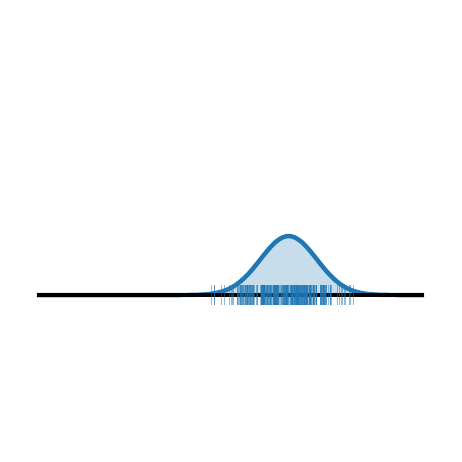
\begin{tikzpicture}
\begin{axis}[axis lines={none}, height={6.5cm}, width={6.5cm}, xmin={-3}, xmax={3}, ymin={-3}, ymax={3}, clip mode={individual}]
    \node at (-3,-3) {};
    \node at (-3,3) {};
    \node at (3,3) {};
    \node at (3,-3) {};
    \addplot[no markers, smooth, ultra thick, color={rgb,1:red,0.1216;green,0.4667;blue,0.7059}, fill={rgb,1:red,0.1216;green,0.4667;blue,0.7059}, fill opacity={0.25}]
        coordinates {
            (-3.0,-1.0)
            (-2.9,-1.0)
            (-2.8,-0.9999999999999998)
            (-2.7,-0.9999999999999986)
            (-2.6,-0.9999999999999909)
            (-2.5,-0.9999999999999438)
            (-2.4,-0.9999999999996723)
            (-2.3,-0.9999999999981868)
            (-2.2,-0.999999999990484)
            (-2.1,-0.9999999999526182)
            (-2.0,-0.9999999997761739)
            (-1.9,-0.9999999989968812)
            (-1.8,-0.9999999957348286)
            (-1.7,-0.99999998279467)
            (-1.6,-0.9999999341536179)
            (-1.5,-0.9999997609200129)
            (-1.4,-0.9999991764368138)
            (-1.3,-0.9999973085084408)
            (-1.2,-0.9999916549005841)
            (-1.1,-0.9999754522097821)
            (-1.0,-0.9999314928836516)
            (-0.9,-0.9998186150009755)
            (-0.8,-0.9995443730100476)
            (-0.7,-0.9989141748075886)
            (-0.6,-0.9975449927421185)
            (-0.5,-0.99473391284028)
            (-0.4,-0.9892831858053971)
            (-0.3,-0.9793087963610623)
            (-0.2,-0.9620992150531535)
            (-0.1,-0.9341352496846472)
            (0.0,-0.8914073851657249)
            (0.1,-0.8301404663464845)
            (0.2,-0.7479295366289559)
            (0.3,-0.6451078543883948)
            (0.4,-0.5259619407034923)
            (0.5,-0.3992795303462793)
            (0.6,-0.2777724583187935)
            (0.7,-0.17620707699520421)
            (0.8,-0.1085346586964997)
            (0.9,-0.08476363969709866)
            (1.0,-0.1085346586964997)
            (1.1,-0.17620707699520421)
            (1.2,-0.2777724583187935)
            (1.3,-0.3992795303462793)
            (1.4,-0.5259619407034923)
            (1.5,-0.6451078543883946)
            (1.6,-0.747929536628956)
            (1.7,-0.8301404663464844)
            (1.8,-0.8914073851657249)
            (1.9,-0.9341352496846472)
            (2.0,-0.9620992150531535)
            (2.1,-0.9793087963610624)
            (2.2,-0.9892831858053971)
            (2.3,-0.99473391284028)
            (2.4,-0.9975449927421185)
            (2.5,-0.9989141748075886)
            (2.6,-0.9995443730100476)
            (2.7,-0.9998186150009755)
            (2.8,-0.9999314928836516)
            (2.9,-0.9999754522097821)
            (3.0,-0.9999916549005841)
        }
        ;
    \draw[black, ultra thick] ({rel axis cs:1,0}|-{axis cs:0,-1}) -- ({rel axis cs:0,0}|-{axis cs:0,-1});
    \addplot[only marks, mark={|}, mark size={3.5pt}, color={rgb,1:red,0.1216;green,0.4667;blue,0.7059}, opacity={0.5}]
        coordinates {
            (1.029584828171896,-1)
            (1.0666825380016693,-1)
            (0.6394971710765831,-1)
            (0.895447023418512,-1)
            (0.5342766730802563,-1)
            (1.0356102884703913,-1)
            (1.9004055890657514,-1)
            (-0.0882000290702114,-1)
            (1.1310066390066154,-1)
            (1.0880522835745536,-1)
            (1.1544325438019485,-1)
            (1.3198803581543697,-1)
            (1.0999823409289662,-1)
            (0.6723186859902927,-1)
            (1.078015618822017,-1)
            (0.8780088187141819,-1)
            (0.5976433864840105,-1)
            (0.12680401057023116,-1)
            (0.9526406636981474,-1)
            (0.5697554152288482,-1)
            (0.1460167608353189,-1)
            (1.2469459607568574,-1)
            (1.192073246220382,-1)
            (1.1401109846334934,-1)
            (0.8723756556011468,-1)
            (1.4827598481127873,-1)
            (0.8681152499422684,-1)
            (0.5750596377747341,-1)
            (0.36819029891689237,-1)
            (0.8768205359630236,-1)
            (0.8280187304433074,-1)
            (-0.02206851410671773,-1)
            (0.8708965094154091,-1)
            (1.4328587659806213,-1)
            (1.1474527139706738,-1)
            (1.232801467206325,-1)
            (1.065027425741845,-1)
            (0.6185907671873769,-1)
            (0.6102874187495657,-1)
            (0.11407904602211116,-1)
            (0.33811717614057146,-1)
            (0.7538591604587681,-1)
            (0.9307161153126997,-1)
            (1.0489844491540699,-1)
            (1.6563411788632494,-1)
            (1.4666202323523352,-1)
            (0.9899520176410608,-1)
            (0.46024814056266505,-1)
            (0.5294693236711454,-1)
            (1.3922981596901058,-1)
            (0.3121878941168523,-1)
            (1.4406302695563338,-1)
            (0.8757439944207485,-1)
            (1.231010520130199,-1)
            (0.8868069699771162,-1)
            (0.7426077140987116,-1)
            (0.025036819111500463,-1)
            (0.6520400550785271,-1)
            (0.3988889798440649,-1)
            (1.7197442010199036,-1)
            (0.2589696240201562,-1)
            (0.6667069467573212,-1)
            (0.4800009251461627,-1)
            (0.2962453907117797,-1)
            (0.9585401163623082,-1)
            (0.6314409715436357,-1)
            (0.1502740211836675,-1)
            (1.0398200875657426,-1)
            (0.2691047804514879,-1)
            (0.6854239638388055,-1)
            (0.7199393838365724,-1)
            (1.3367305134447531,-1)
            (1.4120317190789868,-1)
            (0.32158703647992415,-1)
            (0.20553373948494247,-1)
            (0.7087707550144227,-1)
            (1.4343127419017703,-1)
            (1.549079403991433,-1)
            (1.8412751037900579,-1)
            (0.5035672869103921,-1)
            (1.4003232695714372,-1)
            (0.679844133616686,-1)
            (0.7835881782333155,-1)
            (1.5534348663185078,-1)
            (1.2475368261469093,-1)
            (0.8251836652999842,-1)
            (0.6955329383839233,-1)
            (0.9948601116135241,-1)
            (1.056548289667431,-1)
            (1.0394955395206757,-1)
            (1.0129897778510424,-1)
            (1.1003768343547842,-1)
            (0.9915309322945648,-1)
            (1.563936760342973,-1)
            (1.4491317366763443,-1)
            (0.8279547665167923,-1)
            (0.9680836018752585,-1)
            (0.5450481923632396,-1)
            (0.15468572832528016,-1)
            (1.5538077623570097,-1)
            (0.843806975940564,-1)
            (0.7037693561968855,-1)
            (0.22579526442898146,-1)
            (0.042715354726225785,-1)
            (1.521179815429401,-1)
            (0.7262457872234388,-1)
            (1.2772012581302006,-1)
            (0.23531724469722226,-1)
            (0.891964442492118,-1)
            (0.625474450859717,-1)
            (1.0741116005386968,-1)
            (0.7489081472103332,-1)
            (0.9574252730070444,-1)
            (1.4611405367158943,-1)
            (1.1751734805246028,-1)
            (0.36223124142358565,-1)
            (0.5257516916655526,-1)
            (1.0125755734721347,-1)
            (0.26360542041860835,-1)
            (1.1220978596908742,-1)
            (0.3569244686913795,-1)
            (0.3195456983078354,-1)
            (0.30687023786814094,-1)
            (1.1366549785422686,-1)
            (-0.2481312390134759,-1)
            (0.9653405231285416,-1)
            (0.17695631837263337,-1)
            (-0.29808721961121665,-1)
            (0.7177691580794013,-1)
            (0.2760993725755183,-1)
            (1.4030429898771897,-1)
            (0.6883630388734756,-1)
            (1.2380056079362312,-1)
            (1.2295587557354748,-1)
            (0.19092514418374695,-1)
            (0.48822161010372356,-1)
            (1.1869561995391498,-1)
            (0.7043066939158933,-1)
            (1.4165807111088022,-1)
            (1.7594094203903865,-1)
            (0.8677356654885773,-1)
            (0.8118969424595366,-1)
            (0.2644714727718115,-1)
            (1.6834432155141692,-1)
            (0.5048716362737153,-1)
            (0.4770907531441041,-1)
            (0.5648317086366266,-1)
            (0.727390516232979,-1)
            (1.107127308546585,-1)
            (1.1783733791119275,-1)
            (0.7261898840547666,-1)
            (0.8649777095528668,-1)
            (1.3366919062210385,-1)
            (0.5927653356175736,-1)
            (0.27491185890728176,-1)
            (1.08950354460642,-1)
            (0.8598084342308725,-1)
            (0.6977109573574093,-1)
            (1.8536540167470752,-1)
            (1.1524418909054648,-1)
            (0.5012809340647827,-1)
            (0.8324109779304253,-1)
            (0.9264662842813131,-1)
            (0.7819353515586007,-1)
            (0.9484024771992164,-1)
            (1.1801881360597786,-1)
            (0.42344328503681855,-1)
            (0.9378170852107978,-1)
            (0.8691481890087134,-1)
            (1.4447359220165579,-1)
            (0.965908027958606,-1)
            (1.0548097178246478,-1)
            (0.4966521206561851,-1)
            (0.798392615055012,-1)
            (1.4930765785177207,-1)
            (1.2187215459441192,-1)
            (1.1086769258936393,-1)
            (1.1637719599908158,-1)
            (1.4566194568750752,-1)
            (0.291410852454145,-1)
            (0.951042635453708,-1)
            (1.1731654556809934,-1)
            (1.0366002056792936,-1)
            (1.3298974013892617,-1)
            (1.1208255516868904,-1)
            (1.2800155926316923,-1)
            (1.2049331134228005,-1)
            (1.7759883898566633,-1)
            (0.9665598121571971,-1)
            (0.5565615076832997,-1)
            (1.335313310800165,-1)
            (0.6840644292313198,-1)
            (1.0585936645899205,-1)
            (1.1943757732922569,-1)
            (1.1619218661721789,-1)
            (0.24523372753310224,-1)
            (0.7375283009466356,-1)
            (0.34352521313924667,-1)
            (1.1811949261518027,-1)
            (1.7307557908577134,-1)
            (0.2077507002609158,-1)
            (1.029626663680191,-1)
            (1.0320233874164235,-1)
            (0.8556398765539684,-1)
            (0.6247015815448483,-1)
            (1.1719346420528685,-1)
            (0.01844258630818485,-1)
            (0.5838409446219854,-1)
            (0.47645616170586136,-1)
            (0.10761037664853879,-1)
            (1.280056399159755,-1)
            (0.16749061782694707,-1)
            (0.6653827431074919,-1)
            (0.42420190637933575,-1)
            (-0.13443506769569835,-1)
            (1.4750850616945534,-1)
            (1.0276542168944816,-1)
            (1.1910438043996137,-1)
            (0.9920254894201074,-1)
            (1.0418622004665874,-1)
            (1.0369856223548666,-1)
            (0.35792168661652013,-1)
            (1.2802892099678544,-1)
            (1.0753732878330338,-1)
            (0.4996771726988574,-1)
            (1.1462748371106515,-1)
            (0.5187964210290879,-1)
            (0.68771313571544,-1)
            (0.6695198243283164,-1)
            (1.180840822782021,-1)
            (1.2966269018756036,-1)
            (0.3059561428580503,-1)
            (1.2809614944840755,-1)
            (0.5273606248024915,-1)
            (1.229139404178201,-1)
            (0.5322752171103267,-1)
            (1.0210304992682624,-1)
            (0.506375866532563,-1)
            (0.24034562361380685,-1)
            (0.6125846816098957,-1)
            (0.5772899789960086,-1)
            (1.3948016807968122,-1)
            (0.5095542463197718,-1)
            (0.9093149534289493,-1)
            (0.22243557334542474,-1)
            (0.9844475342897381,-1)
            (1.3012998862357688,-1)
            (0.9713311815901338,-1)
            (1.0136187936640892,-1)
            (-0.24227747499702235,-1)
        }
        ;
\end{axis}
\end{tikzpicture}
\end{document}

\caption{Draw samples}
\end{subfigure}
\caption{Illustration of distributional conditioning of a bivariate Gaussian. Here, we form the joint distribution, calculate the conditional distribution, and then draw samples from it. Note that all steps except the very last one are \emph{distributional} in nature and do not involve the use of random variables, which only appear at the very end of the process.}
\label{fig:mvn-dist-cond}
\end{figure}

The non-singularity requirement is more-or-less necessary: otherwise, the marginal distribution of $\v{y}$ may admit too many null sets, rendering the desired conditional distribution non-unique, except in regions where one can apply a linear map to recover a suitable Lebesgue density and apply the above argument on the obtained subspace.

Of one wants to work with this expression numerically, then it's possible to calculate the desired conditional mean and covariance. 
In particular, one can generate conditional sample via the expression
\[
(\v\theta\given\v{y})(\omega,\v\gamma) &= \m{L}_{\v\theta\given\v{y}}\v{z}(\omega) + \v\mu_{\v\theta\given\v{y}}
&
\v{z} &\~[N](\v{0},\m{I})
\]
where $\v\mu_{\v\theta\given\v{y}}$ is the conditional mean, and $\m{L}_{\v\theta\given\v{y}}$ is a Cholesky factor of the conditional covariance.
This enables one to calculate any quantity of interest depending on the conditional distribution numerically via the Monte Carlo method.
The computational costs will be cubic in the dimension of both $\v\theta$ and $\v{y}$, owing to the need to compute $\m{L}_{\v\theta\given\v{y}}$ and invert $\m\Sigma_{\v{y}\v{y}}$, respectively.


\subsection{Pathwise conditioning}

The preceding considerations gave us closed-form analytic expressions for Gaussian conditionals in terms of matrix-vector expressions that can be computed numerically.
From this, one might be tempted to conclude that there is nothing more to say conditioning multivariate Gaussians---this, however, would be a significant mistake.
Miraculously, Gaussian conditional distributions---in general, a purely \emph{distributional} notion---can also be described in a \emph{pathwise} manner using \emph{random variables}.

\begin{restatable}[Matheron's update rule]{theorem}{thmmvnpw}
\label{thm:mvn-pw}
For $\v\theta,\v{y}$ defined in \Cref{prop:mvn-cond}, we have that
\[
(\v\theta\given\v{y})(\omega,\v\gamma) = \v\theta(\omega) + \m\Sigma_{\v\theta\v{y}}\m\Sigma_{\v{y}\v{y}}^{-1}(\v\gamma - \v{y}(\omega))
.    
\]
\end{restatable}

\begin{proof}
By direct calculation,
\[
\E(\v\theta + \m\Sigma_{\v\theta\v{y}}\m\Sigma_{\v{y}\v{y}}^{-1}(\v\gamma - \v{y})) = \v\mu_{\v\theta} + \m\Sigma_{\v\theta\v{y}}\m\Sigma_{\v{y}\v{y}}^{-1}(\v\gamma - \v\mu_{\v{y}}) = \E(\v\theta\given\v{y}=\v\gamma)
\]
and 
\[
\Cov(\v\theta + \m\Sigma_{\v\theta\v{y}}\m\Sigma_{\v{y}\v{y}}^{-1}(\v\gamma - \v{y})) &= \m\Sigma_{\v\theta\v\theta} + \m\Sigma_{\v\theta\v{y}}\m\Sigma_{\v{y}\v{y}}^{-1}  \m\Sigma_{\v{y}\v\theta} - 2\m\Sigma_{\v\theta\v{y}}\m\Sigma_{\v{y}\v{y}}^{-1} \m\Sigma_{\v{y}\v\theta}
\\
&= \m\Sigma_{\v\theta\v\theta} - \m\Sigma_{\v\theta\v{y}}\m\Sigma_{\v{y}\v{y}}^{-1}  \m\Sigma_{\v{y}\v\theta} = \Cov(\v\theta\given\v{y}=\v\gamma)
\]
where we have cancelled a factor of $\m\Sigma_{\v{y}\v{y}}\m\Sigma_{\v{y}\v{y}}^{-1}$ in the middle term.
\end{proof}

This affirms the claim, but gives few hints on where this expression originates or how to obtain it from first principles.
To better understand this, we now prove \Cref{thm:mvn-pw} in a different way.
To do so, we first prove a general result about conditioning.

\begin{lemma}
\label{lem:cond-repr}
Consider three random vectors $\v{a} : \Omega \-> \R^m$, $\v{b} : \Omega \-> \R^n$, and $\v{c} : \Omega \-> \R^m$ such that 
\[
\v{a} = f(\v{b}) + \v{c}    
\]
where $f : \R^n \-> \R^m$ is a measurable function, and where the random variables $\v{b}$ and $\v{c}$ are independent. 
Then we have 
\[
(\v{a} \given \v{b} = \v\beta) = f(\v\beta) + \v{c}    
.
\]
\end{lemma}

\begin{proof}
This follows by direct calculation by writing
\[
\int_{A_{\v{b}}} \pi_{\v{a}\given\v{b}}(A_{\v{a}}\given\v\beta) \d\pi_{\v{b}}(\v\beta) &= \P(\v{a} \in A_{\v{a}}, \v{b} \in A_{\v{b}}) 
\\
&= \P(f(\v{b}) + \v{c} \in A_{\v{a}}, \v{b} \in A_{\v{b}})
\\
&= \int_{\R^m\x\R^n} \1_{f(\v\beta) + \v\varsigma \in A_{\v{b}}, \v\beta\in A_{\v{b}}} \d(\pi_{\v{c}}\ox\pi_{\v{b}})(\v\varsigma,\v\beta)
\\
&= \int_{A_{\v{b}}} \int_{\R^m} \1_{f(\v\beta) + \v\varsigma \in A_{\v{b}}} \d\pi_{\v{c}}(\v\varsigma) \d\pi_{\v{b}}(\v\beta)
\\
&= \int_{A_{\v{b}}} \P(f(\v\beta) + \v{c} \in A_a) \d\pi_{\v{b}}(\v\beta)
\]
where we have used independence to represent the probability as an integral over a product measure, followed by Tonelli's Theorem.
By the Disintegration Theorem, $\pi_{\v{a}\given\v{b}}$ is $\pi_{\v{b}}\ae[-]$ unique, implying that the conditional distributions of interest are equal, and the claim follows.
\end{proof}

The key idea behind our argument will be to choose the \emph{conditional expectation} for our function $f$, or more precisely, the map $\v{y} \|> \E(\v\theta\given\v{y})$.
We now recall this notion and some of its key properties.

Conditional expectation is defined as the orthogonal projection from the Lebesgue space $L^2(\Omega,\c{F},\P;\R^n)$ onto the subspace $L^2(\Omega,\sigma(\v{y}),\P;\R^n)$ where $\sigma(\v{y})$ is the smallest $\sigma$-algebra containing all preimages $\v{y}^{-1}(A_{\v{y}})$ where $A_{\v{y}}\in\c{B}(\R^n)$. 
Recall that the preimage is a map $\v{y}^{-1} : \c{B}(\R^n) \-> \c{F}$ between $\sigma$-algebras.
This definition might seem daunting, but is reasonably intuitive: we can think of this as projecting onto the subspace induced by all collections of random numbers in $\Omega$ which play a role in determining what $\v{y}$ does.

Recall that $L^2(\Omega,\c{F},\P;\R^n)$ is a Hilbert space of equivalence classes of random variables with inner product given by $\innerprod{\v{a}}{\v{b}} = \E(\v{a}\cdot\v{b})$.
Using this, it follows from the Projection Theorem for Hilbert spaces that the terms\footnote{TODO: check.} $\E(\v\theta\given\v{y})$ and $(\v\theta - \E(\v\theta\given\v{y}))$ are uncorrelated---and, in the Gaussian case, that they are independent.
This gives us the candidate random variables to use for $\v{b}$ and $\v{c}$, if we choose conditional expectation for $f$.

Finally, recall that for multivariate Gaussians, we have $\E(\v\theta\given\v{y}) = \m\Sigma_{\v\theta\v{y}}\m\Sigma_{\v{y}\v{y}}^{-1}\v{y}$, where we note in our setting that the inverse always exists by non-singularity of $\v{y}$.
With these preparations, we are ready to revisit \Cref{thm:mvn-pw}.

\begin{figure}
\begin{subfigure}{0.49\textwidth}
\documentclass[tikz,11pt]{standalone}
\usepackage{lmodern}
\usepackage{pgfplots}
\pgfplotsset{compat=1.17}
\usepgfplotslibrary{external}
\usepgfplotslibrary{groupplots}
\usepgfplotslibrary{fillbetween}
\usetikzlibrary{fadings}
\begin{document}
\tikzsetnextfilename{figures/tex/mvn-pw-joint.pdf}
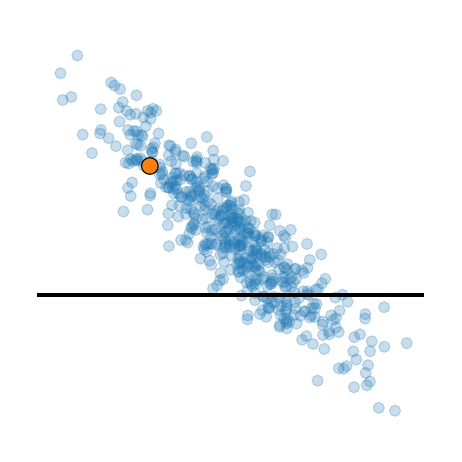
\begin{tikzpicture}
\begin{axis}[axis lines={none}, height={6.5cm}, width={6.5cm}, xmin={-3}, xmax={3}, ymin={-3}, ymax={3}, clip mode={individual}]
    \node at (-3,-3) {};
    \node at (-3,3) {};
    \node at (3,3) {};
    \node at (3,-3) {};
    \addplot[only marks, color={rgb,1:red,0.1216;green,0.4667;blue,0.7059}, opacity={0.25}]
        coordinates {
            (0.2972879845354616,-0.10087664808024613)
            (-0.5976344767282311,0.5333180524739201)
            (-0.839026854388764,0.8907344574202789)
            (2.2950878238373105,-3.053779070523791)
            (0.5299655761667461,-0.28891673497551795)
            (0.5837082875687786,-0.105457100657531)
            (0.45879095505371686,-0.6405931735580526)
            (0.40839583832475224,-0.38954743577809514)
            (-0.6936536438038856,-0.1489077100062718)
            (0.12076596493743928,-0.43893395321484724)
            (-1.7297561813906863,1.903726524008475)
            (0.6700619812560624,-0.3629447984969627)
            (-0.06337459242956062,0.6397969812993919)
            (-0.07314863333773934,-0.25910659222130056)
            (-1.2200551285346526,1.074870151644211)
            (-0.1651363578028337,-0.7734457920841674)
            (-0.0667679865065892,0.5929499538365516)
            (0.5676954597384435,-0.1781244465582743)
            (0.37859887985335006,-0.6221482246806381)
            (-0.6646462443910314,-0.18773933402596066)
            (-1.2890476038497443,1.0140020039235378)
            (0.07046760136115796,0.08556360792902756)
            (1.7351656660543822,-0.9950288670966089)
            (0.20636408140261675,-0.62547953269969)
            (-0.8500556703153979,1.257348262973964)
            (-1.348533456491827,1.754310380398978)
            (-0.055647093207324264,0.38109290401679086)
            (-0.030266886646762546,-0.13015208791920213)
            (-2.0073032025325626,1.5586129373578335)
            (-1.1496275243969976,1.8544089729772013)
            (-1.4706245413873802,1.0902690340059635)
            (-0.9635439598255011,0.26343495455473065)
            (0.13430023756127,-0.3894292422615074)
            (-1.719989356319742,1.6878105082535104)
            (-1.4473728978815112,1.0880595719321655)
            (-0.4130873839831828,0.8085091590296176)
            (1.174681325975111,-1.6356261568976758)
            (-1.593214868044067,1.2426641362540831)
            (1.225797497997867,-0.4541383442066472)
            (2.1594331871008534,-2.3399225814803764)
            (1.1478203006125018,-1.2531941369345656)
            (-0.2670670352181297,0.8937951980148244)
            (0.7973041601753904,-0.792390078857867)
            (-0.46907960993009634,0.5170317605506107)
            (0.35914640760234967,-0.18373622732143902)
            (0.2592163280556861,-0.032917860895333384)
            (0.20998636004214272,0.4749490363050444)
            (1.2597946036121963,-1.2058603767341844)
            (0.15619449488763584,-0.4955268530356326)
            (-1.7098682060045913,2.192689147761142)
            (-0.1289156385300165,-0.08020656912609962)
            (-1.546731741900333,0.5347739224365254)
            (1.4250842322231618,-1.456330021777407)
            (0.865359034508392,-1.4435058863603305)
            (-0.018434833227298542,-0.2579341992357144)
            (0.3994394061296323,-0.5105873183063359)
            (0.13174261149628444,0.44257218636923823)
            (0.6312912597626849,-1.1059308923628306)
            (-0.8585845030636355,0.8853016262294067)
            (-1.4599892950591262,1.5360882252440877)
            (-1.2459007156231243,0.5408563423686472)
            (-1.360732996599522,1.4613146754818385)
            (-2.63399370777994,2.4359348601304873)
            (-1.6587759684101517,0.29481115195791996)
            (-0.4180662233306449,-0.24764102642690128)
            (1.1540597669111703,-1.2502907513465775)
            (0.7754380459705584,-0.36833548563802787)
            (-1.626729284162485,1.0522779658499601)
            (0.658322671059814,-0.7881837100379394)
            (1.1851174294240252,-0.2071962660912362)
            (-0.0740194597978335,-0.021485543722413278)
            (-1.458002434697322,2.0956454067417587)
            (-0.9064866353733989,0.39292872498016307)
            (-0.7689287953327062,0.5194264320324146)
            (0.4751826349484905,-0.14929099234171395)
            (-0.3987477530370317,0.32385068728619537)
            (1.0018399414103412,-1.2088906116517335)
            (-1.4340505462257125,1.4801490362095613)
            (-0.09220577556331351,-0.11930384463560857)
            (2.187832361106393,-1.7166072340902891)
            (-0.9147242711971281,0.7556628220078405)
            (0.060717820312243403,-0.17271068672241838)
            (0.11104289827811374,0.18024952760947624)
            (-1.0932960849422242,1.0217835616587996)
            (-0.07077890859801883,0.6084369397547749)
            (0.1512033860208509,0.018726670405881995)
            (-0.9253434974479612,0.731201762758177)
            (1.3606109850208474,-0.9058283405746437)
            (0.4787377009574211,-0.1670919708708632)
            (1.276972611856289,-1.7578644982165152)
            (0.11709983671299977,0.1677756026392937)
            (0.3133823643278484,0.14785327349419808)
            (0.5066085599761962,-0.07593211134688438)
            (0.6995645399732705,0.24638030388071974)
            (0.15269868152330113,-0.4808673056876713)
            (0.9986772266084378,-1.1147450747162742)
            (0.3638388194911837,-0.033079164249808446)
            (0.6008899714463747,-1.195567246768635)
            (-0.3727356407152467,-0.22101271021703134)
            (0.6451054034379425,0.250160927763565)
            (-1.5881288112102452,1.5589425937694117)
            (0.3028824231221631,-0.3169543042559784)
            (-0.6315778870329364,0.8403547403825111)
            (-2.0224314101114222,1.5040292137222653)
            (-0.9716762048860438,0.08211896104597816)
            (0.8719091772543835,-1.5172276417019983)
            (-0.5382489016869288,0.008625917897571722)
            (-2.373156801968529,2.7109261834662295)
            (0.2928588585051935,0.02747083174493936)
            (0.21112095190111557,-0.04814665624441669)
            (0.3142665708225735,-0.824918227123796)
            (0.8724432818783148,-0.6098256658574496)
            (-0.918403552104298,1.0728380340045198)
            (-0.8745409882369648,0.5748000251287083)
            (-0.5287577864433531,0.756722830581039)
            (0.909924517665989,-1.41297592304134)
            (0.8739856083349014,-1.1592264226989197)
            (0.7550975795526141,-1.047312604487026)
            (0.27766300810348893,-0.6435208407605771)
            (-1.513350928595663,1.0746005173459925)
            (-0.7403475629601508,1.161114487460948)
            (-0.8957439911719416,0.8154845454836968)
            (-1.5544394018554584,1.4834429959596507)
            (0.9206450790295183,-0.7572493895364327)
            (0.2606593892993496,-1.376870925366437)
            (-1.0562153109753674,0.9112105616016073)
            (0.27865272355818926,-0.27954244300337383)
            (-0.1569479584427068,-0.6603783867108125)
            (-0.5674519382746356,0.11002863000303026)
            (-3.8819978594268876,3.8715166318421317)
            (0.432306709021104,-0.5298667000323366)
            (0.3402161710448687,-0.4367949598488905)
            (1.9136035721789713,-2.42799190804498)
            (0.5169712744781768,-1.0243382924896245)
            (1.0840840119878734,-1.3219551464549286)
            (-0.025668064894330093,0.018104867554613876)
            (1.4678868411216563,-0.7475344564343945)
            (0.27236940715678176,-0.052305515584656515)
            (-1.1966483101519632,1.2882069773574079)
            (1.4147590837932418,-0.8177050497305656)
            (-0.1978660512585745,0.32145282082298665)
            (-1.7983067508193347,2.2463755315612124)
            (-0.5232908450257276,0.6605313698453924)
            (0.07774415899993356,-0.007529835312156244)
            (-0.43422769970595093,0.49710846972113587)
            (-0.12389276233418343,0.2984527837168319)
            (1.189248289168407,-0.9805534479118881)
            (1.0218854109275881,-1.4423571264238406)
            (2.3805130457880845,-1.188033443784486)
            (2.1299921566412503,-2.085970102894445)
            (-0.23211025519653547,0.29881002254612327)
            (1.107610369079468,-0.6190411563111236)
            (1.6776251628069427,-2.133117254191005)
            (-1.3830239105437792,1.477600144441786)
            (0.27246958339005234,0.27523273174208196)
            (0.6546787209966946,-0.7421339359792656)
            (-3.2998673372242706,2.4329415466777466)
            (0.5439858444482804,-0.455308019368296)
            (-1.8487276149711611,2.2922382967671315)
            (-0.10777043967832316,-0.26447033241910123)
            (-2.1473888794968143,1.1989359932661814)
            (-1.3931348022399552,1.1196084377040847)
            (0.8249874857828697,-0.07914426711418421)
            (-0.7164282891787297,0.8537985786816389)
            (-1.4667181528682052,1.8082132347320654)
            (0.8156139596767987,-0.7310011388445395)
            (-0.5908786155028164,0.8010190136191977)
            (-1.0802915526773837,0.7334208710621327)
            (-0.5775086066033142,1.0660012496529352)
            (0.6635670227160482,-1.026025748737541)
            (0.3786665366937789,-0.5634799820300157)
            (0.2624053715987166,-0.9380903867743564)
            (-1.774970345560557,1.306970598477777)
            (1.9168347916309745,-1.6512853829357856)
            (-0.7629697960098806,0.519096125677645)
            (-0.19755430324781426,0.6564511543726108)
            (0.15137376741018294,-0.14590883137280247)
            (0.8448917445918529,-0.7125551091022019)
            (-0.5595352207192429,0.24226993625911364)
            (1.633608902780053,-1.3568888711086873)
            (0.9401341655808859,-0.8759797406628419)
            (-0.001285241025904152,-0.16681927145477513)
            (0.04414459834517204,0.1977061652106734)
            (-0.36690604870636645,-0.03950040691101725)
            (0.7209794667689048,-0.2720741629778893)
            (0.3536205284606749,-0.5494390717986374)
            (-0.5293369148430024,1.069815877530889)
            (-0.7940239797611804,0.38289998576785605)
            (-0.9540680773126435,-0.24139761982770558)
            (-0.11409699214027211,-0.7515973911431816)
            (-0.393771885226301,1.0479161238455657)
            (0.26835044888970766,-1.3153914225138363)
            (1.5310536307073936,-1.6059775212726701)
            (0.5834052352999808,-0.4940769489651093)
            (-0.6101715120745413,1.3519805785953578)
            (-0.2805179483106536,0.2579073363572935)
            (0.131810280826272,0.32274053423714155)
            (-0.17667143438293495,0.18265907962212377)
            (0.8325802393139106,-0.2751839789726437)
            (-0.5993789779066115,0.027342200479943735)
            (0.16820569915460176,-1.0085515999241068)
            (0.13120625565482671,0.11975436757503295)
            (0.8698862875353852,-1.1016873222639396)
            (-0.029032421388993576,0.3927881400528105)
            (-0.15393921542968417,0.22461126696996186)
            (0.08721657095184755,0.017521334567634453)
            (-0.06667541333469505,0.34542461644404543)
            (1.4334553034866289,-1.618302733519816)
            (-0.11640702062324493,1.079978295913763)
            (-0.24234887761151688,0.24857525734027514)
            (0.7338834687716466,-0.45848686850115805)
            (-0.3537417603088734,0.6117848490154096)
            (-0.3673488735340369,1.4499001176426503)
            (2.3829332688009828,-1.8011477753527503)
            (0.03131929472379513,0.1487019051192954)
            (-0.9579189021380435,1.1655608420359491)
            (0.6274414959863405,-0.826801156755987)
            (-0.29438920541698516,-0.200918090551567)
            (-1.590717875491105,0.6580481529553509)
            (-1.2289146699114444,1.2627103366824262)
            (0.3914757161202707,-0.8272802027459634)
            (1.6896534499381899,-1.241659010120253)
            (-0.611968992291528,0.793946425577545)
            (0.3740840174093429,0.12267077653416325)
            (0.5808485859606817,-1.1829178552331354)
            (-1.5457001328588873,1.1048227019238768)
            (1.75361653512699,-2.141628353274176)
            (-0.531704625724874,0.1922036314355785)
            (-1.4980375731640485,1.5411885401438887)
            (0.5852478579163195,-0.10032099522446003)
            (-0.6877739300923975,0.59851727586995)
            (0.9966182023827315,-0.5954799621209282)
            (0.9599688052642058,-0.24886990064144054)
            (-0.40406029223492207,0.5491396778484607)
            (2.297379718927148,-2.747884960531122)
            (-1.3942524420044087,1.3121107080076224)
            (1.30993212700943,-1.2054498085495136)
            (0.746144255590275,-1.2261354102499837)
            (1.9487894951751723,-1.9989987359284322)
            (-0.6132329004972873,0.5591516786366368)
            (2.084230975839466,-1.3644751544267126)
            (0.38407455255519346,-0.3575657703398731)
            (-1.5785427534891785,1.0368323514483362)
            (1.8128382404129062,-1.1032328963834872)
            (-1.2123395817818958,1.2143991979887445)
            (0.2083343858982014,0.11785096365280404)
            (1.4046974354664667,-0.3700884195731384)
            (0.34013510486070253,-0.8585151885806933)
            (-1.2390463290112987,1.7286347285810262)
            (-0.8565863624820894,0.6856724400310634)
            (0.4538012969765639,-1.2950391361408786)
            (-0.9991007427732405,0.6724692092684246)
            (0.4662463238027101,-0.11655524693662578)
            (-0.792486173126059,0.8889859149331651)
            (0.1422610288642994,0.04166996146333768)
            (0.5165798439917115,-0.7175689095522795)
            (0.572932361603122,-1.0565363708688371)
            (0.1566513785833087,-0.7260310725566597)
            (0.23826183544768417,-0.43088636042927625)
            (1.193523304759714,-0.9433041331298971)
            (0.4091271950968771,-0.7560125520346963)
            (-0.32605180937465755,-0.4666031522072205)
            (-0.528112745560178,1.0969320628151762)
            (-1.0884645271492055,0.9753804876900225)
            (-0.8554296175519289,1.2188976352376453)
            (1.675948808787312,-1.574676993393196)
            (0.2666602308412965,-0.53143805527337)
            (-0.3688296792504201,0.20057296390434767)
            (0.06677792368156305,-0.2818814739091185)
            (-0.3523456900970411,0.44294736054753836)
            (-0.2405766371227846,-0.21836725104754706)
            (-0.3622644857512414,0.7616261111933353)
            (-1.2857410076345577,0.32351632878333625)
            (0.825156200939433,-0.8020049703309314)
            (1.7992548094594971,-2.1007188454222834)
            (0.10848097145565462,0.2719652356610049)
            (0.5949706804435368,-0.3489523943888211)
            (1.1079660978130559,-1.6929800308297969)
            (0.25989707779870364,-0.030648122518285303)
            (-0.3919576066101382,-0.2090688267826724)
            (-0.08111315760776971,-0.21741634978159619)
            (-0.630814741681354,0.8490910651791808)
            (1.13580872262362,-0.6569536540548457)
            (-0.0799246177593996,-0.18092074377431283)
            (-0.4387702731149963,0.17508014174444658)
            (0.0012495783650486236,-0.6069923524705545)
            (-0.4821758306182083,0.6013390644723547)
            (0.3126572456108897,-0.4289690059668188)
            (0.17824576718381163,-0.15713391453230402)
            (-0.03222208961967493,0.045146912348522014)
            (-1.525082270589168,0.7445062424975258)
            (-0.08789055046010402,-0.02513131951625694)
            (-1.3426658027254874,1.004408990932128)
            (-1.2401064426390593,0.5762565389382952)
            (0.1766983746369227,-0.6035758949232014)
            (0.8305441585121899,-1.3690803554375794)
            (-1.062426745485554,0.877465212758632)
            (-0.7792124017891849,0.7889399427741401)
            (-0.39607292077168643,0.8409048697721295)
            (-0.2687142882698926,1.2382128234154328)
            (-0.00119442020718918,0.3815958468627311)
            (1.3221375148350687,-0.9132684464335817)
            (-0.9611868737662628,0.6644334474884017)
            (0.9476400830565346,-0.7131257480218709)
            (0.4982972465694152,-1.0225669466212737)
            (0.1431480547985834,-0.29834175355580383)
            (-0.01653802057118619,-0.22275574923341357)
            (0.13323968501086753,-0.12938097895609246)
            (1.6326868249717172,-1.501554762860129)
            (0.009275324748154191,0.4261866431900248)
            (1.4319586745069863,-1.4102185712646864)
            (0.18314474353215668,-0.19438278991957553)
            (-1.612809018801593,1.8536949892686776)
            (1.29069196187616,-1.1368480152314493)
            (3.124318593443059,-3.2531886837614876)
            (-0.28715298455425015,0.9329817064205438)
            (-0.11556009086388684,-0.3507826440767556)
            (0.30077062196830734,0.914227110215188)
            (0.017529407674652085,0.4489838819899084)
            (-0.8089189600547338,0.21562178213204575)
            (-1.1710373555532807,1.351871086200737)
            (-0.7665852772824016,-0.14652733242349747)
            (0.11702518739433772,-0.6416873744306543)
            (1.0102928065517993,-0.5918397818918703)
            (1.9016982514072045,-1.8723224317422273)
            (-2.2895905972982606,1.4867380417532492)
            (2.5483208898247103,-2.791926964790314)
            (-1.365734006824005,1.0721329392212648)
            (-1.2367794349539312,1.8287278679932657)
            (0.7612395595485809,-1.4930083770916784)
            (1.5909826424480042,-1.3873394516726332)
            (0.8545444889487256,-1.2564957593207051)
            (-0.6367201621923837,0.45192057065970526)
            (0.988027300039114,-0.95824234844789)
            (0.3885790331353395,-0.08030636590725965)
            (-0.2614930295213064,1.099332727685738)
            (1.1932460546819013,-0.5769588061590163)
            (0.843689267655445,-1.062541317581636)
            (0.17404214583167332,-0.2227029745734701)
            (0.9331744539977493,0.010756726433466923)
            (0.15991438966878682,0.13971827764498546)
            (-0.11390296246278847,0.11219094460796383)
            (1.6254676981101484,-1.0382911566135475)
            (0.2628347548441931,-0.5627104759959763)
            (0.3513428690933362,-0.31512388586110723)
            (-0.6949663889620127,0.256576558860079)
            (-0.10884891545390497,0.7031555956921597)
            (2.729445820551839,-1.7458795930669253)
            (-0.36792522369791164,-0.3270176758895879)
            (-0.05528883473746865,0.13070422921872524)
            (-0.3339535425294759,-0.20661633831096599)
            (-0.5720644165807692,0.08638819724675634)
            (0.9822822445625023,-1.3098499689416847)
            (0.008154305444488837,0.17862785276080292)
            (0.37847076773415456,-1.0794003857716605)
            (-1.5531425959603435,1.793555441359969)
            (-1.2008763348459806,1.8861374274951346)
            (0.8379852615245372,-0.5713165764500935)
            (0.861525601405543,-0.8663091825668433)
            (-0.6624402142053086,0.4840225450502453)
            (2.094064358256568,-2.2054002029076734)
            (2.110576071498333,-2.397038788668987)
            (-0.21345648146548854,-0.2179959280815545)
            (0.6341198754901243,-0.7954371454868959)
            (0.6183000885232028,-0.8317625276625111)
            (-0.3091091627491842,0.9655192645873627)
            (-0.6815274819963835,0.346169784313342)
            (0.605999681311456,0.08051940055855189)
            (0.37619020514195034,-0.7971288514199739)
            (2.006165198118277,-1.6089884039003837)
            (-0.09982010028904506,-0.49023091987671963)
            (0.7638568575849538,-1.466578433623644)
            (0.3813870602943384,-0.9707439455834941)
            (-0.4088361702003478,-0.29326846874825335)
            (-0.520893143837836,0.6913758657094472)
            (-1.8898609632139673,1.4300757043367518)
            (0.30423375743841535,-0.46608275281434836)
            (0.8658098173642257,-1.2161642694291004)
            (0.31016224941683607,-0.7796798943093933)
            (0.782603001925965,-1.1693269362450032)
            (0.25032695818751377,-0.8058153926409749)
            (0.4707150121846368,-0.3534157937665088)
            (0.3923682520698269,-0.2638459560841252)
            (-2.0115667870090204,1.8811352161843016)
            (-0.8042222347395631,0.56886617179731)
            (-0.2895644050953529,0.8728501706922185)
            (-0.9560332307222564,0.6695465744839425)
            (-0.8694008603311896,0.7639064721703516)
            (0.8498592837097624,-0.11126015444974902)
            (-0.5184225058688992,1.1400616484531596)
            (0.6921663616623136,-0.4935800557806683)
            (0.6394740649295387,-0.6900115504415675)
            (0.55173629984778,-0.40789593571483923)
            (0.41052460590863105,-0.3193155693826418)
            (1.1274930637855678,-0.9403360898186511)
            (0.9746272376437478,-0.7977901419516686)
            (0.2718102677901078,0.03871248153621884)
            (0.5264904831050543,-0.4120638114084491)
            (-0.6085163875132199,0.054422712166160514)
            (0.3881780115667518,-0.07883848551640443)
            (-0.2535150437627753,0.9585987771793687)
            (0.6098239355865941,-0.4066558704215472)
            (-1.2821660632229595,1.8556326043232019)
            (-1.4507878031322263,1.1166069407343293)
            (0.12912659446021338,-0.24183971473231886)
            (-1.2132705181272156,1.2130290331673879)
            (-0.6417207530049402,-0.049623369119604965)
            (-0.39188919597096245,0.38111258647940705)
            (1.013630663300725,-0.7527935726315519)
            (-0.7156034341569465,1.146395116604524)
            (0.13277193762814965,-0.6343703576898402)
            (1.3084072697295053,-1.3399869816949301)
            (0.8817160139297816,-0.5229296348275051)
            (0.8462905517316545,-0.8813197451171236)
            (-0.5734932337841947,0.27931315180062166)
            (-0.20594816627575477,-0.8526678501707842)
            (-0.952539183118715,1.3209982076579012)
            (0.23745788510368965,0.6914320765870984)
            (0.8362686215120259,-0.5753258626258574)
            (-0.1973537715836528,0.49914054245865724)
            (0.47914911804336535,-0.3772305718350854)
            (-0.27097044634740913,-0.9013828933023016)
            (-0.4987134771226696,0.484510700795029)
            (0.06271981803961879,-0.2093436182957782)
            (0.14891084177869107,-0.2306471559660138)
            (0.13105150326944962,-0.5082799069312333)
            (-2.5991778979112783,2.0226988744915118)
            (2.1619447876295617,-1.8710714173102687)
            (-0.6169282510157554,0.3321726891751764)
            (1.5600696986005596,-1.3134412873715504)
            (1.0577653016664748,-1.0478741179021815)
            (1.3308298996034031,-1.136160788553338)
            (-0.08541243409544698,0.11578820322691277)
            (0.4798881756377317,-0.7542036412810156)
            (-0.6357559693783907,0.6051696574941969)
            (1.4528570085121595,-1.834090975630855)
            (-0.2017657745270218,0.14837003558261336)
            (-0.30420165880389033,0.4067494198257332)
            (-0.47935690712903745,0.6742048242630732)
            (-1.6704355359969572,1.9914560968495558)
            (-0.23832634399885072,0.016437442091930154)
            (2.0885797666683175,-1.2950808749289)
            (0.145300189379367,0.25886538427676253)
            (-1.3131044327888775,1.6174515426647527)
            (0.23056657738571848,0.15320437333166256)
            (1.206138074723419,-0.9985223373862178)
            (0.7524745980334822,-0.6028793633072561)
            (0.7747631777217553,-1.3089771267896957)
            (-0.1947163932289525,-0.04023368293830598)
            (0.5686100438844073,-0.8603654160508003)
            (-0.4645439789555292,-0.43510978637133413)
            (-0.8455950022805849,1.032823711840685)
            (-0.6198129946090122,0.5180286942432893)
            (-0.15650077346438604,-0.3760507597175722)
            (1.5222693788439343,-1.5613196325989)
            (0.016905575882719334,0.25231239212669965)
            (0.15794114157783035,-0.23915597396669433)
            (0.029460520662888217,0.19952264679295453)
            (-0.2752430528657675,0.6883153182125488)
            (-0.4899845943580537,0.6277581694759209)
            (-0.8897003928635907,0.6493929310150566)
            (-0.07057372416300674,0.6559314906853326)
            (-0.27622709748591684,0.9447252872157299)
            (-0.02589203734328707,0.22749615854937896)
            (0.014107858528196642,-0.3862078525727601)
            (0.7638724713652006,-0.00504691536855284)
            (0.8777645087081587,-1.3622243720095488)
            (0.5921680001678374,-1.2094684820064994)
            (-0.46109376892663934,0.3744135665761759)
            (-0.2983667089832168,-0.5337123079749361)
            (0.024444037082591914,0.3364813889887376)
            (0.09647199311730181,-0.530253674189608)
            (0.5537559149189224,-1.3373058746549003)
            (-0.9292491097153828,1.3091312807212054)
            (-0.8281572256683849,0.7808240729197009)
            (1.2500887111451808,-1.3150681644457753)
            (-1.115358345689973,1.5047745584235241)
            (-0.11218131888371889,0.34270239443096195)
            (-1.4689516268529221,1.346964451594471)
            (-2.4672625339100787,2.0677601047059855)
            (0.2017723856403366,-0.4974935754141837)
            (-1.0311499857140385,0.7917524502010079)
            (0.3864667195035178,-0.2998286906642168)
            (-0.30104605072331786,-0.10094434630034199)
            (-0.5252212129415537,0.8893059816997332)
            (-0.3903306666319088,0.04487490037307412)
            (0.6792987899414228,-1.1176655051202107)
            (1.3496566119320768,-2.3260657319766023)
            (-1.0957880343275386,0.8671804205538843)
            (-1.437126476092288,1.3297747318091493)
            (0.008118961285724492,0.12444156012610535)
            (-0.34795177426021257,0.05809488267301427)
            (-0.8420643387435566,0.6397315482464317)
            (-0.5218538031190414,1.0513466866593029)
            (1.2317603651621327,-1.3467368859995632)
            (0.8609602079684947,-1.4123970885159913)
            (0.43274606567675294,-0.6117663413170717)
            (0.4921791438493273,-1.2349595151060446)
            (-0.13891838481322696,0.2314578675312688)
            (-0.2858725217271917,0.0018888896974441072)
        }
        ;
    \draw[black, ultra thick] ({rel axis cs:1,0}|-{axis cs:0,-1}) -- ({rel axis cs:0,0}|-{axis cs:0,-1});
    \addplot[only marks, mark size={3pt}, fill={rgb,1:red,1.0;green,0.498;blue,0.0549}]
        coordinates {
            (-1.25,1.0)
        }
        ;
\end{axis}
\end{tikzpicture}
\end{document}

\caption{Sample jointly}
\end{subfigure}
\begin{subfigure}{0.49\textwidth}
\documentclass[tikz,11pt]{standalone}
\usepackage{lmodern}
\usepackage{pgfplots}
\pgfplotsset{compat=1.17}
\usepgfplotslibrary{external}
\usepgfplotslibrary{groupplots}
\usepgfplotslibrary{fillbetween}
\usetikzlibrary{fadings}
\begin{document}
\tikzsetnextfilename{mvn-pw-cond}
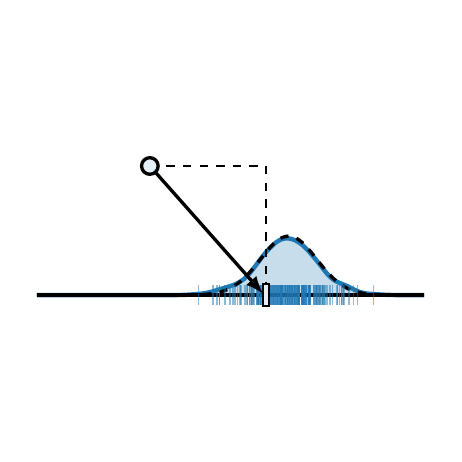
\begin{tikzpicture}
\begin{axis}[axis lines={none}, height={6.5cm}, width={6.5cm}, xmin={-3}, xmax={3}, ymin={-3}, ymax={3}, clip mode={individual}]
    \node at (-3,-3) {};
    \node at (-3,3) {};
    \node at (3,3) {};
    \node at (3,-3) {};
    \addplot[no markers, smooth, ultra thick, color={rgb,1:red,0.1216;green,0.4667;blue,0.7059}, fill={rgb,1:red,0.1216;green,0.4667;blue,0.7059}, fill opacity={0.25}]
        coordinates {
            (-3.0,-0.9999996652020177)
            (-2.9,-1.0)
            (-2.8,-0.9999997473907613)
            (-2.7,-1.0)
            (-2.6,-0.9999998060302603)
            (-2.5,-1.0)
            (-2.4,-0.9999998489954379)
            (-2.3,-1.0)
            (-2.2,-0.9999998807819237)
            (-2.1,-1.0)
            (-2.0,-0.9999999036470928)
            (-1.9,-1.0)
            (-1.8,-0.9999999180628167)
            (-1.7,-1.0)
            (-1.6,-0.9999999225693723)
            (-1.5,-1.0)
            (-1.4,-0.9999999130507876)
            (-1.3,-1.0)
            (-1.2,-0.9999998785779327)
            (-1.1,-0.9999999618301265)
            (-1.0,-0.9999944363879862)
            (-0.9,-0.9999142474709689)
            (-0.8,-0.9992536493389257)
            (-0.7,-0.9964406151579576)
            (-0.6,-0.9902743273667755)
            (-0.5,-0.9824809116853117)
            (-0.4,-0.9714896880297803)
            (-0.3,-0.9500858698006442)
            (-0.2,-0.920171598748008)
            (-0.1,-0.8903080030605133)
            (0.0,-0.8596961735320843)
            (0.1,-0.8199558592828701)
            (0.2,-0.7571852737708227)
            (0.3,-0.657805397218492)
            (0.4,-0.5287583937683515)
            (0.5,-0.3959436960884075)
            (0.6,-0.2797255759077598)
            (0.7,-0.1877676298750478)
            (0.8,-0.13140858131324085)
            (0.9,-0.12131699338214974)
            (1.0,-0.15060407874217652)
            (1.1,-0.21301846411873804)
            (1.2,-0.3088372996533647)
            (1.3,-0.42422623669650295)
            (1.4,-0.5481297047661384)
            (1.5,-0.6735010956245199)
            (1.6,-0.7669047145878339)
            (1.7,-0.8165942042654252)
            (1.8,-0.8577117016755756)
            (1.9,-0.9078233449822264)
            (2.0,-0.9509682221802819)
            (2.1,-0.9743203974646967)
            (2.2,-0.9833785516480927)
            (2.3,-0.9896665699440512)
            (2.4,-0.9956402920436492)
            (2.5,-0.9988841565223477)
            (2.6,-0.999830750301803)
            (2.7,-0.999983959600127)
            (2.8,-0.9999997103405273)
            (2.9,-0.9999995213621055)
            (3.0,-1.0)
        }
        ;
    \addplot[no markers, smooth, black, very thick, dashed]
        coordinates {
            (-3.0,-1.0)
            (-2.9,-1.0)
            (-2.8,-0.9999999999999998)
            (-2.7,-0.9999999999999986)
            (-2.6,-0.9999999999999909)
            (-2.5,-0.9999999999999438)
            (-2.4,-0.9999999999996723)
            (-2.3,-0.9999999999981868)
            (-2.2,-0.999999999990484)
            (-2.1,-0.9999999999526182)
            (-2.0,-0.9999999997761739)
            (-1.9,-0.9999999989968812)
            (-1.8,-0.9999999957348286)
            (-1.7,-0.99999998279467)
            (-1.6,-0.9999999341536179)
            (-1.5,-0.9999997609200129)
            (-1.4,-0.9999991764368138)
            (-1.3,-0.9999973085084408)
            (-1.2,-0.9999916549005841)
            (-1.1,-0.9999754522097821)
            (-1.0,-0.9999314928836516)
            (-0.9,-0.9998186150009755)
            (-0.8,-0.9995443730100476)
            (-0.7,-0.9989141748075886)
            (-0.6,-0.9975449927421185)
            (-0.5,-0.99473391284028)
            (-0.4,-0.9892831858053971)
            (-0.3,-0.9793087963610623)
            (-0.2,-0.9620992150531535)
            (-0.1,-0.9341352496846472)
            (0.0,-0.8914073851657249)
            (0.1,-0.8301404663464845)
            (0.2,-0.7479295366289559)
            (0.3,-0.6451078543883948)
            (0.4,-0.5259619407034923)
            (0.5,-0.3992795303462793)
            (0.6,-0.2777724583187935)
            (0.7,-0.17620707699520421)
            (0.8,-0.1085346586964997)
            (0.9,-0.08476363969709866)
            (1.0,-0.1085346586964997)
            (1.1,-0.17620707699520421)
            (1.2,-0.2777724583187935)
            (1.3,-0.3992795303462793)
            (1.4,-0.5259619407034923)
            (1.5,-0.6451078543883946)
            (1.6,-0.747929536628956)
            (1.7,-0.8301404663464844)
            (1.8,-0.8914073851657249)
            (1.9,-0.9341352496846472)
            (2.0,-0.9620992150531535)
            (2.1,-0.9793087963610624)
            (2.2,-0.9892831858053971)
            (2.3,-0.99473391284028)
            (2.4,-0.9975449927421185)
            (2.5,-0.9989141748075886)
            (2.6,-0.9995443730100476)
            (2.7,-0.9998186150009755)
            (2.8,-0.9999314928836516)
            (2.9,-0.9999754522097821)
            (3.0,-0.9999916549005841)
        }
        ;
    \draw[black, ultra thick] ({rel axis cs:1,0}|-{axis cs:0,-1}) -- ({rel axis cs:0,0}|-{axis cs:0,-1});
    \addplot[only marks, mark={|}, mark size={3.5pt}, color={rgb,1:red,0.1216;green,0.4667;blue,0.7059}, opacity={0.5}]
        coordinates {
            (1.10649900126324,-1)
            (0.782351770498297,-1)
            (0.8626341572894871,-1)
            (0.44668666036589877,-1)
            (1.16994051468878,-1)
            (1.3887968969770008,-1)
            (0.7822570988514695,-1)
            (0.9578031461244666,-1)
            (0.07232941719046981,-1)
            (0.6257254070440768,-1)
            (0.8835976902169411,-1)
            (1.2434116626087959,-1)
            (1.4124426907398924,-1)
            (0.5936554336630903,-1)
            (0.6473280079451371,-1)
            (0.03876242932141563,-1)
            (1.3668869719463073,-1)
            (1.3073834578359966,-1)
            (0.7186654776407757,-1)
            (0.06638835498560403,-1)
            (0.5235541996814397,-1)
            (1.047474848497283,-1)
            (1.739639685667434,-1)
            (0.5434325019728957,-1)
            (1.1815577663611696,-1)
            (1.1303458858672533,-1)
            (1.1873365204077877,-1)
            (0.7525962342259555,-1)
            (0.29544844108948753,-1)
            (1.4193405512824837,-1)
            (0.4106175892179871,-1)
            (0.17354749927375646,-1)
            (0.6838139195259134,-1)
            (0.6990401011084175,-1)
            (0.4318807168574377,-1)
            (1.2145708591434732,-1)
            (0.6026177847672027,-1)
            (0.4251828545846079,-1)
            (1.7170729882118845,-1)
            (0.9535028637685146,-1)
            (0.9199455773713928,-1)
            (1.4373486429952123,-1)
            (0.9841530892033101,-1)
            (0.8962489745654533,-1)
            (1.0937838030130547,-1)
            (1.129590253249886,-1)
            (1.5374404927166827,-1)
            (1.0745202645514302,-1)
            (0.6102203271555665,-1)
            (1.1635520269804367,-1)
            (0.6988984492564939,-1)
            (-0.16543521170746023,-1)
            (1.0143872126234956,-1)
            (0.46620373678409455,-1)
            (0.6494243874605584,-1)
            (0.83991081965393,-1)
            (1.430057579228599,-1)
            (0.5359534566361374,-1)
            (0.8381869605428306,-1)
            (0.8224901076605526,-1)
            (0.14086999250865828,-1)
            (0.8544502113341323,-1)
            (0.4583476663374988,-1)
            (-0.49344593164802375,-1)
            (0.2590568528851439,-1)
            (0.9287980906992506,-1)
            (1.3439361088963335,-1)
            (0.22032088510247916,-1)
            (0.8489573320256686,-1)
            (1.8986407899419127,-1)
            (0.8066435508519946,-1)
            (1.3280784313702612,-1)
            (0.3471492171087478,-1)
            (0.5985549934964669,-1)
            (1.240820741840948,-1)
            (0.7927178655205441,-1)
            (0.813838390923781,-1)
            (0.7980835863628928,-1)
            (0.7004207642646387,-1)
            (1.5428858504251326,-1)
            (0.6653722686099285,-1)
            (0.8052782022620668,-1)
            (1.1732674731266424,-1)
            (0.7263091205506955,-1)
            (1.3768143371812787,-1)
            (1.0680573893861447,-1)
            (0.6327380890343982,-1)
            (1.445365478503668,-1)
            (1.2283549271736443,-1)
            (0.5948945634614252,-1)
            (1.1680978790883643,-1)
            (1.3464503104726266,-1)
            (1.3382696597640003,-1)
            (1.8213068134659185,-1)
            (0.6199181064043969,-1)
            (0.895406659363791,-1)
            (1.234067571666356,-1)
            (0.42487944935460326,-1)
            (0.32835292008942507,-1)
            (1.770250238425151,-1)
            (0.7149195231822254,-1)
            (0.9176235492917826,-1)
            (1.0247413793113238,-1)
            (0.23119488223861673,-1)
            (0.002230860055336681,-1)
            (0.40640429972258507,-1)
            (0.36951442442088567,-1)
            (0.9666767631510775,-1)
            (1.2175826070756388,-1)
            (1.0677889612811406,-1)
            (0.47184016641115706,-1)
            (1.22360018260661,-1)
            (0.94715067849977,-1)
            (0.5427790343788725,-1)
            (1.052292761079582,-1)
            (0.5382461869287831,-1)
            (0.7306818279058735,-1)
            (0.7125162355142908,-1)
            (0.5984942514189695,-1)
            (0.35378953701573024,-1)
            (1.2046554757547026,-1)
            (0.7381920997633855,-1)
            (0.6806592945082277,-1)
            (1.1391206284467288,-1)
            (-0.07852444353044374,-1)
            (0.6638741944660793,-1)
            (0.9270645248551528,-1)
            (0.148711493517562,-1)
            (0.4315738287280916,-1)
            (0.5023671092310313,-1)
            (0.8554266789920011,-1)
            (0.8471007071808673,-1)
            (0.628410854938489,-1)
            (0.4950668112375148,-1)
            (0.7943243801784377,-1)
            (0.8906263159048224,-1)
            (1.6951058303307014,-1)
            (1.125294443130591,-1)
            (0.8627379694697044,-1)
            (1.5788245390357327,-1)
            (0.9914414874821137,-1)
            (1.1234312275857568,-1)
            (0.9711873878351254,-1)
            (0.970967307218993,-1)
            (0.9131699230430714,-1)
            (1.0447147430109653,-1)
            (1.2067501860477077,-1)
            (0.6237639971461315,-1)
            (2.211282946382047,-1)
            (1.1526190640362497,-1)
            (0.9368187650949755,-1)
            (1.4504733283994569,-1)
            (0.6578196340350382,-1)
            (0.846816219453828,-1)
            (1.420179041957926,-1)
            (0.8867581786153556,-1)
            (-0.21021994521429876,-1)
            (1.034208627016814,-1)
            (1.1142868521192575,-1)
            (0.5542062611444858,-1)
            (-0.16834648555725096,-1)
            (0.5145127916937213,-1)
            (1.653757645380104,-1)
            (0.9519904316347454,-1)
            (1.0606737583906536,-1)
            (1.0577129347167131,-1)
            (1.0300384967544614,-1)
            (0.47978723127853584,-1)
            (1.2818925180843275,-1)
            (0.6401438488522613,-1)
            (0.7715345528667648,-1)
            (0.3181240235017958,-1)
            (0.30130319306944275,-1)
            (1.3306779469887675,-1)
            (0.6042167171,-1)
            (1.2932517356875355,-1)
            (0.9200558191746607,-1)
            (1.1035921463998712,-1)
            (0.5585077219139595,-1)
            (1.3124089187822345,-1)
            (1.0517523989843283,-1)
            (0.7485774146647983,-1)
            (1.122080147034778,-1)
            (0.4975435850737181,-1)
            (1.3761127200888044,-1)
            (0.7591253638419013,-1)
            (1.3334973749347978,-1)
            (0.4505860074298901,-1)
            (-0.2713259351575785,-1)
            (0.10946535583086447,-1)
            (1.449352626234708,-1)
            (-0.015501831372745078,-1)
            (0.9856738615619905,-1)
            (1.0387359812313823,-1)
            (1.5066110086612805,-1)
            (0.8515986544109105,-1)
            (1.3222767616396995,-1)
            (0.8877217372769763,-1)
            (1.4849146582385313,-1)
            (0.3252290025253378,-1)
            (0.16050925922290563,-1)
            (1.1389851864723566,-1)
            (0.7783676974978395,-1)
            (1.224476904658536,-1)
            (0.9482109248432815,-1)
            (1.0029857720627187,-1)
            (1.1442067414649462,-1)
            (0.8769828433187945,-1)
            (1.7555734456991416,-1)
            (0.8813688539947307,-1)
            (1.2212452871206043,-1)
            (1.0968646038049954,-1)
            (1.8375612323443482,-1)
            (1.6619002709835073,-1)
            (1.065151009331161,-1)
            (0.9910858556943106,-1)
            (0.7833204549059523,-1)
            (0.42478451308660453,-1)
            (-0.09847453783128923,-1)
            (0.8075246331027393,-1)
            (0.5469235336489037,-1)
            (1.4721603408299622,-1)
            (1.0025827907282627,-1)
            (1.38448771629009,-1)
            (0.4162225162508598,-1)
            (0.34864029887260184,-1)
            (0.7261510171802315,-1)
            (0.5412786425671469,-1)
            (0.7890321129654516,-1)
            (1.3949589622143055,-1)
            (0.7508916181905574,-1)
            (1.360686236473896,-1)
            (1.6359858946869092,-1)
            (0.9901654178286925,-1)
            (0.7242832544491378,-1)
            (0.6866471952024515,-1)
            (1.1250272993148678,-1)
            (0.5426223863652896,-1)
            (1.0496906328395834,-1)
            (0.7900036102756859,-1)
            (1.7562033368554246,-1)
            (0.9622653592493076,-1)
            (0.254606362814324,-1)
            (1.7199286336677677,-1)
            (0.7806196964079746,-1)
            (1.214400253185725,-1)
            (1.9716178578506423,-1)
            (0.46747143513807854,-1)
            (1.216724926711625,-1)
            (0.6605188335458677,-1)
        }
        ;
    \addplot[no markers, dashed, black, thick]
        coordinates {
            (-1.25,1.0)
            (0.55,1.0)
            (0.55,-1)
        }
        ;
    \addplot[quiver={u={\thisrow{u}}, v={\thisrow{v}}}, very thick, -latex]
        table[row sep={\\}]
        {
            x  y  u  v  \\
            -1.25  1.0  1.755  -1.98  \\
        }
        ;
    \draw
    [thick, fill={rgb,1:red,0.8902;green,0.9333;blue,0.9647}] ({axis cs:0.505,-1.17}) rectangle ({axis cs:0.5950000000000001,-0.83});
    \addplot[only marks, very thick, mark size={3pt}, fill={rgb,1:red,0.8902;green,0.9333;blue,0.9647}]
        coordinates {
            (-1.25,1.0)
        }
        ;
\end{axis}
\end{tikzpicture}
\end{document}

\caption{Transform into conditional}
\end{subfigure}
\caption{Illustration of pathwise conditioning of a bivariate Gaussian. Here, we first sample a random vector from the joint distribution, then transform it into a sample from the conditional distribution.
These steps are called \emph{pathwise} because they are defined directly using random variables, rather than indirectly through probability distributions.}
\label{fig:mvn-pw-cond}
\end{figure}

\thmmvnpw*

\begin{proof}
Write 
\[
\v\theta = \E(\v\theta\given\v{y}) + (\v\theta - \E(\v\theta\given\v{y}))
\]
and note that since $\E(\v\theta\given\v{y})$ and $(\v\theta - \E(\v\theta\given\v{y}))$ are uncorrelated and jointly Gaussian, they are independent.
Applying \Cref{lem:cond-repr} yields
\[
(\v\theta\given\v{y}=\v\gamma) &= \m\Sigma_{\v\theta\v{y}}\m\Sigma^{-1}_{\v{y}\v{y}} \v\gamma + (\v\theta - \m\Sigma_{\v\theta\v{y}}\m\Sigma^{-1}_{\v{y}\v{y}} \v{y})
\\
&= \v\theta + \m\Sigma_{\v\theta\v{y}}\m\Sigma^{-1}_{\v{y}\v{y}}(\v\gamma - \v{y})
\]
where we have substituted $\E(\v\theta\given\v{y}) = \m\Sigma_{\v\theta\v{y}}\m\Sigma^{-1}_{\v{y}\v{y}} \v{y}$. 
The claim follows.
\end{proof}

From \Cref{thm:mvn-pw}, we obtain a second way of representing multivariate Gaussian conditionals.
This entails two steps: (i) sample $\v\theta,\v{y}$ jointly, and (ii) transform $\v\theta,\v{y}$ into $\v\theta\given\v{y}=\v\gamma$ by employing the given expression.
This procedure is illustrated in \Cref{fig:pw-cond-mvn}.

Remarkably, this result is missing from every machine learning textbook on Gaussian processes that I am aware of, and appears almost entirely unknown within the field.
It's possible this is because the expression's computational costs are cubic in the combined dimension, which is more expensive than the previous costs.
While this holds for general Gaussians, we will show it can be avoided for many cases of practical interest in the sequel.

On the other hand, \Cref{thm:mvn-pw} is certainly known in other communities.
In a tribute to Georges Matheron, who pioneered the expression's use in geostatistics, \textcite{chiles05} say that:

\begin{quotation}
[Matheron's update rule] is nowhere to be found in Matheron's entire published works, as he merely regarded it as an immediate consequence of the orthogonality of the [conditional expectation] and the [residual process].
\end{quotation}

More recently, \textcite{doucet10} describes the algorithm in a technical report which begins with the remark: 

\begin{quotation}
This note contains no original material and will never be submitted anywhere for publication. However, it might be of interest to people working with [Gaussian processes] so I am making it publicly available.
\end{quotation}

The present state of affairs therefore seems to be that a small set of technical experts are aware of \Cref{thm:mvn-pw} but believe it to be too trivial to write about, while practitioners working in areas such as Bayesian optimization do not know that it exists.
While for multivariate Gaussians the result certainly is trivial, we will subsequently show that using it in the right manner yields significant progress towards resolving certain long-standing issues in decision-making settings.
To do so, we now consider Gaussian processes.

\section{Conditioning Gaussian processes}

We now study conditioning in Gaussian processes.
Specifically, we will develop and showcase the two points of view introduced above---distributional and pathwise---in the Gaussian process setting.
We begin with the former.

\subsection{Distributional conditioning}

The standard way of representing Gaussian process conditionals is to use the finiteness of the data to pick a sufficiently large grid of points, and work with finite-dimensional marginals.
Conditioning the Gaussian process then reduces to conditioning multivariate Gaussians.
We now describe this, setting the prior mean to zero to ease notation.

\begin{proposition}[Posterior Gaussian process~(finite-dimen\-sional~marginals)]
\label{prop:gp-cond}
The Bayesian model
\[
\v{y} \given f &\~[N](\v{f}, \m\Sigma)
&
f &\~[GP](0,k)
\]
where $\v{f} = (f(x_1),..,f(x_n))$ admits a Gaussian process as its posterior. 
Denoting $f\given y_1 = \gamma_1,..,y_n = \gamma_n$ by $f\given \v{y}$ for brevity, this process satisfies
\[
f\given\v{y}\~[N](\m{K}_{(\.)x} \m{K}_{xx}^{-1}\v\gamma, \m{K}_{(\.,\.)} - \m{K}_{(\.)x} (\m{K}_{xx} + \m\Sigma)^{-1} \m{K}_{x(\.)})
.
\]
\end{proposition}

\begin{proof}
Apply \Cref{prop:mvn-cond} to a set of finite-dimensional marginals.
\end{proof}

\begin{figure}
\begin{subfigure}{0.49\textwidth}
\documentclass[tikz]{standalone}
\usepackage{pgfplots}
\pgfplotsset{compat=1.17}
\usepgfplotslibrary{external}
\usepgfplotslibrary{groupplots}
\usepgfplotslibrary{fillbetween}
\usetikzlibrary{fadings}
\begin{document}
\tikzsetnextfilename{figures/tex/gp-dist-cond.pdf}
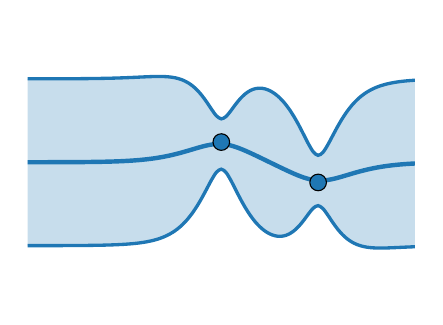
\begin{tikzpicture}
\begin{axis}[axis lines={none}, height={5cm}, width={6.5cm}, xmin={0}, xmax={1}, ymin={-1}, ymax={1}]
    \node at (0,-1) {};
    \node at (0,1) {};
    \node at (1,1) {};
    \node at (1,-1) {};
    \addplot[no markers, smooth, very thick, color={rgb,1:red,0.1216;green,0.4667;blue,0.7059}, name path={upper}]
        coordinates {
            (0.0,0.6199140961768654)
            (0.0125,0.6199425714927783)
            (0.025,0.6199783864581562)
            (0.0375,0.6200233662829112)
            (0.05,0.6200797656864601)
            (0.0625,0.6201503604553648)
            (0.075,0.6202385544841658)
            (0.0875,0.6203485030002299)
            (0.1,0.6204852515595847)
            (0.1125,0.6206548885126146)
            (0.125,0.6208647056109129)
            (0.1375,0.6211233567575545)
            (0.15,0.621440997918379)
            (0.1625,0.6218293810302168)
            (0.175,0.6223018602499781)
            (0.1875,0.6228732487414248)
            (0.2,0.6235594368715044)
            (0.2125,0.6243766466304895)
            (0.225,0.6253401510080454)
            (0.2375,0.6264622304388126)
            (0.25,0.6277490723629017)
            (0.2625,0.6291962483072014)
            (0.275,0.6307823339517931)
            (0.2875,0.6324601860223531)
            (0.3,0.6341453786837854)
            (0.3125,0.6357013651988239)
            (0.325,0.6369211143275115)
            (0.3375,0.6375053361068238)
            (0.35,0.6370380365657365)
            (0.3625,0.6349611286332626)
            (0.375,0.6305513230801723)
            (0.3875,0.6229047622218531)
            (0.4,0.6109382671624386)
            (0.4125,0.5934215336494578)
            (0.425,0.5690642064784973)
            (0.4375,0.5367009045678985)
            (0.45,0.49566153296827475)
            (0.4625,0.44653101260606376)
            (0.475,0.39282295507856513)
            (0.4875,0.34464685317516486)
            (0.5,0.3223754899538911)
            (0.5125,0.34058482839215576)
            (0.525,0.384306899691641)
            (0.5375,0.4328921481090502)
            (0.55,0.4759710490179375)
            (0.5625,0.5097228104055809)
            (0.575,0.5331850814547217)
            (0.5875,0.5465650120806383)
            (0.6,0.550466283604794)
            (0.6125,0.5455091311136459)
            (0.625,0.5321433216808108)
            (0.6375,0.5105731241442092)
            (0.65,0.48076057857831844)
            (0.6625,0.44249708250720937)
            (0.675,0.39555086340542395)
            (0.6875,0.3399197388696741)
            (0.7,0.27626172251086917)
            (0.7125,0.2066879756831459)
            (0.725,0.1364141076992448)
            (0.7375,0.07731047248583253)
            (0.75,0.05131933524894594)
            (0.7625,0.07391456195380275)
            (0.775,0.1297864344643398)
            (0.7875,0.19704165770173115)
            (0.8,0.2638428314974382)
            (0.8125,0.3250571025562066)
            (0.825,0.37873286688001917)
            (0.8375,0.4244703945004936)
            (0.85,0.4626524185492334)
            (0.8625,0.4940380860362959)
            (0.875,0.5195326231804909)
            (0.8875,0.5400545925834024)
            (0.9,0.5564623693375389)
            (0.9125,0.5695178886612947)
            (0.925,0.5798737501423057)
            (0.9375,0.5880743919367857)
            (0.95,0.5945650652582235)
            (0.9625,0.5997044498028763)
            (0.975,0.6037782650292838)
            (0.9875,0.6070123114982292)
            (1.0,0.609584123231418)
        }
        ;
    \addplot[no markers, smooth, very thick, color={rgb,1:red,0.1216;green,0.4667;blue,0.7059}, name path={lower}]
        coordinates {
            (0.0,-0.6196984280758382)
            (0.0125,-0.6196697615027457)
            (0.025,-0.6196336420765757)
            (0.0375,-0.6195881786813756)
            (0.05,-0.6195310130566563)
            (0.0625,-0.6194592072375776)
            (0.075,-0.6193691041152474)
            (0.0875,-0.6192561544448133)
            (0.1,-0.619114701753299)
            (0.1125,-0.6189377140916881)
            (0.125,-0.6187164481996643)
            (0.1375,-0.6184400270871517)
            (0.15,-0.6180949058637912)
            (0.1625,-0.6176641923303977)
            (0.175,-0.6171267777354612)
            (0.1875,-0.6164562184610327)
            (0.2,-0.6156192905043797)
            (0.2125,-0.6145741149161671)
            (0.225,-0.6132677238051523)
            (0.2375,-0.6116329041373474)
            (0.25,-0.609584123231418)
            (0.2625,-0.6070123114982292)
            (0.275,-0.6037782650292838)
            (0.2875,-0.5997044498028763)
            (0.3,-0.5945650652582235)
            (0.3125,-0.5880743919367857)
            (0.325,-0.5798737501423057)
            (0.3375,-0.5695178886612947)
            (0.35,-0.5564623693375389)
            (0.3625,-0.5400545925834024)
            (0.375,-0.5195326231804909)
            (0.3875,-0.4940380860362959)
            (0.4,-0.4626524185492334)
            (0.4125,-0.4244703945004936)
            (0.425,-0.37873286688001917)
            (0.4375,-0.3250571025562066)
            (0.45,-0.26384283149743815)
            (0.4625,-0.1970416577017311)
            (0.475,-0.12978643446433968)
            (0.4875,-0.07391456195380261)
            (0.5,-0.05131933524894591)
            (0.5125,-0.07731047248583231)
            (0.525,-0.13641410769924478)
            (0.5375,-0.2066879756831459)
            (0.55,-0.2762617225108691)
            (0.5625,-0.33991973886967414)
            (0.575,-0.3955508634054239)
            (0.5875,-0.4424970825072093)
            (0.6,-0.4807605785783184)
            (0.6125,-0.5105731241442092)
            (0.625,-0.5321433216808108)
            (0.6375,-0.5455091311136459)
            (0.65,-0.550466283604794)
            (0.6625,-0.5465650120806383)
            (0.675,-0.5331850814547217)
            (0.6875,-0.5097228104055808)
            (0.7,-0.4759710490179376)
            (0.7125,-0.4328921481090502)
            (0.725,-0.384306899691641)
            (0.7375,-0.340584828392156)
            (0.75,-0.32237548995389104)
            (0.7625,-0.34464685317516497)
            (0.775,-0.39282295507856524)
            (0.7875,-0.4465310126060638)
            (0.8,-0.4956615329682747)
            (0.8125,-0.5367009045678985)
            (0.825,-0.5690642064784973)
            (0.8375,-0.5934215336494578)
            (0.85,-0.6109382671624386)
            (0.8625,-0.6229047622218531)
            (0.875,-0.6305513230801723)
            (0.8875,-0.6349611286332626)
            (0.9,-0.6370380365657365)
            (0.9125,-0.6375053361068238)
            (0.925,-0.6369211143275115)
            (0.9375,-0.6357013651988239)
            (0.95,-0.6341453786837854)
            (0.9625,-0.6324601860223531)
            (0.975,-0.6307823339517931)
            (0.9875,-0.6291962483072014)
            (1.0,-0.6277490723629017)
        }
        ;
    \addplot[color={rgb,1:red,0.1216;green,0.4667;blue,0.7059}, opacity={0.25}]
        fill between [of = upper and lower]
        ;
    \addplot[no markers, smooth, ultra thick, color={rgb,1:red,0.1216;green,0.4667;blue,0.7059}]
        coordinates {
            (0.0,0.0001078340505135923)
            (0.0125,0.00013640499501634866)
            (0.025,0.00017237219079020152)
            (0.0375,0.0002175938007678534)
            (0.05,0.0002743763149019563)
            (0.0625,0.0003455766088936026)
            (0.075,0.00043472518445922124)
            (0.0875,0.0005461742777083397)
            (0.1,0.000685274903142837)
            (0.1125,0.000858587210463329)
            (0.125,0.001074128705624313)
            (0.1375,0.001341664835201373)
            (0.15,0.0016730460272938975)
            (0.1625,0.0020825943499095264)
            (0.175,0.0025875412572585045)
            (0.1875,0.0032085151401960847)
            (0.2,0.003970073183562359)
            (0.2125,0.00490126585716125)
            (0.225,0.006036213601446627)
            (0.2375,0.007414663150732556)
            (0.25,0.009082474565741901)
            (0.2625,0.011091968404486107)
            (0.275,0.013502034461254683)
            (0.2875,0.016377868109738417)
            (0.3,0.019790156712780962)
            (0.3125,0.023813486631019086)
            (0.325,0.02852368209260293)
            (0.3375,0.03399372372276454)
            (0.35,0.04028783361409879)
            (0.3625,0.04745326802493011)
            (0.375,0.055509349949840706)
            (0.3875,0.06443333809277857)
            (0.4,0.07414292430660259)
            (0.4125,0.0844755695744821)
            (0.425,0.0951656697992391)
            (0.4375,0.10582190100584594)
            (0.45,0.11590935073541828)
            (0.4625,0.12474467745216633)
            (0.475,0.13151826030711272)
            (0.4875,0.1353661456106811)
            (0.5,0.13552807735247258)
            (0.5125,0.13163717795316174)
            (0.525,0.1239463959961981)
            (0.5375,0.11310208621295215)
            (0.55,0.09985466325353423)
            (0.5625,0.08490153576795335)
            (0.575,0.06881710902464885)
            (0.5875,0.052033964786714494)
            (0.6,0.034852852513237824)
            (0.6125,0.017468003484718372)
            (0.625,1.3877787807814457e-17)
            (0.6375,-0.017468003484718365)
            (0.65,-0.0348528525132378)
            (0.6625,-0.05203396478671447)
            (0.675,-0.06881710902464883)
            (0.6875,-0.08490153576795334)
            (0.7,-0.09985466325353419)
            (0.7125,-0.11310208621295215)
            (0.725,-0.12394639599619808)
            (0.7375,-0.13163717795316174)
            (0.75,-0.13552807735247255)
            (0.7625,-0.1353661456106811)
            (0.775,-0.13151826030711272)
            (0.7875,-0.12474467745216633)
            (0.8,-0.11590935073541825)
            (0.8125,-0.10582190100584593)
            (0.825,-0.09516566979923907)
            (0.8375,-0.08447556957448209)
            (0.85,-0.07414292430660258)
            (0.8625,-0.06443333809277857)
            (0.875,-0.05550934994984069)
            (0.8875,-0.047453268024930106)
            (0.9,-0.04028783361409878)
            (0.9125,-0.03399372372276453)
            (0.925,-0.028523682092602927)
            (0.9375,-0.023813486631019083)
            (0.95,-0.01979015671278096)
            (0.9625,-0.016377868109738413)
            (0.975,-0.013502034461254682)
            (0.9875,-0.011091968404486105)
            (1.0,-0.0090824745657419)
        }
        ;
    \addplot[only marks, mark size={3pt}, fill={rgb,1:red,0.1216;green,0.4667;blue,0.7059}]
        coordinates {
            (0.5,0.15)
            (0.75,-0.15)
        }
        ;
\end{axis}
\end{tikzpicture}
\end{document}

\caption{Calculate conditional}
\end{subfigure}
\begin{subfigure}{0.49\textwidth}
\documentclass[tikz]{standalone}
\usepackage{pgfplots}
\pgfplotsset{compat=1.17}
\usepgfplotslibrary{external}
\usepgfplotslibrary{groupplots}
\usepgfplotslibrary{fillbetween}
\usetikzlibrary{fadings}
\begin{document}
\tikzsetnextfilename{figures/tex/gp-dist-samples.pdf}
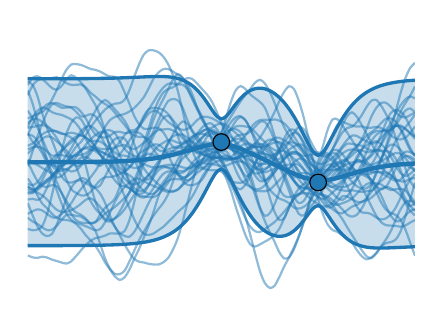
\begin{tikzpicture}
\begin{axis}[axis lines={none}, height={5cm}, width={6.5cm}, xmin={0}, xmax={1}, ymin={-1}, ymax={1}]
    \node at (0,-1) {};
    \node at (0,1) {};
    \node at (1,1) {};
    \node at (1,-1) {};
    \addplot[no markers, smooth, very thick, color={rgb,1:red,0.1216;green,0.4667;blue,0.7059}, name path={upper}]
        coordinates {
            (0.0,0.6199140961768654)
            (0.0125,0.6199425714927783)
            (0.025,0.6199783864581562)
            (0.0375,0.6200233662829112)
            (0.05,0.6200797656864601)
            (0.0625,0.6201503604553648)
            (0.075,0.6202385544841658)
            (0.0875,0.6203485030002299)
            (0.1,0.6204852515595847)
            (0.1125,0.6206548885126146)
            (0.125,0.6208647056109129)
            (0.1375,0.6211233567575545)
            (0.15,0.621440997918379)
            (0.1625,0.6218293810302168)
            (0.175,0.6223018602499781)
            (0.1875,0.6228732487414248)
            (0.2,0.6235594368715044)
            (0.2125,0.6243766466304895)
            (0.225,0.6253401510080454)
            (0.2375,0.6264622304388126)
            (0.25,0.6277490723629017)
            (0.2625,0.6291962483072014)
            (0.275,0.6307823339517931)
            (0.2875,0.6324601860223531)
            (0.3,0.6341453786837854)
            (0.3125,0.6357013651988239)
            (0.325,0.6369211143275115)
            (0.3375,0.6375053361068238)
            (0.35,0.6370380365657365)
            (0.3625,0.6349611286332626)
            (0.375,0.6305513230801723)
            (0.3875,0.6229047622218531)
            (0.4,0.6109382671624386)
            (0.4125,0.5934215336494578)
            (0.425,0.5690642064784973)
            (0.4375,0.5367009045678985)
            (0.45,0.49566153296827475)
            (0.4625,0.44653101260606376)
            (0.475,0.39282295507856513)
            (0.4875,0.34464685317516486)
            (0.5,0.3223754899538911)
            (0.5125,0.34058482839215576)
            (0.525,0.384306899691641)
            (0.5375,0.4328921481090502)
            (0.55,0.4759710490179375)
            (0.5625,0.5097228104055809)
            (0.575,0.5331850814547217)
            (0.5875,0.5465650120806383)
            (0.6,0.550466283604794)
            (0.6125,0.5455091311136459)
            (0.625,0.5321433216808108)
            (0.6375,0.5105731241442092)
            (0.65,0.48076057857831844)
            (0.6625,0.44249708250720937)
            (0.675,0.39555086340542395)
            (0.6875,0.3399197388696741)
            (0.7,0.27626172251086917)
            (0.7125,0.2066879756831459)
            (0.725,0.1364141076992448)
            (0.7375,0.07731047248583253)
            (0.75,0.05131933524894594)
            (0.7625,0.07391456195380275)
            (0.775,0.1297864344643398)
            (0.7875,0.19704165770173115)
            (0.8,0.2638428314974382)
            (0.8125,0.3250571025562066)
            (0.825,0.37873286688001917)
            (0.8375,0.4244703945004936)
            (0.85,0.4626524185492334)
            (0.8625,0.4940380860362959)
            (0.875,0.5195326231804909)
            (0.8875,0.5400545925834024)
            (0.9,0.5564623693375389)
            (0.9125,0.5695178886612947)
            (0.925,0.5798737501423057)
            (0.9375,0.5880743919367857)
            (0.95,0.5945650652582235)
            (0.9625,0.5997044498028763)
            (0.975,0.6037782650292838)
            (0.9875,0.6070123114982292)
            (1.0,0.609584123231418)
        }
        ;
    \addplot[no markers, smooth, very thick, color={rgb,1:red,0.1216;green,0.4667;blue,0.7059}, name path={lower}]
        coordinates {
            (0.0,-0.6196984280758382)
            (0.0125,-0.6196697615027457)
            (0.025,-0.6196336420765757)
            (0.0375,-0.6195881786813756)
            (0.05,-0.6195310130566563)
            (0.0625,-0.6194592072375776)
            (0.075,-0.6193691041152474)
            (0.0875,-0.6192561544448133)
            (0.1,-0.619114701753299)
            (0.1125,-0.6189377140916881)
            (0.125,-0.6187164481996643)
            (0.1375,-0.6184400270871517)
            (0.15,-0.6180949058637912)
            (0.1625,-0.6176641923303977)
            (0.175,-0.6171267777354612)
            (0.1875,-0.6164562184610327)
            (0.2,-0.6156192905043797)
            (0.2125,-0.6145741149161671)
            (0.225,-0.6132677238051523)
            (0.2375,-0.6116329041373474)
            (0.25,-0.609584123231418)
            (0.2625,-0.6070123114982292)
            (0.275,-0.6037782650292838)
            (0.2875,-0.5997044498028763)
            (0.3,-0.5945650652582235)
            (0.3125,-0.5880743919367857)
            (0.325,-0.5798737501423057)
            (0.3375,-0.5695178886612947)
            (0.35,-0.5564623693375389)
            (0.3625,-0.5400545925834024)
            (0.375,-0.5195326231804909)
            (0.3875,-0.4940380860362959)
            (0.4,-0.4626524185492334)
            (0.4125,-0.4244703945004936)
            (0.425,-0.37873286688001917)
            (0.4375,-0.3250571025562066)
            (0.45,-0.26384283149743815)
            (0.4625,-0.1970416577017311)
            (0.475,-0.12978643446433968)
            (0.4875,-0.07391456195380261)
            (0.5,-0.05131933524894591)
            (0.5125,-0.07731047248583231)
            (0.525,-0.13641410769924478)
            (0.5375,-0.2066879756831459)
            (0.55,-0.2762617225108691)
            (0.5625,-0.33991973886967414)
            (0.575,-0.3955508634054239)
            (0.5875,-0.4424970825072093)
            (0.6,-0.4807605785783184)
            (0.6125,-0.5105731241442092)
            (0.625,-0.5321433216808108)
            (0.6375,-0.5455091311136459)
            (0.65,-0.550466283604794)
            (0.6625,-0.5465650120806383)
            (0.675,-0.5331850814547217)
            (0.6875,-0.5097228104055808)
            (0.7,-0.4759710490179376)
            (0.7125,-0.4328921481090502)
            (0.725,-0.384306899691641)
            (0.7375,-0.340584828392156)
            (0.75,-0.32237548995389104)
            (0.7625,-0.34464685317516497)
            (0.775,-0.39282295507856524)
            (0.7875,-0.4465310126060638)
            (0.8,-0.4956615329682747)
            (0.8125,-0.5367009045678985)
            (0.825,-0.5690642064784973)
            (0.8375,-0.5934215336494578)
            (0.85,-0.6109382671624386)
            (0.8625,-0.6229047622218531)
            (0.875,-0.6305513230801723)
            (0.8875,-0.6349611286332626)
            (0.9,-0.6370380365657365)
            (0.9125,-0.6375053361068238)
            (0.925,-0.6369211143275115)
            (0.9375,-0.6357013651988239)
            (0.95,-0.6341453786837854)
            (0.9625,-0.6324601860223531)
            (0.975,-0.6307823339517931)
            (0.9875,-0.6291962483072014)
            (1.0,-0.6277490723629017)
        }
        ;
    \addplot[color={rgb,1:red,0.1216;green,0.4667;blue,0.7059}, opacity={0.25}]
        fill between [of = upper and lower]
        ;
    \addplot[no markers, smooth, ultra thick, color={rgb,1:red,0.1216;green,0.4667;blue,0.7059}]
        coordinates {
            (0.0,0.0001078340505135923)
            (0.0125,0.00013640499501634866)
            (0.025,0.00017237219079020152)
            (0.0375,0.0002175938007678534)
            (0.05,0.0002743763149019563)
            (0.0625,0.0003455766088936026)
            (0.075,0.00043472518445922124)
            (0.0875,0.0005461742777083397)
            (0.1,0.000685274903142837)
            (0.1125,0.000858587210463329)
            (0.125,0.001074128705624313)
            (0.1375,0.001341664835201373)
            (0.15,0.0016730460272938975)
            (0.1625,0.0020825943499095264)
            (0.175,0.0025875412572585045)
            (0.1875,0.0032085151401960847)
            (0.2,0.003970073183562359)
            (0.2125,0.00490126585716125)
            (0.225,0.006036213601446627)
            (0.2375,0.007414663150732556)
            (0.25,0.009082474565741901)
            (0.2625,0.011091968404486107)
            (0.275,0.013502034461254683)
            (0.2875,0.016377868109738417)
            (0.3,0.019790156712780962)
            (0.3125,0.023813486631019086)
            (0.325,0.02852368209260293)
            (0.3375,0.03399372372276454)
            (0.35,0.04028783361409879)
            (0.3625,0.04745326802493011)
            (0.375,0.055509349949840706)
            (0.3875,0.06443333809277857)
            (0.4,0.07414292430660259)
            (0.4125,0.0844755695744821)
            (0.425,0.0951656697992391)
            (0.4375,0.10582190100584594)
            (0.45,0.11590935073541828)
            (0.4625,0.12474467745216633)
            (0.475,0.13151826030711272)
            (0.4875,0.1353661456106811)
            (0.5,0.13552807735247258)
            (0.5125,0.13163717795316174)
            (0.525,0.1239463959961981)
            (0.5375,0.11310208621295215)
            (0.55,0.09985466325353423)
            (0.5625,0.08490153576795335)
            (0.575,0.06881710902464885)
            (0.5875,0.052033964786714494)
            (0.6,0.034852852513237824)
            (0.6125,0.017468003484718372)
            (0.625,1.3877787807814457e-17)
            (0.6375,-0.017468003484718365)
            (0.65,-0.0348528525132378)
            (0.6625,-0.05203396478671447)
            (0.675,-0.06881710902464883)
            (0.6875,-0.08490153576795334)
            (0.7,-0.09985466325353419)
            (0.7125,-0.11310208621295215)
            (0.725,-0.12394639599619808)
            (0.7375,-0.13163717795316174)
            (0.75,-0.13552807735247255)
            (0.7625,-0.1353661456106811)
            (0.775,-0.13151826030711272)
            (0.7875,-0.12474467745216633)
            (0.8,-0.11590935073541825)
            (0.8125,-0.10582190100584593)
            (0.825,-0.09516566979923907)
            (0.8375,-0.08447556957448209)
            (0.85,-0.07414292430660258)
            (0.8625,-0.06443333809277857)
            (0.875,-0.05550934994984069)
            (0.8875,-0.047453268024930106)
            (0.9,-0.04028783361409878)
            (0.9125,-0.03399372372276453)
            (0.925,-0.028523682092602927)
            (0.9375,-0.023813486631019083)
            (0.95,-0.01979015671278096)
            (0.9625,-0.016377868109738413)
            (0.975,-0.013502034461254682)
            (0.9875,-0.011091968404486105)
            (1.0,-0.0090824745657419)
        }
        ;
    \addplot[no markers, smooth, thick, color={rgb,1:red,0.1216;green,0.4667;blue,0.7059}, opacity={0.5}]
        coordinates {
            (0.0,0.09411852510663664)
            (0.0125,0.11223045819979174)
            (0.025,0.11502944275269632)
            (0.0375,0.10622193528465952)
            (0.05,0.08063759773341582)
            (0.0625,0.04939000441231901)
            (0.075,0.05232188632663536)
            (0.0875,0.05296575339322151)
            (0.1,0.0451423421644005)
            (0.1125,0.04282835178196053)
            (0.125,0.05339988746141579)
            (0.1375,0.08402876315544859)
            (0.15,0.13004542856915252)
            (0.1625,0.17018766633445273)
            (0.175,0.2017742333586193)
            (0.1875,0.22397609884577635)
            (0.2,0.2262283500586556)
            (0.2125,0.18826099298715718)
            (0.225,0.1264468186434583)
            (0.2375,0.05232713935217239)
            (0.25,-0.044218802413735464)
            (0.2625,-0.13503768301479604)
            (0.275,-0.193336661615306)
            (0.2875,-0.21325423874168098)
            (0.3,-0.20664367068562495)
            (0.3125,-0.16775411047703923)
            (0.325,-0.1098177976417911)
            (0.3375,-0.059614765970084534)
            (0.35,-0.03844356454254829)
            (0.3625,-0.03794974721976819)
            (0.375,-0.04497933080631564)
            (0.3875,-0.07722063789196243)
            (0.4,-0.11989777408047174)
            (0.4125,-0.13467000635647763)
            (0.425,-0.11194438256407474)
            (0.4375,-0.05829092513204907)
            (0.45,0.010366331865078904)
            (0.4625,0.06734498737050579)
            (0.475,0.09807114445833993)
            (0.4875,0.08674789950473306)
            (0.5,0.03199337347907287)
            (0.5125,-0.04634962817455843)
            (0.525,-0.12442895934165456)
            (0.5375,-0.18453018943262517)
            (0.55,-0.20053671687393262)
            (0.5625,-0.16505028600726596)
            (0.575,-0.10082108805900963)
            (0.5875,-0.04652443240997973)
            (0.6,-0.023722504274527045)
            (0.6125,-0.010201357621905292)
            (0.625,-0.01605515376932381)
            (0.6375,-0.023224495788528903)
            (0.65,-0.026433264207334238)
            (0.6625,-0.022043187252101033)
            (0.675,-0.01696706516188929)
            (0.6875,-0.02329028991451399)
            (0.7,-0.0632445085890709)
            (0.7125,-0.12412917321967713)
            (0.725,-0.1914371048215351)
            (0.7375,-0.22205594810437296)
            (0.75,-0.23344439614311013)
            (0.7625,-0.2467665963677519)
            (0.775,-0.2720437777505848)
            (0.7875,-0.319634015249627)
            (0.8,-0.37232393196909574)
            (0.8125,-0.4217277733119887)
            (0.825,-0.48322318499953615)
            (0.8375,-0.5404757474982456)
            (0.85,-0.5973686848576143)
            (0.8625,-0.6526514019902161)
            (0.875,-0.6985448429515345)
            (0.8875,-0.7126504977913749)
            (0.9,-0.6785286001996675)
            (0.9125,-0.6289869249454848)
            (0.925,-0.6006053281431735)
            (0.9375,-0.5932153394314362)
            (0.95,-0.5740795233620173)
            (0.9625,-0.5167154329033531)
            (0.975,-0.40512286537609965)
            (0.9875,-0.2790838127772967)
            (1.0,-0.15136538919261402)
        }
        ;
    \addplot[no markers, smooth, thick, color={rgb,1:red,0.1216;green,0.4667;blue,0.7059}, opacity={0.5}]
        coordinates {
            (0.0,-0.15960997729156717)
            (0.0125,-0.17100679657571016)
            (0.025,-0.14913369071153396)
            (0.0375,-0.09572714958472996)
            (0.05,-0.032475455626117075)
            (0.0625,0.018863440829643054)
            (0.075,0.05705816686924676)
            (0.0875,0.08916558996181921)
            (0.1,0.11922630291840797)
            (0.1125,0.14783629647734167)
            (0.125,0.17737023929432433)
            (0.1375,0.20619812312764366)
            (0.15,0.24945583108426986)
            (0.1625,0.31563038786719116)
            (0.175,0.3835137926582052)
            (0.1875,0.4379685415126771)
            (0.2,0.4623360473339842)
            (0.2125,0.4355062783235683)
            (0.225,0.3937327455505968)
            (0.2375,0.3537659345178087)
            (0.25,0.3093976914962435)
            (0.2625,0.24221988580693554)
            (0.275,0.13628004916209374)
            (0.2875,0.03497145630038323)
            (0.3,-0.04518178387050452)
            (0.3125,-0.09260242421713752)
            (0.325,-0.1307452834631939)
            (0.3375,-0.16448855485640893)
            (0.35,-0.1946852621213295)
            (0.3625,-0.21087551971800478)
            (0.375,-0.213601186192933)
            (0.3875,-0.20256485940368718)
            (0.4,-0.16234529890653582)
            (0.4125,-0.09512194813006883)
            (0.425,-0.035776745061475185)
            (0.4375,-0.002014935730278347)
            (0.45,0.021198911500351927)
            (0.4625,0.02782054786072155)
            (0.475,0.034466334334549625)
            (0.4875,0.03407968591367841)
            (0.5,0.008985782363270606)
            (0.5125,-0.04944046349382927)
            (0.525,-0.11489371282398929)
            (0.5375,-0.20468587835391816)
            (0.55,-0.30338317384890223)
            (0.5625,-0.40881247850750135)
            (0.575,-0.542143346089398)
            (0.5875,-0.6813316491521201)
            (0.6,-0.8119710111650108)
            (0.6125,-0.8975773104234512)
            (0.625,-0.9336293361760287)
            (0.6375,-0.9178285399822874)
            (0.65,-0.8509872577529835)
            (0.6625,-0.7732457437779044)
            (0.675,-0.7064542281875639)
            (0.6875,-0.6321709412063347)
            (0.7,-0.549875091302569)
            (0.7125,-0.44919710101235566)
            (0.725,-0.3169253231373974)
            (0.7375,-0.18027080732540868)
            (0.75,-0.06588902531017518)
            (0.7625,0.0010115465183940242)
            (0.775,0.05225016213105063)
            (0.7875,0.08712896983176072)
            (0.8,0.09011083111058199)
            (0.8125,0.06084213866150276)
            (0.825,0.01068786934453747)
            (0.8375,-0.037460870733703376)
            (0.85,-0.06550419527045408)
            (0.8625,-0.08092207430659294)
            (0.875,-0.09085325382233751)
            (0.8875,-0.0827392199837356)
            (0.9,-0.06999720435805704)
            (0.9125,-0.0796519547421)
            (0.925,-0.09979320518446272)
            (0.9375,-0.11885275654321885)
            (0.95,-0.13959494845309717)
            (0.9625,-0.12946761140365154)
            (0.975,-0.084103917507409)
            (0.9875,-0.037167714821120135)
            (1.0,-0.003758130646337624)
        }
        ;
    \addplot[no markers, smooth, thick, color={rgb,1:red,0.1216;green,0.4667;blue,0.7059}, opacity={0.5}]
        coordinates {
            (0.0,0.0193084897914274)
            (0.0125,0.005430003686234309)
            (0.025,-0.0054772938465677545)
            (0.0375,-0.003801692662627678)
            (0.05,-0.0077670257400072485)
            (0.0625,-0.018997559241232958)
            (0.075,-0.03205835625611805)
            (0.0875,-0.027073023516715655)
            (0.1,-0.004668800591463971)
            (0.1125,0.028081174648525418)
            (0.125,0.04990564573247902)
            (0.1375,0.054198270401691756)
            (0.15,0.06618719597217818)
            (0.1625,0.09726572911755972)
            (0.175,0.1420921054677759)
            (0.1875,0.19563047585551407)
            (0.2,0.2634323306598613)
            (0.2125,0.3131465596306925)
            (0.225,0.3364361016816288)
            (0.2375,0.34914533475109394)
            (0.25,0.3589560983289753)
            (0.2625,0.37671375711518423)
            (0.275,0.40340607024524705)
            (0.2875,0.43976250651376947)
            (0.3,0.48392357807296293)
            (0.3125,0.5495928487549122)
            (0.325,0.6213441607693896)
            (0.3375,0.666408659258694)
            (0.35,0.6914763332031165)
            (0.3625,0.6927671151496207)
            (0.375,0.6745811775513143)
            (0.3875,0.650408738586131)
            (0.4,0.6269118263580961)
            (0.4125,0.5789530336476498)
            (0.425,0.5048501624928714)
            (0.4375,0.40743344961558914)
            (0.45,0.3154515161114989)
            (0.4625,0.2649198934297313)
            (0.475,0.2238023056254852)
            (0.4875,0.18305165420764857)
            (0.5,0.15114353209268278)
            (0.5125,0.12567827970156925)
            (0.525,0.09523603009501212)
            (0.5375,0.0693820762908916)
            (0.55,0.02413797013062413)
            (0.5625,-0.046087523805716)
            (0.575,-0.13440764398227575)
            (0.5875,-0.2457977532758812)
            (0.6,-0.3460183843167228)
            (0.6125,-0.43738277805664594)
            (0.625,-0.519556494158)
            (0.6375,-0.5914745111683819)
            (0.65,-0.6695908447693328)
            (0.6625,-0.7146586275608865)
            (0.675,-0.7061519507347838)
            (0.6875,-0.6466776403590896)
            (0.7,-0.552871739739878)
            (0.7125,-0.44221393970578193)
            (0.725,-0.328083946749633)
            (0.7375,-0.23930080823476108)
            (0.75,-0.16677196970786834)
            (0.7625,-0.09885834653215277)
            (0.775,-0.051240025257067)
            (0.7875,-0.016879896613483547)
            (0.8,-0.0015547355633084292)
            (0.8125,-0.008675220359769462)
            (0.825,-0.03472117395923448)
            (0.8375,-0.05935321325059022)
            (0.85,-0.06264345230348449)
            (0.8625,-0.0677247805264157)
            (0.875,-0.06848413704810798)
            (0.8875,-0.07257207498326532)
            (0.9,-0.07147421576653719)
            (0.9125,-0.0740418994997428)
            (0.925,-0.07815629578253197)
            (0.9375,-0.09179003488231398)
            (0.95,-0.13217981266675438)
            (0.9625,-0.1948584934353904)
            (0.975,-0.26949008011714026)
            (0.9875,-0.3238089939405014)
            (1.0,-0.36158413680460366)
        }
        ;
    \addplot[no markers, smooth, thick, color={rgb,1:red,0.1216;green,0.4667;blue,0.7059}, opacity={0.5}]
        coordinates {
            (0.0,0.006865609797605608)
            (0.0125,-0.07159330896159946)
            (0.025,-0.13895919082512848)
            (0.0375,-0.1756364920979333)
            (0.05,-0.1831474582677916)
            (0.0625,-0.16949325331916462)
            (0.075,-0.17982173080335886)
            (0.0875,-0.22706413629624447)
            (0.1,-0.2884156987528625)
            (0.1125,-0.3395482272191261)
            (0.125,-0.3727798447908525)
            (0.1375,-0.390280254372352)
            (0.15,-0.4183533412563598)
            (0.1625,-0.4599183297292635)
            (0.175,-0.5106806291744216)
            (0.1875,-0.6083955793483625)
            (0.2,-0.7158430104323981)
            (0.2125,-0.7903708853037356)
            (0.225,-0.8290510387184247)
            (0.2375,-0.8312889031949927)
            (0.25,-0.8067299416478844)
            (0.2625,-0.7379424547101199)
            (0.275,-0.6585601441754926)
            (0.2875,-0.5787366590980028)
            (0.3,-0.5153626306742597)
            (0.3125,-0.45297202859607566)
            (0.325,-0.3961380603465553)
            (0.3375,-0.34737566277112963)
            (0.35,-0.3022783292839485)
            (0.3625,-0.23912628682146786)
            (0.375,-0.14625628692171766)
            (0.3875,-0.04066188045522827)
            (0.4,0.06131970956511663)
            (0.4125,0.13098290640803878)
            (0.425,0.17325641456268615)
            (0.4375,0.21349227386630515)
            (0.45,0.25732847383608204)
            (0.4625,0.2841864403614659)
            (0.475,0.2878921300933743)
            (0.4875,0.24810149071016416)
            (0.5,0.19730067448337404)
            (0.5125,0.14718404166897972)
            (0.525,0.10493291059585394)
            (0.5375,0.07372753586946557)
            (0.55,0.052420952867683744)
            (0.5625,0.03176056319873233)
            (0.575,0.013282328536826364)
            (0.5875,-0.0034153565937399336)
            (0.6,-0.013580584021851812)
            (0.6125,-0.00328287118586466)
            (0.625,0.020708567006683245)
            (0.6375,0.05641536712357854)
            (0.65,0.07517632696554)
            (0.6625,0.0993476351911773)
            (0.675,0.14960277521794776)
            (0.6875,0.2188126012925075)
            (0.7,0.2604100257859438)
            (0.7125,0.2474150681865544)
            (0.725,0.1891300127022196)
            (0.7375,0.11811023868794021)
            (0.75,0.06105484186684393)
            (0.7625,0.04409210785526746)
            (0.775,0.037884426456726045)
            (0.7875,0.009458804373189744)
            (0.8,-0.02637988491510601)
            (0.8125,-0.052979002848110246)
            (0.825,-0.052922507710776875)
            (0.8375,-0.024150602309180647)
            (0.85,0.012804834255335615)
            (0.8625,0.0011366089156123471)
            (0.875,-0.06737230412995074)
            (0.8875,-0.1505319494216475)
            (0.9,-0.22122129132609797)
            (0.9125,-0.29699308129372026)
            (0.925,-0.3516242948776708)
            (0.9375,-0.37663454160469495)
            (0.95,-0.39112675275366515)
            (0.9625,-0.42740116226493735)
            (0.975,-0.49791839959954937)
            (0.9875,-0.5954101313037918)
            (1.0,-0.6947404553016164)
        }
        ;
    \addplot[no markers, smooth, thick, color={rgb,1:red,0.1216;green,0.4667;blue,0.7059}, opacity={0.5}]
        coordinates {
            (0.0,0.2609917166342367)
            (0.0125,0.3344361811490312)
            (0.025,0.380851572979921)
            (0.0375,0.40666178087409965)
            (0.05,0.3967208040000672)
            (0.0625,0.37306031663395256)
            (0.075,0.3593203098287789)
            (0.0875,0.3522753473202288)
            (0.1,0.33640646290065734)
            (0.1125,0.31883964507031204)
            (0.125,0.28783619152565343)
            (0.1375,0.23750536857045368)
            (0.15,0.1714935753791337)
            (0.1625,0.1192729871281514)
            (0.175,0.09595566906813283)
            (0.1875,0.07868372974974172)
            (0.2,0.06472453743387328)
            (0.2125,0.048909208356686454)
            (0.225,0.03467953007744408)
            (0.2375,0.0030679523616634827)
            (0.25,-0.06478469427873586)
            (0.2625,-0.15700415943934926)
            (0.275,-0.2216158597069462)
            (0.2875,-0.24617878748301708)
            (0.3,-0.253729584258325)
            (0.3125,-0.2575439363026032)
            (0.325,-0.25878249579065477)
            (0.3375,-0.23947697011928393)
            (0.35,-0.19983918553794147)
            (0.3625,-0.1515400342631283)
            (0.375,-0.09154062372264511)
            (0.3875,-0.026246878111274546)
            (0.4,0.026602698577266805)
            (0.4125,0.05702202365726804)
            (0.425,0.09223165361545281)
            (0.4375,0.13446387511327013)
            (0.45,0.18013574673985397)
            (0.4625,0.2145384178395761)
            (0.475,0.2281039714070532)
            (0.4875,0.21728994869824422)
            (0.5,0.19020450215103107)
            (0.5125,0.1639265264608922)
            (0.525,0.13735270104862093)
            (0.5375,0.09826242438801389)
            (0.55,0.061543153640263644)
            (0.5625,0.04522354468888587)
            (0.575,0.04824176164231925)
            (0.5875,0.05181836416992552)
            (0.6,0.04203301197043602)
            (0.6125,0.039746143512037466)
            (0.625,0.035195010124862376)
            (0.6375,0.012458099886377992)
            (0.65,-0.033424326814909186)
            (0.6625,-0.1181158264784114)
            (0.675,-0.21342618804722585)
            (0.6875,-0.30881220892680794)
            (0.7,-0.38277099358104044)
            (0.7125,-0.3949317752966906)
            (0.725,-0.35004305769259947)
            (0.7375,-0.3068661035177332)
            (0.75,-0.2571895898495764)
            (0.7625,-0.20526953318416646)
            (0.775,-0.15220755532449237)
            (0.7875,-0.09985064605931679)
            (0.8,-0.0617882034148732)
            (0.8125,-0.013761379021436412)
            (0.825,0.039332812871499145)
            (0.8375,0.08495993256057423)
            (0.85,0.12109456085097725)
            (0.8625,0.16043169254747836)
            (0.875,0.1970154625553301)
            (0.8875,0.22394727809275328)
            (0.9,0.25093742199464214)
            (0.9125,0.2901998958765029)
            (0.925,0.32372049942237535)
            (0.9375,0.3257244567477681)
            (0.95,0.30376027714989806)
            (0.9625,0.2446307509207088)
            (0.975,0.16407859633667637)
            (0.9875,0.09160807678030262)
            (1.0,0.04731820648053358)
        }
        ;
    \addplot[no markers, smooth, thick, color={rgb,1:red,0.1216;green,0.4667;blue,0.7059}, opacity={0.5}]
        coordinates {
            (0.0,-0.23116643615761112)
            (0.0125,-0.2296415190705382)
            (0.025,-0.2067153450239769)
            (0.0375,-0.17319614404918857)
            (0.05,-0.13568590603615943)
            (0.0625,-0.09768398488480462)
            (0.075,-0.06013901282984985)
            (0.0875,-0.026975984605498906)
            (0.1,0.008213425025905729)
            (0.1125,0.06236877117503102)
            (0.125,0.11489800104451316)
            (0.1375,0.15131097302842939)
            (0.15,0.20239881198298387)
            (0.1625,0.26025413313222817)
            (0.175,0.3087173045745282)
            (0.1875,0.3518343804227841)
            (0.2,0.3922018822245264)
            (0.2125,0.4182676497014175)
            (0.225,0.43542241662163933)
            (0.2375,0.4394389073834724)
            (0.25,0.4635734638107397)
            (0.2625,0.5346017594505325)
            (0.275,0.6340284980584006)
            (0.2875,0.7277824656393278)
            (0.3,0.8004367485728591)
            (0.3125,0.831323017500696)
            (0.325,0.8310830815416321)
            (0.3375,0.8179411247702396)
            (0.35,0.7852128735948349)
            (0.3625,0.7300586227924282)
            (0.375,0.6475190893001052)
            (0.3875,0.5311437639522842)
            (0.4,0.3829751930148574)
            (0.4125,0.22196263931391197)
            (0.425,0.0883074700084566)
            (0.4375,0.006899665898542184)
            (0.45,-0.0373943423503062)
            (0.4625,-0.0305260892984536)
            (0.475,0.02131097615620864)
            (0.4875,0.0813720787945382)
            (0.5,0.1385476763665924)
            (0.5125,0.1917725372727255)
            (0.525,0.2483317932168569)
            (0.5375,0.30765418038992093)
            (0.55,0.33702840311353255)
            (0.5625,0.3127038105059618)
            (0.575,0.2443207032399761)
            (0.5875,0.1814074144770489)
            (0.6,0.11960309405225752)
            (0.6125,0.04973646120424437)
            (0.625,-0.026759796812830475)
            (0.6375,-0.11733830058728076)
            (0.65,-0.19942673042766873)
            (0.6625,-0.24994134350825759)
            (0.675,-0.2589217949741025)
            (0.6875,-0.24942112610755565)
            (0.7,-0.23478606493583964)
            (0.7125,-0.20547666245854196)
            (0.725,-0.16101562586045626)
            (0.7375,-0.10332400645795595)
            (0.75,-0.02601770040926779)
            (0.7625,0.05127378114470452)
            (0.775,0.119744952215943)
            (0.7875,0.20594077946254913)
            (0.8,0.27758746952116853)
            (0.8125,0.3001437275910279)
            (0.825,0.2863153598287987)
            (0.8375,0.2727842363567888)
            (0.85,0.2649529225253024)
            (0.8625,0.26688861861090724)
            (0.875,0.2564781754681623)
            (0.8875,0.2569143445598166)
            (0.9,0.26270823246629715)
            (0.9125,0.2548123536830967)
            (0.925,0.23468703161287746)
            (0.9375,0.23687353126165453)
            (0.95,0.27392379626672353)
            (0.9625,0.3296438776616227)
            (0.975,0.38268383180878723)
            (0.9875,0.3997772964413712)
            (1.0,0.3711338202584603)
        }
        ;
    \addplot[no markers, smooth, thick, color={rgb,1:red,0.1216;green,0.4667;blue,0.7059}, opacity={0.5}]
        coordinates {
            (0.0,0.573377473657675)
            (0.0125,0.6271994376209008)
            (0.025,0.6388514585059555)
            (0.0375,0.6196916115792405)
            (0.05,0.5854400331553036)
            (0.0625,0.5521283276428756)
            (0.075,0.5396035918996456)
            (0.0875,0.5668059958328023)
            (0.1,0.6168470645794852)
            (0.1125,0.6460005667550631)
            (0.125,0.6278590417997584)
            (0.1375,0.593739064240556)
            (0.15,0.5463786366162684)
            (0.1625,0.4848614888120193)
            (0.175,0.42419225898108764)
            (0.1875,0.34245181622161114)
            (0.2,0.23288943947234556)
            (0.2125,0.11078508193668671)
            (0.225,0.003016925889626013)
            (0.2375,-0.06986487354333762)
            (0.25,-0.12136371409356642)
            (0.2625,-0.15292016937074548)
            (0.275,-0.16387290874698396)
            (0.2875,-0.1547839977808837)
            (0.3,-0.12573865802080836)
            (0.3125,-0.09391007032672655)
            (0.325,-0.058826773122116094)
            (0.3375,-0.038293161497976645)
            (0.35,-0.02993107265741802)
            (0.3625,-0.04185333757422525)
            (0.375,-0.06113530573921892)
            (0.3875,-0.08018784641998813)
            (0.4,-0.07721752007893949)
            (0.4125,-0.049313330974251945)
            (0.425,-0.00482802297607976)
            (0.4375,0.0329133119380768)
            (0.45,0.05635547556720972)
            (0.4625,0.0531681534424574)
            (0.475,0.033792808554919576)
            (0.4875,0.035599233054994656)
            (0.5,0.044194253444279824)
            (0.5125,0.0474745462157372)
            (0.525,0.03480937895448487)
            (0.5375,0.02428737541990922)
            (0.55,0.04360345489700633)
            (0.5625,0.07948786805899045)
            (0.575,0.11706129662967624)
            (0.5875,0.13848931860200991)
            (0.6,0.13639497071725198)
            (0.6125,0.11381160006773161)
            (0.625,0.08087675621211204)
            (0.6375,0.03876610020630321)
            (0.65,-0.01073979541547071)
            (0.6625,-0.05526818899600413)
            (0.675,-0.09261459922138211)
            (0.6875,-0.1335133501170501)
            (0.7,-0.17420305216145693)
            (0.7125,-0.19109716501006316)
            (0.725,-0.20043804035109486)
            (0.7375,-0.2305972343876696)
            (0.75,-0.2590983509482484)
            (0.7625,-0.27489220587275787)
            (0.775,-0.2552624830488286)
            (0.7875,-0.22305186503663882)
            (0.8,-0.1920694040769171)
            (0.8125,-0.15163769441920197)
            (0.825,-0.09756381864079695)
            (0.8375,-0.03452433148543033)
            (0.85,0.04123546026782213)
            (0.8625,0.09622128858811313)
            (0.875,0.12628085834089373)
            (0.8875,0.14676975488000002)
            (0.9,0.15567395895438707)
            (0.9125,0.13627479441366624)
            (0.925,0.0962152554471693)
            (0.9375,0.04201946061032509)
            (0.95,-0.023525217369216866)
            (0.9625,-0.0793160997596652)
            (0.975,-0.10219393990877795)
            (0.9875,-0.08732126475040694)
            (1.0,-0.05257581324215496)
        }
        ;
    \addplot[no markers, smooth, thick, color={rgb,1:red,0.1216;green,0.4667;blue,0.7059}, opacity={0.5}]
        coordinates {
            (0.0,-0.18333089235841774)
            (0.0125,-0.2030842145115882)
            (0.025,-0.22587719061947)
            (0.0375,-0.2456570099938953)
            (0.05,-0.2765391563186894)
            (0.0625,-0.31881029241711445)
            (0.075,-0.35325890870334997)
            (0.0875,-0.3675044748882133)
            (0.1,-0.3679979412607171)
            (0.1125,-0.35675117982392807)
            (0.125,-0.3357230490661414)
            (0.1375,-0.3089994616497897)
            (0.15,-0.2789274171486657)
            (0.1625,-0.26801989024247647)
            (0.175,-0.29200769953063427)
            (0.1875,-0.33373515464090303)
            (0.2,-0.3759309759083109)
            (0.2125,-0.4258514668862958)
            (0.225,-0.47992034788247007)
            (0.2375,-0.540191673764799)
            (0.25,-0.6102353728035409)
            (0.2625,-0.6700696199413115)
            (0.275,-0.7186287988593748)
            (0.2875,-0.7385343627920299)
            (0.3,-0.7448960694220019)
            (0.3125,-0.7545227163726669)
            (0.325,-0.7597594465249279)
            (0.3375,-0.759501671671275)
            (0.35,-0.7437022035625827)
            (0.3625,-0.7117951672667008)
            (0.375,-0.6494342287438158)
            (0.3875,-0.5652037677138742)
            (0.4,-0.44304540924183594)
            (0.4125,-0.3015037965959375)
            (0.425,-0.1580920856227279)
            (0.4375,-0.01623742690188787)
            (0.45,0.10918958128616733)
            (0.4625,0.18697041770101155)
            (0.475,0.21132326845127558)
            (0.4875,0.21194321361931126)
            (0.5,0.20695498141818908)
            (0.5125,0.20511940333438816)
            (0.525,0.1867125863452077)
            (0.5375,0.15410523323779815)
            (0.55,0.11246400784454062)
            (0.5625,0.06787552696175086)
            (0.575,0.01912285377803915)
            (0.5875,-0.02715916610761048)
            (0.6,-0.06586706631951386)
            (0.6125,-0.07476261942371916)
            (0.625,-0.06236907469593797)
            (0.6375,-0.0456603825605878)
            (0.65,-0.02071928998199864)
            (0.6625,0.02120319763111228)
            (0.675,0.05773110714916552)
            (0.6875,0.07448365934848658)
            (0.7,0.0676094849884412)
            (0.7125,0.021796687797242448)
            (0.725,-0.034283633360959936)
            (0.7375,-0.06603230753520163)
            (0.75,-0.07496840656004637)
            (0.7625,-0.029592295773782057)
            (0.775,0.03906001512454285)
            (0.7875,0.09744815116612837)
            (0.8,0.16001769792711412)
            (0.8125,0.22089798319515003)
            (0.825,0.25436142614219337)
            (0.8375,0.26469872397131133)
            (0.85,0.29787597644710073)
            (0.8625,0.3491684861341885)
            (0.875,0.4106900810161212)
            (0.8875,0.4573593224165604)
            (0.9,0.46333020489837057)
            (0.9125,0.4207019255391838)
            (0.925,0.35882581953487475)
            (0.9375,0.2863944643352678)
            (0.95,0.1855654036353711)
            (0.9625,0.07407088631613688)
            (0.975,-0.04273778393048422)
            (0.9875,-0.13794273346250363)
            (1.0,-0.19169499724654862)
        }
        ;
    \addplot[no markers, smooth, thick, color={rgb,1:red,0.1216;green,0.4667;blue,0.7059}, opacity={0.5}]
        coordinates {
            (0.0,0.6014774692020028)
            (0.0125,0.5752021541601241)
            (0.025,0.4935509945192089)
            (0.0375,0.3637077897980357)
            (0.05,0.25333316144157353)
            (0.0625,0.1645158339149042)
            (0.075,0.07093991882825637)
            (0.0875,-0.025477714109828915)
            (0.1,-0.1275620293028157)
            (0.1125,-0.20077168473320778)
            (0.125,-0.2272540613629279)
            (0.1375,-0.2459156827695675)
            (0.15,-0.24488066475559958)
            (0.1625,-0.22081897096854408)
            (0.175,-0.17451098096475007)
            (0.1875,-0.13239764916457195)
            (0.2,-0.1116703549357088)
            (0.2125,-0.1094159878783758)
            (0.225,-0.10216944709308566)
            (0.2375,-0.08789760370945508)
            (0.25,-0.06649037422013192)
            (0.2625,-0.03294143230501062)
            (0.275,0.0024499892490165345)
            (0.2875,0.05912188940803782)
            (0.3,0.14466496522941624)
            (0.3125,0.2513482213971013)
            (0.325,0.3662003227238694)
            (0.3375,0.4579347631064829)
            (0.35,0.5170882242531534)
            (0.3625,0.5443311571066145)
            (0.375,0.5565823279934234)
            (0.3875,0.5814140062547721)
            (0.4,0.6081792290061717)
            (0.4125,0.624970742053478)
            (0.425,0.6188706121047242)
            (0.4375,0.5847998006855428)
            (0.45,0.5445678679646089)
            (0.4625,0.5048218607280788)
            (0.475,0.45448309427327044)
            (0.4875,0.37839183366614615)
            (0.5,0.29047554846664647)
            (0.5125,0.20661632970447186)
            (0.525,0.12415885497967993)
            (0.5375,0.03644136628733835)
            (0.55,-0.04856197942232804)
            (0.5625,-0.10202851138663242)
            (0.575,-0.0885963699356514)
            (0.5875,-0.010576251054226125)
            (0.6,0.08552898817991667)
            (0.6125,0.14725129066274611)
            (0.625,0.1685817921822409)
            (0.6375,0.16469929665437552)
            (0.65,0.14069458784338723)
            (0.6625,0.08931354472842894)
            (0.675,0.017974280321948727)
            (0.6875,-0.0642249992288538)
            (0.7,-0.1256896432944307)
            (0.7125,-0.16963690897274997)
            (0.725,-0.19716746082146552)
            (0.7375,-0.20088364773665615)
            (0.75,-0.1813299262540148)
            (0.7625,-0.1719816747751351)
            (0.775,-0.1974678743323544)
            (0.7875,-0.22937610000817626)
            (0.8,-0.2667591473229832)
            (0.8125,-0.27957848729264595)
            (0.825,-0.2531351006703446)
            (0.8375,-0.19859556053655206)
            (0.85,-0.12272506276729461)
            (0.8625,-0.044437467341995385)
            (0.875,0.013822999304479819)
            (0.8875,0.046815030541518296)
            (0.9,0.089656898983043)
            (0.9125,0.13234908708777743)
            (0.925,0.19093091901295373)
            (0.9375,0.24268573620721215)
            (0.95,0.27065990516501404)
            (0.9625,0.26596074821286725)
            (0.975,0.24650505415612758)
            (0.9875,0.2168485042455825)
            (1.0,0.18927827907147257)
        }
        ;
    \addplot[no markers, smooth, thick, color={rgb,1:red,0.1216;green,0.4667;blue,0.7059}, opacity={0.5}]
        coordinates {
            (0.0,-0.19961024748210288)
            (0.0125,-0.2126154759809669)
            (0.025,-0.18974465623684098)
            (0.0375,-0.15429082727327895)
            (0.05,-0.1286256035194636)
            (0.0625,-0.10498657780461626)
            (0.075,-0.06119911075904908)
            (0.0875,-2.404905831974969e-5)
            (0.1,0.04815176588062828)
            (0.1125,0.10328889503792067)
            (0.125,0.17027257549963531)
            (0.1375,0.23198468065465644)
            (0.15,0.2605087864987418)
            (0.1625,0.2685977610929211)
            (0.175,0.2433638425978437)
            (0.1875,0.19816129566115573)
            (0.2,0.1310552157457833)
            (0.2125,0.04839324212995069)
            (0.225,-0.05229846300243041)
            (0.2375,-0.1611782704501607)
            (0.25,-0.25116149231202534)
            (0.2625,-0.3374069735954111)
            (0.275,-0.42337594171077136)
            (0.2875,-0.48920398258370423)
            (0.3,-0.5319478169951921)
            (0.3125,-0.5398436777049664)
            (0.325,-0.5296216282613502)
            (0.3375,-0.504736045149233)
            (0.35,-0.4802923473933884)
            (0.3625,-0.44538795949696386)
            (0.375,-0.40967263032542406)
            (0.3875,-0.37041679138182493)
            (0.4,-0.3392235112847592)
            (0.4125,-0.30407462805809854)
            (0.425,-0.25427031703784786)
            (0.4375,-0.18800613168566)
            (0.45,-0.11121151359943185)
            (0.4625,-0.057413204284245845)
            (0.475,-0.019692053484038408)
            (0.4875,0.004993625069325491)
            (0.5,0.015222988470194335)
            (0.5125,0.01178407782741954)
            (0.525,0.019088839068513372)
            (0.5375,0.024745641152969053)
            (0.55,0.015945395625723502)
            (0.5625,-0.013630424521894433)
            (0.575,-0.054608459090451936)
            (0.5875,-0.08375987143764166)
            (0.6,-0.07872924195693323)
            (0.6125,-0.05876418038624888)
            (0.625,-0.020668506670895117)
            (0.6375,0.03261254478493577)
            (0.65,0.08452341594600957)
            (0.6625,0.1273087373277289)
            (0.675,0.14706255005950944)
            (0.6875,0.1455771313541943)
            (0.7,0.12599492102770343)
            (0.7125,0.0930241691814781)
            (0.725,0.04964476240420229)
            (0.7375,0.013766107364682006)
            (0.75,-0.009670777279637693)
            (0.7625,-0.010910169918498261)
            (0.775,0.00640548805297661)
            (0.7875,0.03411208601450455)
            (0.8,0.07218806070014402)
            (0.8125,0.11927685590120815)
            (0.825,0.16689710588120266)
            (0.8375,0.198052893453448)
            (0.85,0.19552385805225553)
            (0.8625,0.17388523913481305)
            (0.875,0.15522523099215785)
            (0.8875,0.13900245211231493)
            (0.9,0.14533369671102642)
            (0.9125,0.1771118986684031)
            (0.925,0.22123596154780753)
            (0.9375,0.24586281045472272)
            (0.95,0.26843841029118565)
            (0.9625,0.2732189769033388)
            (0.975,0.25100546041372496)
            (0.9875,0.215435937496343)
            (1.0,0.1731153957604772)
        }
        ;
    \addplot[no markers, smooth, thick, color={rgb,1:red,0.1216;green,0.4667;blue,0.7059}, opacity={0.5}]
        coordinates {
            (0.0,-0.3835618928824108)
            (0.0125,-0.36461097686519095)
            (0.025,-0.35009582097763464)
            (0.0375,-0.3578686316029763)
            (0.05,-0.3830930433607731)
            (0.0625,-0.40843901244871156)
            (0.075,-0.41014400458970945)
            (0.0875,-0.3840396180337874)
            (0.1,-0.351264286528109)
            (0.1125,-0.3042894559117464)
            (0.125,-0.24480999039531615)
            (0.1375,-0.19994729597568198)
            (0.15,-0.15494705439806436)
            (0.1625,-0.11126091501802007)
            (0.175,-0.06308131417645785)
            (0.1875,-0.005220177690181817)
            (0.2,0.06400182355308419)
            (0.2125,0.12893482422916452)
            (0.225,0.17151148454413043)
            (0.2375,0.18496603190470065)
            (0.25,0.17528803788030295)
            (0.2625,0.12172302617667496)
            (0.275,0.028465671465538724)
            (0.2875,-0.05951977030298332)
            (0.3,-0.12019374530515457)
            (0.3125,-0.12731378744752547)
            (0.325,-0.08304312700284305)
            (0.3375,-0.010145284299828847)
            (0.35,0.06495484077964417)
            (0.3625,0.13785661456356796)
            (0.375,0.20751803858612683)
            (0.3875,0.2660414338760161)
            (0.4,0.3030549586199811)
            (0.4125,0.285851951231311)
            (0.425,0.22811260366714503)
            (0.4375,0.16589585681582758)
            (0.45,0.11972032256983031)
            (0.4625,0.09042586653297299)
            (0.475,0.07906859917958896)
            (0.4875,0.07906941644127188)
            (0.5,0.08544804000667267)
            (0.5125,0.08113798237405265)
            (0.525,0.030536204127030758)
            (0.5375,-0.05981662325685111)
            (0.55,-0.1296736744076089)
            (0.5625,-0.16347402256674104)
            (0.575,-0.182074483406892)
            (0.5875,-0.20046024441401014)
            (0.6,-0.19691262086328865)
            (0.6125,-0.171409144032234)
            (0.625,-0.12547310401474737)
            (0.6375,-0.07682247590838787)
            (0.65,-0.022939482704015503)
            (0.6625,0.026771301010931087)
            (0.675,0.056914756834903824)
            (0.6875,0.06397705327889297)
            (0.7,0.05546950147206124)
            (0.7125,0.024536210110040674)
            (0.725,-0.029492713002014614)
            (0.7375,-0.08945907622149923)
            (0.75,-0.12238458900490079)
            (0.7625,-0.1441213148410152)
            (0.775,-0.16569376561801133)
            (0.7875,-0.18416858141670378)
            (0.8,-0.20049850279240483)
            (0.8125,-0.20839469369981675)
            (0.825,-0.2130363735940045)
            (0.8375,-0.20795458039919526)
            (0.85,-0.21547847075502435)
            (0.8625,-0.21957662286983953)
            (0.875,-0.2149264226283657)
            (0.8875,-0.2114194423676424)
            (0.9,-0.1807003881435965)
            (0.9125,-0.10903201573293618)
            (0.925,-0.017828441255213406)
            (0.9375,0.08172978965848335)
            (0.95,0.1568701354982241)
            (0.9625,0.21330867354754734)
            (0.975,0.2592441390545312)
            (0.9875,0.30285555068687586)
            (1.0,0.3560776392309158)
        }
        ;
    \addplot[no markers, smooth, thick, color={rgb,1:red,0.1216;green,0.4667;blue,0.7059}, opacity={0.5}]
        coordinates {
            (0.0,0.06322565166232587)
            (0.0125,0.10039864800318767)
            (0.025,0.13563193803539647)
            (0.0375,0.17459427164241587)
            (0.05,0.19253818280631485)
            (0.0625,0.18468072781552594)
            (0.075,0.15596716152404574)
            (0.0875,0.12477316270353526)
            (0.1,0.08811785539134344)
            (0.1125,0.042180178764596246)
            (0.125,-0.03092286068982637)
            (0.1375,-0.1281961748488236)
            (0.15,-0.21686668097446077)
            (0.1625,-0.2898958768295583)
            (0.175,-0.3458862994984581)
            (0.1875,-0.38376559192107723)
            (0.2,-0.41930697583250304)
            (0.2125,-0.4292063025111885)
            (0.225,-0.4165138038674736)
            (0.2375,-0.3916471973720347)
            (0.25,-0.3507761054687569)
            (0.2625,-0.2973927487321537)
            (0.275,-0.24339711204290637)
            (0.2875,-0.19379306148285796)
            (0.3,-0.14261292676009185)
            (0.3125,-0.09565075432952413)
            (0.325,-0.0430260065539078)
            (0.3375,0.005705666251060174)
            (0.35,0.04958031023075588)
            (0.3625,0.07635878596749864)
            (0.375,0.0829976666610459)
            (0.3875,0.07873053413967014)
            (0.4,0.0895399678333372)
            (0.4125,0.10983836422257415)
            (0.425,0.14814747118085433)
            (0.4375,0.1909807643558627)
            (0.45,0.22614882998685287)
            (0.4625,0.2449071596156181)
            (0.475,0.2336739682047349)
            (0.4875,0.20996748775125595)
            (0.5,0.20519515111985315)
            (0.5125,0.2271458495856968)
            (0.525,0.24148833484019058)
            (0.5375,0.24579885626765202)
            (0.55,0.22306838127397718)
            (0.5625,0.17196131824360095)
            (0.575,0.1082346221145093)
            (0.5875,0.0413259881357912)
            (0.6,-0.04464383585639906)
            (0.6125,-0.1362701398984119)
            (0.625,-0.2035146180184757)
            (0.6375,-0.2410643773772913)
            (0.65,-0.2693352581843701)
            (0.6625,-0.28341117342149574)
            (0.675,-0.3043778156373267)
            (0.6875,-0.33610717076871793)
            (0.7,-0.34419309868855913)
            (0.7125,-0.33183843699320414)
            (0.725,-0.3035530395865157)
            (0.7375,-0.2462495781336504)
            (0.75,-0.17775046515531662)
            (0.7625,-0.12927344474031963)
            (0.775,-0.08651656783300735)
            (0.7875,-0.0458738411392442)
            (0.8,-0.00451853391244704)
            (0.8125,0.014752497468375134)
            (0.825,0.012989799929860893)
            (0.8375,-0.030983900155149444)
            (0.85,-0.10650713457689225)
            (0.8625,-0.18295299534599452)
            (0.875,-0.2542843815865703)
            (0.8875,-0.3274724345923022)
            (0.9,-0.3966926916443785)
            (0.9125,-0.44513767534468895)
            (0.925,-0.4670588371646202)
            (0.9375,-0.470724558724422)
            (0.95,-0.4724816406796792)
            (0.9625,-0.4788405154166665)
            (0.975,-0.4699711784044726)
            (0.9875,-0.448359383015029)
            (1.0,-0.4296601692947579)
        }
        ;
    \addplot[no markers, smooth, thick, color={rgb,1:red,0.1216;green,0.4667;blue,0.7059}, opacity={0.5}]
        coordinates {
            (0.0,0.21492091765283355)
            (0.0125,0.1536159874580067)
            (0.025,0.11836254524276194)
            (0.0375,0.06816981639219998)
            (0.05,-0.012097260210158032)
            (0.0625,-0.10434169790227624)
            (0.075,-0.20777672662901722)
            (0.0875,-0.3055897814534427)
            (0.1,-0.38160120948735016)
            (0.1125,-0.4271068494184425)
            (0.125,-0.44913207817402195)
            (0.1375,-0.4611205513851633)
            (0.15,-0.47530604008493477)
            (0.1625,-0.49041894332802566)
            (0.175,-0.5053437320244578)
            (0.1875,-0.4958482127729416)
            (0.2,-0.444902306548274)
            (0.2125,-0.3761484956008407)
            (0.225,-0.2957582631216002)
            (0.2375,-0.23201435812091628)
            (0.25,-0.1843399172928368)
            (0.2625,-0.15191732190184376)
            (0.275,-0.12448316175115189)
            (0.2875,-0.1219807239737666)
            (0.3,-0.14077566897211258)
            (0.3125,-0.16034720719065215)
            (0.325,-0.17544286408115903)
            (0.3375,-0.19104966019720132)
            (0.35,-0.20940309618480338)
            (0.3625,-0.22101526819234923)
            (0.375,-0.21963098097332973)
            (0.3875,-0.20352133573604636)
            (0.4,-0.17058031433000914)
            (0.4125,-0.14228148594444207)
            (0.425,-0.1167419237849549)
            (0.4375,-0.07826468432673618)
            (0.45,-0.05328048726285686)
            (0.4625,-0.018782780398466314)
            (0.475,0.03701524255678185)
            (0.4875,0.10916456415864469)
            (0.5,0.20797166157174884)
            (0.5125,0.3333868333502673)
            (0.525,0.45007512738924643)
            (0.5375,0.5361134378149446)
            (0.55,0.5658991084929546)
            (0.5625,0.5431290619309864)
            (0.575,0.5031391530462117)
            (0.5875,0.475132401163979)
            (0.6,0.4471581779959885)
            (0.6125,0.4053738652642901)
            (0.625,0.31315263854481123)
            (0.6375,0.1959641464706591)
            (0.65,0.08827295702551555)
            (0.6625,-0.009669840352058985)
            (0.675,-0.0796308550813768)
            (0.6875,-0.10894510860307555)
            (0.7,-0.11124332601096856)
            (0.7125,-0.10629270221720531)
            (0.725,-0.10937158334599714)
            (0.7375,-0.1312353211953899)
            (0.75,-0.1418860299538214)
            (0.7625,-0.12854423717121427)
            (0.775,-0.10332319192550755)
            (0.7875,-0.06855730810140895)
            (0.8,-0.050712270654238376)
            (0.8125,-0.06170972421578129)
            (0.825,-0.06384996630332856)
            (0.8375,-0.03611302418572648)
            (0.85,0.021116409001040226)
            (0.8625,0.09083195424834478)
            (0.875,0.16056192208382775)
            (0.8875,0.21096193298020394)
            (0.9,0.229813050563616)
            (0.9125,0.2340773054904272)
            (0.925,0.23380842867523433)
            (0.9375,0.2013762898632021)
            (0.95,0.17575412540524143)
            (0.9625,0.16936961052413796)
            (0.975,0.1820726408458169)
            (0.9875,0.2158376370989158)
            (1.0,0.26598946820712843)
        }
        ;
    \addplot[no markers, smooth, thick, color={rgb,1:red,0.1216;green,0.4667;blue,0.7059}, opacity={0.5}]
        coordinates {
            (0.0,-0.2194811559128226)
            (0.0125,-0.22359669420798584)
            (0.025,-0.18735550993856384)
            (0.0375,-0.1328251022495056)
            (0.05,-0.06239260260516365)
            (0.0625,-0.010552870577340298)
            (0.075,0.033356204209096595)
            (0.0875,0.07868626577701127)
            (0.1,0.12914478109712102)
            (0.1125,0.16585060791937456)
            (0.125,0.19029834334064075)
            (0.1375,0.20385653515701105)
            (0.15,0.1819736255561236)
            (0.1625,0.15830581804720772)
            (0.175,0.15956374689850097)
            (0.1875,0.15350348099764313)
            (0.2,0.1296303631493916)
            (0.2125,0.10170879779965247)
            (0.225,0.0725084120708304)
            (0.2375,0.05184467046808215)
            (0.25,0.04905039638712623)
            (0.2625,0.04140993241672148)
            (0.275,0.023379940107658027)
            (0.2875,-0.002398047633674027)
            (0.3,-0.014533376567215824)
            (0.3125,-0.028524937562455208)
            (0.325,-0.039339283223085664)
            (0.3375,-0.03326866545463255)
            (0.35,-0.025615025858940592)
            (0.3625,-0.018966620872574093)
            (0.375,-0.01855506146238306)
            (0.3875,-0.024702617966467985)
            (0.4,-0.037792818444358445)
            (0.4125,-0.043308526873776315)
            (0.425,-0.0383102008741415)
            (0.4375,-0.025476686362376474)
            (0.45,-0.013469754665380251)
            (0.4625,0.01862208968251866)
            (0.475,0.07320108146135895)
            (0.4875,0.15062846392542947)
            (0.5,0.22619279797012798)
            (0.5125,0.284723925599436)
            (0.525,0.34025261710686516)
            (0.5375,0.3999740411642154)
            (0.55,0.4536509187273514)
            (0.5625,0.5006932229376165)
            (0.575,0.5449103128460674)
            (0.5875,0.5921774270947227)
            (0.6,0.6125494998218921)
            (0.6125,0.5850087171113849)
            (0.625,0.5235191576503279)
            (0.6375,0.4416730979274505)
            (0.65,0.3468507499147232)
            (0.6625,0.25864563724695466)
            (0.675,0.19718008572325085)
            (0.6875,0.1503654575059441)
            (0.7,0.11021857020073074)
            (0.7125,0.06764112220908247)
            (0.725,0.02955500871206307)
            (0.7375,-0.022772178537300514)
            (0.75,-0.05732020427789518)
            (0.7625,-0.09622468432030376)
            (0.775,-0.12901247814638403)
            (0.7875,-0.12484079578628877)
            (0.8,-0.09033296193907005)
            (0.8125,-0.07584817823162707)
            (0.825,-0.08241532599801797)
            (0.8375,-0.09120915850397704)
            (0.85,-0.07953186301096964)
            (0.8625,-0.06883171496372754)
            (0.875,-0.09285451592147895)
            (0.8875,-0.13261529464643473)
            (0.9,-0.18310953197768254)
            (0.9125,-0.2460128641052169)
            (0.925,-0.3251319298479904)
            (0.9375,-0.3954980876550596)
            (0.95,-0.4380088933385952)
            (0.9625,-0.432707855355563)
            (0.975,-0.3972834834342816)
            (0.9875,-0.36250069044227295)
            (1.0,-0.3496087781557127)
        }
        ;
    \addplot[no markers, smooth, thick, color={rgb,1:red,0.1216;green,0.4667;blue,0.7059}, opacity={0.5}]
        coordinates {
            (0.0,0.12275385634355925)
            (0.0125,0.1386086043176371)
            (0.025,0.1740568748121856)
            (0.0375,0.20685084187838354)
            (0.05,0.22766235558873293)
            (0.0625,0.23457012001670557)
            (0.075,0.23082096878077604)
            (0.0875,0.21549029429389804)
            (0.1,0.20117740929000408)
            (0.1125,0.1828278008854635)
            (0.125,0.14623562324985456)
            (0.1375,0.08159381495319694)
            (0.15,-0.026282590242475232)
            (0.1625,-0.16932281766270343)
            (0.175,-0.29313347361592235)
            (0.1875,-0.3824881160230812)
            (0.2,-0.43263366222622274)
            (0.2125,-0.44097683945026955)
            (0.225,-0.4181470872354881)
            (0.2375,-0.36653313012106764)
            (0.25,-0.29854685863839786)
            (0.2625,-0.22110721152484356)
            (0.275,-0.13493791498118912)
            (0.2875,-0.04219958719916662)
            (0.3,0.07886494076713085)
            (0.3125,0.20838179638848045)
            (0.325,0.31603408747231376)
            (0.3375,0.3994150100264782)
            (0.35,0.46872387265123483)
            (0.3625,0.5401662452847608)
            (0.375,0.6154202899178763)
            (0.3875,0.6561091812917106)
            (0.4,0.6283410339554714)
            (0.4125,0.5463901501815491)
            (0.425,0.4671011446770127)
            (0.4375,0.392993965780604)
            (0.45,0.32751409163859546)
            (0.4625,0.2508925219575576)
            (0.475,0.17617752498246764)
            (0.4875,0.09601566867295849)
            (0.5,0.0003800290588834021)
            (0.5125,-0.08794971184771855)
            (0.525,-0.16434807713427424)
            (0.5375,-0.24467377936113904)
            (0.55,-0.3314667673530918)
            (0.5625,-0.41813994024097534)
            (0.575,-0.4792999898697675)
            (0.5875,-0.5128529200773002)
            (0.6,-0.5174050384282253)
            (0.6125,-0.4960441775705547)
            (0.625,-0.4702839694155905)
            (0.6375,-0.4444979303803307)
            (0.65,-0.40642276973596025)
            (0.6625,-0.36675595625487484)
            (0.675,-0.3217214428989325)
            (0.6875,-0.2723887948284356)
            (0.7,-0.24218192478134004)
            (0.7125,-0.21077776826005457)
            (0.725,-0.1583076197783984)
            (0.7375,-0.09060559612176747)
            (0.75,0.007103486024588296)
            (0.7625,0.12169486904442606)
            (0.775,0.2447653535055923)
            (0.7875,0.3182966875931238)
            (0.8,0.31886937687904093)
            (0.8125,0.27380925750342044)
            (0.825,0.21925751473042782)
            (0.8375,0.1641673413622321)
            (0.85,0.10802189500427473)
            (0.8625,0.04720727677327613)
            (0.875,-0.02778217669107168)
            (0.8875,-0.061991383004925536)
            (0.9,-0.03520481353970149)
            (0.9125,0.028372050781839644)
            (0.925,0.10456805777641076)
            (0.9375,0.1940267555472875)
            (0.95,0.2932977689619316)
            (0.9625,0.3744763731260926)
            (0.975,0.43850680937331515)
            (0.9875,0.4934160006923882)
            (1.0,0.5627774985973112)
        }
        ;
    \addplot[no markers, smooth, thick, color={rgb,1:red,0.1216;green,0.4667;blue,0.7059}, opacity={0.5}]
        coordinates {
            (0.0,-0.17744747644754985)
            (0.0125,-0.20048896097394658)
            (0.025,-0.19519381865351504)
            (0.0375,-0.16515375095533677)
            (0.05,-0.14669496750142264)
            (0.0625,-0.11544912899148435)
            (0.075,-0.0794779115199947)
            (0.0875,-0.04070729472671968)
            (0.1,0.00038951383823780395)
            (0.1125,0.03616571151999219)
            (0.125,0.06349334780474722)
            (0.1375,0.09014232926297297)
            (0.15,0.1107198871214296)
            (0.1625,0.11651891384536422)
            (0.175,0.10390167627851257)
            (0.1875,0.08279549532688853)
            (0.2,0.06293860734162791)
            (0.2125,0.038799367808782514)
            (0.225,0.027066058351016303)
            (0.2375,0.016008064312705416)
            (0.25,-0.0039575799756128485)
            (0.2625,-0.028360976285649063)
            (0.275,-0.043052479174381326)
            (0.2875,-0.03736430176489877)
            (0.3,-0.01333158209968903)
            (0.3125,0.031249292379198716)
            (0.325,0.08123615883238458)
            (0.3375,0.12121461951508644)
            (0.35,0.14432595946849486)
            (0.3625,0.16395163654803246)
            (0.375,0.16015434867656325)
            (0.3875,0.14562483114150215)
            (0.4,0.14556683300088047)
            (0.4125,0.16436939121658828)
            (0.425,0.19128844786886395)
            (0.4375,0.21114423059626874)
            (0.45,0.2307458093119426)
            (0.4625,0.2460580681436157)
            (0.475,0.25605087756943445)
            (0.4875,0.27734968666968474)
            (0.5,0.2883674690354664)
            (0.5125,0.2773563233436974)
            (0.525,0.24570765486503773)
            (0.5375,0.21656830468490107)
            (0.55,0.184281068033325)
            (0.5625,0.15697258631616823)
            (0.575,0.1361279909362218)
            (0.5875,0.10518689951526758)
            (0.6,0.07874926088443394)
            (0.6125,0.06354480963971115)
            (0.625,0.050348114436726744)
            (0.6375,0.017587339855896396)
            (0.65,-0.0220102350266153)
            (0.6625,-0.0852742091887535)
            (0.675,-0.17432694270254936)
            (0.6875,-0.25762144149739274)
            (0.7,-0.30281408310652297)
            (0.7125,-0.2883015062606683)
            (0.725,-0.2278330939104607)
            (0.7375,-0.17611429586846042)
            (0.75,-0.12177416524621262)
            (0.7625,-0.05556623622940095)
            (0.775,-0.016868925022424708)
            (0.7875,-0.023563671960862426)
            (0.8,-0.05921711745327988)
            (0.8125,-0.11085065331281722)
            (0.825,-0.17767562982426083)
            (0.8375,-0.25819552414382674)
            (0.85,-0.3311547660997045)
            (0.8625,-0.37168173877483873)
            (0.875,-0.37572930138778493)
            (0.8875,-0.3859975606817973)
            (0.9,-0.4105679904008954)
            (0.9125,-0.42521434275589276)
            (0.925,-0.41675809658275065)
            (0.9375,-0.38785762999278545)
            (0.95,-0.3390246530207177)
            (0.9625,-0.2657023511074635)
            (0.975,-0.18994548760595184)
            (0.9875,-0.13241470593163335)
            (1.0,-0.08852423640989236)
        }
        ;
    \addplot[no markers, smooth, thick, color={rgb,1:red,0.1216;green,0.4667;blue,0.7059}, opacity={0.5}]
        coordinates {
            (0.0,-0.031008676396838037)
            (0.0125,0.07901871537642999)
            (0.025,0.18988918923276726)
            (0.0375,0.28451028070685064)
            (0.05,0.3695404395360057)
            (0.0625,0.4287642899386225)
            (0.075,0.44047340347214164)
            (0.0875,0.4262350575188703)
            (0.1,0.4149544691734061)
            (0.1125,0.4063628521137934)
            (0.125,0.37615072213252515)
            (0.1375,0.33917644366982463)
            (0.15,0.3447981113511204)
            (0.1625,0.35740623835246516)
            (0.175,0.34140606809076257)
            (0.1875,0.2875254114519456)
            (0.2,0.21568387678575812)
            (0.2125,0.1195774211990492)
            (0.225,0.028229769550838658)
            (0.2375,-0.04030148651299071)
            (0.25,-0.06641814059607903)
            (0.2625,-0.04199503205098723)
            (0.275,0.007864725258584676)
            (0.2875,0.061576822137554436)
            (0.3,0.08784854193011887)
            (0.3125,0.1072272216506647)
            (0.325,0.1308096409451912)
            (0.3375,0.13032568493601399)
            (0.35,0.10449673754136654)
            (0.3625,0.052965606093514424)
            (0.375,-0.020419035251696027)
            (0.3875,-0.09027221529966384)
            (0.4,-0.1393966721845114)
            (0.4125,-0.16766547421338202)
            (0.425,-0.1698372980347619)
            (0.4375,-0.1582646562278328)
            (0.45,-0.12991570020107282)
            (0.4625,-0.07157327850800474)
            (0.475,0.0006858143764987557)
            (0.4875,0.06827699858429831)
            (0.5,0.1105459356250176)
            (0.5125,0.13732596926547785)
            (0.525,0.15629563684804992)
            (0.5375,0.17120161492101094)
            (0.55,0.17125451543113293)
            (0.5625,0.13362680212774694)
            (0.575,0.05760703258209404)
            (0.5875,-0.027899996625305103)
            (0.6,-0.10508351052385809)
            (0.6125,-0.13539754894376194)
            (0.625,-0.11420321185062036)
            (0.6375,-0.07116424841676836)
            (0.65,-0.03248721485218481)
            (0.6625,-0.030485263456766682)
            (0.675,-0.07236092631877206)
            (0.6875,-0.1373394465839772)
            (0.7,-0.18791321751262485)
            (0.7125,-0.2252227645359397)
            (0.725,-0.25605508312994674)
            (0.7375,-0.287149652956515)
            (0.75,-0.3107614655842805)
            (0.7625,-0.32835107213674963)
            (0.775,-0.3249640333395942)
            (0.7875,-0.3006088266280377)
            (0.8,-0.25126460630468395)
            (0.8125,-0.18199664248897912)
            (0.825,-0.09564268437113102)
            (0.8375,-0.022369572418452353)
            (0.85,0.013990938591081026)
            (0.8625,0.010579347538498679)
            (0.875,-0.011630997002605434)
            (0.8875,-0.03190951116749578)
            (0.9,-0.03260899270924581)
            (0.9125,-0.044787476098897654)
            (0.925,-0.07061401672251043)
            (0.9375,-0.0980433160825086)
            (0.95,-0.12515435353457238)
            (0.9625,-0.14140775029215444)
            (0.975,-0.14188972021552965)
            (0.9875,-0.12312055913141154)
            (1.0,-0.11789684496681775)
        }
        ;
    \addplot[no markers, smooth, thick, color={rgb,1:red,0.1216;green,0.4667;blue,0.7059}, opacity={0.5}]
        coordinates {
            (0.0,0.25647783634279464)
            (0.0125,0.26119614109658673)
            (0.025,0.2700590396218913)
            (0.0375,0.2766416008388539)
            (0.05,0.26354760758499934)
            (0.0625,0.2286900758340832)
            (0.075,0.18033699840324052)
            (0.0875,0.11871708063746408)
            (0.1,0.05949117764299338)
            (0.1125,0.004818734028581038)
            (0.125,-0.02907058480345485)
            (0.1375,-0.019236072777639855)
            (0.15,0.0347480624171615)
            (0.1625,0.08469346970849746)
            (0.175,0.09730316838408036)
            (0.1875,0.05795855144654562)
            (0.2,-0.009259855630262204)
            (0.2125,-0.07706916767650115)
            (0.225,-0.1338537238846246)
            (0.2375,-0.17075841540610215)
            (0.25,-0.17843064104169842)
            (0.2625,-0.1915948755482211)
            (0.275,-0.21925878702016288)
            (0.2875,-0.23401342853002122)
            (0.3,-0.2245710617248271)
            (0.3125,-0.17256525868547315)
            (0.325,-0.09896261030402935)
            (0.3375,-0.02274874413481537)
            (0.35,0.06379184893957417)
            (0.3625,0.14814257308076442)
            (0.375,0.19303936515028325)
            (0.3875,0.2039202002217625)
            (0.4,0.20594590983448924)
            (0.4125,0.18125003528779465)
            (0.425,0.14802746766290575)
            (0.4375,0.10059647872028761)
            (0.45,0.06371659534378771)
            (0.4625,0.04285199944125881)
            (0.475,0.03578128479709701)
            (0.4875,0.031524339400024734)
            (0.5,0.03579548094979651)
            (0.5125,0.03263890348254746)
            (0.525,0.02579580203824193)
            (0.5375,0.03183513150246725)
            (0.55,0.03569627447041554)
            (0.5625,0.04362648582305748)
            (0.575,0.06366773916516011)
            (0.5875,0.07236620526092798)
            (0.6,0.06727233940345043)
            (0.6125,0.05942422016490366)
            (0.625,0.049776771433365)
            (0.6375,0.059286287442593684)
            (0.65,0.09963521186946578)
            (0.6625,0.1483939468776963)
            (0.675,0.19633598824694054)
            (0.6875,0.21886576127141527)
            (0.7,0.2032496938406806)
            (0.7125,0.13425833939945458)
            (0.725,0.014539072422401156)
            (0.7375,-0.12806171447991768)
            (0.75,-0.2745325347606477)
            (0.7625,-0.3863916249330077)
            (0.775,-0.4638921069518113)
            (0.7875,-0.5038566397669777)
            (0.8,-0.5176113917755911)
            (0.8125,-0.5442606621580508)
            (0.825,-0.5685051538881016)
            (0.8375,-0.5982271635563601)
            (0.85,-0.6529798993872591)
            (0.8625,-0.697718212758951)
            (0.875,-0.721113592191624)
            (0.8875,-0.706693659993468)
            (0.9,-0.6736240967554653)
            (0.9125,-0.6241295641927018)
            (0.925,-0.5739682583514017)
            (0.9375,-0.5127900430231047)
            (0.95,-0.4290575600322181)
            (0.9625,-0.3520746616397413)
            (0.975,-0.29838265973068734)
            (0.9875,-0.2850902186220486)
            (1.0,-0.30059523659174775)
        }
        ;
    \addplot[no markers, smooth, thick, color={rgb,1:red,0.1216;green,0.4667;blue,0.7059}, opacity={0.5}]
        coordinates {
            (0.0,0.49714663338486526)
            (0.0125,0.5687059895049527)
            (0.025,0.6077037973931763)
            (0.0375,0.619643775256766)
            (0.05,0.6235461533249628)
            (0.0625,0.6250456611582581)
            (0.075,0.6315895770311976)
            (0.0875,0.613631569181276)
            (0.1,0.587743394212227)
            (0.1125,0.5750598672758481)
            (0.125,0.5752553048019909)
            (0.1375,0.5771308315140439)
            (0.15,0.5559843584664267)
            (0.1625,0.5158250531688777)
            (0.175,0.48835429425288784)
            (0.1875,0.45591261472762)
            (0.2,0.43268115282403985)
            (0.2125,0.408369531380558)
            (0.225,0.36839148339602684)
            (0.2375,0.32130114474280713)
            (0.25,0.27906514096169965)
            (0.2625,0.23053276065388273)
            (0.275,0.1986401957301595)
            (0.2875,0.18778348933756495)
            (0.3,0.18706333777641493)
            (0.3125,0.16873921609513629)
            (0.325,0.12584694832654303)
            (0.3375,0.09067904727812437)
            (0.35,0.0815085413722321)
            (0.3625,0.09552377695454825)
            (0.375,0.10806222998566364)
            (0.3875,0.11870223010094536)
            (0.4,0.13122778588215864)
            (0.4125,0.15337735467527797)
            (0.425,0.18720369223273509)
            (0.4375,0.20817685989325824)
            (0.45,0.2125071654311145)
            (0.4625,0.20046584628197853)
            (0.475,0.19217614096972963)
            (0.4875,0.15653732119499952)
            (0.5,0.1142318549015301)
            (0.5125,0.10157563750912552)
            (0.525,0.11381889197216837)
            (0.5375,0.13479680223723253)
            (0.55,0.15879434119315594)
            (0.5625,0.20023647789663895)
            (0.575,0.251827466362551)
            (0.5875,0.2926671889422992)
            (0.6,0.3132870033390437)
            (0.6125,0.31614385340304585)
            (0.625,0.3129376526097593)
            (0.6375,0.31850137637008646)
            (0.65,0.3085987271339513)
            (0.6625,0.2874612681122996)
            (0.675,0.24917902554654559)
            (0.6875,0.19237774979035382)
            (0.7,0.1353035116679412)
            (0.7125,0.07718615317017485)
            (0.725,0.0158412937470844)
            (0.7375,-0.03546622750461846)
            (0.75,-0.08550958985863466)
            (0.7625,-0.1335424791087501)
            (0.775,-0.17505576919489554)
            (0.7875,-0.18315406866452533)
            (0.8,-0.1663530586875568)
            (0.8125,-0.13359739335361165)
            (0.825,-0.0989156945011438)
            (0.8375,-0.07531649944037197)
            (0.85,-0.0787218207702583)
            (0.8625,-0.09008664157310238)
            (0.875,-0.10810636674703136)
            (0.8875,-0.13089309958837692)
            (0.9,-0.17555653094336737)
            (0.9125,-0.20094764223502898)
            (0.925,-0.18288060579932527)
            (0.9375,-0.1235701418556338)
            (0.95,-0.049840840888193794)
            (0.9625,0.016728186287027578)
            (0.975,0.04475554948438269)
            (0.9875,0.042192672471654646)
            (1.0,0.019352560707423007)
        }
        ;
    \addplot[no markers, smooth, thick, color={rgb,1:red,0.1216;green,0.4667;blue,0.7059}, opacity={0.5}]
        coordinates {
            (0.0,0.38384653989497075)
            (0.0125,0.32916085356092856)
            (0.025,0.2592094500551804)
            (0.0375,0.17546644231610134)
            (0.05,0.09090642592489306)
            (0.0625,0.016419147502875476)
            (0.075,-0.046213601721706195)
            (0.0875,-0.10548841839744537)
            (0.1,-0.1446219262972256)
            (0.1125,-0.15113115420930223)
            (0.125,-0.1390132066999562)
            (0.1375,-0.13386994446939107)
            (0.15,-0.15380978765545242)
            (0.1625,-0.17524361854210263)
            (0.175,-0.19422271389984375)
            (0.1875,-0.23423284828965216)
            (0.2,-0.3029429140350118)
            (0.2125,-0.3948423142681057)
            (0.225,-0.4765811779168945)
            (0.2375,-0.5234867483047649)
            (0.25,-0.511777675694939)
            (0.2625,-0.4313084575577172)
            (0.275,-0.29794512438049764)
            (0.2875,-0.13829424962163683)
            (0.3,0.012711892446081018)
            (0.3125,0.11660547520550113)
            (0.325,0.19492321331136261)
            (0.3375,0.2661819217181565)
            (0.35,0.3289700156000906)
            (0.3625,0.34581074514322335)
            (0.375,0.3000418912919202)
            (0.3875,0.19625668620555886)
            (0.4,0.09552690222282986)
            (0.4125,0.028880143802991948)
            (0.425,-0.010731503524647926)
            (0.4375,-0.03598965018092458)
            (0.45,-0.046911988654033454)
            (0.4625,-0.05453102810334745)
            (0.475,-0.05970042569493375)
            (0.4875,-0.05843216230170495)
            (0.5,-0.06942027656462968)
            (0.5125,-0.10334894878356277)
            (0.525,-0.14209431201968792)
            (0.5375,-0.1505080248994798)
            (0.55,-0.1525102960000357)
            (0.5625,-0.13432900418531418)
            (0.575,-0.07112835792022726)
            (0.5875,-0.0015983135122824635)
            (0.6,0.050330421244873316)
            (0.6125,0.10265104028750499)
            (0.625,0.14739905196883812)
            (0.6375,0.18051245953046902)
            (0.65,0.181183043040152)
            (0.6625,0.16239379902419504)
            (0.675,0.14078596255395562)
            (0.6875,0.11123706698597863)
            (0.7,0.05473202566814438)
            (0.7125,0.002040029238388058)
            (0.725,-0.05060252649161004)
            (0.7375,-0.11463850125658245)
            (0.75,-0.17585373241644947)
            (0.7625,-0.242496676141865)
            (0.775,-0.2906393194681147)
            (0.7875,-0.3107576426158798)
            (0.8,-0.3157879436321046)
            (0.8125,-0.30439905579137616)
            (0.825,-0.29085294669146744)
            (0.8375,-0.2698217890353526)
            (0.85,-0.23268953039412116)
            (0.8625,-0.19449217230076274)
            (0.875,-0.16310221513693474)
            (0.8875,-0.14973919894788595)
            (0.9,-0.1574466491976066)
            (0.9125,-0.16487241243352996)
            (0.925,-0.18878453680725987)
            (0.9375,-0.20641379071568997)
            (0.95,-0.2007727047936023)
            (0.9625,-0.19627521237850867)
            (0.975,-0.2096892090685497)
            (0.9875,-0.25242790197510323)
            (1.0,-0.29455245238850747)
        }
        ;
    \addplot[no markers, smooth, thick, color={rgb,1:red,0.1216;green,0.4667;blue,0.7059}, opacity={0.5}]
        coordinates {
            (0.0,0.5348829085297488)
            (0.0125,0.4377267817604871)
            (0.025,0.3052564256940152)
            (0.0375,0.15594238480732436)
            (0.05,0.020719203845069617)
            (0.0625,-0.0714177176103851)
            (0.075,-0.11385043291946403)
            (0.0875,-0.10146532527266972)
            (0.1,-0.06822258738066281)
            (0.1125,-0.023981970154402572)
            (0.125,0.0369175678081293)
            (0.1375,0.08764007949958759)
            (0.15,0.1042550406458983)
            (0.1625,0.09453648977731395)
            (0.175,0.0823352239056425)
            (0.1875,0.053343542610984125)
            (0.2,0.015082104378767645)
            (0.2125,-0.02361789663340317)
            (0.225,-0.06569080770945641)
            (0.2375,-0.11541946777483142)
            (0.25,-0.1632585968815337)
            (0.2625,-0.19276755257460393)
            (0.275,-0.22141162912639628)
            (0.2875,-0.2532729637964859)
            (0.3,-0.2626547440650219)
            (0.3125,-0.24114688290321715)
            (0.325,-0.1920391809057584)
            (0.3375,-0.13080655484393902)
            (0.35,-0.08679017700117334)
            (0.3625,-0.06799762541341955)
            (0.375,-0.07113606360859236)
            (0.3875,-0.09033286935621665)
            (0.4,-0.11241623858617071)
            (0.4125,-0.10232034053466524)
            (0.425,-0.0666184599212587)
            (0.4375,-0.026279895845455023)
            (0.45,-0.0048326496941673985)
            (0.4625,-0.011421936421632306)
            (0.475,-0.012797312233591984)
            (0.4875,-0.02078848834711236)
            (0.5,-0.0318227177380436)
            (0.5125,-0.025370866366976608)
            (0.525,-0.009953766680875317)
            (0.5375,0.0039251499774144855)
            (0.55,0.004867777912898122)
            (0.5625,-0.007116738893216998)
            (0.575,-0.04320062478597776)
            (0.5875,-0.09992422611633436)
            (0.6,-0.1402571542912847)
            (0.6125,-0.1374942333730958)
            (0.625,-0.10327160281976934)
            (0.6375,-0.05488811030502177)
            (0.65,-0.006760253100367909)
            (0.6625,0.03196765590075239)
            (0.675,0.06871539064527557)
            (0.6875,0.07857753430082579)
            (0.7,0.06303788781151089)
            (0.7125,0.04592142487427686)
            (0.725,0.05112750376763764)
            (0.7375,0.060226945768849904)
            (0.75,0.06091877029959264)
            (0.7625,0.0528498910536187)
            (0.775,0.052025653985513204)
            (0.7875,0.06768915714289572)
            (0.8,0.055198292108389224)
            (0.8125,-0.017775497840089055)
            (0.825,-0.09604823038530853)
            (0.8375,-0.14587144487346768)
            (0.85,-0.17792070990811792)
            (0.8625,-0.1940865027947058)
            (0.875,-0.19387207198119782)
            (0.8875,-0.15938056806024908)
            (0.9,-0.08906635675401918)
            (0.9125,0.008126542602973824)
            (0.925,0.11770087820850553)
            (0.9375,0.23924995435777954)
            (0.95,0.3722041494394799)
            (0.9625,0.5095117476074469)
            (0.975,0.6224664582659912)
            (0.9875,0.7002152510069025)
            (1.0,0.7384132090028879)
        }
        ;
    \addplot[no markers, smooth, thick, color={rgb,1:red,0.1216;green,0.4667;blue,0.7059}, opacity={0.5}]
        coordinates {
            (0.0,-0.4946007627147951)
            (0.0125,-0.5047774517847187)
            (0.025,-0.49984164160052297)
            (0.0375,-0.47459356790691704)
            (0.05,-0.38463092602635246)
            (0.0625,-0.2453932820268961)
            (0.075,-0.08025534213069742)
            (0.0875,0.08371586106550086)
            (0.1,0.21290275453332466)
            (0.1125,0.29317085185958336)
            (0.125,0.333198017716001)
            (0.1375,0.3195153123467864)
            (0.15,0.25736062275471827)
            (0.1625,0.18099634068554532)
            (0.175,0.10955532241389233)
            (0.1875,0.0557949722235302)
            (0.2,0.01835221926628687)
            (0.2125,-0.012243432271402666)
            (0.225,-0.045380567443691185)
            (0.2375,-0.0733959352694118)
            (0.25,-0.0811998056684142)
            (0.2625,-0.09518316080507641)
            (0.275,-0.12690205066007093)
            (0.2875,-0.17582016637416747)
            (0.3,-0.21443207923598245)
            (0.3125,-0.23584024218502406)
            (0.325,-0.2340583780685293)
            (0.3375,-0.2064517197697781)
            (0.35,-0.16790112096457582)
            (0.3625,-0.13890430979522903)
            (0.375,-0.12485355978168457)
            (0.3875,-0.12643165738175108)
            (0.4,-0.12326841688331129)
            (0.4125,-0.10254856107776292)
            (0.425,-0.07613350003398522)
            (0.4375,-0.035341958440068336)
            (0.45,0.01260008659409341)
            (0.4625,0.05499279998747411)
            (0.475,0.06658724116816)
            (0.4875,0.0752832373790793)
            (0.5,0.08465483984319559)
            (0.5125,0.10745100315503264)
            (0.525,0.15279115234389934)
            (0.5375,0.19042780799972153)
            (0.55,0.20452248289641034)
            (0.5625,0.2091714228129334)
            (0.575,0.2275741239493624)
            (0.5875,0.2649429295676072)
            (0.6,0.3005359381752419)
            (0.6125,0.2989057887193331)
            (0.625,0.24547907550943882)
            (0.6375,0.16227091020725953)
            (0.65,0.08079228175167612)
            (0.6625,0.003345699249866746)
            (0.675,-0.06410710341056089)
            (0.6875,-0.0920014453333756)
            (0.7,-0.08789373751645899)
            (0.7125,-0.07875651452075763)
            (0.725,-0.08429572603939953)
            (0.7375,-0.09922961865993862)
            (0.75,-0.0949925370332061)
            (0.7625,-0.08711393716106994)
            (0.775,-0.05356344079001753)
            (0.7875,-0.012250106562429017)
            (0.8,0.032569958821768275)
            (0.8125,0.06489467365236576)
            (0.825,0.08727278307178457)
            (0.8375,0.09537477818866687)
            (0.85,0.09105465440925006)
            (0.8625,0.058320808869954804)
            (0.875,0.005337499171649759)
            (0.8875,-0.020470995557430902)
            (0.9,-0.004982492353929099)
            (0.9125,0.010616456999725028)
            (0.925,0.026405277588076197)
            (0.9375,0.05031099672550965)
            (0.95,0.06904039659516527)
            (0.9625,0.06289367516710312)
            (0.975,0.030800683750747945)
            (0.9875,-0.017204478994335692)
            (1.0,-0.0682431943052958)
        }
        ;
    \addplot[no markers, smooth, thick, color={rgb,1:red,0.1216;green,0.4667;blue,0.7059}, opacity={0.5}]
        coordinates {
            (0.0,0.32571692277172254)
            (0.0125,0.33984790296326994)
            (0.025,0.35816419111596687)
            (0.0375,0.37394752913682566)
            (0.05,0.4062305263395555)
            (0.0625,0.4636513327702203)
            (0.075,0.5373317141785955)
            (0.0875,0.6175893041819183)
            (0.1,0.6865989898787965)
            (0.1125,0.7260986717735428)
            (0.125,0.7289552351440624)
            (0.1375,0.7231237394062827)
            (0.15,0.7088273434743441)
            (0.1625,0.6930382846050833)
            (0.175,0.6866167904523675)
            (0.1875,0.673265616671706)
            (0.2,0.6530271550705389)
            (0.2125,0.637300180836885)
            (0.225,0.6335720037177446)
            (0.2375,0.5988142928258585)
            (0.25,0.5215954514752916)
            (0.2625,0.43622671529639323)
            (0.275,0.34471833412824243)
            (0.2875,0.28311405554655683)
            (0.3,0.2494281613227522)
            (0.3125,0.24838611665506866)
            (0.325,0.2569138489870108)
            (0.3375,0.2539351082259072)
            (0.35,0.22333375479903986)
            (0.3625,0.16467422882954122)
            (0.375,0.11565461051008286)
            (0.3875,0.10359297673978907)
            (0.4,0.11331232139545937)
            (0.4125,0.11673308209515275)
            (0.425,0.11622472510466798)
            (0.4375,0.12167330560883025)
            (0.45,0.13640693246124888)
            (0.4625,0.14774621347231534)
            (0.475,0.13910923619018642)
            (0.4875,0.10540699994147723)
            (0.5,0.07349623393532506)
            (0.5125,0.05412552053322642)
            (0.525,0.030126276552358902)
            (0.5375,-0.0005531671663875221)
            (0.55,-0.04936720870998898)
            (0.5625,-0.12724586729742648)
            (0.575,-0.18130050369244508)
            (0.5875,-0.2109269839300232)
            (0.6,-0.214672664261468)
            (0.6125,-0.21564067021959882)
            (0.625,-0.20450879029680968)
            (0.6375,-0.17017130031804106)
            (0.65,-0.13219371349985684)
            (0.6625,-0.09413378395861882)
            (0.675,-0.044839182743997286)
            (0.6875,-0.0011029815000012932)
            (0.7,0.02649837264654266)
            (0.7125,0.02251296924428431)
            (0.725,-0.004893456135624197)
            (0.7375,-0.029969763713081424)
            (0.75,-0.056755152632705294)
            (0.7625,-0.07711604006219633)
            (0.775,-0.05289970378096885)
            (0.7875,-0.003363902533834534)
            (0.8,0.05192210215459597)
            (0.8125,0.1051967240207968)
            (0.825,0.13773319158448458)
            (0.8375,0.13610010258028987)
            (0.85,0.12843575449844072)
            (0.8625,0.12307582158701622)
            (0.875,0.10249916883127719)
            (0.8875,0.08709915530232404)
            (0.9,0.08689257350093645)
            (0.9125,0.08671430553713302)
            (0.925,0.08220883656399414)
            (0.9375,0.07299299238438514)
            (0.95,0.02785100390983396)
            (0.9625,-0.056647974259892236)
            (0.975,-0.1628196462491289)
            (0.9875,-0.2642982712488569)
            (1.0,-0.3194679466934415)
        }
        ;
    \addplot[no markers, smooth, thick, color={rgb,1:red,0.1216;green,0.4667;blue,0.7059}, opacity={0.5}]
        coordinates {
            (0.0,-0.12118040030008034)
            (0.0125,-0.17244380316928712)
            (0.025,-0.2451271254002296)
            (0.0375,-0.3066982392046857)
            (0.05,-0.34130208383822025)
            (0.0625,-0.38208468891809966)
            (0.075,-0.4134514901429154)
            (0.0875,-0.4251412649904711)
            (0.1,-0.42941664403682817)
            (0.1125,-0.4373240257806057)
            (0.125,-0.4585475760272072)
            (0.1375,-0.4944888772442944)
            (0.15,-0.5424238732660565)
            (0.1625,-0.5804840625473566)
            (0.175,-0.6223920057404618)
            (0.1875,-0.6784294345386027)
            (0.2,-0.744911647737274)
            (0.2125,-0.7962911033129288)
            (0.225,-0.8472715908170734)
            (0.2375,-0.8744930961217586)
            (0.25,-0.8553800539828663)
            (0.2625,-0.7987724777731171)
            (0.275,-0.7186435739931063)
            (0.2875,-0.6449249502498189)
            (0.3,-0.558019043033769)
            (0.3125,-0.47039687477917513)
            (0.325,-0.36810934945684204)
            (0.3375,-0.25577930601059345)
            (0.35,-0.17558387729045033)
            (0.3625,-0.11820109943736995)
            (0.375,-0.08012826950198944)
            (0.3875,-0.06488518978876337)
            (0.4,-0.06615973205499794)
            (0.4125,-0.0527704402011909)
            (0.425,-0.02756691447714682)
            (0.4375,-0.0004653842264003283)
            (0.45,0.006089481305127875)
            (0.4625,0.011099907002011175)
            (0.475,0.025175004993366973)
            (0.4875,0.031248956386177876)
            (0.5,0.02931934470707523)
            (0.5125,0.028277151761115574)
            (0.525,0.03832798799616785)
            (0.5375,0.07259014807554179)
            (0.55,0.1183108969210817)
            (0.5625,0.13739764582152342)
            (0.575,0.12949991085687745)
            (0.5875,0.11515437329114428)
            (0.6,0.11117777224450726)
            (0.6125,0.11900761674416475)
            (0.625,0.13117363011663852)
            (0.6375,0.14734461640162938)
            (0.65,0.14848843616330165)
            (0.6625,0.13247878591258938)
            (0.675,0.07033051018320255)
            (0.6875,-0.0066206198917556774)
            (0.7,-0.08241392829804788)
            (0.7125,-0.11871537480056267)
            (0.725,-0.1138444483349029)
            (0.7375,-0.08449013789971244)
            (0.75,-0.060226227882891586)
            (0.7625,-0.05580596783895453)
            (0.775,-0.05658031684605201)
            (0.7875,-0.059707128636932436)
            (0.8,-0.05138882041481585)
            (0.8125,-0.031065560120565272)
            (0.825,-0.013311993239130779)
            (0.8375,-0.0005515518237508288)
            (0.85,-0.0007803061089839414)
            (0.8625,0.006265587822648938)
            (0.875,0.02499771114813526)
            (0.8875,0.060850239782546584)
            (0.9,0.12634639367791795)
            (0.9125,0.20201088063169553)
            (0.925,0.2944212961830468)
            (0.9375,0.36593883816073997)
            (0.95,0.38762018988606983)
            (0.9625,0.37723939527666484)
            (0.975,0.3350954072492046)
            (0.9875,0.2628611987643517)
            (1.0,0.18792195797556766)
        }
        ;
    \addplot[no markers, smooth, thick, color={rgb,1:red,0.1216;green,0.4667;blue,0.7059}, opacity={0.5}]
        coordinates {
            (0.0,-0.6925160230122305)
            (0.0125,-0.706145954968749)
            (0.025,-0.7108914806268088)
            (0.0375,-0.7018629028044858)
            (0.05,-0.7082366505610551)
            (0.0625,-0.7232566931569727)
            (0.075,-0.7334407932666138)
            (0.0875,-0.7449447071476818)
            (0.1,-0.7526094798084898)
            (0.1125,-0.7361574934547503)
            (0.125,-0.6970366408817441)
            (0.1375,-0.6553877360614246)
            (0.15,-0.6142179701990592)
            (0.1625,-0.5840070011344906)
            (0.175,-0.5635605961118229)
            (0.1875,-0.5564122778677588)
            (0.2,-0.5449487760882987)
            (0.2125,-0.5286896744756678)
            (0.225,-0.5298241132329844)
            (0.2375,-0.5312942443957308)
            (0.25,-0.5467302144764367)
            (0.2625,-0.5534456674568422)
            (0.275,-0.518188348246691)
            (0.2875,-0.45329396089826185)
            (0.3,-0.37809490267103496)
            (0.3125,-0.3027273389476472)
            (0.325,-0.24049546578675263)
            (0.3375,-0.1969734462502409)
            (0.35,-0.1490666885012028)
            (0.3625,-0.1016951526380864)
            (0.375,-0.04729053674911786)
            (0.3875,0.018320699925325097)
            (0.4,0.08127674639039463)
            (0.4125,0.11208424766640185)
            (0.425,0.10680573511805971)
            (0.4375,0.0831846109817369)
            (0.45,0.06240450420663866)
            (0.4625,0.04939844518860864)
            (0.475,0.0327901909544296)
            (0.4875,-5.131706230968036e-5)
            (0.5,-0.04388976658435742)
            (0.5125,-0.1187192954014121)
            (0.525,-0.21390445269082253)
            (0.5375,-0.3325371667182266)
            (0.55,-0.44100823877366413)
            (0.5625,-0.5428515509415489)
            (0.575,-0.6101767515436497)
            (0.5875,-0.6263345422312313)
            (0.6,-0.6097519462880754)
            (0.6125,-0.5898214901123552)
            (0.625,-0.5694408741171828)
            (0.6375,-0.5390986384455104)
            (0.65,-0.49295001384240866)
            (0.6625,-0.41570735448767876)
            (0.675,-0.3353001282369908)
            (0.6875,-0.269161812718132)
            (0.7,-0.23714113283839894)
            (0.7125,-0.23037329216017238)
            (0.725,-0.23177509516071096)
            (0.7375,-0.23768143512838474)
            (0.75,-0.2534451965569219)
            (0.7625,-0.2984021733779595)
            (0.775,-0.3353837669202452)
            (0.7875,-0.32768611928685576)
            (0.8,-0.2893135697627383)
            (0.8125,-0.2529106315955063)
            (0.825,-0.2540755070023844)
            (0.8375,-0.2748312000731946)
            (0.85,-0.2935521639504348)
            (0.8625,-0.2950182466265705)
            (0.875,-0.2679107029525751)
            (0.8875,-0.21978530590501189)
            (0.9,-0.17192838014350725)
            (0.9125,-0.13980878947892644)
            (0.925,-0.10788996523739952)
            (0.9375,-0.06407543254888894)
            (0.95,-0.010969824592685681)
            (0.9625,0.042778175750722375)
            (0.975,0.07806415625362456)
            (0.9875,0.0755051053845536)
            (1.0,0.056235472090167236)
        }
        ;
    \addplot[no markers, smooth, thick, color={rgb,1:red,0.1216;green,0.4667;blue,0.7059}, opacity={0.5}]
        coordinates {
            (0.0,0.2870164829976769)
            (0.0125,0.3198664562419116)
            (0.025,0.32192091875288614)
            (0.0375,0.29920795766898367)
            (0.05,0.271152049277554)
            (0.0625,0.24263436075451913)
            (0.075,0.2243282332810584)
            (0.0875,0.21219888051968575)
            (0.1,0.21072871640186402)
            (0.1125,0.21974130080892976)
            (0.125,0.21161962868481957)
            (0.1375,0.19851592256501774)
            (0.15,0.18589838782197035)
            (0.1625,0.15326567575658678)
            (0.175,0.1159544329572571)
            (0.1875,0.09956499454333986)
            (0.2,0.09752850999239221)
            (0.2125,0.0997692552372725)
            (0.225,0.11077542169018811)
            (0.2375,0.14921799944860425)
            (0.25,0.2010493293132787)
            (0.2625,0.23416264816973806)
            (0.275,0.23851871691372228)
            (0.2875,0.2661069322466955)
            (0.3,0.3298652206836081)
            (0.3125,0.3914773183095898)
            (0.325,0.44873748166171107)
            (0.3375,0.5071682820693013)
            (0.35,0.5544388374386645)
            (0.3625,0.5826634435089878)
            (0.375,0.5853468819702571)
            (0.3875,0.5772932980669006)
            (0.4,0.5766042307952918)
            (0.4125,0.5446369311463216)
            (0.425,0.4804314814975992)
            (0.4375,0.4076041245124689)
            (0.45,0.3408390324891184)
            (0.4625,0.262627592488174)
            (0.475,0.1719891911781144)
            (0.4875,0.0915536247285209)
            (0.5,0.03935560581298225)
            (0.5125,0.020651782698773727)
            (0.525,0.022198629048727672)
            (0.5375,0.030278099342958914)
            (0.55,0.05573069569557141)
            (0.5625,0.09443786405444601)
            (0.575,0.11458695556854069)
            (0.5875,0.11538637005253105)
            (0.6,0.11389070781180075)
            (0.6125,0.09552399322995128)
            (0.625,0.05751766813751588)
            (0.6375,0.02428033948126341)
            (0.65,0.023155914690375652)
            (0.6625,0.05646274754460988)
            (0.675,0.09364444937290495)
            (0.6875,0.11733447086716695)
            (0.7,0.13308758510305796)
            (0.7125,0.1237750292429789)
            (0.725,0.08075700546449743)
            (0.7375,0.013704363306186185)
            (0.75,-0.050582832958158616)
            (0.7625,-0.0895507802209434)
            (0.775,-0.12947175395969499)
            (0.7875,-0.15963135567713913)
            (0.8,-0.18240545501483016)
            (0.8125,-0.18634199213305938)
            (0.825,-0.1765782688840713)
            (0.8375,-0.15680114563873238)
            (0.85,-0.1240138006064013)
            (0.8625,-0.08252440570742664)
            (0.875,-0.04775141895596406)
            (0.8875,-0.017321168267358737)
            (0.9,0.04500059884407348)
            (0.9125,0.1350020564525476)
            (0.925,0.21905043037974337)
            (0.9375,0.26396719300742305)
            (0.95,0.2749734966670591)
            (0.9625,0.2503778872637143)
            (0.975,0.1863317064794609)
            (0.9875,0.10643208881860919)
            (1.0,0.04589264078813701)
        }
        ;
    \addplot[no markers, smooth, thick, color={rgb,1:red,0.1216;green,0.4667;blue,0.7059}, opacity={0.5}]
        coordinates {
            (0.0,0.0034850715860527915)
            (0.0125,-0.005733995824047503)
            (0.025,-0.020007909778820245)
            (0.0375,-0.04261920077081922)
            (0.05,-0.06286380103890794)
            (0.0625,-0.08652995820942454)
            (0.075,-0.14718801515843247)
            (0.0875,-0.2291896940409663)
            (0.1,-0.3109017405663973)
            (0.1125,-0.3850306555223737)
            (0.125,-0.4310461723329084)
            (0.1375,-0.44780472835646823)
            (0.15,-0.45132223831901097)
            (0.1625,-0.45154042708093267)
            (0.175,-0.4446219833048325)
            (0.1875,-0.41766010552678584)
            (0.2,-0.38037481867613127)
            (0.2125,-0.35770014562576813)
            (0.225,-0.332018147117953)
            (0.2375,-0.30013090391913716)
            (0.25,-0.26622072842703914)
            (0.2625,-0.22775827178560307)
            (0.275,-0.16942826954467494)
            (0.2875,-0.07501193232768744)
            (0.3,0.03729257070328433)
            (0.3125,0.14204086502121735)
            (0.325,0.23180837914129906)
            (0.3375,0.31268742613580924)
            (0.35,0.3918887354674245)
            (0.3625,0.4538113798323698)
            (0.375,0.4693634925272582)
            (0.3875,0.46032467978447406)
            (0.4,0.40597609132669793)
            (0.4125,0.31217044507499664)
            (0.425,0.23609529438094615)
            (0.4375,0.19233119267555293)
            (0.45,0.1445026617777972)
            (0.4625,0.10155293397246193)
            (0.475,0.09966216001901673)
            (0.4875,0.14168191484704698)
            (0.5,0.18965836159499136)
            (0.5125,0.24550710580760993)
            (0.525,0.29825199509187633)
            (0.5375,0.33474092384068554)
            (0.55,0.34103850944470626)
            (0.5625,0.3090666136843395)
            (0.575,0.24825014412788085)
            (0.5875,0.14901230968480172)
            (0.6,0.010897211226327058)
            (0.6125,-0.13220947886065837)
            (0.625,-0.2609677650828448)
            (0.6375,-0.3694399853179097)
            (0.65,-0.42869868594166416)
            (0.6625,-0.41512367132901584)
            (0.675,-0.33826906514535604)
            (0.6875,-0.25390468049990766)
            (0.7,-0.19651709107665638)
            (0.7125,-0.1622984040443161)
            (0.725,-0.1405642250652613)
            (0.7375,-0.12141464837639918)
            (0.75,-0.08577404694150004)
            (0.7625,-0.037074226969755014)
            (0.775,0.02838404227779992)
            (0.7875,0.09790458735150417)
            (0.8,0.18012890364968231)
            (0.8125,0.2737171863165347)
            (0.825,0.34296684741405364)
            (0.8375,0.3711354640761614)
            (0.85,0.3381782757807907)
            (0.8625,0.2763099084221571)
            (0.875,0.21147259335695923)
            (0.8875,0.14245777988831765)
            (0.9,0.07145627511809477)
            (0.9125,0.017947335001370412)
            (0.925,-0.015379601674993948)
            (0.9375,-0.017771326564011886)
            (0.95,-0.014000063155948959)
            (0.9625,-0.008774378112601532)
            (0.975,-0.016534830066337564)
            (0.9875,-0.03832809182795065)
            (1.0,-0.05610087451790139)
        }
        ;
    \addplot[no markers, smooth, thick, color={rgb,1:red,0.1216;green,0.4667;blue,0.7059}, opacity={0.5}]
        coordinates {
            (0.0,0.20615774493288896)
            (0.0125,0.1976371298262825)
            (0.025,0.15910590008888342)
            (0.0375,0.08844026424629058)
            (0.05,0.01663855774891902)
            (0.0625,-0.025506938041583632)
            (0.075,-0.057995248740028496)
            (0.0875,-0.06445306789068035)
            (0.1,-0.05254107860330865)
            (0.1125,-0.03156777159882176)
            (0.125,-0.0006565071973938224)
            (0.1375,0.03427885706052931)
            (0.15,0.040863040315932804)
            (0.1625,0.01742803745354323)
            (0.175,-0.010162423817023942)
            (0.1875,-0.02594832534297959)
            (0.2,0.004108049280380336)
            (0.2125,0.0647407630571404)
            (0.225,0.10611646633097145)
            (0.2375,0.12183840678265637)
            (0.25,0.12829877650279356)
            (0.2625,0.1078800334129122)
            (0.275,0.09699948850244722)
            (0.2875,0.11643021253584195)
            (0.3,0.14573401090565585)
            (0.3125,0.1779236391219005)
            (0.325,0.21486058424548685)
            (0.3375,0.2392310484358078)
            (0.35,0.24354359165141143)
            (0.3625,0.24693734682949073)
            (0.375,0.23713495259540562)
            (0.3875,0.2136172244719888)
            (0.4,0.1797942151696812)
            (0.4125,0.1371486873785216)
            (0.425,0.09807837188612202)
            (0.4375,0.07587896532537684)
            (0.45,0.07247101951146825)
            (0.4625,0.08594956433600515)
            (0.475,0.12046026670758152)
            (0.4875,0.14416959679083186)
            (0.5,0.13674295795859606)
            (0.5125,0.1181360220481458)
            (0.525,0.09729862403683173)
            (0.5375,0.08512564538981252)
            (0.55,0.06554277900246873)
            (0.5625,0.024107899363724504)
            (0.575,-0.02044238891681431)
            (0.5875,-0.044337911707297624)
            (0.6,-0.05473264020878587)
            (0.6125,-0.04760995367821816)
            (0.625,-0.026463608038543748)
            (0.6375,0.023470029495390766)
            (0.65,0.08806472953675416)
            (0.6625,0.1773848762678495)
            (0.675,0.23553771550302904)
            (0.6875,0.24197543100543173)
            (0.7,0.20676145603178064)
            (0.7125,0.15160858484433842)
            (0.725,0.09518771746501636)
            (0.7375,0.0760443023624198)
            (0.75,0.07244889047735831)
            (0.7625,0.06918463382267523)
            (0.775,0.06478499575988986)
            (0.7875,0.037378760777175446)
            (0.8,-0.02045449197473896)
            (0.8125,-0.07713163391720923)
            (0.825,-0.11420742644577891)
            (0.8375,-0.11403000139982705)
            (0.85,-0.07993590499699053)
            (0.8625,-0.012050454766131799)
            (0.875,0.07802626797203863)
            (0.8875,0.1572080729230232)
            (0.9,0.203847366776235)
            (0.9125,0.22729038135618196)
            (0.925,0.24245380152173795)
            (0.9375,0.2892903280559854)
            (0.95,0.3617840527886543)
            (0.9625,0.42131661212086924)
            (0.975,0.46651719821018867)
            (0.9875,0.48962239239061145)
            (1.0,0.4736548388978975)
        }
        ;
    \addplot[no markers, smooth, thick, color={rgb,1:red,0.1216;green,0.4667;blue,0.7059}, opacity={0.5}]
        coordinates {
            (0.0,0.20070140777600504)
            (0.0125,0.2811336118211846)
            (0.025,0.3495922851588873)
            (0.0375,0.3963150138759034)
            (0.05,0.4300640688774251)
            (0.0625,0.4397150016660795)
            (0.075,0.4245596965012049)
            (0.0875,0.4052671075761374)
            (0.1,0.4066219949792412)
            (0.1125,0.40892713258086955)
            (0.125,0.4072144546092987)
            (0.1375,0.3758450766167535)
            (0.15,0.3248794057260516)
            (0.1625,0.25897901024564907)
            (0.175,0.20595929498129378)
            (0.1875,0.18950849146563759)
            (0.2,0.18357920857914417)
            (0.2125,0.19748550992900687)
            (0.225,0.22350634084023624)
            (0.2375,0.22644898753392592)
            (0.25,0.21632052597972656)
            (0.2625,0.21887851027432373)
            (0.275,0.22537445377195492)
            (0.2875,0.21856018494727875)
            (0.3,0.19009849130066653)
            (0.3125,0.14149333198968667)
            (0.325,0.09516416128575063)
            (0.3375,0.04656354977521763)
            (0.35,0.02491845364882755)
            (0.3625,0.049570936075871486)
            (0.375,0.08344768146408596)
            (0.3875,0.11080425522715664)
            (0.4,0.13551556709344487)
            (0.4125,0.1560661773146204)
            (0.425,0.15311267797617317)
            (0.4375,0.12576683473122335)
            (0.45,0.09587542363839333)
            (0.4625,0.06586317793447741)
            (0.475,0.05047602589002534)
            (0.4875,0.04553265350167564)
            (0.5,0.031398854941752846)
            (0.5125,0.023923043163936397)
            (0.525,0.026078252775640895)
            (0.5375,0.03030613913233504)
            (0.55,0.048053323621607795)
            (0.5625,0.07604659943960188)
            (0.575,0.10602464878112464)
            (0.5875,0.13980905044412953)
            (0.6,0.182897147880376)
            (0.6125,0.24210690238630683)
            (0.625,0.30383132017581765)
            (0.6375,0.3740340791971588)
            (0.65,0.4555521563204181)
            (0.6625,0.5244966975191506)
            (0.675,0.5646924697657107)
            (0.6875,0.5442439809016832)
            (0.7,0.457612364479847)
            (0.7125,0.33569063137212085)
            (0.725,0.17961498276141205)
            (0.7375,0.008216503066003383)
            (0.75,-0.15081747341329546)
            (0.7625,-0.25998392118192115)
            (0.775,-0.3174294716788625)
            (0.7875,-0.3489628017954257)
            (0.8,-0.3736513863573322)
            (0.8125,-0.3787550315566986)
            (0.825,-0.35573641779968534)
            (0.8375,-0.32946312078116124)
            (0.85,-0.3164940594665768)
            (0.8625,-0.2940188146950175)
            (0.875,-0.2829119202024311)
            (0.8875,-0.26337842904875597)
            (0.9,-0.22997710297087748)
            (0.9125,-0.19938573675420418)
            (0.925,-0.18286955288067588)
            (0.9375,-0.19297686412518864)
            (0.95,-0.21516676814520255)
            (0.9625,-0.24621962218113497)
            (0.975,-0.29137586733987514)
            (0.9875,-0.3254839806503323)
            (1.0,-0.3030225474594108)
        }
        ;
    \addplot[no markers, smooth, thick, color={rgb,1:red,0.1216;green,0.4667;blue,0.7059}, opacity={0.5}]
        coordinates {
            (0.0,-0.2776026043120997)
            (0.0125,-0.2717462916981446)
            (0.025,-0.27975857132544174)
            (0.0375,-0.2586183024829305)
            (0.05,-0.18876023808893205)
            (0.0625,-0.10866642793443351)
            (0.075,-0.06314378260934975)
            (0.0875,-0.04905772667950198)
            (0.1,-0.05307690642864454)
            (0.1125,-0.06827541797353154)
            (0.125,-0.05954861466135096)
            (0.1375,-0.025962376876460493)
            (0.15,0.020780907850149338)
            (0.1625,0.06702596483617522)
            (0.175,0.1312883129100407)
            (0.1875,0.1997258435305078)
            (0.2,0.23419716970017784)
            (0.2125,0.23738748734210663)
            (0.225,0.21716137852990988)
            (0.2375,0.15681889720767098)
            (0.25,0.10024770973697306)
            (0.2625,0.06491507398697849)
            (0.275,0.04701025887118394)
            (0.2875,0.039264987667556844)
            (0.3,0.04996797004151439)
            (0.3125,0.06389520943289405)
            (0.325,0.05434388982994679)
            (0.3375,0.04532717587522657)
            (0.35,0.05129505596305446)
            (0.3625,0.06020301380060875)
            (0.375,0.0592602336010217)
            (0.3875,0.06461035880131841)
            (0.4,0.07618810389392547)
            (0.4125,0.08905075774798155)
            (0.425,0.1142609643660129)
            (0.4375,0.1506330845407765)
            (0.45,0.1829960637346542)
            (0.4625,0.2189245171021385)
            (0.475,0.24200696253635756)
            (0.4875,0.22382521146829604)
            (0.5,0.18114622112390003)
            (0.5125,0.14628710977029286)
            (0.525,0.11201311901201184)
            (0.5375,0.08384879475677057)
            (0.55,0.07006953985637256)
            (0.5625,0.0760247254954252)
            (0.575,0.09779105553938104)
            (0.5875,0.11774034954821982)
            (0.6,0.13146651690044717)
            (0.6125,0.13127326880858597)
            (0.625,0.10006338980494815)
            (0.6375,0.04642397611691255)
            (0.65,-0.008387515817395944)
            (0.6625,-0.05402234027038087)
            (0.675,-0.09308856457232403)
            (0.6875,-0.13992065589664854)
            (0.7,-0.1790054241826155)
            (0.7125,-0.19401382680356882)
            (0.725,-0.18806155165410615)
            (0.7375,-0.17722111991700112)
            (0.75,-0.152581866336502)
            (0.7625,-0.11192596986706528)
            (0.775,-0.0638078784743008)
            (0.7875,-0.036093988950200565)
            (0.8,-0.021462135613943376)
            (0.8125,0.0023556791912363317)
            (0.825,0.021724759475053576)
            (0.8375,0.05130901791517585)
            (0.85,0.08348174345477222)
            (0.8625,0.0892579247560667)
            (0.875,0.07337700260519547)
            (0.8875,0.07923930197928095)
            (0.9,0.0892502127316009)
            (0.9125,0.08477311893603881)
            (0.925,0.04686916571196071)
            (0.9375,-0.028845510654584655)
            (0.95,-0.12433631581836083)
            (0.9625,-0.21766051214939752)
            (0.975,-0.30236946534400194)
            (0.9875,-0.35981092150915345)
            (1.0,-0.3950111761634963)
        }
        ;
    \addplot[no markers, smooth, thick, color={rgb,1:red,0.1216;green,0.4667;blue,0.7059}, opacity={0.5}]
        coordinates {
            (0.0,-0.41172672911485314)
            (0.0125,-0.43954040080444823)
            (0.025,-0.45806323599107934)
            (0.0375,-0.4835415948278873)
            (0.05,-0.5041606400846607)
            (0.0625,-0.5010598483929591)
            (0.075,-0.47308153498518707)
            (0.0875,-0.42867857031166634)
            (0.1,-0.3905646063346603)
            (0.1125,-0.39022160928459165)
            (0.125,-0.39815835972751845)
            (0.1375,-0.4036872950243262)
            (0.15,-0.4293244975503797)
            (0.1625,-0.4552300345010276)
            (0.175,-0.44419024382379896)
            (0.1875,-0.38675190303040363)
            (0.2,-0.33836968040906173)
            (0.2125,-0.3073971983624551)
            (0.225,-0.2710447588814792)
            (0.2375,-0.18417402250315165)
            (0.25,-0.06508916037648999)
            (0.2625,0.06261401042023697)
            (0.275,0.17637942935687428)
            (0.2875,0.2606146850121842)
            (0.3,0.3138111792763478)
            (0.3125,0.36220055579544613)
            (0.325,0.38334272204865744)
            (0.3375,0.37027548737878324)
            (0.35,0.33695202273342445)
            (0.3625,0.29934376169467564)
            (0.375,0.2737823264314223)
            (0.3875,0.2533749547489488)
            (0.4,0.2404785301440564)
            (0.4125,0.2474665350977646)
            (0.425,0.2749378709985605)
            (0.4375,0.3128902761383842)
            (0.45,0.33664500423403576)
            (0.4625,0.33705562117499505)
            (0.475,0.32756008606830167)
            (0.4875,0.30853469262989236)
            (0.5,0.28473170691424965)
            (0.5125,0.25567102053908025)
            (0.525,0.20135561000989646)
            (0.5375,0.13876653894858348)
            (0.55,0.08453177474187511)
            (0.5625,0.012472180245592907)
            (0.575,-0.0879340852193417)
            (0.5875,-0.20863910907346137)
            (0.6,-0.3367202110850986)
            (0.6125,-0.397638969318223)
            (0.625,-0.37900117594344634)
            (0.6375,-0.31143497606397147)
            (0.65,-0.21812957030563906)
            (0.6625,-0.11931787593899477)
            (0.675,-0.049113731039014445)
            (0.6875,-0.014114672439243206)
            (0.7,-0.019826833215645337)
            (0.7125,-0.05341968791350375)
            (0.725,-0.08496470634343484)
            (0.7375,-0.11432908807489855)
            (0.75,-0.14686954731526902)
            (0.7625,-0.16853737196798502)
            (0.775,-0.1632063292625886)
            (0.7875,-0.1322342002534966)
            (0.8,-0.09805230104768599)
            (0.8125,-0.04355604069572885)
            (0.825,0.025365069861401177)
            (0.8375,0.07469717354686568)
            (0.85,0.11131274394541124)
            (0.8625,0.1689268361912374)
            (0.875,0.24762333355541633)
            (0.8875,0.33922992938119517)
            (0.9,0.4034543718942666)
            (0.9125,0.44027830478680097)
            (0.925,0.44229213067759465)
            (0.9375,0.4121829677465994)
            (0.95,0.37202382338794204)
            (0.9625,0.3405278734836815)
            (0.975,0.33268686083239424)
            (0.9875,0.35037628948809457)
            (1.0,0.3690241986684513)
        }
        ;
    \addplot[no markers, smooth, thick, color={rgb,1:red,0.1216;green,0.4667;blue,0.7059}, opacity={0.5}]
        coordinates {
            (0.0,-0.30143944763463837)
            (0.0125,-0.3926611653760676)
            (0.025,-0.47412800705948227)
            (0.0375,-0.5292344760340728)
            (0.05,-0.5479821807406605)
            (0.0625,-0.5327895749728282)
            (0.075,-0.4629630598576818)
            (0.0875,-0.3703563822181736)
            (0.1,-0.26972908625313347)
            (0.1125,-0.1897102394453645)
            (0.125,-0.14316956836888967)
            (0.1375,-0.11960081687974326)
            (0.15,-0.12586304883033128)
            (0.1625,-0.16288446171232485)
            (0.175,-0.1889518055893401)
            (0.1875,-0.17137389175248294)
            (0.2,-0.10388979682052837)
            (0.2125,-0.03767209944198614)
            (0.225,0.014061383951247716)
            (0.2375,0.05833604315277457)
            (0.25,0.10517820686554763)
            (0.2625,0.1606288390389872)
            (0.275,0.21220408860730494)
            (0.2875,0.2701812939073182)
            (0.3,0.3447345359587755)
            (0.3125,0.39314293845870735)
            (0.325,0.4043620702701477)
            (0.3375,0.39996794716381345)
            (0.35,0.38894191652749904)
            (0.3625,0.3594740535660765)
            (0.375,0.31402451690872796)
            (0.3875,0.26603260199201595)
            (0.4,0.2033408059635236)
            (0.4125,0.14431839817141456)
            (0.425,0.09639024931275084)
            (0.4375,0.06653026205651075)
            (0.45,0.06473920278674186)
            (0.4625,0.0984765521791691)
            (0.475,0.1426073954264139)
            (0.4875,0.1693051651929172)
            (0.5,0.18266968527420208)
            (0.5125,0.20849446924442264)
            (0.525,0.242821500329159)
            (0.5375,0.26525169337881915)
            (0.55,0.26990008720950187)
            (0.5625,0.26565098144749544)
            (0.575,0.2566510221669074)
            (0.5875,0.2233457477131172)
            (0.6,0.18471823632904857)
            (0.6125,0.1506478429058173)
            (0.625,0.11537348840694853)
            (0.6375,0.09040030356749659)
            (0.65,0.0839140348898155)
            (0.6625,0.0810789401882097)
            (0.675,0.060186122475122505)
            (0.6875,0.02576058011735692)
            (0.7,-0.004188499632116982)
            (0.7125,-0.05016047918478472)
            (0.725,-0.12218160354901741)
            (0.7375,-0.1829499810864797)
            (0.75,-0.22603336014914888)
            (0.7625,-0.2413321656502387)
            (0.775,-0.2545269090673414)
            (0.7875,-0.28375755795495644)
            (0.8,-0.31324085502499643)
            (0.8125,-0.3495213229505206)
            (0.825,-0.3895079219724223)
            (0.8375,-0.4038700351966811)
            (0.85,-0.39001815233137216)
            (0.8625,-0.3435401498508396)
            (0.875,-0.2729068581876307)
            (0.8875,-0.1728561579753764)
            (0.9,-0.07044537173357288)
            (0.9125,0.02245199738297223)
            (0.925,0.09995755969056622)
            (0.9375,0.13044346297992082)
            (0.95,0.12563621125060745)
            (0.9625,0.09292991703193736)
            (0.975,0.05253674997294738)
            (0.9875,0.028078980067067348)
            (1.0,0.003706662827216581)
        }
        ;
    \addplot[only marks, mark size={3pt}, fill={rgb,1:red,0.1216;green,0.4667;blue,0.7059}]
        coordinates {
            (0.5,0.15)
            (0.75,-0.15)
        }
        ;
\end{axis}
\end{tikzpicture}
\end{document}

\caption{Draw samples}
\end{subfigure}
\caption{Illustration of distributional conditioning of a Gaussian process. Here, we calculate the conditional distribution at a finite set of locations, and then draw samples from a multivariate Gaussian. This view of conditioning \emph{distributional}, since random variables appear only at the end of the process.}
\label{fig:gp-dist-cond}
\end{figure}

This result gives us a way of carrying out Bayesian learning using Gaussian processes, given a finite set of data.
Note the \emph{bottom-up} nature of this perspective: we describe the posterior Gaussian process---which is an actual \emph{process} defined everywhere---using its posterior finite-dimensional marginals.

We now consider computational costs of the above formula.
Calculating posterior moments clearly entails cubic costs with respect to the data size $n$, owing the need to invert $n\x n$ matrices.
Now, suppose we are are interested in computing quantities involving the posterior distribution.
Consider for instance computing the Thompson sampling acquisition function considered in \Cref{sec:bayesian-optimization}, which we recall is 
\[
x_{t+1}(\omega) &= \argmax_{x\in X} \phi_t(\omega,x)
&
\phi_t&\~ f \given \v{y}
.
\]
Given the minimization involved in this objective, there is no chance in finding an analytic expression for $x_{t+1}$, and we must resort to numerical methods.
Just about any numerical procedure one can imagine---for instance, gradient descent---will involve drawing random samples from $f\given\v{y}$ at different locations, and performing the necessary algorithmic operations on them.
Summarizing, the computational costs of this expression are as follows.

\1 Data: $\c{O}(n^3)$ where $n$ is the size of the training set.
\2 Predictions: $\c{O}(n_*^3)$ where $n_*$ is the number of locations the posterior needs to be jointly evaluated at.
\0

This becomes more difficult if one considers that the evaluation locations may not be known in advance, and might be determined using previous points.
Due to the need to factorize matrices at every intermediate computation step, roundoff errors will accumulate as computations proceed.
Thus, even if we are willing to pay cubic costs, we must then face the secondary issue of numerical instability.
The situation if one needs to differentiate through objectives such as $\phi_t$ is even worse.

Without additional considerations, these costs are disastrous, and illustrate the difficulties in making methods such as Bayesian optimization perform effectively in practice.
Fortunately, a wide variety of techniques to deal with them are available: in particular, \emph{inducing point} methods provide a broad set of approximations for reducing the $\c{O}(n^3)$ costs.
We will complement these ideas by introducing techniques to tackle the $\c{O}(n_*^3)$ costs in the sequel.
For this, we proceed to develop a pathwise view of conditioning.

\subsection{Pathwise conditioning}

Given the pathwise view of conditioning multivariate Gaussians given by Matheron's Update Rule, one can ask: is there an analogous statement for Gaussian processes?
Does the purely notion of a Gaussian conditional distribution have an analogous description in terms of random functions?
We answer this affirmatively below.

\begin{corollary}[Posterior Gaussian process (pathwise)]
\label{cor:gp-pw}
For $\v{y}\given f$, $f$, and $\v{f}$ defined in \Cref{prop:gp-cond}, we have
\[
(f \given\v{y})(\omega,\v\gamma) \overset{\d}{=} f(\omega,\.) + \m{K}_{(\.)\v{x}} (\m{K}_{\v{x}\v{x}} + \m\Sigma)^{-1}(\v\gamma - \v{f}(\omega) - \v\eps(\omega))
\]
where $\v\eps \~[N](\v{0},\m\Sigma)$.
\end{corollary}

\begin{proof}
Apply \Cref{thm:mvn-pw} to a set of finite-dimensional marginals.
\end{proof}

\begin{figure}
\begin{subfigure}{0.49\textwidth}
\documentclass[tikz]{standalone}
\usepackage{pgfplots}
\pgfplotsset{compat=1.17}
\usepgfplotslibrary{groupplots}
\usepgfplotslibrary{fillbetween}
\usetikzlibrary{fadings}
\begin{document}
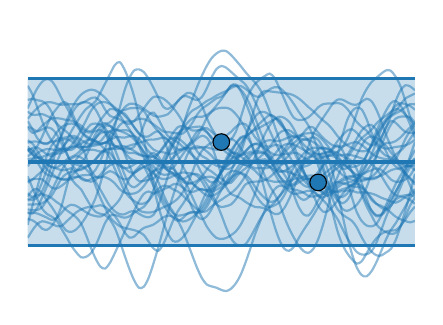
\begin{tikzpicture}
\begin{axis}[axis lines={none}, height={5cm}, width={6.5cm}, xmin={0}, xmax={1}, ymin={-1}, ymax={1}]
    \node at (0,-1) {};
    \node at (0,1) {};
    \node at (1,1) {};
    \node at (1,-1) {};
    \addplot[no markers, smooth, very thick, color={rgb,1:red,0.1216;green,0.4667;blue,0.7059}, name path={upper}]
        coordinates {
            (0.0,0.6198064213930023)
            (0.0125,0.6198064213930023)
            (0.025,0.6198064213930023)
            (0.0375,0.6198064213930023)
            (0.05,0.6198064213930023)
            (0.0625,0.6198064213930023)
            (0.075,0.6198064213930023)
            (0.0875,0.6198064213930023)
            (0.1,0.6198064213930023)
            (0.1125,0.6198064213930023)
            (0.125,0.6198064213930023)
            (0.1375,0.6198064213930023)
            (0.15,0.6198064213930023)
            (0.1625,0.6198064213930023)
            (0.175,0.6198064213930023)
            (0.1875,0.6198064213930023)
            (0.2,0.6198064213930023)
            (0.2125,0.6198064213930023)
            (0.225,0.6198064213930023)
            (0.2375,0.6198064213930023)
            (0.25,0.6198064213930023)
            (0.2625,0.6198064213930023)
            (0.275,0.6198064213930023)
            (0.2875,0.6198064213930023)
            (0.3,0.6198064213930023)
            (0.3125,0.6198064213930023)
            (0.325,0.6198064213930023)
            (0.3375,0.6198064213930023)
            (0.35,0.6198064213930023)
            (0.3625,0.6198064213930023)
            (0.375,0.6198064213930023)
            (0.3875,0.6198064213930023)
            (0.4,0.6198064213930023)
            (0.4125,0.6198064213930023)
            (0.425,0.6198064213930023)
            (0.4375,0.6198064213930023)
            (0.45,0.6198064213930023)
            (0.4625,0.6198064213930023)
            (0.475,0.6198064213930023)
            (0.4875,0.6198064213930023)
            (0.5,0.6198064213930023)
            (0.5125,0.6198064213930023)
            (0.525,0.6198064213930023)
            (0.5375,0.6198064213930023)
            (0.55,0.6198064213930023)
            (0.5625,0.6198064213930023)
            (0.575,0.6198064213930023)
            (0.5875,0.6198064213930023)
            (0.6,0.6198064213930023)
            (0.6125,0.6198064213930023)
            (0.625,0.6198064213930023)
            (0.6375,0.6198064213930023)
            (0.65,0.6198064213930023)
            (0.6625,0.6198064213930023)
            (0.675,0.6198064213930023)
            (0.6875,0.6198064213930023)
            (0.7,0.6198064213930023)
            (0.7125,0.6198064213930023)
            (0.725,0.6198064213930023)
            (0.7375,0.6198064213930023)
            (0.75,0.6198064213930023)
            (0.7625,0.6198064213930023)
            (0.775,0.6198064213930023)
            (0.7875,0.6198064213930023)
            (0.8,0.6198064213930023)
            (0.8125,0.6198064213930023)
            (0.825,0.6198064213930023)
            (0.8375,0.6198064213930023)
            (0.85,0.6198064213930023)
            (0.8625,0.6198064213930023)
            (0.875,0.6198064213930023)
            (0.8875,0.6198064213930023)
            (0.9,0.6198064213930023)
            (0.9125,0.6198064213930023)
            (0.925,0.6198064213930023)
            (0.9375,0.6198064213930023)
            (0.95,0.6198064213930023)
            (0.9625,0.6198064213930023)
            (0.975,0.6198064213930023)
            (0.9875,0.6198064213930023)
            (1.0,0.6198064213930023)
        }
        ;
    \addplot[no markers, smooth, very thick, color={rgb,1:red,0.1216;green,0.4667;blue,0.7059}, name path={lower}]
        coordinates {
            (0.0,-0.6198064213930023)
            (0.0125,-0.6198064213930023)
            (0.025,-0.6198064213930023)
            (0.0375,-0.6198064213930023)
            (0.05,-0.6198064213930023)
            (0.0625,-0.6198064213930023)
            (0.075,-0.6198064213930023)
            (0.0875,-0.6198064213930023)
            (0.1,-0.6198064213930023)
            (0.1125,-0.6198064213930023)
            (0.125,-0.6198064213930023)
            (0.1375,-0.6198064213930023)
            (0.15,-0.6198064213930023)
            (0.1625,-0.6198064213930023)
            (0.175,-0.6198064213930023)
            (0.1875,-0.6198064213930023)
            (0.2,-0.6198064213930023)
            (0.2125,-0.6198064213930023)
            (0.225,-0.6198064213930023)
            (0.2375,-0.6198064213930023)
            (0.25,-0.6198064213930023)
            (0.2625,-0.6198064213930023)
            (0.275,-0.6198064213930023)
            (0.2875,-0.6198064213930023)
            (0.3,-0.6198064213930023)
            (0.3125,-0.6198064213930023)
            (0.325,-0.6198064213930023)
            (0.3375,-0.6198064213930023)
            (0.35,-0.6198064213930023)
            (0.3625,-0.6198064213930023)
            (0.375,-0.6198064213930023)
            (0.3875,-0.6198064213930023)
            (0.4,-0.6198064213930023)
            (0.4125,-0.6198064213930023)
            (0.425,-0.6198064213930023)
            (0.4375,-0.6198064213930023)
            (0.45,-0.6198064213930023)
            (0.4625,-0.6198064213930023)
            (0.475,-0.6198064213930023)
            (0.4875,-0.6198064213930023)
            (0.5,-0.6198064213930023)
            (0.5125,-0.6198064213930023)
            (0.525,-0.6198064213930023)
            (0.5375,-0.6198064213930023)
            (0.55,-0.6198064213930023)
            (0.5625,-0.6198064213930023)
            (0.575,-0.6198064213930023)
            (0.5875,-0.6198064213930023)
            (0.6,-0.6198064213930023)
            (0.6125,-0.6198064213930023)
            (0.625,-0.6198064213930023)
            (0.6375,-0.6198064213930023)
            (0.65,-0.6198064213930023)
            (0.6625,-0.6198064213930023)
            (0.675,-0.6198064213930023)
            (0.6875,-0.6198064213930023)
            (0.7,-0.6198064213930023)
            (0.7125,-0.6198064213930023)
            (0.725,-0.6198064213930023)
            (0.7375,-0.6198064213930023)
            (0.75,-0.6198064213930023)
            (0.7625,-0.6198064213930023)
            (0.775,-0.6198064213930023)
            (0.7875,-0.6198064213930023)
            (0.8,-0.6198064213930023)
            (0.8125,-0.6198064213930023)
            (0.825,-0.6198064213930023)
            (0.8375,-0.6198064213930023)
            (0.85,-0.6198064213930023)
            (0.8625,-0.6198064213930023)
            (0.875,-0.6198064213930023)
            (0.8875,-0.6198064213930023)
            (0.9,-0.6198064213930023)
            (0.9125,-0.6198064213930023)
            (0.925,-0.6198064213930023)
            (0.9375,-0.6198064213930023)
            (0.95,-0.6198064213930023)
            (0.9625,-0.6198064213930023)
            (0.975,-0.6198064213930023)
            (0.9875,-0.6198064213930023)
            (1.0,-0.6198064213930023)
        }
        ;
    \addplot[color={rgb,1:red,0.1216;green,0.4667;blue,0.7059}, opacity={0.25}]
        fill between [of = upper and lower]
        ;
    \draw[ultra thick, color={rgb,1:red,0.1216;green,0.4667;blue,0.7059}] ({rel axis cs:1,0}|-{axis cs:0,0}) -- ({rel axis cs:0,0}|-{axis cs:0,0});
    \addplot[no markers, smooth, thick, color={rgb,1:red,0.1216;green,0.4667;blue,0.7059}, opacity={0.5}]
        coordinates {
            (0.0,0.46305457253556626)
            (0.0125,0.47028438294516756)
            (0.025,0.4607105971778673)
            (0.0375,0.45348962182474833)
            (0.05,0.42728212560616824)
            (0.0625,0.3688272761222826)
            (0.075,0.2861558773993253)
            (0.0875,0.1835964509360369)
            (0.1,0.07758328200661428)
            (0.1125,-0.010389681095359052)
            (0.125,-0.0557081645779113)
            (0.1375,-0.05706238286573637)
            (0.15,-0.03802998049931)
            (0.1625,-0.012960371653227028)
            (0.175,0.02339110240165655)
            (0.1875,0.06724060919401285)
            (0.2,0.09560053597193445)
            (0.2125,0.10005706513904698)
            (0.225,0.09963935081741737)
            (0.2375,0.101322594923364)
            (0.25,0.09574296324318654)
            (0.2625,0.0988946085710455)
            (0.275,0.11497591695844238)
            (0.2875,0.1793305784676947)
            (0.3,0.2753301249775372)
            (0.3125,0.3510708184703537)
            (0.325,0.3688081387631436)
            (0.3375,0.3205933183571491)
            (0.35,0.250894791558468)
            (0.3625,0.19391076054125517)
            (0.375,0.16992099665954463)
            (0.3875,0.14790115812332974)
            (0.4,0.11629150747224322)
            (0.4125,0.08668476674378722)
            (0.425,0.052454506206027936)
            (0.4375,0.02159759373022147)
            (0.45,-0.014494692269275055)
            (0.4625,-0.046998322722103955)
            (0.475,-0.06861649761565053)
            (0.4875,-0.09747243645260237)
            (0.5,-0.12174274470316762)
            (0.5125,-0.1491557878012935)
            (0.525,-0.1525985561797283)
            (0.5375,-0.1125143327812058)
            (0.55,-0.07390256548235694)
            (0.5625,-0.04566476163067383)
            (0.575,-0.019676113890765946)
            (0.5875,0.0094253679556406)
            (0.6,0.038982523616113006)
            (0.6125,0.07305166095193896)
            (0.625,0.11040569609881253)
            (0.6375,0.12753318634359734)
            (0.65,0.12327280280199604)
            (0.6625,0.09809439609948886)
            (0.675,0.048154612532929006)
            (0.6875,-0.01594192924686807)
            (0.7,-0.08434132099579834)
            (0.7125,-0.13289177616308734)
            (0.725,-0.16829536995771285)
            (0.7375,-0.18365969034017265)
            (0.75,-0.19966149045408174)
            (0.7625,-0.2286488450925192)
            (0.775,-0.24959968171410743)
            (0.7875,-0.22933514792302293)
            (0.8,-0.18798239806025047)
            (0.8125,-0.1623038142846837)
            (0.825,-0.1515258393433178)
            (0.8375,-0.1441734262006973)
            (0.85,-0.1250092116232625)
            (0.8625,-0.09727088747409654)
            (0.875,-0.07307981815729453)
            (0.8875,-0.0597609649634399)
            (0.9,-0.04553367035120032)
            (0.9125,-0.056541124176529525)
            (0.925,-0.08716622214291082)
            (0.9375,-0.12729308103947026)
            (0.95,-0.1448011938673927)
            (0.9625,-0.14246555215792756)
            (0.975,-0.12910443668077484)
            (0.9875,-0.09807530087854183)
            (1.0,-0.03986449643477344)
        }
        ;
    \addplot[no markers, smooth, thick, color={rgb,1:red,0.1216;green,0.4667;blue,0.7059}, opacity={0.5}]
        coordinates {
            (0.0,-0.46428788727528664)
            (0.0125,-0.3213457544959877)
            (0.025,-0.1852458079069437)
            (0.0375,-0.057821300925710944)
            (0.05,0.05078254507665389)
            (0.0625,0.12785518535010063)
            (0.075,0.16944613965871402)
            (0.0875,0.17992756010517572)
            (0.1,0.18577297332037943)
            (0.1125,0.1959703704373607)
            (0.125,0.19095062865464396)
            (0.1375,0.16597976241065324)
            (0.15,0.1447051148187759)
            (0.1625,0.13270647148071082)
            (0.175,0.1348554365278997)
            (0.1875,0.13510851536557666)
            (0.2,0.14605727460948773)
            (0.2125,0.13789478735510796)
            (0.225,0.12067242573457528)
            (0.2375,0.10640787962877181)
            (0.25,0.10923369950502439)
            (0.2625,0.1237078161869972)
            (0.275,0.13387552374608075)
            (0.2875,0.14485937285407094)
            (0.3,0.15527072936639139)
            (0.3125,0.16795641745207313)
            (0.325,0.16808926053890505)
            (0.3375,0.17464382728177238)
            (0.35,0.18276033896219623)
            (0.3625,0.16658460121044324)
            (0.375,0.12582048260866271)
            (0.3875,0.09613248431585102)
            (0.4,0.09378652722118586)
            (0.4125,0.11053486780644707)
            (0.425,0.14020497357330497)
            (0.4375,0.1758641109296083)
            (0.45,0.19678706714989527)
            (0.4625,0.18204104960383433)
            (0.475,0.12367193724818894)
            (0.4875,0.019862903497726077)
            (0.5,-0.08865162077310965)
            (0.5125,-0.18533223857703765)
            (0.525,-0.23578395801232074)
            (0.5375,-0.25058645881298264)
            (0.55,-0.26843671359891363)
            (0.5625,-0.2948809170335332)
            (0.575,-0.3153061631598945)
            (0.5875,-0.33224234279488957)
            (0.6,-0.3348709591466116)
            (0.6125,-0.34430991643774544)
            (0.625,-0.3626188202779805)
            (0.6375,-0.3839242558553632)
            (0.65,-0.38034427136362686)
            (0.6625,-0.34107701729457574)
            (0.675,-0.27305312809935495)
            (0.6875,-0.18935706230140084)
            (0.7,-0.10234725526321486)
            (0.7125,0.00045987528693074213)
            (0.725,0.11984704892133799)
            (0.7375,0.21081138736118865)
            (0.75,0.2751126473721614)
            (0.7625,0.32862650783243413)
            (0.775,0.38136684938300025)
            (0.7875,0.4338284057634397)
            (0.8,0.4650820953290081)
            (0.8125,0.46495603923586293)
            (0.825,0.4469430839303263)
            (0.8375,0.43016783664605707)
            (0.85,0.4280674675921127)
            (0.8625,0.4483927886169613)
            (0.875,0.47176108945538475)
            (0.8875,0.4541950021243955)
            (0.9,0.39375253308154484)
            (0.9125,0.3056390540894031)
            (0.925,0.20799130284713693)
            (0.9375,0.11927897650906832)
            (0.95,0.04241184919500316)
            (0.9625,-0.007622728003104103)
            (0.975,-0.02901007355977709)
            (0.9875,-0.02966249474410153)
            (1.0,-0.008023017157779767)
        }
        ;
    \addplot[no markers, smooth, thick, color={rgb,1:red,0.1216;green,0.4667;blue,0.7059}, opacity={0.5}]
        coordinates {
            (0.0,0.25851581355535835)
            (0.0125,0.21860322069957117)
            (0.025,0.23194039744024442)
            (0.0375,0.27112893757263834)
            (0.05,0.30071845677744785)
            (0.0625,0.325977356611455)
            (0.075,0.32741178313980374)
            (0.0875,0.32278114994238055)
            (0.1,0.3141702491093429)
            (0.1125,0.3089564947351909)
            (0.125,0.2940390588826041)
            (0.1375,0.27311984761774305)
            (0.15,0.239686785680621)
            (0.1625,0.2301746838632721)
            (0.175,0.2573789185092609)
            (0.1875,0.2835204675722094)
            (0.2,0.2898410987674376)
            (0.2125,0.27137781757303425)
            (0.225,0.24745939584841292)
            (0.2375,0.23357461569674695)
            (0.25,0.2190563291063412)
            (0.2625,0.2004499750060921)
            (0.275,0.16983564827980394)
            (0.2875,0.12459043857888841)
            (0.3,0.07693116434345162)
            (0.3125,0.035260336553412645)
            (0.325,-0.00226023611499642)
            (0.3375,-0.021409335224061056)
            (0.35,-0.03850398884110251)
            (0.3625,-0.06061210674351323)
            (0.375,-0.08171967024917072)
            (0.3875,-0.12382840837077486)
            (0.4,-0.18125448413273665)
            (0.4125,-0.25356934249159624)
            (0.425,-0.3410108047797957)
            (0.4375,-0.40061538596558877)
            (0.45,-0.42299988989931764)
            (0.4625,-0.40162781514061985)
            (0.475,-0.34873514161848507)
            (0.4875,-0.27335714431026265)
            (0.5,-0.20755372532681093)
            (0.5125,-0.15178579961938993)
            (0.525,-0.11313246763702262)
            (0.5375,-0.08958867431640108)
            (0.55,-0.08205384669608137)
            (0.5625,-0.11219917701359691)
            (0.575,-0.17036668687896286)
            (0.5875,-0.23659492341550342)
            (0.6,-0.2899906375746055)
            (0.6125,-0.3241664648371033)
            (0.625,-0.33378765076985667)
            (0.6375,-0.32018011351467324)
            (0.65,-0.29781217728984677)
            (0.6625,-0.2453249735052363)
            (0.675,-0.17454169197608635)
            (0.6875,-0.10947784044354378)
            (0.7,-0.06023075390237954)
            (0.7125,-0.033552404449240174)
            (0.725,-0.022460675958383747)
            (0.7375,0.0029772761970070813)
            (0.75,0.03311493520148072)
            (0.7625,0.042907186845115464)
            (0.775,0.04929010193501296)
            (0.7875,0.0459254122029944)
            (0.8,0.029458598634812663)
            (0.8125,-0.0016647442715152325)
            (0.825,-0.03819389630158464)
            (0.8375,-0.0660820198370484)
            (0.85,-0.1224136296125345)
            (0.8625,-0.21698548251622776)
            (0.875,-0.2992859606168876)
            (0.8875,-0.35581278518749426)
            (0.9,-0.3925251699297761)
            (0.9125,-0.3883442436899143)
            (0.925,-0.3409500589280415)
            (0.9375,-0.27595542603747697)
            (0.95,-0.21798575489425037)
            (0.9625,-0.1516986150862594)
            (0.975,-0.06040725219160424)
            (0.9875,0.046918225897317395)
            (1.0,0.15057207780047405)
        }
        ;
    \addplot[no markers, smooth, thick, color={rgb,1:red,0.1216;green,0.4667;blue,0.7059}, opacity={0.5}]
        coordinates {
            (0.0,-0.23008816344186106)
            (0.0125,-0.2577110012962528)
            (0.025,-0.22880238565462563)
            (0.0375,-0.14780857822614876)
            (0.05,-0.051009561237610086)
            (0.0625,0.03719398729436228)
            (0.075,0.08800904371017672)
            (0.0875,0.10078302133671228)
            (0.1,0.09448996950079783)
            (0.1125,0.09129953760333626)
            (0.125,0.1161424278906519)
            (0.1375,0.17464543822017387)
            (0.15,0.23553736667535455)
            (0.1625,0.2796502072787637)
            (0.175,0.28737569493103843)
            (0.1875,0.27903304082182284)
            (0.2,0.2525993007730641)
            (0.2125,0.18427428210878607)
            (0.225,0.09594451759780026)
            (0.2375,0.004626114676674028)
            (0.25,-0.08999628301951296)
            (0.2625,-0.1663649674606581)
            (0.275,-0.1859840026335454)
            (0.2875,-0.16234537353940517)
            (0.3,-0.12886016607337486)
            (0.3125,-0.096496451912165)
            (0.325,-0.06565876019507205)
            (0.3375,-0.05164909219325721)
            (0.35,-0.036991618790672046)
            (0.3625,-0.0340565627008504)
            (0.375,-0.049089383322269343)
            (0.3875,-0.08541074660132432)
            (0.4,-0.1273797694368968)
            (0.4125,-0.15116529795994627)
            (0.425,-0.15944488299846907)
            (0.4375,-0.18519055941015092)
            (0.45,-0.22113977570117507)
            (0.4625,-0.24701933102913629)
            (0.475,-0.2501775552594254)
            (0.4875,-0.23569828018351566)
            (0.5,-0.20225046456044263)
            (0.5125,-0.16906309622059304)
            (0.525,-0.11804580053645455)
            (0.5375,-0.05891593307394825)
            (0.55,-0.005543457541793145)
            (0.5625,0.03586819217732367)
            (0.575,0.06286583623569063)
            (0.5875,0.06888032215204824)
            (0.6,0.06928859540932082)
            (0.6125,0.070048033386935)
            (0.625,0.03842402334211707)
            (0.6375,-0.032199145153266)
            (0.65,-0.10451768055263275)
            (0.6625,-0.15746837513908737)
            (0.675,-0.1768228495828187)
            (0.6875,-0.1709347404935195)
            (0.7,-0.14966552558934715)
            (0.7125,-0.1294832972611853)
            (0.725,-0.12261787663467646)
            (0.7375,-0.10885682560222322)
            (0.75,-0.07213673000427989)
            (0.7625,-0.022387898199493078)
            (0.775,0.005343570514595451)
            (0.7875,0.00457729344211812)
            (0.8,-0.020587671286955298)
            (0.8125,-0.04816572554409732)
            (0.825,-0.043729266693238164)
            (0.8375,-0.010326408715250618)
            (0.85,0.05688490428921813)
            (0.8625,0.12485570477233845)
            (0.875,0.17726411291631092)
            (0.8875,0.1918833805439719)
            (0.9,0.17991960935337245)
            (0.9125,0.15941322397992735)
            (0.925,0.12164981367018114)
            (0.9375,0.07451726956380905)
            (0.95,0.028028375841376053)
            (0.9625,-0.004988790307701452)
            (0.975,-0.01798106562544914)
            (0.9875,-0.027549105544791196)
            (1.0,-0.02555202863272954)
        }
        ;
    \addplot[no markers, smooth, thick, color={rgb,1:red,0.1216;green,0.4667;blue,0.7059}, opacity={0.5}]
        coordinates {
            (0.0,-0.10413036670368635)
            (0.0125,-0.19080223969327684)
            (0.025,-0.27473527848096563)
            (0.0375,-0.34530816028455696)
            (0.05,-0.38420543666415546)
            (0.0625,-0.4045333447713484)
            (0.075,-0.43337257522537936)
            (0.0875,-0.49583806865239904)
            (0.1,-0.5554460913677431)
            (0.1125,-0.6193023633712301)
            (0.125,-0.6674657555456514)
            (0.1375,-0.7055210877963812)
            (0.15,-0.704007369133143)
            (0.1625,-0.6778138981086238)
            (0.175,-0.6209725944049561)
            (0.1875,-0.5373040835681302)
            (0.2,-0.4501965349074897)
            (0.2125,-0.3980914697504373)
            (0.225,-0.39151735368934315)
            (0.2375,-0.40279480066246043)
            (0.25,-0.411878045715026)
            (0.2625,-0.4020640578104902)
            (0.275,-0.3750322267300074)
            (0.2875,-0.35153508169703707)
            (0.3,-0.3307318356096615)
            (0.3125,-0.28317834953794935)
            (0.325,-0.2042840376668968)
            (0.3375,-0.11309094446786955)
            (0.35,-0.024192757341355058)
            (0.3625,0.05376539440821445)
            (0.375,0.12656390123262382)
            (0.3875,0.19450352709695642)
            (0.4,0.24692977116454698)
            (0.4125,0.2931923129069142)
            (0.425,0.32615961393683895)
            (0.4375,0.33835726975170544)
            (0.45,0.3380091334599469)
            (0.4625,0.35173803470662934)
            (0.475,0.3790810360398524)
            (0.4875,0.42150970098395185)
            (0.5,0.466822610667487)
            (0.5125,0.5207715883467375)
            (0.525,0.5660590937915739)
            (0.5375,0.569092205138048)
            (0.55,0.5406117782571895)
            (0.5625,0.49214182421195446)
            (0.575,0.4193642821296696)
            (0.5875,0.32910319693308726)
            (0.6,0.2349676778851878)
            (0.6125,0.14804194109245067)
            (0.625,0.06348453324576023)
            (0.6375,0.004617052670573864)
            (0.65,-0.016564216427645554)
            (0.6625,-0.011356478295258526)
            (0.675,-0.00315249999205236)
            (0.6875,0.0012011675748621524)
            (0.7,-0.027305645489660187)
            (0.7125,-0.08160743702834758)
            (0.725,-0.12438076845001024)
            (0.7375,-0.1276824717912562)
            (0.75,-0.0933680831157823)
            (0.7625,-0.026814090025548697)
            (0.775,0.04325533272008816)
            (0.7875,0.0973864977350346)
            (0.8,0.1248258124641326)
            (0.8125,0.09012370473143774)
            (0.825,0.009161099353381707)
            (0.8375,-0.07031136435125188)
            (0.85,-0.149155511587161)
            (0.8625,-0.241214425845225)
            (0.875,-0.3264221324840802)
            (0.8875,-0.39419102655444443)
            (0.9,-0.4605219701906045)
            (0.9125,-0.4968599751245701)
            (0.925,-0.5187159807069315)
            (0.9375,-0.530998107727672)
            (0.95,-0.5255938873382417)
            (0.9625,-0.4792405584474534)
            (0.975,-0.4060882039674933)
            (0.9875,-0.3207567138771029)
            (1.0,-0.26567469134666044)
        }
        ;
    \addplot[no markers, smooth, thick, color={rgb,1:red,0.1216;green,0.4667;blue,0.7059}, opacity={0.5}]
        coordinates {
            (0.0,-0.1393812217296162)
            (0.0125,-0.12575894659597894)
            (0.025,-0.12343193427837748)
            (0.0375,-0.1273047526240373)
            (0.05,-0.1577743785415941)
            (0.0625,-0.18938012314329877)
            (0.075,-0.19472147753201455)
            (0.0875,-0.17476922579170884)
            (0.1,-0.1455891996989187)
            (0.1125,-0.10245749686456046)
            (0.125,-0.06623669922901367)
            (0.1375,-0.025637652952121535)
            (0.15,0.041295399436209385)
            (0.1625,0.11569506235838618)
            (0.175,0.1795660356873079)
            (0.1875,0.21483552282556143)
            (0.2,0.22641662505435564)
            (0.2125,0.22611983233877359)
            (0.225,0.19915285134911373)
            (0.2375,0.14631646829484127)
            (0.25,0.06538587390577791)
            (0.2625,-0.023414242420980617)
            (0.275,-0.10155298166845772)
            (0.2875,-0.13985408632582189)
            (0.3,-0.13923181667678305)
            (0.3125,-0.12930202278047578)
            (0.325,-0.12009390152098928)
            (0.3375,-0.07882119215247245)
            (0.35,-0.015028386502739266)
            (0.3625,0.061755317067788126)
            (0.375,0.13276836674813206)
            (0.3875,0.19127366189224998)
            (0.4,0.26855552573449776)
            (0.4125,0.3421502571667553)
            (0.425,0.38331241592276016)
            (0.4375,0.40349264630355625)
            (0.45,0.42823812759582847)
            (0.4625,0.4552240646848931)
            (0.475,0.4729715008199965)
            (0.4875,0.4955983115064812)
            (0.5,0.5135951830283463)
            (0.5125,0.5291980382520642)
            (0.525,0.5508386780545529)
            (0.5375,0.5663515754520946)
            (0.55,0.5663542848341847)
            (0.5625,0.5455447120085246)
            (0.575,0.515254654415423)
            (0.5875,0.49033031493001566)
            (0.6,0.4885467493135342)
            (0.6125,0.5139774435358574)
            (0.625,0.54210084247563)
            (0.6375,0.5575316300783917)
            (0.65,0.5539634476509405)
            (0.6625,0.5219345964558534)
            (0.675,0.48190061218450525)
            (0.6875,0.43185444733708983)
            (0.7,0.3746160140193789)
            (0.7125,0.32615188511572507)
            (0.725,0.27217636693417424)
            (0.7375,0.19150965672129172)
            (0.75,0.08891087569429669)
            (0.7625,-0.025060615827294092)
            (0.775,-0.15166852654653695)
            (0.7875,-0.2745039467383329)
            (0.8,-0.3489323123470604)
            (0.8125,-0.387565820707712)
            (0.825,-0.41213466263162635)
            (0.8375,-0.43614255259996765)
            (0.85,-0.48512343194431706)
            (0.8625,-0.5578323553103015)
            (0.875,-0.6167167111463588)
            (0.8875,-0.6628367782559127)
            (0.9,-0.6908057431204546)
            (0.9125,-0.6932566020318032)
            (0.925,-0.6709482791120364)
            (0.9375,-0.6448435864357821)
            (0.95,-0.5801157741056336)
            (0.9625,-0.4786250968170996)
            (0.975,-0.35922130088870885)
            (0.9875,-0.22726097892171537)
            (1.0,-0.08563883289451606)
        }
        ;
    \addplot[no markers, smooth, thick, color={rgb,1:red,0.1216;green,0.4667;blue,0.7059}, opacity={0.5}]
        coordinates {
            (0.0,0.14536587184926705)
            (0.0125,0.15322749821211165)
            (0.025,0.15299527348574318)
            (0.0375,0.14264247274800604)
            (0.05,0.14147276255182853)
            (0.0625,0.15355506317684478)
            (0.075,0.15600311578237275)
            (0.0875,0.16620293270297912)
            (0.1,0.1713495658679258)
            (0.1125,0.15816605132149775)
            (0.125,0.12482691555087602)
            (0.1375,0.09720053588447589)
            (0.15,0.09000400655489964)
            (0.1625,0.13434549402715143)
            (0.175,0.20787310859862668)
            (0.1875,0.2601084839219124)
            (0.2,0.28262402617150123)
            (0.2125,0.29668026528920843)
            (0.225,0.3330752448899809)
            (0.2375,0.3671780214491677)
            (0.25,0.36184093939217443)
            (0.2625,0.3167849573587059)
            (0.275,0.2601290905536253)
            (0.2875,0.21157118330345573)
            (0.3,0.19162536784314793)
            (0.3125,0.1925489355574019)
            (0.325,0.21788389086848092)
            (0.3375,0.22938261676607966)
            (0.35,0.17911082195323738)
            (0.3625,0.08356116283029498)
            (0.375,-0.02227848019551686)
            (0.3875,-0.10372998936893917)
            (0.4,-0.12714447144378316)
            (0.4125,-0.1067197999659576)
            (0.425,-0.08705791688550071)
            (0.4375,-0.08855679188735661)
            (0.45,-0.11134061922943203)
            (0.4625,-0.16372326320345024)
            (0.475,-0.22844167882419986)
            (0.4875,-0.3033228710363365)
            (0.5,-0.38961835822998275)
            (0.5125,-0.48544107868848047)
            (0.525,-0.5650275817289242)
            (0.5375,-0.6080984021802307)
            (0.55,-0.6208536035838994)
            (0.5625,-0.6085125942274358)
            (0.575,-0.5565635463564268)
            (0.5875,-0.490911449857044)
            (0.6,-0.423945409242767)
            (0.6125,-0.36812376634188904)
            (0.625,-0.33298130613740046)
            (0.6375,-0.29849388873485894)
            (0.65,-0.25600143161602373)
            (0.6625,-0.19140291058828238)
            (0.675,-0.10659940514161369)
            (0.6875,-0.035240943439402136)
            (0.7,0.020837414709229753)
            (0.7125,0.06371592129769033)
            (0.725,0.09472303977177106)
            (0.7375,0.10697519785595196)
            (0.75,0.10812402613310014)
            (0.7625,0.10099460171686885)
            (0.775,0.10208299978578299)
            (0.7875,0.08016207349786127)
            (0.8,0.0472527039244403)
            (0.8125,0.0016903242042611106)
            (0.825,-0.02588896569190307)
            (0.8375,-0.034459919007942263)
            (0.85,-0.027849845560002428)
            (0.8625,-0.0039053913878736935)
            (0.875,0.04863248108756512)
            (0.8875,0.1351335565186239)
            (0.9,0.22793190456261353)
            (0.9125,0.30871705480719785)
            (0.925,0.38122622821654084)
            (0.9375,0.43858343655663684)
            (0.95,0.45562885664955843)
            (0.9625,0.42193147590149777)
            (0.975,0.35913330725911385)
            (0.9875,0.2803599057149603)
            (1.0,0.17681953958750493)
        }
        ;
    \addplot[no markers, smooth, thick, color={rgb,1:red,0.1216;green,0.4667;blue,0.7059}, opacity={0.5}]
        coordinates {
            (0.0,0.3215223023002469)
            (0.0125,0.36600113875391266)
            (0.025,0.40301596321706207)
            (0.0375,0.4314673276005611)
            (0.05,0.44537172360632304)
            (0.0625,0.44466200704792724)
            (0.075,0.43422110869336833)
            (0.0875,0.42776972180409173)
            (0.1,0.4295228264973817)
            (0.1125,0.43136849106924635)
            (0.125,0.4304268452669429)
            (0.1375,0.43694217419215714)
            (0.15,0.4544293567858089)
            (0.1625,0.4749722454325684)
            (0.175,0.48039630215761836)
            (0.1875,0.45234832903173794)
            (0.2,0.391006437421291)
            (0.2125,0.3452254051465144)
            (0.225,0.33209540326899284)
            (0.2375,0.31884331098184165)
            (0.25,0.2958756331738433)
            (0.2625,0.2835460567612009)
            (0.275,0.3067376083993798)
            (0.2875,0.3515331280200237)
            (0.3,0.4000906328547078)
            (0.3125,0.449741574265104)
            (0.325,0.485425441217221)
            (0.3375,0.48593101951529893)
            (0.35,0.4734584922378752)
            (0.3625,0.444671711996285)
            (0.375,0.40548796321358804)
            (0.3875,0.3594907762878496)
            (0.4,0.3009166967292951)
            (0.4125,0.22909908795409498)
            (0.425,0.15193300695011433)
            (0.4375,0.0802242595776057)
            (0.45,0.04585326488030096)
            (0.4625,0.02637143475954301)
            (0.475,-0.0029495871193441488)
            (0.4875,-0.026142388677419227)
            (0.5,-0.0358332329759578)
            (0.5125,-0.05120046052009373)
            (0.525,-0.04401793426643665)
            (0.5375,-0.006966897691324414)
            (0.55,0.07082995636469418)
            (0.5625,0.17744213487430205)
            (0.575,0.2962414779573753)
            (0.5875,0.4173087948650079)
            (0.6,0.5028784401739669)
            (0.6125,0.5300280095152189)
            (0.625,0.5267139267320562)
            (0.6375,0.5222812218773013)
            (0.65,0.5177324626844775)
            (0.6625,0.5141417812200485)
            (0.675,0.5085889350964823)
            (0.6875,0.4962076657026762)
            (0.7,0.474111101196661)
            (0.7125,0.4434905680438788)
            (0.725,0.40954219305961903)
            (0.7375,0.37967985697760903)
            (0.75,0.3445807432063752)
            (0.7625,0.31136071111994224)
            (0.775,0.2826954947601579)
            (0.7875,0.24327783574632528)
            (0.8,0.19471050037723145)
            (0.8125,0.15559010975061233)
            (0.825,0.12682705054732268)
            (0.8375,0.1051181777645481)
            (0.85,0.08904721509763198)
            (0.8625,0.08172970552912052)
            (0.875,0.08497362564092312)
            (0.8875,0.12021729019957492)
            (0.9,0.19831331697529242)
            (0.9125,0.2712972655531311)
            (0.925,0.31866363224017)
            (0.9375,0.34620398863757834)
            (0.95,0.37970807472957824)
            (0.9625,0.42860331797828144)
            (0.975,0.47360406996497384)
            (0.9875,0.4929172377566296)
            (1.0,0.5113190185484385)
        }
        ;
    \addplot[no markers, smooth, thick, color={rgb,1:red,0.1216;green,0.4667;blue,0.7059}, opacity={0.5}]
        coordinates {
            (0.0,-0.03054225793464809)
            (0.0125,0.022081122500137402)
            (0.025,0.06722534670450557)
            (0.0375,0.08750754323258057)
            (0.05,0.09778934174913272)
            (0.0625,0.0952320417540714)
            (0.075,0.08804024134583316)
            (0.0875,0.08417565984773408)
            (0.1,0.0901019407329108)
            (0.1125,0.10647521361891721)
            (0.125,0.12387997543413484)
            (0.1375,0.13706919224161307)
            (0.15,0.1595514318404564)
            (0.1625,0.1706840095530482)
            (0.175,0.15646220895650395)
            (0.1875,0.1321630289858299)
            (0.2,0.08853754095344735)
            (0.2125,0.027972587286884683)
            (0.225,-0.04853956900844364)
            (0.2375,-0.13097766917749698)
            (0.25,-0.21219062767649158)
            (0.2625,-0.25934234983268667)
            (0.275,-0.2871391777022636)
            (0.2875,-0.3074409168968967)
            (0.3,-0.3063564317709992)
            (0.3125,-0.28507516870881555)
            (0.325,-0.2375062843286988)
            (0.3375,-0.19825953065007693)
            (0.35,-0.17422667977598366)
            (0.3625,-0.17911596930536147)
            (0.375,-0.20077882113734516)
            (0.3875,-0.21675107997705623)
            (0.4,-0.2458392707713178)
            (0.4125,-0.2831437333561512)
            (0.425,-0.3174494984510335)
            (0.4375,-0.35059777336604087)
            (0.45,-0.36854757686977224)
            (0.4625,-0.361999089711998)
            (0.475,-0.32818339839731364)
            (0.4875,-0.3006462671795676)
            (0.5,-0.27844991279055353)
            (0.5125,-0.2539683485079886)
            (0.525,-0.2301905932924959)
            (0.5375,-0.1985460984746674)
            (0.55,-0.15443319049938167)
            (0.5625,-0.09969217615835656)
            (0.575,-0.029949478535401107)
            (0.5875,0.04081008655065418)
            (0.6,0.1259243212358609)
            (0.6125,0.2103100710704732)
            (0.625,0.27425342949928055)
            (0.6375,0.31991465811891995)
            (0.65,0.3390257382265144)
            (0.6625,0.32945841975608775)
            (0.675,0.3007085054214226)
            (0.6875,0.24616107464842404)
            (0.7,0.17143787187522605)
            (0.7125,0.09885774910702261)
            (0.725,0.061889826219041606)
            (0.7375,0.04202405966737147)
            (0.75,0.01360685064455217)
            (0.7625,-0.06244550197265388)
            (0.775,-0.14881162896091185)
            (0.7875,-0.2132311314831925)
            (0.8,-0.2544522903818717)
            (0.8125,-0.25814719861255847)
            (0.825,-0.23304341896506905)
            (0.8375,-0.1844218602713221)
            (0.85,-0.12656937118634026)
            (0.8625,-0.06804406447262473)
            (0.875,-0.012783444747005695)
            (0.8875,0.03486752671248276)
            (0.9,0.0769628880245681)
            (0.9125,0.11533972366755305)
            (0.925,0.1418965530204817)
            (0.9375,0.14457226686875274)
            (0.95,0.15708145148318708)
            (0.9625,0.18441829054466474)
            (0.975,0.22240577661831215)
            (0.9875,0.2585437809239896)
            (1.0,0.29167542718907885)
        }
        ;
    \addplot[no markers, smooth, thick, color={rgb,1:red,0.1216;green,0.4667;blue,0.7059}, opacity={0.5}]
        coordinates {
            (0.0,0.30649762526792346)
            (0.0125,0.2448752874061577)
            (0.025,0.17829713132572914)
            (0.0375,0.1431238367168278)
            (0.05,0.13466361360605428)
            (0.0625,0.16676349975866084)
            (0.075,0.22184802565404815)
            (0.0875,0.261563206020695)
            (0.1,0.2798598351435089)
            (0.1125,0.2876710110679291)
            (0.125,0.28009735714139916)
            (0.1375,0.25247712313392057)
            (0.15,0.22579807879002697)
            (0.1625,0.22144173207540702)
            (0.175,0.23203066385624907)
            (0.1875,0.2384344891848729)
            (0.2,0.21741745911470634)
            (0.2125,0.16500218850233986)
            (0.225,0.12322598212526381)
            (0.2375,0.10693041395086357)
            (0.25,0.0849495991037536)
            (0.2625,0.06829578170306833)
            (0.275,0.06931961278011285)
            (0.2875,0.05554127591757286)
            (0.3,0.044479252013279666)
            (0.3125,0.04681409332930808)
            (0.325,0.03851238004345438)
            (0.3375,0.018276364312431622)
            (0.35,-0.022716489015063346)
            (0.3625,-0.050272230252332795)
            (0.375,-0.04101325096502869)
            (0.3875,0.005575298971066842)
            (0.4,0.05666343630994273)
            (0.4125,0.1096096543021849)
            (0.425,0.17275621346240558)
            (0.4375,0.22824494857752234)
            (0.45,0.24326011032321723)
            (0.4625,0.22325056868759374)
            (0.475,0.1857079277118524)
            (0.4875,0.14859438938761657)
            (0.5,0.12392299900516399)
            (0.5125,0.10271921828547738)
            (0.525,0.075308320977222)
            (0.5375,0.06020614585126429)
            (0.55,0.04368541845449475)
            (0.5625,0.014736552911093003)
            (0.575,-0.025377939841969458)
            (0.5875,-0.044324959416130516)
            (0.6,-0.04192353899442216)
            (0.6125,-0.04549458771792518)
            (0.625,-0.03632929544670603)
            (0.6375,-0.009980798042441197)
            (0.65,0.0403339986630179)
            (0.6625,0.09188701886921777)
            (0.675,0.14578270493925177)
            (0.6875,0.18047536966561867)
            (0.7,0.1917275020542973)
            (0.7125,0.19691948657371844)
            (0.725,0.15965260355474173)
            (0.7375,0.07895023245770151)
            (0.75,-0.024177365442145545)
            (0.7625,-0.12977844800437288)
            (0.775,-0.24167782987219838)
            (0.7875,-0.37529999676812886)
            (0.8,-0.512179591048028)
            (0.8125,-0.6112220928691741)
            (0.825,-0.6753588081692846)
            (0.8375,-0.7217578683740683)
            (0.85,-0.7531252370646018)
            (0.8625,-0.7354473840840455)
            (0.875,-0.6772992617719282)
            (0.8875,-0.6165096062456443)
            (0.9,-0.566232942329938)
            (0.9125,-0.5337002286142136)
            (0.925,-0.5155561818950821)
            (0.9375,-0.5068733442611214)
            (0.95,-0.5045357685357886)
            (0.9625,-0.4736039226672582)
            (0.975,-0.4260721204009789)
            (0.9875,-0.37242092022756856)
            (1.0,-0.32977048878174275)
        }
        ;
    \addplot[no markers, smooth, thick, color={rgb,1:red,0.1216;green,0.4667;blue,0.7059}, opacity={0.5}]
        coordinates {
            (0.0,0.3998607301278429)
            (0.0125,0.47979391305014585)
            (0.025,0.5499232560164967)
            (0.0375,0.5984996318409178)
            (0.05,0.618773000092868)
            (0.0625,0.6023932268370419)
            (0.075,0.5475404033755541)
            (0.0875,0.4747746575567777)
            (0.1,0.41076588853756435)
            (0.1125,0.3462854058178571)
            (0.125,0.2815851416598813)
            (0.1375,0.22565849272841984)
            (0.15,0.18956867164601965)
            (0.1625,0.16425002275526346)
            (0.175,0.14616991012423955)
            (0.1875,0.15535674956592396)
            (0.2,0.19850439130953498)
            (0.2125,0.2318223282685624)
            (0.225,0.2390536574991914)
            (0.2375,0.23581507253318745)
            (0.25,0.23816334715531867)
            (0.2625,0.23235210948314988)
            (0.275,0.19844196702292338)
            (0.2875,0.1380441145414266)
            (0.3,0.07402691510391948)
            (0.3125,0.0049862302981036515)
            (0.325,-0.07041609329754844)
            (0.3375,-0.14732790592600523)
            (0.35,-0.23616903853805654)
            (0.3625,-0.31143639984017873)
            (0.375,-0.3653897731307086)
            (0.3875,-0.43097484304436445)
            (0.4,-0.5056788432445032)
            (0.4125,-0.5955570317187965)
            (0.425,-0.6915169091312234)
            (0.4375,-0.7854569985796276)
            (0.45,-0.8618710043397727)
            (0.4625,-0.908491534573391)
            (0.475,-0.9224118538868872)
            (0.4875,-0.9322667685346256)
            (0.5,-0.9488032047078386)
            (0.5125,-0.9568598427545852)
            (0.525,-0.9401540804038315)
            (0.5375,-0.899800685964445)
            (0.55,-0.8364918572142194)
            (0.5625,-0.7449353184771379)
            (0.575,-0.6407624709962038)
            (0.5875,-0.5321406951529246)
            (0.6,-0.4419172093048009)
            (0.6125,-0.35669843201743057)
            (0.625,-0.26232285757576035)
            (0.6375,-0.20116601657123306)
            (0.65,-0.17444960650435504)
            (0.6625,-0.18318385167096735)
            (0.675,-0.2139259062058256)
            (0.6875,-0.23599536716829103)
            (0.7,-0.23055986668314524)
            (0.7125,-0.2216190998994588)
            (0.725,-0.2110952090774513)
            (0.7375,-0.21580575116779097)
            (0.75,-0.2443524603374393)
            (0.7625,-0.2808420488274243)
            (0.775,-0.3207270250000953)
            (0.7875,-0.367464475400123)
            (0.8,-0.42179189217543883)
            (0.8125,-0.49308345886709515)
            (0.825,-0.56256203070533)
            (0.8375,-0.6197805253517418)
            (0.85,-0.6672812214591108)
            (0.8625,-0.6854901448985651)
            (0.875,-0.6838292272971924)
            (0.8875,-0.6623830752948785)
            (0.9,-0.600943337396442)
            (0.9125,-0.5078426220449942)
            (0.925,-0.4097282986390213)
            (0.9375,-0.32676735093230275)
            (0.95,-0.27817548599859987)
            (0.9625,-0.2575323374147713)
            (0.975,-0.26308181879493475)
            (0.9875,-0.28027071754418964)
            (1.0,-0.30929072239697813)
        }
        ;
    \addplot[no markers, smooth, thick, color={rgb,1:red,0.1216;green,0.4667;blue,0.7059}, opacity={0.5}]
        coordinates {
            (0.0,0.11609456200107864)
            (0.0125,0.07638037191496556)
            (0.025,0.03718275703911443)
            (0.0375,0.01747582173490725)
            (0.05,0.014497832152555156)
            (0.0625,0.015589788177909267)
            (0.075,0.011139971968586272)
            (0.0875,-0.00484182476535489)
            (0.1,-0.05189665228854428)
            (0.1125,-0.12163464800541365)
            (0.125,-0.1667276814145098)
            (0.1375,-0.20052449954644766)
            (0.15,-0.26166060678969116)
            (0.1625,-0.3221196762776292)
            (0.175,-0.3673883268912379)
            (0.1875,-0.3830632978646108)
            (0.2,-0.3929730317025006)
            (0.2125,-0.4278001175137505)
            (0.225,-0.4870515452958398)
            (0.2375,-0.5815026730422319)
            (0.25,-0.6897078662341403)
            (0.2625,-0.7916603747111927)
            (0.275,-0.87750905342914)
            (0.2875,-0.9326786303832568)
            (0.3,-0.9242882681961777)
            (0.3125,-0.857816654094345)
            (0.325,-0.7502922652558692)
            (0.3375,-0.6293612860397331)
            (0.35,-0.4988207550919227)
            (0.3625,-0.36803374157080176)
            (0.375,-0.2520502835399224)
            (0.3875,-0.1431621505526701)
            (0.4,-0.034505084677539655)
            (0.4125,0.0578977407076028)
            (0.425,0.11013705491434506)
            (0.4375,0.11827643787042046)
            (0.45,0.10730347733842939)
            (0.4625,0.08057057332754891)
            (0.475,0.04796977437270921)
            (0.4875,0.004486419971357024)
            (0.5,-0.032353942986014815)
            (0.5125,-0.030981340734040116)
            (0.525,0.012535137117542497)
            (0.5375,0.08384660900568162)
            (0.55,0.14225899994911498)
            (0.5625,0.18329450188947785)
            (0.575,0.21994296316770065)
            (0.5875,0.24097538163289609)
            (0.6,0.25905424903544316)
            (0.6125,0.2787812664489614)
            (0.625,0.299246798476983)
            (0.6375,0.3202405052657587)
            (0.65,0.31771912313847056)
            (0.6625,0.2554295840849491)
            (0.675,0.16448189318227638)
            (0.6875,0.07731089711226616)
            (0.7,0.00317959052465761)
            (0.7125,-0.06582907268766691)
            (0.725,-0.1386487825229439)
            (0.7375,-0.21198793622973505)
            (0.75,-0.25251401343942764)
            (0.7625,-0.26031086964365663)
            (0.775,-0.2417548414166689)
            (0.7875,-0.20270707981840883)
            (0.8,-0.1668941984919107)
            (0.8125,-0.13912342360814994)
            (0.825,-0.12543899098459785)
            (0.8375,-0.12934112212137475)
            (0.85,-0.14077286188733448)
            (0.8625,-0.13951014170075424)
            (0.875,-0.1297945395944421)
            (0.8875,-0.11929223729243844)
            (0.9,-0.11118477386286)
            (0.9125,-0.09989381466977426)
            (0.925,-0.08050500310631549)
            (0.9375,-0.06003602599339617)
            (0.95,-0.0493706472716918)
            (0.9625,-0.04574785278981021)
            (0.975,-0.03082365395660692)
            (0.9875,-0.027331045938702506)
            (1.0,-0.0618552731266782)
        }
        ;
    \addplot[no markers, smooth, thick, color={rgb,1:red,0.1216;green,0.4667;blue,0.7059}, opacity={0.5}]
        coordinates {
            (0.0,0.08618937426212757)
            (0.0125,0.10604439186484668)
            (0.025,0.10914848388586483)
            (0.0375,0.08550623197738573)
            (0.05,0.05838305191473144)
            (0.0625,0.04652047095743743)
            (0.075,0.06756827010023297)
            (0.0875,0.10425864293190815)
            (0.1,0.14679782797508922)
            (0.1125,0.17805785951020167)
            (0.125,0.17604427568445782)
            (0.1375,0.12871879855938073)
            (0.15,0.04653194063510931)
            (0.1625,-0.06822847474005367)
            (0.175,-0.17382324324897722)
            (0.1875,-0.26310833699128416)
            (0.2,-0.33973956653835785)
            (0.2125,-0.4088495518898545)
            (0.225,-0.4466284518496126)
            (0.2375,-0.4751497558570403)
            (0.25,-0.48705366154573126)
            (0.2625,-0.4962466168645093)
            (0.275,-0.5043949369235571)
            (0.2875,-0.5177021942842115)
            (0.3,-0.5412312731023088)
            (0.3125,-0.5906845899514422)
            (0.325,-0.6406051241937071)
            (0.3375,-0.6579958187340625)
            (0.35,-0.6095569566431959)
            (0.3625,-0.5269639142611785)
            (0.375,-0.4366870308726054)
            (0.3875,-0.36481370500126614)
            (0.4,-0.3124961374641023)
            (0.4125,-0.25644875538518214)
            (0.425,-0.20053631538821323)
            (0.4375,-0.15076813523752236)
            (0.45,-0.12031554905387518)
            (0.4625,-0.10911818950412966)
            (0.475,-0.10881688223381487)
            (0.4875,-0.12533146751373378)
            (0.5,-0.16107693907587534)
            (0.5125,-0.161750471637308)
            (0.525,-0.1363766564151477)
            (0.5375,-0.08701050488129733)
            (0.55,-0.03852005686897883)
            (0.5625,0.006486774270578599)
            (0.575,0.04406256833962647)
            (0.5875,0.08351854226578943)
            (0.6,0.12227199617477645)
            (0.6125,0.15494177192748462)
            (0.625,0.16391350772692675)
            (0.6375,0.15965532832891244)
            (0.65,0.15855124110601168)
            (0.6625,0.17095363901153357)
            (0.675,0.1865571017941098)
            (0.6875,0.1922428707871425)
            (0.7,0.1797423030849337)
            (0.7125,0.1692276363867964)
            (0.725,0.17262796485117862)
            (0.7375,0.18572610755075594)
            (0.75,0.1674755943545438)
            (0.7625,0.10943829648103966)
            (0.775,0.03214638207549394)
            (0.7875,-0.0758462052003818)
            (0.8,-0.22488389472565176)
            (0.8125,-0.38876305657593907)
            (0.825,-0.549602387905538)
            (0.8375,-0.6826034563026983)
            (0.85,-0.783839196323495)
            (0.8625,-0.8382859113269616)
            (0.875,-0.848006620016812)
            (0.8875,-0.8110211908806183)
            (0.9,-0.7450989313928638)
            (0.9125,-0.662597090859136)
            (0.925,-0.5750908997901775)
            (0.9375,-0.5050139324979978)
            (0.95,-0.4538490570505497)
            (0.9625,-0.3915383195502088)
            (0.975,-0.3291291731569961)
            (0.9875,-0.2667810226859409)
            (1.0,-0.21724660623456257)
        }
        ;
    \addplot[no markers, smooth, thick, color={rgb,1:red,0.1216;green,0.4667;blue,0.7059}, opacity={0.5}]
        coordinates {
            (0.0,0.09028073198019845)
            (0.0125,0.05941136306720623)
            (0.025,-0.0003369119056004246)
            (0.0375,-0.057169483560904004)
            (0.05,-0.09144297018333529)
            (0.0625,-0.10308545737015529)
            (0.075,-0.11464267302291946)
            (0.0875,-0.12535430036269127)
            (0.1,-0.12473828003161277)
            (0.1125,-0.11453584705505813)
            (0.125,-0.10690696354021367)
            (0.1375,-0.11336228662479383)
            (0.15,-0.13137772326800956)
            (0.1625,-0.14449262265428034)
            (0.175,-0.1317655871141778)
            (0.1875,-0.09307293233491358)
            (0.2,-0.05248507109776989)
            (0.2125,-0.02204031368807056)
            (0.225,-0.00664687087707143)
            (0.2375,-0.018617856053153404)
            (0.25,-0.040954636235185735)
            (0.2625,-0.07205973054920783)
            (0.275,-0.07768840914529489)
            (0.2875,-0.05622543417187936)
            (0.3,-0.034962740091475784)
            (0.3125,-0.016826045454696525)
            (0.325,0.013060877918809237)
            (0.3375,0.06413721500113258)
            (0.35,0.11545250764753646)
            (0.3625,0.16077801005879924)
            (0.375,0.18283624193851117)
            (0.3875,0.1778859762112522)
            (0.4,0.15217610188360994)
            (0.4125,0.11678236059446842)
            (0.425,0.05985208473536862)
            (0.4375,-0.01588019896442777)
            (0.45,-0.08414682496189056)
            (0.4625,-0.12813541397957523)
            (0.475,-0.15023754873972617)
            (0.4875,-0.13371135125248976)
            (0.5,-0.07886906275747474)
            (0.5125,-0.006378926294277745)
            (0.525,0.06541043749165679)
            (0.5375,0.13644877454944115)
            (0.55,0.1769096588552412)
            (0.5625,0.19333583277079935)
            (0.575,0.2181087432990356)
            (0.5875,0.25427733602613484)
            (0.6,0.29063506072634293)
            (0.6125,0.3238995378937623)
            (0.625,0.35113342997599495)
            (0.6375,0.3383324064193401)
            (0.65,0.2896487793120639)
            (0.6625,0.24725323789071493)
            (0.675,0.2102437904359828)
            (0.6875,0.19024189689408616)
            (0.7,0.19868259838375962)
            (0.7125,0.2115813433854612)
            (0.725,0.21536285212928477)
            (0.7375,0.21758397363652848)
            (0.75,0.19700202111800647)
            (0.7625,0.16378119801523255)
            (0.775,0.1206053251239778)
            (0.7875,0.06831917179851679)
            (0.8,0.015142742613843059)
            (0.8125,-0.04249479787452835)
            (0.825,-0.13714649645749766)
            (0.8375,-0.2636078505910609)
            (0.85,-0.3726598348450578)
            (0.8625,-0.4361266534960945)
            (0.875,-0.4696838741017884)
            (0.8875,-0.4765315350748536)
            (0.9,-0.4589486463593595)
            (0.9125,-0.39960157402708557)
            (0.925,-0.31824510181163584)
            (0.9375,-0.24264830810547283)
            (0.95,-0.1632709866599786)
            (0.9625,-0.10081378450583309)
            (0.975,-0.03933676852406593)
            (0.9875,0.02446127501531423)
            (1.0,0.09196328229433219)
        }
        ;
    \addplot[no markers, smooth, thick, color={rgb,1:red,0.1216;green,0.4667;blue,0.7059}, opacity={0.5}]
        coordinates {
            (0.0,-0.5618927791210475)
            (0.0125,-0.5040714672593302)
            (0.025,-0.45823327806991737)
            (0.0375,-0.4386659354416348)
            (0.05,-0.4463994154069473)
            (0.0625,-0.4584789246018375)
            (0.075,-0.4742492346336796)
            (0.0875,-0.4731813228832771)
            (0.1,-0.4406643981631734)
            (0.1125,-0.40774984553384913)
            (0.125,-0.3730913163089945)
            (0.1375,-0.35170060382179114)
            (0.15,-0.33757112479423146)
            (0.1625,-0.3307288352645905)
            (0.175,-0.3278181367902752)
            (0.1875,-0.3194498012455864)
            (0.2,-0.33215162723816716)
            (0.2125,-0.3629317856349829)
            (0.225,-0.39920989311713045)
            (0.2375,-0.4529826554441072)
            (0.25,-0.5185757086925936)
            (0.2625,-0.5592550157619416)
            (0.275,-0.5518726625689617)
            (0.2875,-0.5162021822804879)
            (0.3,-0.48788270619919155)
            (0.3125,-0.4762821725968354)
            (0.325,-0.462698854348449)
            (0.3375,-0.4376704393569332)
            (0.35,-0.4091977262747164)
            (0.3625,-0.39752846813717824)
            (0.375,-0.4039162177679201)
            (0.3875,-0.4250083671201024)
            (0.4,-0.44043849500961946)
            (0.4125,-0.4320292500036954)
            (0.425,-0.4108946999028841)
            (0.4375,-0.3752107037111485)
            (0.45,-0.32902611466978887)
            (0.4625,-0.26992731148124977)
            (0.475,-0.1924783452062099)
            (0.4875,-0.12572676038947453)
            (0.5,-0.06887016231065447)
            (0.5125,-0.019207748082581147)
            (0.525,0.025114548429346555)
            (0.5375,0.04271179026242012)
            (0.55,0.04755628471141768)
            (0.5625,0.08125088414582472)
            (0.575,0.12164949360013443)
            (0.5875,0.13605996533424508)
            (0.6,0.12514947189571754)
            (0.6125,0.10457408544141722)
            (0.625,0.07666894520876992)
            (0.6375,0.05545334213549772)
            (0.65,0.05490993344561253)
            (0.6625,0.06205371573640422)
            (0.675,0.06541246591848082)
            (0.6875,0.09666458820453226)
            (0.7,0.14310116083318328)
            (0.7125,0.1687960886594459)
            (0.725,0.16399887596542276)
            (0.7375,0.14975629738981514)
            (0.75,0.12455703091586895)
            (0.7625,0.09559051203179882)
            (0.775,0.03366716225901434)
            (0.7875,-0.01883628162954292)
            (0.8,-0.058036667377987204)
            (0.8125,-0.09387690775990079)
            (0.825,-0.11488712847326674)
            (0.8375,-0.1079409188788202)
            (0.85,-0.09610226851650455)
            (0.8625,-0.09130131085477405)
            (0.875,-0.06370869145753996)
            (0.8875,-0.015520180261069445)
            (0.9,0.04370979321813952)
            (0.9125,0.11968498688416317)
            (0.925,0.2050172244559845)
            (0.9375,0.27720357458241374)
            (0.95,0.323935439508171)
            (0.9625,0.3382666547559278)
            (0.975,0.3402647295351264)
            (0.9875,0.33444760633375625)
            (1.0,0.29470858107965053)
        }
        ;
    \addplot[no markers, smooth, thick, color={rgb,1:red,0.1216;green,0.4667;blue,0.7059}, opacity={0.5}]
        coordinates {
            (0.0,-0.1516564257378588)
            (0.0125,-0.12880655292035034)
            (0.025,-0.09601668741778586)
            (0.0375,-0.06369989462050345)
            (0.05,-0.017542211836419266)
            (0.0625,0.048719881385294005)
            (0.075,0.12384014154502908)
            (0.0875,0.196453646360249)
            (0.1,0.2814308389877278)
            (0.1125,0.3541206059635697)
            (0.125,0.4105803299231936)
            (0.1375,0.4423735541406142)
            (0.15,0.44637106966089324)
            (0.1625,0.4340412976586176)
            (0.175,0.393083348169512)
            (0.1875,0.323974913845039)
            (0.2,0.22988217138857125)
            (0.2125,0.12005327991662432)
            (0.225,0.024740357133035375)
            (0.2375,-0.02886413402259508)
            (0.25,-0.044200727761778295)
            (0.2625,-0.037694734104207796)
            (0.275,-0.015947896042512892)
            (0.2875,0.0019486685277590012)
            (0.3,0.010032857675985916)
            (0.3125,0.008517006862797515)
            (0.325,-0.029013702908185023)
            (0.3375,-0.07482098166954117)
            (0.35,-0.09205195166544879)
            (0.3625,-0.09060467149843132)
            (0.375,-0.08851249493550047)
            (0.3875,-0.10921584307887129)
            (0.4,-0.14389110008862752)
            (0.4125,-0.15997830182034706)
            (0.425,-0.15348126974474313)
            (0.4375,-0.1373749348888475)
            (0.45,-0.10408995745215942)
            (0.4625,-0.05510936762507398)
            (0.475,-0.009388587194342199)
            (0.4875,0.016447328594923108)
            (0.5,0.0074513981732711)
            (0.5125,-0.010504188853370268)
            (0.525,-0.0038957570011289716)
            (0.5375,0.024631126825423608)
            (0.55,0.05498799762179775)
            (0.5625,0.08182936949704675)
            (0.575,0.1161599336640059)
            (0.5875,0.1376751656367351)
            (0.6,0.13614147422168235)
            (0.6125,0.09701398293886135)
            (0.625,0.026069261038892982)
            (0.6375,-0.05085499529786317)
            (0.65,-0.10279407587015345)
            (0.6625,-0.14019708946449688)
            (0.675,-0.16813174703423006)
            (0.6875,-0.15891665858311466)
            (0.7,-0.12881222387528898)
            (0.7125,-0.10666001444735165)
            (0.725,-0.0997047298134385)
            (0.7375,-0.09941142521183224)
            (0.75,-0.10947014137151678)
            (0.7625,-0.13962082330000095)
            (0.775,-0.1860577124363112)
            (0.7875,-0.23609925743795862)
            (0.8,-0.28175092591414147)
            (0.8125,-0.3047200971182902)
            (0.825,-0.2814423700683615)
            (0.8375,-0.21911949073413858)
            (0.85,-0.1327758236345031)
            (0.8625,-0.03640598172681594)
            (0.875,0.0516527704970036)
            (0.8875,0.12467976645713211)
            (0.9,0.1926360452284527)
            (0.9125,0.25144608689914943)
            (0.925,0.30107822799184897)
            (0.9375,0.3400656737810125)
            (0.95,0.363121752915189)
            (0.9625,0.38150853765830184)
            (0.975,0.40951655195565867)
            (0.9875,0.43193925394337795)
            (1.0,0.4299553118718434)
        }
        ;
    \addplot[no markers, smooth, thick, color={rgb,1:red,0.1216;green,0.4667;blue,0.7059}, opacity={0.5}]
        coordinates {
            (0.0,-0.35038761820994974)
            (0.0125,-0.3561292466479042)
            (0.025,-0.3546287608877052)
            (0.0375,-0.332598359294968)
            (0.05,-0.2777293045703791)
            (0.0625,-0.2082386166338652)
            (0.075,-0.13233235344845026)
            (0.0875,-0.060598254007785575)
            (0.1,-0.007348753119305089)
            (0.1125,0.02593922092311131)
            (0.125,0.04581383654224518)
            (0.1375,0.035693662239081506)
            (0.15,0.004977259010375967)
            (0.1625,-0.05245875811532489)
            (0.175,-0.10785305651737834)
            (0.1875,-0.1150457779066355)
            (0.2,-0.08560832096165556)
            (0.2125,-0.06633201909889543)
            (0.225,-0.08096937779780902)
            (0.2375,-0.11026264841129661)
            (0.25,-0.12774546167927364)
            (0.2625,-0.11692478057093623)
            (0.275,-0.0830152348069394)
            (0.2875,-0.051270298999395156)
            (0.3,-0.03371942878100464)
            (0.3125,-0.05354945857304878)
            (0.325,-0.082425706990695)
            (0.3375,-0.11302876974705135)
            (0.35,-0.12499527039027246)
            (0.3625,-0.11987763578311472)
            (0.375,-0.1035371310076564)
            (0.3875,-0.0879905901016372)
            (0.4,-0.07540713799766081)
            (0.4125,-0.07995038913862257)
            (0.425,-0.08407470217365003)
            (0.4375,-0.1020031243806658)
            (0.45,-0.14323403532398116)
            (0.4625,-0.2075810366391255)
            (0.475,-0.2636583374236436)
            (0.4875,-0.313818387565216)
            (0.5,-0.332417962033861)
            (0.5125,-0.3260561211568137)
            (0.525,-0.3132013722136463)
            (0.5375,-0.2751289483911864)
            (0.55,-0.2172301560310509)
            (0.5625,-0.1649075935004197)
            (0.575,-0.14881645845122238)
            (0.5875,-0.14396580218859592)
            (0.6,-0.14249874751969724)
            (0.6125,-0.1324621416582494)
            (0.625,-0.11086468511792252)
            (0.6375,-0.07767022005456439)
            (0.65,-0.0381141902191756)
            (0.6625,0.009513250266297495)
            (0.675,0.054513820354745716)
            (0.6875,0.07167054750280714)
            (0.7,0.06186902293176253)
            (0.7125,0.03372675940383087)
            (0.725,0.015512976555533643)
            (0.7375,0.008223592001069957)
            (0.75,0.014546527101044253)
            (0.7625,0.034653215692596336)
            (0.775,0.04621585423990962)
            (0.7875,0.059198499835180725)
            (0.8,0.07588826487855384)
            (0.8125,0.10962074339383279)
            (0.825,0.17010509917911262)
            (0.8375,0.2585445343070237)
            (0.85,0.3679141487911118)
            (0.8625,0.47249449612462496)
            (0.875,0.5427267628313827)
            (0.8875,0.5946467971891847)
            (0.9,0.6265286223681641)
            (0.9125,0.6572235552422314)
            (0.925,0.6823982848495419)
            (0.9375,0.6803217080114996)
            (0.95,0.6357661102939564)
            (0.9625,0.565692800532813)
            (0.975,0.45684004222561125)
            (0.9875,0.3357359030963931)
            (1.0,0.2177278371900985)
        }
        ;
    \addplot[no markers, smooth, thick, color={rgb,1:red,0.1216;green,0.4667;blue,0.7059}, opacity={0.5}]
        coordinates {
            (0.0,-0.31401912717767716)
            (0.0125,-0.3141299779717021)
            (0.025,-0.3111311115549552)
            (0.0375,-0.30443807080589397)
            (0.05,-0.2807955743001285)
            (0.0625,-0.24564909033843524)
            (0.075,-0.18304246190758386)
            (0.0875,-0.11966045789957915)
            (0.1,-0.08588804476304886)
            (0.1125,-0.07117486972890147)
            (0.125,-0.06521782263690376)
            (0.1375,-0.04760702462757587)
            (0.15,-0.03136169313601582)
            (0.1625,-0.014697004663382088)
            (0.175,0.018397970444721266)
            (0.1875,0.059567642387122886)
            (0.2,0.08856042413987236)
            (0.2125,0.09693381035358009)
            (0.225,0.11084741416160664)
            (0.2375,0.12284195519014353)
            (0.25,0.11797484653887697)
            (0.2625,0.10277216121834977)
            (0.275,0.08429312540713343)
            (0.2875,0.06160607080762774)
            (0.3,0.04853877856364726)
            (0.3125,0.039593281098671634)
            (0.325,0.044527151978266614)
            (0.3375,0.06515797492906537)
            (0.35,0.10414624660490575)
            (0.3625,0.15697961673879857)
            (0.375,0.21620362179212918)
            (0.3875,0.2606229023341669)
            (0.4,0.26902419551761175)
            (0.4125,0.25446971486761427)
            (0.425,0.23666151762998092)
            (0.4375,0.23616194502101417)
            (0.45,0.24784607133353834)
            (0.4625,0.252771344963495)
            (0.475,0.2264924054661258)
            (0.4875,0.1930692860508124)
            (0.5,0.17699852563963187)
            (0.5125,0.17257740022765664)
            (0.525,0.17442308173736296)
            (0.5375,0.15307369169247514)
            (0.55,0.10407898748063663)
            (0.5625,0.050920870798995765)
            (0.575,0.01487144511748957)
            (0.5875,0.008618232840454933)
            (0.6,0.016266143628229732)
            (0.6125,0.021991057811343147)
            (0.625,0.00757979417218388)
            (0.6375,0.005992149356351528)
            (0.65,0.030355634491438244)
            (0.6625,0.07026229304897184)
            (0.675,0.11060375979748031)
            (0.6875,0.14365051018703648)
            (0.7,0.17564895703255046)
            (0.7125,0.22044941399520399)
            (0.725,0.25919469943777657)
            (0.7375,0.2581461988274071)
            (0.75,0.22085318724200192)
            (0.7625,0.1822061234620481)
            (0.775,0.15051404775681987)
            (0.7875,0.12618053177417246)
            (0.8,0.11602884286797757)
            (0.8125,0.11756127202651438)
            (0.825,0.1305223236131045)
            (0.8375,0.14429401618334994)
            (0.85,0.1485062194333613)
            (0.8625,0.1286345932881835)
            (0.875,0.09921281781553655)
            (0.8875,0.06638221988105371)
            (0.9,0.04312786395385753)
            (0.9125,0.030771059526900523)
            (0.925,0.023175952056596193)
            (0.9375,0.0196919599923368)
            (0.95,0.005434864344289457)
            (0.9625,-0.036299214806182624)
            (0.975,-0.07913656804792278)
            (0.9875,-0.12390045239092665)
            (1.0,-0.16641638080727342)
        }
        ;
    \addplot[no markers, smooth, thick, color={rgb,1:red,0.1216;green,0.4667;blue,0.7059}, opacity={0.5}]
        coordinates {
            (0.0,0.025012866599910838)
            (0.0125,0.026049095806587732)
            (0.025,0.032609234330427596)
            (0.0375,0.022394246902333277)
            (0.05,-0.010182762565227847)
            (0.0625,-0.03742796023948178)
            (0.075,-0.03894860944786033)
            (0.0875,-0.013345059325001086)
            (0.1,0.018412406251036326)
            (0.1125,0.039150237076236785)
            (0.125,0.05774043379872433)
            (0.1375,0.09010955553276336)
            (0.15,0.13832473276439625)
            (0.1625,0.19399555226510853)
            (0.175,0.2534913750311784)
            (0.1875,0.3105374376419651)
            (0.2,0.35789603420633126)
            (0.2125,0.3946772720904005)
            (0.225,0.3912788235224364)
            (0.2375,0.38007981252181927)
            (0.25,0.3886849835136265)
            (0.2625,0.40025661332384854)
            (0.275,0.402650928540447)
            (0.2875,0.40261200673644226)
            (0.3,0.38002855396942997)
            (0.3125,0.3252010246835503)
            (0.325,0.2697499774319787)
            (0.3375,0.22809223322501462)
            (0.35,0.19498212268193468)
            (0.3625,0.16215127635394486)
            (0.375,0.1140201052648043)
            (0.3875,0.04745840947384597)
            (0.4,-0.027816423360824908)
            (0.4125,-0.09102984573575058)
            (0.425,-0.15259008824985318)
            (0.4375,-0.19302870473399306)
            (0.45,-0.20227393633161747)
            (0.4625,-0.20801865911519873)
            (0.475,-0.20015305978859443)
            (0.4875,-0.18274360318496857)
            (0.5,-0.1504852316602209)
            (0.5125,-0.09793401369853903)
            (0.525,-0.06596020993916528)
            (0.5375,-0.06687078228292746)
            (0.55,-0.07881213077964698)
            (0.5625,-0.09376979286992385)
            (0.575,-0.1294342032454397)
            (0.5875,-0.18400691476212902)
            (0.6,-0.23050384410077907)
            (0.6125,-0.2663106478100905)
            (0.625,-0.29279842828687347)
            (0.6375,-0.2876539099144768)
            (0.65,-0.24992019950687927)
            (0.6625,-0.21040811750601165)
            (0.675,-0.1560501240081737)
            (0.6875,-0.09036777863839326)
            (0.7,-0.04267164868014635)
            (0.7125,-0.013591149490182766)
            (0.725,0.023724645733602424)
            (0.7375,0.06357699402000895)
            (0.75,0.09626026582580643)
            (0.7625,0.10881677886293285)
            (0.775,0.09503578511274938)
            (0.7875,0.06280963369909699)
            (0.8,0.049886696107491336)
            (0.8125,0.054182041217993165)
            (0.825,0.057695253942720966)
            (0.8375,0.051395343725420865)
            (0.85,0.04105234813135493)
            (0.8625,0.028860002118466375)
            (0.875,0.015850943943909953)
            (0.8875,-0.011822286924786835)
            (0.9,-0.04826448591060025)
            (0.9125,-0.09802689924244704)
            (0.925,-0.15764088323345063)
            (0.9375,-0.21058507953580738)
            (0.95,-0.24444004288450946)
            (0.9625,-0.25143836247198553)
            (0.975,-0.24516047743011557)
            (0.9875,-0.24158427954711187)
            (1.0,-0.2579540730770287)
        }
        ;
    \addplot[no markers, smooth, thick, color={rgb,1:red,0.1216;green,0.4667;blue,0.7059}, opacity={0.5}]
        coordinates {
            (0.0,-0.3735433652011797)
            (0.0125,-0.3740263385276065)
            (0.025,-0.38114879565777965)
            (0.0375,-0.3959560702092654)
            (0.05,-0.41203481304028217)
            (0.0625,-0.42896739025139835)
            (0.075,-0.41395880037575694)
            (0.0875,-0.3760245158096434)
            (0.1,-0.334242542860371)
            (0.1125,-0.3160413072144733)
            (0.125,-0.324028236798615)
            (0.1375,-0.3458572940795696)
            (0.15,-0.36972115225628405)
            (0.1625,-0.38989144491430594)
            (0.175,-0.3994103713373279)
            (0.1875,-0.4040410743635175)
            (0.2,-0.3847857187864664)
            (0.2125,-0.3531362108503482)
            (0.225,-0.31926750710759766)
            (0.2375,-0.2751919841286729)
            (0.25,-0.20242734997834647)
            (0.2625,-0.12294394972813666)
            (0.275,-0.07186673127239433)
            (0.2875,-0.03488925683444399)
            (0.3,0.00926272504844695)
            (0.3125,0.051029137312045655)
            (0.325,0.06961762964153441)
            (0.3375,0.04250921355887126)
            (0.35,-0.018658636677839537)
            (0.3625,-0.06532151544684064)
            (0.375,-0.07894452214246139)
            (0.3875,-0.08911700632291779)
            (0.4,-0.1203207908201947)
            (0.4125,-0.17836851216152116)
            (0.425,-0.2572153363541132)
            (0.4375,-0.3347074597113347)
            (0.45,-0.4066893220555906)
            (0.4625,-0.4778806003850904)
            (0.475,-0.5278722541747174)
            (0.4875,-0.562189028822941)
            (0.5,-0.5696327912207715)
            (0.5125,-0.5631716465748154)
            (0.525,-0.5414477798675195)
            (0.5375,-0.5138829708053456)
            (0.55,-0.4643095753810998)
            (0.5625,-0.3942737513791009)
            (0.575,-0.31688767771601645)
            (0.5875,-0.2273225392667711)
            (0.6,-0.1219777676808319)
            (0.6125,-0.0344368453429575)
            (0.625,0.017623967425310638)
            (0.6375,0.05761674388596738)
            (0.65,0.10334588859046591)
            (0.6625,0.12926198240571288)
            (0.675,0.13687293229957714)
            (0.6875,0.13116484889243452)
            (0.7,0.11326160486286302)
            (0.7125,0.09203144696535409)
            (0.725,0.0695011089803528)
            (0.7375,0.06167683994446001)
            (0.75,0.06048368125887655)
            (0.7625,0.029299024020117824)
            (0.775,-0.05869009967509005)
            (0.7875,-0.16778964361377877)
            (0.8,-0.27391396036959403)
            (0.8125,-0.3453952426036022)
            (0.825,-0.3608438605786255)
            (0.8375,-0.3444963280823243)
            (0.85,-0.31519002608009)
            (0.8625,-0.26285765727569027)
            (0.875,-0.18690723174027848)
            (0.8875,-0.08430037911271877)
            (0.9,0.04017709569708129)
            (0.9125,0.1680546240885667)
            (0.925,0.25950494193532675)
            (0.9375,0.306217616629257)
            (0.95,0.2936813757980066)
            (0.9625,0.25725216543104984)
            (0.975,0.2262001342433349)
            (0.9875,0.21797376409216807)
            (1.0,0.21925200774701945)
        }
        ;
    \addplot[no markers, smooth, thick, color={rgb,1:red,0.1216;green,0.4667;blue,0.7059}, opacity={0.5}]
        coordinates {
            (0.0,0.37667053182139865)
            (0.0125,0.35269153777987855)
            (0.025,0.3536589110155162)
            (0.0375,0.35786726498704047)
            (0.05,0.3432726681438052)
            (0.0625,0.3253254557661486)
            (0.075,0.28791425180339836)
            (0.0875,0.2543264441137838)
            (0.1,0.22754994174768892)
            (0.1125,0.19071765345216848)
            (0.125,0.1455435345584793)
            (0.1375,0.11496847674537955)
            (0.15,0.11136122800945218)
            (0.1625,0.13057044819644198)
            (0.175,0.1748203897730869)
            (0.1875,0.22826344305059637)
            (0.2,0.266952110615316)
            (0.2125,0.27000388526336694)
            (0.225,0.2268713341701971)
            (0.2375,0.15180759827791135)
            (0.25,0.07862718372435161)
            (0.2625,0.03281568890567101)
            (0.275,0.013184320988054199)
            (0.2875,0.004118451993867431)
            (0.3,-0.030747212320358795)
            (0.3125,-0.10235494835404364)
            (0.325,-0.17622692273632953)
            (0.3375,-0.24422906660819638)
            (0.35,-0.3099304446989694)
            (0.3625,-0.36772825780175217)
            (0.375,-0.41116632138338766)
            (0.3875,-0.4362088852784314)
            (0.4,-0.41602370665500177)
            (0.4125,-0.38174265989600065)
            (0.425,-0.36821374668947954)
            (0.4375,-0.37510419132681866)
            (0.45,-0.3681968352154412)
            (0.4625,-0.3313815291751158)
            (0.475,-0.2591303118861091)
            (0.4875,-0.1624457145013158)
            (0.5,-0.0564154626231911)
            (0.5125,0.027507484290676357)
            (0.525,0.08885677053295012)
            (0.5375,0.13817705301226474)
            (0.55,0.1849685928399222)
            (0.5625,0.19163128114207875)
            (0.575,0.14825125288128982)
            (0.5875,0.06673630177803128)
            (0.6,-0.01892195213986625)
            (0.6125,-0.10176152158386575)
            (0.625,-0.17681647612515808)
            (0.6375,-0.23624210196162626)
            (0.65,-0.30737895702409623)
            (0.6625,-0.4061008555913518)
            (0.675,-0.4909072387941354)
            (0.6875,-0.560688230061362)
            (0.7,-0.6199206285236376)
            (0.7125,-0.6605598169270818)
            (0.725,-0.6733028125968643)
            (0.7375,-0.6437433180807699)
            (0.75,-0.5727998281583517)
            (0.7625,-0.4645741249310285)
            (0.775,-0.33233392249260596)
            (0.7875,-0.20869001545457952)
            (0.8,-0.10897118923131503)
            (0.8125,-0.02911719874887144)
            (0.825,0.0313383868147017)
            (0.8375,0.0839358487227088)
            (0.85,0.1361657581873964)
            (0.8625,0.17851005394421185)
            (0.875,0.20919130422611484)
            (0.8875,0.2414374057322026)
            (0.9,0.2863047659971269)
            (0.9125,0.3198148340090127)
            (0.925,0.34475558375753296)
            (0.9375,0.3735702337360922)
            (0.95,0.39377870441828416)
            (0.9625,0.3883235765072908)
            (0.975,0.35466616393204564)
            (0.9875,0.31666700255351765)
            (1.0,0.28085430148286217)
        }
        ;
    \addplot[no markers, smooth, thick, color={rgb,1:red,0.1216;green,0.4667;blue,0.7059}, opacity={0.5}]
        coordinates {
            (0.0,0.5685217527526941)
            (0.0125,0.502345263558166)
            (0.025,0.406541439150174)
            (0.0375,0.305312246004732)
            (0.05,0.21905854386484203)
            (0.0625,0.15742304240903177)
            (0.075,0.11006959625158087)
            (0.0875,0.09331396021281846)
            (0.1,0.10378172591352988)
            (0.1125,0.11453646188091113)
            (0.125,0.11785547579976684)
            (0.1375,0.11057758808436573)
            (0.15,0.11494408222869933)
            (0.1625,0.11915925254987332)
            (0.175,0.12511421735137193)
            (0.1875,0.13329797183376782)
            (0.2,0.1444586644754651)
            (0.2125,0.16457590579296008)
            (0.225,0.18506660825968793)
            (0.2375,0.1860676981773117)
            (0.25,0.18276056813544977)
            (0.2625,0.19291289527626296)
            (0.275,0.19428253671936724)
            (0.2875,0.17200842147893422)
            (0.3,0.12587939183249905)
            (0.3125,0.07956335618210786)
            (0.325,0.04904070650651178)
            (0.3375,0.012206945936904467)
            (0.35,-0.022608154265987546)
            (0.3625,-0.009395179094103862)
            (0.375,0.03527019166241316)
            (0.3875,0.06546419091122835)
            (0.4,0.09094608299541714)
            (0.4125,0.1251978004021787)
            (0.425,0.1537487895452738)
            (0.4375,0.19490992484666916)
            (0.45,0.2561340849452504)
            (0.4625,0.3295931008342533)
            (0.475,0.37510805145003795)
            (0.4875,0.39755544718842195)
            (0.5,0.4044781895906406)
            (0.5125,0.40506261344400146)
            (0.525,0.39152770855352514)
            (0.5375,0.35729326146061535)
            (0.55,0.30938423891788674)
            (0.5625,0.24691889166493364)
            (0.575,0.159648626210053)
            (0.5875,0.04911275668179836)
            (0.6,-0.07722844626844834)
            (0.6125,-0.21176661446099734)
            (0.625,-0.34965292588483937)
            (0.6375,-0.47514458526520276)
            (0.65,-0.5770548112543586)
            (0.6625,-0.6421353111809079)
            (0.675,-0.6579091377605218)
            (0.6875,-0.6273582011163267)
            (0.7,-0.5631326221584385)
            (0.7125,-0.503587549754277)
            (0.725,-0.4502174408461926)
            (0.7375,-0.39367847747359797)
            (0.75,-0.33283482683868837)
            (0.7625,-0.2717342109153252)
            (0.775,-0.2062383438368371)
            (0.7875,-0.15778883392203788)
            (0.8,-0.14581902215912085)
            (0.8125,-0.15551989068511687)
            (0.825,-0.1662929957472686)
            (0.8375,-0.1782533388685985)
            (0.85,-0.18316045377253884)
            (0.8625,-0.18876252139055888)
            (0.875,-0.22444225203845217)
            (0.8875,-0.2783364586294614)
            (0.9,-0.30863474021751713)
            (0.9125,-0.32328629203229653)
            (0.925,-0.3419594703060816)
            (0.9375,-0.3734201723920234)
            (0.95,-0.4042926541544936)
            (0.9625,-0.4232349304168048)
            (0.975,-0.436388382937638)
            (0.9875,-0.4468173364303484)
            (1.0,-0.4350442838137386)
        }
        ;
    \addplot[no markers, smooth, thick, color={rgb,1:red,0.1216;green,0.4667;blue,0.7059}, opacity={0.5}]
        coordinates {
            (0.0,0.09732577397713986)
            (0.0125,0.09345738060825387)
            (0.025,0.047781010017746206)
            (0.0375,-0.006921797447852524)
            (0.05,-0.054119323707900735)
            (0.0625,-0.0839958746512623)
            (0.075,-0.1123659732475924)
            (0.0875,-0.1271521317523313)
            (0.1,-0.13074322026056576)
            (0.1125,-0.12689309280612907)
            (0.125,-0.11276115869407888)
            (0.1375,-0.0985229914807222)
            (0.15,-0.09525847761792904)
            (0.1625,-0.09271990175728077)
            (0.175,-0.056376360537906844)
            (0.1875,0.009990600759625162)
            (0.2,0.10257089736522136)
            (0.2125,0.2016889684217291)
            (0.225,0.2906225582173771)
            (0.2375,0.3567742076366825)
            (0.25,0.4057644946345776)
            (0.2625,0.4335666802024057)
            (0.275,0.43356960090644014)
            (0.2875,0.4199620558507648)
            (0.3,0.39763947762299945)
            (0.3125,0.3714287847978788)
            (0.325,0.3464471903160906)
            (0.3375,0.3384775653661365)
            (0.35,0.34525836314430614)
            (0.3625,0.35825436918325676)
            (0.375,0.3975091928306486)
            (0.3875,0.45488545788350354)
            (0.4,0.48856157806764305)
            (0.4125,0.4892077238066874)
            (0.425,0.47236474098501346)
            (0.4375,0.46266339124555167)
            (0.45,0.48562026846039175)
            (0.4625,0.5493784119948218)
            (0.475,0.6308986379477751)
            (0.4875,0.6926892661877285)
            (0.5,0.7149194446434382)
            (0.5125,0.7026547977383295)
            (0.525,0.6723509807209455)
            (0.5375,0.6395724382765609)
            (0.55,0.6096650550431958)
            (0.5625,0.5761603313015713)
            (0.575,0.5201905001537583)
            (0.5875,0.44697091737544553)
            (0.6,0.3719118759857781)
            (0.6125,0.30795648616206095)
            (0.625,0.2343334233132586)
            (0.6375,0.15647987743622435)
            (0.65,0.08511765941752236)
            (0.6625,0.010828438835102535)
            (0.675,-0.052827612951924195)
            (0.6875,-0.09546921561640855)
            (0.7,-0.13846541972864446)
            (0.7125,-0.17087450937720836)
            (0.725,-0.1853303233446032)
            (0.7375,-0.1759611822192347)
            (0.75,-0.1429729836124793)
            (0.7625,-0.09374686348903061)
            (0.775,-0.06463085671268504)
            (0.7875,-0.03364283689429049)
            (0.8,-0.013682349812974183)
            (0.8125,-0.019269170512064098)
            (0.825,-0.03580256839325698)
            (0.8375,-0.07092535970737983)
            (0.85,-0.09308228896645292)
            (0.8625,-0.10801945903636907)
            (0.875,-0.12197582299078893)
            (0.8875,-0.12698990974355)
            (0.9,-0.11793299579000475)
            (0.9125,-0.08825357132809632)
            (0.925,-0.04011762364780006)
            (0.9375,0.01389218999760977)
            (0.95,0.05716604058936675)
            (0.9625,0.08417848774753735)
            (0.975,0.1212171077746429)
            (0.9875,0.1735989447959162)
            (1.0,0.22666587239918012)
        }
        ;
    \addplot[no markers, smooth, thick, color={rgb,1:red,0.1216;green,0.4667;blue,0.7059}, opacity={0.5}]
        coordinates {
            (0.0,-0.25874145348888156)
            (0.0125,-0.20825440997112166)
            (0.025,-0.1994763283773045)
            (0.0375,-0.23394934577407067)
            (0.05,-0.28467899982115)
            (0.0625,-0.33385519228023747)
            (0.075,-0.39160389600314166)
            (0.0875,-0.4608091963105007)
            (0.1,-0.5077860093719267)
            (0.1125,-0.5174996676489022)
            (0.125,-0.4995762255170233)
            (0.1375,-0.46123933057640026)
            (0.15,-0.40856324946853906)
            (0.1625,-0.3436792416705085)
            (0.175,-0.26762648173555287)
            (0.1875,-0.15976285987841163)
            (0.2,-0.024659532988496977)
            (0.2125,0.1197875514689147)
            (0.225,0.2663448788324016)
            (0.2375,0.4022491829906585)
            (0.25,0.5320206882855456)
            (0.2625,0.6265180548855929)
            (0.275,0.6820488077053469)
            (0.2875,0.6900784870366666)
            (0.3,0.6698002004657084)
            (0.3125,0.6193680646198674)
            (0.325,0.5518976068727386)
            (0.3375,0.48042365459039793)
            (0.35,0.41192332378588237)
            (0.3625,0.396563818499684)
            (0.375,0.42065496146051845)
            (0.3875,0.45171543739371983)
            (0.4,0.48829083096456516)
            (0.4125,0.5153968706451064)
            (0.425,0.5092693637293145)
            (0.4375,0.4761165377112095)
            (0.45,0.4193298169814625)
            (0.4625,0.3287322395178147)
            (0.475,0.2527695731638334)
            (0.4875,0.19708692745244547)
            (0.5,0.158212810097395)
            (0.5125,0.1452741115134912)
            (0.525,0.16878827983964717)
            (0.5375,0.22627806569745823)
            (0.55,0.33064370391194414)
            (0.5625,0.4453444250324522)
            (0.575,0.5294722869011149)
            (0.5875,0.5830703301979632)
            (0.6,0.6157499728900806)
            (0.6125,0.6408810258813318)
            (0.625,0.6582343206077125)
            (0.6375,0.6264912485998312)
            (0.65,0.5518348417162668)
            (0.6625,0.47003249529662167)
            (0.675,0.38866125388400563)
            (0.6875,0.33006321682410494)
            (0.7,0.31319875036144296)
            (0.7125,0.31721227927040724)
            (0.725,0.3341085788958893)
            (0.7375,0.3674684158798989)
            (0.75,0.4080532407916654)
            (0.7625,0.43074698902086195)
            (0.775,0.43639286066533156)
            (0.7875,0.4368708473480752)
            (0.8,0.43997078508432674)
            (0.8125,0.42977656810577936)
            (0.825,0.3972374637969919)
            (0.8375,0.3492140276010925)
            (0.85,0.2986891321923478)
            (0.8625,0.26351595376929193)
            (0.875,0.23520747136308492)
            (0.8875,0.1875352781202302)
            (0.9,0.1307392958648351)
            (0.9125,0.08082666310344695)
            (0.925,0.048914201269934614)
            (0.9375,0.03675999287481783)
            (0.95,0.01404394828121145)
            (0.9625,-0.027992510340841156)
            (0.975,-0.08796252051695798)
            (0.9875,-0.17334145839086)
            (1.0,-0.2458918103841236)
        }
        ;
    \addplot[no markers, smooth, thick, color={rgb,1:red,0.1216;green,0.4667;blue,0.7059}, opacity={0.5}]
        coordinates {
            (0.0,0.16345463437808458)
            (0.0125,0.13853418832980946)
            (0.025,0.08398736509487208)
            (0.0375,0.02404925931737614)
            (0.05,-0.01745711536243782)
            (0.0625,-0.03482600479401023)
            (0.075,-0.046450378877220325)
            (0.0875,-0.05867384853836844)
            (0.1,-0.057413291688043926)
            (0.1125,-0.04445811226197214)
            (0.125,-0.07598186968802656)
            (0.1375,-0.12200565064401757)
            (0.15,-0.1372075756470985)
            (0.1625,-0.12618801485626988)
            (0.175,-0.10951540282244514)
            (0.1875,-0.10764099757828344)
            (0.2,-0.11116111185925605)
            (0.2125,-0.12797390321369614)
            (0.225,-0.15679911428852802)
            (0.2375,-0.19999619902375138)
            (0.25,-0.22507074623151888)
            (0.2625,-0.23399306732806152)
            (0.275,-0.23214191429255232)
            (0.2875,-0.21500505500381337)
            (0.3,-0.17683230964608765)
            (0.3125,-0.12577593470622508)
            (0.325,-0.07069334956372865)
            (0.3375,-0.030246660896690394)
            (0.35,0.025053101657141724)
            (0.3625,0.09561318927804623)
            (0.375,0.15884079558323294)
            (0.3875,0.2141179871000594)
            (0.4,0.2422389665181671)
            (0.4125,0.2530259451119666)
            (0.425,0.2595434147550041)
            (0.4375,0.2643838011112213)
            (0.45,0.2614964520484828)
            (0.4625,0.22717736030592264)
            (0.475,0.17553287555980052)
            (0.4875,0.13229344634261642)
            (0.5,0.1055643914141187)
            (0.5125,0.07380027608791384)
            (0.525,0.04798136609751583)
            (0.5375,0.028070336188642072)
            (0.55,0.0024460658961971823)
            (0.5625,-0.0024858128387892893)
            (0.575,0.006891072032079751)
            (0.5875,0.011388587807974224)
            (0.6,0.003935315694134562)
            (0.6125,-0.018362935055199595)
            (0.625,-0.0373709251823879)
            (0.6375,-0.0564397555701619)
            (0.65,-0.07189429809828245)
            (0.6625,-0.0654430976220863)
            (0.675,-0.044359442486971316)
            (0.6875,-0.018654639531306756)
            (0.7,0.003745766801033927)
            (0.7125,0.01815409490789755)
            (0.725,0.03809594790362062)
            (0.7375,0.045479022097035283)
            (0.75,0.050395055558591126)
            (0.7625,0.06989069041216975)
            (0.775,0.07619042560151258)
            (0.7875,0.08058876838097365)
            (0.8,0.07059190562912426)
            (0.8125,0.04605757911230367)
            (0.825,0.02834084822696226)
            (0.8375,0.007588530444615123)
            (0.85,-0.05220774476100559)
            (0.8625,-0.15373142396929185)
            (0.875,-0.2674466765605757)
            (0.8875,-0.3600347579656407)
            (0.9,-0.4005341386577484)
            (0.9125,-0.3945794823199684)
            (0.925,-0.3588911719999424)
            (0.9375,-0.29926438861799143)
            (0.95,-0.2245491498978513)
            (0.9625,-0.1516267758118993)
            (0.975,-0.07430733962551768)
            (0.9875,-0.0085331263391301)
            (1.0,0.029140887214004915)
        }
        ;
    \addplot[no markers, smooth, thick, color={rgb,1:red,0.1216;green,0.4667;blue,0.7059}, opacity={0.5}]
        coordinates {
            (0.0,-0.4198316148867449)
            (0.0125,-0.43209530256979645)
            (0.025,-0.4566516539089184)
            (0.0375,-0.49342866980933003)
            (0.05,-0.5013355299844318)
            (0.0625,-0.47197123399289526)
            (0.075,-0.41143001561830406)
            (0.0875,-0.3240047423696024)
            (0.1,-0.18869467647751256)
            (0.1125,-0.06435882654152873)
            (0.125,0.01856642655805556)
            (0.1375,0.06394856227434385)
            (0.15,0.08775158560309035)
            (0.1625,0.0938544918444916)
            (0.175,0.08943878914424566)
            (0.1875,0.0791280129185759)
            (0.2,0.08217169778513511)
            (0.2125,0.06681658198680815)
            (0.225,0.016549285046443877)
            (0.2375,-0.06589231180162013)
            (0.25,-0.15822896896538874)
            (0.2625,-0.23576465633776672)
            (0.275,-0.30411083873103334)
            (0.2875,-0.35660677522208856)
            (0.3,-0.3702527627694135)
            (0.3125,-0.3739360492142536)
            (0.325,-0.3684421852625562)
            (0.3375,-0.35259643877643587)
            (0.35,-0.33505896837889054)
            (0.3625,-0.3199861851209983)
            (0.375,-0.29808589510617045)
            (0.3875,-0.2705417738832836)
            (0.4,-0.22468052849016218)
            (0.4125,-0.16221648763562965)
            (0.425,-0.07578179358908739)
            (0.4375,0.02037205119814393)
            (0.45,0.08545113483280127)
            (0.4625,0.12154166790224297)
            (0.475,0.14628072532647873)
            (0.4875,0.1632276010986017)
            (0.5,0.17858570886274178)
            (0.5125,0.19930683109637884)
            (0.525,0.22572820023781368)
            (0.5375,0.262623009441522)
            (0.55,0.2868473251025404)
            (0.5625,0.2825388579238886)
            (0.575,0.2393477593514842)
            (0.5875,0.1848369011268436)
            (0.6,0.14564952363080372)
            (0.6125,0.12051248906081823)
            (0.625,0.1188628888583664)
            (0.6375,0.1661051426881288)
            (0.65,0.2172474035765383)
            (0.6625,0.23681854555538792)
            (0.675,0.23766254996036038)
            (0.6875,0.21371127060401696)
            (0.7,0.17478979494707522)
            (0.7125,0.13217547305968028)
            (0.725,0.09855637360560122)
            (0.7375,0.07352267776488564)
            (0.75,0.06272866826334526)
            (0.7625,0.05909763601543418)
            (0.775,0.07426186810141973)
            (0.7875,0.1064503315623836)
            (0.8,0.15667441279117594)
            (0.8125,0.19910740356772083)
            (0.825,0.23505840536369643)
            (0.8375,0.24496149031005351)
            (0.85,0.21837897870170575)
            (0.8625,0.17549026912912094)
            (0.875,0.14482940741595496)
            (0.8875,0.12521263736625995)
            (0.9,0.1386707063781928)
            (0.9125,0.18575176371421306)
            (0.925,0.25290610891829474)
            (0.9375,0.34464751723541387)
            (0.95,0.4531881375554606)
            (0.9625,0.5322079921851935)
            (0.975,0.5715300300904192)
            (0.9875,0.5635933850662719)
            (1.0,0.5345071115660409)
        }
        ;
    \addplot[no markers, smooth, thick, color={rgb,1:red,0.1216;green,0.4667;blue,0.7059}, opacity={0.5}]
        coordinates {
            (0.0,0.266500467602327)
            (0.0125,0.24837327190062722)
            (0.025,0.23000454164766387)
            (0.0375,0.24368303400449448)
            (0.05,0.2587496611321633)
            (0.0625,0.24818527387349407)
            (0.075,0.20715715351826028)
            (0.0875,0.1387484859390332)
            (0.1,0.06493480954805561)
            (0.1125,0.00583826877635968)
            (0.125,-0.016845183308423724)
            (0.1375,-0.027321600896357424)
            (0.15,-0.048723309230453586)
            (0.1625,-0.09209326437885196)
            (0.175,-0.14405503747780796)
            (0.1875,-0.20287187326525483)
            (0.2,-0.26676183679194987)
            (0.2125,-0.32655986417687827)
            (0.225,-0.3643843864185647)
            (0.2375,-0.3850223435815527)
            (0.25,-0.3867286989213995)
            (0.2625,-0.3692776553858869)
            (0.275,-0.3628532740511096)
            (0.2875,-0.3825727339229855)
            (0.3,-0.4018812684145699)
            (0.3125,-0.4089873667705372)
            (0.325,-0.3898642623007134)
            (0.3375,-0.32206374162696366)
            (0.35,-0.21365228078584084)
            (0.3625,-0.10055543589903736)
            (0.375,0.01441133408893813)
            (0.3875,0.1329962666783308)
            (0.4,0.25926820383667976)
            (0.4125,0.372887362371685)
            (0.425,0.46720578166638094)
            (0.4375,0.561283869607505)
            (0.45,0.6440904630059432)
            (0.4625,0.716817360826598)
            (0.475,0.7732095099865093)
            (0.4875,0.8081770863502428)
            (0.5,0.8278974418803899)
            (0.5125,0.8260755172163178)
            (0.525,0.7971900296862793)
            (0.5375,0.7570377631111435)
            (0.55,0.7151901602574088)
            (0.5625,0.6692507517512235)
            (0.575,0.6289844622799146)
            (0.5875,0.5908974148517371)
            (0.6,0.5406326306091161)
            (0.6125,0.4689671384566145)
            (0.625,0.3757108940143078)
            (0.6375,0.2702409032457146)
            (0.65,0.1670395247619773)
            (0.6625,0.03967636762573399)
            (0.675,-0.10873911577567903)
            (0.6875,-0.24171704523556284)
            (0.7,-0.33313988445304904)
            (0.7125,-0.3872875802478272)
            (0.725,-0.395326808559331)
            (0.7375,-0.3499600700107093)
            (0.75,-0.2832336583214572)
            (0.7625,-0.23149699300911222)
            (0.775,-0.20448904586761046)
            (0.7875,-0.17788542671584956)
            (0.8,-0.14956643973734968)
            (0.8125,-0.12399196906733019)
            (0.825,-0.10791160438936953)
            (0.8375,-0.10279834431062575)
            (0.85,-0.11897850068853143)
            (0.8625,-0.1285099469518314)
            (0.875,-0.12251096832091174)
            (0.8875,-0.10926052505880643)
            (0.9,-0.07638894631639315)
            (0.9125,-0.029475264336515945)
            (0.925,-0.00037957155204658264)
            (0.9375,0.007552578636455586)
            (0.95,0.023685651833466704)
            (0.9625,0.08977670193473726)
            (0.975,0.17197138567470047)
            (0.9875,0.23251672146716837)
            (1.0,0.2746062841768654)
        }
        ;
    \addplot[no markers, smooth, thick, color={rgb,1:red,0.1216;green,0.4667;blue,0.7059}, opacity={0.5}]
        coordinates {
            (0.0,-0.2817505664995905)
            (0.0125,-0.2795347190567561)
            (0.025,-0.26316611622083746)
            (0.0375,-0.21336870717632178)
            (0.05,-0.12729652369681804)
            (0.0625,-0.01583760356648366)
            (0.075,0.10234466701683112)
            (0.0875,0.20923184835291386)
            (0.1,0.3068238658542557)
            (0.1125,0.38974097678510033)
            (0.125,0.45613834853154134)
            (0.1375,0.5010251352401406)
            (0.15,0.5264321595113732)
            (0.1625,0.5389030693067397)
            (0.175,0.5328256822762386)
            (0.1875,0.5102818021088927)
            (0.2,0.4795109949463861)
            (0.2125,0.43932263945858585)
            (0.225,0.4067989530588547)
            (0.2375,0.3812612916092264)
            (0.25,0.34654415112393083)
            (0.2625,0.3089073784317248)
            (0.275,0.2603795114116043)
            (0.2875,0.21472020552609983)
            (0.3,0.17642113803770937)
            (0.3125,0.13090162995669233)
            (0.325,0.09440983665165296)
            (0.3375,0.0781548770835474)
            (0.35,0.07408000577205907)
            (0.3625,0.06373310819740809)
            (0.375,0.06560890245762777)
            (0.3875,0.0858711268245792)
            (0.4,0.10282151735165874)
            (0.4125,0.10435070671472087)
            (0.425,0.10259622732211246)
            (0.4375,0.10410596215884511)
            (0.45,0.1129066095489281)
            (0.4625,0.11009665124002217)
            (0.475,0.10073765667580872)
            (0.4875,0.092769603377222)
            (0.5,0.09785076517007035)
            (0.5125,0.10482998188433591)
            (0.525,0.08710756451635054)
            (0.5375,0.04175766142413474)
            (0.55,-0.0023052048248740644)
            (0.5625,-0.02067419759017457)
            (0.575,-0.012605302622674874)
            (0.5875,0.008942644819827867)
            (0.6,0.012489081170138434)
            (0.6125,-0.0036605169657713352)
            (0.625,-0.03201727948876851)
            (0.6375,-0.08366408731337356)
            (0.65,-0.14539389004109446)
            (0.6625,-0.1792613411187261)
            (0.675,-0.19298810878334874)
            (0.6875,-0.20199601356942049)
            (0.7,-0.21104361158013793)
            (0.7125,-0.22590931710387566)
            (0.725,-0.2508399305049255)
            (0.7375,-0.25571804593565256)
            (0.75,-0.24688292823564753)
            (0.7625,-0.23625617974837387)
            (0.775,-0.22287688581734444)
            (0.7875,-0.2243181476935536)
            (0.8,-0.21467989993696487)
            (0.8125,-0.20065354611712036)
            (0.825,-0.18882567782052875)
            (0.8375,-0.16497722185963154)
            (0.85,-0.13884327474834182)
            (0.8625,-0.08832423073215989)
            (0.875,-0.023416718088855013)
            (0.8875,0.055519960401297135)
            (0.9,0.14463549463195002)
            (0.9125,0.23773855104536043)
            (0.925,0.3062294880466506)
            (0.9375,0.3680323300426169)
            (0.95,0.41874302887066733)
            (0.9625,0.4388005725532459)
            (0.975,0.43172236899831345)
            (0.9875,0.4187468548640912)
            (1.0,0.3901751366644417)
        }
        ;
    \addplot[no markers, smooth, thick, color={rgb,1:red,0.1216;green,0.4667;blue,0.7059}, opacity={0.5}]
        coordinates {
            (0.0,0.04293052004674467)
            (0.0125,0.07492320248777286)
            (0.025,0.12115240446778909)
            (0.0375,0.19100287583902315)
            (0.05,0.2751599464882522)
            (0.0625,0.35041121669758507)
            (0.075,0.3994414570349788)
            (0.0875,0.4406292086259374)
            (0.1,0.442031173041745)
            (0.1125,0.38017811645854827)
            (0.125,0.3003854907913452)
            (0.1375,0.2365564538638298)
            (0.15,0.1980178967955273)
            (0.1625,0.1758800534679916)
            (0.175,0.16083859915959053)
            (0.1875,0.1417873927401658)
            (0.2,0.14566096175335483)
            (0.2125,0.17119264174170168)
            (0.225,0.222504050837628)
            (0.2375,0.27546525644993164)
            (0.25,0.301070626566785)
            (0.2625,0.3029845507298851)
            (0.275,0.307012519474083)
            (0.2875,0.3225085686870323)
            (0.3,0.3203798843354285)
            (0.3125,0.304845600733238)
            (0.325,0.28183815255444455)
            (0.3375,0.25497498646270134)
            (0.35,0.22880991012368773)
            (0.3625,0.2245303211869577)
            (0.375,0.21867665520849586)
            (0.3875,0.2144018762023279)
            (0.4,0.21278803076686165)
            (0.4125,0.24483284828994248)
            (0.425,0.2918923789796416)
            (0.4375,0.35391964572231877)
            (0.45,0.3978939696138478)
            (0.4625,0.4224845419875644)
            (0.475,0.4489068510578477)
            (0.4875,0.47498003818769435)
            (0.5,0.4877127541354854)
            (0.5125,0.5185775014914381)
            (0.525,0.5689653632520699)
            (0.5375,0.5783102494440447)
            (0.55,0.528425063218665)
            (0.5625,0.4479040785842247)
            (0.575,0.35309657346579165)
            (0.5875,0.25624154810101957)
            (0.6,0.1566178322180616)
            (0.6125,0.07262481569401787)
            (0.625,0.021531520980642645)
            (0.6375,-0.009484638403662905)
            (0.65,-0.042732218388801535)
            (0.6625,-0.08999594340303452)
            (0.675,-0.15134320473847881)
            (0.6875,-0.21092037734640243)
            (0.7,-0.2580068843142681)
            (0.7125,-0.2800805482175183)
            (0.725,-0.26188575926231916)
            (0.7375,-0.21521145851616486)
            (0.75,-0.17324068106380966)
            (0.7625,-0.14252071259311913)
            (0.775,-0.10200651987350387)
            (0.7875,-0.06882603754636975)
            (0.8,-0.042504911932029765)
            (0.8125,-0.003515737365239483)
            (0.825,0.05201472267345457)
            (0.8375,0.11095302098204081)
            (0.85,0.17744061508472114)
            (0.8625,0.2362078150972057)
            (0.875,0.26967138410225383)
            (0.8875,0.27745019557163586)
            (0.9,0.24034587185922432)
            (0.9125,0.1604992766585885)
            (0.925,0.08248748072607082)
            (0.9375,0.009476042124980624)
            (0.95,-0.03144302093328547)
            (0.9625,-0.054403132745248405)
            (0.975,-0.08613017465677829)
            (0.9875,-0.11892162388715675)
            (1.0,-0.14978427142601475)
        }
        ;
    \addplot[no markers, smooth, thick, color={rgb,1:red,0.1216;green,0.4667;blue,0.7059}, opacity={0.5}]
        coordinates {
            (0.0,0.09752174614971723)
            (0.0125,0.055654424516496936)
            (0.025,0.03824831875832006)
            (0.0375,0.0390954456611858)
            (0.05,0.055689909351169416)
            (0.0625,0.06584405121492111)
            (0.075,0.06446068359306686)
            (0.0875,0.06837059578013853)
            (0.1,0.08716140014600605)
            (0.1125,0.1235616681692848)
            (0.125,0.17274562123340412)
            (0.1375,0.2368793056806213)
            (0.15,0.3065471644797273)
            (0.1625,0.37836689779063)
            (0.175,0.4250904217027576)
            (0.1875,0.4446766952896449)
            (0.2,0.44649915512598687)
            (0.2125,0.4321630280455911)
            (0.225,0.39792894953658986)
            (0.2375,0.35040780633958757)
            (0.25,0.29621168180453883)
            (0.2625,0.2452309592980141)
            (0.275,0.18477252174525596)
            (0.2875,0.11799017091070753)
            (0.3,0.03443317153985439)
            (0.3125,-0.05251425701572297)
            (0.325,-0.13370833987241007)
            (0.3375,-0.21060698239748926)
            (0.35,-0.27577941527667194)
            (0.3625,-0.33399865659943906)
            (0.375,-0.3779711980986154)
            (0.3875,-0.3969906572215975)
            (0.4,-0.3915410277647512)
            (0.4125,-0.3826123080897828)
            (0.425,-0.37276111886856167)
            (0.4375,-0.37074540938204453)
            (0.45,-0.35093277459221867)
            (0.4625,-0.3030375910323019)
            (0.475,-0.22748596521832584)
            (0.4875,-0.14218545621392276)
            (0.5,-0.06622414992590299)
            (0.5125,0.009989807295488663)
            (0.525,0.06623953925605751)
            (0.5375,0.07074937339733252)
            (0.55,0.05241564596785028)
            (0.5625,0.06358510525317777)
            (0.575,0.07713592179933754)
            (0.5875,0.08136914056398409)
            (0.6,0.08018153260016403)
            (0.6125,0.06351091527486748)
            (0.625,0.019224931414033895)
            (0.6375,-0.034655880017285264)
            (0.65,-0.062492170747135284)
            (0.6625,-0.06709811511912284)
            (0.675,-0.07493086194110762)
            (0.6875,-0.08926646979138904)
            (0.7,-0.10023244665292777)
            (0.7125,-0.11037699359998468)
            (0.725,-0.12942731822360215)
            (0.7375,-0.16695430917236315)
            (0.75,-0.2020915086051813)
            (0.7625,-0.21897648329998504)
            (0.775,-0.18914041880526178)
            (0.7875,-0.09424028427664327)
            (0.8,0.05371468721575625)
            (0.8125,0.1965366803535637)
            (0.825,0.31352259499714424)
            (0.8375,0.37866297562759993)
            (0.85,0.40651252965079976)
            (0.8625,0.392117281631541)
            (0.875,0.3208961869475456)
            (0.8875,0.22305726055254999)
            (0.9,0.1475290932576644)
            (0.9125,0.1128157106257212)
            (0.925,0.1009785820564272)
            (0.9375,0.10592274391843906)
            (0.95,0.11336796681120448)
            (0.9625,0.11802247432433702)
            (0.975,0.12549060451528354)
            (0.9875,0.1418658680097713)
            (1.0,0.16794807633762254)
        }
        ;
    \addplot[no markers, smooth, thick, color={rgb,1:red,0.1216;green,0.4667;blue,0.7059}, opacity={0.5}]
        coordinates {
            (0.0,-0.27609531452735153)
            (0.0125,-0.2630679371082177)
            (0.025,-0.24484787932731591)
            (0.0375,-0.23761061253939417)
            (0.05,-0.24893820781314244)
            (0.0625,-0.26747744099235665)
            (0.075,-0.2962096459770283)
            (0.0875,-0.3211782224814356)
            (0.1,-0.35527349207757997)
            (0.1125,-0.3803434505819622)
            (0.125,-0.4085064619463799)
            (0.1375,-0.45381344273820184)
            (0.15,-0.5358964282362605)
            (0.1625,-0.630308450331817)
            (0.175,-0.7133769773964956)
            (0.1875,-0.7747789805020981)
            (0.2,-0.7897767977488698)
            (0.2125,-0.7469227468387576)
            (0.225,-0.6749202967217953)
            (0.2375,-0.5975697897861604)
            (0.25,-0.5184424956658251)
            (0.2625,-0.4418157279715563)
            (0.275,-0.3594867935657597)
            (0.2875,-0.28775102054300816)
            (0.3,-0.23482498881583821)
            (0.3125,-0.21718829988131816)
            (0.325,-0.2320672687760189)
            (0.3375,-0.22059754248794672)
            (0.35,-0.2006931123247536)
            (0.3625,-0.18668836880015846)
            (0.375,-0.1652741802860832)
            (0.3875,-0.16129435451181054)
            (0.4,-0.187356001932865)
            (0.4125,-0.21293595669212687)
            (0.425,-0.2210599504544078)
            (0.4375,-0.20878777910101784)
            (0.45,-0.19918330671135465)
            (0.4625,-0.21307105398349255)
            (0.475,-0.21691450177482688)
            (0.4875,-0.2034903921714171)
            (0.5,-0.18298422830138225)
            (0.5125,-0.1452039308297534)
            (0.525,-0.07075246940415349)
            (0.5375,0.023634053597809776)
            (0.55,0.11096294202660384)
            (0.5625,0.19937527271303468)
            (0.575,0.2768463804777105)
            (0.5875,0.3405475985118227)
            (0.6,0.3716084865773744)
            (0.6125,0.3726299680441808)
            (0.625,0.3527484727317434)
            (0.6375,0.33288784393361215)
            (0.65,0.303827136685272)
            (0.6625,0.25518267404595546)
            (0.675,0.1958216636060408)
            (0.6875,0.12098597629945125)
            (0.7,0.026748188212502903)
            (0.7125,-0.06502277780445619)
            (0.725,-0.162960452552643)
            (0.7375,-0.24369560564310183)
            (0.75,-0.32240770787457)
            (0.7625,-0.36652671166732215)
            (0.775,-0.36355187507786724)
            (0.7875,-0.3298032913869604)
            (0.8,-0.28488942309469595)
            (0.8125,-0.23865934281596446)
            (0.825,-0.1942973462779192)
            (0.8375,-0.16848160774188684)
            (0.85,-0.1593931442864559)
            (0.8625,-0.17649128533717334)
            (0.875,-0.21770768668653115)
            (0.8875,-0.2644709379075244)
            (0.9,-0.3062641844632554)
            (0.9125,-0.33610719595280364)
            (0.925,-0.3525444657796847)
            (0.9375,-0.32358260461179367)
            (0.95,-0.2690285108157413)
            (0.9625,-0.18798131950962882)
            (0.975,-0.10211465633680215)
            (0.9875,-0.03738085606456306)
            (1.0,0.024226872598144836)
        }
        ;
    \addplot[no markers, smooth, thick, color={rgb,1:red,0.1216;green,0.4667;blue,0.7059}, opacity={0.5}]
        coordinates {
            (0.0,-0.37668550060930134)
            (0.0125,-0.3815648947506688)
            (0.025,-0.33794608911182367)
            (0.0375,-0.25994826025470824)
            (0.05,-0.17681881069637814)
            (0.0625,-0.08844186446238586)
            (0.075,-0.0006793403611032509)
            (0.0875,0.08156772893955941)
            (0.1,0.15549556554912938)
            (0.1125,0.22967594991299053)
            (0.125,0.28840702452094474)
            (0.1375,0.3461519374178737)
            (0.15,0.39350265669876594)
            (0.1625,0.4211066534133905)
            (0.175,0.45249477359028945)
            (0.1875,0.5156080511011375)
            (0.2,0.5853674678038652)
            (0.2125,0.65526565303345)
            (0.225,0.7222031439512147)
            (0.2375,0.7446125934811273)
            (0.25,0.6897536841859372)
            (0.2625,0.6008739117044778)
            (0.275,0.48774631542461044)
            (0.2875,0.3410007216155786)
            (0.3,0.17355169191731692)
            (0.3125,-0.003197723265851981)
            (0.325,-0.1778472988298488)
            (0.3375,-0.32629761412004377)
            (0.35,-0.4441879279836489)
            (0.3625,-0.5323342044212909)
            (0.375,-0.5842036809843445)
            (0.3875,-0.5881543585048071)
            (0.4,-0.5592180117305109)
            (0.4125,-0.5141956159156618)
            (0.425,-0.4490346264629657)
            (0.4375,-0.38037200969162466)
            (0.45,-0.2933997317701828)
            (0.4625,-0.21733509045525226)
            (0.475,-0.1688204146218223)
            (0.4875,-0.12474129378359176)
            (0.5,-0.07353803624398347)
            (0.5125,-0.03439860707341074)
            (0.525,-0.007846661398586292)
            (0.5375,0.0020940452907223894)
            (0.55,-0.010583772154791194)
            (0.5625,-0.021184164331261933)
            (0.575,-0.038182158858732905)
            (0.5875,-0.06396086899961041)
            (0.6,-0.10157012228483484)
            (0.6125,-0.12831695241493069)
            (0.625,-0.13681670378606134)
            (0.6375,-0.14552215374744654)
            (0.65,-0.1431409046522792)
            (0.6625,-0.14374170185495935)
            (0.675,-0.1413892162498192)
            (0.6875,-0.1249668160085694)
            (0.7,-0.11625505889275822)
            (0.7125,-0.1239738349239991)
            (0.725,-0.12421189751151722)
            (0.7375,-0.12552317849122763)
            (0.75,-0.13992772781771867)
            (0.7625,-0.16150829202717798)
            (0.775,-0.19171615466352715)
            (0.7875,-0.21352022780941451)
            (0.8,-0.21994192554785047)
            (0.8125,-0.21484972829834642)
            (0.825,-0.20915910941126917)
            (0.8375,-0.21142551005182209)
            (0.85,-0.22407793659980352)
            (0.8625,-0.22356061328875565)
            (0.875,-0.22558523259684984)
            (0.8875,-0.23230173068380175)
            (0.9,-0.24452004351964968)
            (0.9125,-0.26282789058213973)
            (0.925,-0.275534483156679)
            (0.9375,-0.29082466675277824)
            (0.95,-0.30023299921251495)
            (0.9625,-0.2843874586761596)
            (0.975,-0.25784223623475355)
            (0.9875,-0.2363436574546454)
            (1.0,-0.2000747752972643)
        }
        ;
    \addplot[only marks, mark size={3pt}, fill={rgb,1:red,0.1216;green,0.4667;blue,0.7059}]
        coordinates {
            (0.5,0.15)
            (0.75,-0.15)
        }
        ;
\end{axis}
\end{tikzpicture}
\end{document}

\caption{Sample from prior}
\end{subfigure}
\begin{subfigure}{0.49\textwidth}
\documentclass[tikz]{standalone}
\usepackage{pgfplots}
\pgfplotsset{compat=1.17}
\usepgfplotslibrary{groupplots}
\usepgfplotslibrary{fillbetween}
\usetikzlibrary{fadings}
\begin{document}
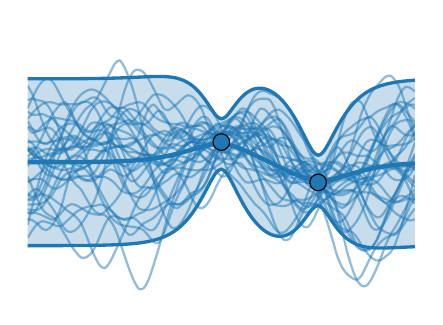
\begin{tikzpicture}
\begin{axis}[axis lines={none}, height={5cm}, width={6.5cm}, xmin={0}, xmax={1}, ymin={-1}, ymax={1}]
    \node at (0,-1) {};
    \node at (0,1) {};
    \node at (1,1) {};
    \node at (1,-1) {};
    \addplot[no markers, smooth, very thick, color={rgb,1:red,0.1216;green,0.4667;blue,0.7059}, name path={upper}]
        coordinates {
            (0.0,0.6199140961768654)
            (0.0125,0.6199425714927783)
            (0.025,0.6199783864581562)
            (0.0375,0.6200233662829112)
            (0.05,0.6200797656864601)
            (0.0625,0.6201503604553648)
            (0.075,0.6202385544841658)
            (0.0875,0.6203485030002299)
            (0.1,0.6204852515595847)
            (0.1125,0.6206548885126146)
            (0.125,0.6208647056109129)
            (0.1375,0.6211233567575545)
            (0.15,0.621440997918379)
            (0.1625,0.6218293810302168)
            (0.175,0.6223018602499781)
            (0.1875,0.6228732487414248)
            (0.2,0.6235594368715044)
            (0.2125,0.6243766466304895)
            (0.225,0.6253401510080454)
            (0.2375,0.6264622304388126)
            (0.25,0.6277490723629017)
            (0.2625,0.6291962483072014)
            (0.275,0.6307823339517931)
            (0.2875,0.6324601860223531)
            (0.3,0.6341453786837854)
            (0.3125,0.6357013651988239)
            (0.325,0.6369211143275115)
            (0.3375,0.6375053361068238)
            (0.35,0.6370380365657365)
            (0.3625,0.6349611286332626)
            (0.375,0.6305513230801723)
            (0.3875,0.6229047622218531)
            (0.4,0.6109382671624386)
            (0.4125,0.5934215336494578)
            (0.425,0.5690642064784973)
            (0.4375,0.5367009045678985)
            (0.45,0.49566153296827475)
            (0.4625,0.44653101260606376)
            (0.475,0.39282295507856513)
            (0.4875,0.34464685317516486)
            (0.5,0.3223754899538911)
            (0.5125,0.34058482839215576)
            (0.525,0.384306899691641)
            (0.5375,0.4328921481090502)
            (0.55,0.4759710490179375)
            (0.5625,0.5097228104055809)
            (0.575,0.5331850814547217)
            (0.5875,0.5465650120806383)
            (0.6,0.550466283604794)
            (0.6125,0.5455091311136459)
            (0.625,0.5321433216808108)
            (0.6375,0.5105731241442092)
            (0.65,0.48076057857831844)
            (0.6625,0.44249708250720937)
            (0.675,0.39555086340542395)
            (0.6875,0.3399197388696741)
            (0.7,0.27626172251086917)
            (0.7125,0.2066879756831459)
            (0.725,0.1364141076992448)
            (0.7375,0.07731047248583253)
            (0.75,0.05131933524894594)
            (0.7625,0.07391456195380275)
            (0.775,0.1297864344643398)
            (0.7875,0.19704165770173115)
            (0.8,0.2638428314974382)
            (0.8125,0.3250571025562066)
            (0.825,0.37873286688001917)
            (0.8375,0.4244703945004936)
            (0.85,0.4626524185492334)
            (0.8625,0.4940380860362959)
            (0.875,0.5195326231804909)
            (0.8875,0.5400545925834024)
            (0.9,0.5564623693375389)
            (0.9125,0.5695178886612947)
            (0.925,0.5798737501423057)
            (0.9375,0.5880743919367857)
            (0.95,0.5945650652582235)
            (0.9625,0.5997044498028763)
            (0.975,0.6037782650292838)
            (0.9875,0.6070123114982292)
            (1.0,0.609584123231418)
        }
        ;
    \addplot[no markers, smooth, very thick, color={rgb,1:red,0.1216;green,0.4667;blue,0.7059}, name path={lower}]
        coordinates {
            (0.0,-0.6196984280758382)
            (0.0125,-0.6196697615027457)
            (0.025,-0.6196336420765757)
            (0.0375,-0.6195881786813756)
            (0.05,-0.6195310130566563)
            (0.0625,-0.6194592072375776)
            (0.075,-0.6193691041152474)
            (0.0875,-0.6192561544448133)
            (0.1,-0.619114701753299)
            (0.1125,-0.6189377140916881)
            (0.125,-0.6187164481996643)
            (0.1375,-0.6184400270871517)
            (0.15,-0.6180949058637912)
            (0.1625,-0.6176641923303977)
            (0.175,-0.6171267777354612)
            (0.1875,-0.6164562184610327)
            (0.2,-0.6156192905043797)
            (0.2125,-0.6145741149161671)
            (0.225,-0.6132677238051523)
            (0.2375,-0.6116329041373474)
            (0.25,-0.609584123231418)
            (0.2625,-0.6070123114982292)
            (0.275,-0.6037782650292838)
            (0.2875,-0.5997044498028763)
            (0.3,-0.5945650652582235)
            (0.3125,-0.5880743919367857)
            (0.325,-0.5798737501423057)
            (0.3375,-0.5695178886612947)
            (0.35,-0.5564623693375389)
            (0.3625,-0.5400545925834024)
            (0.375,-0.5195326231804909)
            (0.3875,-0.4940380860362959)
            (0.4,-0.4626524185492334)
            (0.4125,-0.4244703945004936)
            (0.425,-0.37873286688001917)
            (0.4375,-0.3250571025562066)
            (0.45,-0.26384283149743815)
            (0.4625,-0.1970416577017311)
            (0.475,-0.12978643446433968)
            (0.4875,-0.07391456195380261)
            (0.5,-0.05131933524894591)
            (0.5125,-0.07731047248583231)
            (0.525,-0.13641410769924478)
            (0.5375,-0.2066879756831459)
            (0.55,-0.2762617225108691)
            (0.5625,-0.33991973886967414)
            (0.575,-0.3955508634054239)
            (0.5875,-0.4424970825072093)
            (0.6,-0.4807605785783184)
            (0.6125,-0.5105731241442092)
            (0.625,-0.5321433216808108)
            (0.6375,-0.5455091311136459)
            (0.65,-0.550466283604794)
            (0.6625,-0.5465650120806383)
            (0.675,-0.5331850814547217)
            (0.6875,-0.5097228104055808)
            (0.7,-0.4759710490179376)
            (0.7125,-0.4328921481090502)
            (0.725,-0.384306899691641)
            (0.7375,-0.340584828392156)
            (0.75,-0.32237548995389104)
            (0.7625,-0.34464685317516497)
            (0.775,-0.39282295507856524)
            (0.7875,-0.4465310126060638)
            (0.8,-0.4956615329682747)
            (0.8125,-0.5367009045678985)
            (0.825,-0.5690642064784973)
            (0.8375,-0.5934215336494578)
            (0.85,-0.6109382671624386)
            (0.8625,-0.6229047622218531)
            (0.875,-0.6305513230801723)
            (0.8875,-0.6349611286332626)
            (0.9,-0.6370380365657365)
            (0.9125,-0.6375053361068238)
            (0.925,-0.6369211143275115)
            (0.9375,-0.6357013651988239)
            (0.95,-0.6341453786837854)
            (0.9625,-0.6324601860223531)
            (0.975,-0.6307823339517931)
            (0.9875,-0.6291962483072014)
            (1.0,-0.6277490723629017)
        }
        ;
    \addplot[color={rgb,1:red,0.1216;green,0.4667;blue,0.7059}, opacity={0.25}]
        fill between [of = upper and lower]
        ;
    \addplot[no markers, smooth, ultra thick, color={rgb,1:red,0.1216;green,0.4667;blue,0.7059}]
        coordinates {
            (0.0,0.0001078340505135923)
            (0.0125,0.00013640499501634866)
            (0.025,0.00017237219079020152)
            (0.0375,0.0002175938007678534)
            (0.05,0.0002743763149019563)
            (0.0625,0.0003455766088936026)
            (0.075,0.00043472518445922124)
            (0.0875,0.0005461742777083397)
            (0.1,0.000685274903142837)
            (0.1125,0.000858587210463329)
            (0.125,0.001074128705624313)
            (0.1375,0.001341664835201373)
            (0.15,0.0016730460272938975)
            (0.1625,0.0020825943499095264)
            (0.175,0.0025875412572585045)
            (0.1875,0.0032085151401960847)
            (0.2,0.003970073183562359)
            (0.2125,0.00490126585716125)
            (0.225,0.006036213601446627)
            (0.2375,0.007414663150732556)
            (0.25,0.009082474565741901)
            (0.2625,0.011091968404486107)
            (0.275,0.013502034461254683)
            (0.2875,0.016377868109738417)
            (0.3,0.019790156712780962)
            (0.3125,0.023813486631019086)
            (0.325,0.02852368209260293)
            (0.3375,0.03399372372276454)
            (0.35,0.04028783361409879)
            (0.3625,0.04745326802493011)
            (0.375,0.055509349949840706)
            (0.3875,0.06443333809277857)
            (0.4,0.07414292430660259)
            (0.4125,0.0844755695744821)
            (0.425,0.0951656697992391)
            (0.4375,0.10582190100584594)
            (0.45,0.11590935073541828)
            (0.4625,0.12474467745216633)
            (0.475,0.13151826030711272)
            (0.4875,0.1353661456106811)
            (0.5,0.13552807735247258)
            (0.5125,0.13163717795316174)
            (0.525,0.1239463959961981)
            (0.5375,0.11310208621295215)
            (0.55,0.09985466325353423)
            (0.5625,0.08490153576795335)
            (0.575,0.06881710902464885)
            (0.5875,0.052033964786714494)
            (0.6,0.034852852513237824)
            (0.6125,0.017468003484718372)
            (0.625,1.3877787807814457e-17)
            (0.6375,-0.017468003484718365)
            (0.65,-0.0348528525132378)
            (0.6625,-0.05203396478671447)
            (0.675,-0.06881710902464883)
            (0.6875,-0.08490153576795334)
            (0.7,-0.09985466325353419)
            (0.7125,-0.11310208621295215)
            (0.725,-0.12394639599619808)
            (0.7375,-0.13163717795316174)
            (0.75,-0.13552807735247255)
            (0.7625,-0.1353661456106811)
            (0.775,-0.13151826030711272)
            (0.7875,-0.12474467745216633)
            (0.8,-0.11590935073541825)
            (0.8125,-0.10582190100584593)
            (0.825,-0.09516566979923907)
            (0.8375,-0.08447556957448209)
            (0.85,-0.07414292430660258)
            (0.8625,-0.06443333809277857)
            (0.875,-0.05550934994984069)
            (0.8875,-0.047453268024930106)
            (0.9,-0.04028783361409878)
            (0.9125,-0.03399372372276453)
            (0.925,-0.028523682092602927)
            (0.9375,-0.023813486631019083)
            (0.95,-0.01979015671278096)
            (0.9625,-0.016377868109738413)
            (0.975,-0.013502034461254682)
            (0.9875,-0.011091968404486105)
            (1.0,-0.0090824745657419)
        }
        ;
    \addplot[no markers, smooth, thick, color={rgb,1:red,0.1216;green,0.4667;blue,0.7059}, opacity={0.5}]
        coordinates {
            (0.0,0.46327616462531745)
            (0.0125,0.47056472534562865)
            (0.025,0.4610649118046657)
            (0.0375,0.45393695922083455)
            (0.05,0.4278462902121283)
            (0.0625,0.3695379627135198)
            (0.075,0.28705006271148126)
            (0.0875,0.18472009223785932)
            (0.1,0.0789933829510629)
            (0.1125,-0.008622567736805642)
            (0.125,-0.05349691797469472)
            (0.1375,-0.05429968993699299)
            (0.15,-0.03458400839738065)
            (0.1625,-0.008669631549652834)
            (0.175,0.028723809657811183)
            (0.1875,0.07385527367187293)
            (0.2,0.10378814405004325)
            (0.2125,0.1101690064327496)
            (0.225,0.11209806416441528)
            (0.2375,0.11663342756848284)
            (0.25,0.11450712125342308)
            (0.2625,0.12182293704155164)
            (0.275,0.14290305290782696)
            (0.2875,0.21322875252625517)
            (0.3,0.31632153350348413)
            (0.3125,0.40043702867298575)
            (0.325,0.4279944108967263)
            (0.3375,0.3912050225579047)
            (0.35,0.33468226754687447)
            (0.3625,0.2927380467957139)
            (0.375,0.28571291661193177)
            (0.3875,0.2825624426208584)
            (0.4,0.27159122127969154)
            (0.4125,0.264099743450985)
            (0.425,0.252967517404504)
            (0.4375,0.2454507560549735)
            (0.45,0.23191859002107826)
            (0.4625,0.21988310757169194)
            (0.475,0.2150860264431309)
            (0.4875,0.19775381845380488)
            (0.5,0.17828721524240046)
            (0.5125,0.1483531765840125)
            (0.525,0.1357391291416097)
            (0.5375,0.16149417820129136)
            (0.55,0.182338688155979)
            (0.5625,0.19099492529191558)
            (0.575,0.1969663237226093)
            (0.5875,0.20669966379916704)
            (0.6,0.21833388590822278)
            (0.6125,0.23646305119878644)
            (0.625,0.26017799103313327)
            (0.6375,0.2661024107074954)
            (0.65,0.25305809165100873)
            (0.6625,0.22136845568762661)
            (0.675,0.1669286223393752)
            (0.6875,0.09997482119131927)
            (0.7,0.02989136761674757)
            (0.7125,-0.019731686688396408)
            (0.725,-0.05622836906948708)
            (0.7375,-0.07335887564046913)
            (0.75,-0.0923731327375684)
            (0.7625,-0.12593390077394867)
            (0.775,-0.152936188306109)
            (0.7875,-0.13985968007895944)
            (0.8,-0.10640989570638316)
            (0.8125,-0.08894553943439831)
            (0.825,-0.08635292912334845)
            (0.8375,-0.08689559706516187)
            (0.85,-0.07515204746282575)
            (0.8625,-0.05424363972800833)
            (0.875,-0.03623066236882627)
            (0.8875,-0.02841946533563651)
            (0.9,-0.019041640094853443)
            (0.9125,-0.03427368120968374)
            (0.925,-0.06854497753275729)
            (0.9375,-0.11179328182403028)
            (0.95,-0.13195440738360228)
            (0.9625,-0.13185920516747632)
            (0.975,-0.12037925361268124)
            (0.9875,-0.09092144367567298)
            (1.0,-0.034017002884056693)
        }
        ;
    \addplot[no markers, smooth, thick, color={rgb,1:red,0.1216;green,0.4667;blue,0.7059}, opacity={0.5}]
        coordinates {
            (0.0,-0.46415402839299114)
            (0.0125,-0.32117644850331417)
            (0.025,-0.18503188493740194)
            (0.0375,-0.05755128954727985)
            (0.05,0.05112297241892946)
            (0.0625,0.12828389286855557)
            (0.075,0.16998536078371113)
            (0.0875,0.1806049126173017)
            (0.1,0.18662269254342773)
            (0.1125,0.1970348012769312)
            (0.125,0.19228202273668948)
            (0.1375,0.1676424319239986)
            (0.15,0.14677799944099804)
            (0.1625,0.1352861782943414)
            (0.175,0.13805981414729557)
            (0.1875,0.13908082124209606)
            (0.2,0.15097098681310467)
            (0.2125,0.1439590965597404)
            (0.225,0.12813841638835935)
            (0.2375,0.11557536713608454)
            (0.25,0.1204586273199128)
            (0.2625,0.13741002637398803)
            (0.275,0.15054658879977845)
            (0.2875,0.16507000607853634)
            (0.3,0.1796770656129308)
            (0.3125,0.19730416499842174)
            (0.325,0.203214359148216)
            (0.3375,0.21646780175151867)
            (0.35,0.23227801497703746)
            (0.3625,0.22484127006432836)
            (0.375,0.1938750097729996)
            (0.3875,0.1750023457127488)
            (0.4,0.18437049112339432)
            (0.4125,0.21350929864071344)
            (0.425,0.2558909720554309)
            (0.4375,0.3040656465969561)
            (0.45,0.3366060312830993)
            (0.4625,0.331685485729166)
            (0.475,0.2802912062813832)
            (0.4875,0.1794721246161348)
            (0.5,0.06894996458196839)
            (0.5125,-0.03526501943503901)
            (0.525,-0.09854022420914241)
            (0.5375,-0.13073408280141968)
            (0.55,-0.1696998595166972)
            (0.5625,-0.2202122045980145)
            (0.575,-0.267043119789681)
            (0.5875,-0.3122822702049426)
            (0.6,-0.3448257977061495)
            (0.6125,-0.38561897768427733)
            (0.625,-0.4366063743482589)
            (0.6375,-0.491793699628644)
            (0.65,-0.523103021798894)
            (0.6625,-0.5193880638750024)
            (0.675,-0.487011986910051)
            (0.6875,-0.4381986298338928)
            (0.7,-0.38409833668258037)
            (0.7125,-0.3106538937159202)
            (0.725,-0.21519670780273045)
            (0.7375,-0.14071397257829227)
            (0.75,-0.08370429670499374)
            (0.7625,-0.02756577297241991)
            (0.775,0.03684666518948865)
            (0.7875,0.10814356589819224)
            (0.8,0.16323806516948303)
            (0.8125,0.18993197348752505)
            (0.825,0.20000816864900664)
            (0.8375,0.21125509646152457)
            (0.85,0.2361359506715384)
            (0.8625,0.28174474439387254)
            (0.875,0.3283018297290308)
            (0.8875,0.3316349179562845)
            (0.9,0.28975675125477507)
            (0.9125,0.2179327558822943)
            (0.925,0.134429269992572)
            (0.9375,0.057887402824865555)
            (0.95,-0.008590569899007743)
            (0.9625,-0.04981860662245094)
            (0.975,-0.06378739408813361)
            (0.9875,-0.058225312762714504)
            (1.0,-0.031406107478113)
        }
        ;
    \addplot[no markers, smooth, thick, color={rgb,1:red,0.1216;green,0.4667;blue,0.7059}, opacity={0.5}]
        coordinates {
            (0.0,0.25859064699223977)
            (0.0125,0.21869788598866324)
            (0.025,0.23206003003176748)
            (0.0375,0.27127996361172196)
            (0.05,0.30090890469249454)
            (0.0625,0.326217239695779)
            (0.075,0.3277135678833758)
            (0.0875,0.32316032744772866)
            (0.1,0.3146460297731594)
            (0.1125,0.3095526494473015)
            (0.125,0.29478493319496607)
            (0.1375,0.2740515785136973)
            (0.15,0.24084875348714205)
            (0.1625,0.23162123413581112)
            (0.175,0.25917638985968655)
            (0.1875,0.28574956067458296)
            (0.2,0.29259961816043467)
            (0.2125,0.2747838100312106)
            (0.225,0.25165469523398404)
            (0.2375,0.23872878201935968)
            (0.25,0.22537093607923378)
            (0.2625,0.20816315205805913)
            (0.275,0.17922671537916804)
            (0.2875,0.1359843802462654)
            (0.3,0.09070256722908623)
            (0.3125,0.05183625716304953)
            (0.325,0.01760079438659783)
            (0.3375,0.002269222409578102)
            (0.35,-0.010429407642595978)
            (0.3625,-0.0275282823964281)
            (0.375,-0.04299752312867928)
            (0.3875,-0.07885154347127829)
            (0.4,-0.12945973422271762)
            (0.4125,-0.19450148035159043)
            (0.425,-0.2743929090054619)
            (0.4375,-0.3264347201435822)
            (0.45,-0.3416059705581022)
            (0.4625,-0.313833647444656)
            (0.475,-0.2559029518459407)
            (0.4875,-0.1774341756440898)
            (0.5,-0.11099858289905896)
            (0.5125,-0.057294339765215446)
            (0.525,-0.02320703155070905)
            (0.5375,-0.006263966665182433)
            (0.55,-0.0068231416047543625)
            (0.5625,-0.046049604496429836)
            (0.575,-0.11386370772404303)
            (0.5875,-0.18998102907417524)
            (0.6,-0.2532789050468462)
            (0.6125,-0.2972190645306606)
            (0.625,-0.3163749197933382)
            (0.6375,-0.31201883631406074)
            (0.65,-0.29858326175807837)
            (0.6625,-0.2546714795051847)
            (0.675,-0.19204869816696676)
            (0.6875,-0.1346363961967974)
            (0.7,-0.09238965393754593)
            (0.7125,-0.07186436334560668)
            (0.725,-0.06583451793470578)
            (0.7375,-0.04410166336484814)
            (0.75,-0.016084824908278526)
            (0.7625,-0.006750596062794455)
            (0.775,0.0006797833547557142)
            (0.7875,-0.00043821721069042807)
            (0.8,-0.013803246716105479)
            (0.8125,-0.041291203650048076)
            (0.825,-0.07392278502734113)
            (0.8375,-0.09786417675329499)
            (0.85,-0.1503565614970383)
            (0.8625,-0.24130403667188915)
            (0.875,-0.32026184839744265)
            (0.8875,-0.37376300921749916)
            (0.9,-0.40777850554808187)
            (0.9125,-0.40122454518634776)
            (0.925,-0.351765081570814)
            (0.9375,-0.2849899360543703)
            (0.95,-0.22549785590848745)
            (0.9625,-0.1579184005279801)
            (0.975,-0.06553707076702234)
            (0.9875,0.042702444719172464)
            (1.0,0.14711885495544452)
        }
        ;
    \addplot[no markers, smooth, thick, color={rgb,1:red,0.1216;green,0.4667;blue,0.7059}, opacity={0.5}]
        coordinates {
            (0.0,-0.2297346933623143)
            (0.0125,-0.2572638385154083)
            (0.025,-0.22823726229541622)
            (0.0375,-0.14709512505761124)
            (0.05,-0.05010983401739522)
            (0.0625,0.03832731749399659)
            (0.075,0.0894349061305827)
            (0.0875,0.10257464930328661)
            (0.1,0.09673818807480167)
            (0.1125,0.0941167454883363)
            (0.125,0.11966739925997844)
            (0.1375,0.1790490853668309)
            (0.15,0.24102961843679455)
            (0.1625,0.2864881693716348)
            (0.175,0.29587326421214843)
            (0.1875,0.2895721426498672)
            (0.2,0.26564290237898386)
            (0.2125,0.200381298858337)
            (0.225,0.11578666488199614)
            (0.2375,0.02900665505302335)
            (0.25,-0.06012210365312565)
            (0.2625,-0.12986822652084215)
            (0.275,-0.14153989824142946)
            (0.2875,-0.10841169097679633)
            (0.3,-0.06365816297865479)
            (0.3125,-0.017996651277764314)
            (0.325,0.028424928494915)
            (0.3375,0.060554182152052966)
            (0.35,0.09609076292336265)
            (0.3625,0.12283633909648314)
            (0.375,0.1346303748478632)
            (0.3875,0.128104940657066)
            (0.4,0.11866539838090262)
            (0.4125,0.12965289527896545)
            (0.425,0.15757223709688914)
            (0.4375,0.16823368354125054)
            (0.45,0.16722530974703873)
            (0.4625,0.17267488882713175)
            (0.475,0.19469147919432822)
            (0.4875,0.22548735858983585)
            (0.5,0.26404449307744327)
            (0.5125,0.29008412991077026)
            (0.525,0.3226841301887742)
            (0.5375,0.3544139502293709)
            (0.55,0.37404545151340474)
            (0.5625,0.37785647190980626)
            (0.575,0.3654797100940335)
            (0.5875,0.3319645516242268)
            (0.6,0.2938561355285484)
            (0.6125,0.2578904671894455)
            (0.625,0.19180000514343792)
            (0.6375,0.08920502283529896)
            (0.65,-0.012510400206336467)
            (0.6625,-0.09229150164365622)
            (0.675,-0.1359497857676339)
            (0.6875,-0.1518632042971937)
            (0.7,-0.1498664800869096)
            (0.7125,-0.14632887588181695)
            (0.725,-0.15330894207996337)
            (0.7375,-0.150381918863337)
            (0.75,-0.12131284129958897)
            (0.7625,-0.07605743289570971)
            (0.775,-0.05000741990832468)
            (0.7875,-0.050185687645752236)
            (0.8,-0.07307527179214869)
            (0.8125,-0.09722729581766287)
            (0.825,-0.08866776860215159)
            (0.8375,-0.05080482794174354)
            (0.85,0.020932915556488595)
            (0.8625,0.09330393213281434)
            (0.875,0.14985814338933198)
            (0.8875,0.1682912694124485)
            (0.9,0.1597701806282153)
            (0.9125,0.14232387168506877)
            (0.925,0.10724577652941124)
            (0.9375,0.06244422619044509)
            (0.95,0.017959974202456375)
            (0.9625,-0.01334712388147976)
            (0.975,-0.02489095571533942)
            (0.9875,-0.03323985019265719)
            (1.0,-0.030222372913538496)
        }
        ;
    \addplot[no markers, smooth, thick, color={rgb,1:red,0.1216;green,0.4667;blue,0.7059}, opacity={0.5}]
        coordinates {
            (0.0,-0.10432377669974378)
            (0.0125,-0.1910469210093288)
            (0.025,-0.2750445128741369)
            (0.0375,-0.3456985693399386)
            (0.05,-0.38469778865807763)
            (0.0625,-0.4051535455807497)
            (0.075,-0.434152881615292)
            (0.0875,-0.49681856899757115)
            (0.1,-0.5566765063067888)
            (0.1125,-0.6208442269351554)
            (0.125,-0.6693950457177844)
            (0.1375,-0.7079313838584287)
            (0.15,-0.7070136209203337)
            (0.1625,-0.6815568985193495)
            (0.175,-0.6256242498621093)
            (0.1875,-0.5430735757466892)
            (0.2,-0.45733745836315237)
            (0.2125,-0.40691001065485044)
            (0.225,-0.40238154013651056)
            (0.2375,-0.41614479904488033)
            (0.25,-0.4282373929682477)
            (0.2625,-0.4220515965747485)
            (0.275,-0.39937433843558656)
            (0.2875,-0.3810775781588521)
            (0.3,-0.36645055842958196)
            (0.3125,-0.3261871236505049)
            (0.325,-0.25583811770625864)
            (0.3375,-0.17458347282920733)
            (0.35,-0.09714102534512295)
            (0.3625,-0.03225210082657574)
            (0.375,0.0258145020018139)
            (0.3875,0.07738196938780321)
            (0.4,0.11192035057811789)
            (0.4125,0.1390420510775431)
            (0.425,0.15205624719357833)
            (0.4375,0.1441466356829393)
            (0.45,0.12444335234865453)
            (0.4625,0.12073123753026446)
            (0.475,0.1339245822508692)
            (0.4875,0.16695830583970206)
            (0.5,0.20889832027404454)
            (0.5125,0.2660515875261863)
            (0.525,0.3205602773381063)
            (0.5375,0.33755898693847297)
            (0.55,0.3263200827134582)
            (0.5625,0.29698527356429405)
            (0.575,0.24406956235871202)
            (0.5875,0.17348608443138164)
            (0.6,0.0981817524494086)
            (0.6125,0.028796840694921416)
            (0.625,-0.03977472725200765)
            (0.6375,-0.08433586488335656)
            (0.65,-0.09290997868876043)
            (0.6625,-0.07673875790518729)
            (0.675,-0.059107854439077075)
            (0.6875,-0.046723168044038005)
            (0.7,-0.06843412179610067)
            (0.7125,-0.11700438364127524)
            (0.725,-0.1549376258177356)
            (0.7375,-0.15412352435873392)
            (0.75,-0.11626601212830961)
            (0.7625,-0.046619938132366846)
            (0.775,0.02617160584465345)
            (0.7875,0.08270600146950946)
            (0.8,0.1122645278788338)
            (0.8125,0.07942439048411845)
            (0.825,8.95218763675848e-5)
            (0.8375,-0.0779681015138787)
            (0.85,-0.15558979068019896)
            (0.8625,-0.24659874578491034)
            (0.875,-0.33090985076887225)
            (0.8875,-0.3979173158826736)
            (0.9,-0.4636049886666618)
            (0.9125,-0.4994022006968328)
            (0.925,-0.5208056446166703)
            (0.9375,-0.5327106631967231)
            (0.95,-0.5269934593650284)
            (0.9625,-0.4803813331096039)
            (0.975,-0.4070157281377132)
            (0.9875,-0.32150908731190275)
            (1.0,-0.2662836421416675)
        }
        ;
    \addplot[no markers, smooth, thick, color={rgb,1:red,0.1216;green,0.4667;blue,0.7059}, opacity={0.5}]
        coordinates {
            (0.0,-0.13963639358265764)
            (0.0125,-0.12608177445935698)
            (0.025,-0.12383994841538547)
            (0.0375,-0.1278198928358803)
            (0.05,-0.15842405993494374)
            (0.0625,-0.19019854516707727)
            (0.075,-0.19575122701083406)
            (0.0875,-0.1760632336053225)
            (0.1,-0.14721312064268008)
            (0.1125,-0.10449259292528446)
            (0.125,-0.0687833177273133)
            (0.1375,-0.028819402230610615)
            (0.15,0.03732666365690964)
            (0.1625,0.1107533183734305)
            (0.175,0.17342411862238652)
            (0.1875,0.20721696395047234)
            (0.2,0.21698619358907578)
            (0.2125,0.21447269069497052)
            (0.225,0.18480227971429117)
            (0.2375,0.1286801872019202)
            (0.25,0.04377110379046294)
            (0.2625,-0.049826685461038175)
            (0.275,-0.13372502987538354)
            (0.2875,-0.17890637338524273)
            (0.3,-0.1864580018158932)
            (0.3125,-0.1861797200183189)
            (0.325,-0.18828978309850675)
            (0.3375,-0.16018702284309644)
            (0.35,-0.11158379186575962)
            (0.3625,-0.052141394815210906)
            (0.375,-0.0006928760624740071)
            (0.3875,0.03604590994422352)
            (0.4,0.08951313492402593)
            (0.4125,0.13757864747015924)
            (0.425,0.15206226582974194)
            (0.4375,0.14526301973667982)
            (0.45,0.14389966025870332)
            (0.4625,0.1471515914525368)
            (0.475,0.14532288149957617)
            (0.4875,0.15442292173176642)
            (0.5,0.16657073813900902)
            (0.5125,0.18468796540657795)
            (0.525,0.21641880994604756)
            (0.5375,0.2478675472074463)
            (0.55,0.26765868183126484)
            (0.5625,0.2686067473168906)
            (0.575,0.2604419241061229)
            (0.5875,0.2567473325935197)
            (0.6,0.2743686455411833)
            (0.6125,0.31675026423564967)
            (0.625,0.3589995634544646)
            (0.6375,0.3855781354824517)
            (0.65,0.39021240076774844)
            (0.6625,0.36363726545798236)
            (0.675,0.32665632524480737)
            (0.6875,0.2777567744844496)
            (0.7,0.22039572426725343)
            (0.7125,0.17131028279810298)
            (0.725,0.11708907884139427)
            (0.7375,0.03745961749432031)
            (0.75,-0.0620239646458675)
            (0.7625,-0.17038069295627115)
            (0.775,-0.2890291689516967)
            (0.7875,-0.40208884168392195)
            (0.8,-0.46556664639121137)
            (0.8125,-0.49268640060146746)
            (0.825,-0.5056937975333224)
            (0.8375,-0.5184901821773317)
            (0.85,-0.5568916918779095)
            (0.8625,-0.6198343489268157)
            (0.875,-0.6698639209308973)
            (0.8875,-0.7080754471462823)
            (0.9,-0.7290704568728676)
            (0.9125,-0.7254384114320289)
            (0.925,-0.6978745016558879)
            (0.9375,-0.6672665989497416)
            (0.95,-0.5987084533352424)
            (0.9625,-0.493980968021341)
            (0.975,-0.3718578502540846)
            (0.9875,-0.2376249415243876)
            (1.0,-0.09411257068121326)
        }
        ;
    \addplot[no markers, smooth, thick, color={rgb,1:red,0.1216;green,0.4667;blue,0.7059}, opacity={0.5}]
        coordinates {
            (0.0,0.14585090985836768)
            (0.0125,0.15384109823932557)
            (0.025,0.15377073349915168)
            (0.0375,0.1436214618419241)
            (0.05,0.1427073426340983)
            (0.0625,0.15511017156599047)
            (0.075,0.15795960462333006)
            (0.0875,0.16866127790019786)
            (0.1,0.17443437680349197)
            (0.1125,0.16203153267257545)
            (0.125,0.12966345346125308)
            (0.1375,0.10324260159203569)
            (0.15,0.09753958978146611)
            (0.1625,0.14372729368325599)
            (0.175,0.21953171629805265)
            (0.1875,0.274567791736774)
            (0.2,0.30051906752593804)
            (0.2125,0.3187776481866942)
            (0.225,0.36029624830095885)
            (0.2375,0.40062428375788955)
            (0.25,0.40282245340642564)
            (0.2625,0.36684977606958846)
            (0.275,0.3210937132991707)
            (0.2875,0.2855500003053438)
            (0.3,0.2810567558006008)
            (0.3125,0.3002145808395383)
            (0.325,0.34691663710236303)
            (0.3375,0.3832565715388629)
            (0.35,0.36160562423737375)
            (0.3625,0.2986902760063787)
            (0.375,0.22961233958435323)
            (0.3875,0.1889817890353378)
            (0.4,0.2101202000877373)
            (0.4125,0.27815214738872196)
            (0.425,0.34734731863542057)
            (0.4375,0.3956289509228111)
            (0.45,0.4205655924206687)
            (0.4625,0.41088799498524053)
            (0.475,0.3803567782938554)
            (0.4875,0.32741917546859123)
            (0.5,0.24758299393642585)
            (0.5125,0.14127637082759176)
            (0.525,0.03559872022326904)
            (0.5375,-0.04605274979649554)
            (0.55,-0.10627488115626882)
            (0.5625,-0.14690576512074327)
            (0.575,-0.15059576272390163)
            (0.5875,-0.1410530496644617)
            (0.6,-0.12908569242106654)
            (0.6125,-0.1261006936610428)
            (0.625,-0.14100056957076745)
            (0.6375,-0.15343294933430615)
            (0.65,-0.15460440407895737)
            (0.6625,-0.13037684507924505)
            (0.675,-0.08262454377120976)
            (0.6875,-0.04490915352283492)
            (0.7,-0.018861355166039064)
            (0.7125,-0.0020502748365516937)
            (0.725,0.0073424393490444245)
            (0.7375,0.0029954269081960416)
            (0.75,-0.0069696112777867525)
            (0.7625,-0.019659483787510146)
            (0.775,-0.019155670455722376)
            (0.7875,-0.0376647051907449)
            (0.8,-0.06423561570500813)
            (0.8125,-0.10152462123705314)
            (0.825,-0.11973335909135241)
            (0.8375,-0.1184985396626722)
            (0.85,-0.10214085723502313)
            (0.8625,-0.06885291396277403)
            (0.875,-0.007600348915869283)
            (0.8875,0.08685706052798009)
            (0.9,0.18679529436838707)
            (0.9125,0.2738972087581689)
            (0.925,0.35192851229272804)
            (0.9375,0.414064172063288)
            (0.95,0.4352082048761239)
            (0.9625,0.4049993292152464)
            (0.975,0.3451502654857796)
            (0.9875,0.26885495660907593)
            (1.0,0.16738566926039333)
        }
        ;
    \addplot[no markers, smooth, thick, color={rgb,1:red,0.1216;green,0.4667;blue,0.7059}, opacity={0.5}]
        coordinates {
            (0.0,0.3215827163171843)
            (0.0125,0.36607751419648527)
            (0.025,0.4031124168196027)
            (0.0375,0.43158900517528587)
            (0.05,0.4455250465542042)
            (0.0625,0.4448549743601418)
            (0.075,0.4344636657315714)
            (0.0875,0.42807420902344673)
            (0.1,0.4299045233057847)
            (0.1125,0.4318462721417049)
            (0.125,0.4310239687568033)
            (0.1375,0.4376872232445169)
            (0.15,0.4553573573276545)
            (0.1625,0.4761259840467089)
            (0.175,0.48182786745895456)
            (0.1875,0.45412089768422836)
            (0.2,0.3931963208517177)
            (0.2125,0.34792436391267645)
            (0.225,0.33541322133428075)
            (0.2375,0.3229105997876348)
            (0.25,0.30084680280142867)
            (0.2625,0.2896023454462915)
            (0.275,0.3140899983739296)
            (0.2875,0.36042489066714595)
            (0.3,0.4107991345772878)
            (0.3125,0.4625788313026381)
            (0.325,0.5007367325391124)
            (0.3375,0.504090649405937)
            (0.35,0.4948615398283527)
            (0.3625,0.4697203228324972)
            (0.375,0.43457044997332944)
            (0.3875,0.392951545383902)
            (0.4,0.3390148825254098)
            (0.4125,0.2719538882838395)
            (0.425,0.19945428710653684)
            (0.4375,0.1320283674542136)
            (0.45,0.10116670721417662)
            (0.4625,0.08392991466736294)
            (0.475,0.05500894874546534)
            (0.4875,0.029740882184996605)
            (0.5,0.014910182792038283)
            (0.5125,-0.009041623946541184)
            (0.525,-0.013927581696214282)
            (0.5375,0.0077411224940890245)
            (0.55,0.06705425564069414)
            (0.5625,0.1522490133897204)
            (0.575,0.24678710046018731)
            (0.5875,0.3407625399892539)
            (0.6,0.3963698452045248)
            (0.6125,0.3906332572223866)
            (0.625,0.3514947150665284)
            (0.6375,0.3083876356722151)
            (0.65,0.2625808431688419)
            (0.6625,0.21567722275380202)
            (0.675,0.16563825849253677)
            (0.6875,0.10892019167199879)
            (0.7,0.04446784327890141)
            (0.7125,-0.024167558725022742)
            (0.725,-0.08898321617838861)
            (0.7375,-0.13957728427307942)
            (0.75,-0.1826860145386976)
            (0.7625,-0.21007557305519953)
            (0.775,-0.22025477842237295)
            (0.7875,-0.23118401598116534)
            (0.8,-0.24431483371914817)
            (0.8125,-0.24392285671446717)
            (0.825,-0.23152126021569003)
            (0.8375,-0.21230468230794067)
            (0.85,-0.18906482934341867)
            (0.8625,-0.1596095938076854)
            (0.875,-0.12268427101568541)
            (0.8875,-0.057116308028670015)
            (0.9,0.04789383042630771)
            (0.9125,0.14447794693961996)
            (0.925,0.21232501339105847)
            (0.9375,0.2574797256680895)
            (0.95,0.3060140516110821)
            (0.9625,0.36764553673152844)
            (0.975,0.4233719842044159)
            (0.9875,0.45166767877294167)
            (1.0,0.4775545785353789)
        }
        ;
    \addplot[no markers, smooth, thick, color={rgb,1:red,0.1216;green,0.4667;blue,0.7059}, opacity={0.5}]
        coordinates {
            (0.0,-0.03024923774134428)
            (0.0125,0.02245179415370345)
            (0.025,0.0676937767025771)
            (0.0375,0.0880988916158829)
            (0.05,0.09853504149558551)
            (0.0625,0.09617129644003983)
            (0.075,0.08922185843492189)
            (0.0875,0.08566028743399137)
            (0.1,0.09196478669986104)
            (0.1125,0.10880933817729868)
            (0.125,0.12680026050913584)
            (0.1375,0.14071710358855513)
            (0.15,0.164100701128047)
            (0.1625,0.1763473725505299)
            (0.175,0.16349934035442823)
            (0.1875,0.14088981140393364)
            (0.2,0.09933679140828966)
            (0.2125,0.041306333511317496)
            (0.225,-0.03211622447323409)
            (0.2375,-0.11080114631320663)
            (0.25,-0.18747210818970048)
            (0.2625,-0.22915002830978312)
            (0.275,-0.25038016000084024)
            (0.2875,-0.2628437618209962)
            (0.3,-0.2524558105282134)
            (0.3125,-0.22020073539323898)
            (0.325,-0.1597786295787062)
            (0.3375,-0.10559704105013645)
            (0.35,-0.06436824063383978)
            (0.3625,-0.04966568722881862)
            (0.375,-0.04928020537653244)
            (0.3875,-0.040799209872863146)
            (0.4,-0.04324003560641379)
            (0.4125,-0.0521286581811915)
            (0.425,-0.05695198181183142)
            (0.4375,-0.06059019762179252)
            (0.45,-0.05042627512382725)
            (0.4625,-0.018981834035511902)
            (0.475,0.034353735795283724)
            (0.4875,0.0737350311062332)
            (0.5,0.09808756285965586)
            (0.5125,0.11409767544195554)
            (0.525,0.11952304529780425)
            (0.5375,0.12475359341238354)
            (0.55,0.13649834583787399)
            (0.5625,0.15488525971401645)
            (0.575,0.18592485953828275)
            (0.5875,0.21688297585895389)
            (0.6,0.26198300018267634)
            (0.6125,0.3067227765677762)
            (0.625,0.3317429775141112)
            (0.6375,0.3394161078452228)
            (0.65,0.32162803297122905)
            (0.6625,0.2764268451231419)
            (0.675,0.21358254479205746)
            (0.6875,0.12691881564196625)
            (0.7,0.022711404243204558)
            (0.7125,-0.07582869053882366)
            (0.725,-0.13412993698995102)
            (0.7375,-0.16950567106555056)
            (0.75,-0.20658297745960688)
            (0.7625,-0.2840785253524979)
            (0.775,-0.3653466575307325)
            (0.7875,-0.41946209424150827)
            (0.8,-0.44667744743193283)
            (0.8125,-0.4340712504612555)
            (0.825,-0.3915583657107645)
            (0.8375,-0.32535095969123357)
            (0.85,-0.25041988856148456)
            (0.8625,-0.17579084090055508)
            (0.875,-0.1056913414653713)
            (0.8875,-0.04461794265091999)
            (0.9,0.009434834299098221)
            (0.9125,0.05832855524827483)
            (0.925,0.0940350291975431)
            (0.9375,0.10459641419257966)
            (0.95,0.12384642462420517)
            (0.9625,0.1569040332159491)
            (0.975,0.19971561761291284)
            (0.9875,0.23989839642584715)
            (1.0,0.2764040002019933)
        }
        ;
    \addplot[no markers, smooth, thick, color={rgb,1:red,0.1216;green,0.4667;blue,0.7059}, opacity={0.5}]
        coordinates {
            (0.0,0.3065537247195646)
            (0.0125,0.2449462348697751)
            (0.025,0.17838676528436845)
            (0.0375,0.14323695821055857)
            (0.05,0.13480621785756566)
            (0.0625,0.1669430603106301)
            (0.075,0.22207384183779852)
            (0.0875,0.26184682642801105)
            (0.1,0.2802155718034161)
            (0.1125,0.2881165611945197)
            (0.125,0.2806545515390234)
            (0.1375,0.2531728224942236)
            (0.15,0.22666524099461852)
            (0.1625,0.22252067493818786)
            (0.175,0.23337054808553556)
            (0.1875,0.2400950451382976)
            (0.2,0.21947097736816137)
            (0.2125,0.16753578729738827)
            (0.225,0.12634415300181395)
            (0.2375,0.1107578285108317)
            (0.25,0.08963413260476578)
            (0.2625,0.07401167022479488)
            (0.275,0.07627060663956099)
            (0.2875,0.06396357888371527)
            (0.3,0.05464393932215994)
            (0.3125,0.059028577076182594)
            (0.325,0.05312033432471251)
            (0.3375,0.035655332285002485)
            (0.35,-0.0021608068251629635)
            (0.3625,-0.026116254462671937)
            (0.375,-0.012831869039942972)
            (0.3875,0.03818460115046164)
            (0.4,0.09404682375968318)
            (0.4125,0.15201184719322672)
            (0.425,0.22026284233794677)
            (0.4375,0.2807123993360897)
            (0.45,0.30023533804237285)
            (0.4625,0.28388772749553737)
            (0.475,0.24869606498879218)
            (0.4875,0.21212254115215934)
            (0.5,0.1857282549250793)
            (0.5125,0.16028748379680757)
            (0.525,0.12619459678405415)
            (0.5375,0.10223533434376539)
            (0.55,0.07500096767524336)
            (0.5625,0.033767672586959147)
            (0.575,-0.019983348284789197)
            (0.5875,-0.05377311551293515)
            (0.6,-0.0673361799030461)
            (0.6125,-0.08794843379182227)
            (0.625,-0.09686668023543527)
            (0.6375,-0.08958635336480651)
            (0.65,-0.05920520422988386)
            (0.6625,-0.028229235759410484)
            (0.675,0.004814077137072381)
            (0.6875,0.018934211899539727)
            (0.7,0.010667812196095194)
            (0.7125,-0.0016017591064544645)
            (0.725,-0.05307570432423314)
            (0.7375,-0.14345317514651135)
            (0.75,-0.25061911664057995)
            (0.7625,-0.35415289988960963)
            (0.775,-0.458408446491133)
            (0.7875,-0.5799752413525501)
            (0.8,-0.7017254097362784)
            (0.8125,-0.7838212618722047)
            (0.825,-0.8302546632358897)
            (0.8375,-0.8590219895054334)
            (0.85,-0.8734322444604917)
            (0.8625,-0.8398777066577229)
            (0.875,-0.7671775786391001)
            (0.8875,-0.6932793039649306)
            (0.9,-0.6313631762203203)
            (0.9125,-0.5886205901629448)
            (0.925,-0.5616136347811165)
            (0.9375,-0.5453064191938569)
            (0.95,-0.5364616469185212)
            (0.9625,-0.5000147816394603)
            (0.975,-0.44783784044682456)
            (0.9875,-0.39029591234181)
            (1.0,-0.3444029570559046)
        }
        ;
    \addplot[no markers, smooth, thick, color={rgb,1:red,0.1216;green,0.4667;blue,0.7059}, opacity={0.5}]
        coordinates {
            (0.0,0.4006461238645812)
            (0.0125,0.48078751022483424)
            (0.025,0.5511789921964699)
            (0.0375,0.6000850054862888)
            (0.05,0.620772349283791)
            (0.0625,0.6049117534569555)
            (0.075,0.5507091004377603)
            (0.0875,0.4787563226761112)
            (0.1,0.4157624367835003)
            (0.1125,0.3525467278648776)
            (0.125,0.2894197873450285)
            (0.1375,0.23544649425575345)
            (0.15,0.20177685226002415)
            (0.1625,0.17945016202148484)
            (0.175,0.1650601506287221)
            (0.1875,0.17878662431074765)
            (0.2,0.2275038159383728)
            (0.2125,0.26763482349016277)
            (0.225,0.28317392616914067)
            (0.2375,0.2900308288012061)
            (0.25,0.30460095140567744)
            (0.2625,0.31352506467020946)
            (0.275,0.29730063379577587)
            (0.2875,0.2580240511324496)
            (0.3,0.21909198451492276)
            (0.3125,0.17966098172971262)
            (0.325,0.13896767758323378)
            (0.3375,0.1024247632000031)
            (0.35,0.060117330869836894)
            (0.3625,0.03794010219191685)
            (0.375,0.043834309411534766)
            (0.3875,0.04476482069760007)
            (0.4,0.04274064910689812)
            (0.4125,0.030642182644779137)
            (0.425,0.015775395414370008)
            (0.4375,0.0035731899284980884)
            (0.45,0.005866297003973231)
            (0.4625,0.030209007381569508)
            (0.475,0.07392199027349)
            (0.4875,0.10243561913688704)
            (0.5,0.0998650365929975)
            (0.5125,0.07912625986148891)
            (0.525,0.058786414247201435)
            (0.5375,0.042907873688674214)
            (0.55,0.03677234705377119)
            (0.5625,0.0512968057858908)
            (0.575,0.07560045157039097)
            (0.5875,0.10522669676446672)
            (0.6,0.12002807811010213)
            (0.6125,0.13520927270797362)
            (0.625,0.16601058408087738)
            (0.6375,0.17055994357128906)
            (0.65,0.14770430335585438)
            (0.6625,0.09618426052894441)
            (0.675,0.028967897410336396)
            (0.6875,-0.02389494950155885)
            (0.7,-0.04430649596831915)
            (0.7125,-0.057065069979951866)
            (0.725,-0.06491926296887018)
            (0.7375,-0.0854976049488812)
            (0.75,-0.12813198219587107)
            (0.7625,-0.17747331649805742)
            (0.775,-0.2292529710293727)
            (0.7875,-0.2870207443477837)
            (0.8,-0.35152340271041493)
            (0.8125,-0.4321193420817995)
            (0.825,-0.5100197799295731)
            (0.8375,-0.5747823243137925)
            (0.85,-0.6289730305761002)
            (0.8625,-0.6530587841382935)
            (0.875,-0.6565154485552537)
            (0.8875,-0.6394901661006477)
            (0.9,-0.5818416006480911)
            (0.9125,-0.4919704319012818)
            (0.925,-0.3965905314194756)
            (0.9375,-0.31593195128584456)
            (0.95,-0.26926882538293334)
            (0.9625,-0.2502338966626213)
            (0.975,-0.25711860274668147)
            (0.9875,-0.27541169914306834)
            (1.0,-0.3053415209795728)
        }
        ;
    \addplot[no markers, smooth, thick, color={rgb,1:red,0.1216;green,0.4667;blue,0.7059}, opacity={0.5}]
        coordinates {
            (0.0,0.11603927278445117)
            (0.0125,0.0763104301400412)
            (0.025,0.037094368370236025)
            (0.0375,0.017364238183551657)
            (0.05,0.014357121847561242)
            (0.0625,0.015412552676906296)
            (0.075,0.010917000205492272)
            (0.0875,-0.005121978706788378)
            (0.1,-0.0522481824899908)
            (0.1125,-0.12207511830248909)
            (0.125,-0.16727877480973258)
            (0.1375,-0.2012129173477493)
            (0.15,-0.2625191415303647)
            (0.1625,-0.32318848416698426)
            (0.175,-0.36871642639306323)
            (0.1875,-0.3847103204632351)
            (0.2,-0.39501124825277006)
            (0.2125,-0.43031675778424733)
            (0.225,-0.49015141808722357)
            (0.2375,-0.5853110778888567)
            (0.25,-0.6943737630122274)
            (0.2625,-0.7973597417961151)
            (0.275,-0.8844483151296094)
            (0.2875,-0.9410979664631136)
            (0.3,-0.9344645282053413)
            (0.3125,-0.8700654827080424)
            (0.325,-0.7649688981213577)
            (0.3375,-0.6468592966113964)
            (0.35,-0.5195678228937032)
            (0.3625,-0.3924832789699944)
            (0.375,-0.2806675202936598)
            (0.3875,-0.1764030704041749)
            (0.4,-0.07278650309920495)
            (0.4125,0.014238560372354922)
            (0.425,0.06089434281518128)
            (0.4375,0.06343931230491748)
            (0.45,0.047128336256526494)
            (0.4625,0.015655818485585074)
            (0.475,-0.020680924119217244)
            (0.4875,-0.06646491422938354)
            (0.5,-0.10379345435231652)
            (0.5125,-0.10092198688719546)
            (0.525,-0.054063306310828514)
            (0.5375,0.022087426667723377)
            (0.55,0.08643527251193396)
            (0.5625,0.1341275684626541)
            (0.575,0.17784168480885162)
            (0.5875,0.20610907514769716)
            (0.6,0.23142189212286468)
            (0.6125,0.25826968798594796)
            (0.625,0.2856746470326877)
            (0.6375,0.3133870317574731)
            (0.65,0.31733795827047206)
            (0.6625,0.26124825644631916)
            (0.675,0.1761882121577118)
            (0.6875,0.09452785737717098)
            (0.7,0.025431498470129262)
            (0.7125,-0.03915455592277172)
            (0.725,-0.10833443985316007)
            (0.7375,-0.17900242977470304)
            (0.75,-0.21798510623906736)
            (0.7625,-0.22542039852960594)
            (0.775,-0.20757236814347496)
            (0.7875,-0.17008487809427822)
            (0.8,-0.13644066074605518)
            (0.8125,-0.11121917396663004)
            (0.825,-0.100272357600056)
            (0.8375,-0.10694946863534154)
            (0.85,-0.12108246671759963)
            (0.8625,-0.1223711028452138)
            (0.875,-0.11500941910415326)
            (0.8875,-0.106638409347313)
            (0.9,-0.10043107740263672)
            (0.9125,-0.0908123797533646)
            (0.925,-0.07287917627416994)
            (0.9375,-0.05366526250379419)
            (0.95,-0.04407312759617997)
            (0.9625,-0.04136145284075046)
            (0.975,-0.02720577305428836)
            (0.9875,-0.024357683552536265)
            (1.0,-0.059419649059748794)
        }
        ;
    \addplot[no markers, smooth, thick, color={rgb,1:red,0.1216;green,0.4667;blue,0.7059}, opacity={0.5}]
        coordinates {
            (0.0,0.08637606637339759)
            (0.0125,0.10628055574784867)
            (0.025,0.10944692885677741)
            (0.0375,0.08588298625577782)
            (0.05,0.05885813954247077)
            (0.0625,0.04711886567670239)
            (0.075,0.06832106295315243)
            (0.0875,0.10520446675675543)
            (0.1,0.14798458905525677)
            (0.1125,0.1795448342618199)
            (0.125,0.1779046382156575)
            (0.1375,0.13104265281108093)
            (0.15,0.04942993801377486)
            (0.1625,-0.06462084570697102)
            (0.175,-0.16934060596757153)
            (0.1875,-0.2575495272751472)
            (0.2,-0.33286080641344357)
            (0.2125,-0.400356638448704)
            (0.225,-0.4361679377466462)
            (0.2375,-0.4622991537538107)
            (0.25,-0.47131078870712323)
            (0.2625,-0.47701831726374233)
            (0.275,-0.4809855875977958)
            (0.2875,-0.4893026330488001)
            (0.3,-0.5069090901923893)
            (0.3125,-0.5493771211352259)
            (0.325,-0.5911169800603967)
            (0.3375,-0.5990033914428607)
            (0.35,-0.539623057041876)
            (0.3625,-0.44456648284824324)
            (0.375,-0.34026667181790315)
            (0.3875,-0.25284548713199706)
            (0.4,-0.1835914632060055)
            (0.4125,-0.10949273404455753)
            (0.425,-0.03486436384373828)
            (0.4375,0.03361852942644583)
            (0.45,0.08187271811637323)
            (0.4625,0.10879250561030987)
            (0.475,0.12135538868621555)
            (0.4875,0.1121688089756086)
            (0.5,0.07752726638241764)
            (0.5125,0.0711259044939265)
            (0.525,0.08440654243069015)
            (0.5375,0.11646343809565698)
            (0.55,0.14376048193921198)
            (0.5625,0.1649322956478309)
            (0.575,0.1770624425718776)
            (0.5875,0.19024714364119444)
            (0.6,0.20245718726195228)
            (0.6125,0.2086732209486887)
            (0.625,0.191502563674498)
            (0.6375,0.16155072321252628)
            (0.65,0.13531108359475424)
            (0.6625,0.12327218327667788)
            (0.675,0.11534317494057185)
            (0.6875,0.0987442814202963)
            (0.7,0.06570553609287925)
            (0.7125,0.03707273264764241)
            (0.725,0.025601980544583097)
            (0.7375,0.0279710134702299)
            (0.75,0.003902140474022431)
            (0.7625,-0.05475855620701807)
            (0.775,-0.12795993077767415)
            (0.7875,-0.22811358220755887)
            (0.8,-0.36665499217485387)
            (0.8125,-0.5184013916367854)
            (0.825,-0.6663332201748497)
            (0.8375,-0.7863274970308398)
            (0.85,-0.874952604935518)
            (0.8625,-0.9175227160903506)
            (0.875,-0.9163094745600247)
            (0.8875,-0.8694406635001198)
            (0.9,-0.794718610203274)
            (0.9125,-0.704480559589655)
            (0.925,-0.6102463802387531)
            (0.9375,-0.534372649619412)
            (0.95,-0.47825388525283613)
            (0.9625,-0.41173985109208117)
            (0.975,-0.34578692079016876)
            (0.9875,-0.2804679829893971)
            (1.0,-0.22845584865657698)
        }
        ;
    \addplot[no markers, smooth, thick, color={rgb,1:red,0.1216;green,0.4667;blue,0.7059}, opacity={0.5}]
        coordinates {
            (0.0,0.09041061187443925)
            (0.0125,0.059575626108017594)
            (0.025,-0.00012937454522036384)
            (0.0375,-0.056907550264619425)
            (0.05,-0.09111275187456327)
            (0.0625,-0.1026696386449858)
            (0.075,-0.1141197062890588)
            (0.0875,-0.12469742352104639)
            (0.1,-0.12391432349665145)
            (0.1125,-0.11350379084589818)
            (0.125,-0.10561619996421022)
            (0.1375,-0.11175053901083068)
            (0.15,-0.1293685667372286)
            (0.1625,-0.1419925497057471)
            (0.175,-0.12866055980314905)
            (0.1875,-0.08922436536056422)
            (0.2,-0.047725198012173876)
            (0.2125,-0.016166904125570383)
            (0.225,0.0005827066088422489)
            (0.2375,-0.009742522982330276)
            (0.25,-0.030089929250576075)
            (0.2625,-0.05880059466465945)
            (0.275,-0.0615609268229626)
            (0.2875,-0.036679858828523274)
            (0.3,-0.011367689854267556)
            (0.3125,0.011535156312121)
            (0.325,0.046990369995813776)
            (0.3375,0.10451749123252163)
            (0.35,0.16323374087282072)
            (0.3625,0.21695494385843117)
            (0.375,0.24841120712278397)
            (0.3875,0.25381408754761464)
            (0.4,0.23928842833310754)
            (0.4125,0.21568311170562607)
            (0.425,0.17078706129423474)
            (0.4375,0.10681622565977203)
            (0.45,0.04933664736026157)
            (0.4625,0.014268981971978595)
            (0.475,-0.0018343443534862003)
            (0.4875,0.016634891353861786)
            (0.5,0.06834485960139741)
            (0.5125,0.132074370951756)
            (0.525,0.18966439286420234)
            (0.5375,0.2417209896462541)
            (0.55,0.25918927570441697)
            (0.5625,0.24931010168242826)
            (0.575,0.24500920349964705)
            (0.5875,0.249710782355516)
            (0.6,0.252437993274501)
            (0.6125,0.2500392333407064)
            (0.625,0.239670210179232)
            (0.6375,0.1874533382100316)
            (0.65,0.09778082366675245)
            (0.6625,0.013261974091562184)
            (0.675,-0.06627958713128845)
            (0.6875,-0.1281260607163619)
            (0.7,-0.159310350308211)
            (0.7125,-0.18182866668931708)
            (0.725,-0.20687942989741379)
            (0.7375,-0.2243686527835383)
            (0.75,-0.2533454760366975)
            (0.7625,-0.2827200001845575)
            (0.775,-0.3108730703495806)
            (0.7875,-0.33929239935624467)
            (0.8,-0.36243361497820736)
            (0.8125,-0.3863812881412464)
            (0.825,-0.44580968616123356)
            (0.8375,-0.5371711840832878)
            (0.85,-0.6124535780531092)
            (0.8625,-0.6442937475730219)
            (0.875,-0.6488570570524268)
            (0.8875,-0.6295824067268431)
            (0.9,-0.5888018599133679)
            (0.9125,-0.5091041722461169)
            (0.925,-0.4100803390363033)
            (0.9375,-0.31928395387594327)
            (0.95,-0.22693338424245474)
            (0.9625,-0.15348042014816518)
            (0.975,-0.08274156199728763)
            (0.9875,-0.011185561312422525)
            (1.0,0.06278214416534506)
        }
        ;
    \addplot[no markers, smooth, thick, color={rgb,1:red,0.1216;green,0.4667;blue,0.7059}, opacity={0.5}]
        coordinates {
            (0.0,-0.5617047508115883)
            (0.0125,-0.5038336250184215)
            (0.025,-0.4579327279889022)
            (0.0375,-0.43828654480688517)
            (0.05,-0.44592103144394557)
            (0.0625,-0.4578764154363797)
            (0.075,-0.4734913155963684)
            (0.0875,-0.4722291248749457)
            (0.1,-0.4394697277323)
            (0.1125,-0.4062530787185059)
            (0.125,-0.37121886040392976)
            (0.1375,-0.34936185344408754)
            (0.15,-0.33465483155882)
            (0.1625,-0.32709880496656635)
            (0.175,-0.323308165552781)
            (0.1875,-0.3138577644924424)
            (0.2,-0.3252326451436307)
            (0.2125,-0.35439040932291194)
            (0.225,-0.3886912918584957)
            (0.2375,-0.4400628422986512)
            (0.25,-0.5027509278938468)
            (0.2625,-0.5399305388716547)
            (0.275,-0.528351413138806)
            (0.2875,-0.48767384338025105)
            (0.3,-0.45341427599707196)
            (0.3125,-0.43481133481163947)
            (0.325,-0.41303203565953145)
            (0.3375,-0.3784880420795917)
            (0.35,-0.3390697473341036)
            (0.3625,-0.3149445181713772)
            (0.375,-0.30733477249727426)
            (0.3875,-0.31293078916694816)
            (0.4,-0.3115137288478603)
            (0.4125,-0.28519472700754367)
            (0.425,-0.24555726013108853)
            (0.4375,-0.19146723796210838)
            (0.45,-0.12791558448017568)
            (0.4625,-0.053691409475678076)
            (0.475,0.035216328919891626)
            (0.4875,0.10823844643295491)
            (0.5,0.16483474741612703)
            (0.5125,0.2070482036599302)
            (0.525,0.23715517597618624)
            (0.5375,0.23487783865225134)
            (0.55,0.2154754084868096)
            (0.5625,0.22174365780083516)
            (0.575,0.232514008247348)
            (0.5875,0.21582482469132747)
            (0.6,0.17284607697311882)
            (0.6125,0.11955569001514553)
            (0.625,0.05849054877876733)
            (0.6375,0.0038192757097475077)
            (0.65,-0.03030768710364952)
            (0.6625,-0.056617238253049866)
            (0.675,-0.08616273659670248)
            (0.6875,-0.08662164236474142)
            (0.7,-0.06978370371673395)
            (0.7125,-0.07036199058259637)
            (0.725,-0.09664029326457776)
            (0.7375,-0.12599697851061228)
            (0.75,-0.15858555254696688)
            (0.7625,-0.18667423429167496)
            (0.775,-0.24019388901343852)
            (0.7875,-0.2783244885273969)
            (0.8,-0.2989559994510376)
            (0.8125,-0.31369398332354603)
            (0.825,-0.3124718140226141)
            (0.8375,-0.28326094292007337)
            (0.85,-0.24992765504785433)
            (0.8625,-0.22494557830551698)
            (0.875,-0.1788167272937916)
            (0.8875,-0.11390317900032726)
            (0.9,-0.039803201846457956)
            (0.9125,0.04922951698659092)
            (0.925,0.14590663056670725)
            (0.9375,0.2278597183958433)
            (0.95,0.28293247598403765)
            (0.9625,0.3043366437579836)
            (0.975,0.3122948577114176)
            (0.9875,0.31147194751498675)
            (1.0,0.2758965965456047)
        }
        ;
    \addplot[no markers, smooth, thick, color={rgb,1:red,0.1216;green,0.4667;blue,0.7059}, opacity={0.5}]
        coordinates {
            (0.0,-0.1514508611719867)
            (0.0125,-0.1285465010351432)
            (0.025,-0.09568803539314218)
            (0.0375,-0.06328498151952384)
            (0.05,-0.017018971659231063)
            (0.0625,0.049378972034390685)
            (0.075,0.12466935184070645)
            (0.0875,0.19749556347441158)
            (0.1,0.2827382798044718)
            (0.1125,0.35575893245769724)
            (0.125,0.41263024125607145)
            (0.1375,0.4449344373781812)
            (0.15,0.4495649991783008)
            (0.1625,0.4380177797840837)
            (0.175,0.3980249110204112)
            (0.1875,0.3301036406311308)
            (0.2,0.23746726596448947)
            (0.2125,0.1294197323736237)
            (0.225,0.03627873986087449)
            (0.2375,-0.014686769406452284)
            (0.25,-0.02682897293434936)
            (0.2625,-0.016472217660711202)
            (0.275,0.00989561619692575)
            (0.2875,0.0333097804663417)
            (0.3,0.04794563861254701)
            (0.3125,0.054161227119040346)
            (0.325,0.025690812947474155)
            (0.3375,-0.009582345834232106)
            (0.35,-0.014675452362917923)
            (0.3625,0.0006130829146450273)
            (0.375,0.018298891739040007)
            (0.3875,0.014913557285778964)
            (0.4,-0.000856914291553601)
            (0.4125,0.0032616739063337508)
            (0.425,0.0307890018759282)
            (0.4375,0.06804075482722077)
            (0.45,0.12161098909190089)
            (0.4625,0.1887672130320943)
            (0.475,0.24907324400503406)
            (0.4875,0.2843291585631372)
            (0.5,0.278219175716992)
            (0.5125,0.25600213055087784)
            (0.525,0.25177302789022205)
            (0.5375,0.2642130852942809)
            (0.55,0.27476682462481755)
            (0.5625,0.2795281289445671)
            (0.575,0.290710967409909)
            (0.5875,0.28894835210805714)
            (0.6,0.2646826652345896)
            (0.6125,0.2038192014315353)
            (0.625,0.11240482054960062)
            (0.6375,0.0164151406349207)
            (0.65,-0.053134847685108844)
            (0.6625,-0.10669163160399486)
            (0.675,-0.14933349231671492)
            (0.6875,-0.15337433126499952)
            (0.7,-0.13503302866603106)
            (0.7125,-0.12306039076773914)
            (0.725,-0.12456205101070954)
            (0.7375,-0.13083764875000403)
            (0.75,-0.14544112375537693)
            (0.7625,-0.17811125546318915)
            (0.775,-0.2252592795711294)
            (0.7875,-0.2745555218762682)
            (0.8,-0.3183859558196475)
            (0.8125,-0.33880960309162444)
            (0.825,-0.31255919839140295)
            (0.8375,-0.2470718639409018)
            (0.85,-0.15754825845423726)
            (0.8625,-0.058107634311968984)
            (0.875,0.03283063900602108)
            (0.8875,0.10849721775351528)
            (0.9,0.17882966667743064)
            (0.9125,0.23974721381574768)
            (0.925,0.2912255019492193)
            (0.9375,0.3318131701890028)
            (0.95,0.35624375508888606)
            (0.9625,0.37580185484633066)
            (0.975,0.4048011026274988)
            (0.9875,0.42805747687063583)
            (1.0,0.4267708318600223)
        }
        ;
    \addplot[no markers, smooth, thick, color={rgb,1:red,0.1216;green,0.4667;blue,0.7059}, opacity={0.5}]
        coordinates {
            (0.0,-0.35010712321883236)
            (0.0125,-0.3557744194245325)
            (0.025,-0.35418035402151216)
            (0.0375,-0.3320322882175424)
            (0.05,-0.2770154799147119)
            (0.0625,-0.2073395105911876)
            (0.075,-0.13120124484409068)
            (0.0875,-0.059177087168484896)
            (0.1,-0.005565534945837283)
            (0.1125,0.028173572752605104)
            (0.125,0.048609293286045234)
            (0.1375,0.0391856426483789)
            (0.15,0.009332068528589584)
            (0.1625,-0.047037477193427026)
            (0.175,-0.10111672940422557)
            (0.1875,-0.10669202452464088)
            (0.2,-0.07527068798728712)
            (0.2125,-0.053568228405779)
            (0.225,-0.06524805499970343)
            (0.2375,-0.09094857859871741)
            (0.25,-0.1040835450850934)
            (0.2625,-0.08802304242922086)
            (0.275,-0.04782749753496881)
            (0.2875,-0.00857947017617039)
            (0.3,0.017877183604751844)
            (0.3125,0.008551882688058163)
            (0.325,-0.008020564951898027)
            (0.3375,-0.024327194751806225)
            (0.35,-0.019832802474992417)
            (0.3625,0.004039201711552351)
            (0.375,0.04148555874076444)
            (0.3875,0.08044006747015658)
            (0.4,0.11853180239239812)
            (0.4125,0.14118970500083464)
            (0.425,0.16528754216932995)
            (0.4375,0.17560769105547294)
            (0.45,0.16128868437545668)
            (0.4625,0.12077333446558933)
            (0.475,0.08338138030300773)
            (0.4875,0.044559024973425176)
            (0.5,0.028023228882360918)
            (0.5125,0.02627544678138749)
            (0.525,0.02156194111268883)
            (0.5375,0.034349073052303836)
            (0.55,0.06126280032936382)
            (0.5625,0.07878464477731989)
            (0.575,0.05782637437656288)
            (0.5875,0.02457611488160505)
            (0.6,-0.012261531097079476)
            (0.6125,-0.04017725437100893)
            (0.625,-0.05584033659711955)
            (0.6375,-0.059011447219920174)
            (0.65,-0.05477871390578114)
            (0.6625,-0.041263465737999716)
            (0.675,-0.02890147222247893)
            (0.6875,-0.042489798524299544)
            (0.7,-0.08051673599786044)
            (0.7125,-0.1335106692971224)
            (0.725,-0.1721469822216879)
            (0.7375,-0.1942840887862696)
            (0.75,-0.19625133305247566)
            (0.7625,-0.17752589463972784)
            (0.775,-0.16108244923025294)
            (0.7875,-0.13823508802635387)
            (0.8,-0.10813684121319488)
            (0.8125,-0.05879854425901587)
            (0.825,0.01835232756011093)
            (0.8375,0.12362745457539648)
            (0.85,0.24934711586695052)
            (0.8625,0.3693442412508754)
            (0.875,0.45378237350453376)
            (0.8875,0.5185522398035077)
            (0.9,0.5618813778389875)
            (0.9125,0.6026445432103581)
            (0.925,0.6365785892761479)
            (0.9375,0.6420512756039886)
            (0.95,0.6039489344671832)
            (0.9625,0.5393523406348031)
            (0.975,0.4351178793217024)
            (0.9875,0.3178859597441291)
            (1.0,0.2031079139349155)
        }
        ;
    \addplot[no markers, smooth, thick, color={rgb,1:red,0.1216;green,0.4667;blue,0.7059}, opacity={0.5}]
        coordinates {
            (0.0,-0.3139794538118856)
            (0.0125,-0.31407981704404697)
            (0.025,-0.3110677561751341)
            (0.0375,-0.30435813676271545)
            (0.05,-0.28069483758146824)
            (0.0625,-0.24552228799444495)
            (0.075,-0.18288304877000497)
            (0.0875,-0.11946031041392281)
            (0.1,-0.08563710182565792)
            (0.1125,-0.07086069898316529)
            (0.125,-0.06482509923410135)
            (0.1375,-0.04711690809685208)
            (0.15,-0.03075108688461514)
            (0.1625,-0.013937681961143556)
            (0.175,0.01934039004301173)
            (0.1875,0.0607348809308393)
            (0.2,0.09000290915188329)
            (0.2125,0.09871222070197327)
            (0.225,0.11303440471649184)
            (0.2375,0.12552404289294453)
            (0.25,0.12125441976918555)
            (0.2625,0.10676954494969845)
            (0.275,0.08914859411684571)
            (0.2875,0.06748164656925751)
            (0.3,0.05561958002855328)
            (0.3125,0.0480880969315349)
            (0.325,0.054667796918793754)
            (0.3375,0.07719684640410936)
            (0.35,0.11835133571852773)
            (0.3625,0.17362604538773205)
            (0.375,0.235560591867382)
            (0.3875,0.2829347816719692)
            (0.4,0.2944843789784539)
            (0.4125,0.2831859731827268)
            (0.425,0.2686119209275514)
            (0.4375,0.2711413436426761)
            (0.45,0.2854048781844109)
            (0.4625,0.29215151888468693)
            (0.475,0.2665708820362842)
            (0.4875,0.232327835244694)
            (0.5,0.21355290692503137)
            (0.5125,0.20431614393733202)
            (0.525,0.19923219906380005)
            (0.5375,0.16897551195337945)
            (0.55,0.10926204370518147)
            (0.5625,0.043712433082019615)
            (0.575,-0.006312442362219305)
            (0.5875,-0.028086982025509098)
            (0.6,-0.037505708284264014)
            (0.6125,-0.05040697003954044)
            (0.625,-0.0850029339518271)
            (0.6375,-0.10828112373990484)
            (0.65,-0.10696736553992547)
            (0.6625,-0.09118156401150347)
            (0.675,-0.07555223339572757)
            (0.6875,-0.06708849329277089)
            (0.7,-0.058545000623966253)
            (0.7125,-0.034783220352516325)
            (0.725,-0.013127205344954984)
            (0.7375,-0.025682839151295322)
            (0.75,-0.06748768820491907)
            (0.7625,-0.10304239252339162)
            (0.775,-0.12469018153137346)
            (0.7875,-0.133484000010945)
            (0.8,-0.124276531641303)
            (0.8125,-0.10114132917670556)
            (0.825,-0.06566357757710459)
            (0.8375,-0.029499142005184553)
            (0.85,-0.0037730360327605794)
            (0.8625,-0.0035166196772400127)
            (0.875,-0.01450023608729882)
            (0.8875,-0.030728898975470806)
            (0.9,-0.03924722648601459)
            (0.9125,-0.03868166698975138)
            (0.925,-0.035061920557772464)
            (0.9375,-0.02890020573475399)
            (0.95,-0.03492637108512134)
            (0.9625,-0.06968555265085895)
            (0.975,-0.10664890856558716)
            (0.9875,-0.14649333683751398)
            (1.0,-0.1849098081495849)
        }
        ;
    \addplot[no markers, smooth, thick, color={rgb,1:red,0.1216;green,0.4667;blue,0.7059}, opacity={0.5}]
        coordinates {
            (0.0,0.025300663108742856)
            (0.0125,0.026413148751472642)
            (0.025,0.033069285771746774)
            (0.0375,0.022974999151175738)
            (0.05,-0.009450450012564475)
            (0.0625,-0.03650560123869217)
            (0.075,-0.03778829263460681)
            (0.0875,-0.011887253997354595)
            (0.1,0.020241517109195632)
            (0.1125,0.041441985654725164)
            (0.125,0.06060755941141526)
            (0.1375,0.09369087292222421)
            (0.15,0.14279070101095198)
            (0.1625,0.19955487706754754)
            (0.175,0.2603987811551924)
            (0.1875,0.3191027450407213)
            (0.2,0.36849465681861715)
            (0.2125,0.40776222738770085)
            (0.225,0.4073942866076606)
            (0.2375,0.3998761620461498)
            (0.25,0.41293515654139656)
            (0.2625,0.4298733984889584)
            (0.275,0.43870456446036343)
            (0.2875,0.44634709597180827)
            (0.3,0.43287883003485533)
            (0.3125,0.38879989845127205)
            (0.325,0.3459340201569193)
            (0.3375,0.31889381517583437)
            (0.35,0.302606325770217)
            (0.3625,0.2889309765288869)
            (0.375,0.26234187428818784)
            (0.3875,0.21965081097362626)
            (0.4,0.1703588779781651)
            (0.4125,0.13481103692111113)
            (0.425,0.10189540692189411)
            (0.4375,0.09004243712656354)
            (0.45,0.10790403678593455)
            (0.4625,0.1259728747027924)
            (0.475,0.15220893311360906)
            (0.4875,0.18025256396139566)
            (0.5,0.21339386596067658)
            (0.5125,0.2561126627946971)
            (0.525,0.26822937303595296)
            (0.5375,0.23917863161256148)
            (0.55,0.19283472896976295)
            (0.5625,0.13909265040377103)
            (0.575,0.06181497023280197)
            (0.5875,-0.03602560759264031)
            (0.6,-0.12662438079792884)
            (0.6125,-0.2068346498029262)
            (0.625,-0.27769862688650504)
            (0.6375,-0.31668470903233337)
            (0.65,-0.32263300385018745)
            (0.6625,-0.32607225608063173)
            (0.675,-0.3134831518189043)
            (0.6875,-0.2876840337139851)
            (0.7,-0.2769679226322763)
            (0.7125,-0.28060684905335254)
            (0.725,-0.27009678207508403)
            (0.7375,-0.24935495777723354)
            (0.75,-0.2265536554477116)
            (0.7625,-0.21405959790459905)
            (0.775,-0.21897831891109984)
            (0.7875,-0.23525457195788368)
            (0.8,-0.2272242787882364)
            (0.8125,-0.19892472253625756)
            (0.825,-0.17000421481438338)
            (0.8375,-0.15078418848024724)
            (0.85,-0.13643936740431167)
            (0.8625,-0.1254181279255806)
            (0.875,-0.11708179782155351)
            (0.8875,-0.12547857988872782)
            (0.9,-0.14477048690712255)
            (0.9125,-0.17946455526102817)
            (0.925,-0.22598049751585808)
            (0.9375,-0.26764426677287384)
            (0.95,-0.29186243889536373)
            (0.9625,-0.2906865776192347)
            (0.975,-0.27751888561602706)
            (0.9875,-0.26816822723345995)
            (1.0,-0.27972293905886997)
        }
        ;
    \addplot[no markers, smooth, thick, color={rgb,1:red,0.1216;green,0.4667;blue,0.7059}, opacity={0.5}]
        coordinates {
            (0.0,-0.37304511210505226)
            (0.0125,-0.37339602931871574)
            (0.025,-0.38035223028413145)
            (0.0375,-0.39495045169022935)
            (0.05,-0.4107666715840409)
            (0.0625,-0.42737003422563896)
            (0.075,-0.4119491957198109)
            (0.0875,-0.3734994782648011)
            (0.1,-0.3310741083677216)
            (0.1125,-0.3120711252989008)
            (0.125,-0.3190608103277659)
            (0.1375,-0.33965186747744425)
            (0.15,-0.361982030660857)
            (0.1625,-0.3802565112854554)
            (0.175,-0.3874375605930869)
            (0.1875,-0.38919256809418223)
            (0.2,-0.36640964762329054)
            (0.2125,-0.33044570310912974)
            (0.225,-0.29131701372202423)
            (0.2375,-0.24085095646618848)
            (0.25,-0.16035156835383862)
            (0.2625,-0.07154512043577893)
            (0.275,-0.009281417861270666)
            (0.2875,0.04105117895271571)
            (0.3,0.10105868826976701)
            (0.3125,0.1615323397461684)
            (0.325,0.20203875571704805)
            (0.3375,0.20040725490172423)
            (0.35,0.16858627712123617)
            (0.3625,0.15537673395493773)
            (0.375,0.17942587555276962)
            (0.3875,0.21106842835019646)
            (0.4,0.22547889103013935)
            (0.4125,0.21613932540891295)
            (0.425,0.18792394744204888)
            (0.4375,0.1612479098226513)
            (0.45,0.13787951653922492)
            (0.4625,0.1100426653571921)
            (0.475,0.09452438901835392)
            (0.4875,0.08194486062270268)
            (0.5,0.08014219971213943)
            (0.5125,0.0746164424186595)
            (0.525,0.06806338284382352)
            (0.5375,0.05422742243823331)
            (0.55,0.052938070744661)
            (0.5625,0.06608021975754236)
            (0.575,0.08341273263477567)
            (0.5875,0.11197753861280979)
            (0.6,0.15695972113081685)
            (0.6125,0.1858249565812627)
            (0.625,0.18153088611959536)
            (0.6375,0.16783470170609283)
            (0.65,0.1627195404756426)
            (0.6625,0.1407617186998064)
            (0.675,0.10364359073407314)
            (0.6875,0.05666139488484895)
            (0.7,0.0014510414598797317)
            (0.7125,-0.0523716622044573)
            (0.725,-0.10181754038169732)
            (0.7375,-0.1298147939367174)
            (0.75,-0.14353269720829956)
            (0.7625,-0.1793383283985832)
            (0.775,-0.2648240293513777)
            (0.7875,-0.3657251539114129)
            (0.8,-0.45954365497829175)
            (0.8125,-0.5160901166005248)
            (0.825,-0.5152233563963358)
            (0.8375,-0.4821624402704532)
            (0.85,-0.4364713366829137)
            (0.8625,-0.3685853665054365)
            (0.875,-0.2782311913620592)
            (0.8875,-0.16254528216299785)
            (0.9,-0.026380784017143874)
            (0.9125,0.11180111473255736)
            (0.925,0.212234346045068)
            (0.9375,0.2667020941019759)
            (0.95,0.2608045381464578)
            (0.9625,0.2300163242840893)
            (0.975,0.20372616903442223)
            (0.9875,0.1994960993147461)
            (1.0,0.20411057985664025)
        }
        ;
    \addplot[no markers, smooth, thick, color={rgb,1:red,0.1216;green,0.4667;blue,0.7059}, opacity={0.5}]
        coordinates {
            (0.0,0.3768252856622214)
            (0.0125,0.3528873450999455)
            (0.025,0.35390641657509214)
            (0.0375,0.3581797936365155)
            (0.05,0.3436668734574147)
            (0.0625,0.3258221170355072)
            (0.075,0.28853925043817885)
            (0.0875,0.25511195600042896)
            (0.1,0.22853588823417803)
            (0.1125,0.19195346027536284)
            (0.125,0.14709025504184536)
            (0.1375,0.11690134267660487)
            (0.15,0.1137726982942583)
            (0.1625,0.13357383097434042)
            (0.175,0.17855411715163705)
            (0.1875,0.2328960775242013)
            (0.2,0.2726881565927102)
            (0.2125,0.277090465246913)
            (0.225,0.2356057634507264)
            (0.2375,0.16254584990985432)
            (0.25,0.0917931711506056)
            (0.2625,0.048911199609378814)
            (0.275,0.03279930213978356)
            (0.2875,0.02794116795999534)
            (0.3,-0.0019208719264477842)
            (0.3125,-0.06761404431514838)
            (0.325,-0.13454135471563555)
            (0.3375,-0.19445068640772603)
            (0.35,-0.25080187338537485)
            (0.3625,-0.29790251625954817)
            (0.375,-0.3292410260514284)
            (0.3875,-0.34077931254199706)
            (0.4,-0.3057593069995808)
            (0.4125,-0.25549129501476237)
            (0.425,-0.22513652049658353)
            (0.4375,-0.21484044026303933)
            (0.45,-0.1910523737638087)
            (0.4625,-0.13852167979689323)
            (0.475,-0.052739657140041)
            (0.4875,0.05421549348322516)
            (0.5,0.16634830296714226)
            (0.5125,0.25187524146576745)
            (0.525,0.31089597740806857)
            (0.5375,0.3550983076723341)
            (0.55,0.39529281077685385)
            (0.5625,0.39513054363889255)
            (0.575,0.3457822846201045)
            (0.5875,0.26003378936113136)
            (0.6,0.1725420981387619)
            (0.6125,0.09072994459050665)
            (0.625,0.01982838108374327)
            (0.6375,-0.032245453521561024)
            (0.65,-0.09295931133383961)
            (0.6625,-0.17853154928543533)
            (0.675,-0.24805028397434045)
            (0.6875,-0.3012691456740793)
            (0.7,-0.3438278124858215)
            (0.7125,-0.3691446386970688)
            (0.725,-0.3696271509111238)
            (0.7375,-0.33267362461298716)
            (0.75,-0.2607714117209297)
            (0.7625,-0.15875492134511954)
            (0.775,-0.03931965575654045)
            (0.7875,0.06633207141219236)
            (0.8,0.14451618156744173)
            (0.8125,0.20084543117301398)
            (0.825,0.23709583730654757)
            (0.8375,0.2658264757441734)
            (0.85,0.2952638931122882)
            (0.8625,0.3163782087082349)
            (0.875,0.32767745719596925)
            (0.8875,0.34251792107882095)
            (0.9,0.3719686462385915)
            (0.9125,0.3919829502581485)
            (0.925,0.4052280819303288)
            (0.9375,0.42399572956655657)
            (0.95,0.43563969758441157)
            (0.9625,0.422933464452796)
            (0.975,0.3831741686952198)
            (0.9875,0.3400681631725441)
            (1.0,0.3000023993084985)
        }
        ;
    \addplot[no markers, smooth, thick, color={rgb,1:red,0.1216;green,0.4667;blue,0.7059}, opacity={0.5}]
        coordinates {
            (0.0,0.5683761381593689)
            (0.0125,0.5021610670408007)
            (0.025,0.40630867257627323)
            (0.0375,0.3050184118154653)
            (0.05,0.21868802957905245)
            (0.0625,0.1569563772774162)
            (0.075,0.10948254144672427)
            (0.0875,0.09257639895875049)
            (0.1,0.10285631446085575)
            (0.1125,0.11337699631621875)
            (0.125,0.1164049235233333)
            (0.1375,0.10876572670362306)
            (0.15,0.11268468307302167)
            (0.1625,0.11634674172494133)
            (0.175,0.1216197452413515)
            (0.1875,0.12896482366164508)
            (0.2,0.13909695191481314)
            (0.2125,0.1579564953359696)
            (0.225,0.17691426958063064)
            (0.2375,0.17605349961148992)
            (0.25,0.17049361235979343)
            (0.2625,0.17793158344315546)
            (0.275,0.17604568223798953)
            (0.2875,0.14988671533768957)
            (0.3,0.0991479608512413)
            (0.3125,0.04739646515239229)
            (0.325,0.010510044728347004)
            (0.3375,-0.033714586148320166)
            (0.35,-0.07703468524927856)
            (0.3625,-0.07350504129043471)
            (0.375,-0.039727923590214445)
            (0.3875,-0.021597017942779795)
            (0.4,-0.009242703090685048)
            (0.4125,0.011035455140061365)
            (0.425,0.025124344945781613)
            (0.4375,0.051861772499665004)
            (0.45,0.09942112432589958)
            (0.4625,0.16089481317116178)
            (0.475,0.19719463673476176)
            (0.4875,0.21436080603522034)
            (0.5,0.22095955135526976)
            (0.5125,0.22666910778663935)
            (0.525,0.223363251150739)
            (0.5375,0.20358508988217922)
            (0.55,0.1733420743534311)
            (0.5625,0.13080621244466323)
            (0.575,0.06494858697355142)
            (0.5875,-0.02328024258600138)
            (0.6,-0.12683032046733614)
            (0.6125,-0.238358826056194)
            (0.625,-0.353181418745396)
            (0.6375,-0.45566674981779626)
            (0.65,-0.5347359026197375)
            (0.6625,-0.5772941263798612)
            (0.675,-0.571111191100976)
            (0.6875,-0.5195518875197755)
            (0.7,-0.43581847141541596)
            (0.7125,-0.359000702270821)
            (0.725,-0.29148613713343585)
            (0.7375,-0.2248925824534211)
            (0.75,-0.15891222087667528)
            (0.7625,-0.09791468604115522)
            (0.775,-0.03728599082939174)
            (0.7875,0.002514024056004427)
            (0.8,0.0031669052329652003)
            (0.8125,-0.019473757200197894)
            (0.825,-0.043927858834064484)
            (0.8375,-0.0696201329590112)
            (0.85,-0.08780496866190222)
            (0.8625,-0.10588748540449894)
            (0.875,-0.15304021539445828)
            (0.8875,-0.2172932492600389)
            (0.9,-0.2568062895442124)
            (0.9125,-0.2795529043419961)
            (0.925,-0.3052618796406237)
            (0.9375,-0.3427814628676045)
            (0.95,-0.37882959985665665)
            (0.9625,-0.40216170847521)
            (0.975,-0.4190150222421619)
            (0.9875,-0.43254473228863993)
            (1.0,-0.42335715514734445)
        }
        ;
    \addplot[no markers, smooth, thick, color={rgb,1:red,0.1216;green,0.4667;blue,0.7059}, opacity={0.5}]
        coordinates {
            (0.0,0.0969671482292792)
            (0.0125,0.09300367689357958)
            (0.025,0.047207595388759134)
            (0.0375,-0.007645751200407211)
            (0.05,-0.055032337124002434)
            (0.0625,-0.08514599928184173)
            (0.075,-0.11381304314164499)
            (0.0875,-0.12897051145350955)
            (0.1,-0.13302514686712316)
            (0.1125,-0.12975272462990955)
            (0.125,-0.1163394587460429)
            (0.1375,-0.10299358969665043)
            (0.15,-0.10083467029142301)
            (0.1625,-0.09966295837863738)
            (0.175,-0.06500531470260111)
            (0.1875,-0.0007124980492476621)
            (0.2,0.08932292667297331)
            (0.2125,0.1853277113599067)
            (0.225,0.27046470597156896)
            (0.2375,0.33200239343696314)
            (0.25,0.3754063729907089)
            (0.2625,0.3964726746768682)
            (0.275,0.3883900634411551)
            (0.2875,0.3651250132827956)
            (0.3,0.33133071571974054)
            (0.3125,0.2915767643120976)
            (0.325,0.2507162272947101)
            (0.3375,0.2242738530377107)
            (0.35,0.20975475686573117)
            (0.3625,0.1984413495866068)
            (0.375,0.21028094426767413)
            (0.3875,0.2371713094828071)
            (0.4,0.23751372220573036)
            (0.4125,0.202455420696402)
            (0.425,0.14834194495335473)
            (0.4375,0.10100899698212118)
            (0.45,0.0876350187713455)
            (0.4625,0.11849540098905137)
            (0.475,0.1730784250889863)
            (0.4875,0.2165756107222453)
            (0.5,0.23147231761869264)
            (0.5125,0.22382749462187607)
            (0.525,0.20902056405029323)
            (0.5375,0.20021687044831654)
            (0.55,0.19999647394084963)
            (0.5625,0.19928175029284423)
            (0.575,0.1769933061065434)
            (0.5875,0.13661018085638305)
            (0.6,0.09227181423183523)
            (0.6125,0.05606468280659488)
            (0.625,0.006709861373263737)
            (0.6375,-0.05057770744243001)
            (0.65,-0.10506739361229134)
            (0.6625,-0.16597941927383197)
            (0.675,-0.21939550281718956)
            (0.6875,-0.25443542862227136)
            (0.7,-0.2918422161313842)
            (0.7125,-0.3199368191413101)
            (0.725,-0.33053395452609163)
            (0.7375,-0.31692216871935913)
            (0.75,-0.27856722435409853)
            (0.7625,-0.22242325447362502)
            (0.775,-0.18488997270898636)
            (0.7875,-0.14435015480481747)
            (0.8,-0.11416908120120825)
            (0.8125,-0.10931598045836037)
            (0.825,-0.1155685760058014)
            (0.8375,-0.14085860014866666)
            (0.85,-0.15383134681289634)
            (0.8625,-0.16035590071922856)
            (0.875,-0.16673110231408045)
            (0.8875,-0.16500708770725897)
            (0.9,-0.15003190926598575)
            (0.9125,-0.11520735623578834)
            (0.925,-0.06263833136887373)
            (0.9375,-0.004838989560713892)
            (0.95,0.04165164740302415)
            (0.9625,0.07137766973487021)
            (0.975,0.11069254180892953)
            (0.9875,0.164974119232455)
            (1.0,0.21961926711416696)
        }
        ;
    \addplot[no markers, smooth, thick, color={rgb,1:red,0.1216;green,0.4667;blue,0.7059}, opacity={0.5}]
        coordinates {
            (0.0,-0.2587584549362669)
            (0.0125,-0.20827596648452967)
            (0.025,-0.19950363608319502)
            (0.0375,-0.23398390704645236)
            (0.05,-0.2847226991477779)
            (0.0625,-0.3339103900947047)
            (0.075,-0.39167354446529734)
            (0.0875,-0.46089698180962235)
            (0.1,-0.5078965274453388)
            (0.1125,-0.5176386370618892)
            (0.125,-0.4997507494420729)
            (0.1375,-0.4614582141378695)
            (0.15,-0.40883738436851186)
            (0.1625,-0.34402207015243264)
            (0.175,-0.2680545537208721)
            (0.1875,-0.16029649864306592)
            (0.2,-0.02532362610395351)
            (0.2125,0.11896261820359755)
            (0.225,0.26532212634771374)
            (0.2375,0.4009837652289689)
            (0.25,0.5304584241957148)
            (0.2625,0.624593754432283)
            (0.275,0.6796843867775378)
            (0.2875,0.6871808762235854)
            (0.3,0.666259067195519)
            (0.3125,0.6150533881083399)
            (0.325,0.5466571715882707)
            (0.3375,0.47408056103931917)
            (0.35,0.4042736551042463)
            (0.3625,0.3873746458528116)
            (0.375,0.40966291620822126)
            (0.3875,0.4386261145610797)
            (0.4,0.4727793007748727)
            (0.4125,0.49710953538309666)
            (0.425,0.4878272610477347)
            (0.4375,0.4511198867537352)
            (0.45,0.3903630177089638)
            (0.4625,0.29536749476812485)
            (0.475,0.21456554317450807)
            (0.4875,0.15357595054294543)
            (0.5,0.10886563869046267)
            (0.5125,0.0894253875544129)
            (0.525,0.1055318076889061)
            (0.5375,0.15439237925458765)
            (0.55,0.24855800115094373)
            (0.5625,0.3511301786985643)
            (0.575,0.42085273785530763)
            (0.5875,0.45744596482072664)
            (0.6,0.47024241917124443)
            (0.6125,0.47240113072109036)
            (0.625,0.4635827798951504)
            (0.6375,0.40250208314318664)
            (0.65,0.2955729930117161)
            (0.6625,0.17905623847591812)
            (0.675,0.0613568672030253)
            (0.6875,-0.033948450929237206)
            (0.7,-0.08620195051859436)
            (0.7125,-0.11408564796885728)
            (0.725,-0.12302083950408943)
            (0.7375,-0.10669277855986514)
            (0.75,-0.07197077843543542)
            (0.7625,-0.04292625412926132)
            (0.775,-0.019745747061337637)
            (0.7875,0.007096402726977091)
            (0.8,0.042670908395072815)
            (0.8125,0.06850241918744304)
            (0.825,0.0733808984410948)
            (0.8375,0.06248289284850039)
            (0.85,0.04756855661281156)
            (0.8625,0.04567240224528765)
            (0.875,0.0478195653566407)
            (0.8875,0.027550607662293808)
            (0.9,-0.004935779251941719)
            (0.9125,-0.03354061307153455)
            (0.925,-0.04696789094528216)
            (0.9375,-0.043228430052975185)
            (0.95,-0.05238572054136515)
            (0.9625,-0.08293519365334362)
            (0.975,-0.13323328051876682)
            (0.9875,-0.21051346604908452)
            (1.0,-0.27631607556475063)
        }
        ;
    \addplot[no markers, smooth, thick, color={rgb,1:red,0.1216;green,0.4667;blue,0.7059}, opacity={0.5}]
        coordinates {
            (0.0,0.1634675882237692)
            (0.0125,0.1385505397022155)
            (0.025,0.08400798190005089)
            (0.0375,0.02407522356508648)
            (0.05,-0.017424457256927654)
            (0.0625,-0.03478498073433031)
            (0.075,-0.046398916733059584)
            (0.0875,-0.05860938631365504)
            (0.1,-0.05733266950979674)
            (0.1125,-0.044357443212702616)
            (0.125,-0.0758563862833932)
            (0.1375,-0.1218495236414277)
            (0.15,-0.13701370193102108)
            (0.1625,-0.12594777148144798)
            (0.175,-0.10921836504347869)
            (0.1875,-0.10727462003786106)
            (0.2,-0.11071037429372921)
            (0.2125,-0.12742092538681815)
            (0.225,-0.1561227497999053)
            (0.2375,-0.1991716246896785)
            (0.25,-0.22406907356704683)
            (0.2625,-0.23278101608361204)
            (0.275,-0.23068160598526505)
            (0.2875,-0.21325400804846073)
            (0.3,-0.17474374825403896)
            (0.3125,-0.12329956241812787)
            (0.325,-0.06777678618245235)
            (0.3375,-0.02683779928457048)
            (0.35,0.02900249536568559)
            (0.3625,0.10014223427171792)
            (0.375,0.16397214005850805)
            (0.3875,0.21984779630584791)
            (0.4,0.24852367534282732)
            (0.4125,0.25976521626277665)
            (0.425,0.26655887646875803)
            (0.4375,0.27139346566235417)
            (0.45,0.2680853659928318)
            (0.4625,0.2327662048542542)
            (0.475,0.17934821564502534)
            (0.4875,0.13334656033300696)
            (0.5,0.10265075229969131)
            (0.5125,0.06553822960889437)
            (0.525,0.032881784524318634)
            (0.5375,0.004575365688501663)
            (0.55,-0.031070487386666262)
            (0.5625,-0.047736338551487914)
            (0.575,-0.05191357902944988)
            (0.5875,-0.06291300334900722)
            (0.6,-0.08792867432331399)
            (0.6125,-0.1299550413375835)
            (0.625,-0.1709049030766234)
            (0.6375,-0.2140875159373637)
            (0.65,-0.2556503535497182)
            (0.6625,-0.2769359988778449)
            (0.675,-0.284605376814167)
            (0.6875,-0.2877542024862656)
            (0.7,-0.29304482541730403)
            (0.7125,-0.3035427029191029)
            (0.725,-0.3037972677591677)
            (0.7375,-0.30985396112734515)
            (0.75,-0.30984815787075426)
            (0.7625,-0.2859588251678239)
            (0.775,-0.26675163608733704)
            (0.7875,-0.24272074793289974)
            (0.8,-0.22842256362577884)
            (0.8125,-0.22593984902387415)
            (0.825,-0.2155548587488303)
            (0.8375,-0.20839814498135048)
            (0.85,-0.241406216237347)
            (0.8625,-0.3178847690305162)
            (0.875,-0.4086697464291895)
            (0.8875,-0.48061968488423)
            (0.9,-0.5028065309925194)
            (0.9125,-0.48079753097267397)
            (0.925,-0.4311793586538654)
            (0.9375,-0.35957399549409136)
            (0.95,-0.27463876746286225)
            (0.9625,-0.19305716221089456)
            (0.975,-0.10844612134204729)
            (0.9875,-0.03656585171747267)
            (1.0,0.006195959043418221)
        }
        ;
    \addplot[no markers, smooth, thick, color={rgb,1:red,0.1216;green,0.4667;blue,0.7059}, opacity={0.5}]
        coordinates {
            (0.0,-0.41974327993827076)
            (0.0125,-0.43198356507403246)
            (0.025,-0.4565104562631874)
            (0.0375,-0.4932504327908676)
            (0.05,-0.5011107857029171)
            (0.0625,-0.47168817531530516)
            (0.075,-0.41107394474085435)
            (0.0875,-0.3235573982001709)
            (0.1,-0.18813341717119858)
            (0.1125,-0.0636556399610927)
            (0.125,0.019446115394250753)
            (0.1375,0.06504732135461924)
            (0.15,0.08912168161304192)
            (0.1625,0.09555991185092581)
            (0.175,0.091557619887252)
            (0.1875,0.08175521820436508)
            (0.2,0.08542232987857357)
            (0.2125,0.07082945322452)
            (0.225,0.021491109001211005)
            (0.2375,-0.059822327130653746)
            (0.25,-0.15079413377737466)
            (0.2625,-0.22668553341367081)
            (0.275,-0.2930598966306941)
            (0.2875,-0.34320326753840413)
            (0.3,-0.35405828666520556)
            (0.3125,-0.3544514251016429)
            (0.325,-0.34510653679508146)
            (0.3375,-0.3247896417510333)
            (0.35,-0.3021089765969942)
            (0.3625,-0.28118311832014986)
            (0.375,-0.2527051584186133)
            (0.3875,-0.21787880988971478)
            (0.4,-0.16409997410952004)
            (0.4125,-0.09321833626229337)
            (0.425,0.0019136499503304705)
            (0.4375,0.10672056270666097)
            (0.45,0.17996622912753213)
            (0.4625,0.2231722048370642)
            (0.475,0.25330660033142793)
            (0.4875,0.27321436878143346)
            (0.5,0.2884687601321512)
            (0.5125,0.30571313029047376)
            (0.525,0.3254837462787793)
            (0.5375,0.35307459957716913)
            (0.55,0.3659470798435774)
            (0.5625,0.3488001186470317)
            (0.575,0.2917439243126196)
            (0.5875,0.22268537400070829)
            (0.6,0.16850465990740862)
            (0.6125,0.1280804251347817)
            (0.625,0.1109448317296519)
            (0.6375,0.14257230630132195)
            (0.65,0.1780490466436144)
            (0.6625,0.18202354600957477)
            (0.675,0.16753382241984222)
            (0.6875,0.128810244933121)
            (0.7,0.0761040824644616)
            (0.7125,0.021255323647373772)
            (0.725,-0.0223674878531301)
            (0.7375,-0.05444342412742914)
            (0.75,-0.06868820346487846)
            (0.7625,-0.07192720917508551)
            (0.775,-0.05287293197170927)
            (0.7875,-0.014019833081316907)
            (0.8,0.044819595009146895)
            (0.8125,0.09704612528954663)
            (0.825,0.14331686401287133)
            (0.8375,0.16355576352247936)
            (0.85,0.14695233372192584)
            (0.8625,0.11343339186180966)
            (0.875,0.09137894889877274)
            (0.8875,0.07952789806754976)
            (0.9,0.0998905346490952)
            (0.9125,0.15303469677766404)
            (0.925,0.22545698697503147)
            (0.9375,0.3217336022215102)
            (0.95,0.4341473813433)
            (0.9625,0.5164516505524354)
            (0.975,0.5585413787761861)
            (0.9875,0.5529238981511398)
            (1.0,0.5257711247653264)
        }
        ;
    \addplot[no markers, smooth, thick, color={rgb,1:red,0.1216;green,0.4667;blue,0.7059}, opacity={0.5}]
        coordinates {
            (0.0,0.26608126734317694)
            (0.0125,0.24784294358079273)
            (0.025,0.22933429714541734)
            (0.0375,0.2428368459505928)
            (0.05,0.25768251392645164)
            (0.0625,0.24684101573390987)
            (0.075,0.20546586645919626)
            (0.0875,0.13662327599523774)
            (0.1,0.062267903420244644)
            (0.1125,0.00249628562901596)
            (0.125,-0.0210269344216975)
            (0.1375,-0.03254596572660728)
            (0.15,-0.05523945975691359)
            (0.1625,-0.1002063950944684)
            (0.175,-0.15413779197882724)
            (0.1875,-0.2153777036482702)
            (0.2,-0.2822404796236922)
            (0.2125,-0.3456750747859671)
            (0.225,-0.38793399808139156)
            (0.2375,-0.413960597026071)
            (0.25,-0.4221906041857057)
            (0.2625,-0.4126048822594982)
            (0.275,-0.4156206947401141)
            (0.2875,-0.44661423386146887)
            (0.3,-0.47931276690695684)
            (0.3125,-0.5022241163042631)
            (0.325,-0.5016283957076918)
            (0.3375,-0.4553766936479949)
            (0.35,-0.371805134725301)
            (0.3625,-0.28704849499483204)
            (0.375,-0.20402976473179082)
            (0.3875,-0.12095326801671635)
            (0.4,-0.03348166838545863)
            (0.4125,0.03861286885802978)
            (0.425,0.0896353429941632)
            (0.4375,0.14006977749533306)
            (0.45,0.1808459465872465)
            (0.4625,0.21567019331925064)
            (0.475,0.24126776336133404)
            (0.4875,0.25571509003143467)
            (0.5,0.26793028102194716)
            (0.5125,0.27281499589446645)
            (0.525,0.2636268361816375)
            (0.5375,0.25339743903646095)
            (0.55,0.248507676404353)
            (0.5625,0.24355675092180434)
            (0.575,0.2457717154663837)
            (0.5875,0.24967584243015883)
            (0.6,0.23946914164908495)
            (0.6125,0.20496039828133084)
            (0.625,0.14538296540350443)
            (0.6375,0.06984553571201299)
            (0.65,-0.007204033664423459)
            (0.6625,-0.11205864286778439)
            (0.675,-0.24134790718509325)
            (0.6875,-0.35823414245933444)
            (0.7,-0.43619224882638774)
            (0.7125,-0.4790560519424417)
            (0.725,-0.47752757875138274)
            (0.7375,-0.4238514643690607)
            (0.75,-0.3496626172092308)
            (0.7625,-0.2910104769791136)
            (0.775,-0.2574947152881263)
            (0.7875,-0.22476315413488415)
            (0.8,-0.1907161867838728)
            (0.8125,-0.15984568588461465)
            (0.825,-0.13892733292650689)
            (0.8375,-0.12944713005445524)
            (0.85,-0.14172996176254263)
            (0.8625,-0.14781943915166934)
            (0.875,-0.13880956425970759)
            (0.8875,-0.12294805901055991)
            (0.9,-0.08782987641232477)
            (0.9125,-0.03899688387381503)
            (0.925,-0.008272041990219477)
            (0.9375,0.001034873629271944)
            (0.95,0.018321864707941355)
            (0.9625,0.08537674444926943)
            (0.975,0.16837288954457508)
            (0.9875,0.22958193761795204)
            (1.0,0.272219061695542)
        }
        ;
    \addplot[no markers, smooth, thick, color={rgb,1:red,0.1216;green,0.4667;blue,0.7059}, opacity={0.5}]
        coordinates {
            (0.0,-0.28166639985672853)
            (0.0125,-0.2794282320108673)
            (0.025,-0.2630315238368415)
            (0.0375,-0.2131987688685209)
            (0.05,-0.1270821912266269)
            (0.0625,-0.015567588630766498)
            (0.075,0.10268442239675807)
            (0.0875,0.20965881839336276)
            (0.1,0.30735972755971264)
            (0.1125,0.39041256308641203)
            (0.125,0.45697879835337457)
            (0.1375,0.5020752745986103)
            (0.15,0.5277421512595251)
            (0.1625,0.5405343720300144)
            (0.175,0.5348533605268275)
            (0.1875,0.5127972298599773)
            (0.2,0.48262499074694126)
            (0.2125,0.4431690637958875)
            (0.225,0.4115387839300973)
            (0.2375,0.3870871707242746)
            (0.25,0.35368535727857087)
            (0.2625,0.3176351323950737)
            (0.275,0.27101244332121976)
            (0.2875,0.22762971564070913)
            (0.3,0.19203624851508916)
            (0.3125,0.1497127527150913)
            (0.325,0.11697066471831492)
            (0.3375,0.10508134091240445)
            (0.35,0.10604492375225358)
            (0.3625,0.10145481352665664)
            (0.375,0.10983177498574047)
            (0.3875,0.13733565437571083)
            (0.4,0.16222135696790255)
            (0.4125,0.17227438278038057)
            (0.425,0.17945186917330014)
            (0.4375,0.1900292913971079)
            (0.45,0.20765592678986228)
            (0.4625,0.21294490143604838)
            (0.475,0.21038237330547838)
            (0.4875,0.20729904454167297)
            (0.5,0.21483242266612093)
            (0.5125,0.22162262566144203)
            (0.525,0.2013478326940677)
            (0.5375,0.1516720879270356)
            (0.55,0.10218809895375315)
            (0.5625,0.07794621824486357)
            (0.575,0.08024193182506117)
            (0.5875,0.09655593245032569)
            (0.6,0.09573503619981116)
            (0.6125,0.0763084326537171)
            (0.625,0.04589558913784604)
            (0.6375,-0.006540058126140211)
            (0.65,-0.06782423295377253)
            (0.6625,-0.10012254742352376)
            (0.675,-0.1113487493354216)
            (0.6875,-0.11720305741215223)
            (0.7,-0.12281310348932091)
            (0.7125,-0.13441522331268954)
            (0.725,-0.15678614985467235)
            (0.7375,-0.1603644462674495)
            (0.75,-0.1519740048526629)
            (0.7625,-0.1437730997390686)
            (0.775,-0.1346518458146961)
            (0.7875,-0.14178639686216332)
            (0.8,-0.13880811958712952)
            (0.8125,-0.13196486470881597)
            (0.825,-0.12746916033681377)
            (0.8375,-0.11081163063286467)
            (0.85,-0.09151869722209738)
            (0.8625,-0.04735361682255637)
            (0.875,0.011765643084216234)
            (0.8875,0.085513205411683)
            (0.9,0.17003894832572433)
            (0.9125,0.2591286386494284)
            (0.925,0.3241448163537444)
            (0.9375,0.38296507741947394)
            (0.95,0.4311350222219843)
            (0.9625,0.44904270676179153)
            (0.975,0.4401562966685812)
            (0.9875,0.4256681191747756)
            (1.0,0.3958371286953771)
        }
        ;
    \addplot[no markers, smooth, thick, color={rgb,1:red,0.1216;green,0.4667;blue,0.7059}, opacity={0.5}]
        coordinates {
            (0.0,0.042722178689018425)
            (0.0125,0.07465962821582703)
            (0.025,0.120819288132702)
            (0.0375,0.19058230972758766)
            (0.05,0.2746295548184567)
            (0.0625,0.3497430877325434)
            (0.075,0.3986008354804935)
            (0.0875,0.4395728997195086)
            (0.1,0.4407056017051537)
            (0.1125,0.378516976197137)
            (0.125,0.2983069079261399)
            (0.1375,0.233959583594741)
            (0.15,0.19477885917143845)
            (0.1625,0.17184711056611787)
            (0.175,0.15582647107471911)
            (0.1875,0.13557061135633675)
            (0.2,0.1379661704697102)
            (0.2125,0.16168977006092566)
            (0.225,0.21079632990350342)
            (0.2375,0.2610781015971598)
            (0.25,0.28343950379463145)
            (0.2625,0.2814420757492148)
            (0.275,0.2807752226943292)
            (0.2875,0.2906640112806987)
            (0.3,0.2818751449243192)
            (0.3125,0.2584785852134428)
            (0.325,0.22625372512158318)
            (0.3375,0.18866858603374126)
            (0.35,0.1501420982530849)
            (0.3625,0.1317565764260744)
            (0.375,0.10999761418529398)
            (0.3875,0.08803998394708806)
            (0.4,0.06709695140803598)
            (0.4125,0.07844557729713433)
            (0.425,0.1039120958167227)
            (0.4375,0.14415284820324112)
            (0.45,0.16711662039863215)
            (0.4625,0.1727161992718903)
            (0.475,0.18364106170847583)
            (0.4875,0.19927566843897904)
            (0.5,0.2079815503259595)
            (0.5125,0.241816069457777)
            (0.525,0.30155315351912215)
            (0.5375,0.3252415444757786)
            (0.55,0.2930966408399507)
            (0.5625,0.23220691880102967)
            (0.575,0.15764718023932522)
            (0.5875,0.08065795253963676)
            (0.6,-0.00021092836517200286)
            (0.6125,-0.06705048887090796)
            (0.625,-0.10288293147084376)
            (0.6375,-0.12066182183883781)
            (0.65,-0.14270039879705876)
            (0.6625,-0.18068888545325607)
            (0.675,-0.23452113485816198)
            (0.6875,-0.2881051849575984)
            (0.7,-0.33042772018722044)
            (0.7125,-0.34862919880498405)
            (0.725,-0.3270859984179849)
            (0.7375,-0.27721381715201876)
            (0.75,-0.2318650154905871)
            (0.7625,-0.19738239600647098)
            (0.775,-0.15270724365684707)
            (0.7875,-0.11508005583260471)
            (0.8,-0.08418230360381508)
            (0.8125,-0.04063971650593888)
            (0.825,0.01929218191396425)
            (0.8375,0.08238316091111444)
            (0.85,0.15270978396788756)
            (0.8625,0.21496549620182911)
            (0.875,0.25155290313894707)
            (0.8875,0.2620939405290287)
            (0.9,0.2274055235418697)
            (0.9125,0.14965183335372884)
            (0.925,0.07343792764520021)
            (0.9375,0.0019594669045696596)
            (0.95,-0.03766116939706772)
            (0.9625,-0.059528067062044054)
            (0.975,-0.09033961840160862)
            (0.9875,-0.12236814076735203)
            (1.0,-0.15259781870599307)
        }
        ;
    \addplot[no markers, smooth, thick, color={rgb,1:red,0.1216;green,0.4667;blue,0.7059}, opacity={0.5}]
        coordinates {
            (0.0,0.0976584621604152)
            (0.0125,0.05582739240434416)
            (0.025,0.03846693275124361)
            (0.0375,0.03937146335370787)
            (0.05,0.05603802304281688)
            (0.0625,0.06628258970372942)
            (0.075,0.06501247164279242)
            (0.0875,0.0690640032730565)
            (0.1,0.08803161824687558)
            (0.1125,0.1246522555811003)
            (0.125,0.17411036966465726)
            (0.1375,0.23858447969807461)
            (0.15,0.3086741765654887)
            (0.1625,0.38101548401991275)
            (0.175,0.42838238608525964)
            (0.1875,0.4487602901713583)
            (0.2,0.4515541593377002)
            (0.2125,0.438406571293287)
            (0.225,0.4056221076622074)
            (0.2375,0.35986295339417457)
            (0.25,0.30780052610474423)
            (0.2625,0.25939310524582415)
            (0.275,0.2020242792905697)
            (0.2875,0.1389331709390593)
            (0.3,0.059762127999562625)
            (0.3125,-0.022005579176092516)
            (0.325,-0.09712424705438244)
            (0.3375,-0.16695179492645315)
            (0.35,-0.22396646949701926)
            (0.3625,-0.2728691718588545)
            (0.375,-0.30632639073181034)
            (0.3875,-0.31364097987833245)
            (0.4,-0.295376664415152)
            (0.4125,-0.27269878509463674)
            (0.425,-0.24846264713247163)
            (0.4375,-0.23187563088022356)
            (0.45,-0.19792682534557293)
            (0.4625,-0.13712908967130993)
            (0.475,-0.05085508421336954)
            (0.4875,0.04198427454710993)
            (0.5,0.12143972076638239)
            (0.5125,0.19674774481662144)
            (0.525,0.24812590976802307)
            (0.5375,0.24473877974811514)
            (0.55,0.21656485374829335)
            (0.5625,0.2169753182841887)
            (0.575,0.21972243713864534)
            (0.5875,0.21379977513849222)
            (0.6,0.2036164004861456)
            (0.6125,0.17945835363057527)
            (0.625,0.1293977411622042)
            (0.6375,0.07153424595914884)
            (0.65,0.04147452096302168)
            (0.6625,0.03626728316777722)
            (0.675,0.02921565478133137)
            (0.6875,0.0166992733113486)
            (0.7,0.00813974329349211)
            (0.7125,0.00043562286220176494)
            (0.725,-0.016775173882822944)
            (0.7375,-0.053726530214497206)
            (0.75,-0.09013118285707439)
            (0.7625,-0.1104198453264112)
            (0.775,-0.08597327110662047)
            (0.7875,0.0019880852583301634)
            (0.8,0.14197575913319374)
            (0.8125,0.2762962494038056)
            (0.825,0.38466323625613785)
            (0.8375,0.4413899657441387)
            (0.85,0.4612619898143964)
            (0.8625,0.4394756559068509)
            (0.875,0.3615344704202579)
            (0.8875,0.2576802037790052)
            (0.9,0.1768379802305471)
            (0.9125,0.1374826158017651)
            (0.925,0.12162985939109972)
            (0.9375,0.12312963669134543)
            (0.95,0.12764249788965415)
            (0.9625,0.12981709197498517)
            (0.975,0.13520036860327778)
            (0.9875,0.1498322400262167)
            (1.0,0.17446361380042777)
        }
        ;
    \addplot[no markers, smooth, thick, color={rgb,1:red,0.1216;green,0.4667;blue,0.7059}, opacity={0.5}]
        coordinates {
            (0.0,-0.27597037849426437)
            (0.0125,-0.262909857595998)
            (0.025,-0.24464806251299687)
            (0.0375,-0.23735830086968054)
            (0.05,-0.24861995633426204)
            (0.0625,-0.26707647390066597)
            (0.075,-0.29570506832341087)
            (0.0875,-0.32054405751880416)
            (0.1,-0.35447750980152726)
            (0.1125,-0.37934574764611523)
            (0.125,-0.4072577474723336)
            (0.1375,-0.4522529788209604)
            (0.15,-0.5339495685454784)
            (0.1625,-0.6278837156937419)
            (0.175,-0.7103626044356877)
            (0.1875,-0.7710388794902313)
            (0.2,-0.785145860356508)
            (0.2125,-0.7412014556845022)
            (0.225,-0.6678686093345914)
            (0.2375,-0.5889003035711462)
            (0.25,-0.5078129524356697)
            (0.2625,-0.428820992466999)
            (0.275,-0.3436505472603236)
            (0.2875,-0.26851755820399864)
            (0.3,-0.2115516999691502)
            (0.3125,-0.18913966990813386)
            (0.325,-0.19841155313427822)
            (0.3375,-0.18040765725252153)
            (0.35,-0.15295374204915965)
            (0.3625,-0.1303118016140505)
            (0.375,-0.09912789852035654)
            (0.3875,-0.08424385447991775)
            (0.4,-0.0983265405789725)
            (0.4125,-0.11099667421339884)
            (0.425,-0.10553268600326933)
            (0.4375,-0.07938022820429746)
            (0.45,-0.05614094649742207)
            (0.4625,-0.05733292498544737)
            (0.475,-0.050242119725017825)
            (0.4875,-0.028513228849266686)
            (0.5,-0.003064088377063845)
            (0.5125,0.036031047114240766)
            (0.525,0.10862673328645979)
            (0.5375,0.19891034553647197)
            (0.55,0.28094768074861387)
            (0.5625,0.3638906012854363)
            (0.575,0.43659081815835776)
            (0.5875,0.49692917372205153)
            (0.6,0.526573082891748)
            (0.6125,0.5284959431948939)
            (0.625,0.5120484779052603)
            (0.6375,0.49821287070277454)
            (0.65,0.47766480749046136)
            (0.6625,0.4397410216767242)
            (0.675,0.3928310690356399)
            (0.6875,0.33147610731663507)
            (0.7,0.250804957254656)
            (0.7125,0.17149912085615077)
            (0.725,0.08353662990450861)
            (0.7375,0.008821866734516126)
            (0.75,-0.06909812304043444)
            (0.7625,-0.11824779065762991)
            (0.775,-0.12566139336933274)
            (0.7875,-0.10651500737668781)
            (0.8,-0.07908130189231194)
            (0.8125,-0.051948458721925855)
            (0.825,-0.02723717574951698)
            (0.8375,-0.020798186626938636)
            (0.85,-0.03021474726441578)
            (0.8625,-0.06454966157143291)
            (0.875,-0.12150268602133452)
            (0.8875,-0.18239807909286218)
            (0.9,-0.2367086576884573)
            (0.9125,-0.27750946074882094)
            (0.925,-0.3034429677107647)
            (0.9375,-0.28263879749629184)
            (0.95,-0.2350387073973014)
            (0.9625,-0.15987912182913053)
            (0.975,-0.07896695963952131)
            (0.9875,-0.01837973856105373)
            (1.0,0.039774642219528276)
        }
        ;
    \addplot[no markers, smooth, thick, color={rgb,1:red,0.1216;green,0.4667;blue,0.7059}, opacity={0.5}]
        coordinates {
            (0.0,-0.37650517324895083)
            (0.0125,-0.38133676483733575)
            (0.025,-0.33765777369300026)
            (0.0375,-0.25958426263966194)
            (0.05,-0.17635976823981225)
            (0.0625,-0.0878636247762521)
            (0.075,4.8169776026459055e-5)
            (0.0875,0.08248188397251979)
            (0.1,0.15664271976780494)
            (0.1125,0.23111347073233346)
            (0.125,0.2902057446857569)
            (0.1375,0.34839909822014753)
            (0.15,0.3963054215274348)
            (0.1625,0.42459627674398287)
            (0.175,0.45683151362909286)
            (0.1875,0.520986912986226)
            (0.2,0.5920248561430436)
            (0.2125,0.6634869944062457)
            (0.225,0.7323315075628094)
            (0.2375,0.7570582859146995)
            (0.25,0.7050047151524356)
            (0.2625,0.6195071131457038)
            (0.275,0.5104387358012668)
            (0.2875,0.368540698500295)
            (0.3,0.20684871560221263)
            (0.3125,0.036894381640413455)
            (0.325,-0.12979035172854417)
            (0.3375,-0.26897767882762685)
            (0.35,-0.3761913325293334)
            (0.3625,-0.45215787501594223)
            (0.375,-0.49029904723338885)
            (0.3875,-0.47899421732585)
            (0.4,-0.4333918654504414)
            (0.4125,-0.3705386456553945)
            (0.425,-0.28679381394436837)
            (0.4375,-0.19940902305501954)
            (0.45,-0.09442255476295242)
            (0.4625,-0.0021367162655493988)
            (0.475,0.05952021064036006)
            (0.4875,0.11229609734727243)
            (0.5,0.16656660965062747)
            (0.5125,0.2026236078785729)
            (0.525,0.22046314783680376)
            (0.5375,0.21724503638046105)
            (0.55,0.1883280653720591)
            (0.5625,0.1596936804553042)
            (0.575,0.12395142010133411)
            (0.5875,0.07956407018861504)
            (0.6,0.024096120983857328)
            (0.6125,-0.019347951086103363)
            (0.625,-0.04313798237915174)
            (0.6375,-0.06561004139090945)
            (0.65,-0.07545011729248455)
            (0.6625,-0.08677188265616632)
            (0.675,-0.09372842738694585)
            (0.6875,-0.08531716026745115)
            (0.7,-0.08344496654025933)
            (0.7125,-0.09696081647087021)
            (0.725,-0.10207886572683952)
            (0.7375,-0.10747085713680649)
            (0.75,-0.12526523389564892)
            (0.7625,-0.149643689936426)
            (0.775,-0.1821476112202965)
            (0.7875,-0.20582652041135524)
            (0.8,-0.21377242333389063)
            (0.8125,-0.20991459917010202)
            (0.825,-0.2052202060804754)
            (0.8375,-0.20828816174743972)
            (0.85,-0.22158372814208355)
            (0.8625,-0.22158114405744278)
            (0.875,-0.22401679627266788)
            (0.8875,-0.23106082979373746)
            (0.9,-0.24353964194708413)
            (0.9125,-0.26205430626974174)
            (0.925,-0.2749248281497879)
            (0.9375,-0.2903447497926612)
            (0.95,-0.299855615534021)
            (0.9625,-0.2840910013890782)
            (0.975,-0.257609573012596)
            (0.9875,-0.23616122485459012)
            (1.0,-0.19993185071975814)
        }
        ;
    \addplot[only marks, mark size={3pt}, fill={rgb,1:red,0.1216;green,0.4667;blue,0.7059}]
        coordinates {
            (0.5,0.15)
            (0.75,-0.15)
        }
        ;
\end{axis}
\end{tikzpicture}
\end{document}

\caption{Transform into conditional}
\end{subfigure}
\caption{Illustration of pathwise conditioning of a Gaussian process. Here, we first sample a random function from the prior, along with random noise variables at each of the data locations, then transform these into a sample from the posterior distribution.
This view of conditioning is termed \emph{pathwise}, since it is defined directly at the level of random functions.}
\label{fig:gp-pw-cond}
\end{figure}

Note that in this expression, the prior is evaluated jointly at all locations---the random variables $f(\omega,\.)$ and $\v{f}(\omega)$ are \emph{dependent}.
Similarly, equality can clearly only hold in distribution because the random variable $(f\given\v{y})(\.,\v\gamma)$ is only defined in distribution to begin with.

\Cref{cor:gp-pw} gives an alternative way of representing posterior Gaussian processes: (i) sample the prior and all auxillary random variables, and (ii) transform the sampled function to form the posterior as a random function.
This is illustrated in Figure \ref{fig:pw-cond-gp}.

This strategy can be carried out if we know the locations we wish to evaluate the posterior at.
In this case, we sample the prior at the data and evaluation locations jointly, and transform the resulting samples into posterior samples.
Examining the computational costs, we see these are $\c{O}(n^3)$ with respect to data size, and $\c{O}(n_*^3)$ with respect to the number of evaluation locations.
At this stage, then, we have seemingly only gained numerical stability.

\Cref{cor:gp-pw}, however, is not merely a computational result: it gives us a \emph{different way of thinking} about posterior Gaussian processes. 
In particular, we can use the point of view it offers to construct posterior approximations.
Observe that the cubic costs $\c{O}(n_*^3)$ occur entirely due to the need to jointly sample the prior at all evaluation locations.
Suppose, then, that we can approximately express the prior as 
\[
f(\omega,\.) &\approx \tilde{f}(\omega,\.) = \sum_{i=1}^\ell w_i(\omega)\phi_i(\.)
&
w_j &\~[N](0,1)
.
\]
We can substitute this approximation into \Cref{cor:gp-pw} to obtain
\[
(f \given\v{y})(\omega,\v\gamma) \overset{\d}{\approx} \tilde{f}(\omega,\.) + \m{K}_{(\.)\v{x}} (\m{K}_{\v{x}\v{x}} + \m\Sigma)^{-1}(\v\gamma - \v{\tilde{f}}(\omega) - \v\eps(\omega))
\]
where $\tilde{f}_n = \tilde{f}(\.,x_n)$.
We illustrate this idea in Figure \ref{fig:pw-cond-gp-rff}.
Once the random weights $\v{w}$ are sampled, the posterior becomes a deterministic function, which can be evaluated at $\c{O}(n_*)$ costs.
Thus, under this approximations, our cubic costs with respect to the number of evaluation locations become \emph{linear}.
We show in the sequel that for appropriate choices of $\tilde{f}$, such approximations can achieve excellent error control, ensuring they perform effectively in practice.

\begin{figure*}
\documentclass[tikz]{standalone}
\usepackage{pgfplots}
\pgfplotsset{compat=1.17}
\usepgfplotslibrary{external}
\usepgfplotslibrary{groupplots}
\usepgfplotslibrary{fillbetween}
\usetikzlibrary{fadings}
\begin{document}
\tikzsetnextfilename{figures/tex/gp-cond.pdf}
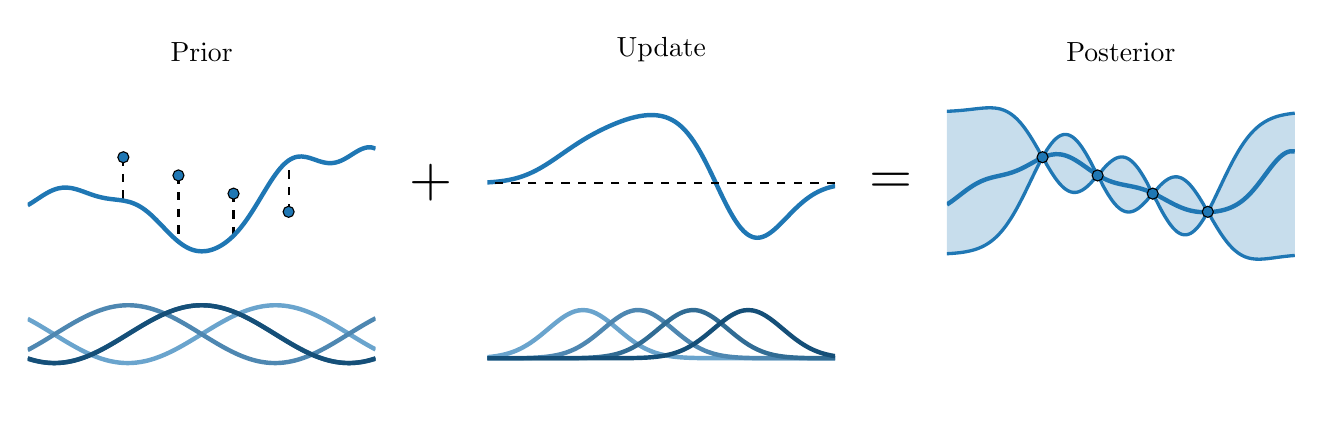
\begin{tikzpicture}
\begin{groupplot}[group style={group size={5 by 2}, horizontal sep={0pt}, vertical sep={0pt}}]
    \nextgroupplot[axis lines={none}, height={4.5cm}, width={6cm}, xmin={-0.5}, xmax={0.5}, ymin={-1}, ymax={1}, title={Prior}, title style={yshift={-0.25cm}}]
    \node at (-0.5,-1) {};
    \node at (-0.5,1) {};
    \node at (0.5,1) {};
    \node at (0.5,-1) {};
    \addplot[no markers, dashed, black, thick]
        coordinates {
            (-0.225,0.225)
            (-0.225,-0.15257176856341123)
        }
        ;
    \addplot[no markers, dashed, black, thick]
        coordinates {
            (-0.06666666666666667,0.06666666666666667)
            (-0.06666666666666667,-0.5100202088429248)
        }
        ;
    \addplot[no markers, dashed, black, thick]
        coordinates {
            (0.09166666666666666,-0.09166666666666666)
            (0.09166666666666666,-0.457645441329253)
        }
        ;
    \addplot[no markers, dashed, black, thick]
        coordinates {
            (0.25,-0.25)
            (0.25,0.1968851878679059)
        }
        ;
    \addplot[no markers, smooth, ultra thick, color={rgb,1:red,0.1216;green,0.4667;blue,0.7059}]
        coordinates {
            (-0.5,-0.19263633928580778)
            (-0.4875,-0.16969870613318833)
            (-0.475,-0.14493979183522607)
            (-0.4625,-0.11987696130162916)
            (-0.45,-0.09610010133448676)
            (-0.4375,-0.07511773789034992)
            (-0.425,-0.058210912433496985)
            (-0.4125,-0.04631083298033799)
            (-0.4,-0.03991375141564633)
            (-0.3875,-0.0390424256722741)
            (-0.375,-0.04325836250382091)
            (-0.3625,-0.05172338722072433)
            (-0.35,-0.06330359166242086)
            (-0.3375,-0.07670399527525378)
            (-0.325,-0.0906188525993171)
            (-0.3125,-0.10388083971833527)
            (-0.3,-0.1155925435451497)
            (-0.2875,-0.12522573564876063)
            (-0.275,-0.13267759733611453)
            (-0.2625,-0.13827794952745004)
            (-0.25,-0.14274706756168473)
            (-0.2375,-0.1471091938521139)
            (-0.225,-0.15257176856341118)
            (-0.2125,-0.16038412346614117)
            (-0.2,-0.17169150941617278)
            (-0.1875,-0.18740062339499314)
            (-0.175,-0.20807125005764096)
            (-0.1625,-0.23384543318636328)
            (-0.15,-0.26442113292469116)
            (-0.1375,-0.2990721382016202)
            (-0.125,-0.3367107047362433)
            (-0.1125,-0.3759846006064339)
            (-0.1,-0.41539652198610133)
            (-0.0875,-0.4534316191287965)
            (-0.075,-0.4886783938563528)
            (-0.0625,-0.5199295316339518)
            (-0.05,-0.546252136730075)
            (-0.0375,-0.5670209783162686)
            (-0.025,-0.5819132107522056)
            (-0.0125,-0.5908679987378583)
            (0.0,-0.5940189401043551)
            (0.0125,-0.5916105795745499)
            (0.025,-0.5839122185686877)
            (0.0375,-0.5711424033467826)
            (0.05,-0.5534158836045343)
            (0.0625,-0.5307216620462495)
            (0.075,-0.5029363870045327)
            (0.0875,-0.46987231366901605)
            (0.1,-0.43135400456658324)
            (0.1125,-0.38731350190313246)
            (0.125,-0.33789046602839484)
            (0.1375,-0.2835221839974399)
            (0.15,-0.22500866686677298)
            (0.1625,-0.1635403041402277)
            (0.175,-0.10067952317571781)
            (0.1875,-0.03829318810342578)
            (0.2,0.02156152724120586)
            (0.2125,0.0767890445266511)
            (0.225,0.12543101519281033)
            (0.2375,0.1658477118641975)
            (0.25,0.1968851878679058)
            (0.2625,0.21800842713147522)
            (0.275,0.22938322135002562)
            (0.2875,0.23189414043502626)
            (0.3,0.22709226762865972)
            (0.3125,0.21707370760176484)
            (0.325,0.20429746079092684)
            (0.3375,0.19135825257859834)
            (0.35,0.18073551288569722)
            (0.3625,0.17454325082489822)
            (0.375,0.17430659796602643)
            (0.3875,0.18078910382632643)
            (0.4,0.193890551601469)
            (0.4125,0.21262850238258538)
            (0.425,0.23520860652629083)
            (0.4375,0.2591797648674409)
            (0.45,0.28166140693155306)
            (0.4625,0.29962241024667025)
            (0.475,0.310185351230755)
            (0.4875,0.3109265044938405)
            (0.5,0.300141685552682)
        }
        ;
    \addplot[only marks, fill={rgb,1:red,0.1216;green,0.4667;blue,0.7059}]
        coordinates {
            (-0.225,0.225)
            (-0.06666666666666667,0.06666666666666667)
            (0.09166666666666666,-0.09166666666666666)
            (0.25,-0.25)
        }
        ;
    \nextgroupplot[axis lines={none}, height={4.5cm}, width={3cm}, xmin={-0.5}, xmax={0.5}, ymin={-1}, ymax={1}]
    \node at (-0.5,-1) {};
    \node at (-0.5,1) {};
    \node at (0.5,1) {};
    \node at (0.5,-1) {};
    \node[scale=2] at (0,0) {+};
    \nextgroupplot[axis lines={none}, height={4.5cm}, width={6cm}, xmin={-0.5}, xmax={0.5}, ymin={-1}, ymax={1}, title={Update}, title style={yshift={-0.25cm}}]
    \node at (-0.5,-1) {};
    \node at (-0.5,1) {};
    \node at (0.5,1) {};
    \node at (0.5,-1) {};
    \addplot[no markers, smooth, ultra thick, color={rgb,1:red,0.1216;green,0.4667;blue,0.7059}]
        coordinates {
            (-0.5,0.0059774728931030014)
            (-0.4875,0.008373961744483441)
            (-0.475,0.011552368055848382)
            (-0.4625,0.01569502549445799)
            (-0.45,0.021000682977140642)
            (-0.4375,0.02767711432866153)
            (-0.425,0.03593082828090464)
            (-0.4125,0.045954135274268275)
            (-0.4,0.057910245347805846)
            (-0.3875,0.07191751257038687)
            (-0.375,0.08803433781506038)
            (-0.3625,0.10624651289451487)
            (-0.35,0.12645885556470332)
            (-0.3375,0.1484927843978264)
            (-0.325,0.17209098754873844)
            (-0.3125,0.19692957175678452)
            (-0.3,0.22263711576849451)
            (-0.2875,0.2488190269111243)
            (-0.275,0.27508467893928723)
            (-0.2625,0.30107417116568297)
            (-0.25,0.3264813454608039)
            (-0.2375,0.35107001989947423)
            (-0.225,0.3746812468547982)
            (-0.2125,0.39723067739751133)
            (-0.2,0.41869661557714505)
            (-0.1875,0.4391008121323744)
            (-0.175,0.45848519592133796)
            (-0.1625,0.47688833109014467)
            (-0.15,0.49432527211008387)
            (-0.1375,0.5107736561642126)
            (-0.125,0.5261674614859683)
            (-0.1125,0.5403981417874754)
            (-0.1,0.5533211753806729)
            (-0.0875,0.5647648108860024)
            (-0.075,0.5745372522499442)
            (-0.0625,0.5824288720807421)
            (-0.05,0.5882072625985824)
            (-0.0375,0.5916048284903289)
            (-0.025,0.5923008397741214)
            (-0.0125,0.5899019486009721)
            (0.0,0.5839266810690372)
            (0.0125,0.5737999795582949)
            (0.025,0.5588632904853402)
            (0.0375,0.5384039702827027)
            (0.05,0.5117051327304292)
            (0.0625,0.4781138723139368)
            (0.075,0.4371225673343672)
            (0.0875,0.3884552114587369)
            (0.1,0.3321488971757125)
            (0.1125,0.2686199963850559)
            (0.125,0.19870538608917956)
            (0.1375,0.12367118657745284)
            (0.15,0.04518466851975817)
            (0.1625,-0.034751145378714356)
            (0.175,-0.11389658398547169)
            (0.1875,-0.18990075338097012)
            (0.2,-0.26044286621584595)
            (0.2125,-0.3233771317621039)
            (0.225,-0.3768682767405342)
            (0.2375,-0.41950558556996964)
            (0.25,-0.4503854737183366)
            (0.2625,-0.4691557857342212)
            (0.275,-0.47601886248016934)
            (0.2875,-0.47169449447905115)
            (0.3,-0.45734769447924495)
            (0.3125,-0.4344893485282862)
            (0.325,-0.4048599062338984)
            (0.3375,-0.37030715520422747)
            (0.35,-0.33266876442499227)
            (0.3625,-0.29366881100083075)
            (0.375,-0.2548351930430855)
            (0.3875,-0.21744203449536084)
            (0.4,-0.1824782906032538)
            (0.4125,-0.15064112198486754)
            (0.425,-0.12235050019089928)
            (0.4375,-0.09778010957266979)
            (0.45,-0.07689897236829642)
            (0.4625,-0.05951829110803069)
            (0.475,-0.04533863694374848)
            (0.4875,-0.033993628152892745)
            (0.5,-0.02508744111448224)
        }
        ;
    \draw[dashed, black, thick] ({rel axis cs:1,0}|-{axis cs:0,0}) -- ({rel axis cs:0,0}|-{axis cs:0,0});
    \nextgroupplot[axis lines={none}, height={4.5cm}, width={3cm}, xmin={-0.5}, xmax={0.5}, ymin={-1}, ymax={1}]
    \node at (-0.5,-1) {};
    \node at (-0.5,1) {};
    \node at (0.5,1) {};
    \node at (0.5,-1) {};
    \node[scale=2] at (0,0) {=};
    \nextgroupplot[axis lines={none}, height={4.5cm}, width={6cm}, xmin={-0.5}, xmax={0.5}, ymin={-1}, ymax={1}, title={Posterior}, title style={yshift={-0.25cm}}]
    \node at (-0.5,-1) {};
    \node at (-0.5,1) {};
    \node at (0.5,1) {};
    \node at (0.5,-1) {};
    \addplot[no markers, smooth, very thick, color={rgb,1:red,0.1216;green,0.4667;blue,0.7059}, name path={upper}]
        coordinates {
            (-0.5,0.6246794955590474)
            (-0.4875,0.626527108535127)
            (-0.475,0.6288859990663431)
            (-0.4625,0.6318054201748163)
            (-0.45,0.6352906797108888)
            (-0.4375,0.6392755475748363)
            (-0.425,0.6435904734259694)
            (-0.4125,0.6479301025420091)
            (-0.4,0.6518252831043051)
            (-0.3875,0.6546259094697102)
            (-0.375,0.6555010636128037)
            (-0.3625,0.6534617348151985)
            (-0.35,0.6474089830737757)
            (-0.3375,0.636207146515092)
            (-0.325,0.6187781345602754)
            (-0.3125,0.5942095588385343)
            (-0.3,0.5618668875530715)
            (-0.2875,0.521498289849526)
            (-0.275,0.4733206131405444)
            (-0.2625,0.41807640828704934)
            (-0.25,0.3570571885829142)
            (-0.2375,0.292122569933047)
            (-0.225,0.231175577638407)
            (-0.2125,0.2892754855192571)
            (-0.2,0.3430183327496612)
            (-0.1875,0.38443366814803337)
            (-0.175,0.411615635098621)
            (-0.1625,0.42330063040739574)
            (-0.15,0.4189196214311566)
            (-0.1375,0.3986518905136771)
            (-0.125,0.3634405899852235)
            (-0.1125,0.31496479980440784)
            (-0.1,0.25556979382740075)
            (-0.0875,0.18816748459701776)
            (-0.075,0.11622286114634428)
            (-0.0625,0.08232065964113527)
            (-0.05,0.1248188918076605)
            (-0.0375,0.16392940700865397)
            (-0.025,0.19588211675949746)
            (-0.0125,0.21782770049872327)
            (0.0,0.22754438394317988)
            (0.0125,0.22354941506243164)
            (0.025,0.20518499713199378)
            (0.0375,0.17265654177434922)
            (0.05,0.12702007676030036)
            (0.0625,0.07012291595145181)
            (0.075,0.004520206185860812)
            (0.0875,-0.06620277242209767)
            (0.1,-0.06230459899149249)
            (0.1125,-0.022026068735040955)
            (0.125,0.012348958197373222)
            (0.1375,0.03784989315296683)
            (0.15,0.05224928441106841)
            (0.1625,0.05405698275848661)
            (0.175,0.042583255508443135)
            (0.1875,0.01795586770006205)
            (0.2,-0.01891786834526299)
            (0.2125,-0.06644080066488525)
            (0.225,-0.12245556352324188)
            (0.2375,-0.18436716318637397)
            (0.25,-0.2437780598378386)
            (0.2625,-0.17715766485922416)
            (0.275,-0.09975423488117821)
            (0.2875,-0.01996553090088618)
            (0.3,0.05958220137092163)
            (0.3125,0.13661317083999797)
            (0.325,0.20925181834233292)
            (0.3375,0.27607610731553195)
            (0.35,0.3361372413900543)
            (0.3625,0.3889437051088219)
            (0.375,0.4344140979048779)
            (0.3875,0.4728065448828661)
            (0.4,0.5046343262180886)
            (0.4125,0.5305778701306155)
            (0.425,0.5514023967679502)
            (0.4375,0.5678884312981339)
            (0.45,0.5807794997380554)
            (0.4625,0.5907481561974323)
            (0.475,0.5983787107455051)
            (0.4875,0.6041631507690505)
            (0.5,0.6085059964063713)
        }
        ;
    \addplot[no markers, smooth, very thick, color={rgb,1:red,0.1216;green,0.4667;blue,0.7059}, name path={lower}]
        coordinates {
            (-0.5,-0.6145809860556101)
            (-0.4875,-0.6123960907471674)
            (-0.475,-0.6094185878014922)
            (-0.4625,-0.605401857573206)
            (-0.45,-0.6000343093563807)
            (-0.4375,-0.5929271367885144)
            (-0.425,-0.5836036290842439)
            (-0.4125,-0.5714931748018549)
            (-0.4,-0.5559340201829982)
            (-0.3875,-0.536189132523361)
            (-0.375,-0.511478802295605)
            (-0.3625,-0.4810317681905123)
            (-0.35,-0.4441538811724856)
            (-0.3375,-0.4003101492641122)
            (-0.325,-0.3492130663661145)
            (-0.3125,-0.29090800209722073)
            (-0.3,-0.22584549578551621)
            (-0.2875,-0.1549307146697954)
            (-0.275,-0.07954211066510897)
            (-0.2625,-0.0015145554420807894)
            (-0.25,0.07691123180945425)
            (-0.2375,0.1531361682474075)
            (-0.225,0.21878012884446243)
            (-0.2125,0.15860219621031357)
            (-0.2,0.09613014648803336)
            (-0.1875,0.03974956488581821)
            (-0.175,-0.007963937421260892)
            (-0.1625,-0.04487763054293023)
            (-0.15,-0.06942190532200179)
            (-0.1375,-0.08071766848900602)
            (-0.125,-0.07866417644207363)
            (-0.1125,-0.06397562942826043)
            (-0.1,-0.03816331373452023)
            (-0.0875,-0.003472254988527282)
            (-0.075,0.037112750774538246)
            (-0.0625,0.041296538045874444)
            (-0.05,-0.029170653475929162)
            (-0.0375,-0.09455454203204541)
            (-0.025,-0.15127553374016106)
            (-0.0125,-0.19678291435958475)
            (0.0,-0.2292325974277668)
            (0.0125,-0.24757053486777103)
            (0.025,-0.2515919842389529)
            (0.0375,-0.2419540730839588)
            (0.05,-0.22013757373935816)
            (0.0625,-0.18836103308924795)
            (0.075,-0.14946933909772886)
            (0.0875,-0.1072268940173559)
            (0.1,-0.14141470936329986)
            (0.1125,-0.2136658083205849)
            (0.125,-0.2813841493645485)
            (0.1375,-0.34109053607970197)
            (0.15,-0.3898554820162277)
            (0.1625,-0.42531257624419627)
            (0.175,-0.445758271244715)
            (0.1875,-0.45022239325026414)
            (0.2,-0.4384974408651446)
            (0.2125,-0.4111249039271001)
            (0.225,-0.3693437497848697)
            (0.2375,-0.3150404524953183)
            (0.25,-0.2561735086317917)
            (0.2625,-0.3161440665448644)
            (0.275,-0.37990019165463884)
            (0.2875,-0.439556494630016)
            (0.3,-0.49328052243473197)
            (0.3125,-0.5398158336793233)
            (0.325,-0.5784605649962549)
            (0.3375,-0.6090414536202231)
            (0.35,-0.6318539595363356)
            (0.3625,-0.6475735906703822)
            (0.375,-0.6571487663413834)
            (0.3875,-0.6616869581228447)
            (0.4,-0.6623455396903202)
            (0.4125,-0.6602371718624557)
            (0.425,-0.6563569065193531)
            (0.4375,-0.6515348460457301)
            (0.45,-0.6464146027721579)
            (0.4625,-0.6414545281659184)
            (0.475,-0.6369462783217644)
            (0.4875,-0.6330441269789718)
            (0.5,-0.629798590461464)
        }
        ;
    \addplot[color={rgb,1:red,0.1216;green,0.4667;blue,0.7059}, opacity={0.25}]
        fill between [of = upper and lower]
        ;
    \addplot[no markers, smooth, ultra thick, color={rgb,1:red,0.1216;green,0.4667;blue,0.7059}]
        coordinates {
            (-0.5,-0.1866588663927048)
            (-0.4875,-0.1613247443887049)
            (-0.475,-0.13338742377937768)
            (-0.4625,-0.10418193580717117)
            (-0.45,-0.07509941835734613)
            (-0.4375,-0.04744062356168839)
            (-0.425,-0.022280084152592347)
            (-0.4125,-0.0003566977060697127)
            (-0.4,0.01799649393215952)
            (-0.3875,0.03287508689811276)
            (-0.375,0.044775975311239474)
            (-0.3625,0.054523125673790536)
            (-0.35,0.06315526390228246)
            (-0.3375,0.07178878912257262)
            (-0.325,0.08147213494942135)
            (-0.3125,0.09304873203844925)
            (-0.3,0.10704457222334482)
            (-0.2875,0.12359329126236368)
            (-0.275,0.1424070816031727)
            (-0.2625,0.16279622163823293)
            (-0.25,0.18373427789911914)
            (-0.2375,0.20396082604736032)
            (-0.225,0.22210947829138702)
            (-0.2125,0.23684655393137016)
            (-0.2,0.24700510616097227)
            (-0.1875,0.25170018873738126)
            (-0.175,0.25041394586369703)
            (-0.1625,0.2430428979037814)
            (-0.15,0.2299041391853927)
            (-0.1375,0.21170151796259234)
            (-0.125,0.18945675674972495)
            (-0.1125,0.16441354118104146)
            (-0.1,0.1379246533945716)
            (-0.0875,0.11133319175720591)
            (-0.075,0.08585885839359142)
            (-0.0625,0.062499340446790286)
            (-0.05,0.04195512586850736)
            (-0.0375,0.024583850174060284)
            (-0.025,0.010387629021915812)
            (-0.0125,-0.0009660501368862207)
            (0.0,-0.010092259035317852)
            (0.0125,-0.017810600016255007)
            (0.025,-0.025048928083347466)
            (0.0375,-0.032738433064079864)
            (0.05,-0.04171075087410514)
            (0.0625,-0.05260778973231267)
            (0.075,-0.06581381967016547)
            (0.0875,-0.08141710221027915)
            (0.1,-0.09920510739087074)
            (0.1125,-0.11869350551807656)
            (0.125,-0.13918507993921528)
            (0.1375,-0.15985099741998704)
            (0.15,-0.17982399834701482)
            (0.1625,-0.19829144951894204)
            (0.175,-0.2145761071611895)
            (0.1875,-0.2281939414843959)
            (0.2,-0.2388813389746401)
            (0.2125,-0.24658808723545284)
            (0.225,-0.25143726154772383)
            (0.2375,-0.25365787370577214)
            (0.25,-0.25350028585043083)
            (0.2625,-0.25114735860274595)
            (0.275,-0.24663564113014372)
            (0.2875,-0.2398003540440249)
            (0.3,-0.23025542685058523)
            (0.3125,-0.21741564092652135)
            (0.325,-0.20056244544297155)
            (0.3375,-0.17894890262562912)
            (0.35,-0.15193325153929504)
            (0.3625,-0.11912556017593254)
            (0.375,-0.08052859507705906)
            (0.3875,-0.03665293066903441)
            (0.4,0.011412260998215212)
            (0.4125,0.06198738039771784)
            (0.425,0.11285810633539155)
            (0.4375,0.16139965529477107)
            (0.45,0.20476243456325666)
            (0.4625,0.24010411913863955)
            (0.475,0.26484671428700657)
            (0.4875,0.27693287634094776)
            (0.5,0.27505424443819976)
        }
        ;
    \addplot[only marks, fill={rgb,1:red,0.1216;green,0.4667;blue,0.7059}]
        coordinates {
            (-0.225,0.225)
            (-0.06666666666666667,0.06666666666666667)
            (0.09166666666666666,-0.09166666666666666)
            (0.25,-0.25)
        }
        ;
    \nextgroupplot[axis lines={none}, height={2.5cm}, width={6cm}, xmin={-0.5}, xmax={0.5}, ymin={-1.25}, ymax={1.25}]
    \node at (-0.5,-1.25) {};
    \node at (-0.5,1.25) {};
    \node at (0.5,1.25) {};
    \node at (0.5,-1.25) {};
    \addplot[no markers, smooth, ultra thick, color={rgb,1:red,0.4157;green,0.6431;blue,0.8039}]
        coordinates {
            (-0.5,0.5282265970259133)
            (-0.4875,0.44758067935444945)
            (-0.475,0.3631117989963583)
            (-0.4625,0.27554143789374724)
            (-0.45,0.18561756895606404)
            (-0.4375,0.094108267329184)
            (-0.425,0.0017951499633817273)
            (-0.4125,-0.09053330048457416)
            (-0.4,-0.18208847039202697)
            (-0.3875,-0.2720883510296714)
            (-0.375,-0.3597642180057953)
            (-0.3625,-0.44436719724377227)
            (-0.35,-0.5251746614102)
            (-0.3375,-0.6014964021592782)
            (-0.325,-0.6726805254738597)
            (-0.3125,-0.7381190197487418)
            (-0.3,-0.7972529490570146)
            (-0.2875,-0.8495772272417301)
            (-0.275,-0.8946449320554997)
            (-0.2625,-0.932071122499254)
            (-0.25,-0.9615361267547736)
            (-0.2375,-0.982788272627466)
            (-0.225,-0.9956460371776034)
            (-0.2125,-0.9999995971791705)
            (-0.2,-0.9958117671632505)
            (-0.1875,-0.9831183170337451)
            (-0.175,-0.9620276665425517)
            (-0.1625,-0.9327199592338037)
            (-0.15,-0.8954455237669809)
            (-0.1375,-0.8505227357613357)
            (-0.125,-0.7983352984244607)
            (-0.1125,-0.7393289651922219)
            (-0.1,-0.6740077323732784)
            (-0.0875,-0.6029295343183069)
            (-0.075,-0.5267014778831904)
            (-0.0625,-0.4459746568904911)
            (-0.05,-0.36143859088093155)
            (-0.0375,-0.27381533565570293)
            (-0.025,-0.1838533159137668)
            (-0.0125,-0.09232093266202773)
            (0.0,0.0)
            (0.0125,0.09232093266202773)
            (0.025,0.1838533159137668)
            (0.0375,0.27381533565570293)
            (0.05,0.36143859088093155)
            (0.0625,0.4459746568904911)
            (0.075,0.5267014778831904)
            (0.0875,0.6029295343183069)
            (0.1,0.6740077323732784)
            (0.1125,0.7393289651922219)
            (0.125,0.7983352984244607)
            (0.1375,0.8505227357613357)
            (0.15,0.8954455237669809)
            (0.1625,0.9327199592338037)
            (0.175,0.9620276665425517)
            (0.1875,0.9831183170337451)
            (0.2,0.9958117671632505)
            (0.2125,0.9999995971791705)
            (0.225,0.9956460371776034)
            (0.2375,0.982788272627466)
            (0.25,0.9615361267547736)
            (0.2625,0.932071122499254)
            (0.275,0.8946449320554997)
            (0.2875,0.8495772272417301)
            (0.3,0.7972529490570146)
            (0.3125,0.7381190197487418)
            (0.325,0.6726805254738597)
            (0.3375,0.6014964021592782)
            (0.35,0.5251746614102)
            (0.3625,0.44436719724377227)
            (0.375,0.3597642180057953)
            (0.3875,0.2720883510296714)
            (0.4,0.18208847039202697)
            (0.4125,0.09053330048457416)
            (0.425,-0.0017951499633817273)
            (0.4375,-0.094108267329184)
            (0.45,-0.18561756895606404)
            (0.4625,-0.27554143789374724)
            (0.475,-0.3631117989963583)
            (0.4875,-0.44758067935444945)
            (0.5,-0.5282265970259133)
        }
        ;
    \addplot[no markers, smooth, ultra thick, color={rgb,1:red,0.3059;green,0.5294;blue,0.6941}]
        coordinates {
            (-0.5,-0.5488123578445427)
            (-0.4875,-0.46875381758088513)
            (-0.475,-0.38463842623055305)
            (-0.4625,-0.29719416424726647)
            (-0.45,-0.20717782194599482)
            (-0.4375,-0.11536844982699483)
            (-0.425,-0.022560616248067246)
            (-0.4125,0.07044246920318549)
            (-0.4,0.16283590712301116)
            (-0.3875,0.2538200743297558)
            (-0.375,0.34260754423880496)
            (-0.3625,0.4284299016815255)
            (-0.35,0.5105443931890508)
            (-0.3375,0.588240355185726)
            (-0.325,0.6608453644591219)
            (-0.3125,0.7277310576770969)
            (-0.3,0.7883185695866395)
            (-0.2875,0.8420835428293442)
            (-0.275,0.888560666015854)
            (-0.2625,0.927347700784298)
            (-0.25,0.9581089629903607)
            (-0.2375,0.9805782279008713)
            (-0.225,0.9945610342477823)
            (-0.2125,0.9999363672019963)
            (-0.2,0.996657705701671)
            (-0.1875,0.9847534250708497)
            (-0.175,0.9643265514439381)
            (-0.1625,0.9355538701213703)
            (-0.15,0.8986843955732415)
            (-0.1375,0.8540372163323293)
            (-0.125,0.8019987334279738)
            (-0.1125,0.7430193162609172)
            (-0.1,0.6776094048609824)
            (-0.0875,0.60633509226078)
            (-0.075,0.5298132252179883)
            (-0.0625,0.44870606568722793)
            (-0.05,0.3637155592440624)
            (-0.0375,0.2755772600653098)
            (-0.025,0.18505396504219604)
            (-0.0125,0.09292911212020634)
            (0.0,-0.0)
            (0.0125,-0.09292911212020634)
            (0.025,-0.18505396504219604)
            (0.0375,-0.2755772600653098)
            (0.05,-0.3637155592440624)
            (0.0625,-0.44870606568722793)
            (0.075,-0.5298132252179883)
            (0.0875,-0.60633509226078)
            (0.1,-0.6776094048609824)
            (0.1125,-0.7430193162609172)
            (0.125,-0.8019987334279738)
            (0.1375,-0.8540372163323293)
            (0.15,-0.8986843955732415)
            (0.1625,-0.9355538701213703)
            (0.175,-0.9643265514439381)
            (0.1875,-0.9847534250708497)
            (0.2,-0.996657705701671)
            (0.2125,-0.9999363672019963)
            (0.225,-0.9945610342477823)
            (0.2375,-0.9805782279008713)
            (0.25,-0.9581089629903607)
            (0.2625,-0.927347700784298)
            (0.275,-0.888560666015854)
            (0.2875,-0.8420835428293442)
            (0.3,-0.7883185695866395)
            (0.3125,-0.7277310576770969)
            (0.325,-0.6608453644591219)
            (0.3375,-0.588240355185726)
            (0.35,-0.5105443931890508)
            (0.3625,-0.4284299016815255)
            (0.375,-0.34260754423880496)
            (0.3875,-0.2538200743297558)
            (0.4,-0.16283590712301116)
            (0.4125,-0.07044246920318549)
            (0.425,0.022560616248067246)
            (0.4375,0.11536844982699483)
            (0.45,0.20717782194599482)
            (0.4625,0.29719416424726647)
            (0.475,0.38463842623055305)
            (0.4875,0.46875381758088513)
            (0.5,0.5488123578445427)
        }
        ;
    \addplot[no markers, smooth, ultra thick, color={rgb,1:red,0.1922;green,0.4235;blue,0.5804}]
        coordinates {
            (-0.5,-0.8491034461091436)
            (-0.4875,-0.8942435548935254)
            (-0.475,-0.9317455776281574)
            (-0.4625,-0.9612891947813864)
            (-0.45,-0.9826220626949309)
            (-0.4375,-0.9955619689503505)
            (-0.425,-0.9999983887170064)
            (-0.4125,-0.9958934287881259)
            (-0.4,-0.9832821512415916)
            (-0.3875,-0.962272273960938)
            (-0.375,-0.9330432505745265)
            (-0.3625,-0.8958447376714976)
            (-0.35,-0.8509944623866139)
            (-0.3375,-0.7988755085677893)
            (-0.325,-0.7399330447062167)
            (-0.3125,-0.6746705215771298)
            (-0.3,-0.6036453720686454)
            (-0.2875,-0.5274642499281383)
            (-0.275,-0.44677784809389365)
            (-0.2625,-0.36227534087069846)
            (-0.25,-0.2746784974209452)
            (-0.2375,-0.18473551685022943)
            (-0.225,-0.09321463754440355)
            (-0.2125,-0.0008975753432529078)
            (-0.2,0.09142715340206255)
            (-0.1875,0.18297096685741362)
            (-0.175,0.27295195329341954)
            (-0.1625,0.36060154970117875)
            (-0.15,0.445171106391326)
            (-0.1375,0.52593828150559)
            (-0.125,0.6022132108228178)
            (-0.1125,0.6733444001607188)
            (-0.1,0.7387242900440132)
            (-0.0875,0.7977944451089577)
            (-0.075,0.8500503239195095)
            (-0.0625,0.8950455884542469)
            (-0.05,0.9323959164550254)
            (-0.0375,0.9617822840746001)
            (-0.025,0.9829536907848268)
            (-0.0125,0.9957293032709308)
            (0.0,1.0)
            (0.0125,0.9957293032709308)
            (0.025,0.9829536907848268)
            (0.0375,0.9617822840746001)
            (0.05,0.9323959164550254)
            (0.0625,0.8950455884542469)
            (0.075,0.8500503239195095)
            (0.0875,0.7977944451089577)
            (0.1,0.7387242900440132)
            (0.1125,0.6733444001607188)
            (0.125,0.6022132108228178)
            (0.1375,0.52593828150559)
            (0.15,0.445171106391326)
            (0.1625,0.36060154970117875)
            (0.175,0.27295195329341954)
            (0.1875,0.18297096685741362)
            (0.2,0.09142715340206255)
            (0.2125,-0.0008975753432529078)
            (0.225,-0.09321463754440355)
            (0.2375,-0.18473551685022943)
            (0.25,-0.2746784974209452)
            (0.2625,-0.36227534087069846)
            (0.275,-0.44677784809389365)
            (0.2875,-0.5274642499281383)
            (0.3,-0.6036453720686454)
            (0.3125,-0.6746705215771298)
            (0.325,-0.7399330447062167)
            (0.3375,-0.7988755085677893)
            (0.35,-0.8509944623866139)
            (0.3625,-0.8958447376714976)
            (0.375,-0.9330432505745265)
            (0.3875,-0.962272273960938)
            (0.4,-0.9832821512415916)
            (0.4125,-0.9958934287881259)
            (0.425,-0.9999983887170064)
            (0.4375,-0.9955619689503505)
            (0.45,-0.9826220626949309)
            (0.4625,-0.9612891947813864)
            (0.475,-0.9317455776281574)
            (0.4875,-0.8942435548935254)
            (0.5,-0.8491034461091436)
        }
        ;
    \addplot[no markers, smooth, ultra thick, color={rgb,1:red,0.0824;green,0.3098;blue,0.4706}]
        coordinates {
            (-0.5,-0.8359455699249285)
            (-0.4875,-0.8833288507137906)
            (-0.475,-0.9230673220664262)
            (-0.4625,-0.954817065587628)
            (-0.45,-0.9783033016880367)
            (-0.4375,-0.9933227676765072)
            (-0.425,-0.9997454769062512)
            (-0.4125,-0.9975158437501422)
            (-0.4,-0.9866531646690372)
            (-0.3875,-0.9672514512096828)
            (-0.375,-0.9394786163775393)
            (-0.3625,-0.9035750214260897)
            (-0.35,-0.8598513956395164)
            (-0.3375,-0.8086861471120739)
            (-0.325,-0.7505220877981476)
            (-0.3125,-0.6858626011761932)
            (-0.3,-0.6152672856936849)
            (-0.2875,-0.5393471116970778)
            (-0.275,-0.4587591337613476)
            (-0.2625,-0.37420080418149304)
            (-0.25,-0.2864039368401484)
            (-0.2375,-0.19612837369128136)
            (-0.225,-0.10415540867368181)
            (-0.2125,-0.011281025967280273)
            (-0.2,0.08169098888789043)
            (-0.1875,0.1739560053899561)
            (-0.175,0.2647155117862228)
            (-0.1625,0.3531840258292074)
            (-0.15,0.43859589276822636)
            (-0.1375,0.5202119117430186)
            (-0.125,0.5973257332309783)
            (-0.1125,0.6692699721810019)
            (-0.1,0.7354219839275579)
            (-0.0875,0.795209252897067)
            (-0.075,0.8481143474697932)
            (-0.0625,0.893679398115168)
            (-0.05,0.9315100600443234)
            (-0.0375,0.9612789260848782)
            (-0.025,0.9827283602411002)
            (-0.0125,0.9956727274162681)
            (0.0,1.0)
            (0.0125,0.9956727274162681)
            (0.025,0.9827283602411002)
            (0.0375,0.9612789260848782)
            (0.05,0.9315100600443234)
            (0.0625,0.893679398115168)
            (0.075,0.8481143474697932)
            (0.0875,0.795209252897067)
            (0.1,0.7354219839275579)
            (0.1125,0.6692699721810019)
            (0.125,0.5973257332309783)
            (0.1375,0.5202119117430186)
            (0.15,0.43859589276822636)
            (0.1625,0.3531840258292074)
            (0.175,0.2647155117862228)
            (0.1875,0.1739560053899561)
            (0.2,0.08169098888789043)
            (0.2125,-0.011281025967280273)
            (0.225,-0.10415540867368181)
            (0.2375,-0.19612837369128136)
            (0.25,-0.2864039368401484)
            (0.2625,-0.37420080418149304)
            (0.275,-0.4587591337613476)
            (0.2875,-0.5393471116970778)
            (0.3,-0.6152672856936849)
            (0.3125,-0.6858626011761932)
            (0.325,-0.7505220877981476)
            (0.3375,-0.8086861471120739)
            (0.35,-0.8598513956395164)
            (0.3625,-0.9035750214260897)
            (0.375,-0.9394786163775393)
            (0.3875,-0.9672514512096828)
            (0.4,-0.9866531646690372)
            (0.4125,-0.9975158437501422)
            (0.425,-0.9997454769062512)
            (0.4375,-0.9933227676765072)
            (0.45,-0.9783033016880367)
            (0.4625,-0.954817065587628)
            (0.475,-0.9230673220664262)
            (0.4875,-0.8833288507137906)
            (0.5,-0.8359455699249285)
        }
        ;
    \nextgroupplot[axis lines={none}, height={3cm}, width={3cm}, xmin={-0.5}, xmax={0.5}, ymin={-1}, ymax={1}]
    \node at (-0.5,-1) {};
    \node at (-0.5,1) {};
    \node at (0.5,1) {};
    \node at (0.5,-1) {};
    \nextgroupplot[axis lines={none}, height={2.5cm}, width={6cm}, xmin={-0.5}, xmax={0.5}, ymin={-0.025}, ymax={0.125}]
    \node at (0,-0.025) {};
    \node at (0,0.125) {};
    \node at (1,0.125) {};
    \node at (1,-0.025) {};
    \addplot[no markers, smooth, ultra thick, color={rgb,1:red,0.4157;green,0.6431;blue,0.8039}]
        coordinates {
            (-0.5,0.0022794180883612346)
            (-0.4875,0.00318947933621571)
            (-0.475,0.004393693362340742)
            (-0.4625,0.0059587318761986086)
            (-0.45,0.007955950871822768)
            (-0.4375,0.010457900128900147)
            (-0.425,0.013533528323661271)
            (-0.4125,0.017242162389375284)
            (-0.4,0.021626516682988733)
            (-0.3875,0.026705183522634336)
            (-0.375,0.03246524673583497)
            (-0.3625,0.03885581275123642)
            (-0.35,0.04578333617716143)
            (-0.3375,0.05310959910353452)
            (-0.325,0.06065306597126335)
            (-0.3125,0.06819407511903482)
            (-0.3,0.07548396019890075)
            (-0.2875,0.08225775623986648)
            (-0.275,0.08824969025845955)
            (-0.2625,0.09321024923595277)
            (-0.25,0.09692332344763442)
            (-0.2375,0.09922179382602436)
            (-0.225,0.1)
            (-0.2125,0.09922179382602436)
            (-0.2,0.09692332344763442)
            (-0.1875,0.09321024923595277)
            (-0.175,0.08824969025845955)
            (-0.1625,0.08225775623986648)
            (-0.15,0.07548396019890075)
            (-0.1375,0.06819407511903482)
            (-0.125,0.06065306597126335)
            (-0.1125,0.05310959910353452)
            (-0.1,0.04578333617716143)
            (-0.0875,0.03885581275123642)
            (-0.075,0.03246524673583497)
            (-0.0625,0.026705183522634336)
            (-0.05,0.021626516682988733)
            (-0.0375,0.017242162389375284)
            (-0.025,0.013533528323661271)
            (-0.0125,0.010457900128900147)
            (0.0,0.007955950871822768)
            (0.0125,0.0059587318761986086)
            (0.025,0.004393693362340742)
            (0.0375,0.00318947933621571)
            (0.05,0.0022794180883612346)
            (0.0625,0.0016037709275350549)
            (0.075,0.0011108996538242307)
            (0.0875,0.0007575677444259936)
            (0.1,0.0005086069231012701)
            (0.1125,0.00033616864879322566)
            (0.125,0.00021874911181828853)
            (0.1375,0.00014013594188853922)
            (0.15,8.8382630693505e-5)
            (0.1625,5.487802334320488e-5)
            (0.175,3.354626279025119e-5)
            (0.1875,2.018849656009158e-5)
            (0.2,1.1961288358102437e-5)
            (0.2125,6.97695771959971e-6)
            (0.225,4.006529739295107e-6)
            (0.2375,2.265086538322931e-6)
            (0.25,1.2607105177048523e-6)
            (0.2625,6.908123638278764e-7)
            (0.275,3.726653172078671e-7)
            (0.2875,1.9792105596701347e-7)
            (0.3,1.0348542111093754e-7)
            (0.3125,5.326972955014612e-8)
            (0.325,2.6995785033630143e-8)
            (0.3375,1.3468696888087106e-8)
            (0.35,6.615601637697701e-9)
            (0.3625,3.1990959170068973e-9)
            (0.375,1.522997974471263e-9)
            (0.3875,7.138147842919371e-10)
            (0.4,3.293714110306081e-10)
            (0.4125,1.496237071043946e-10)
            (0.425,6.691586091292782e-11)
            (0.4375,2.946265481618801e-11)
            (0.45,1.2771115545128335e-11)
            (0.4625,5.450043132884139e-12)
            (0.475,2.289734845645553e-12)
            (0.4875,9.470754871762952e-13)
            (0.5,3.8565427284697243e-13)
        }
        ;
    \addplot[no markers, smooth, ultra thick, color={rgb,1:red,0.3059;green,0.5294;blue,0.6941}]
        coordinates {
            (-0.5,8.364834722972752e-6)
            (-0.4875,1.4266166326725154e-5)
            (-0.475,2.395363074928571e-5)
            (-0.4625,3.959584054817061e-5)
            (-0.45,6.443798205686087e-5)
            (-0.4375,0.00010324010680846945)
            (-0.425,0.00016284300482412124)
            (-0.4125,0.0002528738487285179)
            (-0.4,0.0003865920139472808)
            (-0.3875,0.0005818566293615982)
            (-0.375,0.0008621706688299524)
            (-0.3625,0.0012577219776965607)
            (-0.35,0.0018063013419781276)
            (-0.3375,0.0025539354003381925)
            (-0.325,0.0035550340114781096)
            (-0.3125,0.004871825910431922)
            (-0.3,0.006572852861653048)
            (-0.2875,0.00873032092577102)
            (-0.275,0.01141617600096869)
            (-0.2625,0.01469688348913193)
            (-0.25,0.018627046369770087)
            (-0.2375,0.023242181527667105)
            (-0.225,0.02855117136383191)
            (-0.2125,0.03452908907714338)
            (-0.2,0.041111229050718734)
            (-0.1875,0.04818922574296569)
            (-0.175,0.05561008837732086)
            (-0.1625,0.06317879970040398)
            (-0.15,0.07066482778577163)
            (-0.1375,0.07781250340612625)
            (-0.125,0.08435476490642344)
            (-0.1125,0.09002932618608445)
            (-0.1,0.09459594689067655)
            (-0.0875,0.09785323920732278)
            (-0.075,0.09965337989703692)
            (-0.0625,0.09991323210956757)
            (-0.05,0.09862071167439163)
            (-0.0375,0.09583571886519543)
            (-0.025,0.0916855355732029)
            (-0.0125,0.08635518050833185)
            (0.0,0.08007374029168081)
            (0.0125,0.07309808214993307)
            (0.025,0.06569555696492685)
            (0.0375,0.05812730178734145)
            (0.05,0.05063356166481006)
            (0.0625,0.04342211168096995)
            (0.075,0.03666042970736738)
            (0.0875,0.030471814159646633)
            (0.1,0.024935220877729623)
            (0.1125,0.020088257969956246)
            (0.125,0.015932557073921532)
            (0.1375,0.012440643286396783)
            (0.15,0.009563444483253861)
            (0.1625,0.007237690258523848)
            (0.175,0.005392619703062286)
            (0.1875,0.003955612528798087)
            (0.2,0.002856550078455038)
            (0.2125,0.00203087918854474)
            (0.225,0.0014214791206736985)
            (0.2375,0.0009795148611161974)
            (0.25,0.0006645011282741399)
            (0.2625,0.000443807425834459)
            (0.275,0.0002918149619400942)
            (0.2875,0.00018890119037105564)
            (0.3,0.0001203859994828203)
            (0.3125,7.553207567519686e-5)
            (0.325,4.665530201723777e-5)
            (0.3375,2.8371659521251485e-5)
            (0.35,1.6985667656141068e-5)
            (0.3625,1.001139631974864e-5)
            (0.375,5.809260270742294e-6)
            (0.3875,3.31864779537931e-6)
            (0.4,1.8664469113520602e-6)
            (0.4125,1.0334376225181898e-6)
            (0.425,5.633354002903874e-7)
            (0.4375,3.0231797326023857e-7)
            (0.45,1.5972578828343163e-7)
            (0.4625,8.308072191756636e-8)
            (0.475,4.254412850701844e-8)
            (0.4875,2.1448313589135484e-8)
            (0.5,1.0645371411076064e-8)
        }
        ;
    \addplot[no markers, smooth, ultra thick, color={rgb,1:red,0.1922;green,0.4235;blue,0.5804}]
        coordinates {
            (-0.5,2.502295527884942e-9)
            (-0.4875,5.201668060759519e-9)
            (-0.475,1.0645371411076024e-8)
            (-0.4625,2.1448313589135484e-8)
            (-0.45,4.2544128507018366e-8)
            (-0.4375,8.308072191756621e-8)
            (-0.425,1.5972578828343163e-7)
            (-0.4125,3.0231797326023804e-7)
            (-0.4,5.633354002903863e-7)
            (-0.3875,1.0334376225181898e-6)
            (-0.375,1.8664469113520572e-6)
            (-0.3625,3.31864779537931e-6)
            (-0.35,5.809260270742294e-6)
            (-0.3375,1.001139631974864e-5)
            (-0.325,1.6985667656141068e-5)
            (-0.3125,2.8371659521251485e-5)
            (-0.3,4.665530201723777e-5)
            (-0.2875,7.553207567519686e-5)
            (-0.275,0.0001203859994828203)
            (-0.2625,0.00018890119037105564)
            (-0.25,0.0002918149619400942)
            (-0.2375,0.00044380742583445933)
            (-0.225,0.0006645011282741399)
            (-0.2125,0.0009795148611161974)
            (-0.2,0.0014214791206736985)
            (-0.1875,0.00203087918854474)
            (-0.175,0.002856550078455038)
            (-0.1625,0.003955612528798087)
            (-0.15,0.005392619703062286)
            (-0.1375,0.007237690258523848)
            (-0.125,0.009563444483253861)
            (-0.1125,0.012440643286396783)
            (-0.1,0.01593255707392154)
            (-0.0875,0.020088257969956252)
            (-0.075,0.024935220877729623)
            (-0.0625,0.030471814159646633)
            (-0.05,0.03666042970736739)
            (-0.0375,0.04342211168096995)
            (-0.025,0.05063356166481007)
            (-0.0125,0.05812730178734145)
            (0.0,0.06569555696492685)
            (0.0125,0.07309808214993307)
            (0.025,0.08007374029168081)
            (0.0375,0.08635518050833185)
            (0.05,0.0916855355732029)
            (0.0625,0.09583571886519543)
            (0.075,0.09862071167439163)
            (0.0875,0.09991323210956757)
            (0.1,0.09965337989703692)
            (0.1125,0.09785323920732279)
            (0.125,0.09459594689067655)
            (0.1375,0.09002932618608443)
            (0.15,0.08435476490642346)
            (0.1625,0.07781250340612625)
            (0.175,0.07066482778577163)
            (0.1875,0.06317879970040399)
            (0.2,0.05561008837732087)
            (0.2125,0.04818922574296569)
            (0.225,0.04111122905071875)
            (0.2375,0.03452908907714338)
            (0.25,0.02855117136383191)
            (0.2625,0.02324218152766711)
            (0.275,0.01862704636977008)
            (0.2875,0.014696883489131922)
            (0.3,0.01141617600096869)
            (0.3125,0.008730320925771015)
            (0.325,0.006572852861653045)
            (0.3375,0.004871825910431922)
            (0.35,0.0035550340114781083)
            (0.3625,0.002553935400338191)
            (0.375,0.0018063013419781276)
            (0.3875,0.0012577219776965596)
            (0.4,0.0008621706688299517)
            (0.4125,0.0005818566293615982)
            (0.425,0.00038659201394728045)
            (0.4375,0.0002528738487285174)
            (0.45,0.0001628430048241211)
            (0.4625,0.00010324010680846936)
            (0.475,6.443798205686077e-5)
            (0.4875,3.959584054817058e-5)
            (0.5,2.3953630749285666e-5)
        }
        ;
    \addplot[no markers, smooth, ultra thick, color={rgb,1:red,0.0824;green,0.3098;blue,0.4706}]
        coordinates {
            (-0.5,6.101936677605324e-14)
            (-0.4875,1.546058232366766e-13)
            (-0.475,3.8565427284697243e-13)
            (-0.4625,9.470754871762952e-13)
            (-0.45,2.289734845645553e-12)
            (-0.4375,5.450043132884139e-12)
            (-0.425,1.2771115545128335e-11)
            (-0.4125,2.946265481618801e-11)
            (-0.4,6.691586091292782e-11)
            (-0.3875,1.496237071043946e-10)
            (-0.375,3.293714110306081e-10)
            (-0.3625,7.138147842919371e-10)
            (-0.35,1.522997974471263e-9)
            (-0.3375,3.1990959170068973e-9)
            (-0.325,6.615601637697701e-9)
            (-0.3125,1.3468696888087106e-8)
            (-0.3,2.6995785033630143e-8)
            (-0.2875,5.326972955014612e-8)
            (-0.275,1.0348542111093754e-7)
            (-0.2625,1.9792105596701347e-7)
            (-0.25,3.726653172078671e-7)
            (-0.2375,6.908123638278764e-7)
            (-0.225,1.2607105177048523e-6)
            (-0.2125,2.265086538322931e-6)
            (-0.2,4.006529739295107e-6)
            (-0.1875,6.97695771959971e-6)
            (-0.175,1.1961288358102437e-5)
            (-0.1625,2.018849656009158e-5)
            (-0.15,3.354626279025119e-5)
            (-0.1375,5.487802334320488e-5)
            (-0.125,8.8382630693505e-5)
            (-0.1125,0.00014013594188853922)
            (-0.1,0.00021874911181828853)
            (-0.0875,0.00033616864879322566)
            (-0.075,0.0005086069231012701)
            (-0.0625,0.0007575677444259936)
            (-0.05,0.0011108996538242307)
            (-0.0375,0.0016037709275350549)
            (-0.025,0.0022794180883612346)
            (-0.0125,0.00318947933621571)
            (0.0,0.004393693362340742)
            (0.0125,0.0059587318761986086)
            (0.025,0.007955950871822768)
            (0.0375,0.010457900128900147)
            (0.05,0.013533528323661271)
            (0.0625,0.017242162389375284)
            (0.075,0.021626516682988733)
            (0.0875,0.026705183522634336)
            (0.1,0.03246524673583497)
            (0.1125,0.03885581275123642)
            (0.125,0.04578333617716143)
            (0.1375,0.05310959910353452)
            (0.15,0.06065306597126335)
            (0.1625,0.06819407511903482)
            (0.175,0.07548396019890075)
            (0.1875,0.08225775623986648)
            (0.2,0.08824969025845955)
            (0.2125,0.09321024923595277)
            (0.225,0.09692332344763442)
            (0.2375,0.09922179382602436)
            (0.25,0.1)
            (0.2625,0.09922179382602436)
            (0.275,0.09692332344763442)
            (0.2875,0.09321024923595277)
            (0.3,0.08824969025845955)
            (0.3125,0.08225775623986648)
            (0.325,0.07548396019890075)
            (0.3375,0.06819407511903482)
            (0.35,0.06065306597126335)
            (0.3625,0.05310959910353452)
            (0.375,0.04578333617716143)
            (0.3875,0.03885581275123642)
            (0.4,0.03246524673583497)
            (0.4125,0.026705183522634336)
            (0.425,0.021626516682988733)
            (0.4375,0.017242162389375284)
            (0.45,0.013533528323661271)
            (0.4625,0.010457900128900147)
            (0.475,0.007955950871822768)
            (0.4875,0.0059587318761986086)
            (0.5,0.004393693362340742)
        }
        ;
\end{groupplot}
\end{tikzpicture}
\end{document}

\caption{Approximate pathwise conditioning, with bases on bottom row.}
\label{fig:pw-cond-gp-rff}
\end{figure*}

We now examine a different aspect of the pathwise representation of posterior Gaussian processes: the role of the data.
By re-expressing the matrix-vector product of the kernel matrix term $\m{K}_{(\.)\v{x}}$ as a sum, we obtain
\[
(f \given\v{y})(\omega,\v\gamma) \overset{\d}{=} f(\omega,\.) + \sum_{j=1}^n v_j(\omega) k(x_j,\.)
\]
where $\v{v} = (\m{K}_{\v{x}\v{x}} + \m\Sigma)^{-1}(\v\gamma - \v{\tilde{f}}(\omega) - \v\eps(\omega))$.
This \ref{cor:gp-pw} identifies the effect of the data in a posterior Gaussian process as the addition of \emph{canonical basis functions} $k(x_i,\.)$ to the prior.
We explore this interpretation further in the sequel.
From this viewpoint, our approximate posterior is
\[
(f \given\v{y})(\omega,\v\gamma) \overset{\d}{\approx} \sum_{i=1}^\ell w_i(\omega)\phi_i(\.) + \sum_{j=1}^n v_j(\omega) k(x_j,\.)
\]
which shows that our proposed approximation involves writing the posterior Gaussian process of interest as a sum of \emph{two} finite sets of basis functions---one for the prior, another for the data.
The basis coefficients $w_i$ and $v_j$ here are dependent random variables.
Summarizing, pathwise representations of posterior Gaussian processes provide a useful framework for constructing posterior approximations.

In Bayesian optimization, the preceding techniques offer a promising avenue to avoid the computational difficulties described previously.
If we again consider Thompson sampling, computing quantities such as
\[
x_{t+1}(\omega) &= \argmax_{x\in X} \phi_t(\omega,x)
&
\phi_t&\~ f \given \v{y}
\]
can be done using a simple Monte Carlo approach as follows.

\1 Sample the random weights $(\v{w}, \v{v})$ to form the approximate posterior.
\2 Maximize the approximate posterior using any numerical procedure.
\0

The key advantage of this approach is that once the random weights are sampled, the posterior---a random function---effectively becomes deterministic.
This allows us to not only evaluate it in linear time, but also to differentiate through posterior samples using automatic differentiation---here, enabling us to maximize them using gradient descent without computing gradient processes or employing special considerations of any kind.

In total, we obtain a substantially more accurate and efficient way to compute acquisition functions such as Thompson sampling.
To obtain a complete algorithm, all that remains is to find finite basis approximations to Gaussian process priors: this will require additional structure present in specific classes of kernels.
We proceed to explore a number of techniques for doing so.

\section{Sampling from prior Gaussian processes}

In the preceding section, we explored a class of approximate posterior Gaussian processes constructed by plugging a finite-basis-function-based approximate prior into the pathwise update.
Such approximate priors can be constructed in many ways, including by expressing the true prior within a basis of an appropriate space of functions, and truncating the resulting infinite sum.
Within this class, different bases will have different properties.
This will affect applicability, ease of use, and approximation error.
We now explore a number of possible choices.


\subsection{Random feature methods}

For stationary kernels on Euclidean spaces, random feature methods can be used to construct approximate priors whose properties make them one of the most attractive choices possible.
We examine these now.

To construct a basis function expansion, our strategy will be to find a \emph{feature map} $\varphi : \c{X} \-> \c{H}_k$ that maps states into vectors in the \emph{reproducing kernel Hilbert space} induced by $k$.
This is defined as follows.

\begin{definition}[Reproducing kernel Hilbert space]
Let $X$ be a set, and let $\c{H} \subseteq \R^X$ be a Hilbert space of functions. 
We say that $\c{H}$ is a \emph{reproducing kernel Hilbert space} if, for any $x\in X$, we have $\f{ev}_x \in \c{H}^*$ where $\f{ev}_x : \c{H} \-> \R$ is called the \emph{evaluation map} and is defined by $\f{ev}_x f = f(x)$.
\end{definition}

Ostensibly, this definition has nothing to do with kernels, and it is unclear what a reproducing kernel Hilbert space \emph{induced by} $k$ actually means.
A consequence of the above definition is that given a reproducing kernel Hilbert space $\c{H}$, we can define the function $k_{\c{H}}(x,x') = \innerprod[1]{\Psi_{\c{H}}^{-1}\f{ev}_x}{\Psi^{-1}_{\c{H}}\f{ev}_{x'}}$, called the \emphmarginnote{reproducing kernel}, where $\Psi_{\c{H}} : \c{H} \-> \c{H}^*$ is the bijective linear isometry given by the Riesz Representation Theorem.
It is easy to see that $k_{\c{H}}$ is positive semi-definite.\footnote{TODO: check if it's PD or PSD.}
It turns out a converse statement also holds.

\begin{result}[Moore--Aronszajn Theorem]
Let $k : X \x X \-> \R$ be a symmetric positive semi-definite kernel.
Then there is a unique Hilbert space $\c{H}_k \subseteq \R^X$ for which $k$ is the reproducing kernel.
\end{result}

\begin{proof}
TODO: cite.
\end{proof}

This gives another point of view from which one can study and understand kernels.
We will need one final notion.
We say that a function $\varphi : X \-> \c{H}_k$ is a \emphmarginnote{feature map} if $k(x,x') = \innerprod{\phi(x)}{\phi(x')}$.
Now, we introduce the key idea for constructing our approximate Gaussian prior: suppose we have a \emph{finite-dimensional} approximation for such a feature map, namely a vector-valued function $\v\phi : X \-> \R^\ell$ such that $\v\phi(x)^T \v\phi(x') = \innerprod{\phi(x)}{\phi(x')}$.
Then
\[
\tilde{f}(\.) &= \sum_{i=1}^\ell w_i(\omega) \phi_i(\.)
&
w_i &\~[N](0,1)
\]
by direct calculation has covariance approximately equal to that of $f$.
Therefore, to construct an approximate prior, it suffices to find a finite-dimensional approximate feature map.

For stationary kernels, techniques for constructing approximate feature maps are well-studied, originally motivated by questions arising in kernel support vector machines.
We now introduce the \emph{random Fourier feature} method for constructing such maps, beginning with a description of the stationary setting.

\parmarginnote{Stationary kernel}
Let $X = \R^d$.
We say that a kernel $k(\v{x},\v{x}')$ is called \emph{stationary} if $k(\v{x},\v{x}') = k(\v{x} - \v{x})$ for a function $k : \R^d \-> \R$.
A stationary kernel, then, is a two-argument positive definite function which factorizes through a one-argument function depending only on the difference between two points.
Note that such a kernel is invariant under translation and can be characterized as such.
We will need a result known as \emph{Bochner's Theorem}.

\begin{result}[Bochner's Theorem]
For every stationary continuous positive definite kernel with $k(\v{x},\v{x}) = 1$ there is a symmetric probability measure $\rho$ on $\R^d$ which we call the \emph{spectral measure} of $k$.
Moreover, $k$ admits the representation
\[
k(\v{x} - \v{x}') = \int_{\R^d} e^{2\pi i \v\varpi^T (\v{x} - \v{x}')} \d\rho(\v\varpi)
.
\]
Conversely, every probability measure on $\R^d$ gives rise to such a kernel via its inverse Fourier transform.
\end{result}

\begin{proof}
TODO: cite.
\end{proof}

Here, \emph{symmetry} of $\rho$ refers to invariance under reflection about the origin.
This result is true more generally if $X$ is replaced by a locally compact Abelian group, for which the corresponding spectral measure will be supported on the Pontryagin dual group---we omit this level of generality because we will not need it.
We do briefly note, however, that this means that spectral measures of kernels on compact spaces are \emph{discrete}---this behavior will reappear under a different guise in \Cref{ch:noneuclidean}.\footnote{TODO: don't forget to actually mention this.}

\begin{figure}
\begin{subfigure}{0.49\textwidth}
\documentclass[tikz,11pt]{standalone}
\usepackage{lmodern}
\usepackage{amssymb}
\usepackage{pgfplots}
\pgfplotsset{compat=1.17}
\usepgfplotslibrary{external}
\usepgfplotslibrary{groupplots}
\usepgfplotslibrary{fillbetween}
\usetikzlibrary{fadings}
\begin{document}
\tikzsetnextfilename{gp-rff-basis}

\begin{tikzpicture}
\begin{axis}[axis lines={none}, height={5cm}, width={6.5cm}, xmin={-0.5}, xmax={0.5}, ymin={-2.5}, ymax={2.5}]
    \node at (-0.5,-2.5) {};
    \node at (-0.5,2.5) {};
    \node at (0.5,2.5) {};
    \node at (0.5,-2.5) {};
    \addplot[no markers, smooth, ultra thick, color={rgb,1:red,0.4157;green,0.6431;blue,0.8039}]
        coordinates {
            (-0.5,-0.6382736357992366)
            (-0.4875,-0.4950284862382526)
            (-0.475,-0.33676740045016607)
            (-0.4625,-0.16829098776856327)
            (-0.45,0.005290276068439484)
            (-0.4375,0.17871106742703868)
            (-0.425,0.3467109303619942)
            (-0.4125,0.5041938445469553)
            (-0.4,0.6463828053003734)
            (-0.3875,0.7689647267570385)
            (-0.375,0.8682212727679004)
            (-0.3625,0.9411416469718296)
            (-0.35,0.9855139207240253)
            (-0.3375,0.9999921285872709)
            (-0.325,0.984137096146354)
            (-0.3125,0.9384297616959987)
            (-0.3,0.8642565877091684)
            (-0.2875,0.7638675046066598)
            (-0.275,0.6403076625397698)
            (-0.2625,0.4973250613919105)
            (-0.25,0.33925686090258933)
            (-0.2375,0.170897819523218)
            (-0.225,-0.0026451472880247235)
            (-0.2125,-0.176107877579366)
            (-0.2,-0.3442286432518271)
            (-0.1875,-0.5019077565783999)
            (-0.175,-0.6443622614749803)
            (-0.1625,-0.7672710171986472)
            (-0.15,-0.8669057735799541)
            (-0.1375,-0.9402442618214139)
            (-0.125,-0.9850618704248199)
            (-0.1125,-0.9999991253975657)
            (-0.1,-0.9846029278285503)
            (-0.0875,-0.9393402979545139)
            (-0.075,-0.8655842088114613)
            (-0.0625,-0.7655719391858089)
            (-0.05,-0.6423372091651393)
            (-0.0375,-0.4996181568534155)
            (-0.025,-0.3417439476370394)
            (-0.0125,-0.17350345553720473)
            (0.0,0.0)
            (0.0125,0.17350345553720473)
            (0.025,0.3417439476370394)
            (0.0375,0.4996181568534155)
            (0.05,0.6423372091651393)
            (0.0625,0.7655719391858089)
            (0.075,0.8655842088114613)
            (0.0875,0.9393402979545139)
            (0.1,0.9846029278285503)
            (0.1125,0.9999991253975657)
            (0.125,0.9850618704248199)
            (0.1375,0.9402442618214139)
            (0.15,0.8669057735799541)
            (0.1625,0.7672710171986472)
            (0.175,0.6443622614749803)
            (0.1875,0.5019077565783999)
            (0.2,0.3442286432518271)
            (0.2125,0.176107877579366)
            (0.225,0.0026451472880247235)
            (0.2375,-0.170897819523218)
            (0.25,-0.33925686090258933)
            (0.2625,-0.4973250613919105)
            (0.275,-0.6403076625397698)
            (0.2875,-0.7638675046066598)
            (0.3,-0.8642565877091684)
            (0.3125,-0.9384297616959987)
            (0.325,-0.984137096146354)
            (0.3375,-0.9999921285872709)
            (0.35,-0.9855139207240253)
            (0.3625,-0.9411416469718296)
            (0.375,-0.8682212727679004)
            (0.3875,-0.7689647267570385)
            (0.4,-0.6463828053003734)
            (0.4125,-0.5041938445469553)
            (0.425,-0.3467109303619942)
            (0.4375,-0.17871106742703868)
            (0.45,-0.005290276068439484)
            (0.4625,0.16829098776856327)
            (0.475,0.33676740045016607)
            (0.4875,0.4950284862382526)
            (0.5,0.6382736357992366)
        }
        ;
    \addplot[no markers, smooth, ultra thick, color={rgb,1:red,0.3059;green,0.5294;blue,0.6941}]
        coordinates {
            (-0.5,-0.09056656388348008)
            (-0.4875,-0.009883584105225392)
            (-0.475,0.0708638982450959)
            (-0.4625,0.15114890628905073)
            (-0.45,0.23044748136325538)
            (-0.4375,0.308242102495657)
            (-0.425,0.3840250638679439)
            (-0.4125,0.4573017882219788)
            (-0.4,0.5275940545861857)
            (-0.3875,0.594443119257005)
            (-0.375,0.6574127096671561)
            (-0.3625,0.7160918716020352)
            (-0.35,0.7700976511826431)
            (-0.3375,0.8190775941118009)
            (-0.325,0.8627120458729927)
            (-0.3125,0.900716237870196)
            (-0.3,0.9328421458940719)
            (-0.2875,0.9588801087857276)
            (-0.275,0.9786601967342763)
            (-0.2625,0.9920533202783646)
            (-0.25,0.9989720727740662)
            (-0.2375,0.9993713008310003)
            (-0.225,0.9932483989938747)
            (-0.2125,0.980643326746294)
            (-0.2,0.9616383477258612)
            (-0.1875,0.936357492852518)
            (-0.175,0.9049657508738695)
            (-0.1625,0.8676679916101874)
            (-0.15,0.8247076289262408)
            (-0.1375,0.7763650321557178)
            (-0.125,0.7229556963456457)
            (-0.1125,0.664828183262226)
            (-0.1,0.602361846595557)
            (-0.0875,0.5359643562090892)
            (-0.075,0.4660690375911373)
            (-0.0625,0.39313204387180806)
            (-0.05,0.317629378861421)
            (-0.0375,0.24005379053876647)
            (-0.025,0.16091155526301917)
            (-0.0125,0.08071917369629082)
            (0.0,-0.0)
            (0.0125,-0.08071917369629082)
            (0.025,-0.16091155526301917)
            (0.0375,-0.24005379053876647)
            (0.05,-0.317629378861421)
            (0.0625,-0.39313204387180806)
            (0.075,-0.4660690375911373)
            (0.0875,-0.5359643562090892)
            (0.1,-0.602361846595557)
            (0.1125,-0.664828183262226)
            (0.125,-0.7229556963456457)
            (0.1375,-0.7763650321557178)
            (0.15,-0.8247076289262408)
            (0.1625,-0.8676679916101874)
            (0.175,-0.9049657508738695)
            (0.1875,-0.936357492852518)
            (0.2,-0.9616383477258612)
            (0.2125,-0.980643326746294)
            (0.225,-0.9932483989938747)
            (0.2375,-0.9993713008310003)
            (0.25,-0.9989720727740662)
            (0.2625,-0.9920533202783646)
            (0.275,-0.9786601967342763)
            (0.2875,-0.9588801087857276)
            (0.3,-0.9328421458940719)
            (0.3125,-0.900716237870196)
            (0.325,-0.8627120458729927)
            (0.3375,-0.8190775941118009)
            (0.35,-0.7700976511826431)
            (0.3625,-0.7160918716020352)
            (0.375,-0.6574127096671561)
            (0.3875,-0.594443119257005)
            (0.4,-0.5275940545861857)
            (0.4125,-0.4573017882219788)
            (0.425,-0.3840250638679439)
            (0.4375,-0.308242102495657)
            (0.45,-0.23044748136325538)
            (0.4625,-0.15114890628905073)
            (0.475,-0.0708638982450959)
            (0.4875,0.009883584105225392)
            (0.5,0.09056656388348008)
        }
        ;
    \addplot[no markers, smooth, ultra thick, color={rgb,1:red,0.1922;green,0.4235;blue,0.5804}]
        coordinates {
            (-0.5,0.7698095646610423)
            (-0.4875,0.8688767448911636)
            (-0.475,0.9415878705644192)
            (-0.4625,0.9857373602719344)
            (-0.45,0.9999860063916494)
            (-0.4375,0.9839015979146941)
            (-0.425,0.9379720309089821)
            (-0.4125,0.8635905089340438)
            (-0.4,0.7630132823300126)
            (-0.3875,0.6392912082951502)
            (-0.375,0.4961772077728753)
            (-0.3625,0.33801242630286854)
            (-0.35,0.1695945519736982)
            (-0.3375,-0.003967715148405209)
            (-0.325,-0.17740962766609367)
            (-0.3125,-0.34547008895589076)
            (-0.3,-0.5030512405325173)
            (-0.2875,-0.6453730978325597)
            (-0.275,-0.768118543776191)
            (-0.2625,-0.86756428194776)
            (-0.25,-0.940693777129689)
            (-0.2375,-0.9852887573103681)
            (-0.225,-0.9999965015917929)
            (-0.2125,-0.9843708729206138)
            (-0.2,-0.938885850977107)
            (-0.1875,-0.8649211547224623)
            (-0.175,-0.7647203907225497)
            (-0.1625,-0.6413229967551087)
            (-0.15,-0.4984720450875268)
            (-0.1375,-0.34050070207255734)
            (-0.125,-0.1722007881374399)
            (-0.1125,0.001322574800739502)
            (-0.1,0.1748058194438804)
            (-0.0875,0.34298659542134463)
            (-0.075,0.5007633946847918)
            (-0.0625,0.6433502979957965)
            (-0.05,0.7664221485069049)
            (-0.0375,0.8662457488163483)
            (-0.025,0.9397931018332984)
            (-0.0125,0.984833260464252)
            (0.0,1.0)
            (0.0125,0.984833260464252)
            (0.025,0.9397931018332984)
            (0.0375,0.8662457488163483)
            (0.05,0.7664221485069049)
            (0.0625,0.6433502979957965)
            (0.075,0.5007633946847918)
            (0.0875,0.34298659542134463)
            (0.1,0.1748058194438804)
            (0.1125,0.001322574800739502)
            (0.125,-0.1722007881374399)
            (0.1375,-0.34050070207255734)
            (0.15,-0.4984720450875268)
            (0.1625,-0.6413229967551087)
            (0.175,-0.7647203907225497)
            (0.1875,-0.8649211547224623)
            (0.2,-0.938885850977107)
            (0.2125,-0.9843708729206138)
            (0.225,-0.9999965015917929)
            (0.2375,-0.9852887573103681)
            (0.25,-0.940693777129689)
            (0.2625,-0.86756428194776)
            (0.275,-0.768118543776191)
            (0.2875,-0.6453730978325597)
            (0.3,-0.5030512405325173)
            (0.3125,-0.34547008895589076)
            (0.325,-0.17740962766609367)
            (0.3375,-0.003967715148405209)
            (0.35,0.1695945519736982)
            (0.3625,0.33801242630286854)
            (0.375,0.4961772077728753)
            (0.3875,0.6392912082951502)
            (0.4,0.7630132823300126)
            (0.4125,0.8635905089340438)
            (0.425,0.9379720309089821)
            (0.4375,0.9839015979146941)
            (0.45,0.9999860063916494)
            (0.4625,0.9857373602719344)
            (0.475,0.9415878705644192)
            (0.4875,0.8688767448911636)
            (0.5,0.7698095646610423)
        }
        ;
    \addplot[no markers, smooth, ultra thick, color={rgb,1:red,0.0824;green,0.3098;blue,0.4706}]
        coordinates {
            (-0.5,-0.9958904043650283)
            (-0.4875,-0.9999511561897586)
            (-0.475,-0.9974859938492915)
            (-0.4625,-0.9885110055672743)
            (-0.45,-0.9730847642077909)
            (-0.4375,-0.9513079450152074)
            (-0.425,-0.9233226685840772)
            (-0.4125,-0.8893115733470359)
            (-0.4,-0.8494966236338487)
            (-0.3875,-0.8041376610804908)
            (-0.375,-0.7535307088421065)
            (-0.3625,-0.698006039676946)
            (-0.35,-0.6379260205094132)
            (-0.3375,-0.5736827475391115)
            (-0.325,-0.5056954873297125)
            (-0.3125,-0.43440794057770243)
            (-0.3,-0.36028534641828436)
            (-0.2875,-0.2838114461664137)
            (-0.275,-0.20548532630829772)
            (-0.2625,-0.12581816134673343)
            (-0.25,-0.04532987775723496)
            (-0.2375,0.035454239173253695)
            (-0.225,0.11600697348049614)
            (-0.2125,0.19580261925715245)
            (-0.2,0.2743204115319814)
            (-0.1875,0.35104792490334813)
            (-0.175,0.42548441774675305)
            (-0.1625,0.4971441001713123)
            (-0.15,0.565559304397742)
            (-0.1375,0.630283536867219)
            (-0.125,0.6908943921623496)
            (-0.1125,0.7469963097233132)
            (-0.1,0.7982231553682158)
            (-0.0875,0.8442406107700438)
            (-0.075,0.8847483552959401)
            (-0.0625,0.9194820259696079)
            (-0.05,0.9482149427656726)
            (-0.0375,0.970759587976328)
            (-0.025,0.9869688299955761)
            (-0.0125,0.9967368835343599)
            (0.0,1.0)
            (0.0125,0.9967368835343599)
            (0.025,0.9869688299955761)
            (0.0375,0.970759587976328)
            (0.05,0.9482149427656726)
            (0.0625,0.9194820259696079)
            (0.075,0.8847483552959401)
            (0.0875,0.8442406107700438)
            (0.1,0.7982231553682158)
            (0.1125,0.7469963097233132)
            (0.125,0.6908943921623496)
            (0.1375,0.630283536867219)
            (0.15,0.565559304397742)
            (0.1625,0.4971441001713123)
            (0.175,0.42548441774675305)
            (0.1875,0.35104792490334813)
            (0.2,0.2743204115319814)
            (0.2125,0.19580261925715245)
            (0.225,0.11600697348049614)
            (0.2375,0.035454239173253695)
            (0.25,-0.04532987775723496)
            (0.2625,-0.12581816134673343)
            (0.275,-0.20548532630829772)
            (0.2875,-0.2838114461664137)
            (0.3,-0.36028534641828436)
            (0.3125,-0.43440794057770243)
            (0.325,-0.5056954873297125)
            (0.3375,-0.5736827475391115)
            (0.35,-0.6379260205094132)
            (0.3625,-0.698006039676946)
            (0.375,-0.7535307088421065)
            (0.3875,-0.8041376610804908)
            (0.4,-0.8494966236338487)
            (0.4125,-0.8893115733470359)
            (0.425,-0.9233226685840772)
            (0.4375,-0.9513079450152074)
            (0.45,-0.9730847642077909)
            (0.4625,-0.9885110055672743)
            (0.475,-0.9974859938492915)
            (0.4875,-0.9999511561897586)
            (0.5,-0.9958904043650283)
        }
        ;
\end{axis}
\end{tikzpicture}
\end{document}

\caption{Fourier basis functions}
\end{subfigure}
\begin{subfigure}{0.49\textwidth}
\documentclass[tikz]{standalone}
\usepackage{pgfplots}
\pgfplotsset{compat=1.17}
\usepgfplotslibrary{groupplots}
\usepgfplotslibrary{fillbetween}
\usetikzlibrary{fadings}
\begin{document}
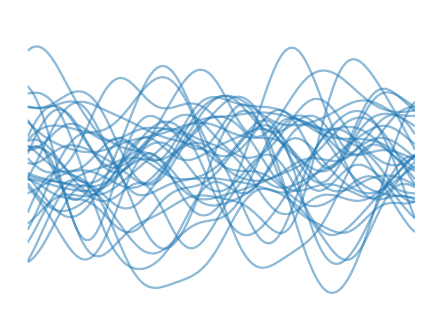
\begin{tikzpicture}
\begin{axis}[axis lines={none}, height={5cm}, width={6.5cm}, xmin={-0.5}, xmax={0.5}, ymin={-1}, ymax={1}]
    \node at (0,-1) {};
    \node at (0,1) {};
    \node at (1,1) {};
    \node at (1,-1) {};
    \addplot[no markers, smooth, thick, color={rgb,1:red,0.1216;green,0.4667;blue,0.7059}, opacity={0.5}]
        coordinates {
            (-0.5,0.15523496138876489)
            (-0.4875,0.1679401303311662)
            (-0.475,0.16611759847147972)
            (-0.4625,0.15047928535692157)
            (-0.45,0.12267475005957877)
            (-0.4375,0.0850542509514219)
            (-0.425,0.04042114810168771)
            (-0.4125,-0.00820008353320275)
            (-0.4,-0.057766463448892816)
            (-0.3875,-0.10538707731732153)
            (-0.375,-0.1484659227732094)
            (-0.3625,-0.18482296655382283)
            (-0.35,-0.21279614837651167)
            (-0.3375,-0.23132102354184564)
            (-0.325,-0.23997866040878257)
            (-0.3125,-0.2389990845571492)
            (-0.3,-0.229208921875162)
            (-0.2875,-0.21191843484446582)
            (-0.275,-0.1887537387129944)
            (-0.2625,-0.16145212207569293)
            (-0.25,-0.1316488385073641)
            (-0.2375,-0.10068936395932451)
            (-0.225,-0.06949979272450844)
            (-0.2125,-0.03853925591782681)
            (-0.2,-0.007843335060488815)
            (-0.1875,0.022850610360514834)
            (-0.175,0.05392251426180429)
            (-0.1625,0.08567177556221282)
            (-0.15,0.11814567768243468)
            (-0.1375,0.15103232390490018)
            (-0.125,0.1836428846188128)
            (-0.1125,0.21498864531205789)
            (-0.1,0.2439373984669441)
            (-0.0875,0.2694158310223021)
            (-0.075,0.2906138250381566)
            (-0.0625,0.30714555564362545)
            (-0.05,0.31913129784384825)
            (-0.0375,0.32718100108705855)
            (-0.025,0.3322821344217253)
            (-0.0125,0.33561520757287205)
            (0.0,0.33833599652288915)
            (0.0125,0.3413703105041543)
            (0.025,0.3452636252431086)
            (0.0375,0.3501149557940032)
            (0.05,0.3556050152234645)
            (0.0625,0.3611075309184579)
            (0.075,0.3658544946232535)
            (0.0875,0.369115267253172)
            (0.1,0.37034825960136886)
            (0.1125,0.36929246425174367)
            (0.125,0.36598218957571643)
            (0.1375,0.36068792122678006)
            (0.15,0.35380447134858206)
            (0.1625,0.3457199889398013)
            (0.175,0.33670296353208473)
            (0.1875,0.3268382216090368)
            (0.2,0.31602866907371036)
            (0.2125,0.30406079935527)
            (0.225,0.2907135678611701)
            (0.2375,0.2758769379060443)
            (0.25,0.25964185440240917)
            (0.2625,0.24232911384391903)
            (0.275,0.22443954851104625)
            (0.2875,0.20652874521601056)
            (0.3,0.18903118436668945)
            (0.3125,0.1720757799093825)
            (0.325,0.15534274764733536)
            (0.3375,0.13800794051166898)
            (0.35,0.11880535827139918)
            (0.3625,0.09621432077369726)
            (0.375,0.06874983853460526)
            (0.3875,0.03530917613081126)
            (0.4,-0.004489636156847693)
            (0.4125,-0.0500462659045535)
            (0.425,-0.09965292162759196)
            (0.4375,-0.15054268318358746)
            (0.45,-0.19911758228810578)
            (0.4625,-0.24132945786921836)
            (0.475,-0.27315774180126634)
            (0.4875,-0.29110973500485193)
            (0.5,-0.29266438066920925)
        }
        ;
    \addplot[no markers, smooth, thick, color={rgb,1:red,0.1216;green,0.4667;blue,0.7059}, opacity={0.5}]
        coordinates {
            (-0.5,-0.006498501542192184)
            (-0.4875,-0.012063128400707626)
            (-0.475,-0.004063372033039539)
            (-0.4625,0.014338696866013967)
            (-0.45,0.03906510497547824)
            (-0.4375,0.0657452310988488)
            (-0.425,0.09034313323334403)
            (-0.4125,0.10968351172383453)
            (-0.4,0.12179054877602216)
            (-0.3875,0.12599055131729)
            (-0.375,0.12277581702447996)
            (-0.3625,0.11347394599251862)
            (-0.35,0.09980416249217747)
            (-0.3375,0.08342218435782292)
            (-0.325,0.06555350904622667)
            (-0.3125,0.04679203811793473)
            (-0.3,0.02710171934952276)
            (-0.2875,0.006011907969518077)
            (-0.275,-0.01704728179046158)
            (-0.2625,-0.04235549851835712)
            (-0.25,-0.06955719538548222)
            (-0.2375,-0.09745047500218505)
            (-0.225,-0.12396960662912146)
            (-0.2125,-0.14637814550950595)
            (-0.2,-0.16164262277211253)
            (-0.1875,-0.1669161589183267)
            (-0.175,-0.1600360111692512)
            (-0.1625,-0.13993450471599608)
            (-0.15,-0.1068799090548913)
            (-0.1375,-0.062498707151288885)
            (-0.125,-0.00957559400446778)
            (-0.1125,0.048327450365678204)
            (-0.1,0.1073563097347679)
            (-0.0875,0.16385917279152443)
            (-0.075,0.21479780899661846)
            (-0.0625,0.25800530696727564)
            (-0.05,0.29225619483928106)
            (-0.0375,0.31715692434445963)
            (-0.025,0.3329030238012235)
            (-0.0125,0.33997538837935376)
            (0.0,0.3388567194261787)
            (0.0125,0.32983871600937176)
            (0.025,0.3129642596812959)
            (0.0375,0.28811306155086636)
            (0.05,0.25520257225771936)
            (0.0625,0.21444688408844367)
            (0.075,0.16660141697944977)
            (0.0875,0.11312351357304715)
            (0.1,0.05619778231876657)
            (0.1125,-0.0013944845755225893)
            (0.125,-0.056547396225835905)
            (0.1375,-0.1061979416528453)
            (0.15,-0.14772148137012459)
            (0.1625,-0.17928145246352226)
            (0.175,-0.20006886124079715)
            (0.1875,-0.21038966725668767)
            (0.2,-0.21158838384135664)
            (0.2125,-0.2058272178785377)
            (0.225,-0.1957651388715092)
            (0.2375,-0.18419544533661236)
            (0.25,-0.1737015308226016)
            (0.2625,-0.16637963223849978)
            (0.275,-0.16365807197747587)
            (0.2875,-0.1662202281135579)
            (0.3,-0.1740187524852652)
            (0.3125,-0.18635579044407166)
            (0.325,-0.20200030009873618)
            (0.3375,-0.21931853671777665)
            (0.35,-0.2364045090206636)
            (0.3625,-0.25120941456304235)
            (0.375,-0.26167821551733256)
            (0.3875,-0.2659042284941533)
            (0.4,-0.2623075757414605)
            (0.4125,-0.2498317919695848)
            (0.425,-0.22813824010884293)
            (0.4375,-0.19776501765316054)
            (0.45,-0.16021050135532577)
            (0.4625,-0.11790499364980878)
            (0.475,-0.07404808540934756)
            (0.4875,-0.032312420120021175)
            (0.5,0.0035580200467923845)
        }
        ;
    \addplot[no markers, smooth, thick, color={rgb,1:red,0.1216;green,0.4667;blue,0.7059}, opacity={0.5}]
        coordinates {
            (-0.5,-0.5961053545429924)
            (-0.4875,-0.5348809289235996)
            (-0.475,-0.4675079696820008)
            (-0.4625,-0.3980791837895431)
            (-0.45,-0.3307786511098768)
            (-0.4375,-0.2694679199759233)
            (-0.425,-0.21733271622403894)
            (-0.4125,-0.1766420558480032)
            (-0.4,-0.14864906920645143)
            (-0.3875,-0.13363572672132903)
            (-0.375,-0.13107744062242496)
            (-0.3625,-0.13988338901142186)
            (-0.35,-0.1586581412087985)
            (-0.3375,-0.18593138734386713)
            (-0.325,-0.22031451283485637)
            (-0.3125,-0.2605624690760413)
            (-0.3,-0.30554245696010846)
            (-0.2875,-0.35413243012169504)
            (-0.275,-0.4050879328152737)
            (-0.2625,-0.45692231103881153)
            (-0.25,-0.5078418317714812)
            (-0.2375,-0.5557647555122117)
            (-0.225,-0.5984347508823558)
            (-0.2125,-0.6336181613742438)
            (-0.2,-0.6593557599529349)
            (-0.1875,-0.6742264168796918)
            (-0.175,-0.6775749719134312)
            (-0.1625,-0.6696603217192245)
            (-0.15,-0.6516914122917801)
            (-0.1375,-0.6257361853638724)
            (-0.125,-0.5945084283093968)
            (-0.1125,-0.5610565532668191)
            (-0.1,-0.5283935939814111)
            (-0.0875,-0.4991170056388717)
            (-0.075,-0.4750691158072615)
            (-0.0625,-0.45708434322393254)
            (-0.05,-0.4448585582978187)
            (-0.0375,-0.43696084978038807)
            (-0.025,-0.4309904783713637)
            (-0.0125,-0.42386400085778225)
            (0.0,-0.41220136531153756)
            (0.0125,-0.3927668844382047)
            (0.025,-0.36291275356522656)
            (0.0375,-0.32097020055554787)
            (0.05,-0.2665370292603545)
            (0.0625,-0.20062032243991557)
            (0.075,-0.12560884073883427)
            (0.0875,-0.045069879630970845)
            (0.1,0.03661206486214663)
            (0.1125,0.11471528502073298)
            (0.125,0.1847213523828721)
            (0.1375,0.24284603951085212)
            (0.15,0.28648791556298453)
            (0.1625,0.3145297907987811)
            (0.175,0.3274465238405866)
            (0.1875,0.32719943872771806)
            (0.2,0.3169290375810418)
            (0.2125,0.30048895220156135)
            (0.225,0.2818898523152747)
            (0.2375,0.26473756237231594)
            (0.25,0.2517516748896788)
            (0.2625,0.2444384750283005)
            (0.275,0.24296660755113683)
            (0.2875,0.24625970298772662)
            (0.3,0.2522830577866085)
            (0.3125,0.2584681515685546)
            (0.325,0.26219552579607047)
            (0.3375,0.2612478657731163)
            (0.35,0.2541528688848072)
            (0.3625,0.24035835730710473)
            (0.375,0.22021583400540898)
            (0.3875,0.19478680265454007)
            (0.4,0.1655212149095328)
            (0.4125,0.13388240869338563)
            (0.425,0.10100280208675191)
            (0.4375,0.0674473135426841)
            (0.45,0.03313832898502986)
            (0.4625,-0.0025384169447078136)
            (0.475,-0.04046654568808898)
            (0.4875,-0.08142525068995565)
            (0.5,-0.12568868907143038)
        }
        ;
    \addplot[no markers, smooth, thick, color={rgb,1:red,0.1216;green,0.4667;blue,0.7059}, opacity={0.5}]
        coordinates {
            (-0.5,0.5102762179520177)
            (-0.4875,0.5166186197708147)
            (-0.475,0.5165087604783452)
            (-0.4625,0.5072103702775616)
            (-0.45,0.48636042561697956)
            (-0.4375,0.4522442147905966)
            (-0.425,0.4039707332621651)
            (-0.4125,0.34154496135812695)
            (-0.4,0.26585002970866384)
            (-0.3875,0.17856133554583142)
            (-0.375,0.08201592942230561)
            (-0.3625,-0.020944244352672267)
            (-0.35,-0.12714412780670886)
            (-0.3375,-0.23325777258365277)
            (-0.325,-0.3359992216392775)
            (-0.3125,-0.43231810433224194)
            (-0.3,-0.5195896932900511)
            (-0.2875,-0.595781274986691)
            (-0.275,-0.6595707157846349)
            (-0.2625,-0.7103924267992759)
            (-0.25,-0.7483926375049695)
            (-0.2375,-0.7742899856879527)
            (-0.225,-0.7891565771677767)
            (-0.2125,-0.7941545659578672)
            (-0.2,-0.7902786898631259)
            (-0.1875,-0.7781611846792555)
            (-0.175,-0.7579889657331753)
            (-0.1625,-0.7295635797841374)
            (-0.15,-0.6925050723202015)
            (-0.1375,-0.6465672984742035)
            (-0.125,-0.5920017578521102)
            (-0.1125,-0.5298872548349433)
            (-0.1,-0.4623393536091265)
            (-0.0875,-0.3925292418487051)
            (-0.075,-0.3244746550728784)
            (-0.0625,-0.26261028366660377)
            (-0.05,-0.21119283171676914)
            (-0.0375,-0.17363653123695916)
            (-0.025,-0.15189917765845568)
            (-0.0125,-0.14604031211942925)
            (0.0,-0.15405018226584816)
            (0.0125,-0.17200382520609342)
            (0.025,-0.19453693571590341)
            (0.0375,-0.21558015379807)
            (0.05,-0.22923798043739244)
            (0.0625,-0.23066807239644269)
            (0.075,-0.21681273227501496)
            (0.0875,-0.18685829665388548)
            (0.1,-0.14234551842715049)
            (0.1125,-0.08691584670453659)
            (0.125,-0.02574271212989513)
            (0.1375,0.035248933514169134)
            (0.15,0.09023782752019491)
            (0.1625,0.134292094487215)
            (0.175,0.1639610297222741)
            (0.1875,0.17759071410846528)
            (0.2,0.17533645804255374)
            (0.2125,0.15890191069659743)
            (0.225,0.1310817303999866)
            (0.2375,0.09521315321763237)
            (0.25,0.05464707611316909)
            (0.2625,0.012331927240861393)
            (0.275,-0.02943108963022746)
            (0.2875,-0.06904615224159058)
            (0.3,-0.10552119435400004)
            (0.3125,-0.13826495625565527)
            (0.325,-0.1668562263638477)
            (0.3375,-0.19085518908774274)
            (0.35,-0.20970683916049207)
            (0.3625,-0.2227560357041954)
            (0.375,-0.22936094992613018)
            (0.3875,-0.22906452699505458)
            (0.4,-0.2217684684722182)
            (0.4125,-0.20785428322616123)
            (0.425,-0.18821048503746146)
            (0.4375,-0.16414987569773318)
            (0.45,-0.13722952111270031)
            (0.4625,-0.10901126953781462)
            (0.475,-0.08081629431521752)
            (0.4875,-0.053529500524193654)
            (0.5,-0.027498374640029716)
        }
        ;
    \addplot[no markers, smooth, thick, color={rgb,1:red,0.1216;green,0.4667;blue,0.7059}, opacity={0.5}]
        coordinates {
            (-0.5,-0.11426081665207924)
            (-0.4875,-0.05400630271062665)
            (-0.475,0.015808762149936595)
            (-0.4625,0.09103067434388502)
            (-0.45,0.16712959182228093)
            (-0.4375,0.2396335219134836)
            (-0.425,0.3045723226120997)
            (-0.4125,0.35886459348356714)
            (-0.4,0.40058782510993396)
            (-0.3875,0.42909104940344006)
            (-0.375,0.4449358820982322)
            (-0.3625,0.44968109271291756)
            (-0.35,0.4455520002573167)
            (-0.3375,0.4350540736519356)
            (-0.325,0.42059679936650196)
            (-0.3125,0.4041881799317961)
            (-0.3,0.38724363764199643)
            (-0.2875,0.37052921970778907)
            (-0.275,0.35423275447711816)
            (-0.2625,0.33813319371292705)
            (-0.25,0.32182221447438963)
            (-0.2375,0.30492602722269796)
            (-0.225,0.28727989626755435)
            (-0.2125,0.2690216146094594)
            (-0.2,0.2505898267331407)
            (-0.1875,0.23263439600835462)
            (-0.175,0.2158646133444161)
            (-0.1625,0.2008733739817854)
            (-0.15,0.18797939667693758)
            (-0.1375,0.1771247924841645)
            (-0.125,0.16785320449002644)
            (-0.1125,0.15937706019679937)
            (-0.1,0.1507246264655887)
            (-0.0875,0.14094193376882702)
            (-0.075,0.12931397435167732)
            (-0.0625,0.11556549064361987)
            (-0.05,0.10000446611343486)
            (-0.0375,0.08358020947715894)
            (-0.025,0.06784088366616409)
            (-0.0125,0.054790208758920336)
            (0.0,0.04665758603186711)
            (0.0125,0.04560812610353708)
            (0.025,0.053427672184284736)
            (0.0375,0.07122218037842201)
            (0.05,0.0991706052958177)
            (0.0625,0.13636600520409992)
            (0.075,0.18077144606566753)
            (0.0875,0.22930611646738314)
            (0.1,0.27806365522647314)
            (0.1125,0.322649993389412)
            (0.125,0.3586132105915459)
            (0.1375,0.38192446737760505)
            (0.15,0.3894586969031012)
            (0.1625,0.37941818347757195)
            (0.175,0.35164296436703596)
            (0.1875,0.3077601316027492)
            (0.2,0.25113962385223665)
            (0.2125,0.18664585815992563)
            (0.225,0.12020021330377477)
            (0.2375,0.0581955771393931)
            (0.25,0.006826974653830975)
            (0.2625,-0.028582166745060644)
            (0.275,-0.04417336779664334)
            (0.2875,-0.03798812566278942)
            (0.3,-0.01018526201831469)
            (0.3125,0.03699064027817118)
            (0.325,0.09948723836658137)
            (0.3375,0.17193221837558664)
            (0.35,0.24826496253969405)
            (0.3625,0.3224265626447975)
            (0.375,0.38901585676269623)
            (0.3875,0.44382627526093865)
            (0.4,0.4841980264778301)
            (0.4125,0.5091491563113336)
            (0.425,0.5192824087514898)
            (0.4375,0.5164971200639391)
            (0.45,0.5035615025809779)
            (0.4625,0.4836167896952628)
            (0.475,0.45968888818206893)
            (0.4875,0.43427561638339746)
            (0.5,0.40906045673967506)
        }
        ;
    \addplot[no markers, smooth, thick, color={rgb,1:red,0.1216;green,0.4667;blue,0.7059}, opacity={0.5}]
        coordinates {
            (-0.5,-0.37509266484803305)
            (-0.4875,-0.2905600531205952)
            (-0.475,-0.21721127510245922)
            (-0.4625,-0.15841590729979868)
            (-0.45,-0.115614410272327)
            (-0.4375,-0.08820153605692937)
            (-0.425,-0.07367886170178811)
            (-0.4125,-0.06806808223782457)
            (-0.4,-0.06653765619018764)
            (-0.3875,-0.06415903651867988)
            (-0.375,-0.056682083918497855)
            (-0.3625,-0.041208664914520826)
            (-0.35,-0.016652897184496265)
            (-0.3375,0.016093532675440468)
            (-0.325,0.054325788971458316)
            (-0.3125,0.09399882132148905)
            (-0.3,0.13043241952094192)
            (-0.2875,0.15912846090088906)
            (-0.275,0.1765576770944545)
            (-0.2625,0.18077675438373128)
            (-0.25,0.1717666342006028)
            (-0.2375,0.15143436387644915)
            (-0.225,0.12328399627208048)
            (-0.2125,0.09182435168087108)
            (-0.2,0.06183029026480996)
            (-0.1875,0.03759942191300668)
            (-0.175,0.02234263756760571)
            (-0.1625,0.01781527170138532)
            (-0.15,0.024242880599628668)
            (-0.1375,0.04053292262340544)
            (-0.125,0.06470458509361984)
            (-0.1125,0.09442633770452637)
            (-0.1,0.12753358931733483)
            (-0.0875,0.16241049012770023)
            (-0.075,0.19815739652417505)
            (-0.0625,0.234519946603302)
            (-0.05,0.27161441719072127)
            (-0.0375,0.30953344840002056)
            (-0.025,0.3479448994954918)
            (-0.0125,0.38579791314428824)
            (0.0,0.4212239380205375)
            (0.0125,0.4516726633011426)
            (0.025,0.47426477868620254)
            (0.0375,0.48628889616480936)
            (0.05,0.4857318679696318)
            (0.0625,0.47171938643993083)
            (0.075,0.44476049143956736)
            (0.0875,0.40673198478254113)
            (0.1,0.36059723476352795)
            (0.1125,0.3099149956051932)
            (0.125,0.2582433689052451)
            (0.1375,0.208570072888895)
            (0.15,0.16289619983226122)
            (0.1625,0.12206694371459771)
            (0.175,0.08588659205768245)
            (0.1875,0.05348897517950976)
            (0.2,0.023873667925105563)
            (0.2125,-0.0035232449001952187)
            (0.225,-0.028367072558917187)
            (0.2375,-0.049193460800960764)
            (0.25,-0.06348095727612747)
            (0.2625,-0.06803173763836745)
            (0.275,-0.05959372946650533)
            (0.2875,-0.03559884267859403)
            (0.3,0.005140302001665771)
            (0.3125,0.06193106603311564)
            (0.325,0.13201879795218724)
            (0.3375,0.21077895388085457)
            (0.35,0.29226334235744833)
            (0.3625,0.3700065007041237)
            (0.375,0.4379430252169951)
            (0.3875,0.4912623175668449)
            (0.4,0.5270390183405674)
            (0.4125,0.5445228801050208)
            (0.425,0.5450412137252638)
            (0.4375,0.5315454384642463)
            (0.45,0.5079039640351156)
            (0.4625,0.47809174723353853)
            (0.475,0.4454425682748759)
            (0.4875,0.4121106666141692)
            (0.5,0.3788387823802266)
        }
        ;
    \addplot[no markers, smooth, thick, color={rgb,1:red,0.1216;green,0.4667;blue,0.7059}, opacity={0.5}]
        coordinates {
            (-0.5,-0.09661325684452346)
            (-0.4875,-0.1098397334293191)
            (-0.475,-0.12119067830061706)
            (-0.4625,-0.12997971427253568)
            (-0.45,-0.13620800390312945)
            (-0.4375,-0.1406344349582525)
            (-0.425,-0.14466033233582679)
            (-0.4125,-0.15004255135935757)
            (-0.4,-0.15848813244214774)
            (-0.3875,-0.17121345680984065)
            (-0.375,-0.18856427918424093)
            (-0.3625,-0.20978658485298754)
            (-0.35,-0.23301242985861775)
            (-0.3375,-0.2554843242639795)
            (-0.325,-0.2739940635054955)
            (-0.3125,-0.2854666392006094)
            (-0.3,-0.28758619746860103)
            (-0.2875,-0.2793461030859008)
            (-0.275,-0.2614125919082063)
            (-0.2625,-0.23622049691738561)
            (-0.25,-0.20776511730604813)
            (-0.2375,-0.18110816567604693)
            (-0.225,-0.16166787359691603)
            (-0.2125,-0.15440399111481334)
            (-0.2,-0.16302992853577136)
            (-0.1875,-0.18938258182258366)
            (-0.175,-0.23305570656784524)
            (-0.1625,-0.29135954519158314)
            (-0.15,-0.3596155859949783)
            (-0.1375,-0.4317404733483052)
            (-0.125,-0.5010268173654502)
            (-0.1125,-0.5609988101965757)
            (-0.1,-0.6062118280917791)
            (-0.0875,-0.6328783729744065)
            (-0.075,-0.639234696706449)
            (-0.0625,-0.625607022999211)
            (-0.05,-0.5941853308911668)
            (-0.0375,-0.5485577549753919)
            (-0.025,-0.4930925346353133)
            (-0.0125,-0.43227222435421525)
            (0.0,-0.3700847326155304)
            (0.0125,-0.3095590008728406)
            (0.025,-0.2525037391569958)
            (0.0375,-0.19947132745085305)
            (0.05,-0.1499321258651602)
            (0.0625,-0.10261287296866742)
            (0.075,-0.055931044449640345)
            (0.0875,-0.008447470657554912)
            (0.1,0.04073749801770888)
            (0.1125,0.09170504513830352)
            (0.125,0.14359509375733173)
            (0.1375,0.19465273804839917)
            (0.15,0.24243110335058857)
            (0.1625,0.28411552078667435)
            (0.175,0.3169178610248618)
            (0.1875,0.3384817444479126)
            (0.2,0.3472396404492053)
            (0.2125,0.34267104680516103)
            (0.225,0.3254255831621693)
            (0.2375,0.2972938624796748)
            (0.25,0.26102992190060637)
            (0.2625,0.22004913202139703)
            (0.275,0.17804228742596404)
            (0.2875,0.13855780657148545)
            (0.3,0.1046080708958155)
            (0.3125,0.07835222778164944)
            (0.325,0.060896633889119534)
            (0.3375,0.052236979515740856)
            (0.35,0.05134543778616488)
            (0.3625,0.05638502575047237)
            (0.375,0.06501507011333188)
            (0.3875,0.07473923370532383)
            (0.4,0.08324310037889947)
            (0.4125,0.08867264342780687)
            (0.425,0.08981728545263645)
            (0.4375,0.08617948323855035)
            (0.45,0.07793349715029188)
            (0.4625,0.06579535847717312)
            (0.475,0.05084036914494971)
            (0.4875,0.03431104239456659)
            (0.5,0.017456027899036684)
        }
        ;
    \addplot[no markers, smooth, thick, color={rgb,1:red,0.1216;green,0.4667;blue,0.7059}, opacity={0.5}]
        coordinates {
            (-0.5,0.09049918356815218)
            (-0.4875,0.09349129164263725)
            (-0.475,0.10803646896177127)
            (-0.4625,0.13276918520190997)
            (-0.45,0.16476480750528244)
            (-0.4375,0.19992544301526952)
            (-0.425,0.23359952311043727)
            (-0.4125,0.2613253986300846)
            (-0.4,0.2795615647314192)
            (-0.3875,0.2862659642945627)
            (-0.375,0.28121459020784945)
            (-0.3625,0.26599983087849555)
            (-0.35,0.24371137324678607)
            (-0.3375,0.21836406605424086)
            (-0.325,0.19418518899802428)
            (-0.3125,0.17489822565887286)
            (-0.3,0.16313669056967656)
            (-0.2875,0.160091048660282)
            (-0.275,0.1654412465859728)
            (-0.2625,0.17756795604589126)
            (-0.25,0.19398009134409433)
            (-0.2375,0.21185615340338476)
            (-0.225,0.2285804565761982)
            (-0.2125,0.24216496317055153)
            (-0.2,0.25148013316097334)
            (-0.1875,0.25626577627168534)
            (-0.175,0.25694421427008135)
            (-0.1625,0.25430149613820896)
            (-0.15,0.24912848158202003)
            (-0.1375,0.2419170734108832)
            (-0.125,0.2326877989964773)
            (-0.1125,0.22098853445775002)
            (-0.1,0.20605948628343537)
            (-0.0875,0.18711731353153072)
            (-0.075,0.16368137209113057)
            (-0.0625,0.1358542790751358)
            (-0.05,0.10447952665497387)
            (-0.0375,0.07112791621980835)
            (-0.025,0.03790508297526181)
            (-0.0125,0.007114753800624538)
            (0.0,-0.019153223155249022)
            (0.0125,-0.039422458191513375)
            (0.025,-0.05313088598233434)
            (0.0375,-0.06076719785770183)
            (0.05,-0.06381206867282044)
            (0.0625,-0.06449458942758676)
            (0.075,-0.06541242002593214)
            (0.0875,-0.0690908517690299)
            (0.1,-0.07756572122646427)
            (0.1125,-0.09206647407345689)
            (0.125,-0.11285138893068475)
            (0.1375,-0.1392132155156996)
            (0.15,-0.16963829639551556)
            (0.1625,-0.20207357285766872)
            (0.175,-0.23423971607171365)
            (0.1875,-0.26392768828724456)
            (0.2,-0.2892292665800138)
            (0.2125,-0.3086750586476655)
            (0.225,-0.3212798066210653)
            (0.2375,-0.32651741001331613)
            (0.25,-0.3242615457343479)
            (0.2625,-0.3147291617372696)
            (0.275,-0.2984539433830001)
            (0.2875,-0.27629867382815876)
            (0.3,-0.2494948931897748)
            (0.3125,-0.21968161419498444)
            (0.325,-0.18890716635216015)
            (0.3375,-0.15956212943258297)
            (0.35,-0.13422619995667215)
            (0.3625,-0.11543405427185977)
            (0.375,-0.10538901533927383)
            (0.3875,-0.10567212295971856)
            (0.4,-0.11700260582760087)
            (0.4125,-0.13910080763005922)
            (0.425,-0.1706867221996772)
            (0.4375,-0.20962019932093875)
            (0.45,-0.2531588679548634)
            (0.4625,-0.29828417668112406)
            (0.475,-0.3420311690290604)
            (0.4875,-0.3817577355852279)
            (0.5,-0.41530460077889514)
        }
        ;
    \addplot[no markers, smooth, thick, color={rgb,1:red,0.1216;green,0.4667;blue,0.7059}, opacity={0.5}]
        coordinates {
            (-0.5,-0.12669243465158064)
            (-0.4875,-0.1377801930587315)
            (-0.475,-0.1562694143670687)
            (-0.4625,-0.1793092525432064)
            (-0.45,-0.20363022598416142)
            (-0.4375,-0.22613794022484754)
            (-0.425,-0.2444726077414054)
            (-0.4125,-0.2574333856203718)
            (-0.4,-0.2651879427047159)
            (-0.3875,-0.26922454362934156)
            (-0.375,-0.27205004286558393)
            (-0.3625,-0.27668419443420017)
            (-0.35,-0.28603974800459964)
            (-0.3375,-0.3023012549574903)
            (-0.325,-0.32641843242270063)
            (-0.3125,-0.3578112298771307)
            (-0.3,-0.39434646682977925)
            (-0.2875,-0.43259678294136017)
            (-0.275,-0.4683408108676936)
            (-0.2625,-0.49721876145821453)
            (-0.25,-0.5154285540188938)
            (-0.2375,-0.5203398187973326)
            (-0.225,-0.5109180387555634)
            (-0.2125,-0.4878858716099411)
            (-0.2,-0.45359655943437505)
            (-0.1875,-0.41164606957495453)
            (-0.175,-0.36629636186848386)
            (-0.1625,-0.3218134192194526)
            (-0.15,-0.2818348941953498)
            (-0.1375,-0.24887194478181573)
            (-0.125,-0.2240208368614876)
            (-0.1125,-0.2069185323559006)
            (-0.1,-0.19593129514514954)
            (-0.0875,-0.18852524286856703)
            (-0.075,-0.18174020756465292)
            (-0.0625,-0.17267777326074102)
            (-0.05,-0.1589217349432253)
            (-0.0375,-0.13883155235795566)
            (-0.025,-0.11168081809769244)
            (-0.0125,-0.07764596536748523)
            (0.0,-0.03767819632915945)
            (0.0125,0.006691579513840695)
            (0.025,0.05356180377095792)
            (0.0375,0.10084010444724911)
            (0.05,0.1463698319245763)
            (0.0625,0.18800212215796896)
            (0.075,0.22363275395010052)
            (0.0875,0.25123570863789274)
            (0.1,0.26892697831797696)
            (0.1125,0.2750824510827422)
            (0.125,0.2685151703890038)
            (0.1375,0.24869471849026165)
            (0.15,0.2159708064368794)
            (0.1625,0.17174995246909341)
            (0.175,0.11857234575865828)
            (0.1875,0.06004698527491478)
            (0.2,0.0006253722682283969)
            (0.2125,-0.05477679363589122)
            (0.225,-0.10127024917604018)
            (0.2375,-0.13453058053035719)
            (0.25,-0.15130572355227725)
            (0.2625,-0.1498137609945364)
            (0.275,-0.1299666220885393)
            (0.2875,-0.09338170395657495)
            (0.3,-0.04317698947221349)
            (0.3125,0.016420321103092352)
            (0.325,0.08059265604099715)
            (0.3375,0.14450099844259096)
            (0.35,0.20382168733460668)
            (0.3625,0.2551779597429412)
            (0.375,0.29641373988998826)
            (0.3875,0.32668505858718)
            (0.4,0.34637421665959944)
            (0.4125,0.35685807344308523)
            (0.425,0.3601804172209532)
            (0.4375,0.3586868429117924)
            (0.45,0.35467861146758106)
            (0.4625,0.35013122453723905)
            (0.475,0.34650694553579503)
            (0.4875,0.34467189461773673)
            (0.5,0.3449111284507212)
        }
        ;
    \addplot[no markers, smooth, thick, color={rgb,1:red,0.1216;green,0.4667;blue,0.7059}, opacity={0.5}]
        coordinates {
            (-0.5,0.06367056415047723)
            (-0.4875,0.14482945053534013)
            (-0.475,0.21999084434041524)
            (-0.4625,0.28530639312804834)
            (-0.45,0.3373258251578678)
            (-0.4375,0.3732855231035389)
            (-0.425,0.3913614182000512)
            (-0.4125,0.39086122673446677)
            (-0.4,0.37233287153943134)
            (-0.3875,0.3375708889908817)
            (-0.375,0.28951105305012237)
            (-0.3625,0.23201499046612212)
            (-0.35,0.16956004222825136)
            (-0.3375,0.10686314180734627)
            (-0.325,0.04847868028916624)
            (-0.3125,-0.0015831386286056376)
            (-0.3,-0.04017091596921569)
            (-0.2875,-0.0652004061416823)
            (-0.275,-0.07573150179401876)
            (-0.2625,-0.07190788919200852)
            (-0.25,-0.05477450078192805)
            (-0.2375,-0.026007270419920687)
            (-0.225,0.012396283068345875)
            (-0.2125,0.058411331296434325)
            (-0.2,0.110214471647349)
            (-0.1875,0.1663098091378385)
            (-0.175,0.22553576099293424)
            (-0.1625,0.28695997887919)
            (-0.15,0.3496928098249642)
            (-0.1375,0.41266724535072863)
            (-0.125,0.47444174961758606)
            (-0.1125,0.5330797845208259)
            (-0.1,0.5861464350435214)
            (-0.0875,0.6308405799952094)
            (-0.075,0.6642545746019796)
            (-0.0625,0.6837274044805366)
            (-0.05,0.6872367328993202)
            (-0.0375,0.6737642191955057)
            (-0.025,0.6435691916093662)
            (-0.0125,0.5983182507842891)
            (0.0,0.5410404701399587)
            (0.0125,0.47590555598596457)
            (0.025,0.4078506248032511)
            (0.0375,0.3421050932850786)
            (0.05,0.2836784256202669)
            (0.0625,0.23687969717712107)
            (0.075,0.2049307733006195)
            (0.0875,0.18971812011442588)
            (0.1,0.19170528872723536)
            (0.1125,0.2100033132626637)
            (0.125,0.24257405915880953)
            (0.1375,0.28652557546048757)
            (0.15,0.3384509227359072)
            (0.1625,0.3947631830620504)
            (0.175,0.45198812172479463)
            (0.1875,0.5069896700514385)
            (0.2,0.5571187800817881)
            (0.2125,0.6002900748433408)
            (0.225,0.6350006143113033)
            (0.2375,0.6603097163549877)
            (0.25,0.6757981369850999)
            (0.2625,0.68152022073286)
            (0.275,0.6779558479095156)
            (0.2875,0.6659623283522708)
            (0.3,0.6467216980323759)
            (0.3125,0.6216772924102921)
            (0.325,0.5924551595524913)
            (0.3375,0.5607700678002467)
            (0.35,0.5283211230576793)
            (0.3625,0.49668665696679487)
            (0.375,0.4672306076353314)
            (0.3875,0.4410322149545603)
            (0.4,0.41884743699018917)
            (0.4125,0.401104830223073)
            (0.425,0.3879321103027188)
            (0.4375,0.37920386431118214)
            (0.45,0.37459739678132775)
            (0.4625,0.37364338977826295)
            (0.475,0.3757610823734664)
            (0.4875,0.380273329877988)
            (0.5,0.38640381357539344)
        }
        ;
    \addplot[no markers, smooth, thick, color={rgb,1:red,0.1216;green,0.4667;blue,0.7059}, opacity={0.5}]
        coordinates {
            (-0.5,0.18923845665592104)
            (-0.4875,0.2616049879659079)
            (-0.475,0.32315996045490125)
            (-0.4625,0.37099932247593653)
            (-0.45,0.4030200323989503)
            (-0.4375,0.4180831265806481)
            (-0.425,0.41609040139802944)
            (-0.4125,0.3979748268999415)
            (-0.4,0.36561331990318074)
            (-0.3875,0.3216762308218778)
            (-0.375,0.2694305979702626)
            (-0.3625,0.21251432060702374)
            (-0.35,0.15469679209367015)
            (-0.3375,0.09963928954342453)
            (-0.325,0.0506664780146165)
            (-0.3125,0.010559318488693785)
            (-0.3,-0.0186204756224285)
            (-0.2875,-0.035663943830726574)
            (-0.275,-0.040295790401929724)
            (-0.2625,-0.033193211934373856)
            (-0.25,-0.01593600132645586)
            (-0.2375,0.009113843964461172)
            (-0.225,0.038998220498441115)
            (-0.2125,0.07040253606598765)
            (-0.2,0.09992964814579192)
            (-0.1875,0.12438364317064562)
            (-0.175,0.14103655472741145)
            (-0.1625,0.14785221805364845)
            (-0.15,0.1436460854328389)
            (-0.1375,0.12816730808576404)
            (-0.125,0.1020984953626176)
            (-0.1125,0.06697776216124872)
            (-0.1,0.02505546800612848)
            (-0.0875,-0.020896718241443523)
            (-0.075,-0.06780469130934333)
            (-0.0625,-0.11251988357271066)
            (-0.05,-0.15204065281388848)
            (-0.0375,-0.1837156210765135)
            (-0.025,-0.20542151994620506)
            (-0.0125,-0.21571085010721522)
            (0.0,-0.21392559163627484)
            (0.0125,-0.20027239672461292)
            (0.025,-0.17585287986665232)
            (0.0375,-0.1426409592233105)
            (0.05,-0.10339899770057395)
            (0.0625,-0.06152681150166005)
            (0.075,-0.020842961069593074)
            (0.0875,0.014694160770712162)
            (0.1,0.04130816695735126)
            (0.1125,0.05574248704905786)
            (0.125,0.05557967468097606)
            (0.1375,0.03950432286019167)
            (0.15,0.007473786078759984)
            (0.1625,-0.039231040598285735)
            (0.175,-0.09808927463132032)
            (0.1875,-0.16555538738292702)
            (0.2,-0.23738584359341408)
            (0.2125,-0.30904052698968837)
            (0.225,-0.3761111177373577)
            (0.2375,-0.4347240454416727)
            (0.25,-0.4818688525392576)
            (0.2625,-0.5156134207638213)
            (0.275,-0.5351839085890978)
            (0.2875,-0.5409067870031372)
            (0.3,-0.534029875920976)
            (0.3125,-0.5164556361775235)
            (0.325,-0.49043061076152916)
            (0.3375,-0.4582383070041808)
            (0.35,-0.4219387083894652)
            (0.3625,-0.38318701074474015)
            (0.375,-0.34314914817694764)
            (0.3875,-0.3025149056247479)
            (0.4,-0.26159374524086837)
            (0.4125,-0.22046638510191813)
            (0.425,-0.17915838334180248)
            (0.4375,-0.13780121898302408)
            (0.45,-0.09675129241218274)
            (0.4625,-0.05664665260812614)
            (0.475,-0.01839322875997175)
            (0.4875,0.0169152233026593)
            (0.5,0.04812836187632947)
        }
        ;
    \addplot[no markers, smooth, thick, color={rgb,1:red,0.1216;green,0.4667;blue,0.7059}, opacity={0.5}]
        coordinates {
            (-0.5,-0.7345169701411117)
            (-0.4875,-0.6679815450601592)
            (-0.475,-0.5931706661924058)
            (-0.4625,-0.5142156342812185)
            (-0.45,-0.43529827944952143)
            (-0.4375,-0.36025355905835504)
            (-0.425,-0.29220815336842254)
            (-0.4125,-0.2333105156742481)
            (-0.4,-0.1845938783530289)
            (-0.3875,-0.1459912298317081)
            (-0.375,-0.11649461774766619)
            (-0.3625,-0.09442567725521894)
            (-0.35,-0.07776527799877758)
            (-0.3375,-0.06448159925366712)
            (-0.325,-0.05279958297120861)
            (-0.3125,-0.041369784997163844)
            (-0.3,-0.02931789206167061)
            (-0.2875,-0.016182566308275338)
            (-0.275,-0.0017730990898582894)
            (-0.2625,0.014005559157623065)
            (-0.25,0.0313079355576977)
            (-0.2375,0.0504381688965814)
            (-0.225,0.0718477179080227)
            (-0.2125,0.09603736545905431)
            (-0.2,0.12338528192848693)
            (-0.1875,0.15394312219459894)
            (-0.175,0.1872528375603983)
            (-0.1625,0.22223551615180204)
            (-0.15,0.25719024194698575)
            (-0.1375,0.28991848152172506)
            (-0.125,0.3179627370841335)
            (-0.1125,0.33892301063034314)
            (-0.1,0.35079657274319076)
            (-0.0875,0.3522796505039651)
            (-0.075,0.3429755398384823)
            (-0.0625,0.32347111673920625)
            (-0.05,0.2952690502081041)
            (-0.0375,0.26059078340296293)
            (-0.025,0.22208961799629104)
            (-0.0125,0.18252888100528822)
            (0.0,0.14448397011978703)
            (0.0125,0.11011847796371702)
            (0.025,0.081065728967224)
            (0.0375,0.05842229401590046)
            (0.05,0.04283498629640767)
            (0.0625,0.034643077319480825)
            (0.075,0.034027334225066014)
            (0.0875,0.041119083244166466)
            (0.1,0.05603529798207654)
            (0.1125,0.07882662120350284)
            (0.125,0.10934936369880979)
            (0.1375,0.14709427817501067)
            (0.15,0.19101921451601345)
            (0.1625,0.23943622531835818)
            (0.175,0.28999532255661464)
            (0.1875,0.33978853000206366)
            (0.2,0.3855730351568282)
            (0.2125,0.42408642641416805)
            (0.225,0.4524057624926163)
            (0.2375,0.468290170857874)
            (0.25,0.47044649236507424)
            (0.2625,0.45866938337845403)
            (0.275,0.43382895924042264)
            (0.2875,0.3977062315548912)
            (0.3,0.35270390169423155)
            (0.3125,0.30148221369125255)
            (0.325,0.2465823496332958)
            (0.3375,0.19010100665274135)
            (0.35,0.13346937725090244)
            (0.3625,0.0773700281660838)
            (0.375,0.021800073329090994)
            (0.3875,-0.033736675987700415)
            (0.4,-0.08994760215991848)
            (0.4125,-0.14743230496185947)
            (0.425,-0.2063842921998711)
            (0.4375,-0.26636553765779014)
            (0.45,-0.32619256900036536)
            (0.4625,-0.38395383923563164)
            (0.475,-0.4371573015637859)
            (0.4875,-0.48298772621661457)
            (0.5,-0.518638102814898)
        }
        ;
    \addplot[no markers, smooth, thick, color={rgb,1:red,0.1216;green,0.4667;blue,0.7059}, opacity={0.5}]
        coordinates {
            (-0.5,-0.23130972368072916)
            (-0.4875,-0.21368469374704066)
            (-0.475,-0.19446185007166986)
            (-0.4625,-0.17406508141490062)
            (-0.45,-0.15316673600384847)
            (-0.4375,-0.13258394095009607)
            (-0.425,-0.11317939679797315)
            (-0.4125,-0.09578477136150143)
            (-0.4,-0.08115388309498026)
            (-0.3875,-0.06994143183050823)
            (-0.375,-0.06269435772384302)
            (-0.3625,-0.05983937889860089)
            (-0.35,-0.06165279967421372)
            (-0.3375,-0.06820652707487393)
            (-0.325,-0.07929512853875456)
            (-0.3125,-0.09435954988700651)
            (-0.3,-0.11243054662834112)
            (-0.2875,-0.13211648694117284)
            (-0.275,-0.15165492224338742)
            (-0.2625,-0.16903591200315696)
            (-0.25,-0.18218990136094027)
            (-0.2375,-0.1892174702731032)
            (-0.225,-0.1886262849172564)
            (-0.2125,-0.17953524403193516)
            (-0.2,-0.16180885711827492)
            (-0.1875,-0.1360961440457833)
            (-0.175,-0.10376568861093244)
            (-0.1625,-0.0667482760845837)
            (-0.15,-0.02731644316282808)
            (-0.1375,0.012157808787517911)
            (-0.125,0.04942278051048119)
            (-0.1125,0.082506582489582)
            (-0.1,0.10979368937576822)
            (-0.0875,0.13001605625057638)
            (-0.075,0.1421771465773825)
            (-0.0625,0.14544387250033275)
            (-0.05,0.139049922834639)
            (-0.0375,0.12225200692507347)
            (-0.025,0.09436822898244054)
            (-0.0125,0.054907533454069166)
            (0.0,0.003775208612564765)
            (0.0125,-0.058482941726818574)
            (0.025,-0.1304508519913233)
            (0.0375,-0.20968517324730707)
            (0.05,-0.2926822856749738)
            (0.0625,-0.375002304478437)
            (0.075,-0.45155655992993243)
            (0.0875,-0.5170354095101242)
            (0.1,-0.5664261947677661)
            (0.1125,-0.5955519782579283)
            (0.125,-0.6015541754127042)
            (0.1375,-0.5832478689490828)
            (0.15,-0.5412964660308648)
            (0.1625,-0.4781791496645361)
            (0.175,-0.39795541404109475)
            (0.1875,-0.305860390106676)
            (0.2,-0.20778767053534403)
            (0.2125,-0.10972934633558286)
            (0.225,-0.017244391534129357)
            (0.2375,0.06498302593009116)
            (0.25,0.1334517706235861)
            (0.2625,0.1859977167352755)
            (0.275,0.2217959218124034)
            (0.2875,0.24123331966881503)
            (0.3,0.24568799893082258)
            (0.3125,0.2372574174982948)
            (0.325,0.2184768992292453)
            (0.3375,0.1920628810404687)
            (0.35,0.1607048088253765)
            (0.3625,0.1269177160605844)
            (0.375,0.09295646997254356)
            (0.3875,0.06078391765048964)
            (0.4,0.0320794288914626)
            (0.4125,0.008271646083171734)
            (0.425,-0.009420824795002624)
            (0.4375,-0.019955152077774835)
            (0.45,-0.022447550276865822)
            (0.4625,-0.016180996010517826)
            (0.475,-0.0006394505970335074)
            (0.4875,0.024434621406582376)
            (0.5,0.058968012151304976)
        }
        ;
    \addplot[no markers, smooth, thick, color={rgb,1:red,0.1216;green,0.4667;blue,0.7059}, opacity={0.5}]
        coordinates {
            (-0.5,-0.5012322920696959)
            (-0.4875,-0.4322019198216696)
            (-0.475,-0.35509343480507055)
            (-0.4625,-0.27260501542135174)
            (-0.45,-0.18798513974262906)
            (-0.4375,-0.10473738800538779)
            (-0.425,-0.026303658210233866)
            (-0.4125,0.04423236045818052)
            (-0.4,0.10438823289159821)
            (-0.3875,0.15245157440583318)
            (-0.375,0.18756692752540097)
            (-0.3625,0.2097440072269496)
            (-0.35,0.2197976947852842)
            (-0.3375,0.21923301950416516)
            (-0.325,0.21008791193835993)
            (-0.3125,0.19474451857686775)
            (-0.3,0.17571832626233683)
            (-0.2875,0.15543477667905004)
            (-0.275,0.13600598554382248)
            (-0.2625,0.11902493245259885)
            (-0.25,0.10539930852794271)
            (-0.2375,0.09524978243141394)
            (-0.225,0.08789558809479503)
            (-0.2125,0.0819427327604333)
            (-0.2,0.07547687453640875)
            (-0.1875,0.06634575840215037)
            (-0.175,0.05249817676057337)
            (-0.1625,0.03233167719128538)
            (-0.15,0.004993514225604234)
            (-0.1375,-0.029418599035497248)
            (-0.125,-0.06979664331484026)
            (-0.1125,-0.11412202758803089)
            (-0.1,-0.15971587257642372)
            (-0.0875,-0.20360260597164698)
            (-0.075,-0.24292668796692468)
            (-0.0625,-0.27534968437018875)
            (-0.05,-0.2993558933403589)
            (-0.0375,-0.31440989709334843)
            (-0.025,-0.32093639509367333)
            (-0.0125,-0.32012653104676203)
            (0.0,-0.3136090442368477)
            (0.0125,-0.3030520229335335)
            (0.025,-0.2897760100694554)
            (0.0375,-0.27445829754178896)
            (0.05,-0.2569912143854701)
            (0.0625,-0.23652714729755497)
            (0.075,-0.2117057551720835)
            (0.0875,-0.18102176189149283)
            (0.1,-0.1432623141677456)
            (0.1125,-0.09792717872192144)
            (0.125,-0.045546303587015446)
            (0.1375,0.012172655302446447)
            (0.15,0.0724028684019004)
            (0.1625,0.131460478082301)
            (0.175,0.1852299043933107)
            (0.1875,0.22968173916107154)
            (0.2,0.26139614759210855)
            (0.2125,0.2780047227318177)
            (0.225,0.2784798815745201)
            (0.2375,0.26322956298697026)
            (0.25,0.2339902461950213)
            (0.2625,0.1935461442827405)
            (0.275,0.1453302210653638)
            (0.2875,0.0929785299789594)
            (0.3,0.03991101137480754)
            (0.3125,-0.0109999984140427)
            (0.325,-0.057634350002514045)
            (0.3375,-0.09868963580032844)
            (0.35,-0.13362190937405466)
            (0.3625,-0.16249614719166097)
            (0.375,-0.1857919823141704)
            (0.3875,-0.20421052825893435)
            (0.4,-0.21851887205686465)
            (0.4125,-0.22945311732384027)
            (0.425,-0.23768288007519991)
            (0.4375,-0.2438241623219286)
            (0.45,-0.24847697464305782)
            (0.4625,-0.25226081996025373)
            (0.475,-0.2558252115293641)
            (0.4875,-0.25982210493400587)
            (0.5,-0.2648396287325691)
        }
        ;
    \addplot[no markers, smooth, thick, color={rgb,1:red,0.1216;green,0.4667;blue,0.7059}, opacity={0.5}]
        coordinates {
            (-0.5,-0.10899644267860609)
            (-0.4875,-0.14785443725581482)
            (-0.475,-0.19153046865129736)
            (-0.4625,-0.23755590586989933)
            (-0.45,-0.2830479759544361)
            (-0.4375,-0.3249877051588083)
            (-0.425,-0.3605062518732836)
            (-0.4125,-0.3871400181259711)
            (-0.4,-0.4030201314277851)
            (-0.3875,-0.40697293357945274)
            (-0.375,-0.3985232600743632)
            (-0.3625,-0.3778089892752977)
            (-0.35,-0.34543063537505997)
            (-0.3375,-0.3022708280775051)
            (-0.325,-0.24932319226574787)
            (-0.3125,-0.187567330853384)
            (-0.3,-0.11791659221523107)
            (-0.2875,-0.041249709422194705)
            (-0.275,0.041480995830737354)
            (-0.2625,0.12908990714261281)
            (-0.25,0.21998559663339995)
            (-0.2375,0.3120308160275762)
            (-0.225,0.4024782550345698)
            (-0.2125,0.4880144688165562)
            (-0.2,0.5649262796616665)
            (-0.1875,0.6293816391639206)
            (-0.175,0.677794367812935)
            (-0.1625,0.7072235877205586)
            (-0.15,0.7157477119984749)
            (-0.1375,0.7027519780053244)
            (-0.125,0.6690783782689831)
            (-0.1125,0.6170061673603313)
            (-0.1,0.5500568383352596)
            (-0.0875,0.4726452307886306)
            (-0.075,0.38962341095911107)
            (-0.0625,0.30578168528195865)
            (-0.05,0.22537831283740326)
            (-0.0375,0.1517647421878337)
            (-0.025,0.08715721360956115)
            (-0.0125,0.032581067223767246)
            (0.0,-0.012014638168843406)
            (0.0125,-0.047502499368394555)
            (0.025,-0.07523460045023737)
            (0.0375,-0.0966778004669041)
            (0.05,-0.11309226077310391)
            (0.0625,-0.12530804929978)
            (0.075,-0.13363413038574687)
            (0.0875,-0.13790781111863393)
            (0.1,-0.13766564319215788)
            (0.1125,-0.13239384472086166)
            (0.125,-0.12180166360643316)
            (0.1375,-0.10605733611913723)
            (0.15,-0.08593395873731044)
            (0.1625,-0.06283014462259484)
            (0.175,-0.038654447150594615)
            (0.1875,-0.015588718511228474)
            (0.2,0.004230968170365272)
            (0.2125,0.019060709235049364)
            (0.225,0.027860743141914737)
            (0.2375,0.030515667480176402)
            (0.25,0.027920089488394598)
            (0.2625,0.021908923903336076)
            (0.275,0.01503717637693714)
            (0.2875,0.010238836751159712)
            (0.3,0.010414267960763088)
            (0.3125,0.018006998039814547)
            (0.325,0.03463238153957923)
            (0.3375,0.06081220111133849)
            (0.35,0.09585259890439861)
            (0.3625,0.1378807357616894)
            (0.375,0.1840319943501805)
            (0.3875,0.23075817732164092)
            (0.4,0.2742112592531342)
            (0.4125,0.3106490277783014)
            (0.425,0.3368092310771351)
            (0.4375,0.3502070563817727)
            (0.45,0.34932508578557403)
            (0.4625,0.3336826423456101)
            (0.475,0.3037896153760503)
            (0.4875,0.2610055536554566)
            (0.5,0.20733576170169027)
        }
        ;
    \addplot[no markers, smooth, thick, color={rgb,1:red,0.1216;green,0.4667;blue,0.7059}, opacity={0.5}]
        coordinates {
            (-0.5,0.3011595980801594)
            (-0.4875,0.26588565029849953)
            (-0.475,0.2330429699689366)
            (-0.4625,0.2037004800953117)
            (-0.45,0.17825612440773453)
            (-0.4375,0.15656100165700965)
            (-0.425,0.13812536690783084)
            (-0.4125,0.12235490634966341)
            (-0.4,0.1087639330002694)
            (-0.3875,0.09712166626248846)
            (-0.375,0.0875058520076046)
            (-0.3625,0.08026030289970332)
            (-0.35,0.07587449776251759)
            (-0.3375,0.07481962899586853)
            (-0.325,0.07738327166655484)
            (-0.3125,0.08354299176595598)
            (-0.3,0.09290865838169593)
            (-0.2875,0.10474671598255998)
            (-0.275,0.11808105830493454)
            (-0.2625,0.13184849901874973)
            (-0.25,0.14507557797656068)
            (-0.2375,0.1570396606375812)
            (-0.225,0.16738137716610593)
            (-0.2125,0.17614614095208087)
            (-0.2,0.18374723720564237)
            (-0.1875,0.19085857589702135)
            (-0.175,0.19825850915838591)
            (-0.1625,0.20665466731346435)
            (-0.15,0.21652225160957828)
            (-0.1375,0.22798461320777313)
            (-0.125,0.24075639503753676)
            (-0.1125,0.2541579792230116)
            (-0.1,0.26719776570023257)
            (-0.0875,0.27870805186961506)
            (-0.075,0.2875125936081388)
            (-0.0625,0.2926001559221829)
            (-0.05,0.29327858342879004)
            (-0.0375,0.28928758215206174)
            (-0.025,0.2808545627672684)
            (-0.0125,0.2686854850178355)
            (0.0,0.25389068329281345)
            (0.0125,0.2378533628697206)
            (0.025,0.2220552596702038)
            (0.0375,0.20787941360471301)
            (0.05,0.19641371618385525)
            (0.0625,0.1882804318485204)
            (0.075,0.18351582058032379)
            (0.0875,0.18151995421728973)
            (0.1,0.1810897209689724)
            (0.1125,0.18053818633512353)
            (0.125,0.17789181888985384)
            (0.1375,0.17114505982257108)
            (0.15,0.15854120011888923)
            (0.1625,0.13884153289004453)
            (0.175,0.11154298885821143)
            (0.1875,0.07700894933804131)
            (0.2,0.036488626594971804)
            (0.2125,-0.00798392759105318)
            (0.225,-0.053801812278019064)
            (0.2375,-0.09808102107328806)
            (0.25,-0.13799852752351768)
            (0.2625,-0.1711236376145398)
            (0.275,-0.19569408705429192)
            (0.2875,-0.21079732687007693)
            (0.3,-0.2164333731980341)
            (0.3125,-0.2134556176811273)
            (0.325,-0.2034063291978573)
            (0.3375,-0.18828030989677041)
            (0.35,-0.17026005942847255)
            (0.3625,-0.151466990490197)
            (0.375,-0.13376567088891483)
            (0.3875,-0.11864353617939256)
            (0.4,-0.10717030552892737)
            (0.4125,-0.10002351648431132)
            (0.425,-0.09755314949596017)
            (0.4375,-0.09985223490985086)
            (0.45,-0.10680294993968675)
            (0.4625,-0.118078353906762)
            (0.475,-0.13309603330207265)
            (0.4875,-0.15093765640192658)
            (0.5,-0.17026341413665927)
        }
        ;
    \addplot[no markers, smooth, thick, color={rgb,1:red,0.1216;green,0.4667;blue,0.7059}, opacity={0.5}]
        coordinates {
            (-0.5,-0.4553609549603281)
            (-0.4875,-0.4259079242238175)
            (-0.475,-0.39054723549504766)
            (-0.4625,-0.3529568965637242)
            (-0.45,-0.3168991736237396)
            (-0.4375,-0.28571767547645854)
            (-0.425,-0.26188873372860766)
            (-0.4125,-0.2466864508059456)
            (-0.4,-0.2400057890470183)
            (-0.3875,-0.2403680590664074)
            (-0.375,-0.24511047184445003)
            (-0.3625,-0.2507384820396501)
            (-0.35,-0.25339886298530767)
            (-0.3375,-0.24941506364436505)
            (-0.325,-0.23581638872984872)
            (-0.3125,-0.21079046875187846)
            (-0.3,-0.17399524000678457)
            (-0.2875,-0.12668220737683697)
            (-0.275,-0.07160594178321017)
            (-0.2625,-0.012723151108451597)
            (-0.25,0.04528529615400083)
            (-0.2375,0.09760864880905437)
            (-0.225,0.13993590621764215)
            (-0.2125,0.16903070777210766)
            (-0.2,0.1831657427029726)
            (-0.1875,0.18234922233215867)
            (-0.175,0.16830613675233924)
            (-0.1625,0.14421477261091445)
            (-0.15,0.11423823369697816)
            (-0.1375,0.08292467255593938)
            (-0.125,0.05457230245418046)
            (-0.1125,0.03266147129016812)
            (-0.1,0.01944437507153597)
            (-0.0875,0.01575490549512707)
            (-0.075,0.021061401168531904)
            (-0.0625,0.033740880601104514)
            (-0.05,0.05151298780578536)
            (-0.0375,0.07194321829979003)
            (-0.025,0.09291379496241203)
            (-0.0125,0.11296931021775675)
            (0.0,0.13147150820559766)
            (0.0125,0.14853816126269326)
            (0.025,0.16478690217426228)
            (0.0375,0.18094685071526811)
            (0.05,0.19743026119324925)
            (0.0625,0.21396694232227703)
            (0.075,0.22939331226642737)
            (0.0875,0.2416574307833909)
            (0.1,0.24805703379334174)
            (0.1125,0.24567826098861784)
            (0.125,0.23195839219150924)
            (0.1375,0.20526565566231342)
            (0.15,0.1653795112992909)
            (0.1625,0.1137681710442579)
            (0.175,0.053594344387998885)
            (0.1875,-0.01057105569586246)
            (0.2,-0.07329353428675248)
            (0.2125,-0.12899544281919162)
            (0.225,-0.17273548885338347)
            (0.2375,-0.20091760764395492)
            (0.25,-0.2118101781454182)
            (0.2625,-0.2057888765853771)
            (0.275,-0.18526417829172204)
            (0.2875,-0.1543086022114348)
            (0.3,-0.11804917375445134)
            (0.3125,-0.08192813769520757)
            (0.325,-0.050953242401893035)
            (0.3375,-0.029055332713414546)
            (0.35,-0.018647117712251585)
            (0.3625,-0.020438121271056875)
            (0.375,-0.03351480168434259)
            (0.3875,-0.05565036114628094)
            (0.4,-0.0837737494649296)
            (0.4125,-0.1145074039822449)
            (0.425,-0.14468075225906502)
            (0.4375,-0.17174038711157852)
            (0.45,-0.1940040808857525)
            (0.4625,-0.2107384582131983)
            (0.475,-0.2220725873520615)
            (0.4875,-0.2287860862610229)
            (0.5,-0.23202646847392625)
        }
        ;
    \addplot[no markers, smooth, thick, color={rgb,1:red,0.1216;green,0.4667;blue,0.7059}, opacity={0.5}]
        coordinates {
            (-0.5,-0.7438923751093052)
            (-0.4875,-0.7169606282208226)
            (-0.475,-0.6764099733470297)
            (-0.4625,-0.6239522012327879)
            (-0.45,-0.5621002582066451)
            (-0.4375,-0.49410170939666015)
            (-0.425,-0.42378930235607)
            (-0.4125,-0.3553414507167712)
            (-0.4,-0.29296062051935867)
            (-0.3875,-0.2404951509338739)
            (-0.375,-0.2010463139626071)
            (-0.3625,-0.17661350715562246)
            (-0.35,-0.16783312577706125)
            (-0.3375,-0.1738591005837779)
            (-0.325,-0.19241556684925856)
            (-0.3125,-0.22002705930370037)
            (-0.3,-0.2524032253498252)
            (-0.2875,-0.2849285688362267)
            (-0.275,-0.3131884164276925)
            (-0.2625,-0.33345425396579587)
            (-0.25,-0.34305688578208826)
            (-0.2375,-0.3405940357856905)
            (-0.225,-0.32594698180925286)
            (-0.2125,-0.30011351902538946)
            (-0.2,-0.26489586848800284)
            (-0.1875,-0.2225061467675573)
            (-0.175,-0.17516413901724537)
            (-0.1625,-0.12476013157998012)
            (-0.15,-0.07263999577350841)
            (-0.1375,-0.019543767662082268)
            (-0.125,0.03430216271846475)
            (-0.1125,0.08896932173241741)
            (-0.1,0.144541362049869)
            (-0.0875,0.20082398092446796)
            (-0.075,0.25711544026998573)
            (-0.0625,0.31208914892586875)
            (-0.05,0.3638168201216089)
            (-0.0375,0.40993303081505095)
            (-0.025,0.4479150604972898)
            (-0.0125,0.47543072435503253)
            (0.0,0.49069517945233077)
            (0.0125,0.49277696879135624)
            (0.025,0.4818032565286846)
            (0.0375,0.4590317618878831)
            (0.05,0.42677854311501184)
            (0.0625,0.3882123782807099)
            (0.075,0.3470444089005233)
            (0.0875,0.3071535080954747)
            (0.1,0.2721925768842096)
            (0.1125,0.24521920100347644)
            (0.125,0.22838745015302522)
            (0.1375,0.2227282132653362)
            (0.15,0.22803536336756636)
            (0.1625,0.24286565030726553)
            (0.175,0.26465209361993697)
            (0.1875,0.2899235613774175)
            (0.2,0.3146164704567319)
            (0.2125,0.33445742515279747)
            (0.225,0.34538789226979727)
            (0.2375,0.3439942498836738)
            (0.25,0.3279001437535054)
            (0.2625,0.29607502719787254)
            (0.275,0.2490151093391216)
            (0.2875,0.18876218408187484)
            (0.3,0.11874227121445058)
            (0.3125,0.043428415654897544)
            (0.325,-0.032142504856249)
            (0.3375,-0.10294463099848351)
            (0.35,-0.16455647069507193)
            (0.3625,-0.21369061208577628)
            (0.375,-0.24858135959736044)
            (0.3875,-0.2691688618137148)
            (0.4,-0.2770467655998122)
            (0.4125,-0.27517613108924055)
            (0.425,-0.2674053650131012)
            (0.4375,-0.2578677456901098)
            (0.45,-0.2503488378905255)
            (0.4625,-0.24772168494490895)
            (0.475,-0.2515367785271461)
            (0.4875,-0.2618281498619933)
            (0.5,-0.2771609848368782)
        }
        ;
    \addplot[no markers, smooth, thick, color={rgb,1:red,0.1216;green,0.4667;blue,0.7059}, opacity={0.5}]
        coordinates {
            (-0.5,0.5658675055159532)
            (-0.4875,0.5192620387560863)
            (-0.475,0.45006466797703815)
            (-0.4625,0.3587342064395074)
            (-0.45,0.24773581803539385)
            (-0.4375,0.12152042226943734)
            (-0.425,-0.013695570984864819)
            (-0.4125,-0.15034558404870313)
            (-0.4,-0.2800994166005201)
            (-0.3875,-0.3945758856627465)
            (-0.375,-0.4861157399111491)
            (-0.3625,-0.5485328136999316)
            (-0.35,-0.5777539096047329)
            (-0.3375,-0.5722626694122311)
            (-0.325,-0.5332813378443557)
            (-0.3125,-0.46465576523879565)
            (-0.3,-0.3724492289744153)
            (-0.2875,-0.2642932333192113)
            (-0.275,-0.14858065233961806)
            (-0.2625,-0.03361102170376695)
            (-0.25,0.07319590127693079)
            (-0.2375,0.16591597660391835)
            (-0.225,0.24049537226435988)
            (-0.2125,0.2948573851677803)
            (-0.2,0.3287618431854961)
            (-0.1875,0.34347844434612257)
            (-0.175,0.3413616119162592)
            (-0.1625,0.3254207021058453)
            (-0.15,0.2989648337804483)
            (-0.1375,0.26537008671734363)
            (-0.125,0.22797615397350932)
            (-0.1125,0.19007976581095792)
            (-0.1,0.15496326003492283)
            (-0.0875,0.12588602535997714)
            (-0.075,0.10597733311741288)
            (-0.0625,0.09799921411433865)
            (-0.05,0.10399053043051702)
            (-0.0375,0.12484780918694766)
            (-0.025,0.15993325908901992)
            (-0.0125,0.2068158477229811)
            (0.0,0.26124163980933796)
            (0.0125,0.31739472274733443)
            (0.025,0.3684559138272558)
            (0.0375,0.4074039284034918)
            (0.05,0.42794634871723664)
            (0.0625,0.42542884130420716)
            (0.075,0.39756058156035795)
            (0.0875,0.34481599014624736)
            (0.1,0.270424970779552)
            (0.1125,0.1799365352164759)
            (0.125,0.08041983681233132)
            (0.1375,-0.020563891334684697)
            (0.15,-0.11603978507359394)
            (0.1625,-0.2005584365227551)
            (0.175,-0.270831982260325)
            (0.1875,-0.32596207509185576)
            (0.2,-0.3672339704680649)
            (0.2125,-0.397535077786925)
            (0.225,-0.4205280463534932)
            (0.2375,-0.43975312581285037)
            (0.25,-0.457843149684463)
            (0.2625,-0.4760055853726335)
            (0.275,-0.49386608315869246)
            (0.2875,-0.5096897256462024)
            (0.3,-0.520916320049537)
            (0.3125,-0.524881334439637)
            (0.325,-0.5195577924714042)
            (0.3375,-0.5041537362154581)
            (0.35,-0.47943422193407303)
            (0.3625,-0.4476982806799976)
            (0.375,-0.41241629473459895)
            (0.3875,-0.3776056355381301)
            (0.4,-0.347076892800676)
            (0.4125,-0.3237084536806287)
            (0.425,-0.30889885757972846)
            (0.4375,-0.30230684371505284)
            (0.45,-0.301927474210131)
            (0.4625,-0.3044827348553074)
            (0.475,-0.3060415685418979)
            (0.4875,-0.30274051274654284)
            (0.5,-0.2914605180980876)
        }
        ;
    \addplot[no markers, smooth, thick, color={rgb,1:red,0.1216;green,0.4667;blue,0.7059}, opacity={0.5}]
        coordinates {
            (-0.5,0.0845796833682696)
            (-0.4875,0.11125750569607631)
            (-0.475,0.11969215452088619)
            (-0.4625,0.10565181156843809)
            (-0.45,0.06720018899440768)
            (-0.4375,0.0050082134079869264)
            (-0.425,-0.07766751064111997)
            (-0.4125,-0.17533962269573067)
            (-0.4,-0.2809303592330181)
            (-0.3875,-0.38660844517435955)
            (-0.375,-0.4847061043902595)
            (-0.3625,-0.5685897732950818)
            (-0.35,-0.6333670193811819)
            (-0.3375,-0.67633844123356)
            (-0.325,-0.6971427211882014)
            (-0.3125,-0.6975892783543283)
            (-0.3,-0.681218881099723)
            (-0.2875,-0.6526710177350022)
            (-0.275,-0.6169619527421328)
            (-0.2625,-0.5787855663547219)
            (-0.25,-0.5419394064358798)
            (-0.2375,-0.5089528853074942)
            (-0.225,-0.4809577906287583)
            (-0.2125,-0.45779959135687864)
            (-0.2,-0.43834846741023203)
            (-0.1875,-0.420938161776711)
            (-0.175,-0.4038436431979784)
            (-0.1625,-0.3857077314962821)
            (-0.15,-0.365841955279323)
            (-0.1375,-0.3443548509080423)
            (-0.125,-0.32209628975141474)
            (-0.1125,-0.3004425720357475)
            (-0.1,-0.28097720749554755)
            (-0.0875,-0.2651409291506858)
            (-0.075,-0.25392816140164065)
            (-0.0625,-0.24769532568011293)
            (-0.05,-0.24612141301784263)
            (-0.0375,-0.24832811117999665)
            (-0.025,-0.253131993445122)
            (-0.0125,-0.2593717949008986)
            (0.0,-0.26623562084587166)
            (0.0125,-0.2735099415587957)
            (0.025,-0.28168541923816043)
            (0.0375,-0.2918818270502477)
            (0.05,-0.3055905969871728)
            (0.0625,-0.32427200646804416)
            (0.075,-0.34887718995899997)
            (0.0875,-0.3793863465056741)
            (0.1,-0.4144591124837193)
            (0.1125,-0.45127951320047216)
            (0.125,-0.4856480229364455)
            (0.1375,-0.5123319986829269)
            (0.15,-0.5256403118205399)
            (0.1625,-0.5201465383652651)
            (0.175,-0.4914551864470313)
            (0.1875,-0.43689278070797805)
            (0.2,-0.35601280712765093)
            (0.2125,-0.2508296434841804)
            (0.225,-0.12573737808953261)
            (0.2375,0.012882036985491008)
            (0.25,0.15730879342422946)
            (0.2625,0.2993014429531308)
            (0.275,0.4309630878032841)
            (0.2875,0.5455360303814433)
            (0.3,0.6380175813287009)
            (0.3125,0.705520568596905)
            (0.325,0.7473439341367588)
            (0.3375,0.7647643305760494)
            (0.35,0.7606011708504544)
            (0.3625,0.7386384778471233)
            (0.375,0.7030025912784613)
            (0.3875,0.6575935892523658)
            (0.4,0.6056514095390316)
            (0.4125,0.5495089260414975)
            (0.425,0.4905492225203614)
            (0.4375,0.4293492569728553)
            (0.45,0.36596282254915075)
            (0.4625,0.30027656269933234)
            (0.475,0.23236611026638446)
            (0.4875,0.16278523401357053)
            (0.5,0.09273715397431143)
        }
        ;
    \addplot[no markers, smooth, thick, color={rgb,1:red,0.1216;green,0.4667;blue,0.7059}, opacity={0.5}]
        coordinates {
            (-0.5,-0.08044086159207511)
            (-0.4875,-0.09490939504432504)
            (-0.475,-0.1070041034110164)
            (-0.4625,-0.11732128983766099)
            (-0.45,-0.1264017088344436)
            (-0.4375,-0.13468858710762222)
            (-0.425,-0.1425080075502427)
            (-0.4125,-0.15005782883736532)
            (-0.4,-0.1573927056238059)
            (-0.3875,-0.16439940804271508)
            (-0.375,-0.17076622099426883)
            (-0.3625,-0.17595950786176512)
            (-0.35,-0.17922627382751027)
            (-0.3375,-0.17964134882059088)
            (-0.325,-0.17621079302086007)
            (-0.3125,-0.16803037053829997)
            (-0.3,-0.15448223820022175)
            (-0.2875,-0.1354382723551601)
            (-0.275,-0.11142880096986249)
            (-0.2625,-0.08373415530099154)
            (-0.25,-0.05436489801158451)
            (-0.2375,-0.025914071170117743)
            (-0.225,-0.001288356137687173)
            (-0.2125,0.016650013887135058)
            (-0.2,0.025477762211644963)
            (-0.1875,0.023576521016865953)
            (-0.175,0.010405180906586948)
            (-0.1625,-0.013373594276609885)
            (-0.15,-0.0459411485478662)
            (-0.1375,-0.0845429968846323)
            (-0.125,-0.1258483887572693)
            (-0.1125,-0.1663907697839405)
            (-0.1,-0.20301589808780401)
            (-0.0875,-0.23326349538003718)
            (-0.075,-0.2556215481720741)
            (-0.0625,-0.2696170513209441)
            (-0.05,-0.27573806900494785)
            (-0.0375,-0.2752131456811672)
            (-0.025,-0.2696990544273656)
            (-0.0125,-0.2609417348988436)
            (0.0,-0.25047557648682883)
            (0.0125,-0.23941338113890664)
            (0.025,-0.2283565939676899)
            (0.0375,-0.21742793307203204)
            (0.05,-0.2064024377607774)
            (0.0625,-0.19489374284469438)
            (0.075,-0.18254393126198118)
            (0.0875,-0.16916897184865537)
            (0.1,-0.15482613794126832)
            (0.1125,-0.13979120589722005)
            (0.125,-0.12445648640641822)
            (0.1375,-0.10918043883191615)
            (0.15,-0.09413133641042588)
            (0.1625,-0.07916872111997406)
            (0.175,-0.06379720610861352)
            (0.1875,-0.04720994006512966)
            (0.2,-0.028417914948511095)
            (0.2125,-0.006441230681377266)
            (0.225,0.019475991835757378)
            (0.2375,0.04967096887498785)
            (0.25,0.083927539695481)
            (0.2625,0.12142812782846833)
            (0.275,0.16080074409885778)
            (0.2875,0.20024987469514616)
            (0.3,0.237743889177531)
            (0.3125,0.2712222535725783)
            (0.325,0.29878517719102476)
            (0.3375,0.31883610420178515)
            (0.35,0.33016145701541166)
            (0.3625,0.33194862809770753)
            (0.375,0.3237582745690988)
            (0.3875,0.3054768530430731)
            (0.4,0.27727773341852346)
            (0.4125,0.23961369968538576)
            (0.425,0.19325166532824448)
            (0.4375,0.13934503537256904)
            (0.45,0.0795241879836643)
            (0.4625,0.01597478068119427)
            (0.475,-0.04853020656639599)
            (0.4875,-0.11067441819849151)
            (0.5,-0.16673595138672975)
        }
        ;
    \addplot[no markers, smooth, thick, color={rgb,1:red,0.1216;green,0.4667;blue,0.7059}, opacity={0.5}]
        coordinates {
            (-0.5,0.8282516571817202)
            (-0.4875,0.854364880690906)
            (-0.475,0.861089860745649)
            (-0.4625,0.8487405545360989)
            (-0.45,0.8187843903490777)
            (-0.4375,0.7738014590110168)
            (-0.425,0.7172784681819669)
            (-0.4125,0.6532485726848147)
            (-0.4,0.5858209813540926)
            (-0.3875,0.5186707955910435)
            (-0.375,0.4545736108969008)
            (-0.3625,0.3950672479678431)
            (-0.35,0.3403042197339227)
            (-0.3375,0.2891264083248587)
            (-0.325,0.2393540914152044)
            (-0.3125,0.18824273920747564)
            (-0.3,0.13303069135064188)
            (-0.2875,0.07148499899964361)
            (-0.275,0.002354448932904901)
            (-0.2625,-0.07434251135696095)
            (-0.25,-0.15723563006728355)
            (-0.2375,-0.24372931161809497)
            (-0.225,-0.33030410834479246)
            (-0.2125,-0.41293187437387163)
            (-0.2,-0.4875290522695059)
            (-0.1875,-0.5503739705519561)
            (-0.175,-0.5984295483910419)
            (-0.1625,-0.6295380628487993)
            (-0.15,-0.6424834611692746)
            (-0.1375,-0.6369425894684027)
            (-0.125,-0.6133643009539549)
            (-0.1125,-0.5728216412595071)
            (-0.1,-0.5168769900375223)
            (-0.0875,-0.4474857062733578)
            (-0.075,-0.36694498609037113)
            (-0.0625,-0.2778765672552872)
            (-0.05,-0.18321930875804113)
            (-0.0375,-0.0862035393014971)
            (-0.025,0.009715964258058242)
            (-0.0125,0.10097923558124702)
            (0.0,0.18408757479847543)
            (0.0125,0.25579715151264526)
            (0.025,0.3133097806176123)
            (0.0375,0.354428818011666)
            (0.05,0.37765451530311156)
            (0.0625,0.3822063841873198)
            (0.075,0.3679766715080588)
            (0.0875,0.33543454308854403)
            (0.1,0.28551086866823006)
            (0.1125,0.21949577829817296)
            (0.125,0.1389746989328767)
            (0.1375,0.04581496477991433)
            (0.15,-0.057802153511664754)
            (0.1625,-0.16932546346997668)
            (0.175,-0.28578627841910176)
            (0.1875,-0.40379394738774105)
            (0.2,-0.519601860476562)
            (0.2125,-0.6292557716115885)
            (0.225,-0.7288161410041157)
            (0.2375,-0.8146263966214633)
            (0.25,-0.8835846210628899)
            (0.2625,-0.9333711121528082)
            (0.275,-0.9625902907133881)
            (0.2875,-0.9708015942233845)
            (0.3,-0.9584368043638768)
            (0.3125,-0.9266254366985496)
            (0.325,-0.876969560908346)
            (0.3375,-0.8113197815660944)
            (0.35,-0.7316022670511867)
            (0.3625,-0.6397327186536506)
            (0.375,-0.5376300360273775)
            (0.3875,-0.427315502859949)
            (0.4,-0.3110590480348603)
            (0.4125,-0.1915185871606396)
            (0.425,-0.07181579527177034)
            (0.4375,0.04449685979940973)
            (0.45,0.15359948196994902)
            (0.4625,0.25168966988599495)
            (0.475,0.33534957021797646)
            (0.4875,0.4019321315203064)
            (0.5,0.4498929984672738)
        }
        ;
    \addplot[no markers, smooth, thick, color={rgb,1:red,0.1216;green,0.4667;blue,0.7059}, opacity={0.5}]
        coordinates {
            (-0.5,-0.1815571243465339)
            (-0.4875,-0.22322834493041657)
            (-0.475,-0.26787872728053885)
            (-0.4625,-0.3167423692438214)
            (-0.45,-0.37026924229695574)
            (-0.4375,-0.4279135032642546)
            (-0.425,-0.48806500598664715)
            (-0.4125,-0.5481335051921093)
            (-0.4,-0.6047707787094995)
            (-0.3875,-0.6541966089397031)
            (-0.375,-0.6925831086470879)
            (-0.3625,-0.7164491017685453)
            (-0.35,-0.7230211004201474)
            (-0.3375,-0.7105273666093591)
            (-0.325,-0.6784035165081057)
            (-0.3125,-0.6273992826696515)
            (-0.3,-0.5595845264185735)
            (-0.2875,-0.4782578518859564)
            (-0.275,-0.3877639623779134)
            (-0.2625,-0.29322782447239076)
            (-0.25,-0.20021655913782055)
            (-0.2375,-0.11434503029515851)
            (-0.225,-0.04084854320621438)
            (-0.2125,0.015845202792244835)
            (-0.2,0.05250495120005285)
            (-0.1875,0.06740143573368201)
            (-0.175,0.060487663261760284)
            (-0.1625,0.03342178793557742)
            (-0.15,-0.01058216780560374)
            (-0.1375,-0.0670675696277376)
            (-0.125,-0.13077949693119023)
            (-0.1125,-0.19618536728211627)
            (-0.1,-0.25800276067608513)
            (-0.0875,-0.31166211305950625)
            (-0.075,-0.3536413647159311)
            (-0.0625,-0.38163073816644794)
            (-0.05,-0.394515111316548)
            (-0.0375,-0.39219357387094506)
            (-0.025,-0.3752844904618887)
            (-0.0125,-0.34478396745332773)
            (0.0,-0.30175194599711175)
            (0.0125,-0.2470917461108327)
            (0.025,-0.181467282855804)
            (0.0375,-0.10537162271853592)
            (0.05,-0.019327194352541186)
            (0.0625,0.07583141142513251)
            (0.075,0.17866052933673118)
            (0.0875,0.2868703572389525)
            (0.1,0.3972121582267392)
            (0.1125,0.5055315200630268)
            (0.125,0.6069983541645876)
            (0.1375,0.696490942600107)
            (0.15,0.7690822555137147)
            (0.1625,0.8205574857518176)
            (0.175,0.8478856771533959)
            (0.1875,0.8495761100840988)
            (0.2,0.8258696489375633)
            (0.2125,0.7787422632701154)
            (0.225,0.7117269404631217)
            (0.2375,0.629585771269333)
            (0.25,0.5378818174663776)
            (0.2625,0.44250812107009146)
            (0.275,0.34922881336161965)
            (0.2875,0.26327671463956515)
            (0.3,0.1890364718846138)
            (0.3125,0.12982603672258783)
            (0.325,0.0877755519001223)
            (0.3375,0.06379368891248363)
            (0.35,0.057607764730464396)
            (0.3625,0.06786462497005445)
            (0.375,0.09228229144473724)
            (0.3875,0.12784533387705352)
            (0.4,0.1710378264784364)
            (0.4125,0.21810557883195478)
            (0.425,0.2653343757426899)
            (0.4375,0.3093247209911272)
            (0.45,0.3472383133915416)
            (0.4625,0.3769895233850922)
            (0.475,0.3973581624835172)
            (0.4875,0.40800829544276823)
            (0.5,0.4094107034252415)
        }
        ;
    \addplot[no markers, smooth, thick, color={rgb,1:red,0.1216;green,0.4667;blue,0.7059}, opacity={0.5}]
        coordinates {
            (-0.5,0.11331229770300297)
            (-0.4875,0.11570227240537789)
            (-0.475,0.11177194765344602)
            (-0.4625,0.10024737746850056)
            (-0.45,0.08076642609666802)
            (-0.4375,0.053921587888514595)
            (-0.425,0.02120341375641155)
            (-0.4125,-0.015144949649654217)
            (-0.4,-0.052347094617456465)
            (-0.3875,-0.08736824494151418)
            (-0.375,-0.11722414681265328)
            (-0.3625,-0.13929865226802005)
            (-0.35,-0.1516407766580585)
            (-0.3375,-0.1532091526309485)
            (-0.325,-0.1440317589027145)
            (-0.3125,-0.125253290651988)
            (-0.3,-0.09905257706080801)
            (-0.2875,-0.06842781860821337)
            (-0.275,-0.03686640491738724)
            (-0.2625,-0.007935637439206333)
            (-0.25,0.015153022454432397)
            (-0.2375,0.029944337911573003)
            (-0.225,0.03504316613648474)
            (-0.2125,0.030272349770489593)
            (-0.2,0.0166566883317206)
            (-0.1875,-0.003766943369300439)
            (-0.175,-0.028283768979854317)
            (-0.1625,-0.05392471942474824)
            (-0.15,-0.07790868943397772)
            (-0.1375,-0.09802958889548298)
            (-0.125,-0.11292512008404197)
            (-0.1125,-0.12218699106158233)
            (-0.1,-0.1263026496161539)
            (-0.0875,-0.12645051240086064)
            (-0.075,-0.12419758170462977)
            (-0.0625,-0.12116478277451932)
            (-0.05,-0.1187280065832874)
            (-0.0375,-0.11781133670416308)
            (-0.025,-0.11880595445732556)
            (-0.0125,-0.12161891501636349)
            (0.0,-0.1258268835180772)
            (0.0125,-0.130887441629497)
            (0.025,-0.13634962816190993)
            (0.0375,-0.14200824757160233)
            (0.05,-0.14796231570707874)
            (0.0625,-0.1545630148668895)
            (0.075,-0.16226481596466028)
            (0.0875,-0.17141836267978142)
            (0.1,-0.18205943693896276)
            (0.1125,-0.19375108809912764)
            (0.125,-0.20552504694432863)
            (0.1375,-0.21594627546067818)
            (0.15,-0.22329598337596868)
            (0.1625,-0.22584023168707806)
            (0.175,-0.22212990575916178)
            (0.1875,-0.21126843788393976)
            (0.2,-0.1930885765608119)
            (0.2125,-0.16819787361952765)
            (0.225,-0.13788044293619595)
            (0.2375,-0.10387377222043588)
            (0.25,-0.06806694066426253)
            (0.2625,-0.032184248837160145)
            (0.275,0.0024780967703471324)
            (0.2875,0.03520597976134997)
            (0.3,0.06587982010025827)
            (0.3125,0.09484472469633519)
            (0.325,0.1226696162386435)
            (0.3375,0.1498520757864797)
            (0.35,0.17653883624401256)
            (0.3625,0.20232976093732424)
            (0.375,0.22621602410883657)
            (0.3875,0.24667464502694722)
            (0.4,0.2619075811516048)
            (0.4125,0.2701815047659676)
            (0.425,0.270201029381609)
            (0.4375,0.2614385153260036)
            (0.45,0.244349753950086)
            (0.4625,0.22042556753089515)
            (0.475,0.19206040922643314)
            (0.4875,0.1622540720520197)
            (0.5,0.13419457450884922)
        }
        ;
    \addplot[no markers, smooth, thick, color={rgb,1:red,0.1216;green,0.4667;blue,0.7059}, opacity={0.5}]
        coordinates {
            (-0.5,0.12556377890365863)
            (-0.4875,0.09783584359052697)
            (-0.475,0.06637896938876434)
            (-0.4625,0.03362605352501891)
            (-0.45,0.0021043273627526435)
            (-0.4375,-0.02600030571287837)
            (-0.425,-0.049255848918779745)
            (-0.4125,-0.06729800934472016)
            (-0.4,-0.08098293578658705)
            (-0.3875,-0.09234210997792752)
            (-0.375,-0.1043357702628917)
            (-0.3625,-0.12043616535360209)
            (-0.35,-0.1441022821053533)
            (-0.3375,-0.17822793454657193)
            (-0.325,-0.2246515367863452)
            (-0.3125,-0.2838073020414269)
            (-0.3,-0.3545754941854964)
            (-0.2875,-0.43435756365860667)
            (-0.275,-0.519366020019312)
            (-0.2625,-0.6050848460492946)
            (-0.25,-0.6868297941535666)
            (-0.2375,-0.760323246122563)
            (-0.225,-0.8221975831895083)
            (-0.2125,-0.8703539510834783)
            (-0.2,-0.9041274318366366)
            (-0.1875,-0.9242407520837358)
            (-0.175,-0.9325616197469668)
            (-0.1625,-0.9317083661339622)
            (-0.15,-0.9245703112452617)
            (-0.1375,-0.9138201061167243)
            (-0.125,-0.9014939744435614)
            (-0.1125,-0.8887029030213877)
            (-0.1,-0.8755157395524484)
            (-0.0875,-0.8610274427311101)
            (-0.075,-0.8435966871690785)
            (-0.0625,-0.8212110112619291)
            (-0.05,-0.7919185182508688)
            (-0.0375,-0.7542555479393046)
            (-0.025,-0.7076010579619392)
            (-0.0125,-0.6524004291035383)
            (0.0,-0.5902222248788409)
            (0.0125,-0.5236379612311841)
            (0.025,-0.45594314990854945)
            (0.0375,-0.39076340030101486)
            (0.05,-0.331608123603198)
            (0.0625,-0.2814432274878944)
            (0.075,-0.24235142542445196)
            (0.0875,-0.21533452855815927)
            (0.1,-0.20028835589360489)
            (0.1125,-0.19615139240682067)
            (0.125,-0.2011979164365064)
            (0.1375,-0.2134202877490866)
            (0.15,-0.23092822827730525)
            (0.1625,-0.2522886584531865)
            (0.175,-0.2767393129967218)
            (0.1875,-0.30423182856098996)
            (0.2,-0.3352917324070325)
            (0.2125,-0.37071831105238723)
            (0.225,-0.4111802282790962)
            (0.2375,-0.45678665810142294)
            (0.25,-0.5067236083768833)
            (0.2625,-0.559038411248683)
            (0.275,-0.6106324253186778)
            (0.2875,-0.6574863013712586)
            (0.3,-0.6950997694067603)
            (0.3125,-0.7190864323306303)
            (0.325,-0.7258313030403409)
            (0.3375,-0.7131012973172666)
            (0.35,-0.6805005004176757)
            (0.3625,-0.6296832285649077)
            (0.375,-0.5642755295601324)
            (0.3875,-0.4895034745103268)
            (0.4,-0.4115760069802515)
            (0.4125,-0.3369123521749127)
            (0.425,-0.2713313255556301)
            (0.4375,-0.21932723594695017)
            (0.45,-0.1835430017807838)
            (0.4625,-0.1645180736057537)
            (0.475,-0.16074274623488366)
            (0.4875,-0.16899977220178916)
            (0.5,-0.184927954893691)
        }
        ;
    \addplot[no markers, smooth, thick, color={rgb,1:red,0.1216;green,0.4667;blue,0.7059}, opacity={0.5}]
        coordinates {
            (-0.5,0.4103480462176929)
            (-0.4875,0.4077794631893972)
            (-0.475,0.40534716575492924)
            (-0.4625,0.4053652899840358)
            (-0.45,0.40917463425727785)
            (-0.4375,0.41695554448171035)
            (-0.425,0.4276756705207152)
            (-0.4125,0.4391877158171222)
            (-0.4,0.448478252821183)
            (-0.3875,0.4520503093953306)
            (-0.375,0.4464019095486256)
            (-0.3625,0.42854367569887775)
            (-0.35,0.3964852808621312)
            (-0.3375,0.349616956815265)
            (-0.325,0.28892095944045504)
            (-0.3125,0.21696909414781085)
            (-0.3,0.13769363842400442)
            (-0.2875,0.05595532382394554)
            (-0.275,-0.023033096237496282)
            (-0.2625,-0.09434261237600974)
            (-0.25,-0.15392539074327155)
            (-0.2375,-0.19908072720936765)
            (-0.225,-0.22871782501792115)
            (-0.2125,-0.24337840276279643)
            (-0.2,-0.2450236349222476)
            (-0.1875,-0.2366302175450648)
            (-0.175,-0.22167159291169364)
            (-0.1625,-0.2035765439710401)
            (-0.15,-0.1852556011007357)
            (-0.1375,-0.16876687194743925)
            (-0.125,-0.1551614531200953)
            (-0.1125,-0.14451152055156447)
            (-0.1,-0.13608953128774226)
            (-0.0875,-0.12864191963128674)
            (-0.075,-0.12069005920117981)
            (-0.0625,-0.11079647806949774)
            (-0.05,-0.09775306398945899)
            (-0.0375,-0.08067491650061753)
            (-0.025,-0.05901147865583394)
            (-0.0125,-0.03250847503961611)
            (0.0,-0.0011645535748478764)
            (0.0125,0.03477705643471175)
            (0.025,0.07477793509475335)
            (0.0375,0.11789566602941977)
            (0.05,0.16264387733457647)
            (0.0625,0.20686875714366773)
            (0.075,0.24769846196391565)
            (0.0875,0.28161550395408075)
            (0.1,0.3046810905528675)
            (0.1125,0.3129085544437057)
            (0.125,0.30274738482296987)
            (0.1375,0.2716082055327512)
            (0.15,0.21834001085309257)
            (0.1625,0.14356932898402705)
            (0.175,0.04982828463548404)
            (0.1875,-0.05856787486700246)
            (0.2,-0.175889720776402)
            (0.2125,-0.2955603441448665)
            (0.225,-0.41083461499883334)
            (0.2375,-0.515485175458182)
            (0.25,-0.6043890489578925)
            (0.2625,-0.6739289472626923)
            (0.275,-0.7221598555330211)
            (0.2875,-0.7487366167517778)
            (0.3,-0.7546425678494809)
            (0.3125,-0.7417936154563807)
            (0.325,-0.7126095592932282)
            (0.3375,-0.669641808521893)
            (0.35,-0.6153251238604358)
            (0.3625,-0.5518859580373209)
            (0.375,-0.4813995036271168)
            (0.3875,-0.4059508377685164)
            (0.4,-0.32783069383767416)
            (0.4125,-0.24968870359305412)
            (0.425,-0.17457782991646448)
            (0.4375,-0.10585039016051648)
            (0.45,-0.0469023405447154)
            (0.4625,-0.0008001347472139445)
            (0.475,0.03014488203739841)
            (0.4875,0.044772602475584816)
            (0.5,0.043359122432196875)
        }
        ;
    \addplot[no markers, smooth, thick, color={rgb,1:red,0.1216;green,0.4667;blue,0.7059}, opacity={0.5}]
        coordinates {
            (-0.5,0.030008492099329417)
            (-0.4875,-0.006327969966008859)
            (-0.475,-0.03648224131374209)
            (-0.4625,-0.05913419566258818)
            (-0.45,-0.07295174678422925)
            (-0.4375,-0.07660468868550138)
            (-0.425,-0.06883313263955311)
            (-0.4125,-0.0485818189137943)
            (-0.4,-0.015194760430261661)
            (-0.3875,0.0313545239705285)
            (-0.375,0.09023892050516574)
            (-0.3625,0.15961165951558337)
            (-0.35,0.23654993150373518)
            (-0.3375,0.3171477209522353)
            (-0.325,0.396774535475239)
            (-0.3125,0.47048679082487993)
            (-0.3,0.5335473009294025)
            (-0.2875,0.581982114462041)
            (-0.275,0.6130887891017284)
            (-0.2625,0.6258101661421799)
            (-0.25,0.6209039761113657)
            (-0.2375,0.60086903923397)
            (-0.225,0.5696282709645031)
            (-0.2125,0.5320099405601544)
            (-0.2,0.49310379766768303)
            (-0.1875,0.4575908868109795)
            (-0.175,0.42915063862297675)
            (-0.1625,0.41003506930140476)
            (-0.15,0.40087019768392673)
            (-0.1375,0.4007048198145976)
            (-0.125,0.4072842749190206)
            (-0.1125,0.41748991658242296)
            (-0.1,0.42786053721589007)
            (-0.0875,0.43510420690925056)
            (-0.075,0.4365186401183618)
            (-0.0625,0.4302625153885891)
            (-0.05,0.4154534981350678)
            (-0.0375,0.3921038110737991)
            (-0.025,0.36093380138119957)
            (-0.0125,0.323122334183483)
            (0.0,0.2800569596959082)
            (0.0125,0.23313686024379168)
            (0.025,0.18366085092704093)
            (0.0375,0.13280666542727232)
            (0.05,0.08168278850271934)
            (0.0625,0.031416008709906476)
            (0.075,-0.016769401841520412)
            (0.0875,-0.0615201850915513)
            (0.1,-0.10139439718105102)
            (0.1125,-0.13497615664485768)
            (0.125,-0.1610452009009084)
            (0.1375,-0.17876410111936414)
            (0.15,-0.1878376063026427)
            (0.1625,-0.18860146914802378)
            (0.175,-0.1820116854437218)
            (0.1875,-0.16952626084477357)
            (0.2,-0.1528955227373078)
            (0.2125,-0.13389809766610372)
            (0.225,-0.11407308804562621)
            (0.2375,-0.09450156481852934)
            (0.25,-0.07568155131085623)
            (0.2625,-0.05752209378841565)
            (0.275,-0.039457810482774455)
            (0.2875,-0.02066070313104809)
            (0.3,-0.0003062542751799957)
            (0.3125,0.022159954610089534)
            (0.325,0.04680856214328866)
            (0.3375,0.073108030326954)
            (0.35,0.09992453453947701)
            (0.3625,0.1256397812923194)
            (0.375,0.14836391083534928)
            (0.3875,0.16620352803355082)
            (0.4,0.17753631258548758)
            (0.4125,0.18124479828279394)
            (0.425,0.1768719083269865)
            (0.4375,0.16467706048624323)
            (0.45,0.14559041649283733)
            (0.4625,0.12108025974770469)
            (0.475,0.09296132164482812)
            (0.4875,0.06317821176699989)
            (0.5,0.03359759031403327)
        }
        ;
    \addplot[no markers, smooth, thick, color={rgb,1:red,0.1216;green,0.4667;blue,0.7059}, opacity={0.5}]
        coordinates {
            (-0.5,0.16373860287712624)
            (-0.4875,0.20114351387179286)
            (-0.475,0.23061548799317683)
            (-0.4625,0.2519466255988083)
            (-0.45,0.26548458522048063)
            (-0.4375,0.27202726237703034)
            (-0.425,0.2726926670939492)
            (-0.4125,0.2687877688456989)
            (-0.4,0.261696623309545)
            (-0.3875,0.2528009944437273)
            (-0.375,0.24343745532534325)
            (-0.3625,0.2348855245380601)
            (-0.35,0.22837374809097105)
            (-0.3375,0.22508639544367426)
            (-0.325,0.2261535374619296)
            (-0.3125,0.2326117467832897)
            (-0.3,0.24533060285335268)
            (-0.2875,0.26490991289734067)
            (-0.275,0.2915619464024954)
            (-0.2625,0.32499988486031767)
            (-0.25,0.3643564208306044)
            (-0.2375,0.40815414342783246)
            (-0.225,0.4543422158629485)
            (-0.2125,0.5004031335988859)
            (-0.2,0.5435211255333178)
            (-0.1875,0.5807925135650972)
            (-0.175,0.6094504545458335)
            (-0.1625,0.627073697601759)
            (-0.15,0.6317520085280399)
            (-0.1375,0.6221892233258954)
            (-0.125,0.5977368196749435)
            (-0.1125,0.5583639340874701)
            (-0.1,0.5045810954418268)
            (-0.0875,0.4373420930754649)
            (-0.075,0.35794972751773974)
            (-0.0625,0.26798635530561615)
            (-0.05,0.16928018778375067)
            (-0.0375,0.06390550846833694)
            (-0.025,-0.045797637814922514)
            (-0.0125,-0.15720802803406744)
            (0.0,-0.2674393192027524)
            (0.0125,-0.3734110947580892)
            (0.025,-0.4719878438107119)
            (0.0375,-0.5601832571433336)
            (0.05,-0.6354098485069453)
            (0.0625,-0.6957385649284659)
            (0.075,-0.740123440426217)
            (0.0875,-0.7685452180386341)
            (0.1,-0.7820363410573735)
            (0.1125,-0.7825669568988155)
            (0.125,-0.7727948370059383)
            (0.1375,-0.7557071949859958)
            (0.15,-0.734204422213423)
            (0.1625,-0.710690194662474)
            (0.175,-0.6867359190018485)
            (0.1875,-0.6628787330453837)
            (0.2,-0.6385922351442079)
            (0.2125,-0.612440994382961)
            (0.225,-0.5823985697072563)
            (0.2375,-0.5462798993684493)
            (0.25,-0.5022178721265838)
            (0.2625,-0.44910468112863633)
            (0.275,-0.38692308063184017)
            (0.2875,-0.3169102827171606)
            (0.3,-0.24152488727385507)
            (0.3125,-0.1642200148135999)
            (0.325,-0.08905785487051301)
            (0.3375,-0.020226470061449023)
            (0.35,0.0384655389358529)
            (0.3625,0.08403938932303487)
            (0.375,0.11467603272645091)
            (0.3875,0.12988251167004317)
            (0.4,0.130480284107501)
            (0.4125,0.11843061866270269)
            (0.425,0.09653731350603936)
            (0.4375,0.0680834099545052)
            (0.45,0.0364637694893206)
            (0.4625,0.004869092533670766)
            (0.475,-0.023938907940578832)
            (0.4875,-0.047743271642446725)
            (0.5,-0.06488375778702499)
        }
        ;
    \addplot[no markers, smooth, thick, color={rgb,1:red,0.1216;green,0.4667;blue,0.7059}, opacity={0.5}]
        coordinates {
            (-0.5,0.4131100817343637)
            (-0.4875,0.40447372641683427)
            (-0.475,0.4014234749914619)
            (-0.4625,0.4051355325781799)
            (-0.45,0.415753901981094)
            (-0.4375,0.4324060923623214)
            (-0.425,0.4533258932066261)
            (-0.4125,0.47605509617881503)
            (-0.4,0.49769230656320695)
            (-0.3875,0.5151597048481398)
            (-0.375,0.5254655819176872)
            (-0.3625,0.5259487087037852)
            (-0.35,0.5144972566661575)
            (-0.3375,0.4897381091949088)
            (-0.325,0.45119146791364134)
            (-0.3125,0.3993816629279365)
            (-0.3,0.33589022746463315)
            (-0.2875,0.2633343350404456)
            (-0.275,0.18525505988729593)
            (-0.2625,0.10590696550710887)
            (-0.25,0.02995301285333891)
            (-0.2375,-0.03791522687613305)
            (-0.225,-0.09339584633618259)
            (-0.2125,-0.13298458039099023)
            (-0.2,-0.15431831419286476)
            (-0.1875,-0.15640399534894728)
            (-0.175,-0.13969662699111793)
            (-0.1625,-0.10601170531261295)
            (-0.15,-0.05828326257825548)
            (-0.1375,-0.00020365365907879397)
            (-0.125,0.0641996515152945)
            (-0.1125,0.13098574269775967)
            (-0.1,0.19665852848253634)
            (-0.0875,0.2584138246825509)
            (-0.075,0.31425026242405835)
            (-0.0625,0.3629456529795134)
            (-0.05,0.40392544267862746)
            (-0.0375,0.43706807351582905)
            (-0.025,0.4624998021756281)
            (-0.0125,0.4804275294837791)
            (0.0,0.49104377733853255)
            (0.0125,0.49451674305316506)
            (0.025,0.4910554396565477)
            (0.0375,0.48102065429973767)
            (0.05,0.46504123110741574)
            (0.0625,0.444094452672826)
            (0.075,0.4195189884509019)
            (0.0875,0.3929464609925777)
            (0.1,0.36615876369088296)
            (0.1125,0.340897658895055)
            (0.125,0.3186661437393071)
            (0.1375,0.3005644132135535)
            (0.15,0.28719612339920153)
            (0.1625,0.2786647414817939)
            (0.175,0.2746588755276085)
            (0.1875,0.274604643781923)
            (0.2,0.27784742950943203)
            (0.2125,0.2838186385450273)
            (0.225,0.2921470668808798)
            (0.2375,0.3026883620265124)
            (0.25,0.3154665980356201)
            (0.2625,0.3305443049515418)
            (0.275,0.34785602043051833)
            (0.2875,0.36705095929239917)
            (0.3,0.3873900016704958)
            (0.3125,0.40773071456410154)
            (0.325,0.42661401281283806)
            (0.3375,0.44244189612187346)
            (0.35,0.4537130850233108)
            (0.3625,0.45926769005175216)
            (0.375,0.458487148592753)
            (0.3875,0.4514029874838778)
            (0.4,0.43868615287913504)
            (0.4125,0.42151380523289245)
            (0.425,0.4013370569395982)
            (0.4375,0.37959517224344214)
            (0.45,0.35743423715920236)
            (0.4625,0.3354883187911204)
            (0.475,0.31376851785560356)
            (0.4875,0.29168274659549503)
            (0.5,0.2681814396378649)
        }
        ;
    \addplot[no markers, smooth, thick, color={rgb,1:red,0.1216;green,0.4667;blue,0.7059}, opacity={0.5}]
        coordinates {
            (-0.5,0.31446373822914286)
            (-0.4875,0.2628391427538578)
            (-0.475,0.19937677060253234)
            (-0.4625,0.12573636795352985)
            (-0.45,0.045186749954680416)
            (-0.4375,-0.03754563230776875)
            (-0.425,-0.11667133679366229)
            (-0.4125,-0.18594620591573652)
            (-0.4,-0.2394241939912432)
            (-0.3875,-0.27225364699042026)
            (-0.375,-0.2813980723723467)
            (-0.3625,-0.2661633995026975)
            (-0.35,-0.228435056467315)
            (-0.3375,-0.1725677199194709)
            (-0.325,-0.10492261817428553)
            (-0.3125,-0.03310337722613716)
            (-0.3,0.035008056570640725)
            (-0.2875,0.09227802779901298)
            (-0.275,0.1332586046790414)
            (-0.2625,0.15489451951660846)
            (-0.25,0.15689224887785866)
            (-0.2375,0.1416959307948181)
            (-0.225,0.11407625647073305)
            (-0.2125,0.08039880877218644)
            (-0.2,0.04768726009883844)
            (-0.1875,0.022626183172370296)
            (-0.175,0.010653338654146756)
            (-0.1625,0.015271922084603737)
            (-0.15,0.03767344433246739)
            (-0.1375,0.07670921415661312)
            (-0.125,0.1291922904133559)
            (-0.1125,0.19046193379589255)
            (-0.1,0.2551070569437093)
            (-0.0875,0.31772898862544885)
            (-0.075,0.373628326511403)
            (-0.0625,0.4193233100736513)
            (-0.05,0.45284253979823996)
            (-0.0375,0.4737757706919788)
            (-0.025,0.48310540783632844)
            (-0.0125,0.4828718626984142)
            (0.0,0.47574393875796556)
            (0.0125,0.4645695022527393)
            (0.025,0.4519731474799897)
            (0.0375,0.44004977816444374)
            (0.05,0.43018055277221406)
            (0.0625,0.4229751458023915)
            (0.075,0.41832559481676235)
            (0.0875,0.4155445153031213)
            (0.1,0.41355487875405245)
            (0.1125,0.4110990779318887)
            (0.125,0.4069398572351907)
            (0.1375,0.4000327048095899)
            (0.15,0.3896565586435545)
            (0.1625,0.3754959004284317)
            (0.175,0.35767204407198155)
            (0.1875,0.33672492122801007)
            (0.2,0.3135495662470048)
            (0.2125,0.28929444457982006)
            (0.225,0.2652320384837547)
            (0.2375,0.2426154547675655)
            (0.25,0.222537505313783)
            (0.2625,0.2058097279129855)
            (0.275,0.19287726908705738)
            (0.2875,0.18378103912942897)
            (0.3,0.178171424548671)
            (0.3125,0.1753692643935452)
            (0.325,0.1744615362111778)
            (0.3375,0.17441322676271598)
            (0.35,0.1741748283138504)
            (0.3625,0.17276762333176035)
            (0.375,0.1693360636469088)
            (0.3875,0.16316657659101963)
            (0.4,0.15368257437555016)
            (0.4125,0.14043346531895423)
            (0.425,0.12309856917355791)
            (0.4375,0.10152356760127329)
            (0.45,0.07579756077127656)
            (0.4625,0.046364734108988476)
            (0.475,0.014149278605650364)
            (0.4875,-0.01934045707121762)
            (0.5,-0.05196872629898132)
        }
        ;
    \addplot[no markers, smooth, thick, color={rgb,1:red,0.1216;green,0.4667;blue,0.7059}, opacity={0.5}]
        coordinates {
            (-0.5,-0.15721558660775678)
            (-0.4875,-0.2020624439583596)
            (-0.475,-0.24556531794043726)
            (-0.4625,-0.2848717685716687)
            (-0.45,-0.3175462627859005)
            (-0.4375,-0.3418392923537976)
            (-0.425,-0.35684013509531887)
            (-0.4125,-0.36249109647018196)
            (-0.4,-0.359468068116004)
            (-0.3875,-0.3489574947178309)
            (-0.375,-0.33237819686174946)
            (-0.3625,-0.31110438531632745)
            (-0.35,-0.2862423738105311)
            (-0.3375,-0.25849924086471865)
            (-0.325,-0.22816047899594483)
            (-0.3125,-0.1951703305783148)
            (-0.3,-0.15928811998573794)
            (-0.2875,-0.12028064063484796)
            (-0.275,-0.078106944352358)
            (-0.2625,-0.03305785441996821)
            (-0.25,0.01417386519760705)
            (-0.2375,0.06249917883706924)
            (-0.225,0.11050362296113417)
            (-0.2125,0.15655993825385528)
            (-0.2,0.1989535337519455)
            (-0.1875,0.2359942252664467)
            (-0.175,0.26609683818575447)
            (-0.1625,0.28782627742214273)
            (-0.15,0.2999157620647276)
            (-0.1375,0.3012763939975602)
            (-0.125,0.2910193946269913)
            (-0.1125,0.2685082220108231)
            (-0.1,0.23344735077761858)
            (-0.0875,0.18600046239169588)
            (-0.075,0.12691691483282638)
            (-0.0625,0.05763552115873721)
            (-0.05,-0.019668110650812337)
            (-0.0375,-0.10211875873002695)
            (-0.025,-0.186277923769469)
            (-0.0125,-0.2683753340309295)
            (0.0,-0.34461182871818086)
            (0.0125,-0.41149331049294674)
            (0.025,-0.46614612448553827)
            (0.0375,-0.5065644828879621)
            (0.05,-0.5317507366036139)
            (0.0625,-0.54172752361932)
            (0.075,-0.5374234143800068)
            (0.0875,-0.5204559476284446)
            (0.1,-0.4928532754810286)
            (0.1125,-0.4567644709144182)
            (0.125,-0.41420722852606395)
            (0.1375,-0.36689078090638694)
            (0.15,-0.31613401141312913)
            (0.1625,-0.2628780767624398)
            (0.175,-0.20777396538210047)
            (0.1875,-0.15131235589588782)
            (0.2,-0.09395847642444682)
            (0.2125,-0.03625893928532092)
            (0.225,0.021100830658479314)
            (0.2375,0.07729419664259787)
            (0.25,0.13139581518104537)
            (0.2625,0.18244717670267047)
            (0.275,0.22951845817408956)
            (0.2875,0.27174309329494856)
            (0.3,0.308311622850758)
            (0.3125,0.33842581141741784)
            (0.325,0.3612288209404167)
            (0.3375,0.37573836316381426)
            (0.35,0.38081399423597484)
            (0.3625,0.3751854965947924)
            (0.375,0.3575571174736347)
            (0.3875,0.32678480588347514)
            (0.4,0.28210447271206335)
            (0.4125,0.22337320698462063)
            (0.425,0.15127633449299754)
            (0.4375,0.0674537733293178)
            (0.45,-0.025490187264558282)
            (0.4625,-0.12411054162730302)
            (0.475,-0.22437181279390786)
            (0.4875,-0.321994447305091)
            (0.5,-0.4128482978841688)
        }
        ;
    \addplot[no markers, smooth, thick, color={rgb,1:red,0.1216;green,0.4667;blue,0.7059}, opacity={0.5}]
        coordinates {
            (-0.5,-0.1253885571254717)
            (-0.4875,-0.12840864320609202)
            (-0.475,-0.13543213592643577)
            (-0.4625,-0.14516601970889365)
            (-0.45,-0.156272989164848)
            (-0.4375,-0.16758479441802138)
            (-0.425,-0.1782422158922152)
            (-0.4125,-0.1877393445585859)
            (-0.4,-0.1958717834891865)
            (-0.3875,-0.20260940102610658)
            (-0.375,-0.2079299702762667)
            (-0.3625,-0.2116573439110518)
            (-0.35,-0.21334555018801094)
            (-0.3375,-0.21223921941477292)
            (-0.325,-0.20732369014806)
            (-0.3125,-0.19745875664938653)
            (-0.3,-0.18157234234125916)
            (-0.2875,-0.1588778912605924)
            (-0.275,-0.12907419306018553)
            (-0.2625,-0.09248931997242678)
            (-0.25,-0.05014036413504132)
            (-0.2375,-0.00369544257860346)
            (-0.225,0.044659013945988715)
            (-0.2125,0.09242741437027777)
            (-0.2,0.13706088465278315)
            (-0.1875,0.17622408328787897)
            (-0.175,0.20803691431794943)
            (-0.1625,0.2312600497531913)
            (-0.15,0.24540197461946067)
            (-0.1375,0.25073619745940745)
            (-0.125,0.24822863210261534)
            (-0.1125,0.23938557371675764)
            (-0.1,0.22604123917101565)
            (-0.0875,0.21011003246859106)
            (-0.075,0.19333235190085918)
            (-0.0625,0.17704383224310183)
            (-0.05,0.16199636393852324)
            (-0.0375,0.14825495417557272)
            (-0.025,0.13518741758592814)
            (-0.0125,0.12155412177052304)
            (0.0,0.1056930684445297)
            (0.0125,0.08578250779388323)
            (0.025,0.060150669433237186)
            (0.0375,0.02759207105909743)
            (0.05,-0.012355651508017526)
            (0.0625,-0.059219606642345164)
            (0.075,-0.11152128909092462)
            (0.0875,-0.16684996517629885)
            (0.1,-0.2220813055765215)
            (0.1125,-0.27371990296316245)
            (0.125,-0.3183228073066718)
            (0.1375,-0.35294502891321505)
            (0.15,-0.3755404655163147)
            (0.1625,-0.38525494319498194)
            (0.175,-0.3825622026232166)
            (0.1875,-0.3692168516941331)
            (0.2,-0.34802686661225624)
            (0.2125,-0.32247727967603546)
            (0.225,-0.29626106424377796)
            (0.2375,-0.2727884381048578)
            (0.25,-0.2547489815462316)
            (0.2625,-0.24379144186629212)
            (0.275,-0.2403655917202649)
            (0.2875,-0.2437428203533842)
            (0.3,-0.252202401925689)
            (0.3125,-0.2633440685885528)
            (0.325,-0.27446932595337753)
            (0.3375,-0.28296691018966075)
            (0.35,-0.28664266748043743)
            (0.3625,-0.2839493486671037)
            (0.375,-0.27409379815744883)
            (0.3875,-0.25702304622888184)
            (0.4,-0.2333120048469311)
            (0.4125,-0.2039898095918841)
            (0.425,-0.1703470171304873)
            (0.4375,-0.13376163452856654)
            (0.45,-0.09557015070626873)
            (0.4625,-0.05699373969502221)
            (0.475,-0.019113711851387872)
            (0.4875,0.017122033405263724)
            (0.5,0.050885601871088385)
        }
        ;
\end{axis}
\end{tikzpicture}
\end{document}

\caption{Approximate prior samples}
\end{subfigure}
\caption{Illustration of random Fourier feature methods for sampling from approximate priors. Here, we show a small subset of randomly sampled Fourier basis functions, along with approximate prior samples constructed using the random Fourier basis functions.}
\label{fig:gp-rff-prior}
\end{figure}

From here, it is clear that the feature map we seek can be constructed by Monte Carlo sampling the integral representation given by Bochner's Theorem.
To maintain order, we introduce a \emph{second} probability space $(\Xi,\c{G},\bb{Q})$ to distinguish the stochasticity associated with the random feature expansion from stochasticity associated with the Gaussian process.
Letting $k(\v{x},\v{x}) = \sigma^2$, write
\[
k(\v{x} - \v{x}') &= \sigma^2 \int_{\R^d} e^{2\pi i \v\varpi^T (\v{x} - \v{x}')} \d\rho(\v\varpi)
\\
&= \sigma^2 \int_{\R^d} e^{2\pi i \v\varpi^T \v{x}} \conj{e^{2\pi i \v\varpi^T \v{x}'}} \d\rho(\v\varpi)
\\
&\approx \frac{\sigma^2}{\ell} \sum_{j=1}^\ell e^{2\pi i \v\varpi_j(\xi)^T \v{x}} \conj{e^{2\pi i \v\varpi_j(\xi)^T \v{x}'}}
\\
&= \frac{\sigma^2}{\ell} \sum_{i=1}^\ell \begin{aligned}
\cos&(2\pi \v\varpi_i(\xi)^T \v{x})\cos(2\pi \v\varpi_i(\xi)^T \v{x}') 
\\
+&\sin(2\pi \v\varpi_i(\xi)^T \v{x})\sin(2\pi \v\varpi_i(\xi)^T \v{x}')
\end{aligned}
\\
&= \v\phi(\xi,\v{x})^T\v\phi(\xi,\v{x}')
\]
where
\[
\phi_i(\xi,\v{x}) = \begin{cases}
\displaystyle \frac{\sigma}{\sqrt{\ell}} \cos(2\pi \v\varpi_i(\xi)^T \v{x}), & i \t{odd}
\\[2ex]
\displaystyle \frac{\sigma}{\sqrt{\ell}} \sin(2\pi \v\varpi_{i-1}(\xi)^T \v{x}), & i \t{even}
\end{cases}
\]
which, for $\ell$ even, gives our approximate prior as
\[
\tilde{f}(\.) &= \sum_{i=1}^\ell w_i(\omega) \phi_i(\xi,\.)
&
w_i &\~[N](0,1)
&
\v\varpi_i &\~ \rho
.
\]

What is remarkable about random feature methods is that, owing to the Monte Carlo nature of the approximation, the decay rate of appropriately defined approximation error is \emph{dimension-free}.
This limits the effect of the curse of dimensionality to constant factors.
Better yet, random feature methods are well-understood owing to their widespread use in other areas, and error bounds are available \cite{sutherland15}.
For this reason, they are often the technique of choice for stationary Euclidean kernels.
We now consider other cases.

\subsection{Karhunen--Loève expansions}

Among all techniques for constructing approximate priors, different techniques will generally yield different amounts of error for the same number of basis functions.
One can then ask: is there an optimal choice?
Of course, the answer to this question will depend on what one actually means by the word \emph{optimal}.

If we take $X \subset \R^d$ to be closed and compact, and we use expected mean squared error---which we recall is equivalent to the $L^1(\Omega;L^2(X;\R))$ norm---as our notion of optimality, one can affirmatively answer the above question.
Recall that a continuous kernel $k : X \x X \-> \R$ induces a covariance operator
\[
\c{K} : L^2(X;\R) &\-> L^2(X;\R)
&
\c{K} : \phi &\|> \int_X \phi(x) k(x,\.) \d x
\]
where by writing $\norm{\c{K} \phi}_{L^1(X;\R)} \leq \vol(X) \norm{k}_{C^0(X\x X;\R)} \norm{\phi}_{L^2(X;\R)}$ using compactness and boundedness of $k$ we affirm correctness of the operator's domain and range.
By compactness, $\c{K}$ will admit a countable set of eigenvalues and eigenfunctions.
It turns out, that, by the Karhunen--Loève Theorem, the Gaussian process itself can be written in terms of the same eigenvalues and eigenfunctions as well.

\begin{result}[Karhunen--Loève Theorem]
Let $X \subseteq \R^d$ be closed and compact, and let $f$ be a Gaussian process with continuous covariance function.
Then we have
\[
f(\omega,\.) &= \sum_{i=1}^\infty w_i(\omega) \phi_i(\.)
&
w_i &\~[N](0,1)
\]
where convergence holds almost surely, and $\phi_i$ are an orthogonal basis on $L^2(X;\R)$ given by rescaled eigenfunctions of the covariance operator.
Moreover, for every $\ell\in \N$, truncating this series yields an $L^1(\Omega;L^2(X;\R))$-optimal approximation among all $\ell$-term sums of $L^2(X;\R)$-orthogonal functions.
\end{result}

\begin{proof}
TODO: cite.
\end{proof}

More generally, an analogous result, albeit with a weaker form of convergence, also holds for general \emph{square-integrable} stochastic processes which may be non-Gaussian.
Since we will not consider such processes, we do not pursue this direction here.

\begin{figure}
\begin{subfigure}{0.49\textwidth}
\documentclass[tikz]{standalone}
\usepackage{pgfplots}
\pgfplotsset{compat=1.17}
\usepgfplotslibrary{groupplots}
\usepgfplotslibrary{fillbetween}
\usetikzlibrary{fadings}
\begin{document}
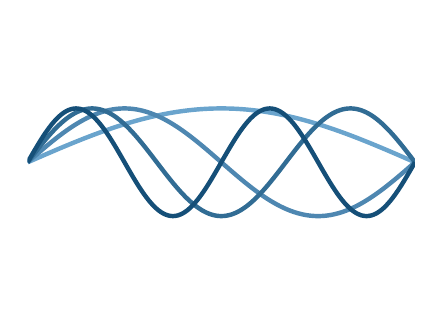
\begin{tikzpicture}
\begin{axis}[axis lines={none}, height={5cm}, width={6.5cm}, xmin={0}, xmax={1}, ymin={-2.5}, ymax={2.5}]
    \node at (0,-2.5) {};
    \node at (0,2.5) {};
    \node at (1,2.5) {};
    \node at (1,-2.5) {};
    \addplot[no markers, smooth, ultra thick, color={rgb,1:red,0.4157;green,0.6431;blue,0.8039}]
        coordinates {
            (0.0,0.0)
            (0.0125,0.03925981575906861)
            (0.025,0.07845909572784494)
            (0.0375,0.11753739745783764)
            (0.05,0.15643446504023087)
            (0.0625,0.19509032201612825)
            (0.075,0.2334453638559054)
            (0.0875,0.27144044986507426)
            (0.1,0.3090169943749474)
            (0.1125,0.34611705707749296)
            (0.125,0.3826834323650898)
            (0.1375,0.41865973753742813)
            (0.15,0.45399049973954675)
            (0.1625,0.4886212414969549)
            (0.175,0.5224985647159488)
            (0.1875,0.5555702330196022)
            (0.2,0.5877852522924731)
            (0.2125,0.619093949309834)
            (0.225,0.6494480483301837)
            (0.2375,0.6788007455329417)
            (0.25,0.7071067811865475)
            (0.2625,0.7343225094356856)
            (0.275,0.760405965600031)
            (0.2875,0.7853169308807448)
            (0.3,0.8090169943749475)
            (0.3125,0.8314696123025452)
            (0.325,0.8526401643540922)
            (0.3375,0.8724960070727971)
            (0.35,0.8910065241883678)
            (0.3625,0.9081431738250813)
            (0.375,0.9238795325112867)
            (0.3875,0.9381913359224842)
            (0.4,0.9510565162951535)
            (0.4125,0.9624552364536473)
            (0.425,0.9723699203976766)
            (0.4375,0.9807852804032304)
            (0.45,0.9876883405951378)
            (0.4625,0.9930684569549263)
            (0.475,0.996917333733128)
            (0.4875,0.9992290362407229)
            (0.5,1.0)
            (0.5125,0.9992290362407229)
            (0.525,0.996917333733128)
            (0.5375,0.9930684569549263)
            (0.55,0.9876883405951377)
            (0.5625,0.9807852804032304)
            (0.575,0.9723699203976767)
            (0.5875,0.9624552364536473)
            (0.6,0.9510565162951536)
            (0.6125,0.938191335922484)
            (0.625,0.9238795325112867)
            (0.6375,0.9081431738250815)
            (0.65,0.8910065241883679)
            (0.6625,0.8724960070727973)
            (0.675,0.8526401643540923)
            (0.6875,0.8314696123025453)
            (0.7,0.8090169943749475)
            (0.7125,0.7853169308807448)
            (0.725,0.7604059656000309)
            (0.7375,0.7343225094356854)
            (0.75,0.7071067811865476)
            (0.7625,0.678800745532942)
            (0.775,0.6494480483301838)
            (0.7875,0.6190939493098342)
            (0.8,0.5877852522924732)
            (0.8125,0.5555702330196022)
            (0.825,0.5224985647159489)
            (0.8375,0.48862124149695485)
            (0.85,0.45399049973954686)
            (0.8625,0.41865973753742797)
            (0.875,0.3826834323650899)
            (0.8875,0.3461170570774933)
            (0.9,0.3090169943749475)
            (0.9125,0.2714404498650746)
            (0.925,0.23344536385590553)
            (0.9375,0.1950903220161286)
            (0.95,0.15643446504023098)
            (0.9625,0.11753739745783755)
            (0.975,0.07845909572784507)
            (0.9875,0.039259815759068506)
            (1.0,1.2246467991473532e-16)
        }
        ;
    \addplot[no markers, smooth, ultra thick, color={rgb,1:red,0.3059;green,0.5294;blue,0.6941}]
        coordinates {
            (0.0,0.0)
            (0.0125,0.07845909572784494)
            (0.025,0.15643446504023087)
            (0.0375,0.2334453638559054)
            (0.05,0.3090169943749474)
            (0.0625,0.3826834323650898)
            (0.075,0.45399049973954675)
            (0.0875,0.5224985647159488)
            (0.1,0.5877852522924731)
            (0.1125,0.6494480483301837)
            (0.125,0.7071067811865475)
            (0.1375,0.760405965600031)
            (0.15,0.8090169943749475)
            (0.1625,0.8526401643540922)
            (0.175,0.8910065241883678)
            (0.1875,0.9238795325112867)
            (0.2,0.9510565162951535)
            (0.2125,0.9723699203976766)
            (0.225,0.9876883405951378)
            (0.2375,0.996917333733128)
            (0.25,1.0)
            (0.2625,0.996917333733128)
            (0.275,0.9876883405951377)
            (0.2875,0.9723699203976767)
            (0.3,0.9510565162951536)
            (0.3125,0.9238795325112867)
            (0.325,0.8910065241883679)
            (0.3375,0.8526401643540923)
            (0.35,0.8090169943749475)
            (0.3625,0.7604059656000309)
            (0.375,0.7071067811865476)
            (0.3875,0.6494480483301838)
            (0.4,0.5877852522924732)
            (0.4125,0.5224985647159489)
            (0.425,0.45399049973954686)
            (0.4375,0.3826834323650899)
            (0.45,0.3090169943749475)
            (0.4625,0.23344536385590553)
            (0.475,0.15643446504023098)
            (0.4875,0.07845909572784507)
            (0.5,1.2246467991473532e-16)
            (0.5125,-0.07845909572784437)
            (0.525,-0.15643446504023073)
            (0.5375,-0.23344536385590528)
            (0.55,-0.30901699437494773)
            (0.5625,-0.38268343236508967)
            (0.575,-0.45399049973954625)
            (0.5875,-0.5224985647159487)
            (0.6,-0.587785252292473)
            (0.6125,-0.6494480483301839)
            (0.625,-0.7071067811865475)
            (0.6375,-0.7604059656000306)
            (0.65,-0.8090169943749473)
            (0.6625,-0.8526401643540918)
            (0.675,-0.8910065241883678)
            (0.6875,-0.9238795325112865)
            (0.7,-0.9510565162951535)
            (0.7125,-0.9723699203976767)
            (0.725,-0.9876883405951377)
            (0.7375,-0.996917333733128)
            (0.75,-1.0)
            (0.7625,-0.9969173337331281)
            (0.775,-0.9876883405951378)
            (0.7875,-0.9723699203976768)
            (0.8,-0.9510565162951536)
            (0.8125,-0.9238795325112866)
            (0.825,-0.891006524188368)
            (0.8375,-0.8526401643540921)
            (0.85,-0.8090169943749476)
            (0.8625,-0.7604059656000308)
            (0.875,-0.7071067811865477)
            (0.8875,-0.6494480483301841)
            (0.9,-0.5877852522924734)
            (0.9125,-0.5224985647159495)
            (0.925,-0.45399049973954697)
            (0.9375,-0.3826834323650904)
            (0.95,-0.3090169943749476)
            (0.9625,-0.2334453638559052)
            (0.975,-0.15643446504023112)
            (0.9875,-0.07845909572784475)
            (1.0,-2.4492935982947064e-16)
        }
        ;
    \addplot[no markers, smooth, ultra thick, color={rgb,1:red,0.1922;green,0.4235;blue,0.5804}]
        coordinates {
            (0.0,0.0)
            (0.0125,0.11753739745783764)
            (0.025,0.2334453638559054)
            (0.0375,0.34611705707749296)
            (0.05,0.45399049973954675)
            (0.0625,0.5555702330196022)
            (0.075,0.6494480483301837)
            (0.0875,0.7343225094356856)
            (0.1,0.8090169943749475)
            (0.1125,0.8724960070727971)
            (0.125,0.9238795325112867)
            (0.1375,0.9624552364536473)
            (0.15,0.9876883405951378)
            (0.1625,0.9992290362407229)
            (0.175,0.996917333733128)
            (0.1875,0.9807852804032304)
            (0.2,0.9510565162951536)
            (0.2125,0.9081431738250815)
            (0.225,0.8526401643540923)
            (0.2375,0.7853169308807452)
            (0.25,0.7071067811865476)
            (0.2625,0.6190939493098339)
            (0.275,0.5224985647159489)
            (0.2875,0.4186597375374284)
            (0.3,0.3090169943749475)
            (0.3125,0.1950903220161286)
            (0.325,0.07845909572784507)
            (0.3375,-0.03925981575906871)
            (0.35,-0.15643446504023073)
            (0.3625,-0.27144044986507393)
            (0.375,-0.38268343236508967)
            (0.3875,-0.488621241496955)
            (0.4,-0.587785252292473)
            (0.4125,-0.6788007455329415)
            (0.425,-0.7604059656000306)
            (0.4375,-0.8314696123025452)
            (0.45,-0.8910065241883678)
            (0.4625,-0.938191335922484)
            (0.475,-0.9723699203976764)
            (0.4875,-0.9930684569549263)
            (0.5,-1.0)
            (0.5125,-0.9930684569549263)
            (0.525,-0.9723699203976766)
            (0.5375,-0.9381913359224842)
            (0.55,-0.891006524188368)
            (0.5625,-0.8314696123025455)
            (0.575,-0.7604059656000314)
            (0.5875,-0.6788007455329417)
            (0.6,-0.5877852522924734)
            (0.6125,-0.4886212414969546)
            (0.625,-0.3826834323650904)
            (0.6375,-0.2714404498650751)
            (0.65,-0.15643446504023112)
            (0.6625,-0.039259815759069075)
            (0.675,0.07845909572784514)
            (0.6875,0.19509032201612825)
            (0.7,0.3090169943749472)
            (0.7125,0.41865973753742763)
            (0.725,0.5224985647159482)
            (0.7375,0.619093949309834)
            (0.75,0.7071067811865474)
            (0.7625,0.7853169308807446)
            (0.775,0.8526401643540923)
            (0.7875,0.9081431738250813)
            (0.8,0.9510565162951535)
            (0.8125,0.9807852804032303)
            (0.825,0.996917333733128)
            (0.8375,0.9992290362407229)
            (0.85,0.9876883405951379)
            (0.8625,0.9624552364536474)
            (0.875,0.9238795325112867)
            (0.8875,0.8724960070727976)
            (0.9,0.8090169943749476)
            (0.9125,0.7343225094356853)
            (0.925,0.6494480483301842)
            (0.9375,0.5555702330196023)
            (0.95,0.4539904997395479)
            (0.9625,0.3461170570774935)
            (0.975,0.23344536385590534)
            (0.9875,0.11753739745783691)
            (1.0,3.6739403974420594e-16)
        }
        ;
    \addplot[no markers, smooth, ultra thick, color={rgb,1:red,0.0824;green,0.3098;blue,0.4706}]
        coordinates {
            (0.0,0.0)
            (0.0125,0.15643446504023087)
            (0.025,0.3090169943749474)
            (0.0375,0.45399049973954675)
            (0.05,0.5877852522924731)
            (0.0625,0.7071067811865475)
            (0.075,0.8090169943749475)
            (0.0875,0.8910065241883678)
            (0.1,0.9510565162951535)
            (0.1125,0.9876883405951378)
            (0.125,1.0)
            (0.1375,0.9876883405951377)
            (0.15,0.9510565162951536)
            (0.1625,0.8910065241883679)
            (0.175,0.8090169943749475)
            (0.1875,0.7071067811865476)
            (0.2,0.5877852522924732)
            (0.2125,0.45399049973954686)
            (0.225,0.3090169943749475)
            (0.2375,0.15643446504023098)
            (0.25,1.2246467991473532e-16)
            (0.2625,-0.15643446504023073)
            (0.275,-0.30901699437494773)
            (0.2875,-0.45399049973954625)
            (0.3,-0.587785252292473)
            (0.3125,-0.7071067811865475)
            (0.325,-0.8090169943749473)
            (0.3375,-0.8910065241883678)
            (0.35,-0.9510565162951535)
            (0.3625,-0.9876883405951377)
            (0.375,-1.0)
            (0.3875,-0.9876883405951378)
            (0.4,-0.9510565162951536)
            (0.4125,-0.891006524188368)
            (0.425,-0.8090169943749476)
            (0.4375,-0.7071067811865477)
            (0.45,-0.5877852522924734)
            (0.4625,-0.45399049973954697)
            (0.475,-0.3090169943749476)
            (0.4875,-0.15643446504023112)
            (0.5,-2.4492935982947064e-16)
            (0.5125,0.15643446504022973)
            (0.525,0.3090169943749472)
            (0.5375,0.4539904997395466)
            (0.55,0.5877852522924736)
            (0.5625,0.7071067811865474)
            (0.575,0.8090169943749468)
            (0.5875,0.8910065241883678)
            (0.6,0.9510565162951535)
            (0.6125,0.9876883405951378)
            (0.625,1.0)
            (0.6375,0.9876883405951379)
            (0.65,0.9510565162951536)
            (0.6625,0.8910065241883685)
            (0.675,0.8090169943749476)
            (0.6875,0.7071067811865483)
            (0.7,0.5877852522924734)
            (0.7125,0.4539904997395463)
            (0.725,0.3090169943749478)
            (0.7375,0.15643446504023034)
            (0.75,3.6739403974420594e-16)
            (0.7625,-0.15643446504022962)
            (0.775,-0.30901699437494706)
            (0.7875,-0.45399049973954564)
            (0.8,-0.5877852522924728)
            (0.8125,-0.7071067811865479)
            (0.825,-0.8090169943749472)
            (0.8375,-0.8910065241883681)
            (0.85,-0.9510565162951534)
            (0.8625,-0.9876883405951378)
            (0.875,-1.0)
            (0.8875,-0.9876883405951379)
            (0.9,-0.9510565162951538)
            (0.9125,-0.8910065241883685)
            (0.925,-0.8090169943749477)
            (0.9375,-0.7071067811865485)
            (0.95,-0.5877852522924735)
            (0.9625,-0.4539904997395464)
            (0.975,-0.3090169943749479)
            (0.9875,-0.15643446504023048)
            (1.0,-4.898587196589413e-16)
        }
        ;
\end{axis}
\end{tikzpicture}
\end{document}

\caption{Karhunen--Loève basis}
\end{subfigure}
\begin{subfigure}{0.49\textwidth}
\documentclass[tikz]{standalone}
\usepackage{pgfplots}
\pgfplotsset{compat=1.17}
\usepgfplotslibrary{external}
\usepgfplotslibrary{groupplots}
\usepgfplotslibrary{fillbetween}
\usetikzlibrary{fadings}
\begin{document}
\tikzsetnextfilename{figures/tex/gp-kl-samples.pdf}
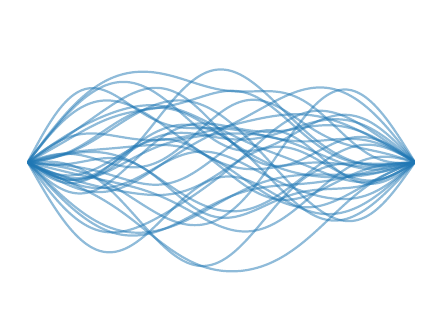
\begin{tikzpicture}
\begin{axis}[axis lines={none}, height={5cm}, width={6.5cm}, xmin={0}, xmax={1}, ymin={-1}, ymax={1}]
    \node at (0,-1) {};
    \node at (0,1) {};
    \node at (1,1) {};
    \node at (1,-1) {};
    \addplot[no markers, smooth, thick, color={rgb,1:red,0.1216;green,0.4667;blue,0.7059}, opacity={0.5}]
        coordinates {
            (0.0,0.0)
            (0.0125,-0.03380796886587739)
            (0.025,-0.06689109114398441)
            (0.0375,-0.0985406134994172)
            (0.05,-0.12807962531475114)
            (0.0625,-0.1548781200822741)
            (0.075,-0.17836702486582137)
            (0.0875,-0.1980508579253363)
            (0.1,-0.2135186854285231)
            (0.1125,-0.2244530694185271)
            (0.125,-0.2306367339414423)
            (0.1375,-0.23195672647803675)
            (0.15,-0.22840591803542099)
            (0.1625,-0.22008176605229338)
            (0.175,-0.20718235636311816)
            (0.1875,-0.18999983884928928)
            (0.2,-0.1689114698065583)
            (0.2125,-0.14436856556952093)
            (0.225,-0.11688374976284194)
            (0.2375,-0.087016934792284)
            (0.25,-0.055360512532549436)
            (0.2625,-0.022524237419102436)
            (0.275,0.01087973247724004)
            (0.2875,0.04425121169001926)
            (0.3,0.07701541556911445)
            (0.3125,0.10863514661963472)
            (0.325,0.1386215215587423)
            (0.3375,0.16654309585888524)
            (0.35,0.19203330810671385)
            (0.3625,0.2147962186698847)
            (0.375,0.23461055325937655)
            (0.3875,0.2513320817109335)
            (0.4,0.26489436773527136)
            (0.4125,0.27530792055995457)
            (0.425,0.2826577697832553)
            (0.4375,0.2870994765112226)
            (0.45,0.288853592886409)
            (0.4625,0.2881985933522728)
            (0.475,0.2854623276256525)
            (0.4875,0.28101208836301994)
            (0.5,0.27524344447926746)
            (0.5125,0.26856806024588187)
            (0.525,0.2614007949125371)
            (0.5375,0.25414645052797596)
            (0.55,0.24718659911557475)
            (0.5625,0.2408669668172594)
            (0.575,0.235485875498095)
            (0.5875,0.2312842367622543)
            (0.6,0.22843755677705574)
            (0.6125,0.22705034269750282)
            (0.625,0.22715320540432296)
            (0.6375,0.2287028337177011)
            (0.65,0.23158487926063492)
            (0.6625,0.23561964721737222)
            (0.675,0.24057034564845872)
            (0.6875,0.2461535141349319)
            (0.7,0.2520511400404243)
            (0.7125,0.25792388503671243)
            (0.725,0.26342479137606206)
            (0.7375,0.26821282018462805)
            (0.75,0.2719655938892701)
            (0.7625,0.27439077045123555)
            (0.775,0.27523556474411165)
            (0.7875,0.2742940465339176)
            (0.8,0.2714119778171983)
            (0.8125,0.2664890963257442)
            (0.825,0.25947889779956673)
            (0.8375,0.2503861081366174)
            (0.85,0.23926215928363806)
            (0.8625,0.22619908236597727)
            (0.875,0.2113223022461646)
            (0.8875,0.19478285554299768)
            (0.9,0.17674955737285497)
            (0.9125,0.1574016111757067)
            (0.925,0.13692209364274754)
            (0.9375,0.11549265766770953)
            (0.95,0.09328968679585374)
            (0.9625,0.07048201251466955)
            (0.975,0.04723017935880627)
            (0.9875,0.0236871208437627)
            (1.0,7.394304450038177e-17)
        }
        ;
    \addplot[no markers, smooth, thick, color={rgb,1:red,0.1216;green,0.4667;blue,0.7059}, opacity={0.5}]
        coordinates {
            (0.0,0.0)
            (0.0125,0.06785330730815943)
            (0.025,0.13456901745868752)
            (0.0375,0.19904062592559085)
            (0.05,0.26022277515432146)
            (0.0625,0.3171592726592928)
            (0.075,0.36900815365141243)
            (0.0875,0.4150629822862373)
            (0.1,0.4547697281809916)
            (0.1125,0.48773872007173)
            (0.125,0.5137513589963154)
            (0.1375,0.5327614614649654)
            (0.15,0.5448912910666092)
            (0.1625,0.5504225176716622)
            (0.175,0.549782510427865)
            (0.1875,0.543526518710527)
            (0.2,0.5323164198212579)
            (0.2125,0.5168968104381318)
            (0.225,0.4980692886366152)
            (0.2375,0.476665813775714)
            (0.25,0.4535220426121008)
            (0.2625,0.4294515223391081)
            (0.275,0.4052215761285779)
            (0.2875,0.38153164597202344)
            (0.3,0.3589947634145172)
            (0.3125,0.3381227038239005)
            (0.325,0.31931524726071925)
            (0.3375,0.30285382241368275)
            (0.35,0.28889965355993036)
            (0.3625,0.27749636874652406)
            (0.375,0.26857686552007093)
            (0.3875,0.26197407412800866)
            (0.4,0.2574351130275457)
            (0.4125,0.2546382036821736)
            (0.425,0.2532116067121028)
            (0.4375,0.2527537646854352)
            (0.45,0.2528537925248206)
            (0.4625,0.2531114478001015)
            (0.475,0.2531557417261489)
            (0.4875,0.25266141739715337)
            (0.5,0.2513626226905431)
            (0.5125,0.249063237471287)
            (0.525,0.2456434724964136)
            (0.5375,0.2410625334294859)
            (0.55,0.23535732903960913)
            (0.5625,0.22863738860069832)
            (0.575,0.22107633009940963)
            (0.5875,0.21290037882779936)
            (0.6,0.20437456694946107)
            (0.6125,0.19578734185842253)
            (0.625,0.18743436974093447)
            (0.6375,0.17960233815042773)
            (0.65,0.1725535375452878)
            (0.6625,0.16651193902158096)
            (0.675,0.16165138858455658)
            (0.6875,0.15808641384925862)
            (0.7,0.15586599506260085)
            (0.7125,0.1549704976310822)
            (0.725,0.15531180692151214)
            (0.7375,0.15673655651310978)
            (0.75,0.1590322058257529)
            (0.7625,0.16193560816347388)
            (0.775,0.16514361995699894)
            (0.7875,0.16832523873165559)
            (0.8,0.171134721583546)
            (0.8125,0.17322512657706646)
            (0.825,0.17426173399513203)
            (0.8375,0.17393483933440881)
            (0.85,0.17197146134634)
            (0.8625,0.16814557212516693)
            (0.875,0.16228652824932527)
            (0.8875,0.1542854587156164)
            (0.9,0.14409944384170914)
            (0.9125,0.1317533970235096)
            (0.925,0.11733963634934805)
            (0.9375,0.10101520418361094)
            (0.95,0.08299705886447167)
            (0.9625,0.06355532274882277)
            (0.975,0.04300482422341537)
            (0.9875,0.02169521726718387)
            (1.0,6.786424492935426e-17)
        }
        ;
    \addplot[no markers, smooth, thick, color={rgb,1:red,0.1216;green,0.4667;blue,0.7059}, opacity={0.5}]
        coordinates {
            (0.0,0.0)
            (0.0125,0.004729293066739817)
            (0.025,0.009868162784691069)
            (0.0375,0.015809016811798693)
            (0.05,0.022910670482301183)
            (0.0625,0.031483377848113205)
            (0.075,0.04177595375808649)
            (0.0875,0.05396552017765549)
            (0.1,0.06815028041154039)
            (0.1125,0.08434557609117636)
            (0.125,0.10248332171993911)
            (0.1375,0.12241474901978007)
            (0.15,0.1439162373977267)
            (0.1625,0.16669786642551845)
            (0.175,0.19041420935624453)
            (0.1875,0.21467680003533607)
            (0.2,0.23906765380475758)
            (0.2125,0.263153208491733)
            (0.225,0.28649807404495065)
            (0.2375,0.3086780359019312)
            (0.25,0.32929184234271464)
            (0.2625,0.3479714124617959)
            (0.275,0.3643902201051515)
            (0.2875,0.3782697306590798)
            (0.3,0.38938388263528956)
            (0.3125,0.3975617063123235)
            (0.325,0.4026882507951916)
            (0.3375,0.4047040446180551)
            (0.35,0.4036033419751031)
            (0.3625,0.3994314080532064)
            (0.375,0.39228107643132476)
            (0.3875,0.38228877471903133)
            (0.4,0.3696301683792053)
            (0.4125,0.3545155242875158)
            (0.425,0.3371848518780317)
            (0.4375,0.3179028463897962)
            (0.45,0.29695363967143423)
            (0.4625,0.27463536098509234)
            (0.475,0.25125452279244)
            (0.4875,0.2271202720285912)
            (0.5,0.20253858160789515)
            (0.5125,0.17780649448397012)
            (0.525,0.15320656771495922)
            (0.5375,0.12900169117307037)
            (0.55,0.10543047024646188)
            (0.5625,0.08270336104071198)
            (0.575,0.060999728917373056)
            (0.5875,0.04046596732380573)
            (0.6,0.02121476616115165)
            (0.6125,0.003325561252460941)
            (0.625,-0.013153866352920991)
            (0.6375,-0.02820473519637684)
            (0.65,-0.041833703727184035)
            (0.6625,-0.05406860515712052)
            (0.675,-0.06495371035638123)
            (0.6875,-0.07454477146167743)
            (0.7,-0.08290410204423662)
            (0.7125,-0.09009593753100163)
            (0.725,-0.09618229388945665)
            (0.7375,-0.10121950601780601)
            (0.75,-0.1052555829570209)
            (0.7625,-0.10832846822390238)
            (0.775,-0.11046524334923992)
            (0.7875,-0.11168226379212365)
            (0.8,-0.11198617096851747)
            (0.8125,-0.11137568380679692)
            (0.825,-0.10984403915600087)
            (0.8375,-0.10738192326743647)
            (0.85,-0.10398071693286683)
            (0.8625,-0.0996358650374944)
            (0.875,-0.09435017755140014)
            (0.8875,-0.08813687356561692)
            (0.9,-0.08102219300645513)
            (0.9125,-0.07304742206410962)
            (0.925,-0.06427020775387733)
            (0.9375,-0.05476507354524854)
            (0.95,-0.044623090260477685)
            (0.9625,-0.033950702508357404)
            (0.975,-0.022867758318091166)
            (0.9875,-0.011504835540070325)
            (1.0,-3.595223553930849e-17)
        }
        ;
    \addplot[no markers, smooth, thick, color={rgb,1:red,0.1216;green,0.4667;blue,0.7059}, opacity={0.5}]
        coordinates {
            (0.0,0.0)
            (0.0125,0.0021603792148044065)
            (0.025,0.003954099851348791)
            (0.0375,0.005019695430728969)
            (0.05,0.005006097644200619)
            (0.0625,0.00357786274522242)
            (0.075,0.0004204100455670017)
            (0.0875,-0.004754755902868786)
            (0.1,-0.01220489183223891)
            (0.1125,-0.02215100883857919)
            (0.125,-0.03477311426263724)
            (0.1375,-0.050205825344226795)
            (0.15,-0.06853449224039124)
            (0.1625,-0.08979197446272032)
            (0.175,-0.11395621167529334)
            (0.1875,-0.14094871647487198)
            (0.2,-0.17063409354138312)
            (0.2125,-0.20282065764801743)
            (0.225,-0.2372621846005251)
            (0.2375,-0.2736607871116677)
            (0.25,-0.31167086526285287)
            (0.2625,-0.3509040420610458)
            (0.275,-0.39093496194117616)
            (0.2875,-0.43130780657244)
            (0.3,-0.4715433697565609)
            (0.3125,-0.5111465321453134)
            (0.325,-0.5496139862528726)
            (0.3375,-0.5864420808295816)
            (0.35,-0.6211346780408358)
            (0.3625,-0.6532109432270534)
            (0.375,-0.6822130111324831)
            (0.3875,-0.7077134903599266)
            (0.4,-0.7293227760792362)
            (0.4125,-0.746696137465278)
            (0.425,-0.7595405302335049)
            (0.4375,-0.7676210569430142)
            (0.45,-0.770766961125025)
            (0.4625,-0.7688769999701687)
            (0.475,-0.7619239996139698)
            (0.4875,-0.7499583629388045)
            (0.5,-0.7331102781566345)
            (0.5125,-0.7115903724130715)
            (0.525,-0.6856885720530185)
            (0.5375,-0.6557709719164343)
            (0.55,-0.6222745797750732)
            (0.5625,-0.5856998861441842)
            (0.575,-0.5466013094077194)
            (0.5875,-0.5055756749099265)
            (0.6,-0.4632489966400444)
            (0.6125,-0.4202619331702624)
            (0.625,-0.3772543777307553)
            (0.6375,-0.334849708922753)
            (0.65,-0.293639268476805)
            (0.6625,-0.2541676426740918)
            (0.675,-0.2169193038925234)
            (0.6875,-0.18230711980388037)
            (0.7,-0.15066316359685974)
            (0.7125,-0.12223216431034944)
            (0.725,-0.09716782794656055)
            (0.7375,-0.07553214384174622)
            (0.75,-0.05729767292153587)
            (0.7625,-0.042352700400727375)
            (0.775,-0.030509029679595796)
            (0.7875,-0.021512100034409048)
            (0.8,-0.015053030560163525)
            (0.8125,-0.01078212820503265)
            (0.825,-0.008323349543455188)
            (0.8375,-0.007289174737916278)
            (0.85,-0.00729533839315168)
            (0.8625,-0.007974866177469923)
            (0.875,-0.008990888658702468)
            (0.8875,-0.010047745161738791)
            (0.9,-0.010899950666017743)
            (0.9125,-0.011358677291345962)
            (0.925,-0.011295497353713928)
            (0.9375,-0.010643244785022323)
            (0.95,-0.009393972151362081)
            (0.9625,-0.007594106629393673)
            (0.975,-0.005337034169798204)
            (0.9875,-0.002753460113579151)
            (1.0,-8.680790104241566e-18)
        }
        ;
    \addplot[no markers, smooth, thick, color={rgb,1:red,0.1216;green,0.4667;blue,0.7059}, opacity={0.5}]
        coordinates {
            (0.0,0.0)
            (0.0125,-0.04000693946930761)
            (0.025,-0.07979988014298942)
            (0.0375,-0.11916532602181676)
            (0.05,-0.15789087195737816)
            (0.0625,-0.1957659531426628)
            (0.075,-0.23258281507577974)
            (0.0875,-0.2681377397407713)
            (0.1,-0.3022325368668665)
            (0.1125,-0.33467628155432955)
            (0.125,-0.3652872541756456)
            (0.1375,-0.3938950178043847)
            (0.15,-0.4203425543795287)
            (0.1625,-0.44448837443353567)
            (0.175,-0.4662085166325985)
            (0.1875,-0.48539836184843055)
            (0.2,-0.5019742005124775)
            (0.2125,-0.5158745095907166)
            (0.225,-0.5270609144153934)
            (0.2375,-0.5355188286201804)
            (0.25,-0.541257780652636)
            (0.2625,-0.5443114463921793)
            (0.275,-0.5447374135178791)
            (0.2875,-0.5426167043415593)
            (0.3,-0.5380530803499599)
            (0.3125,-0.5311721446779027)
            (0.325,-0.5221202494843098)
            (0.3375,-0.5110632051947669)
            (0.35,-0.4981847792547364)
            (0.3625,-0.4836849646864277)
            (0.375,-0.46777799437266837)
            (0.3875,-0.4506900762965464)
            (0.4,-0.43265682831191626)
            (0.4125,-0.41392039847063555)
            (0.425,-0.39472626829290497)
            (0.4375,-0.37531975123256034)
            (0.45,-0.3559422163834068)
            (0.4625,-0.33682708746971485)
            (0.475,-0.3181956884912716)
            (0.4875,-0.30025302902173145)
            (0.5,-0.28318364289042164)
            (0.5125,-0.2671476124444289)
            (0.525,-0.2522769252769355)
            (0.5375,-0.23867231962258942)
            (0.55,-0.22640077698283068)
            (0.5625,-0.2154938145345088)
            (0.575,-0.2059467144024804)
            (0.5875,-0.19771880135486686)
            (0.6,-0.19073484498958737)
            (0.6125,-0.1848876178941129)
            (0.625,-0.18004158929738173)
            (0.6375,-0.1760376769399956)
            (0.65,-0.17269892152614102)
            (0.6625,-0.16983689196074458)
            (0.675,-0.167258579628098)
            (0.6875,-0.16477350015502606)
            (0.7,-0.16220069491052522)
            (0.7125,-0.15937531465068833)
            (0.725,-0.1561544759097345)
            (0.7375,-0.15242210741851442)
            (0.75,-0.14809254812984457)
            (0.7625,-0.14311271817405058)
            (0.775,-0.13746275592440568)
            (0.7875,-0.1311550940629467)
            (0.8,-0.12423203023620429)
            (0.8125,-0.11676192846536826)
            (0.825,-0.10883426094312935)
            (0.8375,-0.10055376171075385)
            (0.85,-0.09203401025369959)
            (0.8625,-0.0833907915937364)
            (0.875,-0.07473558846920032)
            (0.8875,-0.06616955038410638)
            (0.9,-0.05777825456206666)
            (0.9125,-0.04962752713234558)
            (0.925,-0.04176053208164858)
            (0.9375,-0.03419626420101263)
            (0.95,-0.02692950447739989)
            (0.9625,-0.019932216379014094)
            (0.975,-0.013156283505691506)
            (0.9875,-0.006537417143851321)
            (1.0,-2.0339734980947138e-17)
        }
        ;
    \addplot[no markers, smooth, thick, color={rgb,1:red,0.1216;green,0.4667;blue,0.7059}, opacity={0.5}]
        coordinates {
            (0.0,0.0)
            (0.0125,0.027525341130523868)
            (0.025,0.05453030648313176)
            (0.0375,0.08051228445297177)
            (0.05,0.105003448898551)
            (0.0625,0.12758633136948838)
            (0.075,0.14790730927769416)
            (0.0875,0.16568747642612597)
            (0.1,0.18073048797986407)
            (0.1125,0.19292711470048116)
            (0.125,0.20225639316916844)
            (0.1375,0.20878341175286608)
            (0.15,0.21265391854889906)
            (0.1625,0.21408607061606544)
            (0.175,0.21335975773993268)
            (0.1875,0.21080402440185778)
            (0.2,0.2067831775553806)
            (0.2125,0.2016822036777803)
            (0.225,0.19589212605699893)
            (0.2375,0.1897959132222567)
            (0.25,0.18375550362308807)
            (0.2625,0.1781004427131582)
            (0.275,0.1731185398017493)
            (0.2875,0.16904884730035172)
            (0.3,0.16607714875599752)
            (0.3125,0.16433401924830637)
            (0.325,0.1638953976598923)
            (0.3375,0.16478549062565054)
            (0.35,0.16698171835799888)
            (0.3625,0.1704213186414077)
            (0.375,0.17500915227259595)
            (0.3875,0.18062620549763275)
            (0.4,0.18713826582424672)
            (0.4125,0.1944042587361976)
            (0.425,0.20228377430218508)
            (0.4375,0.2106433825002289)
            (0.45,0.21936143033090313)
            (0.4625,0.22833112667629213)
            (0.475,0.2374618450318354)
            (0.4875,0.24667870126443942)
            (0.5,0.2559205845116145)
            (0.5125,0.26513692550573853)
            (0.525,0.27428357016231336)
            (0.5375,0.2833181809668607)
            (0.55,0.29219561043515785)
            (0.5625,0.30086367816252835)
            (0.575,0.3092597369257598)
            (0.5875,0.3173083378683127)
            (0.6,0.32492020631842106)
            (0.6125,0.3319926265017524)
            (0.625,0.3384112147701119)
            (0.6375,0.34405294682564824)
            (0.65,0.3487902041574878)
            (0.6625,0.35249552660721317)
            (0.675,0.35504670770989494)
            (0.6875,0.35633185074431334)
            (0.7,0.3562540169607616)
            (0.7125,0.35473514106994214)
            (0.725,0.35171895799124236)
            (0.7375,0.34717277217000203)
            (0.75,0.34108799814220114)
            (0.7625,0.33347949948942296)
            (0.775,0.32438384416050875)
            (0.7875,0.31385666966551384)
            (0.8,0.30196940594857163)
            (0.8125,0.2888056331527757)
            (0.825,0.2744573548657762)
            (0.8375,0.2590214461863962)
            (0.85,0.24259649378973913)
            (0.8625,0.22528018763764243)
            (0.875,0.20716735782924203)
            (0.8875,0.18834868251839038)
            (0.9,0.16891003074124478)
            (0.9125,0.14893235328534138)
            (0.925,0.1284919996847563)
            (0.9375,0.10766132235323476)
            (0.95,0.0865094299253816)
            (0.9625,0.06510296914289725)
            (0.975,0.043506844396363854)
            (0.9875,0.021784821321901723)
            (1.0,6.797199443184857e-17)
        }
        ;
    \addplot[no markers, smooth, thick, color={rgb,1:red,0.1216;green,0.4667;blue,0.7059}, opacity={0.5}]
        coordinates {
            (0.0,0.0)
            (0.0125,0.004984029265112188)
            (0.025,0.010277892850899075)
            (0.0375,0.016180282529331836)
            (0.05,0.022968100313175234)
            (0.0625,0.030886771902252263)
            (0.075,0.04014192828184587)
            (0.0875,0.05089278158921561)
            (0.1,0.06324742235449768)
            (0.1125,0.07726015569775747)
            (0.125,0.0929308817490024)
            (0.1375,0.1102064181649371)
            (0.15,0.12898356724000745)
            (0.1625,0.1491136526894402)
            (0.175,0.17040819607839644)
            (0.1875,0.19264537258655015)
            (0.2,0.21557688086458424)
            (0.2125,0.2389348807785656)
            (0.225,0.26243869276829124)
            (0.2375,0.2858010089215625)
            (0.25,0.3087334333077617)
            (0.2625,0.3309512417800713)
            (0.275,0.35217732352045433)
            (0.2875,0.3721453326927286)
            (0.3,0.3906021341350594)
            (0.3125,0.407309668608471)
            (0.325,0.42204638853597926)
            (0.3375,0.43460842357080287)
            (0.35,0.4448106271919282)
            (0.3625,0.45248763252602503)
            (0.375,0.4574950104713032)
            (0.3875,0.45971057952344274)
            (0.4,0.45903586863819934)
            (0.4125,0.45539768648862367)
            (0.425,0.4487497070916789)
            (0.4375,0.43907394721622417)
            (0.45,0.42638198888299766)
            (0.4625,0.4107157933829222)
            (0.475,0.3921479631686986)
            (0.4875,0.37078133492824483)
            (0.5,0.34674782980924573)
            (0.5125,0.32020654224582873)
            (0.525,0.2913411127820146)
            (0.5375,0.2603564971050364)
            (0.55,0.22747530677701946)
            (0.5625,0.19293395017043755)
            (0.575,0.1569788384904414)
            (0.5875,0.11986293613609793)
            (0.6,0.08184292330491996)
            (0.6125,0.04317720018234411)
            (0.625,0.004124897360688912)
            (0.6375,-0.03505402990969383)
            (0.65,-0.0740976490716184)
            (0.6625,-0.11273997521191209)
            (0.675,-0.15070821780915775)
            (0.6875,-0.1877196889134073)
            (0.7,-0.22347878518121272)
            (0.7125,-0.2576744979820311)
            (0.725,-0.28997891070503024)
            (0.7375,-0.3200471077068081)
            (0.75,-0.34751884588522264)
            (0.7625,-0.3720222320649543)
            (0.775,-0.39317951490361824)
            (0.7875,-0.4106149490975208)
            (0.8,-0.423964534107261)
            (0.8125,-0.43288728173635915)
            (0.825,-0.43707753829881074)
            (0.8375,-0.43627778767011566)
            (0.85,-0.4302912984868066)
            (0.8625,-0.4189939562280693)
            (0.875,-0.4023446395883261)
            (0.8875,-0.3803935579115168)
            (0.9,-0.3532880572256805)
            (0.9125,-0.32127551926023623)
            (0.925,-0.2847031122195257)
            (0.9375,-0.24401429517403928)
            (0.95,-0.19974212133436764)
            (0.9625,-0.1524995218989745)
            (0.975,-0.1029668757948501)
            (0.9875,-0.05187727724575809)
            (1.0,-1.6218446391432418e-16)
        }
        ;
    \addplot[no markers, smooth, thick, color={rgb,1:red,0.1216;green,0.4667;blue,0.7059}, opacity={0.5}]
        coordinates {
            (0.0,0.0)
            (0.0125,0.02345102962927287)
            (0.025,0.04694186393472496)
            (0.0375,0.0705120676932677)
            (0.05,0.09420049210965825)
            (0.0625,0.11804435654002672)
            (0.075,0.14207771885950082)
            (0.0875,0.16632922945827106)
            (0.1,0.19081913838189712)
            (0.1125,0.21555560658866765)
            (0.125,0.24053045426454644)
            (0.1375,0.2657145551503109)
            (0.15,0.29105314987367203)
            (0.1625,0.3164613982090061)
            (0.175,0.34182051613482717)
            (0.1875,0.3669748461713948)
            (0.2,0.39173018806491167)
            (0.2125,0.41585367241645893)
            (0.225,0.4390753948606307)
            (0.2375,0.46109194673217807)
            (0.25,0.4815718846791475)
            (0.2625,0.5001630818850028)
            (0.275,0.516501803188175)
            (0.2875,0.5302232510295157)
            (0.3,0.5409732439229775)
            (0.3125,0.5484206183750368)
            (0.325,0.5522698922597167)
            (0.3375,0.5522736949147552)
            (0.35,0.5482444579122276)
            (0.3625,0.5400648708095066)
            (0.375,0.5276966375357046)
            (0.3875,0.5111871199837233)
            (0.4,0.4906735238091622)
            (0.4125,0.4663843648434902)
            (0.425,0.4386380499720645)
            (0.4375,0.4078385105322803)
            (0.45,0.3744679356696767)
            (0.4625,0.3390767637743165)
            (0.475,0.30227119796306906)
            (0.4875,0.2646986122234879)
            (0.5,0.22703130384425302)
            (0.5125,0.1899491207637811)
            (0.525,0.15412154544576795)
            (0.5375,0.12018984644910166)
            (0.55,0.08874991257574207)
            (0.5625,0.06033636120565236)
            (0.575,0.035408462538218784)
            (0.5875,0.014338346993715103)
            (0.6,-0.002598132316829333)
            (0.6125,-0.015227621184792895)
            (0.625,-0.02348242948837379)
            (0.6375,-0.027400622235343)
            (0.65,-0.027123136691211917)
            (0.6625,-0.022888132379530142)
            (0.675,-0.015022870348435753)
            (0.6875,-0.003933486736674532)
            (0.7,0.0099069288315745)
            (0.7125,0.02597151736634292)
            (0.725,0.04369366410947053)
            (0.7375,0.06248142676927734)
            (0.75,0.08173199604800244)
            (0.7625,0.1008458480795314)
            (0.775,0.11924029498813668)
            (0.7875,0.13636218668554576)
            (0.8,0.15169956084565223)
            (0.8125,0.16479207650749228)
            (0.825,0.17524009898356865)
            (0.8375,0.18271232988382077)
            (0.85,0.18695189723857109)
            (0.8625,0.18778083867266357)
            (0.875,0.1851029273676112)
            (0.8875,0.17890480808570233)
            (0.9,0.1692554303839861)
            (0.9125,0.15630378930828986)
            (0.925,0.14027501064923892)
            (0.9375,0.12146484791870743)
            (0.95,0.10023269064292187)
            (0.9625,0.07699321701217951)
            (0.975,0.05220685676454857)
            (0.9875,0.026369260719358155)
            (1.0,8.249838096910789e-17)
        }
        ;
    \addplot[no markers, smooth, thick, color={rgb,1:red,0.1216;green,0.4667;blue,0.7059}, opacity={0.5}]
        coordinates {
            (0.0,0.0)
            (0.0125,0.026420628923923568)
            (0.025,0.05268038290025467)
            (0.0375,0.07862450468857785)
            (0.05,0.10410998623801873)
            (0.0625,0.12901026681566127)
            (0.075,0.15321862575809786)
            (0.0875,0.176650003003636)
            (0.1,0.1992411074826909)
            (0.1125,0.2209488120123053)
            (0.125,0.24174697249686464)
            (0.1375,0.2616219378267647)
            (0.15,0.28056712454155724)
            (0.1625,0.2985771083917927)
            (0.175,0.3156417270883677)
            (0.1875,0.3317406913922191)
            (0.2,0.3468391651223865)
            (0.2125,0.36088470175171816)
            (0.225,0.37380582211069224)
            (0.2375,0.3855123928790113)
            (0.25,0.3958978292524743)
            (0.2625,0.40484300844481524)
            (0.275,0.4122216543259853)
            (0.2875,0.41790684715010284)
            (0.3,0.42177823363710987)
            (0.3125,0.42372946668595185)
            (0.325,0.4236753928125597)
            (0.3375,0.42155852814009914)
            (0.35,0.41735441681955193)
            (0.3625,0.41107554332456364)
            (0.375,0.4027735648552605)
            (0.3875,0.3925397341296331)
            (0.4,0.3805034882928542)
            (0.4125,0.36682927952926164)
            (0.425,0.35171181159543535)
            (0.4375,0.3353699199848457)
            (0.45,0.31803938964688744)
            (0.4625,0.29996504261682727)
            (0.475,0.2813924493863168)
            (0.4875,0.26255962405620475)
            (0.5,0.24368905637526658)
            (0.5125,0.22498041577147831)
            (0.525,0.20660423517088494)
            (0.5375,0.18869684698677822)
            (0.55,0.17135680080893084)
            (0.5625,0.15464294226062242)
            (0.575,0.13857427526269023)
            (0.5875,0.12313166570548723)
            (0.6,0.10826137386083949)
            (0.6125,0.09388032702776394)
            (0.625,0.07988296500316111)
            (0.6375,0.06614941199007693)
            (0.65,0.05255465327662023)
            (0.6625,0.038978327779944984)
            (0.675,0.025314692941040457)
            (0.6875,0.011482280933311788)
            (0.7,-0.0025672513664490764)
            (0.7125,-0.01684156869052582)
            (0.725,-0.03130185671496318)
            (0.7375,-0.04585917172802583)
            (0.75,-0.06037325367014263)
            (0.7625,-0.07465400934725884)
            (0.775,-0.08846574882697573)
            (0.7875,-0.1015341224116437)
            (0.8,-0.11355556492740959)
            (0.8125,-0.12420891585160515)
            (0.825,-0.13316875578940968)
            (0.8375,-0.14011988961625946)
            (0.85,-0.14477232122568548)
            (0.8625,-0.14687601020623503)
            (0.875,-0.14623468139065074)
            (0.8875,-0.1427179767336667)
            (0.9,-0.13627129596402093)
            (0.9125,-0.12692276628248758)
            (0.925,-0.11478690816769262)
            (0.9375,-0.10006471812985303)
            (0.95,-0.08304006222063974)
            (0.9625,-0.0640724570587179)
            (0.975,-0.04358649798234512)
            (0.9875,-0.022058366347499872)
            (1.0,-6.908193972701397e-17)
        }
        ;
    \addplot[no markers, smooth, thick, color={rgb,1:red,0.1216;green,0.4667;blue,0.7059}, opacity={0.5}]
        coordinates {
            (0.0,0.0)
            (0.0125,0.046217339821698324)
            (0.025,0.0919116293164751)
            (0.0375,0.13657064310980732)
            (0.05,0.17970338540121633)
            (0.0625,0.22084968019212226)
            (0.075,0.2595886033666174)
            (0.0875,0.29554548300444455)
            (0.1,0.32839727848500466)
            (0.1125,0.3578762404252025)
            (0.125,0.3837718452474984)
            (0.1375,0.40593108355066326)
            (0.15,0.42425725480472914)
            (0.1625,0.4387074780323053)
            (0.175,0.4492891666432489)
            (0.1875,0.45605573485937945)
            (0.2,0.459101804296508)
            (0.2125,0.45855816474184313)
            (0.225,0.45458671639769593)
            (0.2375,0.44737558571698766)
            (0.25,0.43713456723131233)
            (0.2625,0.42409100278035816)
            (0.275,0.40848616981727365)
            (0.2875,0.39057221358405925)
            (0.3,0.37060962461710434)
            (0.3125,0.34886523322223423)
            (0.325,0.3256106657810543)
            (0.3375,0.3011211834564083)
            (0.35,0.27567480174660497)
            (0.3625,0.24955156961416672)
            (0.375,0.22303287048559275)
            (0.3875,0.19640059587172964)
            (0.4,0.16993603781404715)
            (0.4125,0.14391835117536872)
            (0.425,0.11862245315231039)
            (0.4375,0.09431625686429053)
            (0.45,0.0712571790034286)
            (0.4625,0.04968791746709961)
            (0.475,0.029831561231109104)
            (0.4875,0.01188616748158045)
            (0.5,-0.0039809851282058)
            (0.5125,-0.01763918959188748)
            (0.525,-0.028999815807193328)
            (0.5375,-0.038021155391819175)
            (0.55,-0.04471221900126532)
            (0.5625,-0.049135112449843726)
            (0.575,-0.05140566098672758)
            (0.5875,-0.05169202327101057)
            (0.6,-0.05021113485129632)
            (0.6125,-0.047222939825332405)
            (0.625,-0.0430225013448392)
            (0.6375,-0.03793021778106279)
            (0.65,-0.03228050195083375)
            (0.6625,-0.02640939610755373)
            (0.675,-0.02064168651610824)
            (0.6875,-0.015278140975622632)
            (0.7,-0.010583515384688458)
            (0.7125,-0.006775958681232173)
            (0.725,-0.004018389344463904)
            (0.7375,-0.0024123240224777987)
            (0.75,-0.0019945152259734336)
            (0.7625,-0.002736608049906071)
            (0.775,-0.004547864783987089)
            (0.7875,-0.007280841185688441)
            (0.8,-0.010739739410321296)
            (0.8125,-0.014691019835218585)
            (0.825,-0.018875735734566686)
            (0.8375,-0.023022967596056477)
            (0.85,-0.02686368224154183)
            (0.8625,-0.030144327815289564)
            (0.875,-0.03263949869124373)
            (0.8875,-0.034163061724224876)
            (0.9,-0.034577222417780024)
            (0.9125,-0.03379912045073807)
            (0.925,-0.03180467163997223)
            (0.9375,-0.02862951051043205)
            (0.95,-0.02436702704065125)
            (0.9625,-0.01916362626714983)
            (0.975,-0.013211464541776298)
            (0.9875,-0.00673902664270838)
            (1.0,-2.1151632055165102e-17)
        }
        ;
    \addplot[no markers, smooth, thick, color={rgb,1:red,0.1216;green,0.4667;blue,0.7059}, opacity={0.5}]
        coordinates {
            (0.0,0.0)
            (0.0125,-0.016907339912387458)
            (0.025,-0.03350508222682323)
            (0.0375,-0.04948355087801987)
            (0.05,-0.0645331080246761)
            (0.0625,-0.07834465126802924)
            (0.075,-0.09061065748768704)
            (0.0875,-0.10102691121731765)
            (0.1,-0.10929501931730545)
            (0.1125,-0.11512577071316285)
            (0.125,-0.11824335160971942)
            (0.1375,-0.11839037458434783)
            (0.15,-0.11533362628954426)
            (0.1625,-0.10887038537710887)
            (0.175,-0.09883511211567703)
            (0.1875,-0.0851062665712436)
            (0.2,-0.06761297575943111)
            (0.2125,-0.04634124437204525)
            (0.225,-0.02133939079010338)
            (0.2375,0.007277608054469528)
            (0.25,0.03932516161632983)
            (0.2625,0.07454776498733466)
            (0.275,0.11261956701695325)
            (0.2875,0.15314695758945457)
            (0.3,0.19567324825101004)
            (0.3125,0.23968543582821625)
            (0.325,0.28462294973375984)
            (0.3375,0.3298881948277482)
            (0.35,0.37485861766480166)
            (0.3625,0.4188999492284589)
            (0.375,0.46138021591674105)
            (0.3875,0.5016840659869586)
            (0.4,0.5392269334063294)
            (0.4125,0.5734685566022896)
            (0.425,0.6039253864302667)
            (0.4375,0.6301814552098016)
            (0.45,0.6518973353787906)
            (0.4625,0.6688168897514908)
            (0.475,0.6807716023351894)
            (0.4875,0.6876823753071462)
            (0.5,0.6895587797044064)
            (0.5125,0.6864958498959004)
            (0.525,0.6786686100634435)
            (0.5375,0.6663246098156015)
            (0.55,0.6497748210694604)
            (0.5625,0.6293833053873584)
            (0.575,0.6055560968237077)
            (0.5875,0.578729757926623)
            (0.6,0.5493600551226688)
            (0.6125,0.5179111650847524)
            (0.625,0.48484576819903746)
            (0.6375,0.45061631272780167)
            (0.65,0.41565764875798356)
            (0.6625,0.3803811404302381)
            (0.675,0.34517027454378235)
            (0.6875,0.31037769956806843)
            (0.7,0.27632355683742976)
            (0.7125,0.24329490960581043)
            (0.725,0.21154603856626422)
            (0.7375,0.18129935559365365)
            (0.75,0.1527466903525579)
            (0.7625,0.12605072497846662)
            (0.775,0.10134638698036129)
            (0.7875,0.07874205565175162)
            (0.8,0.05832048802198665)
            (0.8125,0.04013942216660393)
            (0.825,0.024231864388203017)
            (0.8375,0.010606108977963474)
            (0.85,-0.0007544274932773169)
            (0.8625,-0.009891452578490981)
            (0.875,-0.016872008328823723)
            (0.8875,-0.021788527446516947)
            (0.9,-0.024758624942391335)
            (0.9125,-0.02592453074967979)
            (0.925,-0.025452090415990548)
            (0.9375,-0.023529286644983133)
            (0.95,-0.020364262169617463)
            (0.9625,-0.016182852440029278)
            (0.975,-0.011225663346209003)
            (0.9875,-0.00574475335862607)
            (1.0,-1.805411442174866e-17)
        }
        ;
    \addplot[no markers, smooth, thick, color={rgb,1:red,0.1216;green,0.4667;blue,0.7059}, opacity={0.5}]
        coordinates {
            (0.0,0.0)
            (0.0125,0.007620489530512252)
            (0.025,0.015231517114458538)
            (0.0375,0.02281520169415443)
            (0.05,0.0303374588383829)
            (0.0625,0.0377414427156783)
            (0.075,0.044942721807756006)
            (0.0875,0.051826577431992954)
            (0.1,0.05824766943459874)
            (0.1125,0.0640321525464722)
            (0.125,0.06898216108166011)
            (0.1375,0.07288242043424133)
            (0.15,0.0755086022074633)
            (0.1625,0.07663692549267029)
            (0.175,0.07605442749468062)
            (0.1875,0.07356928749115392)
            (0.2,0.0690205911876155)
            (0.2125,0.062286966961191084)
            (0.225,0.05329360733280849)
            (0.2375,0.042017301624830874)
            (0.25,0.02848924032479835)
            (0.2625,0.012795497879046479)
            (0.275,-0.004924752492921382)
            (0.2875,-0.02448310161567331)
            (0.3,-0.04564753753354932)
            (0.3125,-0.06814945258032862)
            (0.325,-0.09169157189535564)
            (0.3375,-0.11595633080601796)
            (0.35,-0.14061424386522284)
            (0.3625,-0.1653318559631071)
            (0.375,-0.18977894004750653)
            (0.3875,-0.2136346988464873)
            (0.4,-0.23659283062498312)
            (0.4125,-0.25836542208099755)
            (0.425,-0.27868572612717746)
            (0.4375,-0.2973099609160887)
            (0.45,-0.3140183233849918)
            (0.4625,-0.32861544252897323)
            (0.475,-0.34093050385211876)
            (0.4875,-0.350817258808773)
            (0.5,-0.35815409555315947)
            (0.5125,-0.36284429566856147)
            (0.525,-0.3648165424470402)
            (0.5375,-0.36402568667369045)
            (0.55,-0.3604537221533388)
            (0.5625,-0.35411088063503376)
            (0.575,-0.34503672788236867)
            (0.5875,-0.33330113096231817)
            (0.6,-0.31900497089937924)
            (0.6125,-0.30228049232798604)
            (0.625,-0.28329120887753617)
            (0.6375,-0.262231315039177)
            (0.65,-0.2393245872298968)
            (0.6625,-0.21482278412205366)
            (0.675,-0.18900357546638083)
            (0.6875,-0.16216803746526018)
            (0.7,-0.1346377508177652)
            (0.7125,-0.10675152617749842)
            (0.725,-0.07886176383188725)
            (0.7375,-0.05133043401613187)
            (0.75,-0.024524646164486717)
            (0.7625,0.0011882356465675802)
            (0.775,0.025445973637675725)
            (0.7875,0.047897361890096996)
            (0.8,0.06820865501796354)
            (0.8125,0.08607047395253846)
            (0.825,0.10120508635877089)
            (0.8375,0.11337389529324074)
            (0.85,0.12238490440382628)
            (0.8625,0.1280998681775208)
            (0.875,0.13044078855772143)
            (0.8875,0.12939539119958404)
            (0.9,0.12502121094034355)
            (0.9125,0.11744794004533887)
            (0.925,0.10687774540355502)
            (0.9375,0.09358334045842788)
            (0.95,0.07790370008393863)
            (0.9625,0.06023742539147333)
            (0.975,0.04103389235571892)
            (0.9875,0.020782443886364566)
            (1.0,6.50871159241586e-17)
        }
        ;
    \addplot[no markers, smooth, thick, color={rgb,1:red,0.1216;green,0.4667;blue,0.7059}, opacity={0.5}]
        coordinates {
            (0.0,0.0)
            (0.0125,-0.018151926789459157)
            (0.025,-0.0362160063819963)
            (0.0375,-0.05411456713309343)
            (0.05,-0.07178951693664361)
            (0.0625,-0.08921026206483698)
            (0.075,-0.10637953846897522)
            (0.0875,-0.12333670840801753)
            (0.1,-0.14015826198221956)
            (0.1125,-0.1569554663505563)
            (0.125,-0.17386930915442475)
            (0.1375,-0.1910630714246909)
            (0.15,-0.20871302521935725)
            (0.1625,-0.22699787147455097)
            (0.175,-0.24608760674179628)
            (0.1875,-0.2661325303784289)
            (0.2,-0.28725307718552784)
            (0.2125,-0.30953108900806925)
            (0.225,-0.33300303004933873)
            (0.2375,-0.3576555144108745)
            (0.25,-0.38342336164064994)
            (0.2625,-0.41019023803763116)
            (0.275,-0.4377917886028957)
            (0.2875,-0.4660210259208179)
            (0.3,-0.4946356250870412)
            (0.3125,-0.5233666831419093)
            (0.325,-0.5519284402606193)
            (0.3375,-0.5800284291835127)
            (0.35,-0.6073775183715782)
            (0.3625,-0.6336993411606542)
            (0.375,-0.6587386548053574)
            (0.3875,-0.6822682461003765)
            (0.4,-0.7040940901034124)
            (0.4125,-0.724058570854707)
            (0.425,-0.7420416830807438)
            (0.4375,-0.7579602466007459)
            (0.45,-0.7717652752167686)
            (0.4625,-0.7834377438307168)
            (0.475,-0.7929830860173951)
            (0.4875,-0.8004248242302202)
            (0.5,-0.8057977818140898)
            (0.5125,-0.8091413466596222)
            (0.525,-0.8104932486546568)
            (0.5375,-0.8098842767637154)
            (0.55,-0.8073342981654906)
            (0.5625,-0.8028498548873978)
            (0.575,-0.7964235080500207)
            (0.5875,-0.7880349828774041)
            (0.6,-0.7776540467213435)
            (0.6125,-0.765244935560719)
            (0.625,-0.7507720396006555)
            (0.6375,-0.7342064726804248)
            (0.65,-0.7155330887721072)
            (0.6625,-0.6947574756710381)
            (0.675,-0.6719124527459236)
            (0.6875,-0.6470636259178781)
            (0.7,-0.6203136064624627)
            (0.7125,-0.5918045766430199)
            (0.725,-0.5617189791226017)
            (0.7375,-0.5302782122386316)
            (0.75,-0.49773932286437317)
            (0.7625,-0.4643897961405009)
            (0.775,-0.4305406407913262)
            (0.7875,-0.39651805487903813)
            (0.8,-0.3626540256649739)
            (0.8125,-0.32927626599217064)
            (0.825,-0.29669791686528235)
            (0.8375,-0.2652074515648111)
            (0.85,-0.23505920175439335)
            (0.8625,-0.20646489268701004)
            (0.875,-0.1795865256345122)
            (0.8875,-0.15453088443479635)
            (0.9,-0.13134587323085845)
            (0.9125,-0.11001881775536394)
            (0.925,-0.09047678639291519)
            (0.9375,-0.07258891285790019)
            (0.95,-0.05617063228565686)
            (0.9625,-0.040989678904063825)
            (0.975,-0.0267736377050323)
            (0.9875,-0.013218795608619782)
            (1.0,-4.1053110277913704e-17)
        }
        ;
    \addplot[no markers, smooth, thick, color={rgb,1:red,0.1216;green,0.4667;blue,0.7059}, opacity={0.5}]
        coordinates {
            (0.0,0.0)
            (0.0125,-0.017928716282389734)
            (0.025,-0.03525155154714639)
            (0.0375,-0.0513827280136047)
            (0.05,-0.06577585471379575)
            (0.0625,-0.0779416171413875)
            (0.075,-0.08746318621519582)
            (0.0875,-0.09400878313007742)
            (0.1,-0.09734098707293333)
            (0.1125,-0.09732253978686813)
            (0.125,-0.09391857325445148)
            (0.1375,-0.08719535310911464)
            (0.15,-0.07731578052235191)
            (0.1625,-0.06453202077005009)
            (0.175,-0.049175721337061426)
            (0.1875,-0.03164634289283206)
            (0.2,-0.012398152224223715)
            (0.2125,0.008073580599780564)
            (0.225,0.029246673468092496)
            (0.2375,0.05058596131818343)
            (0.25,0.07155668398825475)
            (0.2625,0.09163703232572522)
            (0.275,0.1103296306393649)
            (0.2875,0.12717180612273696)
            (0.3,0.1417445578228539)
            (0.3125,0.15368018633242891)
            (0.325,0.16266857975809482)
            (0.3375,0.16846217249117104)
            (0.35,0.17087960311706907)
            (0.3625,0.1698080996399559)
            (0.375,0.16520461771437372)
            (0.3875,0.15709575433933978)
            (0.4,0.14557645852874135)
            (0.4125,0.13080756399326052)
            (0.425,0.11301217794378836)
            (0.4375,0.09247097472786432)
            (0.45,0.06951646211599276)
            (0.4625,0.04452630989579643)
            (0.475,0.017915852836920806)
            (0.4875,-0.009870099141325793)
            (0.5,-0.0383659935075522)
            (0.5125,-0.06709464778436317)
            (0.525,-0.09557657255138548)
            (0.5375,-0.12333933274406826)
            (0.55,-0.1499267769319329)
            (0.5625,-0.17490796851614196)
            (0.575,-0.1978856579950428)
            (0.5875,-0.21850414024112838)
            (0.6,-0.2364563442810752)
            (0.6125,-0.2514900053137412)
            (0.625,-0.2634127704691188)
            (0.6375,-0.272096092783633)
            (0.65,-0.27747777437612153)
            (0.6625,-0.27956303250499626)
            (0.675,-0.27842398360798665)
            (0.6875,-0.2741974725269834)
            (0.7,-0.2670812178361692)
            (0.7125,-0.25732829909511956)
            (0.725,-0.24524007596876812)
            (0.7375,-0.23115769899183486)
            (0.75,-0.21545244250085727)
            (0.7625,-0.19851515622635368)
            (0.775,-0.1807451872445368)
            (0.7875,-0.1625391628162924)
            (0.8,-0.1442800425246911)
            (0.8125,-0.12632684214643572)
            (0.825,-0.10900540103644844)
            (0.8375,-0.09260051095992307)
            (0.85,-0.07734965103365499)
            (0.8625,-0.06343848645764028)
            (0.875,-0.05099819515486545)
            (0.8875,-0.04010459409146043)
            (0.9,-0.030778953562976816)
            (0.9125,-0.02299031975839821)
            (0.925,-0.016659118384227713)
            (0.9375,-0.011661787717521474)
            (0.95,-0.007836188284905038)
            (0.9625,-0.004987556027389488)
            (0.975,-0.0028948016775410972)
            (0.9875,-0.0013170048638230095)
            (1.0,-3.9709878770549035e-18)
        }
        ;
    \addplot[no markers, smooth, thick, color={rgb,1:red,0.1216;green,0.4667;blue,0.7059}, opacity={0.5}]
        coordinates {
            (0.0,0.0)
            (0.0125,-0.022281293080016196)
            (0.025,-0.04438808402186657)
            (0.0375,-0.06614125127690916)
            (0.05,-0.08735295574190619)
            (0.0625,-0.10782354837373286)
            (0.075,-0.12733989675212762)
            (0.0875,-0.14567544232523924)
            (0.1,-0.1625921747590384)
            (0.1125,-0.17784456851971822)
            (0.125,-0.19118537859609017)
            (0.1375,-0.20237304682546392)
            (0.15,-0.21118033741912332)
            (0.1625,-0.21740370926713243)
            (0.175,-0.22087285157144962)
            (0.1875,-0.22145976472130394)
            (0.2,-0.21908676426390936)
            (0.2125,-0.2137328238973917)
            (0.225,-0.20543775233961611)
            (0.2375,-0.1943038145518579)
            (0.25,-0.18049455327439354)
            (0.2625,-0.16423073302163893)
            (0.275,-0.14578350474472018)
            (0.2875,-0.12546506350563685)
            (0.3,-0.10361723182953542)
            (0.3125,-0.08059853681265869)
            (0.325,-0.0567704501056184)
            (0.3375,-0.032483519476804355)
            (0.35,-0.008064134617123703)
            (0.3625,0.01619736276829004)
            (0.375,0.0400565913867467)
            (0.3875,0.06332254779207802)
            (0.4,0.08586215781707704)
            (0.4125,0.10760175833906124)
            (0.425,0.1285254827427632)
            (0.4375,0.14867069866501165)
            (0.45,0.16812080900986712)
            (0.4625,0.1869958670364875)
            (0.475,0.20544156561085963)
            (0.4875,0.22361723381849885)
            (0.5,0.24168350792244944)
            (0.5125,0.259790337564837)
            (0.525,0.2780659440659722)
            (0.5375,0.2966072698034616)
            (0.55,0.3154723519380685)
            (0.5625,0.33467492758921896)
            (0.575,0.35418143927597356)
            (0.5875,0.3739104677788872)
            (0.6,0.3937344832171702)
            (0.6125,0.4134836821845443)
            (0.625,0.4329515763425233)
            (0.6375,0.45190192160931814)
            (0.65,0.4700765309263241)
            (0.6625,0.4872034994415826)
            (0.675,0.5030053885733252)
            (0.6875,0.5172069623855101)
            (0.7,0.5295421415534884)
            (0.7125,0.5397599306878086)
            (0.725,0.5476291763456549)
            (0.7375,0.5529421173383354)
            (0.75,0.5555167874520415)
            (0.7625,0.5551984155086129)
            (0.775,0.551860032107754)
            (0.7875,0.545402531544638)
            (0.8,0.5357544486994773)
            (0.8125,0.5228716940989139)
            (0.825,0.5067374483707614)
            (0.8375,0.48736235482678397)
            (0.85,0.4647850726998122)
            (0.8625,0.43907317169785726)
            (0.875,0.41032426959522633)
            (0.8875,0.3786672468148022)
            (0.9,0.34426332249316716)
            (0.9125,0.3073067506526497)
            (0.925,0.2680248957588799)
            (0.9375,0.22667747438376362)
            (0.95,0.18355480149040304)
            (0.9625,0.13897495111609312)
            (0.975,0.09327982508177636)
            (0.9875,0.04683021163579524)
            (1.0,1.4623622853929678e-16)
        }
        ;
    \addplot[no markers, smooth, thick, color={rgb,1:red,0.1216;green,0.4667;blue,0.7059}, opacity={0.5}]
        coordinates {
            (0.0,0.0)
            (0.0125,-0.04939613805898358)
            (0.025,-0.09829796343668724)
            (0.0375,-0.14621950713907042)
            (0.05,-0.1926913201725763)
            (0.0625,-0.23726831594049558)
            (0.075,-0.2795371142717892)
            (0.0875,-0.3191227267725068)
            (0.1,-0.355694430388944)
            (0.1125,-0.3889706873811145)
            (0.125,-0.41872298622108095)
            (0.1375,-0.4447784998036593)
            (0.15,-0.46702148484037914)
            (0.1625,-0.48539337886831685)
            (0.175,-0.49989158781432613)
            (0.1875,-0.5105669958627611)
            (0.2,-0.5175202684669453)
            (0.2125,-0.5208970565603779)
            (0.225,-0.5208822433054184)
            (0.2375,-0.517693402358123)
            (0.25,-0.5115736574781278)
            (0.2625,-0.5027841469092481)
            (0.275,-0.4915963025536839)
            (0.2875,-0.47828415444853173)
            (0.3,-0.4631168667622402)
            (0.3125,-0.4463517039725052)
            (0.325,-0.4282276164435814)
            (0.3375,-0.4089596242302583)
            (0.35,-0.38873416685711537)
            (0.3625,-0.3677055744984457)
            (0.375,-0.34599380105082833)
            (0.3875,-0.3236835400362668)
            (0.4,-0.30082481775528563)
            (0.4125,-0.2774351223751656)
            (0.425,-0.2535030810154396)
            (0.4375,-0.22899363876262496)
            (0.45,-0.20385462473970878)
            (0.4625,-0.17802451339630967)
            (0.475,-0.15144110832827296)
            (0.4875,-0.12405079697654393)
            (0.5,-0.09581795440750834)
            (0.5125,-0.06673402044804921)
            (0.525,-0.03682574387801007)
            (0.5375,-0.006162086221786629)
            (0.55,0.025140689893126126)
            (0.5625,0.05691615518145653)
            (0.575,0.08894737674653919)
            (0.5875,0.12096928449747554)
            (0.6,0.152673762671925)
            (0.6125,0.18371732312953923)
            (0.625,0.21373105173055934)
            (0.6375,0.24233236605545733)
            (0.65,0.26913799424966717)
            (0.6625,0.29377749178618134)
            (0.675,0.315906563878297)
            (0.6875,0.3352194612960838)
            (0.7,0.35145976771523)
            (0.7125,0.36442899461020917)
            (0.725,0.37399253826899115)
            (0.7375,0.38008272245752894)
            (0.75,0.38269883667972043)
            (0.7625,0.3819042694314703)
            (0.775,0.37782101366842136)
            (0.7875,0.37062197431168725)
            (0.8,0.3605216237384678)
            (0.8125,0.34776562292301355)
            (0.825,0.3326200493400612)
            (0.8375,0.31536084841787715)
            (0.85,0.29626405798024374)
            (0.8625,0.2755972531946329)
            (0.875,0.2536125342704808)
            (0.8875,0.23054124331696296)
            (0.9,0.20659046337096768)
            (0.9125,0.18194123348213484)
            (0.925,0.15674831835844386)
            (0.9375,0.13114130559600617)
            (0.95,0.10522677026683776)
            (0.9625,0.07909124403042177)
            (0.975,0.05280474885299996)
            (0.9875,0.02642469602310114)
            (1.0,8.243386781139583e-17)
        }
        ;
    \addplot[no markers, smooth, thick, color={rgb,1:red,0.1216;green,0.4667;blue,0.7059}, opacity={0.5}]
        coordinates {
            (0.0,0.0)
            (0.0125,-0.0025948521601925688)
            (0.025,-0.005220880219322932)
            (0.0375,-0.007914496142794734)
            (0.05,-0.010721900852159454)
            (0.0625,-0.013702332914394762)
            (0.075,-0.016929510852934267)
            (0.0875,-0.020490932019341525)
            (0.1,-0.024484887919846945)
            (0.1125,-0.029015267551072393)
            (0.125,-0.03418442837108361)
            (0.1375,-0.04008460119115967)
            (0.15,-0.04678844472568093)
            (0.1625,-0.05433946536691015)
            (0.175,-0.06274305994002287)
            (0.1875,-0.07195892072101245)
            (0.2,-0.08189546498218518)
            (0.2125,-0.0924068226987878)
            (0.225,-0.10329274681762739)
            (0.2375,-0.11430161467714646)
            (0.25,-0.12513648252070458)
            (0.2625,-0.1354639536345718)
            (0.275,-0.14492543951871134)
            (0.2875,-0.15315024548266565)
            (0.3,-0.1597698067899902)
            (0.3125,-0.1644323447784847)
            (0.325,-0.166817205999084)
            (0.3375,-0.16664818908369258)
            (0.35,-0.16370524793102723)
            (0.3625,-0.15783407716110104)
            (0.375,-0.14895322590570464)
            (0.3875,-0.13705853714480862)
            (0.4,-0.12222486025080535)
            (0.4125,-0.1046051234069337)
            (0.425,-0.0844269711307793)
            (0.4375,-0.06198726363903107)
            (0.45,-0.03764479536483028)
            (0.4625,-0.011811618589820314)
            (0.475,0.01505664335193926)
            (0.4875,0.042471136302484246)
            (0.5,0.0699204592463068)
            (0.5125,0.09688144207100384)
            (0.525,0.12282983143722706)
            (0.5375,0.14725076008168048)
            (0.55,0.16964892575955268)
            (0.5625,0.18955844139540254)
            (0.575,0.20655233440268525)
            (0.5875,0.2202516693258042)
            (0.6,0.23033424503842384)
            (0.6125,0.23654277896834072)
            (0.625,0.2386924413504854)
            (0.6375,0.2366775488498237)
            (0.65,0.23047717631374492)
            (0.6625,0.22015940523363775)
            (0.675,0.2058839043849334)
            (0.6875,0.1879025374207797)
            (0.7,0.1665577173934822)
            (0.7125,0.14227828049349175)
            (0.725,0.11557272952051545)
            (0.7375,0.08701979814366241)
            (0.75,0.057256404160801404)
            (0.7625,0.026963186376810933)
            (0.775,-0.0031520529969091345)
            (0.7875,-0.03237255906277831)
            (0.8,-0.0599919433687315)
            (0.8125,-0.08533398667647728)
            (0.825,-0.10777224930961411)
            (0.8375,-0.12674879394941016)
            (0.85,-0.14179134001809993)
            (0.8625,-0.1525282152805049)
            (0.875,-0.1587005458198388)
            (0.8875,-0.16017122524525887)
            (0.9,-0.15693032184100186)
            (0.9125,-0.14909671174010988)
            (0.925,-0.13691586042859963)
            (0.9375,-0.12075380774608598)
            (0.95,-0.10108753768272513)
            (0.9625,-0.07849202941270177)
            (0.975,-0.053624387073320366)
            (0.9875,-0.02720553085242419)
            (1.0,-8.525341904844471e-17)
        }
        ;
    \addplot[no markers, smooth, thick, color={rgb,1:red,0.1216;green,0.4667;blue,0.7059}, opacity={0.5}]
        coordinates {
            (0.0,0.0)
            (0.0125,-0.021054061575401385)
            (0.025,-0.04156037719134118)
            (0.0375,-0.06098731895526771)
            (0.05,-0.07883494680779385)
            (0.0625,-0.0946494995472139)
            (0.075,-0.10803631208304697)
            (0.0875,-0.11867071620726784)
            (0.1,-0.12630655035307597)
            (0.1125,-0.1307819863434061)
            (0.125,-0.1320224759597713)
            (0.1375,-0.13004072463070862)
            (0.15,-0.12493371036685595)
            (0.1625,-0.11687687937276088)
            (0.175,-0.10611576113932791)
            (0.1875,-0.09295535048585396)
            (0.2,-0.07774769703144019)
            (0.2125,-0.060878219084112006)
            (0.225,-0.042751314493885514)
            (0.2375,-0.0237758718945564)
            (0.25,-0.004351289260825183)
            (0.2625,0.015145418557461172)
            (0.275,0.03437089556357853)
            (0.2875,0.05302465660671806)
            (0.3,0.0708558928245915)
            (0.3125,0.0876676503194254)
            (0.325,0.10331829651174967)
            (0.3375,0.11772032797344016)
            (0.35,0.13083670964448887)
            (0.3625,0.14267506015428447)
            (0.375,0.1532801039232525)
            (0.3875,0.16272489123913123)
            (0.4,0.17110133750787043)
            (0.4125,0.1785106492135365)
            (0.425,0.18505418584127803)
            (0.4375,0.19082525554007237)
            (0.45,0.19590226137849143)
            (0.4625,0.20034351054996524)
            (0.475,0.20418387841964858)
            (0.4875,0.20743339166524047)
            (0.5,0.2100776692606707)
            (0.5125,0.2120800457778882)
            (0.525,0.2133851065652173)
            (0.5375,0.21392329526968723)
            (0.55,0.2136162151454912)
            (0.5625,0.2123822382533371)
            (0.575,0.21014205984709508)
            (0.5875,0.20682388511567126)
            (0.6,0.2023680058068033)
            (0.6125,0.19673060715027085)
            (0.625,0.18988673197042427)
            (0.6375,0.18183240987080504)
            (0.65,0.17258602663168876)
            (0.6625,0.16218905589075192)
            (0.675,0.15070629754923087)
            (0.6875,0.13822576377048318)
            (0.7,0.12485832554633844)
            (0.7125,0.11073718511791694)
            (0.725,0.09601717900811191)
            (0.7375,0.08087385171978499)
            (0.75,0.06550218071959842)
            (0.7625,0.05011478833185421)
            (0.775,0.03493945345360198)
            (0.7875,0.020215741147431025)
            (0.8,0.006190603753209704)
            (0.8125,-0.006887127653580509)
            (0.825,-0.018773352167773184)
            (0.8375,-0.02923629080779393)
            (0.85,-0.03806482763820828)
            (0.8625,-0.04507725469498403)
            (0.875,-0.05012997896028092)
            (0.8875,-0.053125680567595195)
            (0.9,-0.054020378691528086)
            (0.9125,-0.05282887138707442)
            (0.925,-0.0496280704242963)
            (0.9375,-0.044557850199953154)
            (0.95,-0.037819165254325694)
            (0.9625,-0.02966935423718542)
            (0.975,-0.02041472691403809)
            (0.9875,-0.010400710748494819)
            (1.0,-3.2634859565847726e-17)
        }
        ;
    \addplot[no markers, smooth, thick, color={rgb,1:red,0.1216;green,0.4667;blue,0.7059}, opacity={0.5}]
        coordinates {
            (0.0,0.0)
            (0.0125,-0.03636502175960209)
            (0.025,-0.07257370900907656)
            (0.0375,-0.10846785981349608)
            (0.05,-0.14388583736702543)
            (0.0625,-0.17866157171477465)
            (0.075,-0.21262434137990466)
            (0.0875,-0.24559946544973726)
            (0.1,-0.27740994288336646)
            (0.1125,-0.3078789778858073)
            (0.125,-0.3368332380180712)
            (0.1375,-0.3641066145277754)
            (0.15,-0.38954419988580197)
            (0.1625,-0.41300617107235715)
            (0.175,-0.4343712712926447)
            (0.1875,-0.4535396169600679)
            (0.2,-0.4704346174084828)
            (0.2125,-0.4850038757178205)
            (0.225,-0.49721903212397384)
            (0.2375,-0.5070746074619759)
            (0.25,-0.5145859934862913)
            (0.2625,-0.5197868109868783)
            (0.275,-0.522725908230215)
            (0.2875,-0.5234642965328021)
            (0.3,-0.5220723145792556)
            (0.3125,-0.5186272791892724)
            (0.325,-0.5132118211724767)
            (0.3375,-0.5059130266576709)
            (0.35,-0.49682241462305693)
            (0.3625,-0.4860366891049421)
            (0.375,-0.4736591187224597)
            (0.3875,-0.45980132503887555)
            (0.4,-0.4445852117286483)
            (0.4125,-0.4281447432669114)
            (0.425,-0.4106272870974403)
            (0.4375,-0.39219426643216315)
            (0.45,-0.3730209287990067)
            (0.4625,-0.35329511265766095)
            (0.475,-0.3332149835163459)
            (0.4875,-0.31298580357961164)
            (0.5,-0.2928158863131917)
            (0.5125,-0.27291196123273953)
            (0.525,-0.2534742278213985)
            (0.5375,-0.23469140582932216)
            (0.55,-0.21673608980914524)
            (0.5625,-0.19976068876781775)
            (0.575,-0.18389418009708655)
            (0.5875,-0.16923983570122714)
            (0.6,-0.15587399457868603)
            (0.6125,-0.1438458683414536)
            (0.625,-0.13317828296684)
            (0.6375,-0.12386918969257947)
            (0.65,-0.11589372731261262)
            (0.6625,-0.10920659212879115)
            (0.675,-0.10374447286465603)
            (0.6875,-0.09942833556215336)
            (0.7,-0.09616539468669584)
            (0.7125,-0.09385067569016481)
            (0.725,-0.09236815350551686)
            (0.7375,-0.09159153205647325)
            (0.75,-0.09138480274325647)
            (0.7625,-0.09160277652650133)
            (0.775,-0.09209181771728422)
            (0.7875,-0.09269101320989633)
            (0.8,-0.09323398679577147)
            (0.8125,-0.093551515573561)
            (0.825,-0.09347502854799766)
            (0.8375,-0.09284097318671206)
            (0.85,-0.09149593292035947)
            (0.8625,-0.08930227746616859)
            (0.875,-0.08614403878530708)
            (0.8875,-0.0819326380059287)
            (0.9,-0.07661205055235819)
            (0.9125,-0.07016299325062737)
            (0.925,-0.06260575043822006)
            (0.9375,-0.0540013247999523)
            (0.95,-0.04445069814572084)
            (0.9625,-0.03409211003222824)
            (0.975,-0.02309639809510813)
            (0.9875,-0.01166058186766018)
            (1.0,-3.6478983721358206e-17)
        }
        ;
    \addplot[no markers, smooth, thick, color={rgb,1:red,0.1216;green,0.4667;blue,0.7059}, opacity={0.5}]
        coordinates {
            (0.0,0.0)
            (0.0125,-0.022569854014866473)
            (0.025,-0.04446736786775903)
            (0.0375,-0.06503998482699966)
            (0.05,-0.0836740767205214)
            (0.0625,-0.09981283348261362)
            (0.075,-0.11297232128809667)
            (0.0875,-0.12275519415441732)
            (0.1,-0.12886162210606086)
            (0.1125,-0.13109709238537684)
            (0.125,-0.12937684588067447)
            (0.1375,-0.12372682553442482)
            (0.15,-0.11428113314805012)
            (0.1625,-0.10127611151061867)
            (0.175,-0.08504128570619506)
            (0.1875,-0.06598750628191112)
            (0.2,-0.04459273328619061)
            (0.2125,-0.021385979949064153)
            (0.225,0.0030700055251691198)
            (0.2375,0.028196704656566946)
            (0.25,0.05341781204548233)
            (0.2625,0.07817662217356498)
            (0.275,0.10195224145660146)
            (0.2875,0.1242741068710603)
            (0.3,0.1447343714295127)
            (0.3125,0.16299781112731324)
            (0.325,0.17880901294048585)
            (0.3375,0.19199671380445368)
            (0.35,0.20247527092832568)
            (0.3625,0.21024334922193486)
            (0.375,0.21538000750227618)
            (0.3875,0.21803844777288073)
            (0.4,0.2184377584833323)
            (0.4125,0.21685303159618988)
            (0.425,0.2136042639079836)
            (0.4375,0.209044465778522)
            (0.45,0.20354739646040412)
            (0.4625,0.19749532649562207)
            (0.475,0.19126719652123395)
            (0.4875,0.18522750090930684)
            (0.5,0.17971617661952452)
            (0.5125,0.17503972502285559)
            (0.525,0.17146373959569905)
            (0.5375,0.16920695732390362)
            (0.55,0.16843689810466111)
            (0.5625,0.16926710577668655)
            (0.575,0.1717559577365401)
            (0.5875,0.17590696825614205)
            (0.6,0.18167047425537972)
            (0.6125,0.18894656191358047)
            (0.625,0.19758906852960992)
            (0.6375,0.2074104767829847)
            (0.65,0.21818750824100402)
            (0.6625,0.22966721971982548)
            (0.675,0.24157340990180684)
            (0.6875,0.25361315417985664)
            (0.7,0.26548330250304947)
            (0.7125,0.2768767971631775)
            (0.725,0.28748869375326896)
            (0.7375,0.2970217973568919)
            (0.75,0.30519185550584393)
            (0.7625,0.31173227750241767)
            (0.775,0.3163983742440717)
            (0.7875,0.31897113178887493)
            (0.8,0.31926054402409376)
            (0.8125,0.3171085340084387)
            (0.825,0.3123914896758732)
            (0.8375,0.30502242830493914)
            (0.85,0.29495278703383965)
            (0.8625,0.2821738160736289)
            (0.875,0.26671753004540577)
            (0.8875,0.24865715422298476)
            (0.9,0.2281069894992419)
            (0.9125,0.20522161525313198)
            (0.925,0.18019435480874907)
            (0.9375,0.1532549445999022)
            (0.95,0.12466637499676239)
            (0.9625,0.09472090627629104)
            (0.975,0.06373530457476131)
            (0.9875,0.0320453861706014)
            (1.0,1.0012418000848266e-16)
        }
        ;
    \addplot[no markers, smooth, thick, color={rgb,1:red,0.1216;green,0.4667;blue,0.7059}, opacity={0.5}]
        coordinates {
            (0.0,0.0)
            (0.0125,0.012565236468197016)
            (0.025,0.024628280812427975)
            (0.0375,0.035708579723970034)
            (0.05,0.04536785700201082)
            (0.0625,0.053228808181010535)
            (0.075,0.05899101897113368)
            (0.0875,0.0624434309377391)
            (0.1,0.06347286811601786)
            (0.1125,0.06206834969632883)
            (0.125,0.05832113232025487)
            (0.1375,0.05242063678853807)
            (0.15,0.044646605175610164)
            (0.1625,0.035357994663733905)
            (0.175,0.024979235863851285)
            (0.1875,0.013984561235127825)
            (0.2,0.002881142082691352)
            (0.2125,-0.007808237634696567)
            (0.225,-0.01756229111358646)
            (0.2375,-0.0258775226531429)
            (0.25,-0.03228320924742204)
            (0.2625,-0.03635468983381192)
            (0.275,-0.03772470278555291)
            (0.2875,-0.03609262804839068)
            (0.3,-0.031231593734540146)
            (0.3125,-0.022993492036490346)
            (0.325,-0.011312012040021358)
            (0.3375,0.0037961643950575412)
            (0.35,0.022231842650560118)
            (0.3625,0.04381531659177506)
            (0.375,0.06828975964877981)
            (0.3875,0.09532590879060335)
            (0.4,0.12452798332314134)
            (0.4125,0.15544081664859513)
            (0.425,0.18755820578293741)
            (0.4375,0.2203324945213707)
            (0.45,0.2531853971076953)
            (0.4625,0.2855200375047406)
            (0.475,0.31673412462388945)
            (0.4875,0.3462341084371425)
            (0.5,0.3734500705781559)
            (0.5125,0.39785100293824416)
            (0.525,0.41896002779336805)
            (0.5375,0.43636902320988785)
            (0.55,0.44975204821973486)
            (0.5625,0.45887692323997226)
            (0.575,0.46361432055373203)
            (0.5875,0.4639437630056365)
            (0.6,0.4599560188242685)
            (0.6125,0.4518515153987916)
            (0.625,0.4399345697507091)
            (0.6375,0.4246034394581962)
            (0.65,0.4063364227625519)
            (0.6625,0.385674465925496)
            (0.675,0.3632009536503647)
            (0.6875,0.3395195484368829)
            (0.7,0.3152310921937362)
            (0.7125,0.29091067581065894)
            (0.725,0.2670860107521267)
            (0.7375,0.24421819650156537)
            (0.75,0.22268586912726923)
            (0.7625,0.2027735445617006)
            (0.775,0.1846647452051654)
            (0.7875,0.1684402339289599)
            (0.8,0.15408139212649397)
            (0.8125,0.14147848649573339)
            (0.825,0.13044329142586022)
            (0.8375,0.12072528789333016)
            (0.85,0.11203046109432371)
            (0.8625,0.10404157982775021)
            (0.875,0.09643876904808614)
            (0.8875,0.08891918672796385)
            (0.9,0.08121468634986426)
            (0.9125,0.07310648178990474)
            (0.925,0.06443602302347544)
            (0.9375,0.05511152679241042)
            (0.95,0.04510987166368226)
            (0.9625,0.03447384596881601)
            (0.975,0.023305013728102612)
            (0.9875,0.011752722123601863)
            (1.0,3.6761586420291024e-17)
        }
        ;
    \addplot[no markers, smooth, thick, color={rgb,1:red,0.1216;green,0.4667;blue,0.7059}, opacity={0.5}]
        coordinates {
            (0.0,0.0)
            (0.0125,0.046751547636258245)
            (0.025,0.09323287679047493)
            (0.0375,0.13917411204834296)
            (0.05,0.18430613223863174)
            (0.0625,0.22836111296562905)
            (0.075,0.2710732546329005)
            (0.0875,0.31217973783248976)
            (0.1,0.35142193402602906)
            (0.1125,0.38854688539144094)
            (0.125,0.42330905501695276)
            (0.1375,0.4554723384143606)
            (0.15,0.4848123201916043)
            (0.1625,0.511118755635862)
            (0.175,0.5341982552358977)
            (0.1875,0.5538771495873488)
            (0.2,0.57000451107694)
            (0.2125,0.5824553055130723)
            (0.225,0.591133639915907)
            (0.2375,0.59597606092037)
            (0.25,0.5969548413164535)
            (0.2625,0.5940811706758891)
            (0.275,0.5874081412652008)
            (0.2875,0.5770333948808154)
            (0.3,0.5631012729161484)
            (0.3125,0.545804294329181)
            (0.325,0.5253837776744525)
            (0.3375,0.5021294270289136)
            (0.35,0.47637771967543713)
            (0.3625,0.4485089668205612)
            (0.375,0.4189429669884768)
            (0.3875,0.3881332330885947)
            (0.4,0.3565598450629437)
            (0.4125,0.3247210558039817)
            (0.425,0.29312385315494577)
            (0.4375,0.26227374936244136)
            (0.45,0.2326641256420232)
            (0.4625,0.20476549860447504)
            (0.475,0.1790150935097385)
            (0.4875,0.155807104671002)
            (0.5,0.1354839957273513)
            (0.5125,0.11832914378596654)
            (0.525,0.1045610652374476)
            (0.5375,0.09432938245252427)
            (0.55,0.08771260562069731)
            (0.5625,0.08471771912065697)
            (0.575,0.08528148322125677)
            (0.5875,0.08927329500137586)
            (0.6,0.09649940126856812)
            (0.6125,0.10670822346049745)
            (0.625,0.11959654077549127)
            (0.6375,0.13481628211339325)
            (0.65,0.15198169730639677)
            (0.6625,0.17067670990077805)
            (0.675,0.19046229300832815)
            (0.6875,0.21088375183727448)
            (0.7,0.2314778370273841)
            (0.7125,0.25177964808425607)
            (0.725,0.2713293132079775)
            (0.7375,0.2896784489347015)
            (0.75,0.3063964097129325)
            (0.7625,0.32107633436258054)
            (0.775,0.333340984769998)
            (0.7875,0.3428483542850438)
            (0.8,0.34929700163820115)
            (0.8125,0.35243104345265513)
            (0.825,0.35204471714857044)
            (0.8375,0.3479864084874551)
            (0.85,0.3401620260121606)
            (0.8625,0.3285375995168707)
            (0.875,0.31314098220038783)
            (0.8875,0.29406254654778163)
            (0.9,0.2714547819828954)
            (0.9125,0.24553072722445649)
            (0.925,0.2165612009668957)
            (0.9375,0.18487082958635453)
            (0.95,0.15083290839687746)
            (0.9625,0.11486317174555424)
            (0.975,0.07741258505693072)
            (0.9875,0.038959306950038984)
            (1.0,1.2176550128204144e-16)
        }
        ;
    \addplot[no markers, smooth, thick, color={rgb,1:red,0.1216;green,0.4667;blue,0.7059}, opacity={0.5}]
        coordinates {
            (0.0,0.0)
            (0.0125,-0.005186047049551323)
            (0.025,-0.009978746175224368)
            (0.0375,-0.014009256199296858)
            (0.05,-0.01695642563905754)
            (0.0625,-0.0185674034185936)
            (0.075,-0.01867457485419515)
            (0.0875,-0.017207927768774407)
            (0.1,-0.01420220933471292)
            (0.1125,-0.009798522496044895)
            (0.125,-0.004240313887627732)
            (0.1375,0.002135995228022577)
            (0.15,0.008915204970492254)
            (0.1625,0.015621588127943816)
            (0.175,0.021740233235832417)
            (0.1875,0.02674038326050203)
            (0.2,0.030099605252618362)
            (0.2125,0.031327622960896286)
            (0.225,0.029988702743806304)
            (0.2375,0.0257215961327362)
            (0.25,0.018256200060559936)
            (0.2625,0.007426286002529046)
            (0.275,-0.006822141012297562)
            (0.2875,-0.02442707645236334)
            (0.3,-0.045211355942543)
            (0.3125,-0.0688879187755105)
            (0.325,-0.09506914336944938)
            (0.3375,-0.12327976222171105)
            (0.35,-0.15297275579787734)
            (0.3625,-0.18354754953781005)
            (0.375,-0.21436979418419702)
            (0.3875,-0.24479199394082296)
            (0.4,-0.27417425572248766)
            (0.4125,-0.3019044619132749)
            (0.425,-0.32741721482640773)
            (0.4375,-0.35021096031191273)
            (0.45,-0.36986276835748805)
            (0.4625,-0.38604032855548265)
            (0.475,-0.39851080708988623)
            (0.4875,-0.40714630890122055)
            (0.5,-0.41192579335619683)
            (0.5125,-0.4129334031147198)
            (0.525,-0.41035328224144485)
            (0.5375,-0.4044610782844918)
            (0.55,-0.3956124403398627)
            (0.5625,-0.38422893640157196)
            (0.575,-0.37078191325769105)
            (0.5875,-0.3557749052567534)
            (0.6,-0.3397252590939433)
            (0.6125,-0.3231456757772946)
            (0.625,-0.3065263748337443)
            (0.6375,-0.2903185580037028)
            (0.65,-0.2749197905250677)
            (0.6625,-0.2606618300675145)
            (0.675,-0.24780132085988976)
            (0.6875,-0.23651363965288316)
            (0.7,-0.22689003820141274)
            (0.7125,-0.21893808192677838)
            (0.725,-0.21258524436126644)
            (0.7375,-0.20768538935022604)
            (0.75,-0.20402776413480467)
            (0.7625,-0.20134804116663604)
            (0.775,-0.19934088780705575)
            (0.7875,-0.19767351202541367)
            (0.8,-0.19599962809294003)
            (0.8125,-0.1939733067299123)
            (0.825,-0.19126221560945358)
            (0.8375,-0.18755981411780615)
            (0.85,-0.18259613598625954)
            (0.8625,-0.17614687002962445)
            (0.875,-0.16804052830871585)
            (0.8875,-0.1581635687779258)
            (0.9,-0.14646341288640588)
            (0.9125,-0.13294936554243061)
            (0.925,-0.1176915040334057)
            (0.9375,-0.10081765336557402)
            (0.95,-0.08250860808684593)
            (0.9625,-0.062991795447202)
            (0.975,-0.04253360245612211)
            (0.9875,-0.021430610848965626)
            (1.0,-6.700194705360971e-17)
        }
        ;
    \addplot[no markers, smooth, thick, color={rgb,1:red,0.1216;green,0.4667;blue,0.7059}, opacity={0.5}]
        coordinates {
            (0.0,0.0)
            (0.0125,-0.015312545266517076)
            (0.025,-0.030505520805318976)
            (0.0375,-0.04546341987933638)
            (0.05,-0.060078713169892675)
            (0.0625,-0.07425546322812306)
            (0.075,-0.0879124833130514)
            (0.0875,-0.10098588210035882)
            (0.1,-0.11343083772699035)
            (0.1125,-0.12522245520330466)
            (0.125,-0.13635558365887082)
            (0.1375,-0.14684350640153143)
            (0.15,-0.15671546798706704)
            (0.1625,-0.16601306713043082)
            (0.175,-0.1747856190499416)
            (0.1875,-0.1830846706069688)
            (0.2,-0.19095792986591165)
            (0.2125,-0.1984429411591532)
            (0.225,-0.2055608900961163)
            (0.2375,-0.21231095370292952)
            (0.25,-0.21866561408000504)
            (0.2625,-0.2245673268612011)
            (0.275,-0.22992687817701252)
            (0.2875,-0.234623678313757)
            (0.3,-0.23850813194322099)
            (0.3125,-0.24140610095168255)
            (0.325,-0.24312534531909863)
            (0.3375,-0.2434636997079059)
            (0.35,-0.24221862780191883)
            (0.3625,-0.23919770140971813)
            (0.375,-0.23422948365041782)
            (0.3875,-0.22717425968899016)
            (0.4,-0.21793405647122704)
            (0.4125,-0.20646142412402693)
            (0.425,-0.1927665131238697)
            (0.4375,-0.1769220679570314)
            (0.45,-0.15906606326961176)
            (0.4625,-0.1394018250354115)
            (0.475,-0.11819559943136274)
            (0.4875,-0.09577164865564372)
            (0.5,-0.07250505948891633)
            (0.5125,-0.048812541883901876)
            (0.525,-0.025141567668537382)
            (0.5375,-0.0019582515395860324)
            (0.55,0.02026559258731811)
            (0.5625,0.041065776246506515)
            (0.575,0.059999006264910885)
            (0.5875,0.07665568723693338)
            (0.6,0.09067187960040954)
            (0.6125,0.10174008049515028)
            (0.625,0.10961854409751776)
            (0.6375,0.1141389098823145)
            (0.65,0.11521195875692442)
            (0.6625,0.11283136640864608)
            (0.675,0.10707536941462922)
            (0.6875,0.09810630233805545)
            (0.7,0.08616800350363589)
            (0.7125,0.07158112428653793)
            (0.725,0.05473641280218073)
            (0.7375,0.03608607923170136)
            (0.75,0.01613338793621153)
            (0.7625,-0.004579338072351554)
            (0.775,-0.025484071473916646)
            (0.7875,-0.04600151925471694)
            (0.8,-0.06555632413802079)
            (0.8125,-0.08359266137176787)
            (0.825,-0.09958982120715604)
            (0.8375,-0.11307733246973806)
            (0.85,-0.1236491587557795)
            (0.8625,-0.1309764897395085)
            (0.875,-0.1348186591957333)
            (0.8875,-0.135031751174395)
            (0.9,-0.13157450771374055)
            (0.9125,-0.12451122553968298)
            (0.925,-0.11401142378913487)
            (0.9375,-0.10034617672753472)
            (0.95,-0.08388113002203698)
            (0.9625,-0.06506635044998518)
            (0.975,-0.04442329015650853)
            (0.9875,-0.022529270498506938)
            (1.0,-7.058815628784239e-17)
        }
        ;
    \addplot[no markers, smooth, thick, color={rgb,1:red,0.1216;green,0.4667;blue,0.7059}, opacity={0.5}]
        coordinates {
            (0.0,0.0)
            (0.0125,-0.0632968838902945)
            (0.025,-0.12600801421391697)
            (0.0375,-0.18755400647105785)
            (0.05,-0.24736818248063416)
            (0.0625,-0.3049028417373246)
            (0.075,-0.35963542836556384)
            (0.0875,-0.4110745487935491)
            (0.1,-0.4587657873397975)
            (0.1125,-0.5022972579781112)
            (0.125,-0.5413048213903416)
            (0.1375,-0.5754768879776423)
            (0.15,-0.6045587208470533)
            (0.1625,-0.6283561490042642)
            (0.175,-0.6467386010285248)
            (0.1875,-0.659641374077642)
            (0.2,-0.6670670624631166)
            (0.2125,-0.6690860840445539)
            (0.225,-0.6658362605879539)
            (0.2375,-0.6575214288042062)
            (0.25,-0.6444090804700912)
            (0.2625,-0.6268270511163908)
            (0.275,-0.6051592956115774)
            (0.2875,-0.5798408042702767)
            (0.3,-0.5513517241149237)
            (0.3125,-0.5202107565519408)
            (0.325,-0.48696790566979875)
            (0.3375,-0.4521966519860686)
            (0.35,-0.4164856266316895)
            (0.3625,-0.3804298627697939)
            (0.375,-0.3446217065213935)
            (0.3875,-0.30964148039596634)
            (0.4,-0.2760480090420741)
            (0.4125,-0.2443691399044299)
            (0.425,-0.21509241886659322)
            (0.4375,-0.18865611086470524)
            (0.45,-0.16544078455789016)
            (0.4625,-0.1457617045985932)
            (0.475,-0.1298622908031312)
            (0.4875,-0.11790890675341158)
            (0.5,-0.10998722793401458)
            (0.5125,-0.10610040940623086)
            (0.525,-0.10616922466282383)
            (0.5375,-0.11003428174966821)
            (0.55,-0.11746034271366249)
            (0.5625,-0.1281426822217444)
            (0.575,-0.14171532634334416)
            (0.5875,-0.15776091939965362)
            (0.6,-0.1758218821944961)
            (0.6125,-0.19541245535611382)
            (0.625,-0.2160311726332831)
            (0.6375,-0.2371732851706584)
            (0.65,-0.2583426616516716)
            (0.6625,-0.27906272131832854)
            (0.675,-0.29888601567434775)
            (0.6875,-0.3174021564779579)
            (0.7,-0.33424388691499923)
            (0.7125,-0.34909120266109367)
            (0.725,-0.3616735420556878)
            (0.7375,-0.37177017172904264)
            (0.75,-0.37920898806679215)
            (0.7625,-0.38386402924088486)
            (0.775,-0.3856520421680617)
            (0.7875,-0.384528470700064)
            (0.8,-0.38048322490864933)
            (0.8125,-0.37353655813859504)
            (0.825,-0.36373532237066913)
            (0.8375,-0.35114979899292564)
            (0.85,-0.3358712182612746)
            (0.8625,-0.31800999416220116)
            (0.875,-0.29769461969795424)
            (0.8875,-0.27507109775254474)
            (0.9,-0.2503027303442563)
            (0.9125,-0.2235700581481069)
            (0.925,-0.19507073452840581)
            (0.9375,-0.16501913361147938)
            (0.95,-0.13364552769103252)
            (0.9625,-0.10119472118792933)
            (0.975,-0.06792409076557586)
            (0.9875,-0.03410104745840519)
            (1.0,-1.0649584447885847e-16)
        }
        ;
    \addplot[no markers, smooth, thick, color={rgb,1:red,0.1216;green,0.4667;blue,0.7059}, opacity={0.5}]
        coordinates {
            (0.0,0.0)
            (0.0125,-0.027425490678094258)
            (0.025,-0.05397786728117051)
            (0.0375,-0.07881473190928452)
            (0.05,-0.10115370525858526)
            (0.0625,-0.12029898250529673)
            (0.075,-0.1356639664335638)
            (0.0875,-0.14678902338428343)
            (0.1,-0.15335368004880526)
            (0.1125,-0.1551828844913726)
            (0.125,-0.15224727345163724)
            (0.1375,-0.1446576998868505)
            (0.15,-0.13265456075337437)
            (0.1625,-0.11659270836764966)
            (0.175,-0.09692291589550572)
            (0.1875,-0.07417098940218901)
            (0.2,-0.04891567099791031)
            (0.2125,-0.021766460344731047)
            (0.225,0.006657599816797069)
            (0.2375,0.03574726533377245)
            (0.25,0.06491983059173327)
            (0.2625,0.09363274635600347)
            (0.275,0.12139381693315099)
            (0.2875,0.1477678981112545)
            (0.3,0.17238022177032375)
            (0.3125,0.194916650296265)
            (0.325,0.21512130526265963)
            (0.3375,0.2327921148032341)
            (0.35,0.24777488057657515)
            (0.3625,0.25995647928602444)
            (0.375,0.26925778917443866)
            (0.3875,0.27562687472902253)
            (0.4,0.2790328804126638)
            (0.4125,0.27946098469520037)
            (0.425,0.276908657101657)
            (0.4375,0.27138335093216215)
            (0.45,0.26290165918269076)
            (0.4625,0.2514898660906342)
            (0.475,0.23718574524700428)
            (0.4875,0.2200413895148416)
            (0.5,0.2001268089468946)
            (0.5125,0.17753400035242922)
            (0.525,0.15238117524017195)
            (0.5375,0.12481683024711836)
            (0.55,0.09502335436668452)
            (0.5625,0.06321988885761937)
            (0.575,0.029664187334420975)
            (0.5875,-0.005346735926265875)
            (0.6,-0.04147733298721464)
            (0.6125,-0.07835573271556441)
            (0.625,-0.11557748166653002)
            (0.6375,-0.1527107966677244)
            (0.65,-0.18930324198746887)
            (0.6625,-0.22488967506992572)
            (0.675,-0.259001238133971)
            (0.6875,-0.29117511161634846)
            (0.7,-0.32096469295108904)
            (0.7125,-0.3479498240698199)
            (0.725,-0.371746666662632)
            (0.7375,-0.392016818560379)
            (0.75,-0.4084752796979781)
            (0.7625,-0.42089691301969345)
            (0.775,-0.4291211040907015)
            (0.7875,-0.4330544013022191)
            (0.8,-0.4326710130907863)
            (0.8125,-0.42801114478121177)
            (0.825,-0.4191772695228948)
            (0.8375,-0.40632853845116446)
            (0.85,-0.3896736373684564)
            (0.8625,-0.3694624837061331)
            (0.875,-0.3459772217706023)
            (0.8875,-0.3195230110020416)
            (0.9,-0.29041910761212403)
            (0.9125,-0.2589907130596253)
            (0.925,-0.22556200424884787)
            (0.9375,-0.19045067335701224)
            (0.95,-0.15396419530350153)
            (0.9625,-0.11639791543771086)
            (0.975,-0.07803491777709719)
            (0.9875,-0.03914750451829602)
            (1.0,-1.2221416123589693e-16)
        }
        ;
    \addplot[no markers, smooth, thick, color={rgb,1:red,0.1216;green,0.4667;blue,0.7059}, opacity={0.5}]
        coordinates {
            (0.0,0.0)
            (0.0125,-0.004087966725583472)
            (0.025,-0.00829144923114148)
            (0.0375,-0.012727623800600286)
            (0.05,-0.01751667087404823)
            (0.0625,-0.022782511782932998)
            (0.075,-0.0286527000177984)
            (0.0875,-0.035257300751727436)
            (0.1,-0.04272667977859017)
            (0.1125,-0.05118821880517488)
            (0.125,-0.060762070620749745)
            (0.1375,-0.07155615735948323)
            (0.15,-0.08366069060522413)
            (0.1625,-0.09714254720455029)
            (0.175,-0.11203986461300776)
            (0.1875,-0.12835722159586516)
            (0.2,-0.1460617435444567)
            (0.2125,-0.16508041827892175)
            (0.225,-0.1852988319587667)
            (0.2375,-0.20656144156227346)
            (0.25,-0.22867339780308152)
            (0.2625,-0.25140382873833556)
            (0.275,-0.2744903983251689)
            (0.2875,-0.2976448739091608)
            (0.3,-0.3205593789199112)
            (0.3125,-0.34291297682630234)
            (0.325,-0.3643782321737782)
            (0.3375,-0.38462742409495193)
            (0.35,-0.4033381441250247)
            (0.3625,-0.4201980880304672)
            (0.375,-0.43490894321265)
            (0.3875,-0.447189370282373)
            (0.4,-0.4567771703248984)
            (0.4125,-0.46343080930151953)
            (0.425,-0.4669305303524822)
            (0.4375,-0.46707931789099205)
            (0.45,-0.46370398129049845)
            (0.4625,-0.45665660049549983)
            (0.475,-0.4458165236886795)
            (0.4875,-0.4310930334067152)
            (0.5,-0.41242870935726683)
            (0.5125,-0.389803422004873)
            (0.525,-0.36323879947702314)
            (0.5375,-0.33280292971042563)
            (0.55,-0.2986149969681583)
            (0.5625,-0.2608495120159793)
            (0.575,-0.21973978124074114)
            (0.5875,-0.17558027239157842)
            (0.6,-0.12872757180376224)
            (0.6125,-0.07959968646156129)
            (0.625,-0.028673519254952536)
            (0.6375,0.023519568316515922)
            (0.65,0.07640010076955568)
            (0.6625,0.12934864489416895)
            (0.675,0.18171559689517255)
            (0.6875,0.23283234412289175)
            (0.7,0.28202348217577716)
            (0.7125,0.32861972007663925)
            (0.725,0.37197107439581845)
            (0.7375,0.4114599383686352)
            (0.75,0.4465136144447078)
            (0.7625,0.476615918068366)
            (0.775,0.5013174961309379)
            (0.7875,0.5202445542687448)
            (0.8,0.5331057512282545)
            (0.8125,0.5396970934192494)
            (0.825,0.5399047453175445)
            (0.8375,0.533705757615202)
            (0.85,0.52116680038406)
            (0.8625,0.5024410680664106)
            (0.875,0.4777635918356638)
            (0.8875,0.4474452481505332)
            (0.9,0.411865786350951)
            (0.9125,0.3714662103554837)
            (0.925,0.32674083896079026)
            (0.9375,0.2782293367711301)
            (0.95,0.22650895611733285)
            (0.9625,0.17218716389157598)
            (0.975,0.11589475184153049)
            (0.9875,0.058279451242686346)
            (1.0,1.8209008082410098e-16)
        }
        ;
    \addplot[no markers, smooth, thick, color={rgb,1:red,0.1216;green,0.4667;blue,0.7059}, opacity={0.5}]
        coordinates {
            (0.0,0.0)
            (0.0125,0.019622234960990182)
            (0.025,0.03933250259271081)
            (0.0375,0.05920845600711511)
            (0.05,0.07930766395716492)
            (0.0625,0.09965922003493272)
            (0.075,0.12025723528567647)
            (0.0875,0.14105668200943405)
            (0.1,0.16197192687229958)
            (0.1125,0.18287813903214534)
            (0.125,0.20361559047282385)
            (0.1375,0.22399668918270607)
            (0.15,0.24381541042573582)
            (0.1625,0.26285862717282144)
            (0.175,0.2809186981344916)
            (0.1875,0.2978065607728295)
            (0.2,0.31336450611032984)
            (0.2125,0.32747778919761156)
            (0.225,0.34008425829882644)
            (0.2375,0.3511812686051994)
            (0.25,0.36082928045617807)
            (0.2625,0.3691517218201247)
            (0.275,0.37633091082509396)
            (0.2875,0.3826000740266995)
            (0.3,0.3882317451045622)
            (0.3125,0.3935230706584438)
            (0.325,0.3987787683296033)
            (0.3375,0.4042926621202361)
            (0.35,0.4103288471211539)
            (0.3625,0.4171036006028089)
            (0.375,0.4247691522531505)
            (0.3875,0.43340035145653355)
            (0.4,0.44298512686822666)
            (0.4125,0.4534194307875381)
            (0.425,0.4645071098427112)
            (0.4375,0.4759648596338686)
            (0.45,0.487432122077619)
            (0.4625,0.4984854893805855)
            (0.475,0.5086569069349316)
            (0.4875,0.5174547367231913)
            (0.5,0.5243865681935506)
            (0.5125,0.5289825564994584)
            (0.525,0.5308180354689224)
            (0.5375,0.5295341966459437)
            (0.55,0.5248557430273968)
            (0.5625,0.5166046085523726)
            (0.575,0.5047090694730038)
            (0.5875,0.4892078454792891)
            (0.6,0.47024907861789483)
            (0.6125,0.448084367450055)
            (0.625,0.4230583038184393)
            (0.6375,0.3955941931458046)
            (0.65,0.366176822504344)
            (0.6625,0.3353332638772465)
            (0.675,0.30361275776405805)
            (0.6875,0.27156671404749094)
            (0.7,0.23972979697629926)
            (0.7125,0.20860293748048417)
            (0.725,0.17863895035641006)
            (0.7375,0.1502312398940005)
            (0.75,0.12370587005212556)
            (0.7625,0.09931706894105727)
            (0.775,0.07724604548855118)
            (0.7875,0.05760282989895346)
            (0.8,0.040430717148033944)
            (0.8125,0.025712799334838443)
            (0.825,0.013380019968592576)
            (0.8375,0.0033201698374219985)
            (0.85,-0.004612734026043405)
            (0.8625,-0.010589193628448105)
            (0.875,-0.014795533800135343)
            (0.8875,-0.017426111521132943)
            (0.9,-0.018676684159339135)
            (0.9125,-0.018739096724262407)
            (0.925,-0.017797360987972563)
            (0.9375,-0.016025122168329048)
            (0.95,-0.01358444425325202)
            (0.9625,-0.010625793849534104)
            (0.975,-0.007289064197753802)
            (0.9875,-0.003705454215985359)
            (1.0,-1.1609405471803497e-17)
        }
        ;
    \addplot[no markers, smooth, thick, color={rgb,1:red,0.1216;green,0.4667;blue,0.7059}, opacity={0.5}]
        coordinates {
            (0.0,0.0)
            (0.0125,0.048661861953373915)
            (0.025,0.09702473107430655)
            (0.0375,0.14479269002320613)
            (0.05,0.19167604152987894)
            (0.0625,0.2373945715558813)
            (0.075,0.2816809440711898)
            (0.0875,0.32428419218045484)
            (0.1,0.36497321709325536)
            (0.1125,0.40354015611550326)
            (0.125,0.4398034413795182)
            (0.1375,0.47361034945084607)
            (0.15,0.5048388434541016)
            (0.1625,0.5333985365931871)
            (0.175,0.5592306585084706)
            (0.1875,0.5823069802215456)
            (0.2,0.6026277428744795)
            (0.2125,0.6202187310390064)
            (0.225,0.6351277224441592)
            (0.2375,0.6474206214785458)
            (0.25,0.6571776334732854)
            (0.2625,0.6644898522860528)
            (0.275,0.6694566099215983)
            (0.2875,0.67218387261459)
            (0.3,0.6727838661242249)
            (0.3125,0.6713759814734749)
            (0.325,0.6680888624073431)
            (0.3375,0.6630634217579566)
            (0.35,0.656456391584115)
            (0.3625,0.6484438972856917)
            (0.375,0.6392244730785694)
            (0.3875,0.6290209161749222)
            (0.4,0.6180804160653584)
            (0.4125,0.6066724942579076)
            (0.425,0.5950844436383343)
            (0.4375,0.5836141545814438)
            (0.45,0.5725604415479643)
            (0.4625,0.5622112201476935)
            (0.475,0.5528301097813296)
            (0.4875,0.5446422304186741)
            (0.5,0.5378201053960762)
            (0.5125,0.5324706607939217)
            (0.525,0.5286243167642884)
            (0.5375,0.5262270940934071)
            (0.55,0.5251365137668672)
            (0.5625,0.5251218579900081)
            (0.575,0.5258691029113621)
            (0.5875,0.5269905450314791)
            (0.6,0.5280388460212081)
            (0.6125,0.528524935909154)
            (0.625,0.5279389624476956)
            (0.6375,0.5257732721054487)
            (0.65,0.5215462685535196)
            (0.6625,0.514825925720625)
            (0.675,0.5052517371845591)
            (0.6875,0.492553959372341)
            (0.7,0.4765691456716194)
            (0.7125,0.45725116128622106)
            (0.725,0.43467710102065255)
            (0.7375,0.40904778919436013)
            (0.75,0.3806828072783392)
            (0.7625,0.3500102560213668)
            (0.775,0.3175517017267377)
            (0.7875,0.28390297001788445)
            (0.8,0.2497116264428448)
            (0.8125,0.21565211577664)
            (0.825,0.18239961759968493)
            (0.8375,0.15060371371287895)
            (0.85,0.12086295429113211)
            (0.8625,0.09370135717251629)
            (0.875,0.06954778248464114)
            (0.8875,0.048718998122861984)
            (0.9,0.031407096390850237)
            (0.9125,0.017671744917205363)
            (0.925,0.007437562661274337)
            (0.9375,0.0004967115111420321)
            (0.95,-0.0034834071938820896)
            (0.9625,-0.004947656863786917)
            (0.975,-0.004436358231199903)
            (0.9875,-0.0025648206323449787)
            (1.0,-8.351851671327672e-18)
        }
        ;
    \addplot[no markers, smooth, thick, color={rgb,1:red,0.1216;green,0.4667;blue,0.7059}, opacity={0.5}]
        coordinates {
            (0.0,0.0)
            (0.0125,-0.01885700492872024)
            (0.025,-0.037585357441495756)
            (0.0375,-0.05605139804209989)
            (0.05,-0.07411192555963696)
            (0.0625,-0.09161057689291492)
            (0.075,-0.1083755036551079)
            (0.0875,-0.12421864414100085)
            (0.1,-0.13893678543068771)
            (0.1125,-0.15231449393786275)
            (0.125,-0.16412887061887346)
            (0.1375,-0.17415596693290974)
            (0.15,-0.18217858677444967)
            (0.1625,-0.1879951045439848)
            (0.175,-0.1914288557042176)
            (0.1875,-0.19233760756676718)
            (0.2,-0.19062259701796114)
            (0.2125,-0.18623662907486732)
            (0.225,-0.17919076458057898)
            (0.2375,-0.16955918454801072)
            (0.25,-0.15748189897614662)
            (0.2625,-0.14316506481972846)
            (0.275,-0.12687878605124803)
            (0.2875,-0.10895238302866744)
            (0.3,-0.08976723333816031)
            (0.3125,-0.06974739686804161)
            (0.325,-0.049348339493901716)
            (0.3375,-0.02904415838423491)
            (0.35,-0.00931378415269343)
            (0.3625,0.009373311903513903)
            (0.375,0.026571345597553732)
            (0.3875,0.041871814071419614)
            (0.4,0.05491590291923379)
            (0.4125,0.0654051917979727)
            (0.425,0.07311020664011224)
            (0.4375,0.07787645106937136)
            (0.45,0.07962765358901466)
            (0.4625,0.07836608700843177)
            (0.475,0.07416994773738096)
            (0.4875,0.06718791929834059)
            (0.5,0.057631180089427234)
            (0.5125,0.04576324286928409)
            (0.525,0.03188812520979884)
            (0.5375,0.01633743911504233)
            (0.55,-0.0005429522210806674)
            (0.5625,-0.018406036960872424)
            (0.575,-0.03691585468539499)
            (0.5875,-0.05575818223912033)
            (0.6,-0.07464918040105853)
            (0.6125,-0.09334159583773896)
            (0.625,-0.11162825835924516)
            (0.6375,-0.12934277671976807)
            (0.65,-0.14635750709887388)
            (0.6625,-0.1625790361930254)
            (0.675,-0.1779415747327163)
            (0.6875,-0.19239878716387127)
            (0.7,-0.20591468061811738)
            (0.7125,-0.21845423466580705)
            (0.725,-0.2299744687667621)
            (0.7375,-0.24041661567991293)
            (0.75,-0.24969999809139076)
            (0.7625,-0.2577180967986949)
            (0.775,-0.2643371587413197)
            (0.7875,-0.26939753068084743)
            (0.8,-0.2727177294018076)
            (0.8125,-0.2741010825988119)
            (0.825,-0.2733446068302766)
            (0.8375,-0.27024964014792224)
            (0.85,-0.26463362617697445)
            (0.8625,-0.2563423607871185)
            (0.875,-0.24526196727016963)
            (0.8875,-0.23132986400756247)
            (0.9,-0.21454403035994138)
            (0.9125,-0.1949699598116414)
            (0.925,-0.17274480970192707)
            (0.9375,-0.1480784074276682)
            (0.95,-0.12125094522795579)
            (0.9625,-0.09260737961371915)
            (0.975,-0.06254873643791033)
            (0.9875,-0.03152069759815766)
            (1.0,-9.856372803852785e-17)
        }
        ;
    \addplot[no markers, smooth, thick, color={rgb,1:red,0.1216;green,0.4667;blue,0.7059}, opacity={0.5}]
        coordinates {
            (0.0,0.0)
            (0.0125,0.010162362608696558)
            (0.025,0.020146239377707414)
            (0.0375,0.029782839897092083)
            (0.05,0.038922141584788725)
            (0.0625,0.04744075768547761)
            (0.075,0.05524809976870382)
            (0.0875,0.062290446632838795)
            (0.1,0.06855266911029821)
            (0.1125,0.07405751265743493)
            (0.125,0.0788624961899805)
            (0.1375,0.08305463578057164)
            (0.15,0.08674333574009266)
            (0.1625,0.0900518988887376)
            (0.175,0.09310818609180804)
            (0.1875,0.09603499830533667)
            (0.2,0.09894076081642793)
            (0.2125,0.10191105985866412)
            (0.225,0.10500151934970703)
            (0.2375,0.10823241507610462)
            (0.25,0.1115853117144468)
            (0.2625,0.11500188219826708)
            (0.275,0.11838493731314409)
            (0.2875,0.1216015643744204)
            (0.3,0.12448815543387634)
            (0.3125,0.12685700490863175)
            (0.325,0.1285040798417347)
            (0.3375,0.12921751759167566)
            (0.35,0.1287863880749127)
            (0.3625,0.12700927105925253)
            (0.375,0.12370224148096054)
            (0.3875,0.11870592320221311)
            (0.4,0.11189135796573249)
            (0.4125,0.10316453396023172)
            (0.425,0.09246951889574954)
            (0.4375,0.07979023713368316)
            (0.45,0.0651510111667481)
            (0.4625,0.04861604793713177)
            (0.475,0.03028808553000373)
            (0.4875,0.01030642367263086)
            (0.5,-0.011155456980735192)
            (0.5125,-0.03389252299839529)
            (0.525,-0.05767095790030542)
            (0.5375,-0.0822310344263741)
            (0.55,-0.10729011720102379)
            (0.5625,-0.13254588181422902)
            (0.575,-0.15767987791612786)
            (0.5875,-0.1823615829040104)
            (0.6,-0.20625308567898215)
            (0.6125,-0.22901450619653016)
            (0.625,-0.2503101985572303)
            (0.6375,-0.2698157083488765)
            (0.65,-0.2872253662198325)
            (0.6625,-0.30226030801324205)
            (0.675,-0.31467662650917433)
            (0.6875,-0.3242732897643795)
            (0.7,-0.33089941377340587)
            (0.7125,-0.3344604582762668)
            (0.725,-0.33492292712079186)
            (0.7375,-0.3323171990935333)
            (0.75,-0.3267381893810281)
            (0.7625,-0.3183436412947065)
            (0.775,-0.30734996619738725)
            (0.7875,-0.2940256790290225)
            (0.8,-0.2786826091119299)
            (0.8125,-0.26166519265565524)
            (0.825,-0.2433382667374075)
            (0.8375,-0.2240738776490603)
            (0.85,-0.20423768385128485)
            (0.8625,-0.18417557139927243)
            (0.875,-0.16420110533476878)
            (0.8875,-0.1445844136383454)
            (0.9,-0.1255430420626275)
            (0.9125,-0.10723523128164678)
            (0.925,-0.08975595650908505)
            (0.9375,-0.07313593953440672)
            (0.95,-0.05734370049151823)
            (0.9625,-0.04229056882054071)
            (0.975,-0.027838427397103113)
            (0.9875,-0.013809828266516815)
            (1.0,-4.293036235706392e-17)
        }
        ;
    \addplot[no markers, smooth, thick, color={rgb,1:red,0.1216;green,0.4667;blue,0.7059}, opacity={0.5}]
        coordinates {
            (0.0,0.0)
            (0.0125,-0.00919988786734834)
            (0.025,-0.01837598583480616)
            (0.0375,-0.027504839979256925)
            (0.05,-0.03656368681091692)
            (0.0625,-0.045530848821586443)
            (0.075,-0.05438620061663393)
            (0.0875,-0.06311174224055865)
            (0.1,-0.07169232049894353)
            (0.1125,-0.08011653714634981)
            (0.125,-0.08837787216251834)
            (0.1375,-0.09647602958842239)
            (0.15,-0.10441848276557304)
            (0.1625,-0.11222215733707193)
            (0.175,-0.11991514774322723)
            (0.1875,-0.12753832121823044)
            (0.2,-0.13514662823383697)
            (0.2125,-0.14280991568986479)
            (0.225,-0.15061303386283573)
            (0.2375,-0.15865504360982344)
            (0.25,-0.16704736792039723)
            (0.2625,-0.17591079056169384)
            (0.275,-0.1853712808064602)
            (0.2875,-0.19555471147091955)
            (0.3,-0.20658063051291042)
            (0.3125,-0.2185553361632029)
            (0.325,-0.23156458383842252)
            (0.3375,-0.24566631253467364)
            (0.35,-0.26088381314870435)
            (0.3625,-0.27719976739975305)
            (0.375,-0.29455156230465246)
            (0.3875,-0.3128282325440441)
            (0.4,-0.33186930492366534)
            (0.4125,-0.35146572081724275)
            (0.425,-0.37136290075932815)
            (0.4375,-0.39126589786716054)
            (0.45,-0.41084647136531804)
            (0.4625,-0.42975180566110477)
            (0.475,-0.44761451080531867)
            (0.4875,-0.4640634721494026)
            (0.5,-0.478735074424944)
            (0.5125,-0.49128431049232346)
            (0.525,-0.5013952980700205)
            (0.5375,-0.5087907676153365)
            (0.55,-0.5132401483588118)
            (0.5625,-0.514565963077274)
            (0.575,-0.5126483401308257)
            (0.5875,-0.507427557298087)
            (0.6,-0.4989046391645865)
            (0.6125,-0.48714013120520355)
            (0.625,-0.47225126244314275)
            (0.6375,-0.4544077785510985)
            (0.65,-0.43382677353684757)
            (0.6625,-0.41076686738952073)
            (0.675,-0.3855220679100319)
            (0.6875,-0.35841561832181196)
            (0.7,-0.3297940714283532)
            (0.7125,-0.30002175158880867)
            (0.725,-0.2694756751066158)
            (0.7375,-0.23854090666365135)
            (0.75,-0.2076062437560664)
            (0.7625,-0.17706005207200215)
            (0.775,-0.14728603063084547)
            (0.7875,-0.11865867246088328)
            (0.8,-0.09153820797405088)
            (0.8125,-0.06626487396042852)
            (0.825,-0.04315243759649952)
            (0.8375,-0.022481014856065414)
            (0.85,-0.004489346043410946)
            (0.8625,0.010633184494204273)
            (0.875,0.022754385393309692)
            (0.8875,0.031806466227427485)
            (0.9,0.03779208039848759)
            (0.9125,0.04078866163288995)
            (0.925,0.040950556496296364)
            (0.9375,0.038508547787615505)
            (0.95,0.03376649958506067)
            (0.9625,0.02709502434792933)
            (0.975,0.018922262376792696)
            (0.9875,0.009722058178626626)
            (1.0,3.0584388764907685e-17)
        }
        ;
\end{axis}
\end{tikzpicture}
\end{document}

\caption{Approximate prior samples}
\end{subfigure}
\caption{Illustration of a Karhunen-Loève expansion for a boundary-constrained squared exponential kernel in the sense of \textcite{solin19} on the unit interval.
For this kernel, the basis functions coincide with the eigenfunctions of the Dirichlet Laplacian.
We show the first four eigenfunctions, along with approximate prior samples using the first 87 terms in the expansion. This truncation was chosen because the remaining terms are zero in floating-point arithmetic, highlighting the approximation's efficiency.}
\label{fig:gp-kl-prior}
\end{figure}

For a general kernel, finding the eigenfunctions of the covariance operator may be difficult.
For certain classes of Gaussian processes constructed to satisfy appropriate boundary constraints, however, the eigenfunctions of the covariance operator will coincide with the eigenfunctions of a boundary-constrained Laplacian.
These can be obtained numerically, giving a suitable way for sampling from priors in the boundary-constrained setting.

Kernels induced by eigenvalues and eigenfunctions of appropriately-defined Laplace operators are also a common tool in non-Euclidean settings, and we will explore them further in \Cref{ch:noneuclidean}.
For the moment, however, we consider a third class of approximations.

\subsection{Finite element methods}

We now introduce the third class of approximations we will consider: those constructed via \emph{finite element approximations} of solutions of stochastic partial differential equations.
Many Gaussian process priors, including the widely-used Matérn class, can be expressed in such a manner.
Gaussian processes which satisfy stochastic partial differential equations are also of direct interest in non-Euclidean settings considered in \Cref{ch:noneuclidean}.

Let $X$ be a sufficiently well-behaved subset of a Euclidean space, or a Riemannian manifold.
Suppose our Gaussian process $f$, when reinterpreted as a generalized Gaussian field, satisfies the equation 
\[
\c{L}f = \c{W} 
\]
where $\c{L} : H \-> L^2(X)$ is a bounded linear operator acting on a reproducing kernel Hilbert space, and $\c{W}$ is a white noise process over $L^2(X)$.
More precisely, this equation is meant in the sense of an almost sure equality
\[
f(\omega,\c{L}^* h) = \c{W}(\omega, h)
\]
between generalized Gaussian fields---a formal treatment is given in \Cref{ch:noneuclidean}.
Assume that the generalized Gaussian field $f : \Omega \x H \-> \R$ can be written as the integral of a Gaussian process $f : \Omega \x X \-> \R$ as
\[
f(\omega, h) = \int_X f(\omega, x) h(x) \d x
\]
which holds provided that $f$ is measurable.
This, in turn, depends on regularity properties of the kernel, but will hold in essentially all practical cases of interest, and in particular on closed compact domains $X$ follows from sample-continuity.
If we define the bilinear form 
\[
a(\phi,\psi) = \int_X \phi(x) (\c{L}^*\psi)(x) \d x    
\]
then our stochastic partial differential equation becomes
\[
a(f(\omega,\.), h) = \c{W}(\omega, h)
\]
which is an equation between a Gaussian process, bilinear form, and random linear functional.
Now, we introduce approximations: suppose that $f(\omega,x) \approx \tilde{f}(\omega,x) = \sum_{i=1}^\ell w_i(\omega) \phi_i(x)$ and that $h(x) \approx \sum_{j=1}^\ell v_j \psi_j(x)$.
Plugging this in and differentiating to remove the coefficients $v_j$ yields 
\[
\sum_{i=1}^\ell w_i(\omega) a(\phi_i,\psi_j) = \c{W}(\omega, \psi_j)
\]
which by defining $A_{ij} = a(\phi_i,\psi_j)$ and $b_j(\omega) = \c{W}(\omega, \psi_j)$ can be recognized as a random linear system, more compactly written
\[
\m{A} \v{w} = \v{b}
.
\]
If we let $\m{M} = \Cov(\v{b})$ where $\Cov(b_i,b_j) = \innerprod{\psi_i}{\psi_j}$---where we note that since $\c{W}$ is a white noise process, the matrix $\m{M}$ coincides with the finite-element mass matrix---we obtain the distribution for the basis coefficients. 
Our approximate prior can therefore be written
\[
\tilde{f}(\omega,x) &= \sum_{i=1}^\ell w_i(\omega) \phi_i(x)
&
\v{w} &\~[N](\v{0},\m{A}^{-1}\m{M}\m{A}^{-T})\
.
\]
What is particularly powerful about this technique is that it gives us a significant degree of freedom for what kinds of finite sets of basis functions we can choose for $\phi$ and $\psi$.
A fruitful choice, provided the operator $\c{L}$ is a differential operator of sufficiently low order that this makes sense, is to take them to be compactly supported piecewise linear functions, since this will cause the matrices $\m{A}$ and $\m{M}$ to be sparse.
This can enable one to use a much larger set of basis functions compared to alternative methods.

\begin{figure}
\begin{subfigure}{0.49\textwidth}
\documentclass[tikz]{standalone}
\usepackage{pgfplots}
\pgfplotsset{compat=1.17}
\usepgfplotslibrary{groupplots}
\usepgfplotslibrary{fillbetween}
\usetikzlibrary{fadings}
\begin{document}
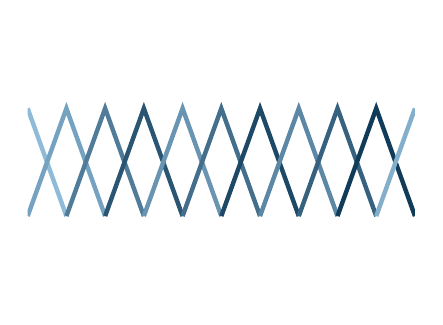
\begin{tikzpicture}
\begin{axis}[axis lines={none}, height={5cm}, width={6.5cm}, xmin={0}, xmax={1}, ymin={-0.75}, ymax={1.75}]
    \node at (0,-2.5) {};
    \node at (0,2.5) {};
    \node at (1,2.5) {};
    \node at (1,-2.5) {};
    \addplot[no markers, ultra thick, color={rgb,1:red,0.5608;green,0.7333;blue,0.851}]
        coordinates {
            (0.0,1)
            (0.1,0)
        }
        ;
    \addplot[no markers, ultra thick, color={rgb,1:red,0.4588;green,0.6353;blue,0.7529}]
        coordinates {
            (0.0,0)
            (0.1,1)
            (0.2,0)
        }
        ;
    \addplot[no markers, ultra thick, color={rgb,1:red,0.3137;green,0.4863;blue,0.6039}]
        coordinates {
            (0.1,0)
            (0.2,1)
            (0.3,0)
        }
        ;
    \addplot[no markers, ultra thick, color={rgb,1:red,0.1647;green,0.3333;blue,0.451}]
        coordinates {
            (0.2,0)
            (0.3,1)
            (0.4,0)
        }
        ;
    \addplot[no markers, ultra thick, color={rgb,1:red,0.4118;green,0.5843;blue,0.698}]
        coordinates {
            (0.3,0)
            (0.4,1)
            (0.5,0)
        }
        ;
    \addplot[no markers, ultra thick, color={rgb,1:red,0.2627;green,0.4353;blue,0.5529}]
        coordinates {
            (0.4,0)
            (0.5,1)
            (0.6,0)
        }
        ;
    \addplot[no markers, ultra thick, color={rgb,1:red,0.1137;green,0.2863;blue,0.4039}]
        coordinates {
            (0.5,0)
            (0.6,1)
            (0.7,0)
        }
        ;
    \addplot[no markers, ultra thick, color={rgb,1:red,0.3608;green,0.5333;blue,0.651}]
        coordinates {
            (0.6,0)
            (0.7,1)
            (0.8,0)
        }
        ;
    \addplot[no markers, ultra thick, color={rgb,1:red,0.2118;green,0.3843;blue,0.502}]
        coordinates {
            (0.7,0)
            (0.8,1)
            (0.9,0)
        }
        ;
    \addplot[no markers, ultra thick, color={rgb,1:red,0.0627;green,0.2353;blue,0.3529}]
        coordinates {
            (0.8,0)
            (0.9,1)
            (1.0,0)
        }
        ;
    \addplot[no markers, ultra thick, color={rgb,1:red,0.5137;green,0.6863;blue,0.8039}]
        coordinates {
            (0.9,0)
            (1.0,1)
        }
        ;
\end{axis}
\end{tikzpicture}
\end{document}

\caption{Finite element basis}
\end{subfigure}
\begin{subfigure}{0.49\textwidth}
\documentclass[tikz,11pt]{standalone}
\usepackage{lmodern}
\usepackage{pgfplots}
\pgfplotsset{compat=1.17}
\usepgfplotslibrary{external}
\usepgfplotslibrary{groupplots}
\usepgfplotslibrary{fillbetween}
\usetikzlibrary{fadings}
\begin{document}
\tikzsetnextfilename{gp-fe-samples}
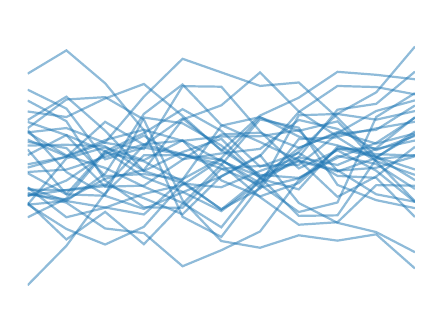
\begin{tikzpicture}
\begin{axis}[axis lines={none}, height={5cm}, width={6.5cm}, xmin={0}, xmax={1}, ymin={-1}, ymax={1}]
    \node at (0,-1) {};
    \node at (0,1) {};
    \node at (1,1) {};
    \node at (1,-1) {};
    \addplot[no markers, thick, color={rgb,1:red,0.1216;green,0.4667;blue,0.7059}, opacity={0.5}]
        coordinates {
            (0.0,0.09498494657968107)
            (0.1,-0.23724549096179692)
            (0.2,0.08397027095122997)
            (0.3,-0.10972245639341091)
            (0.4,-0.21968508478167026)
            (0.5,-0.362993432804414)
            (0.6,-0.14630627306008667)
            (0.7,0.07859285791045817)
            (0.8,0.36015447132830697)
            (0.9,0.519343540663884)
            (1.0,0.8594557360415592)
        }
        ;
    \addplot[no markers, thick, color={rgb,1:red,0.1216;green,0.4667;blue,0.7059}, opacity={0.5}]
        coordinates {
            (0.0,-0.248415646403542)
            (0.1,-0.20616224675591288)
            (0.2,-0.16498192859860078)
            (0.3,-0.26693344731055546)
            (0.4,-0.3867268766662556)
            (0.5,-0.10362872677302054)
            (0.6,0.052922753742921894)
            (0.7,-0.30269606285454553)
            (0.8,-0.4498755889085098)
            (0.9,-0.5190800520916447)
            (1.0,-0.6682400935611759)
        }
        ;
    \addplot[no markers, thick, color={rgb,1:red,0.1216;green,0.4667;blue,0.7059}, opacity={0.5}]
        coordinates {
            (0.0,-0.2503834790053334)
            (0.1,-0.1357982424464937)
            (0.2,0.05962972299014967)
            (0.3,0.19737315608634293)
            (0.4,0.02226238323326468)
            (0.5,0.06561816908182379)
            (0.6,0.09921618716025414)
            (0.7,0.31424319871836476)
            (0.8,0.2478699283715867)
            (0.9,0.09011380159014455)
            (1.0,0.19601176646981291)
        }
        ;
    \addplot[no markers, thick, color={rgb,1:red,0.1216;green,0.4667;blue,0.7059}, opacity={0.5}]
        coordinates {
            (0.0,0.1675636522896265)
            (0.1,0.044686517914202126)
            (0.2,0.16456864123017373)
            (0.3,0.2415537271589137)
            (0.4,0.15898629948033677)
            (0.5,0.19168500688446266)
            (0.6,0.1934583524376249)
            (0.7,0.2375948594525495)
            (0.8,-0.06254357898884245)
            (0.9,-0.0407783193449509)
            (1.0,0.04436298938955947)
        }
        ;
    \addplot[no markers, thick, color={rgb,1:red,0.1216;green,0.4667;blue,0.7059}, opacity={0.5}]
        coordinates {
            (0.0,-0.3144146222868028)
            (0.1,0.029021939558603736)
            (0.2,0.11028846705159012)
            (0.3,0.015260205660267923)
            (0.4,0.16334094237539304)
            (0.5,-0.13491260081592893)
            (0.6,-0.2534482129827321)
            (0.7,-0.1544372433880578)
            (0.8,0.10187356508243582)
            (0.9,0.03969323522136157)
            (1.0,-0.05384782455004117)
        }
        ;
    \addplot[no markers, thick, color={rgb,1:red,0.1216;green,0.4667;blue,0.7059}, opacity={0.5}]
        coordinates {
            (0.0,-0.2029673870337705)
            (0.1,-0.2084641100807012)
            (0.2,-0.17724297600776548)
            (0.3,0.12653203961388937)
            (0.4,0.3255608642606018)
            (0.5,0.09190811345779767)
            (0.6,-0.09370878858931794)
            (0.7,-0.11644900546724403)
            (0.8,0.04731483804083073)
            (0.9,-0.013179872163944568)
            (1.0,-0.19793103484408275)
        }
        ;
    \addplot[no markers, thick, color={rgb,1:red,0.1216;green,0.4667;blue,0.7059}, opacity={0.5}]
        coordinates {
            (0.0,0.05335483601076096)
            (0.1,0.20182410692842942)
            (0.2,0.08049120021244033)
            (0.3,0.2168329482410183)
            (0.4,0.394380450818598)
            (0.5,0.23281312455308287)
            (0.6,-0.032649803187476296)
            (0.7,0.06919889488388947)
            (0.8,-0.10139931507437297)
            (0.9,-0.11571474855862718)
            (1.0,-0.4070819093997374)
        }
        ;
    \addplot[no markers, thick, color={rgb,1:red,0.1216;green,0.4667;blue,0.7059}, opacity={0.5}]
        coordinates {
            (0.0,-0.08103014675922283)
            (0.1,-0.23819427341055302)
            (0.2,-0.24925658102255682)
            (0.3,-0.3468875436868798)
            (0.4,-0.22305363417614316)
            (0.5,-0.10639324803772734)
            (0.6,0.04610567994896077)
            (0.7,0.3733976038358125)
            (0.8,0.5667516590827262)
            (0.9,0.558853657225792)
            (1.0,0.5045670504911812)
        }
        ;
    \addplot[no markers, thick, color={rgb,1:red,0.1216;green,0.4667;blue,0.7059}, opacity={0.5}]
        coordinates {
            (0.0,-0.015287870137528574)
            (0.1,0.04044600177559839)
            (0.2,0.14728871228334015)
            (0.3,0.4867599911148241)
            (0.4,0.7687615874000627)
            (0.5,0.6677387866342814)
            (0.6,0.5670195127727382)
            (0.7,0.5926237591950586)
            (0.8,0.330409508896345)
            (0.9,0.03821543627130975)
            (1.0,0.20578071002528475)
        }
        ;
    \addplot[no markers, thick, color={rgb,1:red,0.1216;green,0.4667;blue,0.7059}, opacity={0.5}]
        coordinates {
            (0.0,0.3771739535675994)
            (0.1,0.3361186733995483)
            (0.2,0.4738092580676894)
            (0.3,0.5815526377541662)
            (0.4,0.3438719571947418)
            (0.5,0.08567649330498582)
            (0.6,0.34711708387174867)
            (0.7,0.4795447476045996)
            (0.8,0.6718479765942938)
            (0.9,0.6497304042503554)
            (1.0,0.6166449545717821)
        }
        ;
    \addplot[no markers, thick, color={rgb,1:red,0.1216;green,0.4667;blue,0.7059}, opacity={0.5}]
        coordinates {
            (0.0,-0.18985754587502562)
            (0.1,-0.2881463884810402)
            (0.2,-0.3358656835794836)
            (0.3,-0.3880663239703827)
            (0.4,-0.12930318492181092)
            (0.5,0.2717710718919262)
            (0.6,0.33580900112653106)
            (0.7,0.1906160837732082)
            (0.8,0.12497603016947674)
            (0.9,0.04114539860293693)
            (1.0,-0.1324974326581379)
        }
        ;
    \addplot[no markers, thick, color={rgb,1:red,0.1216;green,0.4667;blue,0.7059}, opacity={0.5}]
        coordinates {
            (0.0,-0.31532251381935683)
            (0.1,-0.2875905655516834)
            (0.2,-0.08491687616987913)
            (0.3,0.3590761423838963)
            (0.4,0.57818534614458)
            (0.5,0.27647405457604274)
            (0.6,0.15025030317262622)
            (0.7,0.014437922663342921)
            (0.8,-0.25730001753378323)
            (0.9,-0.10530039800722006)
            (1.0,0.11455050149477689)
        }
        ;
    \addplot[no markers, thick, color={rgb,1:red,0.1216;green,0.4667;blue,0.7059}, opacity={0.5}]
        coordinates {
            (0.0,0.22215315525793342)
            (0.1,0.2541812278284589)
            (0.2,0.14451523755741633)
            (0.3,0.09802297307842264)
            (0.4,0.5651538283335916)
            (0.5,0.5614156681057751)
            (0.6,0.23020025539141167)
            (0.7,-0.04574522285471535)
            (0.8,0.08849723498577654)
            (0.9,-0.06293972831062909)
            (1.0,-0.29585172819305144)
        }
        ;
    \addplot[no markers, thick, color={rgb,1:red,0.1216;green,0.4667;blue,0.7059}, opacity={0.5}]
        coordinates {
            (0.0,-0.30056056705031353)
            (0.1,-0.5735943105559179)
            (0.2,-0.3687449953381548)
            (0.3,-0.6086719325335511)
            (0.4,-0.30952402775207793)
            (0.5,-0.020128521282795155)
            (0.6,0.31815684751987083)
            (0.7,0.2570489701045229)
            (0.8,-0.16839634149790317)
            (0.9,-0.2816352177182484)
            (1.0,-0.3408799035928914)
        }
        ;
    \addplot[no markers, thick, color={rgb,1:red,0.1216;green,0.4667;blue,0.7059}, opacity={0.5}]
        coordinates {
            (0.0,-0.03972986920040689)
            (0.1,0.040706308702241234)
            (0.2,0.3002983680835113)
            (0.3,0.12953320889880968)
            (0.4,0.061814177616659347)
            (0.5,-0.047781726630583256)
            (0.6,-0.1665446575506989)
            (0.7,-0.36986713187245696)
            (0.8,-0.29861870688457715)
            (0.9,0.3363605491470263)
            (1.0,0.5135003222750159)
        }
        ;
    \addplot[no markers, thick, color={rgb,1:red,0.1216;green,0.4667;blue,0.7059}, opacity={0.5}]
        coordinates {
            (0.0,-0.18744044637220292)
            (0.1,-0.40880023266822296)
            (0.2,-0.33796905519283804)
            (0.3,-0.2346578450261016)
            (0.4,-0.16850971289521735)
            (0.5,0.022130983258210567)
            (0.6,-0.18861248563534636)
            (0.7,-0.11989353762631096)
            (0.8,0.033589427651770906)
            (0.9,0.14376476674326127)
            (1.0,0.3311631970792885)
        }
        ;
    \addplot[no markers, thick, color={rgb,1:red,0.1216;green,0.4667;blue,0.7059}, opacity={0.5}]
        coordinates {
            (0.0,0.3135726814837102)
            (0.1,0.48719897526008427)
            (0.2,0.2344228725045181)
            (0.3,-0.06507293182539431)
            (0.4,0.07597273314250681)
            (0.5,0.174013710021922)
            (0.6,-0.1097978199343743)
            (0.7,-0.3985024434977161)
            (0.8,-0.39441333862405137)
            (0.9,0.022687186136147345)
            (1.0,0.0527019344888005)
        }
        ;
    \addplot[no markers, thick, color={rgb,1:red,0.1216;green,0.4667;blue,0.7059}, opacity={0.5}]
        coordinates {
            (0.0,0.1512210038730948)
            (0.1,0.10533584944543142)
            (0.2,-0.18215451399242966)
            (0.3,-0.17345480128669077)
            (0.4,0.018910314323305265)
            (0.5,0.20653717824073642)
            (0.6,0.21979625077128945)
            (0.7,0.10804929779207927)
            (0.8,0.21648124030895982)
            (0.9,0.38101310152878126)
            (1.0,0.45982568237665306)
        }
        ;
    \addplot[no markers, thick, color={rgb,1:red,0.1216;green,0.4667;blue,0.7059}, opacity={0.5}]
        coordinates {
            (0.0,-0.3130528984608863)
            (0.1,-0.49590345770390504)
            (0.2,-0.6114476428074167)
            (0.3,-0.4794822059658766)
            (0.4,-0.15843376288247782)
            (0.5,-0.1855877652058837)
            (0.6,-0.06486190960282834)
            (0.7,0.03648192656615157)
            (0.8,-0.020323387522402463)
            (0.9,0.09870090798211413)
            (1.0,0.16147284791562025)
        }
        ;
    \addplot[no markers, thick, color={rgb,1:red,0.1216;green,0.4667;blue,0.7059}, opacity={0.5}]
        coordinates {
            (0.0,0.12384145516389294)
            (0.1,0.13008348679668214)
            (0.2,0.11808873323740614)
            (0.3,-0.06571654919329127)
            (0.4,-0.15299856843659684)
            (0.5,-0.34908933896556815)
            (0.6,-0.1962625402314788)
            (0.7,0.17214272347064358)
            (0.8,0.1852990731618942)
            (0.9,0.00829654173759608)
            (1.0,-0.09407634160639759)
        }
        ;
    \addplot[no markers, thick, color={rgb,1:red,0.1216;green,0.4667;blue,0.7059}, opacity={0.5}]
        coordinates {
            (0.0,0.45825834874853605)
            (0.1,0.30490962967818663)
            (0.2,-0.13597981482638574)
            (0.3,-0.3344120158291897)
            (0.4,-0.33870806904242406)
            (0.5,-0.0489434622481658)
            (0.6,-0.02661323308055348)
            (0.7,-0.019524227930935438)
            (0.8,0.21109011290271879)
            (0.9,0.24068722762025072)
            (1.0,0.42193197159052037)
        }
        ;
    \addplot[no markers, thick, color={rgb,1:red,0.1216;green,0.4667;blue,0.7059}, opacity={0.5}]
        coordinates {
            (0.0,-0.22725945283325516)
            (0.1,-0.30017083860654287)
            (0.2,-0.49194021101572094)
            (0.3,-0.5260130381174278)
            (0.4,-0.7727206322044063)
            (0.5,-0.6536016052402311)
            (0.6,-0.5144976615783261)
            (0.7,-0.13209850986824623)
            (0.8,0.09837456838852462)
            (0.9,0.10497326284694276)
            (1.0,0.3349548114302829)
        }
        ;
    \addplot[no markers, thick, color={rgb,1:red,0.1216;green,0.4667;blue,0.7059}, opacity={0.5}]
        coordinates {
            (0.0,0.6581864356183867)
            (0.1,0.8311198706787929)
            (0.2,0.5870303027865628)
            (0.3,0.2382071643974603)
            (0.4,-0.40569474134826355)
            (0.5,-0.5543182918145741)
            (0.6,-0.17843492154013396)
            (0.7,0.34921274681561976)
            (0.8,0.35872997129960943)
            (0.9,0.3164523864672074)
            (1.0,0.3803613779551002)
        }
        ;
    \addplot[no markers, thick, color={rgb,1:red,0.1216;green,0.4667;blue,0.7059}, opacity={0.5}]
        coordinates {
            (0.0,0.5389162073013769)
            (0.1,0.39846637871351187)
            (0.2,0.021717357631867624)
            (0.3,0.10976214872156453)
            (0.4,0.05571861796187734)
            (0.5,-0.016477646684562842)
            (0.6,-0.2589603342514648)
            (0.7,-0.46417425899577036)
            (0.8,-0.44558334163094604)
            (0.9,-0.1698896076582391)
            (1.0,-0.17396801070167223)
        }
        ;
    \addplot[no markers, thick, color={rgb,1:red,0.1216;green,0.4667;blue,0.7059}, opacity={0.5}]
        coordinates {
            (0.0,-0.4089524589298445)
            (0.1,-0.2688523219420219)
            (0.2,0.0734099541975586)
            (0.3,0.006709014058455922)
            (0.4,-0.14280126597013315)
            (0.5,-0.3516432645416361)
            (0.6,-0.11968972443715326)
            (0.7,0.10516211930499766)
            (0.8,0.22460682609870647)
            (0.9,0.13878622732829526)
            (1.0,0.21441533879341168)
        }
        ;
    \addplot[no markers, thick, color={rgb,1:red,0.1216;green,0.4667;blue,0.7059}, opacity={0.5}]
        coordinates {
            (0.0,0.2218607015708971)
            (0.1,0.050503263220838396)
            (0.2,-0.042112737901707935)
            (0.3,-0.18117675025100122)
            (0.4,-0.30222276265720455)
            (0.5,-0.48332563910544935)
            (0.6,-0.12182894902118528)
            (0.7,-0.20157343544005407)
            (0.8,0.11615776353326586)
            (0.9,0.06012711389721035)
            (1.0,0.0497329882211008)
        }
        ;
    \addplot[no markers, thick, color={rgb,1:red,0.1216;green,0.4667;blue,0.7059}, opacity={0.5}]
        coordinates {
            (0.0,0.29959093038775864)
            (0.1,0.20101230127873745)
            (0.2,-0.10298775191572299)
            (0.3,-0.08767324836108821)
            (0.4,-0.12569098946548252)
            (0.5,0.030898977318924704)
            (0.6,0.3329179678439075)
            (0.7,0.23327614739336047)
            (0.8,0.303698476639959)
            (0.9,0.008057624712880322)
            (1.0,-0.2898670721574453)
        }
        ;
    \addplot[no markers, thick, color={rgb,1:red,0.1216;green,0.4667;blue,0.7059}, opacity={0.5}]
        coordinates {
            (0.0,-0.9134460180956976)
            (0.1,-0.6208565348905857)
            (0.2,-0.22991800931285852)
            (0.3,0.05174190397439881)
            (0.4,0.053556703311603844)
            (0.5,0.01801386768371227)
            (0.6,-0.15577423841366916)
            (0.7,0.03811206536840217)
            (0.8,0.3907979532263721)
            (0.9,0.4340000907314427)
            (1.0,0.6731635853975865)
        }
        ;
    \addplot[no markers, thick, color={rgb,1:red,0.1216;green,0.4667;blue,0.7059}, opacity={0.5}]
        coordinates {
            (0.0,0.25298667677015)
            (0.1,0.46642172194134024)
            (0.2,0.48390431268903084)
            (0.3,0.3173754124862537)
            (0.4,-0.28327097061151457)
            (0.5,-0.5855244751048659)
            (0.6,-0.6351947442760961)
            (0.7,-0.5428122365582818)
            (0.8,-0.582476558681603)
            (0.9,-0.5355741032474847)
            (1.0,-0.7890378646081362)
        }
        ;
    \addplot[no markers, thick, color={rgb,1:red,0.1216;green,0.4667;blue,0.7059}, opacity={0.5}]
        coordinates {
            (0.0,-0.07238852246387674)
            (0.1,-0.054583482079260316)
            (0.2,0.04003771784706045)
            (0.3,0.1338923994859722)
            (0.4,0.16047348454689142)
            (0.5,0.00875571571155339)
            (0.6,-0.10617525122315012)
            (0.7,0.01488893371267623)
            (0.8,-0.05905015534383126)
            (0.9,-0.23798135072484627)
            (1.0,-0.2938438180906397)
        }
        ;
    \addplot[no markers, thick, color={rgb,1:red,0.1216;green,0.4667;blue,0.7059}, opacity={0.5}]
        coordinates {
            (0.0,-0.23829198262372392)
            (0.1,-0.2760910164953669)
            (0.2,-0.12286562931116876)
            (0.3,-0.05811129033880735)
            (0.4,0.31780877910135175)
            (0.5,0.4228334623508409)
            (0.6,0.667300297902088)
            (0.7,0.3774818415253705)
            (0.8,0.19114581802895492)
            (0.9,0.2519372739520995)
            (1.0,0.30081626107424186)
        }
        ;
    \addplot[no markers, thick, color={rgb,1:red,0.1216;green,0.4667;blue,0.7059}, opacity={0.5}]
        coordinates {
            (0.0,0.23982650256559315)
            (0.1,-0.0729274722427919)
            (0.2,-0.2429224333538238)
            (0.3,0.3323647380451614)
            (0.4,0.2894497106128856)
            (0.5,0.12443603525229363)
            (0.6,-0.11974226680923587)
            (0.7,0.007756602789161979)
            (0.8,-0.06842572606557594)
            (0.9,0.031731320414588975)
            (1.0,0.22923136369299327)
        }
        ;
\end{axis}
\end{tikzpicture}
\end{document}

\caption{Approximate prior samples}
\end{subfigure}
\caption{Illustration of finite element approximate prior samples for a Matérn kernel with smoothness $3/2$ and length scale $\kappa$.
In one dimension, following \textcite{lindgren11}, the bilinear form for this kernel is $a(f,h) = \int_X \frac{3}{\kappa^2} f(x)h(x) + \grad f(x) \. \grad h(x) \d x$. 
Since this bilinear form is of first order in both arguments, we employ a piecewise linear finite element basis consisting of compactly supported triangle-shaped functions, using it to represent both $f$ and $h$.
This results in matrices $\m{A}$ and $\m{M}$ which are symmetric tridiagonal.}
\label{fig:gp-fe-prior}
\end{figure}

The main difficulty with finite element methods is that they typically demand more from practitioners compared to alternatives.
In particular, one usually needs to understand the stochastic partial differential equations governing the Gaussian process of interest with a reasonable degree of detail to know how to choose basis functions well.
Additionally, sparse linear algebra in a parallel environment with automatic differentiation can be cumbersome.

This concludes our presentation of techniques for constructing approximate priors.
In general, the best choice for a particular application will depend on the detailed requirements of the situation.
We now proceed to study other aspects of the pathwise viewpoint.

\section{Approximating pathwise data-dependent terms}

In the preceding section, we discussed techniques for approximating the prior using a finite set of basis functions with random coefficients.
Such approximations enabled us to construct approximate pathwise representations of posterior Gaussian processes with $\c{O}(n_*)$ computational complexity, where we recall again that $n_*$ is the number of points where we wish to evaluate the posterior at.
We now consider the other computational costs in the formula: $\c{O}(n^3)$, where $n$ is the size of the training data.
These arise because computing
\[
(f \given\v{y})(\omega,\v\gamma) \overset{\d}{=} f(\omega,\.) + \m{K}_{(\.)\v{x}} (\m{K}_{\v{x}\v{x}} + \m\Sigma)^{-1}(\v\gamma - \v{f}(\omega) - \v\eps(\omega))
\]
requires us to invert an $n\x n$ matrix.
We now ask: from a pathwise perspective, what techniques are available for reducing these costs?

\subsection{Inducing points}

Consider a simple approach to reducing the above cubic costs: instead of conditioning the Gaussian process on the full set of values $(x_1,y_1),..,(x_n,y_n)$, find a different data set $(z_1,\mu_1),..,(z_m,\mu_m)$, for which $m \ll  n$ and yet the posterior is approximately the same.
To ensure this approximation is expressive enough, we can either (i) make $\v\mu$ random with a learnable mean and covariance, or (ii) introduce a learned noise covariance $\m\Lambda$, rather than reusing the one from the original model.
The latter gives
\[
(f \given\v{u})(\omega,\v\mu) = f(\omega,\.) + \m{K}_{(\.)\v{z}} (\m{K}_{\v{z}\v{z}} + \m\Lambda)^{-1}(\v\mu - \v{f}(\omega) - \v\epsilon(\omega))
\]
where $f\given\v{u}$ is the posterior under the modified likelihood employing the noise covariance $\m\Lambda$.
This approximation has a particularly simple interpretation: we can re-write it as
\[
(f \given\v{u})(\omega,\v\mu) = f(\omega,\.) + \sum_{j=1}^m v_j(\omega) k(z_j,\.)
\]
where $\v{v}(\omega) = (\m{K}_{\v{z}\v{z}} + \m\Lambda)^{-1}(\v\mu - \v{f}(\omega) - \v\epsilon(\omega))$.
Thus, we see that all we have done is replaced a large sum of data-dependent functions $k(x_j,\.)$ with $j=1,..,n$ induced by the kernel with a much smaller sum involving a sparsified set of functions $k(z_j,\.)$ with $j=1,..,m$ and $m \ll n$.

Given such an approximate posterior, how should we select the introduced hyperparameters $\v{z},\v\mu,\m\Lambda$ to ensure quality?
At minimum, we should attempt to guarantee consistency of the approximation, in the sense that if $m = n$ then one can choose $\v{z} = \v{x}$, $\v\mu = \v\gamma$, and $\m\Lambda = \m\Sigma$ to recover the desired posterior.
We therefore seek to minimize some notion of \emph{distance} on the space of probability measures.

The most natural choice one can consider is arguably the one that emerged from the analysis of Bayes' Rule presented in \Cref{ch:intro}: namely, the \emph{Kullback--Leibler divergence}.
Minimizing this amounts to replacing the measure space in the variational formulation of Bayes' Rule of \Cref{prop:variational-bayes} with the parameterized subspace of measures induced by the set of approximate posteriors with different parameter values, which we the \emph{variational family}.
This yields the optimization problem 
\[
\argmin_{\bb{q}_f\in\bb{Q}} D_{\f{KL}}(\bb{q}_f \from \pi_f) + \frac{1}{2}\operatorname*{\E}_{f\~\bb{q}_f} (\v\gamma - f(\v{x}))^T \m\Sigma^{-1} (\v\gamma - f(\v{x}))
\]
where $\bb{Q}$ is the set of all measures equal to the distribution of $f\given\v{u}$ for some choice of variational parameter values $\v{z},\v\mu,\m\Lambda$, and $\bb{q}_f$ is the distribution of $f\given\v{u}$ for a specific set of such values.
Note that we have dropped constant terms from the likelihood density because they do not affect the optima.
Our \emph{variational approximation} is obtained by solving this optimization problem, which it turns out is necessarily well-posed.

\begin{proposition}[Variational objective for inducing point approximations]
For all $\v{x},\v{y},\m\Sigma$, and all $\v{z},\v\mu,\m\Lambda$, the Kullback--Leibler divergence $D_{\f{KL}}(\bb{q}_f \from \pi_{f \given\v{y}})$ is finite and equal to the above objective up to an additive constant.
Moreover, the prior Kullback--Leibler divergence $D_{\f{KL}}(\bb{q}_f \from \pi_f) = D_{\f{KL}}(\bb{q}_{f(\v{z})} \from \pi_{f(\v{z})})$ reduces to the Kullback--Leibler divergence between the respective finite-dimensional marginal distributions at the inducing locations $\v{z}$.
\end{proposition}

\begin{proof}
We consider the two terms in the objective and the additive constant.
\1 Finiteness of the first term, along with the second claim, follows by the chain rule for Kullback--Leibler divergences, since $\bb{q}_f$ is by construction a conditional distribution of a Gaussian process with the same covariance kernel as $k$.
\2 Finiteness of the second term follows immediately, because it is the expectation of a quadratic with respect to a multivariate Gaussian.
\3 Finiteness of the additive constant also follows, because it is by definition the log-density of a multivariate Gaussian.
\0 
The claim follows. 
\end{proof}

We have therefore proven that the \emph{inducing point} approximation of \textcite{opper09}, when re-interpreted using the variational inference framework of \textcite{titsias09}, coincides with the pathwise variational approximation constructed here.
The same is true for other classes of inducing points, including the family where $\v{u}$ is randomized, as originally proposed by \textcite{titsias09}.

\begin{figure}
\begin{subfigure}{\textwidth}
\documentclass[tikz,11pt]{standalone}
\usepackage{lmodern}
\usepackage{pgfplots}
\pgfplotsset{compat=1.17}
\usepgfplotslibrary{external}
\usepgfplotslibrary{groupplots}
\usepgfplotslibrary{fillbetween}
\usetikzlibrary{fadings}
\begin{document}
\tikzsetnextfilename{gp-ip-cond}
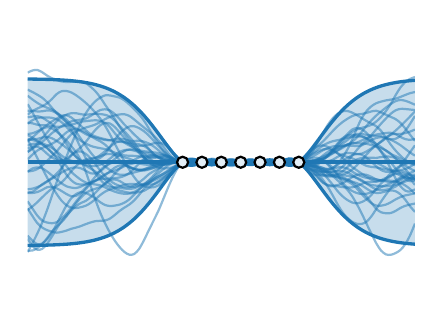
\begin{tikzpicture}
\begin{axis}[axis lines={none}, height={5cm}, width={6.5cm}, xmin={0}, xmax={1}, ymin={-1}, ymax={1}]
    \node at (0,-1) {};
    \node at (0,1) {};
    \node at (1,1) {};
    \node at (1,-1) {};
    \addplot[no markers, smooth, very thick, color={rgb,1:red,0.1216;green,0.4667;blue,0.7059}, name path={upper}]
        coordinates {
            (0.0,0.6183759001569293)
            (0.0125,0.6179414132292164)
            (0.025,0.6173818196504973)
            (0.0375,0.6166636264786727)
            (0.05,0.6157452847723878)
            (0.0625,0.6145755705112692)
            (0.075,0.6130917492583698)
            (0.0875,0.611217534152527)
            (0.1,0.6088608643958772)
            (0.1125,0.6059115550619001)
            (0.125,0.6022388998513882)
            (0.1375,0.5976893474366167)
            (0.15,0.5920844203114609)
            (0.1625,0.5852191036206689)
            (0.175,0.5768610012126524)
            (0.1875,0.5667506379406325)
            (0.2,0.554603381535063)
            (0.2125,0.5401135641325681)
            (0.225,0.5229615016567215)
            (0.2375,0.5028242356698059)
            (0.25,0.47939095070793525)
            (0.2625,0.4523841386119978)
            (0.275,0.4215876691322361)
            (0.2875,0.38688294785992566)
            (0.3,0.34829424002549675)
            (0.3125,0.3060439165901728)
            (0.325,0.2606176819930551)
            (0.3375,0.21283851703519807)
            (0.35,0.16394570096414363)
            (0.3625,0.11567121175298584)
            (0.375,0.07029933664714681)
            (0.3875,0.030691219283322323)
            (0.4,0.0019598599626162306)
            (0.4125,0.01817551199281946)
            (0.425,0.02228449016297733)
            (0.4375,0.014500946338491793)
            (0.45,0.0019593682151072666)
            (0.4625,0.013051680839442194)
            (0.475,0.01779838385597123)
            (0.4875,0.012511954830900717)
            (0.5,0.0019590537211104293)
            (0.5125,0.01227709781136154)
            (0.525,0.017091469939936512)
            (0.5375,0.012201043059064918)
            (0.55,0.001958988018003537)
            (0.5625,0.012201043059071472)
            (0.575,0.017091469939970825)
            (0.5875,0.012277097811480958)
            (0.6,0.001959053721096823)
            (0.6125,0.012511954830892194)
            (0.625,0.017798383855959245)
            (0.6375,0.013051680839452406)
            (0.65,0.0019593682151072666)
            (0.6625,0.014500946338416424)
            (0.675,0.02228449016288044)
            (0.6875,0.018175511992773993)
            (0.7,0.0019598599626162306)
            (0.7125,0.030691219283303213)
            (0.725,0.07029933664715023)
            (0.7375,0.11567121175299483)
            (0.75,0.1639457009641521)
            (0.7625,0.21283851703519294)
            (0.775,0.26061768199304913)
            (0.7875,0.30604391659016444)
            (0.8,0.34829424002549164)
            (0.8125,0.38688294785991467)
            (0.825,0.42158766913223117)
            (0.8375,0.45238413861199117)
            (0.85,0.4793909507079325)
            (0.8625,0.5028242356698016)
            (0.875,0.5229615016567181)
            (0.8875,0.540113564132565)
            (0.9,0.5546033815350607)
            (0.9125,0.5667506379406303)
            (0.925,0.5768610012126504)
            (0.9375,0.5852191036206674)
            (0.95,0.5920844203114596)
            (0.9625,0.597689347436616)
            (0.975,0.6022388998513876)
            (0.9875,0.6059115550618993)
            (1.0,0.6088608643958766)
        }
        ;
    \addplot[no markers, smooth, very thick, color={rgb,1:red,0.1216;green,0.4667;blue,0.7059}, name path={lower}]
        coordinates {
            (0.0,-0.6183759001569293)
            (0.0125,-0.6179414132292164)
            (0.025,-0.6173818196504973)
            (0.0375,-0.6166636264786727)
            (0.05,-0.6157452847723878)
            (0.0625,-0.6145755705112692)
            (0.075,-0.6130917492583698)
            (0.0875,-0.611217534152527)
            (0.1,-0.6088608643958772)
            (0.1125,-0.6059115550619001)
            (0.125,-0.6022388998513882)
            (0.1375,-0.5976893474366167)
            (0.15,-0.5920844203114609)
            (0.1625,-0.5852191036206689)
            (0.175,-0.5768610012126524)
            (0.1875,-0.5667506379406325)
            (0.2,-0.554603381535063)
            (0.2125,-0.5401135641325681)
            (0.225,-0.5229615016567215)
            (0.2375,-0.5028242356698059)
            (0.25,-0.47939095070793525)
            (0.2625,-0.4523841386119978)
            (0.275,-0.4215876691322361)
            (0.2875,-0.38688294785992566)
            (0.3,-0.34829424002549675)
            (0.3125,-0.3060439165901728)
            (0.325,-0.2606176819930551)
            (0.3375,-0.21283851703519807)
            (0.35,-0.16394570096414363)
            (0.3625,-0.11567121175298584)
            (0.375,-0.07029933664714681)
            (0.3875,-0.030691219283322323)
            (0.4,-0.0019598599626162306)
            (0.4125,-0.01817551199281946)
            (0.425,-0.02228449016297733)
            (0.4375,-0.014500946338491793)
            (0.45,-0.0019593682151072666)
            (0.4625,-0.013051680839442194)
            (0.475,-0.01779838385597123)
            (0.4875,-0.012511954830900717)
            (0.5,-0.0019590537211104293)
            (0.5125,-0.01227709781136154)
            (0.525,-0.017091469939936512)
            (0.5375,-0.012201043059064918)
            (0.55,-0.001958988018003537)
            (0.5625,-0.012201043059071472)
            (0.575,-0.017091469939970825)
            (0.5875,-0.012277097811480958)
            (0.6,-0.001959053721096823)
            (0.6125,-0.012511954830892194)
            (0.625,-0.017798383855959245)
            (0.6375,-0.013051680839452406)
            (0.65,-0.0019593682151072666)
            (0.6625,-0.014500946338416424)
            (0.675,-0.02228449016288044)
            (0.6875,-0.018175511992773993)
            (0.7,-0.0019598599626162306)
            (0.7125,-0.030691219283303213)
            (0.725,-0.07029933664715023)
            (0.7375,-0.11567121175299483)
            (0.75,-0.1639457009641521)
            (0.7625,-0.21283851703519294)
            (0.775,-0.26061768199304913)
            (0.7875,-0.30604391659016444)
            (0.8,-0.34829424002549164)
            (0.8125,-0.38688294785991467)
            (0.825,-0.42158766913223117)
            (0.8375,-0.45238413861199117)
            (0.85,-0.4793909507079325)
            (0.8625,-0.5028242356698016)
            (0.875,-0.5229615016567181)
            (0.8875,-0.540113564132565)
            (0.9,-0.5546033815350607)
            (0.9125,-0.5667506379406303)
            (0.925,-0.5768610012126504)
            (0.9375,-0.5852191036206674)
            (0.95,-0.5920844203114596)
            (0.9625,-0.597689347436616)
            (0.975,-0.6022388998513876)
            (0.9875,-0.6059115550618993)
            (1.0,-0.6088608643958766)
        }
        ;
    \addplot[color={rgb,1:red,0.1216;green,0.4667;blue,0.7059}, opacity={0.25}]
        fill between [of = upper and lower]
        ;
    \addplot[no markers, smooth, ultra thick, color={rgb,1:red,0.1216;green,0.4667;blue,0.7059}]
        coordinates {
            (0.0,0.0)
            (0.0125,0.0)
            (0.025,0.0)
            (0.0375,0.0)
            (0.05,0.0)
            (0.0625,0.0)
            (0.075,0.0)
            (0.0875,0.0)
            (0.1,0.0)
            (0.1125,0.0)
            (0.125,0.0)
            (0.1375,0.0)
            (0.15,0.0)
            (0.1625,0.0)
            (0.175,0.0)
            (0.1875,0.0)
            (0.2,0.0)
            (0.2125,0.0)
            (0.225,0.0)
            (0.2375,0.0)
            (0.25,0.0)
            (0.2625,0.0)
            (0.275,0.0)
            (0.2875,0.0)
            (0.3,0.0)
            (0.3125,0.0)
            (0.325,0.0)
            (0.3375,0.0)
            (0.35,0.0)
            (0.3625,0.0)
            (0.375,0.0)
            (0.3875,0.0)
            (0.4,0.0)
            (0.4125,0.0)
            (0.425,0.0)
            (0.4375,0.0)
            (0.45,0.0)
            (0.4625,0.0)
            (0.475,0.0)
            (0.4875,0.0)
            (0.5,0.0)
            (0.5125,0.0)
            (0.525,0.0)
            (0.5375,0.0)
            (0.55,0.0)
            (0.5625,0.0)
            (0.575,0.0)
            (0.5875,0.0)
            (0.6,0.0)
            (0.6125,0.0)
            (0.625,0.0)
            (0.6375,0.0)
            (0.65,0.0)
            (0.6625,0.0)
            (0.675,0.0)
            (0.6875,0.0)
            (0.7,0.0)
            (0.7125,0.0)
            (0.725,0.0)
            (0.7375,0.0)
            (0.75,0.0)
            (0.7625,0.0)
            (0.775,0.0)
            (0.7875,0.0)
            (0.8,0.0)
            (0.8125,0.0)
            (0.825,0.0)
            (0.8375,0.0)
            (0.85,0.0)
            (0.8625,0.0)
            (0.875,0.0)
            (0.8875,0.0)
            (0.9,0.0)
            (0.9125,0.0)
            (0.925,0.0)
            (0.9375,0.0)
            (0.95,0.0)
            (0.9625,0.0)
            (0.975,0.0)
            (0.9875,0.0)
            (1.0,0.0)
        }
        ;
    \addplot[no markers, smooth, thick, color={rgb,1:red,0.1216;green,0.4667;blue,0.7059}, opacity={0.5}]
        coordinates {
            (0.0,-0.567416763454854)
            (0.0125,-0.6239345603469724)
            (0.025,-0.6497111395348748)
            (0.0375,-0.6434749787395337)
            (0.05,-0.6065882699193706)
            (0.0625,-0.5528149758840583)
            (0.075,-0.49231697283469256)
            (0.0875,-0.4367326384236845)
            (0.1,-0.3960853573814609)
            (0.1125,-0.35928675933606313)
            (0.125,-0.32590007884666855)
            (0.1375,-0.3027099078295736)
            (0.15,-0.28679342036300104)
            (0.1625,-0.25951750695334863)
            (0.175,-0.22609422971794135)
            (0.1875,-0.19015268336199673)
            (0.2,-0.15632356321783128)
            (0.2125,-0.13367662855702167)
            (0.225,-0.12782901551817888)
            (0.2375,-0.13938317906111275)
            (0.25,-0.1614655410784847)
            (0.2625,-0.17956022636191166)
            (0.275,-0.18285877338353895)
            (0.2875,-0.17345777712196794)
            (0.3,-0.1642656767409213)
            (0.3125,-0.15161671880941205)
            (0.325,-0.1284860623873618)
            (0.3375,-0.105363691799612)
            (0.35,-0.08481208122807415)
            (0.3625,-0.06101375800061065)
            (0.375,-0.03737191139281315)
            (0.3875,-0.015734930426770655)
            (0.4,0.0005480191428804959)
            (0.4125,0.003483156063865067)
            (0.425,-0.0027996264665541837)
            (0.4375,-0.007540709162027093)
            (0.45,-0.0012856865092595315)
            (0.4625,0.007569005376226845)
            (0.475,0.010710171574062066)
            (0.4875,0.008461096663407774)
            (0.5,0.001279543937929395)
            (0.5125,-0.0027439427080779843)
            (0.525,-0.002270636342513843)
            (0.5375,-0.00026931177412264917)
            (0.55,-0.00050329501069446)
            (0.5625,-0.003007062531517002)
            (0.575,-0.005781192933225654)
            (0.5875,-0.001687006076737968)
            (0.6,-0.000366402896874396)
            (0.6125,-0.0015234834625640348)
            (0.625,0.0003880126958333424)
            (0.6375,-0.00023995748227063473)
            (0.65,0.0006347110672493758)
            (0.6625,0.01311176500625362)
            (0.675,0.02304993363193506)
            (0.6875,0.01758865600002775)
            (0.7,-0.00028709746757443755)
            (0.7125,-0.023891457583928105)
            (0.725,-0.04416333067687604)
            (0.7375,-0.05798757407973853)
            (0.75,-0.06031979137569464)
            (0.7625,-0.06551513301608006)
            (0.775,-0.08078706104230292)
            (0.7875,-0.10247014038273541)
            (0.8,-0.13363040798370218)
            (0.8125,-0.1674379419411004)
            (0.825,-0.2027954384277631)
            (0.8375,-0.25067723703248157)
            (0.85,-0.3118300223400434)
            (0.8625,-0.380367758937979)
            (0.875,-0.45695501875877886)
            (0.8875,-0.5309270006404374)
            (0.9,-0.6016251591189379)
            (0.9125,-0.6560182918756919)
            (0.925,-0.684633832455124)
            (0.9375,-0.6877338985052753)
            (0.95,-0.674562345162753)
            (0.9625,-0.6519545996843238)
            (0.975,-0.6083981392755548)
            (0.9875,-0.5423526036034301)
            (1.0,-0.4557556184182083)
        }
        ;
    \addplot[no markers, smooth, thick, color={rgb,1:red,0.1216;green,0.4667;blue,0.7059}, opacity={0.5}]
        coordinates {
            (0.0,0.021146825083518256)
            (0.0125,0.05705158637359092)
            (0.025,0.08674250891924434)
            (0.0375,0.10603760057068362)
            (0.05,0.12125374769485042)
            (0.0625,0.1372301400118982)
            (0.075,0.15842789550754294)
            (0.0875,0.1890412288080321)
            (0.1,0.22154697993083364)
            (0.1125,0.24151400845324822)
            (0.125,0.24522354651806635)
            (0.1375,0.23032777759836187)
            (0.15,0.20870977139091912)
            (0.1625,0.1936292003651922)
            (0.175,0.18371483957332418)
            (0.1875,0.1733466926119098)
            (0.2,0.16493473234621137)
            (0.2125,0.1644145467751616)
            (0.225,0.17224676362656027)
            (0.2375,0.17516724918614393)
            (0.25,0.17053611811013422)
            (0.2625,0.16022681913969103)
            (0.275,0.1584074870935224)
            (0.2875,0.1593898814491379)
            (0.3,0.1534635692293058)
            (0.3125,0.13986157244452355)
            (0.325,0.11860221279390451)
            (0.3375,0.08988262250704845)
            (0.35,0.059327943877424905)
            (0.3625,0.0318248962654826)
            (0.375,0.012693274705109031)
            (0.3875,0.00500390913855317)
            (0.4,-0.00016402265534834481)
            (0.4125,-6.035633734029211e-5)
            (0.425,-0.0007917516716441919)
            (0.4375,-0.002470159504335717)
            (0.45,0.0004659361741645683)
            (0.4625,0.00749127446046699)
            (0.475,0.010403583754570296)
            (0.4875,0.004797016658300762)
            (0.5,-0.0007444943006974514)
            (0.5125,-0.006063256938273781)
            (0.525,-0.010324718776740599)
            (0.5375,-0.007192831040584879)
            (0.55,0.0009254963647807868)
            (0.5625,0.007491725759329437)
            (0.575,0.005849358592207254)
            (0.5875,0.0009835943793931046)
            (0.6,-0.0009176632585710665)
            (0.6125,-0.0037310737983273223)
            (0.625,-0.003405138213642578)
            (0.6375,-0.0012955577936694107)
            (0.65,0.0006468624186165561)
            (0.6625,0.004618308220793732)
            (0.675,0.008625538560273371)
            (0.6875,0.008988981953997444)
            (0.7,-0.00023742662491677002)
            (0.7125,-0.020745405703244457)
            (0.725,-0.046700771565505894)
            (0.7375,-0.07813272317101339)
            (0.75,-0.11809147745349946)
            (0.7625,-0.1523107891423432)
            (0.775,-0.16821290321136084)
            (0.7875,-0.17283280626701603)
            (0.8,-0.1695923551652575)
            (0.8125,-0.1568269793386206)
            (0.825,-0.13622499052849973)
            (0.8375,-0.11088749940638615)
            (0.85,-0.09323246264463769)
            (0.8625,-0.08991872267266049)
            (0.875,-0.09344950902137689)
            (0.8875,-0.10875943045926023)
            (0.9,-0.1271851608328189)
            (0.9125,-0.13579965713675876)
            (0.925,-0.14218822443960927)
            (0.9375,-0.14742901570591765)
            (0.95,-0.14773576060240232)
            (0.9625,-0.13309134600512657)
            (0.975,-0.10767866357687375)
            (0.9875,-0.09292862024979152)
            (1.0,-0.09276776541391259)
        }
        ;
    \addplot[no markers, smooth, thick, color={rgb,1:red,0.1216;green,0.4667;blue,0.7059}, opacity={0.5}]
        coordinates {
            (0.0,0.4318197248408526)
            (0.0125,0.36978363228785116)
            (0.025,0.3031627110711796)
            (0.0375,0.2384962452975627)
            (0.05,0.17553008091978176)
            (0.0625,0.12240911081083423)
            (0.075,0.07230647285277371)
            (0.0875,0.022405200789459637)
            (0.1,-0.028298998138959905)
            (0.1125,-0.07108738159035904)
            (0.125,-0.10304782941301618)
            (0.1375,-0.1303673185980869)
            (0.15,-0.15031591901322436)
            (0.1625,-0.15961104269357343)
            (0.175,-0.1652555649705163)
            (0.1875,-0.17189478275898545)
            (0.2,-0.18639911103046003)
            (0.2125,-0.20446468024173117)
            (0.225,-0.21845911617683794)
            (0.2375,-0.22905702479914286)
            (0.25,-0.23441283854320905)
            (0.2625,-0.23267199383114734)
            (0.275,-0.2271382715682392)
            (0.2875,-0.22181598370546635)
            (0.3,-0.21270360206745786)
            (0.3125,-0.1911271916563958)
            (0.325,-0.16313471729900486)
            (0.3375,-0.14099345949182213)
            (0.35,-0.11813401150408127)
            (0.3625,-0.08794307745247067)
            (0.375,-0.053355130323804345)
            (0.3875,-0.017915531700170684)
            (0.4,-5.1162675154522996e-5)
            (0.4125,0.0011373649257249915)
            (0.425,-0.002719520562145432)
            (0.4375,-0.0037133031373685482)
            (0.45,9.688318194200213e-5)
            (0.4625,0.009138732600297142)
            (0.475,0.010232743463936239)
            (0.4875,0.004728098740919451)
            (0.5,-0.00011679361424948853)
            (0.5125,-0.0028345479579173494)
            (0.525,-0.008873624681472597)
            (0.5375,-0.0071557516531308984)
            (0.55,0.00012657135189925173)
            (0.5625,-0.0012311802798380123)
            (0.575,0.000457156392689409)
            (0.5875,0.002702448688678697)
            (0.6,-6.0983678814231085e-5)
            (0.6125,-0.0021979586160580655)
            (0.625,-0.0037496870140979466)
            (0.6375,-0.0022063112349804126)
            (0.65,-4.253983377072723e-5)
            (0.6625,-0.002938667247181337)
            (0.675,-0.004538687613300965)
            (0.6875,-0.005443685036772242)
            (0.7,4.8070444385546474e-5)
            (0.7125,0.004481221610894707)
            (0.725,0.008659129735333096)
            (0.7375,0.015377451596807902)
            (0.75,0.01832422573512414)
            (0.7625,0.024848208681593195)
            (0.775,0.04573403073016108)
            (0.7875,0.07772411438403244)
            (0.8,0.11547239477171764)
            (0.8125,0.15465575973777032)
            (0.825,0.19300173471241033)
            (0.8375,0.22461922812747492)
            (0.85,0.24347219807698953)
            (0.8625,0.2556811505152635)
            (0.875,0.2650233854570351)
            (0.8875,0.27804147796702283)
            (0.9,0.3025488146602333)
            (0.9125,0.3366967082791774)
            (0.925,0.379483656517342)
            (0.9375,0.4329937566670438)
            (0.95,0.4981360644635306)
            (0.9625,0.5550433117423488)
            (0.975,0.5953880109835706)
            (0.9875,0.6197086252626132)
            (1.0,0.6331147870255266)
        }
        ;
    \addplot[no markers, smooth, thick, color={rgb,1:red,0.1216;green,0.4667;blue,0.7059}, opacity={0.5}]
        coordinates {
            (0.0,-0.28989206819743785)
            (0.0125,-0.34443266857350047)
            (0.025,-0.3965185544694963)
            (0.0375,-0.43329718097282466)
            (0.05,-0.44773773938332556)
            (0.0625,-0.45302179228901474)
            (0.075,-0.4452078158791858)
            (0.0875,-0.41656322964300474)
            (0.1,-0.38198494314492215)
            (0.1125,-0.3392571308309781)
            (0.125,-0.2919191930021993)
            (0.1375,-0.24611328487642023)
            (0.15,-0.1993240823296902)
            (0.1625,-0.1616875870469099)
            (0.175,-0.1385546246060613)
            (0.1875,-0.11263558004879792)
            (0.2,-0.0884956851501233)
            (0.2125,-0.07396994653500018)
            (0.225,-0.061469830669160216)
            (0.2375,-0.04654891167607332)
            (0.25,-0.029607056575978993)
            (0.2625,-0.015597016978098795)
            (0.275,-0.006850762941538434)
            (0.2875,0.003532257461740587)
            (0.3,0.015326525487079301)
            (0.3125,0.026661839076111735)
            (0.325,0.03193608495232833)
            (0.3375,0.037166878405596265)
            (0.35,0.0440956191857837)
            (0.3625,0.04154130090935912)
            (0.375,0.02652907981118041)
            (0.3875,0.00790508091200548)
            (0.4,-0.00016992365555718036)
            (0.4125,0.002276523582005696)
            (0.425,0.002437269130831421)
            (0.4375,0.0008276576577480599)
            (0.45,0.0004223993373235202)
            (0.4625,-0.000954923353813697)
            (0.475,0.00029231009549768316)
            (0.4875,0.0007092678274729924)
            (0.5,-0.000533010108133336)
            (0.5125,0.0032879482004855576)
            (0.525,0.004893533711543996)
            (0.5375,0.0033682664780820826)
            (0.55,0.0004877277067255048)
            (0.5625,-0.0024712199430436677)
            (0.575,-0.0012747453513220486)
            (0.5875,0.00119987350820433)
            (0.6,-0.0004290594181808882)
            (0.6125,-0.005464515754157184)
            (0.625,-0.005061906477249856)
            (0.6375,0.0005874730707819964)
            (0.65,0.00037076348001385817)
            (0.6625,-0.003292814500227448)
            (0.675,-0.009922215029103176)
            (0.6875,-0.009960260809388721)
            (0.7,-0.00017322794053398205)
            (0.7125,0.013409712517720662)
            (0.725,0.028464747479022112)
            (0.7375,0.04597003557661378)
            (0.75,0.06652835553532116)
            (0.7625,0.08992542478817184)
            (0.775,0.10555841449767339)
            (0.7875,0.11727013908491424)
            (0.8,0.12086876192395217)
            (0.8125,0.12199594264889022)
            (0.825,0.12411838843195075)
            (0.8375,0.12281987001150314)
            (0.85,0.12062325764208422)
            (0.8625,0.1255020741073082)
            (0.875,0.14509506045610507)
            (0.8875,0.1647527364061152)
            (0.9,0.18048558893004135)
            (0.9125,0.1857154805203354)
            (0.925,0.17955262647165138)
            (0.9375,0.16698569451137077)
            (0.95,0.14885242121957318)
            (0.9625,0.12677369713857864)
            (0.975,0.09928182333807617)
            (0.9875,0.07215612383282022)
            (1.0,0.04900243817260462)
        }
        ;
    \addplot[no markers, smooth, thick, color={rgb,1:red,0.1216;green,0.4667;blue,0.7059}, opacity={0.5}]
        coordinates {
            (0.0,0.33402183173227007)
            (0.0125,0.33986051920005145)
            (0.025,0.3426830848581207)
            (0.0375,0.33124316410464005)
            (0.05,0.30936043807533814)
            (0.0625,0.28337954679420685)
            (0.075,0.2406153193011176)
            (0.0875,0.18961571968055946)
            (0.1,0.1365480264627)
            (0.1125,0.08340339781459744)
            (0.125,0.03959760466483117)
            (0.1375,0.0035298995010435014)
            (0.15,-0.025594468143607316)
            (0.1625,-0.04665352716078325)
            (0.175,-0.06972696607996548)
            (0.1875,-0.10061376283486494)
            (0.2,-0.1311911344274954)
            (0.2125,-0.16361152588910757)
            (0.225,-0.19608981136125345)
            (0.2375,-0.2108623996284357)
            (0.25,-0.21896604920975463)
            (0.2625,-0.2263762911691497)
            (0.275,-0.22070338103057027)
            (0.2875,-0.19945947078438092)
            (0.3,-0.17553528257920853)
            (0.3125,-0.15519752063074643)
            (0.325,-0.1357562769775308)
            (0.3375,-0.11940857171047553)
            (0.35,-0.10204596246698705)
            (0.3625,-0.07764291746781932)
            (0.375,-0.048792763546077644)
            (0.3875,-0.025682215946827402)
            (0.4,-0.00015607063308770153)
            (0.4125,0.019739515185419665)
            (0.425,0.02029765953607593)
            (0.4375,0.010761585289542713)
            (0.45,0.0003918274897030949)
            (0.4625,-0.01478776644107882)
            (0.475,-0.024429876174965087)
            (0.4875,-0.015747628638124365)
            (0.5,-0.00045536788210931434)
            (0.5125,0.014693459964297995)
            (0.525,0.018974588182807783)
            (0.5375,0.01198352128821234)
            (0.55,0.0002251859776682963)
            (0.5625,-0.007599084171691584)
            (0.575,-0.01276240337944301)
            (0.5875,-0.010529643908009756)
            (0.6,0.00022760552160178138)
            (0.6125,0.010802473003074686)
            (0.625,0.013845360547573515)
            (0.6375,0.008800891648431786)
            (0.65,-0.0004838309690042286)
            (0.6625,-0.005552913152796601)
            (0.675,-0.010060146341303339)
            (0.6875,-0.007379720481474589)
            (0.7,0.00026620236269096764)
            (0.7125,0.012692080645875764)
            (0.725,0.02548338390269681)
            (0.7375,0.03435595082019691)
            (0.75,0.031707806507740174)
            (0.7625,0.015442000331111372)
            (0.775,-0.018254603989396295)
            (0.7875,-0.055983459437700944)
            (0.8,-0.08601642638555998)
            (0.8125,-0.09080762401964135)
            (0.825,-0.07745500975404648)
            (0.8375,-0.055342058651324744)
            (0.85,-0.022857004365475747)
            (0.8625,0.015906651370126035)
            (0.875,0.05737169305203499)
            (0.8875,0.09470575902241829)
            (0.9,0.12611889583015753)
            (0.9125,0.1512304678969368)
            (0.925,0.17754753613586732)
            (0.9375,0.2054349533720941)
            (0.95,0.23530785851330566)
            (0.9625,0.26864347726100357)
            (0.975,0.30401084027329134)
            (0.9875,0.3403679959958553)
            (1.0,0.37812049847494955)
        }
        ;
    \addplot[no markers, smooth, thick, color={rgb,1:red,0.1216;green,0.4667;blue,0.7059}, opacity={0.5}]
        coordinates {
            (0.0,-0.6670467107815998)
            (0.0125,-0.6012197313055757)
            (0.025,-0.5288492972596772)
            (0.0375,-0.4480678695980593)
            (0.05,-0.35509730784592614)
            (0.0625,-0.25092100992011296)
            (0.075,-0.14625797160054665)
            (0.0875,-0.0487450041955927)
            (0.1,0.04067527268670855)
            (0.1125,0.12953917923570243)
            (0.125,0.21418612210804874)
            (0.1375,0.2941139710573967)
            (0.15,0.364088641329247)
            (0.1625,0.4147648732337702)
            (0.175,0.4540538212939661)
            (0.1875,0.48039990276747957)
            (0.2,0.4969784717704263)
            (0.2125,0.4962437114884758)
            (0.225,0.4887499641439105)
            (0.2375,0.47984800805275885)
            (0.25,0.4594805165838123)
            (0.2625,0.4290826670664949)
            (0.275,0.393619349126356)
            (0.2875,0.3565110105875532)
            (0.3,0.31079352002874017)
            (0.3125,0.25314959269179466)
            (0.325,0.19387526686421172)
            (0.3375,0.13875310084873085)
            (0.35,0.08712938283917765)
            (0.3625,0.048805533814052254)
            (0.375,0.026280577989059598)
            (0.3875,0.012965159067911684)
            (0.4,-0.0001222957110638967)
            (0.4125,-0.0078406493225881)
            (0.425,-0.005759501495504582)
            (0.4375,-0.003119338744239031)
            (0.45,0.00043532988619432444)
            (0.4625,0.0015402714496886571)
            (0.475,-0.0011429677812370143)
            (0.4875,-0.0027271375040633927)
            (0.5,-0.000878598305993461)
            (0.5125,0.0002722303275864979)
            (0.525,0.000985741302151344)
            (0.5375,0.0028349972130536916)
            (0.55,0.001216373808865856)
            (0.5625,-0.000994315512099997)
            (0.575,-0.0002868677593020341)
            (0.5875,-0.0003964930648570064)
            (0.6,-0.0011102351597635507)
            (0.6125,0.004092165047651253)
            (0.625,0.006416751481595873)
            (0.6375,0.005059019849219026)
            (0.65,0.0006192528375319473)
            (0.6625,-0.003504796408183908)
            (0.675,-0.007534556927303648)
            (0.6875,-0.007070694860887461)
            (0.7,-0.0001693330461824405)
            (0.7125,-7.359886123636805e-5)
            (0.725,-0.0024234764717769586)
            (0.7375,0.007443977771343313)
            (0.75,0.025722418842386935)
            (0.7625,0.04200784645177985)
            (0.775,0.05549784778239372)
            (0.7875,0.06791586899260207)
            (0.8,0.08634005166540272)
            (0.8125,0.10605129379453958)
            (0.825,0.1275182539102378)
            (0.8375,0.1519522188784891)
            (0.85,0.1841041863064242)
            (0.8625,0.2257987753170091)
            (0.875,0.27040051360264294)
            (0.8875,0.311268745225849)
            (0.9,0.3469728434570925)
            (0.9125,0.37701152564526297)
            (0.925,0.4060460333831736)
            (0.9375,0.43271301381900024)
            (0.95,0.4540425538080377)
            (0.9625,0.4625838555814938)
            (0.975,0.4568693774940682)
            (0.9875,0.4433731913630358)
            (1.0,0.42726248723775656)
        }
        ;
    \addplot[no markers, smooth, thick, color={rgb,1:red,0.1216;green,0.4667;blue,0.7059}, opacity={0.5}]
        coordinates {
            (0.0,-0.3437447765906865)
            (0.0125,-0.40039518431125426)
            (0.025,-0.452395104476733)
            (0.0375,-0.48513002756519097)
            (0.05,-0.5042586160337373)
            (0.0625,-0.515965761788921)
            (0.075,-0.5233566362744135)
            (0.0875,-0.5174132203869912)
            (0.1,-0.5076938292798313)
            (0.1125,-0.4945017138024739)
            (0.125,-0.485399728275485)
            (0.1375,-0.47390062934679467)
            (0.15,-0.459806687908487)
            (0.1625,-0.4472651511704814)
            (0.175,-0.437647262376247)
            (0.1875,-0.4352593423443093)
            (0.2,-0.43264570939742664)
            (0.2125,-0.4185532557661322)
            (0.225,-0.391613643697647)
            (0.2375,-0.3612991542582201)
            (0.25,-0.33667385881311784)
            (0.2625,-0.31417820408117586)
            (0.275,-0.2834959684450277)
            (0.2875,-0.24264990517481)
            (0.3,-0.19800859058834358)
            (0.3125,-0.1576175034649711)
            (0.325,-0.12417022430073232)
            (0.3375,-0.10366040383311576)
            (0.35,-0.08733241583606771)
            (0.3625,-0.06631355389242138)
            (0.375,-0.042859566961380324)
            (0.3875,-0.021115707347865054)
            (0.4,-0.0004427184344668045)
            (0.4125,0.008608540557956984)
            (0.425,0.0023003770790401556)
            (0.4375,-0.002557232003315299)
            (0.45,0.0010108339596423335)
            (0.4625,0.0043107152215636525)
            (0.475,0.0037339046223862637)
            (0.4875,0.0026208742178373684)
            (0.5,-0.0009209548966377656)
            (0.5125,-0.004326854539513786)
            (0.525,-0.009090232312506302)
            (0.5375,-0.008270260126888418)
            (0.55,0.00020088787452504642)
            (0.5625,0.01032396893151942)
            (0.575,0.01235758411406164)
            (0.5875,0.00827253162240918)
            (0.6,0.0005160946209001541)
            (0.6125,-0.01158103371850221)
            (0.625,-0.01991246676705663)
            (0.6375,-0.015590317932743306)
            (0.65,-0.0006839360167455455)
            (0.6625,0.01547750597614267)
            (0.675,0.024452976284110056)
            (0.6875,0.02055342072130595)
            (0.7,0.00031149511544692476)
            (0.7125,-0.0251201214372474)
            (0.725,-0.04821386020054963)
            (0.7375,-0.0657258906327759)
            (0.75,-0.07691202166009059)
            (0.7625,-0.07342417822102087)
            (0.775,-0.06342116772686768)
            (0.7875,-0.04969785327056708)
            (0.8,-0.03861806403884005)
            (0.8125,-0.03704158935233287)
            (0.825,-0.04683568769572233)
            (0.8375,-0.06830697965482957)
            (0.85,-0.08993738933552387)
            (0.8625,-0.10547431010378733)
            (0.875,-0.11589059392544093)
            (0.8875,-0.1197759899198193)
            (0.9,-0.12708257758413438)
            (0.9125,-0.13400481375799123)
            (0.925,-0.13495201271154716)
            (0.9375,-0.13688132988384963)
            (0.95,-0.14181518873004764)
            (0.9625,-0.15359205416771918)
            (0.975,-0.17232023290034038)
            (0.9875,-0.19934078217897644)
            (1.0,-0.2356251300615692)
        }
        ;
    \addplot[no markers, smooth, thick, color={rgb,1:red,0.1216;green,0.4667;blue,0.7059}, opacity={0.5}]
        coordinates {
            (0.0,-0.6569501095228829)
            (0.0125,-0.6555686131572394)
            (0.025,-0.6384211826025343)
            (0.0375,-0.607508010474211)
            (0.05,-0.5643515050446802)
            (0.0625,-0.5160219910640328)
            (0.075,-0.47810168605715686)
            (0.0875,-0.44496851630284084)
            (0.1,-0.40318567528306903)
            (0.1125,-0.35209079103667823)
            (0.125,-0.3051997417624288)
            (0.1375,-0.2621650796230573)
            (0.15,-0.22911173639365595)
            (0.1625,-0.20888694476251768)
            (0.175,-0.19704067600995256)
            (0.1875,-0.18342154963541352)
            (0.2,-0.16027582712484484)
            (0.2125,-0.12578196126799318)
            (0.225,-0.0848798781011254)
            (0.2375,-0.04745715373716314)
            (0.25,-0.018368123451818652)
            (0.2625,0.0007174841320214398)
            (0.275,0.0173024046910078)
            (0.2875,0.03701967273385853)
            (0.3,0.04846897130264444)
            (0.3125,0.05144652417682022)
            (0.325,0.052551211959280475)
            (0.3375,0.0542665032186922)
            (0.35,0.054201662951942176)
            (0.3625,0.04789573532732988)
            (0.375,0.03338904704450574)
            (0.3875,0.014919832850965709)
            (0.4,0.00012248077079146658)
            (0.4125,-0.006871840506502358)
            (0.425,-0.006404824039001722)
            (0.4375,-0.0027216123141526605)
            (0.45,-0.00021270943717580093)
            (0.4625,0.0022598390918601146)
            (0.475,0.0004149435109017663)
            (0.4875,-0.0005619735547301441)
            (0.5,0.000227253213291978)
            (0.5125,-0.0022175114096750215)
            (0.525,-0.0057406931859508015)
            (0.5375,-0.005852751391558525)
            (0.55,-0.0004944688310241085)
            (0.5625,0.0038707975790210625)
            (0.575,0.003971460336040858)
            (0.5875,0.004040708602150299)
            (0.6,0.0010101286778237684)
            (0.6125,-0.005598464104465739)
            (0.625,-0.014072485071462595)
            (0.6375,-0.013150895318247757)
            (0.65,-0.0011109715029623268)
            (0.6625,0.011368619467838376)
            (0.675,0.016681881236764784)
            (0.6875,0.011921699543349928)
            (0.7,0.0005058504992187518)
            (0.7125,-0.007223833349269793)
            (0.725,-0.008283994971289399)
            (0.7375,-0.004731875404595798)
            (0.75,-0.0008281524147115693)
            (0.7625,-0.0013890866018884673)
            (0.775,0.0027091668649182332)
            (0.7875,0.01872914051707103)
            (0.8,0.03971294843213097)
            (0.8125,0.059041083011922346)
            (0.825,0.06834573715349154)
            (0.8375,0.06708191060793792)
            (0.85,0.06190217618598587)
            (0.8625,0.06413436193619634)
            (0.875,0.08052227828167412)
            (0.8875,0.10331390015427852)
            (0.9,0.1262217936107357)
            (0.9125,0.15455626276896445)
            (0.925,0.1843580941921725)
            (0.9375,0.2060080868410772)
            (0.95,0.20995146068919845)
            (0.9625,0.2105921678814806)
            (0.975,0.21669099505865996)
            (0.9875,0.22803939170113538)
            (1.0,0.24314387677116078)
        }
        ;
    \addplot[no markers, smooth, thick, color={rgb,1:red,0.1216;green,0.4667;blue,0.7059}, opacity={0.5}]
        coordinates {
            (0.0,-0.22439296934830158)
            (0.0125,-0.2191086086766379)
            (0.025,-0.19316371404527496)
            (0.0375,-0.16356572195663832)
            (0.05,-0.14147826396028418)
            (0.0625,-0.12229650015282174)
            (0.075,-0.10180884183836719)
            (0.0875,-0.0769353024889382)
            (0.1,-0.057497657285837715)
            (0.1125,-0.04271133978019414)
            (0.125,-0.03830684625874292)
            (0.1375,-0.04538040387839841)
            (0.15,-0.06332134234598338)
            (0.1625,-0.08183905826507545)
            (0.175,-0.08291637593083193)
            (0.1875,-0.06672756566092779)
            (0.2,-0.03712400770059843)
            (0.2125,-0.004927842054973569)
            (0.225,0.0240638532266082)
            (0.2375,0.05588906588791237)
            (0.25,0.08275775638414673)
            (0.2625,0.09479378995512255)
            (0.275,0.0946572721138893)
            (0.2875,0.08938625771951791)
            (0.3,0.08207289752407071)
            (0.3125,0.07820068418007564)
            (0.325,0.07340331387607824)
            (0.3375,0.06855256706799012)
            (0.35,0.0584162498574306)
            (0.3625,0.03995291398190598)
            (0.375,0.020230277698593424)
            (0.3875,0.006006415452823044)
            (0.4,0.00017173635382955466)
            (0.4125,-0.0033159476761872586)
            (0.425,-0.0026048321554690557)
            (0.4375,0.00040200762338264695)
            (0.45,-0.00047625746098790486)
            (0.4625,-0.0038509520020995336)
            (0.475,-0.00013874681573780578)
            (0.4875,0.0025289528117353743)
            (0.5,0.0005272881945230234)
            (0.5125,0.003862866437153445)
            (0.525,0.003315415411117073)
            (0.5375,-0.0013656808127272546)
            (0.55,-0.00016101131586776507)
            (0.5625,0.001926626271303078)
            (0.575,0.004705319955174647)
            (0.5875,0.002144010870930524)
            (0.6,-0.00020911447269211791)
            (0.6125,-0.002942014842966717)
            (0.625,-0.004390892759059614)
            (0.6375,-0.004993688327695353)
            (0.65,0.00021485385690950265)
            (0.6625,0.009829388791318006)
            (0.675,0.01512044182164278)
            (0.6875,0.0099199157025883)
            (0.7,-5.926382556498827e-5)
            (0.7125,-0.00960533650666676)
            (0.725,-0.01078376716553249)
            (0.7375,-0.003150744056971036)
            (0.75,0.0029383759686117117)
            (0.7625,0.0005095380360975732)
            (0.775,-0.010559077466278835)
            (0.7875,-0.04179223551613012)
            (0.8,-0.09357639158723988)
            (0.8125,-0.14967838252953253)
            (0.825,-0.18908741808228874)
            (0.8375,-0.21285322962010605)
            (0.85,-0.22876519568919762)
            (0.8625,-0.23594308406860276)
            (0.875,-0.2338436518882249)
            (0.8875,-0.22298370425142314)
            (0.9,-0.20503365056869152)
            (0.9125,-0.18441342704794517)
            (0.925,-0.17037336713097545)
            (0.9375,-0.15475414097707868)
            (0.95,-0.13525355926223928)
            (0.9625,-0.11343269626243589)
            (0.975,-0.09554963384767004)
            (0.9875,-0.07912547498851463)
            (1.0,-0.06411619541296659)
        }
        ;
    \addplot[no markers, smooth, thick, color={rgb,1:red,0.1216;green,0.4667;blue,0.7059}, opacity={0.5}]
        coordinates {
            (0.0,0.12386217090511224)
            (0.0125,0.13588131785210716)
            (0.025,0.1383405938546728)
            (0.0375,0.13241138733437072)
            (0.05,0.1085713258996355)
            (0.0625,0.07122145975149208)
            (0.075,0.026779935571876856)
            (0.0875,-0.033160674160305464)
            (0.1,-0.09142753157272035)
            (0.1125,-0.13389216661144113)
            (0.125,-0.1592199853679866)
            (0.1375,-0.16561551711865302)
            (0.15,-0.16417745198107347)
            (0.1625,-0.15404300648613342)
            (0.175,-0.13698858028929706)
            (0.1875,-0.12501108770522118)
            (0.2,-0.1226060271493811)
            (0.2125,-0.12079990262431321)
            (0.225,-0.11778924011928403)
            (0.2375,-0.11264654677212155)
            (0.25,-0.10095657576236851)
            (0.2625,-0.07999987554881174)
            (0.275,-0.04758592187742611)
            (0.2875,-0.009280792534148125)
            (0.3,0.024265231368624407)
            (0.3125,0.04255953425096953)
            (0.325,0.04655404882195524)
            (0.3375,0.042369041262063534)
            (0.35,0.03739046209057295)
            (0.3625,0.028850222509842594)
            (0.375,0.019070426821296685)
            (0.3875,0.00967675222303048)
            (0.4,0.00017058261140297237)
            (0.4125,-0.003096955506632748)
            (0.425,-0.00044766582393837573)
            (0.4375,0.0010602371769599661)
            (0.45,-0.00039351374976015485)
            (0.4625,-0.009152612502787205)
            (0.475,-0.01143222816130851)
            (0.4875,-0.00619994497135079)
            (0.5,0.0004198805165550046)
            (0.5125,-0.0017715577780882952)
            (0.525,-0.005331492396145721)
            (0.5375,-0.005645354035497485)
            (0.55,-0.0002437649486237703)
            (0.5625,0.009040173164026666)
            (0.575,0.008754680401062975)
            (0.5875,0.0031366164218573633)
            (0.6,6.735995233303482e-5)
            (0.6125,0.0014336550336907505)
            (0.625,0.003939587828156205)
            (0.6375,0.00251126720681788)
            (0.65,-3.646478760620242e-5)
            (0.6625,-0.0025533220631771825)
            (0.675,-0.005079438309693124)
            (0.6875,-0.002656089732364763)
            (0.7,3.8186818923161e-5)
            (0.7125,-0.005543718792580893)
            (0.725,-0.012395816112830284)
            (0.7375,-0.030054241325402714)
            (0.75,-0.0632178064154256)
            (0.7625,-0.08842517200001312)
            (0.775,-0.09576556671830659)
            (0.7875,-0.09484758937348794)
            (0.8,-0.08635347119525881)
            (0.8125,-0.06903444002176036)
            (0.825,-0.03765885236868309)
            (0.8375,-0.002789451636158624)
            (0.85,0.02081406680847947)
            (0.8625,0.031038991830837234)
            (0.875,0.03404438217326547)
            (0.8875,0.033940544786948315)
            (0.9,0.032391397235215134)
            (0.9125,0.03896047906046684)
            (0.925,0.04214757523814896)
            (0.9375,0.0410780637935035)
            (0.95,0.03143566306753695)
            (0.9625,0.0070595464095682126)
            (0.975,-0.02401901584013108)
            (0.9875,-0.0472067182431472)
            (1.0,-0.06415085565924841)
        }
        ;
    \addplot[no markers, smooth, thick, color={rgb,1:red,0.1216;green,0.4667;blue,0.7059}, opacity={0.5}]
        coordinates {
            (0.0,-0.22817553558744647)
            (0.0125,-0.22817188582233786)
            (0.025,-0.22131600625707237)
            (0.0375,-0.20547428203429946)
            (0.05,-0.1857885509856544)
            (0.0625,-0.18288529260505246)
            (0.075,-0.19384323125859876)
            (0.0875,-0.21352571792732228)
            (0.1,-0.23605197250483437)
            (0.1125,-0.2520995776037065)
            (0.125,-0.24901385561609823)
            (0.1375,-0.22567086498329408)
            (0.15,-0.18828882723440893)
            (0.1625,-0.148972312177893)
            (0.175,-0.10599616820506808)
            (0.1875,-0.06030132242733704)
            (0.2,-0.028233727124619704)
            (0.2125,-0.010203396142694138)
            (0.225,0.0017264452296266442)
            (0.2375,-0.0027569662753398616)
            (0.25,-0.013732492990529088)
            (0.2625,-0.03224997159785947)
            (0.275,-0.05015280174544977)
            (0.2875,-0.05990734362832349)
            (0.3,-0.05769144298718171)
            (0.3125,-0.05026889768765397)
            (0.325,-0.0408986188183493)
            (0.3375,-0.02569283696045266)
            (0.35,-0.00649350956021319)
            (0.3625,0.007132725992911343)
            (0.375,0.008897781708887748)
            (0.3875,0.0021769724376465294)
            (0.4,0.0004094959545597743)
            (0.4125,0.0006293356951720397)
            (0.425,0.0032890150456789113)
            (0.4375,0.004645303068666881)
            (0.45,-0.0008375977345111002)
            (0.4625,-0.012753578534557539)
            (0.475,-0.017708721888229577)
            (0.4875,-0.010431027857495126)
            (0.5,0.0007112911407355788)
            (0.5125,0.003646132397664592)
            (0.525,0.0005235567746780627)
            (0.5375,-0.006020915557735013)
            (0.55,-0.0004157689289441824)
            (0.5625,0.00946644597621872)
            (0.575,0.013841138022325977)
            (0.5875,0.008034321417436374)
            (0.6,0.0003808280434768607)
            (0.6125,-0.0010653434779783477)
            (0.625,0.0006604695483273804)
            (0.6375,-0.001397369588169231)
            (0.65,-0.00039877851936644115)
            (0.6625,0.0020390993984875407)
            (0.675,0.0010343299562291207)
            (0.6875,-0.004119360731099027)
            (0.7,0.00019708232613223527)
            (0.7125,0.017662235282850703)
            (0.725,0.0438574708454902)
            (0.7375,0.0901583385375904)
            (0.75,0.15262142220950425)
            (0.7625,0.218065460115108)
            (0.775,0.2779517021004615)
            (0.7875,0.32634536296354566)
            (0.8,0.36012065874401544)
            (0.8125,0.3779622638951366)
            (0.825,0.38105172145848265)
            (0.8375,0.36944079235916677)
            (0.85,0.3505054134136612)
            (0.8625,0.3277317476282136)
            (0.875,0.30660954490664)
            (0.8875,0.2874042867048288)
            (0.9,0.26732337349292096)
            (0.9125,0.2333328614487526)
            (0.925,0.18346564373367738)
            (0.9375,0.1309321170757272)
            (0.95,0.08673615224100342)
            (0.9625,0.04853138481702755)
            (0.975,0.017762412346863543)
            (0.9875,-0.0027676291266826338)
            (1.0,-0.014101401242113168)
        }
        ;
    \addplot[no markers, smooth, thick, color={rgb,1:red,0.1216;green,0.4667;blue,0.7059}, opacity={0.5}]
        coordinates {
            (0.0,0.293098852501638)
            (0.0125,0.289359056549923)
            (0.025,0.27853051411254015)
            (0.0375,0.27483811942780145)
            (0.05,0.2738122796797553)
            (0.0625,0.26921665693718205)
            (0.075,0.2641198409891487)
            (0.0875,0.26541969957318245)
            (0.1,0.27124395482894204)
            (0.1125,0.2784866161781051)
            (0.125,0.28964606148664473)
            (0.1375,0.3007219655502791)
            (0.15,0.305593226943324)
            (0.1625,0.30930160904257986)
            (0.175,0.3118820117605785)
            (0.1875,0.30741867428541625)
            (0.2,0.2921465102873161)
            (0.2125,0.2609811104292346)
            (0.225,0.21583593015727168)
            (0.2375,0.1748921000979614)
            (0.25,0.14538253690414227)
            (0.2625,0.1241517169964728)
            (0.275,0.10757934791134262)
            (0.2875,0.08875903325737719)
            (0.3,0.06431217895652634)
            (0.3125,0.034923350952353605)
            (0.325,0.004783289513834124)
            (0.3375,-0.012135681404195062)
            (0.35,-0.016948285793281642)
            (0.3625,-0.011912295742966511)
            (0.375,-0.005405011342542829)
            (0.3875,-0.0028049205696876606)
            (0.4,-1.6878358237673585e-5)
            (0.4125,0.0004420240859502808)
            (0.425,-0.003455507824785514)
            (0.4375,-0.002020737211644953)
            (0.45,8.458936857808899e-5)
            (0.4625,-0.0022836579184965225)
            (0.475,-0.005056785323794848)
            (0.4875,-0.005793080754019492)
            (0.5,-0.0002651976088489799)
            (0.5125,0.00442405134627559)
            (0.525,0.0019133158297956754)
            (0.5375,0.0006262092378015172)
            (0.55,0.000608067593430961)
            (0.5625,0.0051366595499382495)
            (0.575,0.011548543372914888)
            (0.5875,0.007813874372225138)
            (0.6,-0.0009309099546964683)
            (0.6125,-0.009840825849648849)
            (0.625,-0.01532271706784255)
            (0.6375,-0.013310618430537213)
            (0.65,0.0008610479606298016)
            (0.6625,0.017280559497026615)
            (0.675,0.026886839380509397)
            (0.6875,0.015251930373583716)
            (0.7,-0.00036544337244714953)
            (0.7125,-0.00814656163134167)
            (0.725,-0.009283175428486654)
            (0.7375,-0.0101972451950271)
            (0.75,-0.008386790474936637)
            (0.7625,0.0006747155223706461)
            (0.775,0.008964762325138084)
            (0.7875,0.011697835295776199)
            (0.8,0.008276710561296544)
            (0.8125,0.004588899584743192)
            (0.825,0.0017501526256395866)
            (0.8375,0.0021387474960760794)
            (0.85,0.009586807310523485)
            (0.8625,0.014591256016024484)
            (0.875,0.012882016225581702)
            (0.8875,0.008555529413837012)
            (0.9,-0.003507406684558498)
            (0.9125,-0.021312226129265657)
            (0.925,-0.04063104948573952)
            (0.9375,-0.056960770369790234)
            (0.95,-0.06640605077399324)
            (0.9625,-0.06765126917079098)
            (0.975,-0.07492991534131777)
            (0.9875,-0.09365740086647441)
            (1.0,-0.11327309933616006)
        }
        ;
    \addplot[no markers, smooth, thick, color={rgb,1:red,0.1216;green,0.4667;blue,0.7059}, opacity={0.5}]
        coordinates {
            (0.0,0.07769318479031946)
            (0.0125,0.10519195102554137)
            (0.025,0.14008563923618467)
            (0.0375,0.17992450753187958)
            (0.05,0.22025502419421517)
            (0.0625,0.2632768376204569)
            (0.075,0.3039651714549565)
            (0.0875,0.33365764958827104)
            (0.1,0.3533544911095955)
            (0.1125,0.36418737009233115)
            (0.125,0.3642403159778389)
            (0.1375,0.3569052200111841)
            (0.15,0.3531052076201319)
            (0.1625,0.35701507309432395)
            (0.175,0.3600685035747653)
            (0.1875,0.3578229238409763)
            (0.2,0.352320910763456)
            (0.2125,0.33879488721610507)
            (0.225,0.30882482134574296)
            (0.2375,0.2695702478715453)
            (0.25,0.22963090928243762)
            (0.2625,0.1895378323619864)
            (0.275,0.14666491803645626)
            (0.2875,0.09399229196278748)
            (0.3,0.040517379868517146)
            (0.3125,-0.00243390307109366)
            (0.325,-0.021551952495903193)
            (0.3375,-0.019794341830310577)
            (0.35,-0.0057720640226330555)
            (0.3625,0.016116132604846845)
            (0.375,0.027100883942913608)
            (0.3875,0.015536031335348137)
            (0.4,3.394441671783488e-5)
            (0.4125,-0.00869475814889065)
            (0.425,-0.0073895848846818185)
            (0.4375,-0.002905247425727335)
            (0.45,-4.807060379631578e-5)
            (0.4625,0.0011603065648735505)
            (0.475,0.0035920216865584498)
            (0.4875,0.0013340703539120868)
            (0.5,-4.36592979559669e-5)
            (0.5125,0.00083159896145521)
            (0.525,0.0023538409880022315)
            (0.5375,-0.0015061832349297921)
            (0.55,0.00010431940156846453)
            (0.5625,0.006251703460081415)
            (0.575,0.007449328054540738)
            (0.5875,0.0029528529498211165)
            (0.6,8.179230898536227e-5)
            (0.6125,0.0013729967226696893)
            (0.625,-0.00016757869498820743)
            (0.6375,-0.0011778957840094806)
            (0.65,-0.00028119954224337107)
            (0.6625,0.006777740874282623)
            (0.675,0.011241092609346415)
            (0.6875,0.008681650684100012)
            (0.7,0.00016748436822239254)
            (0.7125,-0.015698178772643234)
            (0.725,-0.04028455926245621)
            (0.7375,-0.06989866033711711)
            (0.75,-0.1091170122911273)
            (0.7625,-0.14932923770041087)
            (0.775,-0.1734016812511373)
            (0.7875,-0.1792016114981744)
            (0.8,-0.1788965814953295)
            (0.8125,-0.1843317979257718)
            (0.825,-0.188110114322426)
            (0.8375,-0.1860799337840618)
            (0.85,-0.1769519066392563)
            (0.8625,-0.1610731391435954)
            (0.875,-0.14780293879062484)
            (0.8875,-0.14583240779444506)
            (0.9,-0.14437386940131014)
            (0.9125,-0.1373685790654746)
            (0.925,-0.12698957996825783)
            (0.9375,-0.1041470828051212)
            (0.95,-0.0693408014176434)
            (0.9625,-0.02471040679312671)
            (0.975,0.02270327605207085)
            (0.9875,0.07477125122637707)
            (1.0,0.12532805290414287)
        }
        ;
    \addplot[no markers, smooth, thick, color={rgb,1:red,0.1216;green,0.4667;blue,0.7059}, opacity={0.5}]
        coordinates {
            (0.0,0.3541828362646575)
            (0.0125,0.3811253345720913)
            (0.025,0.39954919279389606)
            (0.0375,0.41568063036131686)
            (0.05,0.43776991040209523)
            (0.0625,0.4693286027108827)
            (0.075,0.5068361092538997)
            (0.0875,0.5276955213346065)
            (0.1,0.5293433384280074)
            (0.1125,0.5186866453031415)
            (0.125,0.4977335102307866)
            (0.1375,0.4713367275663338)
            (0.15,0.4413455100640987)
            (0.1625,0.4073394954476148)
            (0.175,0.36768601914453775)
            (0.1875,0.3239554354715318)
            (0.2,0.2699371823629586)
            (0.2125,0.20623419441997223)
            (0.225,0.13778326857444423)
            (0.2375,0.07030172745616786)
            (0.25,0.006218973330249511)
            (0.2625,-0.055313520376484626)
            (0.275,-0.11060221029882922)
            (0.2875,-0.1533996289247532)
            (0.3,-0.1775256919189281)
            (0.3125,-0.18639159932487157)
            (0.325,-0.18556704245810882)
            (0.3375,-0.17192831264302266)
            (0.35,-0.14353137743093303)
            (0.3625,-0.10680098853683345)
            (0.375,-0.06264651360346868)
            (0.3875,-0.02693368949538172)
            (0.4,-0.00024367964655042096)
            (0.4125,0.01548975305414052)
            (0.425,0.018561820113132926)
            (0.4375,0.010662707151206846)
            (0.45,0.00045278362890796564)
            (0.4625,-0.0042514988915194896)
            (0.475,-0.006801947409954837)
            (0.4875,-0.006317912222341487)
            (0.5,-0.00023884544208119252)
            (0.5125,0.008425831366969491)
            (0.525,0.012980354791522122)
            (0.5375,0.008499866063974263)
            (0.55,-0.00014676456187642014)
            (0.5625,-0.006124212780712013)
            (0.575,-0.008900231014232153)
            (0.5875,-0.0060680943643367236)
            (0.6,0.0003864757377384405)
            (0.6125,0.0002561232005747066)
            (0.625,0.00020856917027989308)
            (0.6375,0.0018094697767939844)
            (0.65,-0.00040928333025846975)
            (0.6625,-0.006358823048948886)
            (0.675,-0.0059384918804814)
            (0.6875,-0.002951371911581485)
            (0.7,0.0001953212514758662)
            (0.7125,0.0034047792061207005)
            (0.725,0.005486366596282571)
            (0.7375,0.009148584082154118)
            (0.75,0.01580817125086545)
            (0.7625,0.025258110001148318)
            (0.775,0.049042308629817226)
            (0.7875,0.08936082011456936)
            (0.8,0.1314472685876144)
            (0.8125,0.16884956875941234)
            (0.825,0.2082700546647503)
            (0.8375,0.24204332385647737)
            (0.85,0.2547533612529839)
            (0.8625,0.24534222857477384)
            (0.875,0.21792339632326727)
            (0.8875,0.1774260209165186)
            (0.9,0.13027803727602955)
            (0.9125,0.07753007029921077)
            (0.925,0.01947302115046932)
            (0.9375,-0.04914991960284132)
            (0.95,-0.12099623258255512)
            (0.9625,-0.17789452776054368)
            (0.975,-0.21098396260760444)
            (0.9875,-0.21709737075889798)
            (1.0,-0.200946533898094)
        }
        ;
    \addplot[no markers, smooth, thick, color={rgb,1:red,0.1216;green,0.4667;blue,0.7059}, opacity={0.5}]
        coordinates {
            (0.0,0.17266874292125828)
            (0.0125,0.16521204598649708)
            (0.025,0.15460248344881924)
            (0.0375,0.14143498886675018)
            (0.05,0.1257747109961167)
            (0.0625,0.10698953267662166)
            (0.075,0.08076504913136637)
            (0.0875,0.04970265045231324)
            (0.1,0.026039390545417884)
            (0.1125,0.011342678675841301)
            (0.125,0.0033426260336595834)
            (0.1375,0.007185410844831312)
            (0.15,0.012071291416428806)
            (0.1625,0.019558298332408644)
            (0.175,0.03197616673376971)
            (0.1875,0.05371101307250847)
            (0.2,0.08313165262292772)
            (0.2125,0.11346773596660167)
            (0.225,0.14143590688984714)
            (0.2375,0.15601552299142027)
            (0.25,0.1517620708197835)
            (0.2625,0.1334349988928016)
            (0.275,0.10307400448711612)
            (0.2875,0.06783339282293996)
            (0.3,0.035439564991422645)
            (0.3125,0.009994757876459037)
            (0.325,-0.004219043881572182)
            (0.3375,-0.008978383146556579)
            (0.35,-0.002662757001911098)
            (0.3625,0.000945003803359934)
            (0.375,0.001259744768992821)
            (0.3875,-0.0005859667012700909)
            (0.4,-0.0002617040334855769)
            (0.4125,0.0028010324269985842)
            (0.425,0.0036462661158567222)
            (0.4375,0.006229750812006274)
            (0.45,0.0005160023599746211)
            (0.4625,-0.007966668204944627)
            (0.475,-0.007120662161662961)
            (0.4875,-0.006095046631959478)
            (0.5,-0.0004363694439907251)
            (0.5125,0.0027243724504261158)
            (0.525,0.004631945783141078)
            (0.5375,0.003069612998932103)
            (0.55,0.0002865939267458484)
            (0.5625,-0.002823002130857011)
            (0.575,-0.0054676665436325655)
            (0.5875,-0.0066568719019229755)
            (0.6,-0.0002915325238809774)
            (0.6125,0.007273703314325475)
            (0.625,0.011044544135139701)
            (0.6375,0.007638197225406054)
            (0.65,0.00029357345555054357)
            (0.6625,-0.004416494775371061)
            (0.675,-0.004378993670383316)
            (0.6875,-0.002549733701636436)
            (0.7,-0.0001371050238695385)
            (0.7125,0.0028470192189197358)
            (0.725,0.0011001092940853135)
            (0.7375,-0.012688994232668786)
            (0.75,-0.039565686253591116)
            (0.7625,-0.07942304036809855)
            (0.775,-0.12252371756549492)
            (0.7875,-0.16652637285648864)
            (0.8,-0.2135812012929159)
            (0.8125,-0.2516233820165587)
            (0.825,-0.2794296015335258)
            (0.8375,-0.2985821157081093)
            (0.85,-0.3053540695802696)
            (0.8625,-0.29551858771969475)
            (0.875,-0.27602749780136576)
            (0.8875,-0.2429722598708008)
            (0.9,-0.19885730931215365)
            (0.9125,-0.15769280730134566)
            (0.925,-0.12013796734909059)
            (0.9375,-0.08019354536643045)
            (0.95,-0.04859628975408562)
            (0.9625,-0.026780900267646745)
            (0.975,-0.013551271377721878)
            (0.9875,-0.0015597759305493435)
            (1.0,0.011684709328719251)
        }
        ;
    \addplot[no markers, smooth, thick, color={rgb,1:red,0.1216;green,0.4667;blue,0.7059}, opacity={0.5}]
        coordinates {
            (0.0,0.1553579775004911)
            (0.0125,0.1850165277771267)
            (0.025,0.2173862209796959)
            (0.0375,0.2472400586167967)
            (0.05,0.260588450232096)
            (0.0625,0.2509388464538138)
            (0.075,0.22660779151222324)
            (0.0875,0.19615621572609898)
            (0.1,0.16153324676752986)
            (0.1125,0.11968931226012056)
            (0.125,0.07371697999011648)
            (0.1375,0.014078252000216174)
            (0.15,-0.0703069458603565)
            (0.1625,-0.17531695254939203)
            (0.175,-0.2796948289720704)
            (0.1875,-0.375113380264138)
            (0.2,-0.45457343805111283)
            (0.2125,-0.5238660885192452)
            (0.225,-0.5828990943076098)
            (0.2375,-0.6308478329326817)
            (0.25,-0.6668951070943975)
            (0.2625,-0.6868180325778296)
            (0.275,-0.6816073445368108)
            (0.2875,-0.6446464817124219)
            (0.3,-0.58091629484911)
            (0.3125,-0.5067689846388808)
            (0.325,-0.4339277452177258)
            (0.3375,-0.36070015482935974)
            (0.35,-0.27515738564983744)
            (0.3625,-0.1879816394988147)
            (0.375,-0.10824769760383757)
            (0.3875,-0.04241032025225072)
            (0.4,-0.00013964279067762986)
            (0.4125,0.018224714922624674)
            (0.425,0.015914118725293136)
            (0.4375,0.0065169268377003875)
            (0.45,0.0005424413485021762)
            (0.4625,0.0005219061272770387)
            (0.475,-0.0014148230571934817)
            (0.4875,-0.0013176873894834018)
            (0.5,-0.0010526016158327045)
            (0.5125,0.0009594095597094121)
            (0.525,0.0008538755456880542)
            (0.5375,-0.0011104573238420734)
            (0.55,0.0013983308479252332)
            (0.5625,0.0059481569695995495)
            (0.575,0.010293560361373494)
            (0.5875,0.0031543805703528605)
            (0.6,-0.0013905270216290622)
            (0.6125,0.001291637609236257)
            (0.625,0.0015940780157083223)
            (0.6375,0.004955257328702951)
            (0.65,0.0009688928567938154)
            (0.6625,-0.010917649665189976)
            (0.675,-0.021508969617845805)
            (0.6875,-0.019384687363487876)
            (0.7,-0.00034348013453613935)
            (0.7125,0.035340944985066985)
            (0.725,0.0733050595937619)
            (0.7375,0.10182704549332933)
            (0.75,0.12009642488402036)
            (0.7625,0.1252843011552267)
            (0.775,0.11404284991253497)
            (0.7875,0.09152320697316568)
            (0.8,0.06658695887225985)
            (0.8125,0.05158835170028331)
            (0.825,0.039886880678726006)
            (0.8375,0.02933969657513158)
            (0.85,0.01257463378500992)
            (0.8625,-0.009515616170282667)
            (0.875,-0.026938287816302114)
            (0.8875,-0.034570344563719685)
            (0.9,-0.038410766414536335)
            (0.9125,-0.0459272588203808)
            (0.925,-0.052630336921349524)
            (0.9375,-0.06259943246923479)
            (0.95,-0.08038412829619096)
            (0.9625,-0.0992807632220819)
            (0.975,-0.11099285800691015)
            (0.9875,-0.11777631243423178)
            (1.0,-0.1276910781674941)
        }
        ;
    \addplot[no markers, smooth, thick, color={rgb,1:red,0.1216;green,0.4667;blue,0.7059}, opacity={0.5}]
        coordinates {
            (0.0,0.6663038110363548)
            (0.0125,0.6821357165435555)
            (0.025,0.6854637008124862)
            (0.0375,0.6689826391865038)
            (0.05,0.6441093511962894)
            (0.0625,0.6239484362508754)
            (0.075,0.6090632738046065)
            (0.0875,0.6007171279408615)
            (0.1,0.5960897874537253)
            (0.1125,0.5974965314170364)
            (0.125,0.5995233042614024)
            (0.1375,0.6014595167472164)
            (0.15,0.5887827774716112)
            (0.1625,0.5606033613854222)
            (0.175,0.5270636944880384)
            (0.1875,0.4820671077959363)
            (0.2,0.4273405359570177)
            (0.2125,0.3760723949627866)
            (0.225,0.3217468237353758)
            (0.2375,0.26263661753361683)
            (0.25,0.20943730785223064)
            (0.2625,0.16425220013172193)
            (0.275,0.1210675062436245)
            (0.2875,0.07742656682503996)
            (0.3,0.03581267347155587)
            (0.3125,0.0024141437813141042)
            (0.325,-0.023460327401410186)
            (0.3375,-0.03973564658156403)
            (0.35,-0.04594337424608408)
            (0.3625,-0.043842464674795634)
            (0.375,-0.0376880758379497)
            (0.3875,-0.022222828376557924)
            (0.4,-0.00024286691672559257)
            (0.4125,0.014578414485913072)
            (0.425,0.017714459894246026)
            (0.4375,0.011180355045957935)
            (0.45,0.0005576628003960415)
            (0.4625,-0.009756389267424337)
            (0.475,-0.016496363208494236)
            (0.4875,-0.01149615769025053)
            (0.5,-0.0007089341552398154)
            (0.5125,0.010329706922482473)
            (0.525,0.012834500401509158)
            (0.5375,0.008137961393518522)
            (0.55,0.0008390511501800701)
            (0.5625,-0.005868875945984731)
            (0.575,-0.009463066607936887)
            (0.5875,-0.007389976124772421)
            (0.6,-0.0008713785378941935)
            (0.6125,0.005811246763390912)
            (0.625,0.00873583600181762)
            (0.6375,0.009058603365322267)
            (0.65,0.0005967533093243216)
            (0.6625,-0.013472450456075606)
            (0.675,-0.020177562218535373)
            (0.6875,-0.014555802438166225)
            (0.7,-0.00019799325019047298)
            (0.7125,0.020769830101441802)
            (0.725,0.04423217436878191)
            (0.7375,0.06362189314583938)
            (0.75,0.08078599410233023)
            (0.7625,0.09514285277097706)
            (0.775,0.09789684169862456)
            (0.7875,0.08667278738906317)
            (0.8,0.06691030586558391)
            (0.8125,0.03371192228003797)
            (0.825,-0.002272534477421956)
            (0.8375,-0.033852081177064924)
            (0.85,-0.059828844144785606)
            (0.8625,-0.08419909236497167)
            (0.875,-0.10697051653805359)
            (0.8875,-0.1298632970351838)
            (0.9,-0.14028373768322933)
            (0.9125,-0.13296523874260055)
            (0.925,-0.11636417427982035)
            (0.9375,-0.09987155474382552)
            (0.95,-0.08701176641774135)
            (0.9625,-0.08197689082906336)
            (0.975,-0.09144308970407254)
            (0.9875,-0.12355966962927002)
            (1.0,-0.16846653413829313)
        }
        ;
    \addplot[no markers, smooth, thick, color={rgb,1:red,0.1216;green,0.4667;blue,0.7059}, opacity={0.5}]
        coordinates {
            (0.0,0.2023615581201329)
            (0.0125,0.18267852669094595)
            (0.025,0.15809928085656627)
            (0.0375,0.13419985361154807)
            (0.05,0.10447312999524103)
            (0.0625,0.07156531403389599)
            (0.075,0.04179899465185245)
            (0.0875,0.02094857527640987)
            (0.1,0.006320729428621797)
            (0.1125,-0.0030384373189780677)
            (0.125,-0.006393475356425864)
            (0.1375,-0.010805088674473693)
            (0.15,-0.019998714646610714)
            (0.1625,-0.027550808339860223)
            (0.175,-0.027860330884231087)
            (0.1875,-0.017446551403437222)
            (0.2,-0.00010593268406989056)
            (0.2125,0.02714428092820036)
            (0.225,0.05535917141417597)
            (0.2375,0.07712942177442887)
            (0.25,0.09025823022615602)
            (0.2625,0.09369370542288599)
            (0.275,0.08592230262605571)
            (0.2875,0.07758887454174812)
            (0.3,0.07180588824535077)
            (0.3125,0.06769854672687314)
            (0.325,0.05485628095556086)
            (0.3375,0.03698856195934191)
            (0.35,0.01870563427797029)
            (0.3625,0.006247303749207234)
            (0.375,0.004219990663826653)
            (0.3875,0.00405778568226485)
            (0.4,0.0002731739057858229)
            (0.4125,0.000445478858059456)
            (0.425,-0.002937227741126619)
            (0.4375,-0.0022767856239844647)
            (0.45,-0.0006737238174139432)
            (0.4625,0.00403807266591686)
            (0.475,0.0080388941994253)
            (0.4875,0.0058193921770700804)
            (0.5,0.0007133248979131757)
            (0.5125,-0.009935890964676314)
            (0.525,-0.01481442506774483)
            (0.5375,-0.006104127831434325)
            (0.55,-0.00036043207180019854)
            (0.5625,0.00046397873811426793)
            (0.575,0.0024765061987078174)
            (0.5875,0.0038681419915638227)
            (0.6,2.3145907539490196e-5)
            (0.6125,-0.0052361217774363755)
            (0.625,-0.0060067644947848775)
            (0.6375,-0.004048361543875834)
            (0.65,4.400754236932869e-5)
            (0.6625,0.009308267600270703)
            (0.675,0.01184920129996353)
            (0.6875,0.008430960461984882)
            (0.7,-2.1777757333585335e-6)
            (0.7125,-0.011390088673002285)
            (0.725,-0.024840985798197462)
            (0.7375,-0.0337771917829911)
            (0.75,-0.04124533263041452)
            (0.7625,-0.05438262394527968)
            (0.775,-0.07037411983806655)
            (0.7875,-0.07270170831365322)
            (0.8,-0.06057965973476573)
            (0.8125,-0.034504001534503656)
            (0.825,0.003978474992805778)
            (0.8375,0.046767212582778064)
            (0.85,0.091279635874563)
            (0.8625,0.1314378802105637)
            (0.875,0.1655421697037179)
            (0.8875,0.20209848760090365)
            (0.9,0.24451700922229638)
            (0.9125,0.2865370210402405)
            (0.925,0.32492003516424633)
            (0.9375,0.36047149537187073)
            (0.95,0.38561885943683816)
            (0.9625,0.3966428143916637)
            (0.975,0.39549526207315905)
            (0.9875,0.39174554539396106)
            (1.0,0.38808686059670766)
        }
        ;
    \addplot[no markers, smooth, thick, color={rgb,1:red,0.1216;green,0.4667;blue,0.7059}, opacity={0.5}]
        coordinates {
            (0.0,0.5393654371291935)
            (0.0125,0.5216290602081539)
            (0.025,0.5017698487259319)
            (0.0375,0.47961284693130135)
            (0.05,0.44709331411166536)
            (0.0625,0.4052353389544042)
            (0.075,0.3641397540633838)
            (0.0875,0.3291796818942373)
            (0.1,0.2951398529960584)
            (0.1125,0.24642682842098806)
            (0.125,0.17816524121600202)
            (0.1375,0.10291123526874925)
            (0.15,0.03056938483499588)
            (0.1625,-0.03007253825523809)
            (0.175,-0.08344085019590891)
            (0.1875,-0.12819441172110377)
            (0.2,-0.16578326634874554)
            (0.2125,-0.18310469753258468)
            (0.225,-0.18540745479546614)
            (0.2375,-0.17797191219088787)
            (0.25,-0.16704021883065662)
            (0.2625,-0.16202098094170814)
            (0.275,-0.16157813840712998)
            (0.2875,-0.16625424692643417)
            (0.3,-0.16054647280104012)
            (0.3125,-0.1401763498844088)
            (0.325,-0.11300451298478376)
            (0.3375,-0.0816559867041923)
            (0.35,-0.051829696543531756)
            (0.3625,-0.023416348735142256)
            (0.375,-0.005541303123790642)
            (0.3875,-0.0022330345508530525)
            (0.4,0.00011093863730571307)
            (0.4125,0.0018235940587236765)
            (0.425,0.002468799918315334)
            (0.4375,0.002714694634602499)
            (0.45,-0.0004006415327666435)
            (0.4625,-0.00012295883680335518)
            (0.475,0.005323026935048825)
            (0.4875,0.0056372251219245495)
            (0.5,0.0006702777374807956)
            (0.5125,-0.0021230457128023628)
            (0.525,0.0010609377049222712)
            (0.5375,0.0017793124891206102)
            (0.55,-0.0007471179684544471)
            (0.5625,-0.0013929701639840975)
            (0.575,0.00158170280637282)
            (0.5875,0.0021232279721484226)
            (0.6,0.0005928526676763912)
            (0.6125,-0.004165837195705804)
            (0.625,-0.007421407317740569)
            (0.6375,-0.00874912649326888)
            (0.65,-0.0002792216357064281)
            (0.6625,0.009385752053216095)
            (0.675,0.012426362874647018)
            (0.6875,0.010176326997544172)
            (0.7,4.237172629417696e-5)
            (0.7125,-0.014912881098561537)
            (0.725,-0.026260795680701332)
            (0.7375,-0.02558351375247181)
            (0.75,-0.013179221286437781)
            (0.7625,0.013475147380338226)
            (0.775,0.049693901608023616)
            (0.7875,0.09344079769302982)
            (0.8,0.13898145793564778)
            (0.8125,0.17776215135828158)
            (0.825,0.19930772330374205)
            (0.8375,0.20383153961429795)
            (0.85,0.19986146631448748)
            (0.8625,0.1940834921419246)
            (0.875,0.1755129060150513)
            (0.8875,0.14793081621866516)
            (0.9,0.11611353398571836)
            (0.9125,0.08156628750844429)
            (0.925,0.042195327039750985)
            (0.9375,-0.0008813769949366085)
            (0.95,-0.046622418621214703)
            (0.9625,-0.08615076087966089)
            (0.975,-0.12136448210305716)
            (0.9875,-0.14057952954220426)
            (1.0,-0.1358757992323925)
        }
        ;
    \addplot[no markers, smooth, thick, color={rgb,1:red,0.1216;green,0.4667;blue,0.7059}, opacity={0.5}]
        coordinates {
            (0.0,0.10149971043818438)
            (0.0125,0.11616172731304228)
            (0.025,0.11570898807735586)
            (0.0375,0.09589380340537737)
            (0.05,0.06351982673559638)
            (0.0625,0.03552148175784365)
            (0.075,0.01872224307573074)
            (0.0875,0.014330476692710085)
            (0.1,0.02643969198237419)
            (0.1125,0.053868285526121884)
            (0.125,0.08330649474980292)
            (0.1375,0.11191167013236632)
            (0.15,0.1507881382643811)
            (0.1625,0.19830353974972093)
            (0.175,0.2408326660929983)
            (0.1875,0.2750704245726165)
            (0.2,0.2922711112688887)
            (0.2125,0.28778142588585637)
            (0.225,0.26189072073139175)
            (0.2375,0.22170165130235592)
            (0.25,0.18050866957875705)
            (0.2625,0.1426600343932203)
            (0.275,0.12307953462278962)
            (0.2875,0.12200927906635622)
            (0.3,0.1233989293905684)
            (0.3125,0.129253126224509)
            (0.325,0.14055600096744134)
            (0.3375,0.1441941028108718)
            (0.35,0.13741611443374363)
            (0.3625,0.1131605361330292)
            (0.375,0.07327844300060501)
            (0.3875,0.030581400249521773)
            (0.4,0.00045624026538008955)
            (0.4125,-0.013894697723917132)
            (0.425,-0.015680451648648508)
            (0.4375,-0.00728244098418665)
            (0.45,-0.0010822924253436894)
            (0.4625,0.0008544484704171296)
            (0.475,0.002559403071086541)
            (0.4875,0.0009686078743594562)
            (0.5,0.0011287564908493142)
            (0.5125,-0.0009521247039193104)
            (0.525,0.0004092420415039433)
            (0.5375,0.003203886152617741)
            (0.55,-0.0006763748610537079)
            (0.5625,-0.0087055589230709)
            (0.575,-0.002875985637978168)
            (0.5875,0.002281295817603196)
            (0.6,0.0003025780288943847)
            (0.6125,-0.004710177116541675)
            (0.625,-0.005960494637665015)
            (0.6375,-0.004146143643497774)
            (0.65,-0.0001856236567995273)
            (0.6625,0.00510441375213877)
            (0.675,0.00852310475847834)
            (0.6875,0.002388556902844896)
            (0.7,9.483552002090279e-5)
            (0.7125,0.015023952876571878)
            (0.725,0.04254585643929612)
            (0.7375,0.06854997050850752)
            (0.75,0.09817164978435444)
            (0.7625,0.12448349187457886)
            (0.775,0.14311020222565596)
            (0.7875,0.1560056469026112)
            (0.8,0.16364737500083476)
            (0.8125,0.17198468012563645)
            (0.825,0.18205620295491862)
            (0.8375,0.18726793773084421)
            (0.85,0.19022215590480684)
            (0.8625,0.19054152484545298)
            (0.875,0.17910180309505558)
            (0.8875,0.15895489833649454)
            (0.9,0.13731405686513307)
            (0.9125,0.11340823688895137)
            (0.925,0.0863655147606322)
            (0.9375,0.06101549172670221)
            (0.95,0.04548801481715121)
            (0.9625,0.02791259124986133)
            (0.975,0.00708083405129846)
            (0.9875,-0.008720705336787725)
            (1.0,-0.02151268871382703)
        }
        ;
    \addplot[no markers, smooth, thick, color={rgb,1:red,0.1216;green,0.4667;blue,0.7059}, opacity={0.5}]
        coordinates {
            (0.0,0.07611568404725384)
            (0.0125,0.10064771650452585)
            (0.025,0.1260044848499904)
            (0.0375,0.15145835918037945)
            (0.05,0.18303430166337387)
            (0.0625,0.21588535587786556)
            (0.075,0.2429581647695289)
            (0.0875,0.26676528215450024)
            (0.1,0.2862286416310964)
            (0.1125,0.30334534594719065)
            (0.125,0.3113166361409593)
            (0.1375,0.3169427631506291)
            (0.15,0.32501215265791394)
            (0.1625,0.34402325728237193)
            (0.175,0.3673330198521544)
            (0.1875,0.3879177170617909)
            (0.2,0.39331468033405015)
            (0.2125,0.38413325698238276)
            (0.225,0.35799468285051184)
            (0.2375,0.32108876831072)
            (0.25,0.27927071767869305)
            (0.2625,0.24394590971488134)
            (0.275,0.20668076418648884)
            (0.2875,0.17364433700612525)
            (0.3,0.14138928283391666)
            (0.3125,0.10042624895725127)
            (0.325,0.06116106874496646)
            (0.3375,0.03341095722292159)
            (0.35,0.018894766037916177)
            (0.3625,0.0168067920638601)
            (0.375,0.01950457193100219)
            (0.3875,0.014526483506940968)
            (0.4,0.0004975935439314183)
            (0.4125,-0.013870149265112153)
            (0.425,-0.01640675588098217)
            (0.4375,-0.009502558499431796)
            (0.45,-0.0012074968065109992)
            (0.4625,0.002606962624788184)
            (0.475,0.0016694265874824948)
            (0.4875,-0.000140714361436714)
            (0.5,0.0013420484254043977)
            (0.5125,0.003433336936515506)
            (0.525,0.00473668704975351)
            (0.5375,0.0009966405305798648)
            (0.55,-0.0008674881209514984)
            (0.5625,-0.0002142006688450604)
            (0.575,-0.0002109836852166591)
            (0.5875,0.00025605929919098047)
            (0.6,0.00023812919076005024)
            (0.6125,-0.004113823889627277)
            (0.625,-0.009873291979813847)
            (0.6375,-0.007426598812728447)
            (0.65,0.000155251899839004)
            (0.6625,0.010325811207532287)
            (0.675,0.01919033808493803)
            (0.6875,0.015509408328231)
            (0.7,-0.00014654958376547622)
            (0.7125,-0.01657632787089436)
            (0.725,-0.03263356484095331)
            (0.7375,-0.057577545739890185)
            (0.75,-0.08346738166646833)
            (0.7625,-0.09981045189196283)
            (0.775,-0.10614187238483858)
            (0.7875,-0.10573117866783519)
            (0.8,-0.10922505208501812)
            (0.8125,-0.1188929345688935)
            (0.825,-0.13131418364300962)
            (0.8375,-0.1467415615166404)
            (0.85,-0.1752831611410093)
            (0.8625,-0.214021247957918)
            (0.875,-0.2548333786619097)
            (0.8875,-0.3003792685620774)
            (0.9,-0.3463558321173155)
            (0.9125,-0.37135837637115415)
            (0.925,-0.378755446292868)
            (0.9375,-0.37730514128637427)
            (0.95,-0.3613811024565446)
            (0.9625,-0.33963680967854337)
            (0.975,-0.32372988793740964)
            (0.9875,-0.31447023280911984)
            (1.0,-0.30664820045952096)
        }
        ;
    \addplot[no markers, smooth, thick, color={rgb,1:red,0.1216;green,0.4667;blue,0.7059}, opacity={0.5}]
        coordinates {
            (0.0,0.1646262049627493)
            (0.0125,0.1715106552665146)
            (0.025,0.17354668129566203)
            (0.0375,0.18353024848437827)
            (0.05,0.18751005062909484)
            (0.0625,0.1782740491469531)
            (0.075,0.15828345874554361)
            (0.0875,0.13416293465869414)
            (0.1,0.10717859125412145)
            (0.1125,0.07452836956987141)
            (0.125,0.04130408838142592)
            (0.1375,0.013331519064136259)
            (0.15,-0.001376194601812427)
            (0.1625,0.0005185251298269605)
            (0.175,0.01331936780587991)
            (0.1875,0.03314857517508318)
            (0.2,0.06264007103790839)
            (0.2125,0.11301778693227908)
            (0.225,0.16815225855909854)
            (0.2375,0.2128904939943316)
            (0.25,0.24594467181984253)
            (0.2625,0.2657052932329093)
            (0.275,0.2674687982981664)
            (0.2875,0.25407304901377026)
            (0.3,0.23119490386506408)
            (0.3125,0.19965940605947122)
            (0.325,0.16128603812055534)
            (0.3375,0.1211791020749502)
            (0.35,0.08500526864930696)
            (0.3625,0.05056959315973375)
            (0.375,0.022078126207900284)
            (0.3875,0.003999194327870159)
            (0.4,-0.00034529212675810106)
            (0.4125,-2.469932230886318e-5)
            (0.425,0.0010692951568080367)
            (0.4375,0.0031574947919819074)
            (0.45,0.0007127729844548236)
            (0.4625,-0.008305291069230947)
            (0.475,-0.014983232988792894)
            (0.4875,-0.012015978498230662)
            (0.5,-0.0006269655902312876)
            (0.5125,0.006073877114005144)
            (0.525,0.007896308561766846)
            (0.5375,0.002775718433547264)
            (0.55,0.0003566650860543502)
            (0.5625,0.002703857519567983)
            (0.575,0.0016599086132576546)
            (0.5875,-0.0007187602341212351)
            (0.6,-0.00023878574144711728)
            (0.6125,0.004217475357247619)
            (0.625,0.002691775721562789)
            (0.6375,0.0002944375364365426)
            (0.65,0.00020659096150185685)
            (0.6625,-0.0028468471074626772)
            (0.675,-0.011503231259115926)
            (0.6875,-0.013077257280649054)
            (0.7,-9.790826397476637e-5)
            (0.7125,0.02483437443015817)
            (0.725,0.05646941635745015)
            (0.7375,0.09176027194156365)
            (0.75,0.12341490168920696)
            (0.7625,0.15479034398849678)
            (0.775,0.19233535557674594)
            (0.7875,0.23124265096863497)
            (0.8,0.2672621367032324)
            (0.8125,0.29754384540847295)
            (0.825,0.3219584085972778)
            (0.8375,0.3423187224309368)
            (0.85,0.35399211788958646)
            (0.8625,0.35894495901946866)
            (0.875,0.3668687507777662)
            (0.8875,0.3776784533715846)
            (0.9,0.38232245688752614)
            (0.9125,0.37032881366553816)
            (0.925,0.35340089684204357)
            (0.9375,0.33714144047093825)
            (0.95,0.3203325982015556)
            (0.9625,0.2923756729370113)
            (0.975,0.2506421070077561)
            (0.9875,0.20404035729665343)
            (1.0,0.15881380206076637)
        }
        ;
    \addplot[no markers, smooth, thick, color={rgb,1:red,0.1216;green,0.4667;blue,0.7059}, opacity={0.5}]
        coordinates {
            (0.0,0.2096637795165679)
            (0.0125,0.2155585649398297)
            (0.025,0.23003209692240126)
            (0.0375,0.2503205813918374)
            (0.05,0.2775566434330554)
            (0.0625,0.30302699900278074)
            (0.075,0.32432199973716824)
            (0.0875,0.34500107866550167)
            (0.1,0.34953784813723754)
            (0.1125,0.33276569869230244)
            (0.125,0.3027757125673718)
            (0.1375,0.26947428189277745)
            (0.15,0.2385386837358729)
            (0.1625,0.2085030016645861)
            (0.175,0.1916930389659381)
            (0.1875,0.1803451945757517)
            (0.2,0.1712174917542777)
            (0.2125,0.16353497962912847)
            (0.225,0.157056362286962)
            (0.2375,0.15226804426781423)
            (0.25,0.14858055371605255)
            (0.2625,0.14331516475357253)
            (0.275,0.13940352380186186)
            (0.2875,0.1331577600430485)
            (0.3,0.12142111821250685)
            (0.3125,0.09658555094300822)
            (0.325,0.06377267247552024)
            (0.3375,0.035927371271865675)
            (0.35,0.01986761513400242)
            (0.3625,0.011459109070019319)
            (0.375,0.006417186148381035)
            (0.3875,0.003952102265940324)
            (0.4,0.00023594585800602863)
            (0.4125,-0.0016210134435744733)
            (0.425,-0.004099176097414323)
            (0.4375,-0.005463760526072892)
            (0.45,-0.0006969398577024721)
            (0.4625,0.0011729962417225126)
            (0.475,3.307195996790635e-5)
            (0.4875,-0.0009502919542166977)
            (0.5,0.0010790574458810487)
            (0.5125,0.00857936679603441)
            (0.525,0.010735800695450631)
            (0.5375,0.0057774428193634875)
            (0.55,-0.001162367832591521)
            (0.5625,-0.008215867123516879)
            (0.575,-0.010968536475196827)
            (0.5875,-0.006339209997035453)
            (0.6,0.0008625187099450399)
            (0.6125,0.008123161547954824)
            (0.625,0.014633775078215339)
            (0.6375,0.012656550072263684)
            (0.65,-0.00040091573233327904)
            (0.6625,-0.01348651691140676)
            (0.675,-0.018782890326166285)
            (0.6875,-0.011780370892326697)
            (0.7,9.885642830115282e-5)
            (0.7125,0.0047082457553487)
            (0.725,0.01029895886285187)
            (0.7375,0.01478963628801118)
            (0.75,0.01784306563166843)
            (0.7625,0.027097388209074147)
            (0.775,0.04278418106436667)
            (0.7875,0.06473174174595417)
            (0.8,0.0886876690749538)
            (0.8125,0.1138276202138997)
            (0.825,0.13183031094254452)
            (0.8375,0.1400675643040529)
            (0.85,0.14043018226420234)
            (0.8625,0.1398211780008069)
            (0.875,0.13664139947594572)
            (0.8875,0.12768667106501913)
            (0.9,0.11677216140046266)
            (0.9125,0.10348444630853608)
            (0.925,0.08836067896950658)
            (0.9375,0.06366729198612305)
            (0.95,0.026595072672796767)
            (0.9625,-0.011922342123990156)
            (0.975,-0.050971194409344604)
            (0.9875,-0.09280516012955106)
            (1.0,-0.13226604288493926)
        }
        ;
    \addplot[no markers, smooth, thick, color={rgb,1:red,0.1216;green,0.4667;blue,0.7059}, opacity={0.5}]
        coordinates {
            (0.0,-0.06784167642417911)
            (0.0125,-0.06409103255264496)
            (0.025,-0.05043028837919241)
            (0.0375,-0.023863636285742562)
            (0.05,0.01054474142224545)
            (0.0625,0.045296176270554725)
            (0.075,0.0817789116119969)
            (0.0875,0.12473256745379856)
            (0.1,0.1680524172837184)
            (0.1125,0.20682010249536875)
            (0.125,0.22895418885593707)
            (0.1375,0.24427361952943621)
            (0.15,0.25802440663554177)
            (0.1625,0.26817659961432233)
            (0.175,0.28070055133385335)
            (0.1875,0.29884917059430516)
            (0.2,0.32092942570683836)
            (0.2125,0.3369066184664345)
            (0.225,0.348164124203204)
            (0.2375,0.35512390936567173)
            (0.25,0.35648967967129724)
            (0.2625,0.34414456263935234)
            (0.275,0.31816201531414706)
            (0.2875,0.2877721941494181)
            (0.3,0.2588879097430378)
            (0.3125,0.22959241912404893)
            (0.325,0.19895327041813804)
            (0.3375,0.16137591697549736)
            (0.35,0.11753661934397397)
            (0.3625,0.06976395940253531)
            (0.375,0.028881165825917092)
            (0.3875,0.004968738190857219)
            (0.4,1.884869755561236e-5)
            (0.4125,0.005282644779034118)
            (0.425,0.009125100389134767)
            (0.4375,0.009363322046467303)
            (0.45,-0.00013108091467267657)
            (0.4625,-0.01295395863290836)
            (0.475,-0.02028119143865966)
            (0.4875,-0.014898234979973154)
            (0.5,0.00033207891905960574)
            (0.5125,0.01366101528574385)
            (0.525,0.014469577554212291)
            (0.5375,0.004918714386948755)
            (0.55,-0.0004920329424232261)
            (0.5625,0.003461978085609302)
            (0.575,0.005909631688456651)
            (0.5875,0.00331975770750359)
            (0.6,0.00046500655850800765)
            (0.6125,0.0028897852317979478)
            (0.625,0.004031924737807557)
            (0.6375,6.157983147003776e-5)
            (0.65,-0.0002940494843992614)
            (0.6625,0.005620053721101637)
            (0.675,0.016151160917788454)
            (0.6875,0.013505688265396665)
            (0.7,0.00010387662474553583)
            (0.7125,-0.013516116296610203)
            (0.725,-0.021458126414786727)
            (0.7375,-0.02891549360952239)
            (0.75,-0.040417102823008255)
            (0.7625,-0.058944041005323244)
            (0.775,-0.08173284977174078)
            (0.7875,-0.0989914421700947)
            (0.8,-0.11275737339315439)
            (0.8125,-0.12639079332010106)
            (0.825,-0.14086415751664527)
            (0.8375,-0.1619632296769874)
            (0.85,-0.19525819209898865)
            (0.8625,-0.2365452428981536)
            (0.875,-0.2740134002642116)
            (0.8875,-0.30439530891435057)
            (0.9,-0.3216903046213004)
            (0.9125,-0.3226087268646226)
            (0.925,-0.31438056531885666)
            (0.9375,-0.2975754131347228)
            (0.95,-0.2759077388915867)
            (0.9625,-0.25870726843555475)
            (0.975,-0.2461215384034396)
            (0.9875,-0.23925408315761246)
            (1.0,-0.22936337949414362)
        }
        ;
    \addplot[no markers, smooth, thick, color={rgb,1:red,0.1216;green,0.4667;blue,0.7059}, opacity={0.5}]
        coordinates {
            (0.0,0.16651373265142894)
            (0.0125,0.10234821352505016)
            (0.025,0.031119533334674165)
            (0.0375,-0.043835587753535535)
            (0.05,-0.11287287670478091)
            (0.0625,-0.17767338929294813)
            (0.075,-0.23631676705828453)
            (0.0875,-0.28547660754701526)
            (0.1,-0.3188265252506227)
            (0.1125,-0.33698945747718057)
            (0.125,-0.34058246477971055)
            (0.1375,-0.3335387594245165)
            (0.15,-0.3231648711800398)
            (0.1625,-0.3023106566688401)
            (0.175,-0.274444796319702)
            (0.1875,-0.2430066080704038)
            (0.2,-0.21850222945863446)
            (0.2125,-0.20202390341771506)
            (0.225,-0.19248794764091545)
            (0.2375,-0.19139446184006015)
            (0.25,-0.1951922586494313)
            (0.2625,-0.19810459576779058)
            (0.275,-0.19299865091265683)
            (0.2875,-0.17856452710922452)
            (0.3,-0.1656331793513871)
            (0.3125,-0.16514190981690158)
            (0.325,-0.16437093840698763)
            (0.3375,-0.1483774554231262)
            (0.35,-0.1217506127887727)
            (0.3625,-0.09462523460243044)
            (0.375,-0.06812538964088988)
            (0.3875,-0.03401614223793825)
            (0.4,-0.0002471550637296316)
            (0.4125,0.01649863422330411)
            (0.425,0.016343721665223798)
            (0.4375,0.011079885263556744)
            (0.45,0.000608889443958871)
            (0.4625,-0.006484080362592515)
            (0.475,-0.004231043246292754)
            (0.4875,-0.0036245102616584424)
            (0.5,-0.0007091496624981319)
            (0.5125,0.0031688758850154652)
            (0.525,0.005228800980206505)
            (0.5375,0.0021878685778649043)
            (0.55,0.000534452814766162)
            (0.5625,-0.0042136220249180956)
            (0.575,-0.006030178931511809)
            (0.5875,-0.0013850370826516412)
            (0.6,-0.00026670365474951163)
            (0.6125,-0.006044030662648303)
            (0.625,-0.0070972939547911396)
            (0.6375,-0.0040022335429424905)
            (0.65,6.19999212713735e-5)
            (0.6625,-6.305567473738338e-5)
            (0.675,-0.000402059968518359)
            (0.6875,0.0007919679163476134)
            (0.7,3.874798520819844e-6)
            (0.7125,-0.006682143780191718)
            (0.725,-0.011070103592300318)
            (0.7375,-0.0022919382486919493)
            (0.75,0.021610449509736507)
            (0.7625,0.0500733163497431)
            (0.775,0.0763240124945962)
            (0.7875,0.09178872810508054)
            (0.8,0.10598663302641803)
            (0.8125,0.1191551569878333)
            (0.825,0.13092697052177749)
            (0.8375,0.13965752978885965)
            (0.85,0.14640697108545975)
            (0.8625,0.16149306260256163)
            (0.875,0.1806128229240736)
            (0.8875,0.1930791762695413)
            (0.9,0.19614067411992092)
            (0.9125,0.19324371772404733)
            (0.925,0.18084823864154403)
            (0.9375,0.17057014910562707)
            (0.95,0.17434928878605094)
            (0.9625,0.19614156767675653)
            (0.975,0.23419922397176013)
            (0.9875,0.286133634489283)
            (1.0,0.34410895617739223)
        }
        ;
    \addplot[no markers, smooth, thick, color={rgb,1:red,0.1216;green,0.4667;blue,0.7059}, opacity={0.5}]
        coordinates {
            (0.0,-0.07072574592012132)
            (0.0125,-0.0461250781801052)
            (0.025,-0.038025791422955424)
            (0.0375,-0.04435849136124399)
            (0.05,-0.06849525769723273)
            (0.0625,-0.09681878110777399)
            (0.075,-0.12726439207146018)
            (0.0875,-0.1564799003571517)
            (0.1,-0.17808199753177742)
            (0.1125,-0.18820837051514444)
            (0.125,-0.1911423957442406)
            (0.1375,-0.18092996271684153)
            (0.15,-0.16364069396713313)
            (0.1625,-0.14925349614811906)
            (0.175,-0.13464104693515583)
            (0.1875,-0.11852282852491605)
            (0.2,-0.09580093749062735)
            (0.2125,-0.06764851755932921)
            (0.225,-0.04013660124148127)
            (0.2375,-0.023794252531479487)
            (0.25,-0.023564077163263697)
            (0.2625,-0.0363624972969635)
            (0.275,-0.04776689260098599)
            (0.2875,-0.054098537770031374)
            (0.3,-0.05314994496844261)
            (0.3125,-0.0429478272361547)
            (0.325,-0.03150965841445835)
            (0.3375,-0.022467846399806646)
            (0.35,-0.021382174781027385)
            (0.3625,-0.01562812909500305)
            (0.375,-0.0029708955666267745)
            (0.3875,0.002345555194463722)
            (0.4,6.60293721480576e-5)
            (0.4125,-0.0008680304349666101)
            (0.425,0.006506224469995131)
            (0.4375,0.009359732202330828)
            (0.45,-0.00013154962134831472)
            (0.4625,-0.006018806138553254)
            (0.475,-0.008051658515251789)
            (0.4875,-0.005199188284792364)
            (0.5,0.0003219103891044933)
            (0.5125,0.010527356374832292)
            (0.525,0.01745001346836289)
            (0.5375,0.012433817619644641)
            (0.55,-0.0008202407920753219)
            (0.5625,-0.008399841808732933)
            (0.575,-0.00812577407601106)
            (0.5875,-0.0040858622954242085)
            (0.6,0.001259952399749853)
            (0.6125,0.003606426858998396)
            (0.625,0.002350046164385139)
            (0.6375,0.00020265689538692677)
            (0.65,-0.001116381882369455)
            (0.6625,-0.004841945025697153)
            (0.675,-0.008139407889267092)
            (0.6875,-0.006077700200530639)
            (0.7,0.00045745326701121525)
            (0.7125,0.0006224234036624754)
            (0.725,-0.015105499672356582)
            (0.7375,-0.037405261828299785)
            (0.75,-0.061345755313622075)
            (0.7625,-0.06897404414574793)
            (0.775,-0.07021509542876073)
            (0.7875,-0.06963558240174614)
            (0.8,-0.06627880163994626)
            (0.8125,-0.06627047574132086)
            (0.825,-0.07565272041616919)
            (0.8375,-0.0944568011770664)
            (0.85,-0.11908672478335594)
            (0.8625,-0.13959450799085021)
            (0.875,-0.15776994093650248)
            (0.8875,-0.1680988730743465)
            (0.9,-0.17397221633029247)
            (0.9125,-0.1779895866922639)
            (0.925,-0.1793647671920429)
            (0.9375,-0.17478555457055572)
            (0.95,-0.16705793307996572)
            (0.9625,-0.1559080228953736)
            (0.975,-0.14349185136959025)
            (0.9875,-0.12872527793868382)
            (1.0,-0.11178014452470958)
        }
        ;
    \addplot[no markers, smooth, thick, color={rgb,1:red,0.1216;green,0.4667;blue,0.7059}, opacity={0.5}]
        coordinates {
            (0.0,0.38286745605475014)
            (0.0125,0.3818530222444222)
            (0.025,0.3775459744445547)
            (0.0375,0.3787261755144132)
            (0.05,0.38511941218778756)
            (0.0625,0.38165887283480243)
            (0.075,0.36408574097740365)
            (0.0875,0.3439211260437839)
            (0.1,0.3179952234575418)
            (0.1125,0.27755464129958085)
            (0.125,0.2266875702455937)
            (0.1375,0.17385700200166251)
            (0.15,0.12172239482286037)
            (0.1625,0.07279697394853403)
            (0.175,0.030754574558382236)
            (0.1875,-0.0036187693778813312)
            (0.2,-0.03093205632617177)
            (0.2125,-0.05800118418401359)
            (0.225,-0.08160221351317543)
            (0.2375,-0.0925090550845244)
            (0.25,-0.0929557228877958)
            (0.2625,-0.08609973604000848)
            (0.275,-0.07569278865555551)
            (0.2875,-0.06632493714074017)
            (0.3,-0.05266733399262297)
            (0.3125,-0.03810907434549776)
            (0.325,-0.02197209892994101)
            (0.3375,-0.005346812190911043)
            (0.35,0.0008375515816891888)
            (0.3625,0.003995909876093218)
            (0.375,0.004786148602863416)
            (0.3875,0.003218882990136729)
            (0.4,9.559934950897908e-5)
            (0.4125,-0.0015549417371462093)
            (0.425,-0.0014864474147047169)
            (0.4375,-0.002526024760476475)
            (0.45,-0.0004504739406245295)
            (0.4625,0.0010287902277880123)
            (0.475,0.0037011277474939264)
            (0.4875,0.0018433624649661362)
            (0.5,0.0009874778706875365)
            (0.5125,0.002239444934774737)
            (0.525,0.003999814295621462)
            (0.5375,0.001896282419528994)
            (0.55,-0.001322284475918506)
            (0.5625,-0.0011936817379359643)
            (0.575,0.0004001388151022023)
            (0.5875,0.0002776387869925234)
            (0.6,0.00115261984433262)
            (0.6125,0.0016655047974157844)
            (0.625,-0.00042299928645217477)
            (0.6375,-0.0019121910903774214)
            (0.65,-0.0006199926108236831)
            (0.6625,0.0038958143205690132)
            (0.675,0.01034315223177626)
            (0.6875,0.010334102762953101)
            (0.7,0.00016116215902037268)
            (0.7125,-0.012965365340491503)
            (0.725,-0.0263524689269255)
            (0.7375,-0.049650359387419185)
            (0.75,-0.08710906156782136)
            (0.7625,-0.13076095630281945)
            (0.775,-0.18317234187834916)
            (0.7875,-0.24547877166547477)
            (0.8,-0.31140662710761957)
            (0.8125,-0.36934107777111425)
            (0.825,-0.41157303416194013)
            (0.8375,-0.4413753973031209)
            (0.85,-0.4573020934679177)
            (0.8625,-0.4577657777636012)
            (0.875,-0.4417205682420216)
            (0.8875,-0.40179805997246554)
            (0.9,-0.3478044917021279)
            (0.9125,-0.2921793657780782)
            (0.925,-0.24063483426759177)
            (0.9375,-0.19326526322517637)
            (0.95,-0.150528312019348)
            (0.9625,-0.12135112000656642)
            (0.975,-0.1126268374684094)
            (0.9875,-0.11907748022463074)
            (1.0,-0.1272387422825399)
        }
        ;
    \addplot[no markers, smooth, thick, color={rgb,1:red,0.1216;green,0.4667;blue,0.7059}, opacity={0.5}]
        coordinates {
            (0.0,0.4944146030023879)
            (0.0125,0.4661576532218444)
            (0.025,0.4410405130171514)
            (0.0375,0.4209849432369658)
            (0.05,0.4052757348266075)
            (0.0625,0.39278103708805556)
            (0.075,0.3710060110000716)
            (0.0875,0.33789392169529925)
            (0.1,0.301333279199803)
            (0.1125,0.2708474759273958)
            (0.125,0.2510060608800887)
            (0.1375,0.2371030085454599)
            (0.15,0.22128633465914305)
            (0.1625,0.1955597195121678)
            (0.175,0.17373928073399378)
            (0.1875,0.15519953453263877)
            (0.2,0.13043530669457462)
            (0.2125,0.09552950903856108)
            (0.225,0.05573093789860367)
            (0.2375,0.01604037674254009)
            (0.25,-0.01436036541185107)
            (0.2625,-0.038529859432908674)
            (0.275,-0.051274524897654536)
            (0.2875,-0.05897218098493663)
            (0.3,-0.06197161707623944)
            (0.3125,-0.053667344597614276)
            (0.325,-0.04303017446328298)
            (0.3375,-0.03289327974292885)
            (0.35,-0.01698158527718575)
            (0.3625,-0.0032046964728211502)
            (0.375,0.0031652990714040666)
            (0.3875,0.0015720198103557669)
            (0.4,0.00017301526001643665)
            (0.4125,-0.0010573087226980922)
            (0.425,0.0021787398455097515)
            (0.4375,0.003601026166275244)
            (0.45,-0.0006892765363143288)
            (0.4625,-0.001953584253897911)
            (0.475,0.0016965127827260895)
            (0.4875,0.0037650291068011543)
            (0.5,0.001310250345304298)
            (0.5125,-0.0036795972073390415)
            (0.525,-0.0054125453860757455)
            (0.5375,-0.00202910492778563)
            (0.55,-0.0015981155280227477)
            (0.5625,-0.0018006477604347038)
            (0.575,0.001331819905692866)
            (0.5875,0.003295640921305576)
            (0.6,0.001434036964801988)
            (0.6125,-0.0022873495664769705)
            (0.625,-0.004489695466025345)
            (0.6375,-0.0059538848948906264)
            (0.65,-0.0009258646400370774)
            (0.6625,0.008289624710884125)
            (0.675,0.01043738057436)
            (0.6875,0.005728570122026322)
            (0.7,0.00031227201161049267)
            (0.7125,-0.002909271427109672)
            (0.725,-0.008901214254090406)
            (0.7375,-0.02164700299692071)
            (0.75,-0.03325641860253942)
            (0.7625,-0.04274310387951402)
            (0.775,-0.06468454224466447)
            (0.7875,-0.08796787870043685)
            (0.8,-0.09696784795933808)
            (0.8125,-0.09727671674549015)
            (0.825,-0.10020187415400822)
            (0.8375,-0.10650211715044439)
            (0.85,-0.1152877641086142)
            (0.8625,-0.13248808389739178)
            (0.875,-0.15768831243647272)
            (0.8875,-0.18172371305482593)
            (0.9,-0.2016093155061956)
            (0.9125,-0.20621872445778858)
            (0.925,-0.20415493481195285)
            (0.9375,-0.1950607635705564)
            (0.95,-0.18072424551907545)
            (0.9625,-0.1561661038412991)
            (0.975,-0.13168010344089118)
            (0.9875,-0.11536835859920969)
            (1.0,-0.10136079156417081)
        }
        ;
    \addplot[no markers, smooth, thick, color={rgb,1:red,0.1216;green,0.4667;blue,0.7059}, opacity={0.5}]
        coordinates {
            (0.0,-0.5456119793059993)
            (0.0125,-0.5835688165441962)
            (0.025,-0.6088082807278495)
            (0.0375,-0.6036742128359986)
            (0.05,-0.5729974507459178)
            (0.0625,-0.5226349180108738)
            (0.075,-0.45852294280970907)
            (0.0875,-0.38889402067854406)
            (0.1,-0.3209286730005557)
            (0.1125,-0.2678041870238085)
            (0.125,-0.23621923296796665)
            (0.1375,-0.22172634700537558)
            (0.15,-0.22840148707887217)
            (0.1625,-0.2460798523744632)
            (0.175,-0.2698348910666297)
            (0.1875,-0.2970114853723444)
            (0.2,-0.3178020791459315)
            (0.2125,-0.32510561878059585)
            (0.225,-0.32197523036921427)
            (0.2375,-0.3143213157466037)
            (0.25,-0.2998314599448273)
            (0.2625,-0.2757718596312694)
            (0.275,-0.24018338096063818)
            (0.2875,-0.20287260726511355)
            (0.3,-0.1686625627347621)
            (0.3125,-0.13482412682823813)
            (0.325,-0.09849553874592332)
            (0.3375,-0.05821344135944623)
            (0.35,-0.019600381120002175)
            (0.3625,0.0007168941312772348)
            (0.375,0.00995661621160665)
            (0.3875,0.008677585810655086)
            (0.4,0.00016380292669768148)
            (0.4125,-0.008124524655905463)
            (0.425,-0.01277649385245952)
            (0.4375,-0.009350086201326907)
            (0.45,-0.0004714540072974227)
            (0.4625,0.015789775038920054)
            (0.475,0.026141447127103527)
            (0.4875,0.020788869699298634)
            (0.5,0.000701018480545823)
            (0.5125,-0.018546880992560882)
            (0.525,-0.02858145948570895)
            (0.5375,-0.02132929707612291)
            (0.55,-0.0008027800039026589)
            (0.5625,0.013640441865364533)
            (0.575,0.01892796352848808)
            (0.5875,0.013595989017067822)
            (0.6,0.0007816241855834322)
            (0.6125,-0.01307638244728935)
            (0.625,-0.015993167228648714)
            (0.6375,-0.010409261033177797)
            (0.65,-0.0005265473838473728)
            (0.6625,0.015130468973270972)
            (0.675,0.028906040797316734)
            (0.6875,0.02358666264300535)
            (0.7,0.0001634785068455047)
            (0.7125,-0.03487285768906945)
            (0.725,-0.06880287458868017)
            (0.7375,-0.08895872716758996)
            (0.75,-0.09564622064176848)
            (0.7625,-0.09592492100688521)
            (0.775,-0.09895504040929456)
            (0.7875,-0.09989610148028391)
            (0.8,-0.10205334058314469)
            (0.8125,-0.11133194216549883)
            (0.825,-0.12692587177045153)
            (0.8375,-0.1437418936266067)
            (0.85,-0.15544904204696172)
            (0.8625,-0.17219818237673407)
            (0.875,-0.19556552045840886)
            (0.8875,-0.2175387156393419)
            (0.9,-0.22779738649968315)
            (0.9125,-0.225803367761549)
            (0.925,-0.21634529882556028)
            (0.9375,-0.2092810291055937)
            (0.95,-0.21533131963113822)
            (0.9625,-0.2382094879452521)
            (0.975,-0.27823383244043687)
            (0.9875,-0.3275914620878318)
            (1.0,-0.36905010027175245)
        }
        ;
    \addplot[no markers, smooth, thick, color={rgb,1:red,0.1216;green,0.4667;blue,0.7059}, opacity={0.5}]
        coordinates {
            (0.0,0.286303438994483)
            (0.0125,0.3127147769607056)
            (0.025,0.3289021394798556)
            (0.0375,0.33261206843440205)
            (0.05,0.33317487363620474)
            (0.0625,0.3302869560476783)
            (0.075,0.3191375552162651)
            (0.0875,0.29758655048037397)
            (0.1,0.26315973515570334)
            (0.1125,0.22485299623936883)
            (0.125,0.18774292198549772)
            (0.1375,0.15895323973708955)
            (0.15,0.13914859168956142)
            (0.1625,0.12195552577906867)
            (0.175,0.11147675932831014)
            (0.1875,0.10432704372157788)
            (0.2,0.09749682567732335)
            (0.2125,0.08589787187046305)
            (0.225,0.0715315383530418)
            (0.2375,0.058185723793424966)
            (0.25,0.05091413783207562)
            (0.2625,0.04856983920331118)
            (0.275,0.04729485501363028)
            (0.2875,0.04384528333899623)
            (0.3,0.04058824695567986)
            (0.3125,0.04070859559873649)
            (0.325,0.04057131096194458)
            (0.3375,0.037772887290007745)
            (0.35,0.029374698644448)
            (0.3625,0.01594997564386108)
            (0.375,0.007957281118151915)
            (0.3875,0.0019806479179273473)
            (0.4,-6.530911899771397e-5)
            (0.4125,0.006277366996330358)
            (0.425,0.013865108249908553)
            (0.4375,0.00970292742175577)
            (0.45,-0.00014884045272928192)
            (0.4625,-0.005723376325350693)
            (0.475,-0.0023428523588635564)
            (0.4875,0.0006402232596865454)
            (0.5,0.0008993970872246959)
            (0.5125,-0.0027811436818600266)
            (0.525,-0.00906263458063758)
            (0.5375,-0.0072317960723847635)
            (0.55,-0.0017140928344324263)
            (0.5625,0.006550636095053398)
            (0.575,0.012260229880211585)
            (0.5875,0.006575208355309604)
            (0.6,0.0018471610052163863)
            (0.6125,-0.0026700114039807585)
            (0.625,-0.005160794640154204)
            (0.6375,-0.002819730717133956)
            (0.65,-0.001184641764231567)
            (0.6625,0.0013915030028069653)
            (0.675,0.005316506672874699)
            (0.6875,0.007178485258966694)
            (0.7,0.0003655830563096263)
            (0.7125,-0.008587380719488502)
            (0.725,-0.018054670530135652)
            (0.7375,-0.029163371635721136)
            (0.75,-0.042821319840646355)
            (0.7625,-0.05299224924082552)
            (0.775,-0.0516786441556642)
            (0.7875,-0.04155242124703101)
            (0.8,-0.019469529660799623)
            (0.8125,0.007345400326888185)
            (0.825,0.030329772890608786)
            (0.8375,0.05202584737862931)
            (0.85,0.06064387321340459)
            (0.8625,0.056307475473756224)
            (0.875,0.033636225856362084)
            (0.8875,0.003481890942120841)
            (0.9,-0.03000139299659829)
            (0.9125,-0.057725641647174725)
            (0.925,-0.07078658299277868)
            (0.9375,-0.0703993565876969)
            (0.95,-0.0651022832066827)
            (0.9625,-0.05851003978027811)
            (0.975,-0.05086737428893064)
            (0.9875,-0.03389584604289902)
            (1.0,-0.008019313199317077)
        }
        ;
    \addplot[no markers, smooth, thick, color={rgb,1:red,0.1216;green,0.4667;blue,0.7059}, opacity={0.5}]
        coordinates {
            (0.0,-0.20098077390127256)
            (0.0125,-0.19587022439747334)
            (0.025,-0.18437043395700733)
            (0.0375,-0.16798469586074408)
            (0.05,-0.14417671796552353)
            (0.0625,-0.11663257348207119)
            (0.075,-0.08426736391514675)
            (0.0875,-0.04323601113817989)
            (0.1,0.0036938004671450524)
            (0.1125,0.04900643422241767)
            (0.125,0.07682335851129288)
            (0.1375,0.08007611166117286)
            (0.15,0.062177091497043604)
            (0.1625,0.030018004106648892)
            (0.175,-0.014107138137940567)
            (0.1875,-0.06269446898345458)
            (0.2,-0.10455553109999702)
            (0.2125,-0.13667926295223887)
            (0.225,-0.1603529115500054)
            (0.2375,-0.17526851297225765)
            (0.25,-0.1853205664346402)
            (0.2625,-0.18514039854438447)
            (0.275,-0.1720147926472515)
            (0.2875,-0.15029398678974817)
            (0.3,-0.1224607983140503)
            (0.3125,-0.09000830774670898)
            (0.325,-0.06705290191767055)
            (0.3375,-0.04655528390613933)
            (0.35,-0.020660634675331274)
            (0.3625,0.0017095402174444052)
            (0.375,0.013507491896272122)
            (0.3875,0.010225104718551217)
            (0.4,-6.775133817994716e-5)
            (0.4125,-0.008072404816441399)
            (0.425,-0.008301729102458343)
            (0.4375,-0.004274867431289488)
            (0.45,-1.6308155609656705e-5)
            (0.4625,0.0071473236246317184)
            (0.475,0.01361135592251625)
            (0.4875,0.011539413241544144)
            (0.5,0.00037052696332393054)
            (0.5125,-0.010487488844325848)
            (0.525,-0.014173787637031282)
            (0.5375,-0.009838006724804532)
            (0.55,-0.0006298307805936154)
            (0.5625,0.006403528496175426)
            (0.575,0.013595273397456892)
            (0.5875,0.009100694240111729)
            (0.6,0.0005020253915409001)
            (0.6125,-0.001353279899051485)
            (0.625,0.005425442349387105)
            (0.6375,0.006731736414805817)
            (0.65,-0.00020379060604652777)
            (0.6625,-0.007465797745080549)
            (0.675,-0.00787651348422369)
            (0.6875,-0.0040304743269465315)
            (0.7,3.4307895491081375e-5)
            (0.7125,-0.0004182769866626912)
            (0.725,-0.003495768984249137)
            (0.7375,-0.012909874748833539)
            (0.75,-0.029266691409271295)
            (0.7625,-0.042189710807177094)
            (0.775,-0.04995536398919195)
            (0.7875,-0.042684736668191336)
            (0.8,-0.012835663273390224)
            (0.8125,0.033561119793472705)
            (0.825,0.09193000333273732)
            (0.8375,0.16619692689974022)
            (0.85,0.2511736486875872)
            (0.8625,0.3271741715249705)
            (0.875,0.380680161993751)
            (0.8875,0.416035784341529)
            (0.9,0.43850306098730935)
            (0.9125,0.450537701128049)
            (0.925,0.45946523695234587)
            (0.9375,0.46553589593958755)
            (0.95,0.4724808106841644)
            (0.9625,0.48539000357780576)
            (0.975,0.5000868386041782)
            (0.9875,0.5133052210032549)
            (1.0,0.5217569847817757)
        }
        ;
    \addplot[no markers, smooth, thick, color={rgb,1:red,0.1216;green,0.4667;blue,0.7059}, opacity={0.5}]
        coordinates {
            (0.0,-0.35474546603561036)
            (0.0125,-0.32768900659991035)
            (0.025,-0.29655264560864847)
            (0.0375,-0.260822162303559)
            (0.05,-0.2261629719037025)
            (0.0625,-0.19638803645115765)
            (0.075,-0.17562823017230395)
            (0.0875,-0.14999230680132147)
            (0.1,-0.112227752532404)
            (0.1125,-0.06747212063696051)
            (0.125,-0.027769905034181197)
            (0.1375,0.0028128317652457158)
            (0.15,0.02189769146786147)
            (0.1625,0.02850560184452619)
            (0.175,0.033670752885652744)
            (0.1875,0.04495342171037697)
            (0.2,0.058468581643364714)
            (0.2125,0.061561849234754384)
            (0.225,0.05473534554516146)
            (0.2375,0.04618542769934203)
            (0.25,0.03627720631966441)
            (0.2625,0.02614789038570725)
            (0.275,0.010570022410445856)
            (0.2875,-0.007594149035694386)
            (0.3,-0.016095595404842733)
            (0.3125,-0.01875055270178172)
            (0.325,-0.01564607278560126)
            (0.3375,-0.012915874361714041)
            (0.35,-0.013178892192447111)
            (0.3625,-0.011213396441537682)
            (0.375,-0.0053699748891428145)
            (0.3875,-0.00019672232921447153)
            (0.4,-0.00014974816639184985)
            (0.4125,-0.0029956350668189358)
            (0.425,-0.0060413350247806585)
            (0.4375,-0.005833666160512896)
            (0.45,0.00044358688094034426)
            (0.4625,0.0038496232516435913)
            (0.475,0.0057869057875458985)
            (0.4875,0.0031598382936391944)
            (0.5,-0.0006651677141081835)
            (0.5125,0.0013734559172664806)
            (0.525,0.003023145923005288)
            (0.5375,0.0024974871001397086)
            (0.55,0.000678252516513822)
            (0.5625,-0.00024150178079618279)
            (0.575,-0.003472413733344143)
            (0.5875,-0.0007411899269479383)
            (0.6,-0.0005377975179601535)
            (0.6125,-0.0034213739819594913)
            (0.625,-0.007457809238777591)
            (0.6375,-0.007291112723728788)
            (0.65,0.000316893284764308)
            (0.6625,0.007893417651046813)
            (0.675,0.008132864900164391)
            (0.6875,0.006656538045359692)
            (0.7,-9.534917351932196e-5)
            (0.7125,-0.008269571068206739)
            (0.725,-0.009810432554190271)
            (0.7375,-0.004283840156910038)
            (0.75,0.009662772119043983)
            (0.7625,0.030732378969927088)
            (0.775,0.05656032701138998)
            (0.7875,0.08206678474219195)
            (0.8,0.1099851952279375)
            (0.8125,0.13612558503131778)
            (0.825,0.16405634357482085)
            (0.8375,0.1936393224758416)
            (0.85,0.20989176691140088)
            (0.8625,0.20975318460002051)
            (0.875,0.2036013126373519)
            (0.8875,0.19917602442069451)
            (0.9,0.20566463163594081)
            (0.9125,0.21203106125186544)
            (0.925,0.21710089856366688)
            (0.9375,0.21893138235206733)
            (0.95,0.208681060936763)
            (0.9625,0.18844439727121148)
            (0.975,0.17208508206829187)
            (0.9875,0.1668474072879861)
            (1.0,0.172823948192195)
        }
        ;
    \addplot[only marks, thick, fill={rgb,1:red,0.8902;green,0.9333;blue,0.9647}]
        coordinates {
            (0.4,0.0)
            (0.45,0.0)
            (0.5,0.0)
            (0.55,0.0)
            (0.6,0.0)
            (0.65,0.0)
            (0.7,0.0)
        }
        ;
\end{axis}
\end{tikzpicture}
\end{document}

\caption{Posterior samples}
\end{subfigure}
\begin{subfigure}{0.49\textwidth}
\documentclass[tikz]{standalone}
\usepackage{pgfplots}
\pgfplotsset{compat=1.17}
\usepgfplotslibrary{external}
\usepgfplotslibrary{groupplots}
\usepgfplotslibrary{fillbetween}
\usetikzlibrary{fadings}
\begin{document}
\tikzsetnextfilename{figures/tex/gp-ip-basis.pdf}

\begin{tikzpicture}
\begin{axis}[axis lines={none}, height={5cm}, width={6.5cm}, xmin={0}, xmax={1}, ymin={-0.1}, ymax={0.2}]
    \node at (0,-0.1) {};
    \node at (0,0.2) {};
    \node at (1,0.2) {};
    \node at (1,-0.1) {};
    \addplot[no markers, smooth, ultra thick, color={rgb,1:red,0.4157;green,0.6431;blue,0.8039}]
        coordinates {
            (0.0,0.004840222613128623)
            (0.0125,0.005547885893569082)
            (0.025,0.006351021454894374)
            (0.0375,0.007260820807750382)
            (0.05,0.008289417277674396)
            (0.0625,0.009449876572175947)
            (0.075,0.010756159185659397)
            (0.0875,0.012223046617819928)
            (0.1,0.013866021913850427)
            (0.1125,0.01570109343384394)
            (0.125,0.01774454905775624)
            (0.1375,0.020012626289652478)
            (0.15,0.022521082033900852)
            (0.1625,0.025284644317582296)
            (0.175,0.02831632713397992)
            (0.1875,0.03162658917591348)
            (0.2,0.03522231792696916)
            (0.2125,0.03910562295193223)
            (0.225,0.04327242705031095)
            (0.2375,0.04771085225586474)
            (0.25,0.052399410883182035)
            (0.2625,0.05730503180555459)
            (0.275,0.06238098136408307)
            (0.2875,0.0675647800018659)
            (0.3,0.07277627413914987)
            (0.3125,0.07791610349733073)
            (0.325,0.08286491424181264)
            (0.3375,0.08748381726949009)
            (0.35,0.09161679075295892)
            (0.3625,0.09509599216786317)
            (0.375,0.0977512973747245)
            (0.3875,0.09942584840323135)
            (0.4,0.1)
            (0.4125,0.09942584840323149)
            (0.425,0.0977512973747245)
            (0.4375,0.0950959921678633)
            (0.45,0.09161679075295892)
            (0.4625,0.08748381726949009)
            (0.475,0.08286491424181253)
            (0.4875,0.07791610349733091)
            (0.5,0.07277627413914994)
            (0.5125,0.06756478000186611)
            (0.525,0.06238098136408302)
            (0.5375,0.05730503180555459)
            (0.55,0.052399410883182035)
            (0.5625,0.04771085225586474)
            (0.575,0.04327242705031098)
            (0.5875,0.03910562295193223)
            (0.6,0.03522231792696922)
            (0.6125,0.031626589175913454)
            (0.625,0.02831632713397987)
            (0.6375,0.025284644317582275)
            (0.65,0.022521082033900894)
            (0.6625,0.02001262628965252)
            (0.675,0.017744549057756222)
            (0.6875,0.015701093433843932)
            (0.7,0.013866021913850427)
            (0.7125,0.012223046617819915)
            (0.725,0.010756159185659397)
            (0.7375,0.009449876572175935)
            (0.75,0.008289417277674389)
            (0.7625,0.00726082080775039)
            (0.775,0.006351021454894381)
            (0.7875,0.005547885893569079)
            (0.8,0.004840222613128619)
            (0.8125,0.004217769895452999)
            (0.825,0.003671167880662386)
            (0.8375,0.0031919192510236807)
            (0.85,0.0027723421914625807)
            (0.8625,0.0024055185433715025)
            (0.875,0.0020852394436896497)
            (0.8875,0.0018059502201863765)
            (0.9,0.0015626958834649785)
            (0.9125,0.0013510682041140845)
            (0.925,0.0011671550783390837)
            (0.9375,0.0010074926570799126)
            (0.95,0.0008690205329734088)
            (0.9625,0.0007490401385735664)
            (0.975,0.0006451764010812284)
            (0.9875,0.0005553426175105462)
            (1.0,0.0004777084546698493)
        }
        ;
    \addplot[no markers, smooth, ultra thick, color={rgb,1:red,0.3608;green,0.5843;blue,0.7451}]
        coordinates {
            (0.0,0.0027723421914625807)
            (0.0125,0.0031919192510236807)
            (0.025,0.003671167880662386)
            (0.0375,0.004217769895452999)
            (0.05,0.004840222613128626)
            (0.0625,0.005547885893569086)
            (0.075,0.006351021454894374)
            (0.0875,0.007260820807750382)
            (0.1,0.008289417277674396)
            (0.1125,0.009449876572175947)
            (0.125,0.010756159185659402)
            (0.1375,0.012223046617819928)
            (0.15,0.013866021913850427)
            (0.1625,0.015701093433843964)
            (0.175,0.01774454905775625)
            (0.1875,0.0200126262896525)
            (0.2,0.022521082033900863)
            (0.2125,0.025284644317582285)
            (0.225,0.028316327133979937)
            (0.2375,0.031626589175913475)
            (0.25,0.03522231792696916)
            (0.2625,0.03910562295193223)
            (0.275,0.04327242705031098)
            (0.2875,0.04771085225586474)
            (0.3,0.052399410883181986)
            (0.3125,0.05730503180555459)
            (0.325,0.06238098136408307)
            (0.3375,0.06756478000186604)
            (0.35,0.07277627413914976)
            (0.3625,0.07791610349733082)
            (0.375,0.08286491424181253)
            (0.3875,0.08748381726949009)
            (0.4,0.09161679075295867)
            (0.4125,0.0950959921678633)
            (0.425,0.09775129737472435)
            (0.4375,0.09942584840323118)
            (0.45,0.1)
            (0.4625,0.09942584840323149)
            (0.475,0.09775129737472435)
            (0.4875,0.0950959921678633)
            (0.5,0.09161679075295867)
            (0.5125,0.08748381726949009)
            (0.525,0.08286491424181253)
            (0.5375,0.07791610349733073)
            (0.55,0.07277627413914994)
            (0.5625,0.06756478000186597)
            (0.575,0.06238098136408302)
            (0.5875,0.05730503180555459)
            (0.6,0.052399410883182035)
            (0.6125,0.04771085225586474)
            (0.625,0.0432724270503109)
            (0.6375,0.03910562295193223)
            (0.65,0.03522231792696916)
            (0.6625,0.031626589175913454)
            (0.675,0.02831632713397992)
            (0.6875,0.025284644317582275)
            (0.7,0.022521082033900824)
            (0.7125,0.020012626289652488)
            (0.725,0.01774454905775625)
            (0.7375,0.015701093433843932)
            (0.75,0.013866021913850394)
            (0.7625,0.012223046617819915)
            (0.775,0.010756159185659402)
            (0.7875,0.009449876572175924)
            (0.8,0.008289417277674384)
            (0.8125,0.007260820807750368)
            (0.825,0.006351021454894361)
            (0.8375,0.005547885893569079)
            (0.85,0.004840222613128619)
            (0.8625,0.004217769895452999)
            (0.875,0.003671167880662379)
            (0.8875,0.0031919192510236763)
            (0.9,0.0027723421914625755)
            (0.9125,0.0024055185433714994)
            (0.925,0.002085239443689651)
            (0.9375,0.0018059502201863758)
            (0.95,0.0015626958834649785)
            (0.9625,0.0013510682041140845)
            (0.975,0.0011671550783390822)
            (0.9875,0.0010074926570799126)
            (1.0,0.0008690205329734088)
        }
        ;
    \addplot[no markers, smooth, ultra thick, color={rgb,1:red,0.3059;green,0.5294;blue,0.6941}]
        coordinates {
            (0.0,0.0015626958834649815)
            (0.0125,0.0018059502201863765)
            (0.025,0.002085239443689651)
            (0.0375,0.0024055185433715025)
            (0.05,0.0027723421914625807)
            (0.0625,0.0031919192510236807)
            (0.075,0.003671167880662386)
            (0.0875,0.004217769895452996)
            (0.1,0.004840222613128623)
            (0.1125,0.005547885893569082)
            (0.125,0.006351021454894374)
            (0.1375,0.007260820807750382)
            (0.15,0.008289417277674389)
            (0.1625,0.009449876572175947)
            (0.175,0.010756159185659402)
            (0.1875,0.012223046617819935)
            (0.2,0.013866021913850427)
            (0.2125,0.015701093433843943)
            (0.225,0.01774454905775623)
            (0.2375,0.020012626289652488)
            (0.25,0.022521082033900863)
            (0.2625,0.025284644317582285)
            (0.275,0.0283163271339799)
            (0.2875,0.031626589175913454)
            (0.3,0.03522231792696916)
            (0.3125,0.03910562295193223)
            (0.325,0.04327242705031098)
            (0.3375,0.04771085225586474)
            (0.35,0.052399410883182035)
            (0.3625,0.05730503180555459)
            (0.375,0.06238098136408315)
            (0.3875,0.06756478000186597)
            (0.4,0.07277627413914994)
            (0.4125,0.07791610349733073)
            (0.425,0.08286491424181232)
            (0.4375,0.08748381726949009)
            (0.45,0.09161679075295892)
            (0.4625,0.0950959921678633)
            (0.475,0.09775129737472435)
            (0.4875,0.09942584840323149)
            (0.5,0.1)
            (0.5125,0.09942584840323149)
            (0.525,0.09775129737472435)
            (0.5375,0.09509599216786303)
            (0.55,0.09161679075295867)
            (0.5625,0.08748381726948987)
            (0.575,0.08286491424181253)
            (0.5875,0.07791610349733073)
            (0.6,0.07277627413914994)
            (0.6125,0.06756478000186597)
            (0.625,0.06238098136408302)
            (0.6375,0.05730503180555446)
            (0.65,0.052399410883182035)
            (0.6625,0.04771085225586474)
            (0.675,0.0432724270503109)
            (0.6875,0.03910562295193215)
            (0.7,0.03522231792696916)
            (0.7125,0.031626589175913454)
            (0.725,0.02831632713397992)
            (0.7375,0.025284644317582233)
            (0.75,0.022521082033900863)
            (0.7625,0.020012626289652488)
            (0.775,0.017744549057756267)
            (0.7875,0.015701093433843932)
            (0.8,0.013866021913850427)
            (0.8125,0.012223046617819928)
            (0.825,0.010756159185659385)
            (0.8375,0.009449876572175947)
            (0.85,0.008289417277674384)
            (0.8625,0.007260820807750382)
            (0.875,0.006351021454894361)
            (0.8875,0.005547885893569079)
            (0.9,0.004840222613128606)
            (0.9125,0.004217769895452999)
            (0.925,0.003671167880662386)
            (0.9375,0.003191919251023668)
            (0.95,0.0027723421914625755)
            (0.9625,0.0024055185433714994)
            (0.975,0.002085239443689648)
            (0.9875,0.0018059502201863758)
            (1.0,0.0015626958834649802)
        }
        ;
    \addplot[no markers, smooth, ultra thick, color={rgb,1:red,0.2471;green,0.4745;blue,0.6392}]
        coordinates {
            (0.0,0.0008690205329734114)
            (0.0125,0.0010074926570799157)
            (0.025,0.0011671550783390837)
            (0.0375,0.0013510682041140859)
            (0.05,0.0015626958834649826)
            (0.0625,0.0018059502201863793)
            (0.075,0.0020852394436896527)
            (0.0875,0.002405518543371504)
            (0.1,0.0027723421914625825)
            (0.1125,0.0031919192510236807)
            (0.125,0.003671167880662388)
            (0.1375,0.004217769895452999)
            (0.15,0.004840222613128626)
            (0.1625,0.005547885893569089)
            (0.175,0.0063510214548943775)
            (0.1875,0.00726082080775039)
            (0.2,0.0082894172776744)
            (0.2125,0.009449876572175952)
            (0.225,0.01075615918565941)
            (0.2375,0.012223046617819942)
            (0.25,0.013866021913850427)
            (0.2625,0.015701093433843953)
            (0.275,0.01774454905775625)
            (0.2875,0.0200126262896525)
            (0.3,0.022521082033900863)
            (0.3125,0.025284644317582306)
            (0.325,0.028316327133979937)
            (0.3375,0.03162658917591355)
            (0.35,0.03522231792696916)
            (0.3625,0.03910562295193229)
            (0.375,0.04327242705031098)
            (0.3875,0.04771085225586485)
            (0.4,0.052399410883182035)
            (0.4125,0.05730503180555459)
            (0.425,0.06238098136408315)
            (0.4375,0.06756478000186597)
            (0.45,0.07277627413914994)
            (0.4625,0.07791610349733091)
            (0.475,0.08286491424181275)
            (0.4875,0.08748381726949009)
            (0.5,0.09161679075295867)
            (0.5125,0.0950959921678633)
            (0.525,0.09775129737472435)
            (0.5375,0.09942584840323149)
            (0.55,0.1)
            (0.5625,0.09942584840323149)
            (0.575,0.09775129737472435)
            (0.5875,0.0950959921678633)
            (0.6,0.09161679075295892)
            (0.6125,0.08748381726949009)
            (0.625,0.08286491424181253)
            (0.6375,0.07791610349733073)
            (0.65,0.07277627413914976)
            (0.6625,0.06756478000186626)
            (0.675,0.06238098136408315)
            (0.6875,0.05730503180555459)
            (0.7,0.05239941088318182)
            (0.7125,0.04771085225586466)
            (0.725,0.04327242705031106)
            (0.7375,0.03910562295193223)
            (0.75,0.035222317926969025)
            (0.7625,0.0316265891759134)
            (0.775,0.02831632713398001)
            (0.7875,0.025284644317582233)
            (0.8,0.022521082033900863)
            (0.8125,0.02001262628965243)
            (0.825,0.017744549057756166)
            (0.8375,0.01570109343384397)
            (0.85,0.013866021913850427)
            (0.8625,0.012223046617819928)
            (0.875,0.010756159185659385)
            (0.8875,0.009449876572175947)
            (0.9,0.008289417277674384)
            (0.9125,0.007260820807750382)
            (0.925,0.006351021454894374)
            (0.9375,0.005547885893569065)
            (0.95,0.004840222613128619)
            (0.9625,0.004217769895452999)
            (0.975,0.003671167880662379)
            (0.9875,0.0031919192510236763)
            (1.0,0.0027723421914625755)
        }
        ;
    \addplot[no markers, smooth, ultra thick, color={rgb,1:red,0.1922;green,0.4235;blue,0.5804}]
        coordinates {
            (0.0,0.0004777084546698493)
            (0.0125,0.0005553426175105469)
            (0.025,0.0006451764010812283)
            (0.0375,0.0007490401385735664)
            (0.05,0.0008690205329734114)
            (0.0625,0.0010074926570799157)
            (0.075,0.0011671550783390837)
            (0.0875,0.0013510682041140859)
            (0.1,0.0015626958834649826)
            (0.1125,0.0018059502201863782)
            (0.125,0.0020852394436896536)
            (0.1375,0.0024055185433715025)
            (0.15,0.0027723421914625807)
            (0.1625,0.0031919192510236807)
            (0.175,0.003671167880662388)
            (0.1875,0.004217769895453002)
            (0.2,0.004840222613128626)
            (0.2125,0.005547885893569086)
            (0.225,0.0063510214548943775)
            (0.2375,0.007260820807750382)
            (0.25,0.008289417277674396)
            (0.2625,0.009449876572175947)
            (0.275,0.010756159185659402)
            (0.2875,0.012223046617819935)
            (0.3,0.013866021913850416)
            (0.3125,0.015701093433843953)
            (0.325,0.01774454905775625)
            (0.3375,0.02001262628965252)
            (0.35,0.022521082033900863)
            (0.3625,0.025284644317582306)
            (0.375,0.02831632713397992)
            (0.3875,0.0316265891759135)
            (0.4,0.03522231792696916)
            (0.4125,0.03910562295193223)
            (0.425,0.04327242705031098)
            (0.4375,0.04771085225586474)
            (0.45,0.052399410883182035)
            (0.4625,0.05730503180555471)
            (0.475,0.06238098136408315)
            (0.4875,0.06756478000186597)
            (0.5,0.07277627413914976)
            (0.5125,0.07791610349733073)
            (0.525,0.08286491424181253)
            (0.5375,0.08748381726949009)
            (0.55,0.09161679075295892)
            (0.5625,0.0950959921678633)
            (0.575,0.09775129737472435)
            (0.5875,0.09942584840323118)
            (0.6,0.1)
            (0.6125,0.09942584840323149)
            (0.625,0.09775129737472435)
            (0.6375,0.0950959921678633)
            (0.65,0.09161679075295867)
            (0.6625,0.08748381726949034)
            (0.675,0.08286491424181253)
            (0.6875,0.07791610349733073)
            (0.7,0.07277627413914962)
            (0.7125,0.06756478000186597)
            (0.725,0.06238098136408315)
            (0.7375,0.05730503180555459)
            (0.75,0.05239941088318182)
            (0.7625,0.04771085225586466)
            (0.775,0.04327242705031106)
            (0.7875,0.039105622951932074)
            (0.8,0.03522231792696916)
            (0.8125,0.0316265891759134)
            (0.825,0.02831632713397983)
            (0.8375,0.025284644317582306)
            (0.85,0.022521082033900863)
            (0.8625,0.020012626289652488)
            (0.875,0.017744549057756222)
            (0.8875,0.015701093433843932)
            (0.9,0.013866021913850394)
            (0.9125,0.012223046617819928)
            (0.925,0.010756159185659402)
            (0.9375,0.009449876572175924)
            (0.95,0.008289417277674384)
            (0.9625,0.007260820807750382)
            (0.975,0.006351021454894361)
            (0.9875,0.005547885893569079)
            (1.0,0.004840222613128619)
        }
        ;
    \addplot[no markers, smooth, ultra thick, color={rgb,1:red,0.1373;green,0.3647;blue,0.5255}]
        coordinates {
            (0.0,0.00025998709273575965)
            (0.0125,0.00030295620136172434)
            (0.025,0.00035282825143988727)
            (0.0375,0.00041067093628298004)
            (0.05,0.0004777084546698493)
            (0.0625,0.0005553426175105462)
            (0.075,0.0006451764010812284)
            (0.0875,0.0007490401385735664)
            (0.1,0.00086902053297341)
            (0.1125,0.001007492657079914)
            (0.125,0.0011671550783390828)
            (0.1375,0.0013510682041140845)
            (0.15,0.0015626958834649802)
            (0.1625,0.0018059502201863765)
            (0.175,0.002085239443689651)
            (0.1875,0.0024055185433715025)
            (0.2,0.002772342191462579)
            (0.2125,0.0031919192510236763)
            (0.225,0.003671167880662386)
            (0.2375,0.004217769895452996)
            (0.25,0.004840222613128619)
            (0.2625,0.005547885893569079)
            (0.275,0.00635102145489437)
            (0.2875,0.007260820807750382)
            (0.3,0.008289417277674384)
            (0.3125,0.009449876572175947)
            (0.325,0.010756159185659397)
            (0.3375,0.012223046617819928)
            (0.35,0.013866021913850411)
            (0.3625,0.015701093433843953)
            (0.375,0.01774454905775625)
            (0.3875,0.020012626289652488)
            (0.4,0.022521082033900894)
            (0.4125,0.025284644317582275)
            (0.425,0.02831632713397992)
            (0.4375,0.031626589175913454)
            (0.45,0.03522231792696916)
            (0.4625,0.03910562295193223)
            (0.475,0.0432724270503109)
            (0.4875,0.04771085225586474)
            (0.5,0.052399410883182035)
            (0.5125,0.05730503180555459)
            (0.525,0.06238098136408302)
            (0.5375,0.06756478000186597)
            (0.55,0.07277627413914976)
            (0.5625,0.07791610349733073)
            (0.575,0.08286491424181253)
            (0.5875,0.08748381726949034)
            (0.6,0.09161679075295867)
            (0.6125,0.0950959921678633)
            (0.625,0.09775129737472435)
            (0.6375,0.09942584840323149)
            (0.65,0.1)
            (0.6625,0.09942584840323149)
            (0.675,0.09775129737472492)
            (0.6875,0.09509599216786382)
            (0.7,0.09161679075295867)
            (0.7125,0.08748381726949034)
            (0.725,0.08286491424181253)
            (0.7375,0.07791610349733073)
            (0.75,0.07277627413914994)
            (0.7625,0.06756478000186597)
            (0.775,0.06238098136408315)
            (0.7875,0.05730503180555459)
            (0.8,0.05239941088318223)
            (0.8125,0.04771085225586466)
            (0.825,0.0432724270503109)
            (0.8375,0.03910562295193223)
            (0.85,0.03522231792696916)
            (0.8625,0.0316265891759136)
            (0.875,0.02831632713397983)
            (0.8875,0.025284644317582306)
            (0.9,0.022521082033900797)
            (0.9125,0.020012626289652544)
            (0.925,0.017744549057756322)
            (0.9375,0.015701093433843887)
            (0.95,0.013866021913850427)
            (0.9625,0.012223046617819928)
            (0.975,0.010756159185659385)
            (0.9875,0.009449876572175947)
            (1.0,0.0082894172776744)
        }
        ;
    \addplot[no markers, smooth, ultra thick, color={rgb,1:red,0.0824;green,0.3098;blue,0.4706}]
        coordinates {
            (0.0,0.00014026430310866433)
            (0.0125,0.00016378637026996898)
            (0.025,0.00019115839033501396)
            (0.0375,0.0002229908836035888)
            (0.05,0.00025998709273575965)
            (0.0625,0.00030295620136172434)
            (0.075,0.00035282825143988727)
            (0.0875,0.00041067093628298004)
            (0.1,0.0004777084546698493)
            (0.1125,0.0005553426175105462)
            (0.125,0.0006451764010812283)
            (0.1375,0.0007490401385735652)
            (0.15,0.0008690205329734088)
            (0.1625,0.001007492657079914)
            (0.175,0.0011671550783390828)
            (0.1875,0.0013510682041140845)
            (0.2,0.0015626958834649802)
            (0.2125,0.0018059502201863758)
            (0.225,0.002085239443689651)
            (0.2375,0.0024055185433715007)
            (0.25,0.002772342191462579)
            (0.2625,0.0031919192510236785)
            (0.275,0.0036711678806623828)
            (0.2875,0.004217769895452996)
            (0.3,0.0048402226131286155)
            (0.3125,0.005547885893569079)
            (0.325,0.006351021454894365)
            (0.3375,0.007260820807750382)
            (0.35,0.008289417277674389)
            (0.3625,0.009449876572175947)
            (0.375,0.010756159185659397)
            (0.3875,0.012223046617819928)
            (0.4,0.013866021913850427)
            (0.4125,0.015701093433843932)
            (0.425,0.017744549057756222)
            (0.4375,0.020012626289652446)
            (0.45,0.022521082033900863)
            (0.4625,0.025284644317582275)
            (0.475,0.02831632713397987)
            (0.4875,0.031626589175913454)
            (0.5,0.03522231792696916)
            (0.5125,0.03910562295193215)
            (0.525,0.0432724270503109)
            (0.5375,0.04771085225586485)
            (0.55,0.05239941088318182)
            (0.5625,0.057305031805554366)
            (0.575,0.062380981364082856)
            (0.5875,0.06756478000186597)
            (0.6,0.07277627413914962)
            (0.6125,0.07791610349733073)
            (0.625,0.08286491424181211)
            (0.6375,0.08748381726949034)
            (0.65,0.09161679075295867)
            (0.6625,0.0950959921678633)
            (0.675,0.09775129737472492)
            (0.6875,0.09942584840323149)
            (0.7,0.1)
            (0.7125,0.09942584840323149)
            (0.725,0.09775129737472435)
            (0.7375,0.09509599216786276)
            (0.75,0.09161679075295867)
            (0.7625,0.08748381726948987)
            (0.775,0.08286491424181253)
            (0.7875,0.07791610349733073)
            (0.8,0.07277627413914994)
            (0.8125,0.06756478000186597)
            (0.825,0.062380981364082856)
            (0.8375,0.05730503180555459)
            (0.85,0.05239941088318182)
            (0.8625,0.04771085225586485)
            (0.875,0.04327242705031076)
            (0.8875,0.03910562295193223)
            (0.9,0.035222317926969025)
            (0.9125,0.0316265891759135)
            (0.925,0.02831632713398001)
            (0.9375,0.025284644317582157)
            (0.95,0.022521082033900863)
            (0.9625,0.02001262628965243)
            (0.975,0.017744549057756166)
            (0.9875,0.015701093433843932)
            (1.0,0.013866021913850427)
        }
        ;
\end{axis}
\end{tikzpicture}
\end{document}

\caption{Canonical basis functions}
\end{subfigure}
\begin{subfigure}{0.49\textwidth}
\documentclass[tikz,11pt]{standalone}
\usepackage{lmodern}
\usepackage{pgfplots}
\pgfplotsset{compat=1.17}
\usepgfplotslibrary{external}
\usepgfplotslibrary{groupplots}
\usepgfplotslibrary{fillbetween}
\usetikzlibrary{fadings}
\begin{document}
\tikzsetnextfilename{gp-ip-samples}
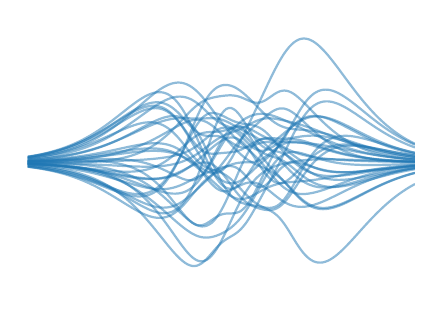
\begin{tikzpicture}
\begin{axis}[axis lines={none}, height={5cm}, width={6.5cm}, xmin={0}, xmax={1}, ymin={-1}, ymax={1}]
    \node at (0,-1) {};
    \node at (0,1) {};
    \node at (1,1) {};
    \node at (1,-1) {};
    \addplot[no markers, smooth, thick, color={rgb,1:red,0.1216;green,0.4667;blue,0.7059}, opacity={0.5}]
        coordinates {
            (0.0,-0.010502713616377508)
            (0.0125,-0.012149540321537382)
            (0.025,-0.014042450032741292)
            (0.0375,-0.01621563612615264)
            (0.05,-0.0187074823410963)
            (0.0625,-0.021560948700236483)
            (0.075,-0.02482396099780444)
            (0.0875,-0.028549793484990506)
            (0.1,-0.032797430876204674)
            (0.1125,-0.037631891476471495)
            (0.125,-0.04312448793816798)
            (0.1375,-0.049352995724360096)
            (0.15,-0.0564016915959917)
            (0.1625,-0.06436121514199522)
            (0.175,-0.07332819530941344)
            (0.1875,-0.08340457082748111)
            (0.2,-0.09469651811423238)
            (0.2125,-0.10731288247413556)
            (0.225,-0.12136298793518142)
            (0.2375,-0.13695367778228953)
            (0.25,-0.1541854116607203)
            (0.2625,-0.17314721613191547)
            (0.275,-0.19391025406356727)
            (0.2875,-0.21651974483626604)
            (0.3,-0.24098493310340563)
            (0.3125,-0.26726677041675734)
            (0.325,-0.2952629439390188)
            (0.3375,-0.32478986336448673)
            (0.35,-0.35556120625807575)
            (0.3625,-0.3871626305558547)
            (0.375,-0.4190223009260154)
            (0.3875,-0.45037695663904087)
            (0.4,-0.4802333908180984)
            (0.4125,-0.5073283163593503)
            (0.425,-0.5301596864765918)
            (0.4375,-0.5472146868107232)
            (0.45,-0.5573087370028212)
            (0.4625,-0.5599931168205065)
            (0.475,-0.5557757526275464)
            (0.4875,-0.5456984281140977)
            (0.5,-0.5307063766671286)
            (0.5125,-0.5110523696733651)
            (0.525,-0.4859761927158391)
            (0.5375,-0.4540980914272316)
            (0.55,-0.4140956063042535)
            (0.5625,-0.36543082832247814)
            (0.575,-0.30887983101211625)
            (0.5875,-0.24641272378239568)
            (0.6,-0.18091404942415404)
            (0.6125,-0.11601445356100741)
            (0.625,-0.055858331539022484)
            (0.6375,-0.0045149625871364)
            (0.65,0.034793961071660225)
            (0.6625,0.060569754957374725)
            (0.675,0.07357257010309093)
            (0.6875,0.07621132741749892)
            (0.7,0.07159173860588028)
            (0.7125,0.06266611362861685)
            (0.725,0.0516511438528635)
            (0.7375,0.040034588256970656)
            (0.75,0.02877043434697735)
            (0.7625,0.0184323999263699)
            (0.775,0.009328117237876854)
            (0.7875,0.001583365343255279)
            (0.8,-0.004796405310656527)
            (0.8125,-0.009881670782322511)
            (0.825,-0.013787262230505852)
            (0.8375,-0.016650340014609955)
            (0.85,-0.018615409282827247)
            (0.8625,-0.01982447759875485)
            (0.875,-0.02041092159566818)
            (0.8875,-0.020495988289743177)
            (0.9,-0.02018713139666294)
            (0.9125,-0.019577592530492908)
            (0.925,-0.0187467962213348)
            (0.9375,-0.01776124777430434)
            (0.95,-0.016675713091493585)
            (0.9625,-0.015534526690336897)
            (0.975,-0.01437292371614606)
            (0.9875,-0.013218327979247626)
            (1.0,-0.012091554205560764)
        }
        ;
    \addplot[no markers, smooth, thick, color={rgb,1:red,0.1216;green,0.4667;blue,0.7059}, opacity={0.5}]
        coordinates {
            (0.0,0.030279177342230092)
            (0.0125,0.03448090583031556)
            (0.025,0.03920149883041725)
            (0.0375,0.044491149291929516)
            (0.05,0.05040169429831759)
            (0.0625,0.05698576676247457)
            (0.075,0.06429565025155291)
            (0.0875,0.07238177541943538)
            (0.1,0.08129078879632612)
            (0.1125,0.0910631173993487)
            (0.125,0.10172994650190112)
            (0.1375,0.1133095239671897)
            (0.15,0.12580270427429133)
            (0.1625,0.13918765077393405)
            (0.175,0.1534136285905982)
            (0.1875,0.16839384671531396)
            (0.2,0.18399735128906572)
            (0.2125,0.20004003963843683)
            (0.225,0.21627496528023035)
            (0.2375,0.23238224970923366)
            (0.25,0.24795912286845917)
            (0.2625,0.2625109010804041)
            (0.275,0.27544410531273056)
            (0.2875,0.2860634582225644)
            (0.3,0.2935752197527257)
            (0.3125,0.29710028521438575)
            (0.325,0.29570175015103134)
            (0.3375,0.2884333369222484)
            (0.35,0.27441729925930564)
            (0.3625,0.2529633267504995)
            (0.375,0.22374375723571846)
            (0.3875,0.18704532068476173)
            (0.4,0.1441239999038181)
            (0.4125,0.09767732188696845)
            (0.425,0.05196252799328958)
            (0.4375,0.011735066430645385)
            (0.45,-0.019294659792095232)
            (0.4625,-0.04011278041368199)
            (0.475,-0.05334397291114181)
            (0.4875,-0.06400644024812786)
            (0.5,-0.07752209082934672)
            (0.5125,-0.09777223676876609)
            (0.525,-0.1257931145812887)
            (0.5375,-0.16020940304293912)
            (0.55,-0.1982001118659139)
            (0.5625,-0.23632553737969791)
            (0.575,-0.27126017222917703)
            (0.5875,-0.30048648193052935)
            (0.6,-0.32307150432497284)
            (0.6125,-0.34060709141511236)
            (0.625,-0.35758233756694674)
            (0.6375,-0.37988166669943624)
            (0.65,-0.41257668276317233)
            (0.6625,-0.4576430234222591)
            (0.675,-0.5125711701744624)
            (0.6875,-0.5716331910762572)
            (0.7,-0.6280358738790605)
            (0.7125,-0.6759866030771596)
            (0.725,-0.7121138364315008)
            (0.7375,-0.7352041575259061)
            (0.75,-0.7454525977224359)
            (0.7625,-0.743907604489061)
            (0.775,-0.7320829275814581)
            (0.7875,-0.7116924960717786)
            (0.8,-0.6844750171590582)
            (0.8125,-0.6520832384785048)
            (0.825,-0.6160191190738384)
            (0.8375,-0.5776009746270305)
            (0.85,-0.5379523328952577)
            (0.8625,-0.4980050163376341)
            (0.875,-0.4585110644177837)
            (0.8875,-0.42005967697724383)
            (0.9,-0.38309652603502925)
            (0.9125,-0.347943642330686)
            (0.925,-0.3148187091325408)
            (0.9375,-0.28385304654742183)
            (0.95,-0.25510788881321367)
            (0.9625,-0.2285887785397839)
            (0.975,-0.20425805128850436)
            (0.9875,-0.1820454807463414)
            (1.0,-0.16185721377255816)
        }
        ;
    \addplot[no markers, smooth, thick, color={rgb,1:red,0.1216;green,0.4667;blue,0.7059}, opacity={0.5}]
        coordinates {
            (0.0,-0.0108469416913144)
            (0.0125,-0.012378378197373823)
            (0.025,-0.014104521058387064)
            (0.0375,-0.016045475129137055)
            (0.05,-0.018222353319017587)
            (0.0625,-0.02065703876584742)
            (0.075,-0.023371846763738532)
            (0.0875,-0.02638906344211578)
            (0.1,-0.029730334631696265)
            (0.1125,-0.0334158746373663)
            (0.125,-0.03746346092302898)
            (0.1375,-0.041887177239667325)
            (0.15,-0.0466958648505471)
            (0.1625,-0.05189123973832224)
            (0.175,-0.05746563373890109)
            (0.1875,-0.06339932043632959)
            (0.2,-0.06965739374070266)
            (0.2125,-0.07618618021201742)
            (0.225,-0.08290918787784309)
            (0.2375,-0.08972262784226659)
            (0.25,-0.09649059479635734)
            (0.2625,-0.10304006441081505)
            (0.275,-0.10915596711590694)
            (0.2875,-0.11457673886834674)
            (0.3,-0.11899094306404873)
            (0.3125,-0.1220358204898016)
            (0.325,-0.12329897770334636)
            (0.3375,-0.1223248962992125)
            (0.35,-0.11862857188891464)
            (0.3625,-0.11171941810075746)
            (0.375,-0.10113965606951732)
            (0.3875,-0.08652282851650478)
            (0.4,-0.06767992488663654)
            (0.4125,-0.04471981446418762)
            (0.425,-0.018136541381833182)
            (0.4375,0.011257158044034647)
            (0.45,0.04243126040148417)
            (0.4625,0.07420792415344794)
            (0.475,0.10527205319853705)
            (0.4875,0.1340718300959203)
            (0.5,0.1586627835485027)
            (0.5125,0.1765313119588495)
            (0.525,0.18462085444869727)
            (0.5375,0.1799458620333158)
            (0.55,0.1604973474508342)
            (0.5625,0.12628916418090505)
            (0.575,0.08003015060250092)
            (0.5875,0.026493013107369946)
            (0.6,-0.028498810197050244)
            (0.6125,-0.07896470003333783)
            (0.625,-0.11951447607035626)
            (0.6375,-0.14586223878499388)
            (0.65,-0.15537188266214325)
            (0.6625,-0.1478018601231424)
            (0.675,-0.12571148484170866)
            (0.6875,-0.09355977983579228)
            (0.7,-0.05640581903504875)
            (0.7125,-0.018704825037669296)
            (0.725,0.016511678353476337)
            (0.7375,0.04751902280144109)
            (0.75,0.07350233588283069)
            (0.7625,0.09425427431781912)
            (0.775,0.10995650824605717)
            (0.7875,0.12102398004602904)
            (0.8,0.12799588306176232)
            (0.8125,0.13146112450404468)
            (0.825,0.1320089915774712)
            (0.8375,0.13019801902879882)
            (0.85,0.12653780832693304)
            (0.8625,0.12147989040348389)
            (0.875,0.11541474705548593)
            (0.8875,0.10867288266386999)
            (0.9,0.1015284240796263)
            (0.9125,0.09420416630213173)
            (0.925,0.08687730913256052)
            (0.9375,0.07968537190935783)
            (0.95,0.07273195031434533)
            (0.9625,0.06609210698249561)
            (0.975,0.059817278500136115)
            (0.9875,0.05393964472586383)
            (1.0,0.0484759493885393)
        }
        ;
    \addplot[no markers, smooth, thick, color={rgb,1:red,0.1216;green,0.4667;blue,0.7059}, opacity={0.5}]
        coordinates {
            (0.0,-0.0018479153865540148)
            (0.0125,-0.0019665920491254455)
            (0.025,-0.0020687484575244905)
            (0.0375,-0.0021451761977938303)
            (0.05,-0.0021841075933709685)
            (0.0625,-0.0021706601206212374)
            (0.075,-0.0020861824131465155)
            (0.0875,-0.0019074893178235464)
            (0.1,-0.0016059733737367426)
            (0.1125,-0.0011465806692574523)
            (0.125,-0.0004866406115994642)
            (0.1375,0.00042545785336900265)
            (0.15,0.0016517460324478152)
            (0.1625,0.003266305991373633)
            (0.175,0.005357034965046341)
            (0.1875,0.00802751027752315)
            (0.2,0.011398898015298666)
            (0.2125,0.015611816333136184)
            (0.225,0.02082802002736808)
            (0.2375,0.027231713172831868)
            (0.25,0.03503021640677145)
            (0.2625,0.044453608721951865)
            (0.275,0.05575282254875231)
            (0.2875,0.06919548543007391)
            (0.3,0.08505855893496023)
            (0.3125,0.10361650934509965)
            (0.325,0.12512333441520898)
            (0.3375,0.1497862399466507)
            (0.35,0.17772807584161923)
            (0.3625,0.20893476177224912)
            (0.375,0.24318280463648423)
            (0.3875,0.27994056678950247)
            (0.4,0.3182351015081254)
            (0.4125,0.356482071902901)
            (0.425,0.3924683434532757)
            (0.4375,0.42381747617279886)
            (0.45,0.4486717479866896)
            (0.4625,0.46644946985029256)
            (0.475,0.4782443181674749)
            (0.4875,0.4860890609701106)
            (0.5,0.49182603933545777)
            (0.5125,0.4959977785189302)
            (0.525,0.49730546663152325)
            (0.5375,0.49361971656455206)
            (0.55,0.48361138598451414)
            (0.5625,0.4684862950769115)
            (0.575,0.452860052722209)
            (0.5875,0.4430556565938566)
            (0.6,0.44443250737083995)
            (0.6125,0.45862736842075863)
            (0.625,0.4819363345962414)
            (0.6375,0.5070585234492203)
            (0.65,0.526002080632471)
            (0.6625,0.5329436570673812)
            (0.675,0.5261174906756436)
            (0.6875,0.5070379543682628)
            (0.7,0.4788965401629028)
            (0.7125,0.4451666548558901)
            (0.725,0.4086396137841888)
            (0.7375,0.37131353870681844)
            (0.75,0.33457573592281387)
            (0.7625,0.29935471771366107)
            (0.775,0.26623783372927046)
            (0.7875,0.23556187193188458)
            (0.8,0.20748247004421413)
            (0.8125,0.18202696518050798)
            (0.825,0.15913434122909492)
            (0.8375,0.13868516206505443)
            (0.85,0.12052376472597537)
            (0.8625,0.10447449884202485)
            (0.875,0.09035341160217494)
            (0.8875,0.07797647105886997)
            (0.9,0.06716517833158807)
            (0.9125,0.057750228201638824)
            (0.925,0.049573727230375265)
            (0.9375,0.042490360507328837)
            (0.95,0.036367805748391706)
            (0.9625,0.031086621372985235)
            (0.975,0.02653977913086658)
            (0.9875,0.02263196842957196)
            (1.0,0.019278766033904195)
        }
        ;
    \addplot[no markers, smooth, thick, color={rgb,1:red,0.1216;green,0.4667;blue,0.7059}, opacity={0.5}]
        coordinates {
            (0.0,0.016521211647219928)
            (0.0125,0.018976710652381455)
            (0.025,0.021771278103347697)
            (0.0375,0.02494618291574114)
            (0.05,0.028546478013181407)
            (0.0625,0.03262104506754899)
            (0.075,0.0372225451073106)
            (0.0875,0.0424072440382509)
            (0.1,0.048234675331521336)
            (0.1125,0.05476709425977974)
            (0.125,0.06206866902532905)
            (0.1375,0.07020434387682026)
            (0.15,0.07923829785482132)
            (0.1625,0.08923191021859686)
            (0.175,0.10024113007559171)
            (0.1875,0.11231313361010618)
            (0.2,0.12548213816212664)
            (0.2125,0.13976422912579814)
            (0.225,0.15515104452887687)
            (0.2375,0.17160215510335483)
            (0.25,0.18903597731657404)
            (0.2625,0.20731906687920487)
            (0.275,0.2262536657140726)
            (0.2875,0.24556342307202206)
            (0.3,0.264877290565267)
            (0.3125,0.2837117135430814)
            (0.325,0.3014514235970853)
            (0.3375,0.3173294003039492)
            (0.35,0.33040694243856916)
            (0.3625,0.33955530615680257)
            (0.375,0.34344107728454276)
            (0.3875,0.3405184080453865)
            (0.4,0.3290325443245775)
            (0.4125,0.3070457275746084)
            (0.425,0.27261829666544996)
            (0.4375,0.22436928328975256)
            (0.45,0.16228238340401638)
            (0.4625,0.08869102063296734)
            (0.475,0.008779615271503727)
            (0.4875,-0.07057579774230886)
            (0.5,-0.14255257563135534)
            (0.5125,-0.2021341595023495)
            (0.525,-0.24730408275749383)
            (0.5375,-0.2786275739169653)
            (0.55,-0.2983866436728292)
            (0.5625,-0.30992058053143173)
            (0.575,-0.3169996101710131)
            (0.5875,-0.32295255464722966)
            (0.6,-0.3296465482524926)
            (0.6125,-0.3363602626888577)
            (0.625,-0.3392795415885615)
            (0.6375,-0.33292702790474554)
            (0.65,-0.31232792703903417)
            (0.6625,-0.27526441630425635)
            (0.675,-0.22369076416067007)
            (0.6875,-0.16262225021297108)
            (0.7,-0.09821508133430955)
            (0.7125,-0.035987104229345174)
            (0.725,0.020400886117503174)
            (0.7375,0.06901435532003562)
            (0.75,0.10910603209516007)
            (0.7625,0.14070681160553072)
            (0.775,0.1643318681923863)
            (0.7875,0.18077285612155497)
            (0.8,0.19095395014721803)
            (0.8125,0.19583480434960363)
            (0.825,0.19634762372429984)
            (0.8375,0.19335871329957321)
            (0.85,0.1876473027291078)
            (0.8625,0.17989630433688494)
            (0.875,0.1706910781614046)
            (0.8875,0.16052334945346722)
            (0.9,0.14979823110812715)
            (0.9125,0.13884290710378897)
            (0.925,0.12791598098618717)
            (0.9375,0.11721682287052762)
            (0.95,0.10689448804707888)
            (0.9625,0.09705595220500336)
            (0.975,0.08777352955493434)
            (0.9875,0.07909142376235799)
            (1.0,0.07103141753385081)
        }
        ;
    \addplot[no markers, smooth, thick, color={rgb,1:red,0.1216;green,0.4667;blue,0.7059}, opacity={0.5}]
        coordinates {
            (0.0,-0.03246001667087368)
            (0.0125,-0.03688994940568411)
            (0.025,-0.041849640105160166)
            (0.0375,-0.04738599400125608)
            (0.05,-0.05354613019989036)
            (0.0625,-0.060376161923444964)
            (0.075,-0.06791960339622534)
            (0.0875,-0.07621532931291822)
            (0.1,-0.08529500383174242)
            (0.1125,-0.09517988761937163)
            (0.125,-0.10587692449864841)
            (0.1375,-0.11737400494192361)
            (0.15,-0.1296343037438975)
            (0.1625,-0.14258959609758068)
            (0.175,-0.15613247326866506)
            (0.1875,-0.17010741056299905)
            (0.2,-0.18430069227686488)
            (0.2125,-0.1984292787628348)
            (0.225,-0.21212882016525827)
            (0.2375,-0.2249411936458635)
            (0.25,-0.23630218420489132)
            (0.2625,-0.24553026722233043)
            (0.275,-0.25181791442714085)
            (0.2875,-0.25422747409199253)
            (0.3,-0.25169452243333745)
            (0.3125,-0.24304271290950585)
            (0.325,-0.2270156486985225)
            (0.3375,-0.20233328047594137)
            (0.35,-0.16778292656459748)
            (0.3625,-0.12235840408186516)
            (0.375,-0.06546517522636165)
            (0.3875,0.002784858572124488)
            (0.4,0.08115787324573642)
            (0.4125,0.16674131113790086)
            (0.425,0.25469654901231126)
            (0.4375,0.3391142521119993)
            (0.45,0.41427784758842345)
            (0.4625,0.4759662185153116)
            (0.475,0.522320368518212)
            (0.4875,0.5533947777259418)
            (0.5,0.5703442968981071)
            (0.5125,0.5747827547665842)
            (0.525,0.568358755265208)
            (0.5375,0.5526450559859076)
            (0.55,0.5291782990712073)
            (0.5625,0.4995537971294121)
            (0.575,0.4655104967816775)
            (0.5875,0.4289040119296553)
            (0.6,0.3916615219525218)
            (0.6125,0.3557677935000849)
            (0.625,0.3232057243786354)
            (0.6375,0.29572538314918567)
            (0.65,0.2745197092289941)
            (0.6625,0.25984494281105563)
            (0.675,0.25080786594972465)
            (0.6875,0.2457203291945259)
            (0.7,0.24263620176419318)
            (0.7125,0.23986087976278847)
            (0.725,0.2363010308673879)
            (0.7375,0.23140518860496295)
            (0.75,0.2249848091154103)
            (0.7625,0.21708084356004773)
            (0.775,0.2078696031751662)
            (0.7875,0.19759766275145027)
            (0.8,0.186538026846953)
            (0.8125,0.17496169351244492)
            (0.825,0.16312021792310516)
            (0.8375,0.15123600149077807)
            (0.85,0.13949788801195734)
            (0.8625,0.12806029768630714)
            (0.875,0.11704461970999369)
            (0.8875,0.10654195149656459)
            (0.9,0.09661654611121763)
            (0.9125,0.08730953150446531)
            (0.925,0.07864261284512744)
            (0.9375,0.0706215759896585)
            (0.95,0.06323948612051647)
            (0.9625,0.05647952868306262)
            (0.975,0.05031747593206157)
            (0.9875,0.04472378620906541)
            (1.0,0.03966535794314407)
        }
        ;
    \addplot[no markers, smooth, thick, color={rgb,1:red,0.1216;green,0.4667;blue,0.7059}, opacity={0.5}]
        coordinates {
            (0.0,0.03564118381896324)
            (0.0125,0.040651910671922135)
            (0.025,0.04629562179234412)
            (0.0375,0.05263688974390959)
            (0.05,0.05974335585823704)
            (0.0625,0.0676849281618556)
            (0.075,0.07653265510292846)
            (0.0875,0.08635720318598038)
            (0.1,0.09722685635917436)
            (0.1125,0.10920494469068755)
            (0.125,0.12234660016526294)
            (0.1375,0.13669472929072402)
            (0.15,0.15227508701530967)
            (0.1625,0.16909033618097627)
            (0.175,0.18711298409963856)
            (0.1875,0.20627710657398193)
            (0.2,0.22646880485893128)
            (0.2125,0.24751539948649637)
            (0.225,0.2691734556458342)
            (0.2375,0.2911158699737827)
            (0.25,0.31291844405765223)
            (0.2625,0.3340466465264776)
            (0.275,0.3538436505365638)
            (0.2875,0.37152126216904025)
            (0.3,0.38615607368615606)
            (0.3125,0.3966941431112348)
            (0.325,0.40196879472526825)
            (0.3375,0.4007378521741915)
            (0.35,0.3917488830939863)
            (0.3625,0.37384401288322616)
            (0.375,0.34611976157724605)
            (0.3875,0.3081624343650969)
            (0.4,0.2603861873102282)
            (0.4125,0.2044935845429706)
            (0.425,0.14370564670312988)
            (0.4375,0.0821383642142071)
            (0.45,0.02388531086462285)
            (0.4625,-0.02789184905400661)
            (0.475,-0.0715301480568661)
            (0.4875,-0.10646998664126317)
            (0.5,-0.1325572086159001)
            (0.5125,-0.14941677740972042)
            (0.525,-0.15614709167237362)
            (0.5375,-0.15177941146965274)
            (0.55,-0.13608044271299943)
            (0.5625,-0.11046320352379503)
            (0.575,-0.07840500324654423)
            (0.5875,-0.044310494128123115)
            (0.6,-0.011787190947896702)
            (0.6125,0.018136996899180604)
            (0.625,0.04797629790410746)
            (0.6375,0.08234765543298031)
            (0.65,0.12565877922125007)
            (0.6625,0.17976320232091803)
            (0.675,0.24249962518512552)
            (0.6875,0.30877986816947306)
            (0.7,0.37252740862844397)
            (0.7125,0.4285286980838769)
            (0.725,0.473704978998312)
            (0.7375,0.5068910215309967)
            (0.75,0.5281793326635721)
            (0.7625,0.5384329062448581)
            (0.775,0.5389431516926868)
            (0.7875,0.5311950251756677)
            (0.8,0.5167105618809561)
            (0.8125,0.4969490828787329)
            (0.825,0.47324778718353855)
            (0.8375,0.4467906022813244)
            (0.85,0.4185963399406595)
            (0.8625,0.3895196121367979)
            (0.875,0.3602597792440758)
            (0.8875,0.331374565759092)
            (0.9,0.3032959939496259)
            (0.9125,0.27634703549744016)
            (0.925,0.25075792931986157)
            (0.9375,0.22668150965683678)
            (0.95,0.20420717016548387)
            (0.9625,0.18337328628183056)
            (0.975,0.16417805171295485)
            (0.9875,0.14658877249895164)
            (1.0,0.13054971639712204)
        }
        ;
    \addplot[no markers, smooth, thick, color={rgb,1:red,0.1216;green,0.4667;blue,0.7059}, opacity={0.5}]
        coordinates {
            (0.0,0.04124430542024027)
            (0.0125,0.04710028979120266)
            (0.025,0.05370854762116014)
            (0.0375,0.06114871593504615)
            (0.05,0.06950500693585235)
            (0.0625,0.07886546063963548)
            (0.075,0.08932084678176169)
            (0.0875,0.10096313386093224)
            (0.1,0.11388343043958829)
            (0.1125,0.12816929056162268)
            (0.125,0.1439012619664051)
            (0.1375,0.16114854357182556)
            (0.15,0.17996360879772927)
            (0.1625,0.20037564561487903)
            (0.175,0.2223826654223574)
            (0.1875,0.24594214470366)
            (0.2,0.2709600909856686)
            (0.2125,0.2972784748269449)
            (0.225,0.32466105165740017)
            (0.2375,0.35277772362762033)
            (0.25,0.38118777855449265)
            (0.2625,0.4093226121069402)
            (0.275,0.4364689187913005)
            (0.2875,0.46175386391610995)
            (0.3,0.48413447045012115)
            (0.3125,0.5023944336166379)
            (0.325,0.5151528923893797)
            (0.3375,0.5208914440780398)
            (0.35,0.5180080186523033)
            (0.3625,0.5049093034954699)
            (0.375,0.4801574445232683)
            (0.3875,0.4426920238299746)
            (0.4,0.3921551811420693)
            (0.4125,0.32934432957635174)
            (0.425,0.2565296532517538)
            (0.4375,0.17716720872896644)
            (0.45,0.09546405903029982)
            (0.4625,0.016043462833255806)
            (0.475,-0.05634945769290148)
            (0.4875,-0.117181913842362)
            (0.5,-0.1625337150031513)
            (0.5125,-0.18959705153849812)
            (0.525,-0.19710179396601904)
            (0.5375,-0.18533391925648812)
            (0.55,-0.15614370168266312)
            (0.5625,-0.11316709008009851)
            (0.575,-0.06180758502075846)
            (0.5875,-0.008194648385388234)
            (0.6,0.04224402558864042)
            (0.6125,0.08625958236057378)
            (0.625,0.123656674978658)
            (0.6375,0.15637244396990935)
            (0.65,0.18696476885985883)
            (0.6625,0.2171776369593551)
            (0.675,0.24701616485524128)
            (0.6875,0.2751254817687138)
            (0.7,0.2996184205086656)
            (0.7125,0.3188751172432314)
            (0.725,0.3320970915925061)
            (0.7375,0.3392202559302903)
            (0.75,0.34064184617597093)
            (0.7625,0.33702034555595023)
            (0.775,0.32913776641511994)
            (0.7875,0.31780756742041877)
            (0.8,0.30381558861622027)
            (0.8125,0.28788454178317363)
            (0.825,0.2706550092278975)
            (0.8375,0.2526777459947147)
            (0.85,0.2344134782373838)
            (0.8625,0.21623744555092828)
            (0.875,0.19844672659756013)
            (0.8875,0.18126897699806702)
            (0.9,0.16487164406333918)
            (0.9125,0.14937104157917006)
            (0.925,0.1348408981522003)
            (0.9375,0.12132015660118663)
            (0.95,0.10881991642196477)
            (0.9625,0.09732948935904229)
            (0.975,0.08682158937932562)
            (0.9875,0.07725671026996364)
            (1.0,0.06858676223694168)
        }
        ;
    \addplot[no markers, smooth, thick, color={rgb,1:red,0.1216;green,0.4667;blue,0.7059}, opacity={0.5}]
        coordinates {
            (0.0,-0.02446088904119238)
            (0.0125,-0.02801459051448421)
            (0.025,-0.032041787679332474)
            (0.0375,-0.03659635863069062)
            (0.05,-0.041736231508537794)
            (0.0625,-0.04752316087859833)
            (0.075,-0.054022319951770155)
            (0.0875,-0.06130165842811016)
            (0.1,-0.06943096615308174)
            (0.1125,-0.07848057201530131)
            (0.125,-0.08851959565975555)
            (0.1375,-0.09961365680457364)
            (0.15,-0.11182193354675143)
            (0.1625,-0.1251934475447058)
            (0.175,-0.13976244118364378)
            (0.1875,-0.15554270096864312)
            (0.2,-0.1725206741898382)
            (0.2125,-0.19064722482138843)
            (0.225,-0.20982788306392142)
            (0.2375,-0.22991146559743542)
            (0.25,-0.2506769868224539)
            (0.2625,-0.27181885365849323)
            (0.275,-0.2929304492154543)
            (0.2875,-0.31348637893000875)
            (0.3,-0.33282389643380894)
            (0.3125,-0.3501243715493494)
            (0.325,-0.36439614341599813)
            (0.3375,-0.37446076208837215)
            (0.35,-0.3789455193845513)
            (0.3625,-0.37628637841351226)
            (0.375,-0.36474702657728003)
            (0.3875,-0.34246192164829603)
            (0.4,-0.3075140320930511)
            (0.4125,-0.2580663286639791)
            (0.425,-0.19268332549369016)
            (0.4375,-0.11106851206909851)
            (0.45,-0.015110805203465116)
            (0.4625,0.08981307767383795)
            (0.475,0.19427037826575871)
            (0.4875,0.2866859880327929)
            (0.5,0.3561931867385024)
            (0.5125,0.39560044066137867)
            (0.525,0.4034220725275282)
            (0.5375,0.3830289001571921)
            (0.55,0.3410223221060192)
            (0.5625,0.2860041175471363)
            (0.575,0.22745940957121186)
            (0.5875,0.17430877745238618)
            (0.6,0.13323568359297389)
            (0.6125,0.10681325606807693)
            (0.625,0.09248161555628359)
            (0.6375,0.0842901395961697)
            (0.65,0.07556254744819642)
            (0.6625,0.061476249781997686)
            (0.675,0.04074661543964408)
            (0.6875,0.01492008762400989)
            (0.7,-0.0131044231862627)
            (0.7125,-0.040419048004747694)
            (0.725,-0.06503802363288881)
            (0.7375,-0.08590340766347707)
            (0.75,-0.10259635214617284)
            (0.7625,-0.11511612801989164)
            (0.775,-0.12372163606973477)
            (0.7875,-0.12881955485510307)
            (0.8,-0.13088702742215333)
            (0.8125,-0.13041969393964045)
            (0.825,-0.12789812078900592)
            (0.8375,-0.12376740323072509)
            (0.85,-0.11842604279058394)
            (0.8625,-0.11222121172059157)
            (0.875,-0.10544828568949088)
            (0.8875,-0.09835310736133535)
            (0.9,-0.09113588078014864)
            (0.9125,-0.08395592305266777)
            (0.925,-0.0769367418021357)
            (0.9375,-0.07017108448688365)
            (0.95,-0.06372573458287542)
            (0.9625,-0.057645921875596876)
            (0.975,-0.05195927895281966)
            (0.9875,-0.046679320517632496)
            (1.0,-0.041808451742993614)
        }
        ;
    \addplot[no markers, smooth, thick, color={rgb,1:red,0.1216;green,0.4667;blue,0.7059}, opacity={0.5}]
        coordinates {
            (0.0,-0.03132482496251164)
            (0.0125,-0.035577286026011276)
            (0.025,-0.0403335104737785)
            (0.0375,-0.04563701226499533)
            (0.05,-0.05153118202267943)
            (0.0625,-0.05805806351986668)
            (0.075,-0.06525676780019092)
            (0.0875,-0.07316145520193046)
            (0.1,-0.08179880780066395)
            (0.1125,-0.09118490792974214)
            (0.125,-0.10132143340834478)
            (0.1375,-0.1121910782233709)
            (0.15,-0.12375211051519848)
            (0.1625,-0.13593199034210773)
            (0.175,-0.14861999129061984)
            (0.1875,-0.16165880720389403)
            (0.2,-0.174835184327285)
            (0.2125,-0.1878697082652131)
            (0.225,-0.20040600519275026)
            (0.2375,-0.21199980206697316)
            (0.25,-0.22210854983243908)
            (0.2625,-0.23008267115880762)
            (0.275,-0.2351599816784893)
            (0.2875,-0.23646549186992863)
            (0.3,-0.23301967835191661)
            (0.3125,-0.22375948618837377)
            (0.325,-0.20757787480159512)
            (0.3375,-0.18338976055672163)
            (0.35,-0.150234881189356)
            (0.3625,-0.10743159226629845)
            (0.375,-0.05480013448198778)
            (0.3875,0.0070202241186370015)
            (0.4,0.0761281931579829)
            (0.4125,0.14877338944132007)
            (0.425,0.219164246930172)
            (0.4375,0.28061580601485087)
            (0.45,0.3272330219686137)
            (0.4625,0.3557047593909504)
            (0.475,0.3664634858581522)
            (0.4875,0.3628483504891635)
            (0.5,0.34968132427207904)
            (0.5125,0.33203644300200125)
            (0.525,0.31428270349736015)
            (0.5375,0.29958610748934145)
            (0.55,0.2894976972222525)
            (0.5625,0.28340515827893975)
            (0.575,0.2783444740474442)
            (0.5875,0.2700648042064818)
            (0.6,0.2545573118703531)
            (0.6125,0.22962473791263618)
            (0.625,0.1958787237784355)
            (0.6375,0.15604267420427118)
            (0.65,0.11371778896156755)
            (0.6625,0.07225448034063207)
            (0.675,0.03397488893496017)
            (0.6875,0.00020958866797880955)
            (0.7,-0.028416172136124605)
            (0.7125,-0.05177059331185112)
            (0.725,-0.07006139857879884)
            (0.7375,-0.08370650833442164)
            (0.75,-0.09323499354976958)
            (0.7625,-0.09921903031600825)
            (0.775,-0.10222886800092112)
            (0.7875,-0.1028044274597675)
            (0.8,-0.10143874039807692)
            (0.8125,-0.09856966275006183)
            (0.825,-0.09457722709445049)
            (0.8375,-0.08978470698074735)
            (0.85,-0.08446200068718673)
            (0.8625,-0.07883034328557166)
            (0.875,-0.07306765504210329)
            (0.8875,-0.0673140553032511)
            (0.9,-0.061677232831660135)
            (0.9125,-0.05623748054314994)
            (0.925,-0.05105228589863397)
            (0.9375,-0.04616042637902383)
            (0.95,-0.04158555905315679)
            (0.9625,-0.03733931921148275)
            (0.975,-0.03342395914417542)
            (0.9875,-0.029834567221341663)
            (1.0,-0.026560911599164846)
        }
        ;
    \addplot[no markers, smooth, thick, color={rgb,1:red,0.1216;green,0.4667;blue,0.7059}, opacity={0.5}]
        coordinates {
            (0.0,-0.01586207692306112)
            (0.0125,-0.018106829868483092)
            (0.025,-0.0206385470234529)
            (0.0375,-0.023487341131883218)
            (0.05,-0.02668500065284553)
            (0.0625,-0.030264695390346864)
            (0.075,-0.03426054910072831)
            (0.0875,-0.03870704878867959)
            (0.1,-0.04363825600385588)
            (0.1125,-0.04908678101713799)
            (0.125,-0.05508247656121764)
            (0.1375,-0.061650804270895615)
            (0.15,-0.06881082464238415)
            (0.1625,-0.07657276108025154)
            (0.175,-0.0849350915734621)
            (0.1875,-0.0938811293279043)
            (0.2,-0.10337506844052577)
            (0.2125,-0.1133574953345469)
            (0.225,-0.12374040506551742)
            (0.2375,-0.13440181890086708)
            (0.25,-0.14518018256076823)
            (0.2625,-0.1558688420981205)
            (0.275,-0.16621105823794824)
            (0.2875,-0.17589624525429823)
            (0.3,-0.18455842680493892)
            (0.3125,-0.19177831400400977)
            (0.325,-0.19709096318254826)
            (0.3375,-0.2000017044341563)
            (0.35,-0.20001400126200689)
            (0.3625,-0.1966741756699587)
            (0.375,-0.18963960031211008)
            (0.3875,-0.1787791325739008)
            (0.4,-0.16431738818275757)
            (0.4125,-0.14703026923094964)
            (0.425,-0.1283139161179295)
            (0.4375,-0.10981467325610142)
            (0.45,-0.09289178279579009)
            (0.4625,-0.0780630739116973)
            (0.475,-0.06478495845963853)
            (0.4875,-0.0521946107621659)
            (0.5,-0.04023975753997943)
            (0.5125,-0.030872238769281427)
            (0.525,-0.028475049150597714)
            (0.5375,-0.03805354945112145)
            (0.55,-0.0624918637327007)
            (0.5625,-0.09958692922177935)
            (0.575,-0.14056209196067293)
            (0.5875,-0.17309937544799664)
            (0.6,-0.18605533037791613)
            (0.6125,-0.17431484849032453)
            (0.625,-0.14173139723670306)
            (0.6375,-0.09843254932052839)
            (0.65,-0.056242248680440844)
            (0.6625,-0.024292572468004744)
            (0.675,-0.006122034796483088)
            (0.6875,-0.0006510051782827666)
            (0.7,-0.0043932086695982015)
            (0.7125,-0.013417722819483953)
            (0.725,-0.024714077683447758)
            (0.7375,-0.03631949704987698)
            (0.75,-0.0470309363494024)
            (0.7625,-0.0561766269546983)
            (0.775,-0.06344790790376056)
            (0.7875,-0.06877667290124045)
            (0.8,-0.0722471387478576)
            (0.8125,-0.07403327259283483)
            (0.825,-0.07435525978040758)
            (0.8375,-0.07344997823060666)
            (0.85,-0.07155166927359151)
            (0.8625,-0.06887993751264727)
            (0.875,-0.06563293571004404)
            (0.8875,-0.0619841436754567)
            (0.9,-0.05808157097631044)
            (0.9125,-0.054048531967385405)
            (0.925,-0.04998538158643367)
            (0.9375,-0.04597177985381606)
            (0.95,-0.04206918626175895)
            (0.9625,-0.038323383269150156)
            (0.975,-0.03476689946202093)
            (0.9875,-0.0314212541770356)
            (1.0,-0.028298981570564753)
        }
        ;
    \addplot[no markers, smooth, thick, color={rgb,1:red,0.1216;green,0.4667;blue,0.7059}, opacity={0.5}]
        coordinates {
            (0.0,-0.012777284642635443)
            (0.0125,-0.014547991636925271)
            (0.025,-0.016536872688125908)
            (0.0375,-0.018764926122763818)
            (0.05,-0.02125380978963472)
            (0.0625,-0.02402547828141039)
            (0.075,-0.027101694675124355)
            (0.0875,-0.030503391013941533)
            (0.1,-0.03424984858875504)
            (0.1125,-0.03835766613630836)
            (0.125,-0.04283948166383547)
            (0.1375,-0.047702412189055646)
            (0.15,-0.052946175883281495)
            (0.1625,-0.05856086380412615)
            (0.175,-0.06452433480700107)
            (0.1875,-0.07079921896248524)
            (0.2,-0.0773295340702595)
            (0.2125,-0.08403694956976314)
            (0.225,-0.09081677617117404)
            (0.2375,-0.09753382296360431)
            (0.25,-0.10401835328138608)
            (0.2625,-0.11006249494548974)
            (0.275,-0.11541763098741133)
            (0.2875,-0.11979352830638496)
            (0.3,-0.12286027289841649)
            (0.3125,-0.12425449579369202)
            (0.325,-0.12359192508656348)
            (0.3375,-0.12048902674277745)
            (0.35,-0.11459745177553926)
            (0.3625,-0.10565625570644725)
            (0.375,-0.0935684818227466)
            (0.3875,-0.07851080926472596)
            (0.4,-0.061087695862352985)
            (0.4125,-0.04253858515375854)
            (0.425,-0.024856621803586252)
            (0.4375,-0.010568622262936525)
            (0.45,-0.0024026909401133178)
            (0.4625,-0.002959607220332589)
            (0.475,-0.014360069970924906)
            (0.4875,-0.037838097698408936)
            (0.5,-0.0732134600393754)
            (0.5125,-0.11819939059484662)
            (0.525,-0.16812636081255425)
            (0.5375,-0.21710921371834868)
            (0.55,-0.2597521300279887)
            (0.5625,-0.2929028241841869)
            (0.575,-0.3166708358329694)
            (0.5875,-0.33328197294820366)
            (0.6,-0.34519782488109796)
            (0.6125,-0.35329550317415653)
            (0.625,-0.3558159023941346)
            (0.6375,-0.3493617248135662)
            (0.65,-0.33066246734896976)
            (0.6625,-0.29839925145125407)
            (0.675,-0.25436180452667634)
            (0.6875,-0.20262522910233113)
            (0.7,-0.14808992502835924)
            (0.7125,-0.09512862228451621)
            (0.725,-0.04666139438595972)
            (0.7375,-0.0042606588770670575)
            (0.75,0.0314325738743153)
            (0.7625,0.06039208474759224)
            (0.775,0.08297827741364075)
            (0.7875,0.09977622355761734)
            (0.8,0.11148291438980237)
            (0.8125,0.11883076511438591)
            (0.825,0.12253755474415207)
            (0.8375,0.12327540145088296)
            (0.85,0.12165323143677055)
            (0.8625,0.11820862131687959)
            (0.875,0.11340597775336347)
            (0.8875,0.10763884002996287)
            (0.9,0.10123471119961029)
            (0.9125,0.09446128805556729)
            (0.925,0.08753330581373546)
            (0.9375,0.08061946828159487)
            (0.95,0.07384912029375328)
            (0.9625,0.06731845319938687)
            (0.975,0.06109612918620303)
            (0.9875,0.055228276179990834)
            (1.0,0.04974284957278422)
        }
        ;
    \addplot[no markers, smooth, thick, color={rgb,1:red,0.1216;green,0.4667;blue,0.7059}, opacity={0.5}]
        coordinates {
            (0.0,0.009803848392903844)
            (0.0125,0.011180253932989753)
            (0.025,0.012729911886781287)
            (0.0375,0.014470292957667361)
            (0.05,0.01641962527361875)
            (0.0625,0.018596649732335584)
            (0.075,0.0210202798129364)
            (0.0875,0.02370914445271288)
            (0.1,0.026680989358416993)
            (0.1125,0.02995190878099933)
            (0.125,0.0335353764846799)
            (0.1375,0.03744104162062436)
            (0.15,0.041673252817532994)
            (0.1625,0.04622927252020796)
            (0.175,0.05109714413600794)
            (0.1875,0.05625317784630201)
            (0.2,0.06165902831384941)
            (0.2125,0.06725835073576056)
            (0.225,0.07297304312545339)
            (0.2375,0.07869911551001733)
            (0.25,0.08430227507370155)
            (0.2625,0.08961338565282677)
            (0.275,0.09442405757986184)
            (0.2875,0.09848275905758366)
            (0.3,0.10149202519497831)
            (0.3125,0.10310759132148868)
            (0.325,0.10294061356830159)
            (0.3375,0.10056458816477308)
            (0.35,0.0955291750875492)
            (0.3625,0.08738391471735614)
            (0.375,0.07571585309733335)
            (0.3875,0.06020643253303475)
            (0.4,0.04071474913333254)
            (0.4125,0.017392868986600814)
            (0.425,-0.009247191638106961)
            (0.4375,-0.0384573530256742)
            (0.45,-0.06943586340810137)
            (0.4625,-0.10149441428145113)
            (0.475,-0.13411777649006526)
            (0.4875,-0.1667492115923257)
            (0.5,-0.19845925654815108)
            (0.5125,-0.22758850066725395)
            (0.525,-0.2516297002598768)
            (0.5375,-0.26781543296732097)
            (0.55,-0.2740118926920567)
            (0.5625,-0.2697063332388143)
            (0.575,-0.25659930983145884)
            (0.5875,-0.23792065630891435)
            (0.6,-0.21733643068639247)
            (0.6125,-0.1979234825910298)
            (0.625,-0.18147502324353368)
            (0.6375,-0.1686323716421503)
            (0.65,-0.15926951491855)
            (0.6625,-0.15280554859968207)
            (0.675,-0.1484411917687279)
            (0.6875,-0.14531050638334295)
            (0.7,-0.14260160237033093)
            (0.7125,-0.13968144889402792)
            (0.725,-0.13618006096624943)
            (0.7375,-0.13194638404372663)
            (0.75,-0.12697115129923955)
            (0.7625,-0.12133052219316585)
            (0.775,-0.11514691480316284)
            (0.7875,-0.1085624529781867)
            (0.8,-0.10172157085269895)
            (0.8125,-0.09476017929610696)
            (0.825,-0.0877994590561064)
            (0.8375,-0.08094284887674738)
            (0.85,-0.07427517914371315)
            (0.8625,-0.06786319032089257)
            (0.875,-0.061756892200525215)
            (0.8875,-0.0559913816152043)
            (0.9,-0.05058885581562346)
            (0.9125,-0.045560646318986854)
            (0.925,-0.04090916148910816)
            (0.9375,-0.03662967143070805)
            (0.95,-0.032711900574893094)
            (0.9625,-0.02914141511874458)
            (0.975,-0.025900806933494655)
            (0.9875,-0.022970684694645183)
            (1.0,-0.020330488333310172)
        }
        ;
    \addplot[no markers, smooth, thick, color={rgb,1:red,0.1216;green,0.4667;blue,0.7059}, opacity={0.5}]
        coordinates {
            (0.0,-0.03355746233375992)
            (0.0125,-0.038299927002041004)
            (0.025,-0.04364716579189243)
            (0.0375,-0.04966227459002764)
            (0.05,-0.05641175597608397)
            (0.0625,-0.06396486823425708)
            (0.075,-0.07239268778121259)
            (0.0875,-0.08176682012109707)
            (0.1,-0.09215768504150415)
            (0.1125,-0.10363229229748214)
            (0.125,-0.11625141507630854)
            (0.1375,-0.13006606096184217)
            (0.15,-0.14511313517937643)
            (0.1625,-0.16141019037643972)
            (0.175,-0.17894916355306917)
            (0.1875,-0.19768901738851186)
            (0.2,-0.2175472347251566)
            (0.2125,-0.23839016756099593)
            (0.225,-0.26002232384279395)
            (0.2375,-0.2821747976191744)
            (0.25,-0.30449322518414795)
            (0.2625,-0.32652590072048504)
            (0.275,-0.3477130344718672)
            (0.2875,-0.3673786169579967)
            (0.3,-0.3847270061264153)
            (0.3125,-0.39884723482152834)
            (0.325,-0.4087292134395171)
            (0.3375,-0.41329756699992454)
            (0.35,-0.4114709123847003)
            (0.3625,-0.4022570977209747)
            (0.375,-0.3848984802705849)
            (0.3875,-0.35908595197709214)
            (0.4,-0.32526643872582905)
            (0.4125,-0.28506086063998703)
            (0.425,-0.2414432142060212)
            (0.4375,-0.1980656992471953)
            (0.45,-0.1582733315934808)
            (0.4625,-0.12410154578688888)
            (0.475,-0.09568863601064931)
            (0.4875,-0.07189137559200831)
            (0.5,-0.051307375092972354)
            (0.5125,-0.03325918867595922)
            (0.525,-0.01833028654928109)
            (0.5375,-0.00771514043942932)
            (0.55,-0.0021079823403210634)
            (0.5625,-0.0005340600745873637)
            (0.575,0.00024329440839478865)
            (0.5875,0.004612753622023088)
            (0.6,0.016360244918368065)
            (0.6125,0.03684773112321699)
            (0.625,0.06392990408555002)
            (0.6375,0.09306232736485963)
            (0.65,0.11915429734504286)
            (0.6625,0.13836994594056654)
            (0.675,0.14932076404020592)
            (0.6875,0.1526242065354621)
            (0.7,0.14995310618160138)
            (0.7125,0.14320829954315545)
            (0.725,0.1339447240227005)
            (0.7375,0.12329501809166919)
            (0.75,0.11206568719110761)
            (0.7625,0.10081760685746706)
            (0.775,0.08992818028002529)
            (0.7875,0.07963912920973942)
            (0.8,0.07009306293762138)
            (0.8125,0.06136130646145623)
            (0.825,0.05346494173267587)
            (0.8375,0.046390597554327936)
            (0.85,0.04010219226553396)
            (0.8625,0.034549571154211214)
            (0.875,0.029674773466823807)
            (0.8875,0.02541650063560494)
            (0.9,0.021713228895208103)
            (0.9125,0.01850530860748319)
            (0.925,0.015736313609187473)
            (0.9375,0.01335384216692664)
            (0.95,0.011309923024411384)
            (0.9625,0.009561142665905232)
            (0.975,0.008068580999886143)
            (0.9875,0.006797620368386796)
            (1.0,0.005717675670372798)
        }
        ;
    \addplot[no markers, smooth, thick, color={rgb,1:red,0.1216;green,0.4667;blue,0.7059}, opacity={0.5}]
        coordinates {
            (0.0,-0.006568690166724591)
            (0.0125,-0.0077537561664978005)
            (0.025,-0.009146656792778622)
            (0.0375,-0.010782394258489668)
            (0.05,-0.012701504088803005)
            (0.0625,-0.014950835768468845)
            (0.075,-0.017584417432149967)
            (0.0875,-0.020664405536075948)
            (0.1,-0.024262117156417188)
            (0.1125,-0.028459137847535475)
            (0.125,-0.03334849141207511)
            (0.1375,-0.03903584890912644)
            (0.15,-0.045640742021903234)
            (0.1625,-0.05329772958777536)
            (0.175,-0.06215744447450254)
            (0.1875,-0.07238741956430736)
            (0.2,-0.08417255448261803)
            (0.2125,-0.09771503648489438)
            (0.225,-0.11323346657562451)
            (0.2375,-0.1309608616849602)
            (0.25,-0.15114110080836213)
            (0.2625,-0.174023251452973)
            (0.275,-0.19985304505673818)
            (0.2875,-0.22886055690526388)
            (0.3,-0.26124287579140054)
            (0.3125,-0.29714020667460056)
            (0.325,-0.3366034177397735)
            (0.3375,-0.3795504989104654)
            (0.35,-0.4257087138938049)
            (0.3625,-0.4745383672331112)
            (0.375,-0.5251330281462896)
            (0.3875,-0.5760897001692296)
            (0.4,-0.6253407328564361)
            (0.4125,-0.6699465201946697)
            (0.425,-0.7060723636886861)
            (0.4375,-0.7295376409237158)
            (0.45,-0.7366326999325931)
            (0.4625,-0.7250514751117191)
            (0.475,-0.6945719333143107)
            (0.4875,-0.6468090040139455)
            (0.5,-0.5847696212716836)
            (0.5125,-0.5126183788508678)
            (0.525,-0.43542659344649)
            (0.5375,-0.3585261461416636)
            (0.55,-0.28671374819321127)
            (0.5625,-0.2234249669580902)
            (0.575,-0.17019746403689817)
            (0.5875,-0.12702301268397528)
            (0.6,-0.09294563051162527)
            (0.6125,-0.06654586248171326)
            (0.625,-0.04629427673471754)
            (0.6375,-0.03073048105936696)
            (0.65,-0.018575156853012142)
            (0.6625,-0.008841309237861387)
            (0.675,-0.000899334526083211)
            (0.6875,0.0055955172811365935)
            (0.7,0.010817686347108777)
            (0.7125,0.014874740871675103)
            (0.725,0.017881219444701717)
            (0.7375,0.019968006834450453)
            (0.75,0.021270391761672405)
            (0.7625,0.021919634219145546)
            (0.775,0.02203780867264436)
            (0.7875,0.021734961908024104)
            (0.8,0.02110787193208747)
            (0.8125,0.0202398829242671)
            (0.825,0.019201434141336838)
            (0.8375,0.01805100835233144)
            (0.85,0.016836305982660216)
            (0.8625,0.015595511024219513)
            (0.875,0.014358558851335999)
            (0.8875,0.013148348186999337)
            (0.9,0.011981862534979484)
            (0.9125,0.010871182696260567)
            (0.925,0.009824383258076818)
            (0.9375,0.00884631350447493)
            (0.95,0.007939268053692099)
            (0.9625,0.00710355543832657)
            (0.975,0.006337974378366297)
            (0.9875,0.005640208078249665)
            (1.0,0.005007146819941162)
        }
        ;
    \addplot[no markers, smooth, thick, color={rgb,1:red,0.1216;green,0.4667;blue,0.7059}, opacity={0.5}]
        coordinates {
            (0.0,0.01821070089389315)
            (0.0125,0.02083701546058764)
            (0.025,0.023810160286305827)
            (0.0375,0.027169192971036205)
            (0.05,0.030956087285881707)
            (0.0625,0.03521558966911561)
            (0.075,0.03999495614399845)
            (0.0875,0.045343539301832596)
            (0.1,0.051312190157577715)
            (0.1125,0.057952434670667165)
            (0.125,0.06531537976857749)
            (0.1375,0.07345029918057805)
            (0.15,0.08240284582321593)
            (0.1625,0.0922128356520546)
            (0.175,0.10291154889627958)
            (0.1875,0.11451849993476157)
            (0.2,0.12703763882130178)
            (0.2125,0.14045296842308602)
            (0.225,0.1547235950598814)
            (0.2375,0.169778282434825)
            (0.25,0.18550965517158632)
            (0.2625,0.20176830816729618)
            (0.275,0.21835723270969828)
            (0.2875,0.23502718487259866)
            (0.3,0.25147391558394855)
            (0.3125,0.267338580218918)
            (0.325,0.28221318125425043)
            (0.3375,0.2956536125023413)
            (0.35,0.307203821802247)
            (0.3625,0.31643586012390695)
            (0.375,0.32301222756794756)
            (0.3875,0.3267790740099467)
            (0.4,0.3279016085416746)
            (0.4125,0.32704844308495723)
            (0.425,0.32543612759418866)
            (0.4375,0.3244029861290647)
            (0.45,0.32479642973906253)
            (0.4625,0.3263293794705701)
            (0.475,0.3272714260787959)
            (0.4875,0.3251300822414327)
            (0.5,0.3177130974979093)
            (0.5125,0.30423910618511013)
            (0.525,0.2859729663007204)
            (0.5375,0.26544259946948495)
            (0.55,0.2451624381379769)
            (0.5625,0.22637470979078655)
            (0.575,0.20829586351875415)
            (0.5875,0.1887531007095864)
            (0.6,0.16531050248365597)
            (0.6125,0.13638729598828514)
            (0.625,0.10200374240194914)
            (0.6375,0.06349037193669953)
            (0.65,0.02287585223719268)
            (0.6625,-0.017646977600673856)
            (0.675,-0.0561121868743926)
            (0.6875,-0.09090133431458462)
            (0.7,-0.12079317071167217)
            (0.7125,-0.14506196220120132)
            (0.725,-0.16353947443659048)
            (0.7375,-0.17648155917480124)
            (0.75,-0.18439647884845148)
            (0.7625,-0.18792244329389818)
            (0.775,-0.18774446242875972)
            (0.7875,-0.18453984110002192)
            (0.8,-0.17894427894023246)
            (0.8125,-0.1715325622651523)
            (0.825,-0.16280938300253184)
            (0.8375,-0.153206998229675)
            (0.85,-0.14308733682937017)
            (0.8625,-0.13274683248753813)
            (0.875,-0.122422765791983)
            (0.8875,-0.11230027226600056)
            (0.9,-0.10251944860613817)
            (0.9125,-0.09318219004462566)
            (0.925,-0.0843585360257048)
            (0.9375,-0.07609240341977581)
            (0.95,-0.06840665713437687)
            (0.9625,-0.06130751547882732)
            (0.975,-0.05478831826930592)
            (0.9875,-0.0488327041539774)
            (1.0,-0.04341725354107476)
        }
        ;
    \addplot[no markers, smooth, thick, color={rgb,1:red,0.1216;green,0.4667;blue,0.7059}, opacity={0.5}]
        coordinates {
            (0.0,0.023500876830477187)
            (0.0125,0.026950437981063564)
            (0.025,0.030868079742032373)
            (0.0375,0.035309210347330075)
            (0.05,0.04033401495267218)
            (0.0625,0.046007439546422765)
            (0.075,0.05239903988485356)
            (0.0875,0.059582655587303295)
            (0.1,0.06763586188103667)
            (0.1125,0.07663914299930458)
            (0.125,0.08667472201247008)
            (0.1375,0.09782497211784044)
            (0.15,0.11017032448272215)
            (0.1625,0.1237865781857374)
            (0.175,0.13874150947381075)
            (0.1875,0.1550906716695572)
            (0.2,0.17287227536494662)
            (0.2125,0.1921010434501551)
            (0.225,0.21276095039431908)
            (0.2375,0.23479678456788472)
            (0.25,0.25810452241000603)
            (0.2625,0.2825205821070749)
            (0.275,0.3078101430663774)
            (0.2875,0.33365489024874784)
            (0.3,0.35964078829966345)
            (0.3125,0.38524683415976174)
            (0.325,0.4098362107192265)
            (0.3375,0.4326519100103163)
            (0.35,0.45281976663581336)
            (0.3625,0.46936301057638014)
            (0.375,0.48123400323869187)
            (0.3875,0.487370877165847)
            (0.4,0.4867895062317866)
            (0.4125,0.4787237799961065)
            (0.425,0.4628075784102479)
            (0.4375,0.4392799355340283)
            (0.45,0.40927610112586627)
            (0.4625,0.3752387366603103)
            (0.475,0.34099228481847366)
            (0.4875,0.3106823172890745)
            (0.5,0.2872495173702203)
            (0.5125,0.270801112298584)
            (0.525,0.25779737836030564)
            (0.5375,0.24270040711425575)
            (0.55,0.2205360068321445)
            (0.5625,0.18951916766065818)
            (0.575,0.15256429597425858)
            (0.5875,0.11555212928473993)
            (0.6,0.08445178517253436)
            (0.6125,0.06245622599547454)
            (0.625,0.048230937201788115)
            (0.6375,0.03727178548421405)
            (0.65,0.024325983119890728)
            (0.6625,0.005741258631369249)
            (0.675,-0.019003828862379068)
            (0.6875,-0.047951598026985016)
            (0.7,-0.0780301713849882)
            (0.7125,-0.10631025840663279)
            (0.725,-0.13087422119349632)
            (0.7375,-0.1507818460603868)
            (0.75,-0.165755708723786)
            (0.7625,-0.17594292002314726)
            (0.775,-0.18174553769306656)
            (0.7875,-0.18370202470214844)
            (0.8,-0.1824063378351725)
            (0.8125,-0.17845447999236327)
            (0.825,-0.1724108544796138)
            (0.8375,-0.16478868347311373)
            (0.85,-0.15604022489677502)
            (0.8625,-0.14655364343777613)
            (0.875,-0.1366542416959329)
            (0.8875,-0.12660839856304118)
            (0.9,-0.1166290422644417)
            (0.9125,-0.10688184274420807)
            (0.925,-0.09749157148764118)
            (0.9375,-0.08854826909426684)
            (0.95,-0.08011299941774487)
            (0.9625,-0.07222306731735287)
            (0.975,-0.06489664531827401)
            (0.9875,-0.05813680061280553)
            (1.0,-0.0519349438183791)
        }
        ;
    \addplot[no markers, smooth, thick, color={rgb,1:red,0.1216;green,0.4667;blue,0.7059}, opacity={0.5}]
        coordinates {
            (0.0,0.006565590957952442)
            (0.0125,0.007371932398424266)
            (0.025,0.00825485676951753)
            (0.0375,0.00921635538086008)
            (0.05,0.010256933468683012)
            (0.0625,0.01137510451363792)
            (0.075,0.012566777981153267)
            (0.0875,0.013824525870920057)
            (0.1,0.015136713551108752)
            (0.1125,0.016486481420068547)
            (0.125,0.017850566447810193)
            (0.1375,0.019197957228732642)
            (0.15,0.02048838366607417)
            (0.1625,0.021670653925062695)
            (0.175,0.022680868313232315)
            (0.1875,0.023440564215732557)
            (0.2,0.02385488067346495)
            (0.2125,0.023810878956720065)
            (0.225,0.023176220860221485)
            (0.2375,0.02179849499650783)
            (0.25,0.01950560027951653)
            (0.2625,0.016107754315495045)
            (0.275,0.011401904421008472)
            (0.2875,0.005179595664146125)
            (0.3,-0.0027602869083267045)
            (0.3125,-0.012592011077135656)
            (0.325,-0.024434218521393058)
            (0.3375,-0.03830856897730594)
            (0.35,-0.05408147066566404)
            (0.3625,-0.07138323092448758)
            (0.375,-0.08949725270565735)
            (0.3875,-0.10720971241162734)
            (0.4,-0.12260735265242093)
            (0.4125,-0.13282138979467029)
            (0.425,-0.13404894916929969)
            (0.4375,-0.12242788413698034)
            (0.45,-0.0953081053089895)
            (0.4625,-0.0526798044015295)
            (0.475,0.002003678707028419)
            (0.4875,0.06297880049384577)
            (0.5,0.12398007020653003)
            (0.5125,0.17998138994085808)
            (0.525,0.22834426685094883)
            (0.5375,0.26839425869910144)
            (0.55,0.30051281896443943)
            (0.5625,0.3253591366342251)
            (0.575,0.34335852280479057)
            (0.5875,0.35470749828968856)
            (0.6,0.3595909722633205)
            (0.6125,0.35843862249369357)
            (0.625,0.3520930078459076)
            (0.6375,0.34167045404851587)
            (0.65,0.32833223043957044)
            (0.6625,0.31308673167543377)
            (0.675,0.29666447830410175)
            (0.6875,0.2795470649537708)
            (0.7,0.2620513600847878)
            (0.7125,0.24441300299206886)
            (0.725,0.22684872849030654)
            (0.7375,0.20956250297176737)
            (0.75,0.1927345108384474)
            (0.7625,0.17651523434406924)
            (0.775,0.16102361271861543)
            (0.7875,0.14634783022753103)
            (0.8,0.13254769791264467)
            (0.8125,0.11965790286098717)
            (0.825,0.10769162714598761)
            (0.8375,0.09664420557883434)
            (0.85,0.08649661213584697)
            (0.8625,0.0772186509536286)
            (0.875,0.0687717879639838)
            (0.8875,0.0611116003305509)
            (0.9,0.05418984797689755)
            (0.9125,0.04795618853386242)
            (0.925,0.04235956688818996)
            (0.9375,0.03734931535051697)
            (0.95,0.03287600187866125)
            (0.9625,0.028892062962777517)
            (0.975,0.025352255548481948)
            (0.9875,0.02221395934505856)
            (1.0,0.019437357459163217)
        }
        ;
    \addplot[no markers, smooth, thick, color={rgb,1:red,0.1216;green,0.4667;blue,0.7059}, opacity={0.5}]
        coordinates {
            (0.0,0.006187602066112024)
            (0.0125,0.006843367624195574)
            (0.025,0.007534765631445425)
            (0.0375,0.008254327800386662)
            (0.05,0.008991147211486977)
            (0.0625,0.009730011528546072)
            (0.075,0.010450372210562121)
            (0.0875,0.01112512848972798)
            (0.1,0.01171920503296655)
            (0.1125,0.012187903705743134)
            (0.125,0.012475013342516468)
            (0.1375,0.012510667747279222)
            (0.15,0.012208952434370288)
            (0.1625,0.011465276378458754)
            (0.175,0.01015354825705958)
            (0.1875,0.008123229941532478)
            (0.2,0.005196386721715992)
            (0.2125,0.0011649183555275703)
            (0.225,-0.0042117567529832926)
            (0.2375,-0.011208172725033813)
            (0.25,-0.020132891448304473)
            (0.2625,-0.031326418066379244)
            (0.275,-0.04515591187709881)
            (0.2875,-0.06200527824259779)
            (0.3,-0.08225874341585773)
            (0.3125,-0.10627538374830826)
            (0.325,-0.13435126211436804)
            (0.3375,-0.16666476497230726)
            (0.35,-0.20319936662107066)
            (0.3625,-0.24363628857106365)
            (0.375,-0.2872072649463482)
            (0.3875,-0.3324947349825805)
            (0.4,-0.37716309144114685)
            (0.4125,-0.41761948173686175)
            (0.425,-0.44907116337077374)
            (0.4375,-0.4667901302179191)
            (0.45,-0.4679464988607185)
            (0.4625,-0.4536691697373908)
            (0.475,-0.4300446147992118)
            (0.4875,-0.40575298175248337)
            (0.5,-0.38847291137019063)
            (0.5125,-0.38121991945043165)
            (0.525,-0.38020473290814816)
            (0.5375,-0.3770874543357719)
            (0.55,-0.3627652123416025)
            (0.5625,-0.3311174068112854)
            (0.575,-0.28145912790623046)
            (0.5875,-0.2174180569916292)
            (0.6,-0.1446813341998508)
            (0.6125,-0.06898045737882064)
            (0.625,0.005298304531839934)
            (0.6375,0.07515162075819097)
            (0.65,0.1385634762239317)
            (0.6625,0.1942068369334866)
            (0.675,0.24124434878437334)
            (0.6875,0.2792154489981089)
            (0.7,0.3080027981588347)
            (0.7125,0.3278739992969699)
            (0.725,0.3395105769491283)
            (0.7375,0.3438759640866811)
            (0.75,0.3420585871138474)
            (0.7625,0.33516504125046814)
            (0.775,0.3242521770485264)
            (0.7875,0.3102869008201489)
            (0.8,0.29412535359716363)
            (0.8125,0.276505315169412)
            (0.825,0.25804733540864244)
            (0.8375,0.23926134465305327)
            (0.85,0.2205564321972334)
            (0.8625,0.20225217993643782)
            (0.875,0.18459045367570648)
            (0.8875,0.1677469314671069)
            (0.9,0.1518419205068692)
            (0.9125,0.1369502077166657)
            (0.925,0.12310982416678827)
            (0.9375,0.11032969525797577)
            (0.95,0.0985962086776586)
            (0.9625,0.08787876936570038)
            (0.975,0.07813443166026736)
            (0.9875,0.06931170836681731)
            (1.0,0.06135365834249972)
        }
        ;
    \addplot[no markers, smooth, thick, color={rgb,1:red,0.1216;green,0.4667;blue,0.7059}, opacity={0.5}]
        coordinates {
            (0.0,-0.01197019589302582)
            (0.0125,-0.013552179931883181)
            (0.025,-0.015311767551745289)
            (0.0375,-0.017261844847136384)
            (0.05,-0.01941445716314476)
            (0.0625,-0.02178019681847497)
            (0.075,-0.024367431152069803)
            (0.0875,-0.027181342613520593)
            (0.1,-0.030222750075965837)
            (0.1125,-0.033486678634175315)
            (0.125,-0.03696064432126494)
            (0.1375,-0.040622621079073926)
            (0.15,-0.044438660836301595)
            (0.1625,-0.048360144891490583)
            (0.175,-0.0523206575910017)
            (0.1875,-0.056232493709574394)
            (0.2,-0.059982841870400164)
            (0.2125,-0.06342973159503772)
            (0.225,-0.06639789615810424)
            (0.2375,-0.06867479388416287)
            (0.25,-0.07000715539012718)
            (0.2625,-0.0700985946080328)
            (0.275,-0.06860905152685884)
            (0.2875,-0.06515714291739771)
            (0.3,-0.059326907576758285)
            (0.3125,-0.05068097528631096)
            (0.325,-0.03878290267786357)
            (0.3375,-0.023232354308757742)
            (0.35,-0.003718026895046745)
            (0.3625,0.019905200433619263)
            (0.375,0.04750635426101953)
            (0.3875,0.07852450717449806)
            (0.4,0.1117563707428578)
            (0.4125,0.14507997100282743)
            (0.425,0.17543339176151193)
            (0.4375,0.19960470687472429)
            (0.45,0.21537895150336434)
            (0.4625,0.222798332325764)
            (0.475,0.22479758998325985)
            (0.4875,0.22589263877587307)
            (0.5,0.23016388777129895)
            (0.5125,0.23921533878149448)
            (0.525,0.2509945065521534)
            (0.5375,0.26107556378846897)
            (0.55,0.26481626956405124)
            (0.5625,0.25951281806083903)
            (0.575,0.2457678045124276)
            (0.5875,0.22664425925371104)
            (0.6,0.20609490946024442)
            (0.6125,0.18749504707817885)
            (0.625,0.17264934793232828)
            (0.6375,0.16195772325512864)
            (0.65,0.15494819532001713)
            (0.6625,0.15072807334478758)
            (0.675,0.14831478753894975)
            (0.6875,0.1467760902140265)
            (0.7,0.14530547112299957)
            (0.7125,0.14330891425052938)
            (0.725,0.1404622239231374)
            (0.7375,0.13665812126506524)
            (0.75,0.13192756593125554)
            (0.7625,0.12638273043029147)
            (0.775,0.12017759963095868)
            (0.7875,0.11348147151676356)
            (0.8,0.10646179653256145)
            (0.8125,0.09927368486567112)
            (0.825,0.09205409358032922)
            (0.8375,0.08491922565110002)
            (0.85,0.07796406740929461)
            (0.8625,0.0712632884847738)
            (0.875,0.06487295142448797)
            (0.8875,0.05883264425328661)
            (0.9,0.053167771858646934)
            (0.9125,0.047891831714617236)
            (0.925,0.04300856420147854)
            (0.9375,0.03851391384821571)
            (0.95,0.03439776999093627)
            (0.9625,0.03064547723811265)
            (0.975,0.027239120523923594)
            (0.9875,0.024158598498920165)
            (1.0,0.021382504117906955)
        }
        ;
    \addplot[no markers, smooth, thick, color={rgb,1:red,0.1216;green,0.4667;blue,0.7059}, opacity={0.5}]
        coordinates {
            (0.0,-0.024805038964831633)
            (0.0125,-0.028337600587766982)
            (0.025,-0.03232654865554666)
            (0.0375,-0.036820866126139336)
            (0.05,-0.04187254979459594)
            (0.0625,-0.04753621903416267)
            (0.075,-0.05386852571928683)
            (0.0875,-0.060927318305169065)
            (0.1,-0.0687705058040151)
            (0.1125,-0.07745455992843019)
            (0.125,-0.08703258632939025)
            (0.1375,-0.09755188919166957)
            (0.15,-0.10905094827417483)
            (0.1625,-0.12155572495659742)
            (0.175,-0.1350752156057687)
            (0.1875,-0.1495961788564665)
            (0.2,-0.16507698128685577)
            (0.2125,-0.18144053761554535)
            (0.225,-0.1985663725296534)
            (0.2375,-0.21628190899242514)
            (0.25,-0.23435320219451036)
            (0.2625,-0.25247550212916486)
            (0.275,-0.27026425801841986)
            (0.2875,-0.2872474965804232)
            (0.3,-0.302860942111007)
            (0.3125,-0.3164478367338029)
            (0.325,-0.3272662119633458)
            (0.3375,-0.334507419749394)
            (0.35,-0.3373311318420384)
            (0.3625,-0.3349238624023892)
            (0.375,-0.32659049041583404)
            (0.3875,-0.31189142171400874)
            (0.4,-0.2908421468236391)
            (0.4125,-0.26418649880140205)
            (0.425,-0.23350026705950033)
            (0.4375,-0.20069706393817585)
            (0.45,-0.1673132973431709)
            (0.4625,-0.1337786066019683)
            (0.475,-0.0990542515031692)
            (0.4875,-0.06132886190349815)
            (0.5,-0.01911643752103331)
            (0.5125,0.027604454429000516)
            (0.525,0.07675883913487637)
            (0.5375,0.12503514674918775)
            (0.55,0.16928742435414157)
            (0.5625,0.20795657358839567)
            (0.575,0.2418748745644611)
            (0.5875,0.27330669810743546)
            (0.6,0.30436248196196974)
            (0.6125,0.3354172468242355)
            (0.625,0.36419872271314263)
            (0.6375,0.38674339556941106)
            (0.65,0.39903630359638276)
            (0.6625,0.39868463496315676)
            (0.675,0.3860053790078123)
            (0.6875,0.36340096406328193)
            (0.7,0.33420540370321317)
            (0.7125,0.30166040769264446)
            (0.725,0.268213719016118)
            (0.7375,0.2355049550805873)
            (0.75,0.20457558953005284)
            (0.7625,0.17603628231657545)
            (0.775,0.1501926747928814)
            (0.7875,0.12713926387397337)
            (0.8,0.1068288451332712)
            (0.8125,0.08912334437435687)
            (0.825,0.07383054621788733)
            (0.8375,0.06073020132869236)
            (0.85,0.04959219126924386)
            (0.8625,0.040188804103739435)
            (0.875,0.03230268712037011)
            (0.8875,0.025731665543679387)
            (0.9,0.020291324266348755)
            (0.9125,0.015816024790329827)
            (0.925,0.01215885702098669)
            (0.9375,0.009190893722041555)
            (0.95,0.0068000152082698115)
            (0.9625,0.00488949608413203)
            (0.975,0.003376488937055895)
            (0.9875,0.0021904974950383883)
            (1.0,0.001271900455321515)
        }
        ;
    \addplot[no markers, smooth, thick, color={rgb,1:red,0.1216;green,0.4667;blue,0.7059}, opacity={0.5}]
        coordinates {
            (0.0,-0.002549181232685985)
            (0.0125,-0.0030736373156361367)
            (0.025,-0.003701284552955771)
            (0.0375,-0.0044514286101862656)
            (0.05,-0.005346757056506978)
            (0.0625,-0.006413874378545382)
            (0.075,-0.007683905995400836)
            (0.0875,-0.009193175398479124)
            (0.1,-0.01098395698649192)
            (0.1125,-0.013105304732226286)
            (0.125,-0.015613953193331013)
            (0.1375,-0.01857528216117127)
            (0.15,-0.02206432890774967)
            (0.1625,-0.026166821867423796)
            (0.175,-0.030980195812001683)
            (0.1875,-0.03661453003523422)
            (0.2,-0.04319332633739669)
            (0.2125,-0.050854010883969916)
            (0.225,-0.05974800100325381)
            (0.2375,-0.07004012176427962)
            (0.25,-0.08190708403575514)
            (0.2625,-0.09553464098430448)
            (0.275,-0.11111291770874836)
            (0.2875,-0.12882925146377028)
            (0.3,-0.14885767830172913)
            (0.3125,-0.17134394413310375)
            (0.325,-0.19638458932130562)
            (0.3375,-0.223998237348349)
            (0.35,-0.2540866864509191)
            (0.3625,-0.2863827291754103)
            (0.375,-0.3203807719342846)
            (0.3875,-0.3552452491160537)
            (0.4,-0.38969046697468684)
            (0.4125,-0.4218288212564059)
            (0.425,-0.4491038839874705)
            (0.4375,-0.4685122616064106)
            (0.45,-0.47694548761373007)
            (0.4625,-0.4715703189282999)
            (0.475,-0.4502132619961454)
            (0.4875,-0.4116701318869723)
            (0.5,-0.3561106941899101)
            (0.5125,-0.28568432692384516)
            (0.525,-0.20486757145689785)
            (0.5375,-0.1197396209801792)
            (0.55,-0.03693089316857947)
            (0.5625,0.03735801735960052)
            (0.575,0.09814306290386406)
            (0.5875,0.1419828691621314)
            (0.6,0.1672741179626436)
            (0.6125,0.17477217899730157)
            (0.625,0.16782332914215747)
            (0.6375,0.15139211015145537)
            (0.65,0.13070938640029886)
            (0.6625,0.10998652921212783)
            (0.675,0.09156757718078402)
            (0.6875,0.07622138179782659)
            (0.7,0.06378808033470437)
            (0.7125,0.05373671308193987)
            (0.725,0.04555856134665176)
            (0.7375,0.038856340898390136)
            (0.75,0.03332235823947995)
            (0.7625,0.028718060563366357)
            (0.775,0.024858199609563092)
            (0.7875,0.0215985891814884)
            (0.8,0.018826656859760867)
            (0.8125,0.016454164405156128)
            (0.825,0.014411608244746618)
            (0.8375,0.012643919018593313)
            (0.85,0.011107163587759681)
            (0.8625,0.009766019052423277)
            (0.875,0.008591840073902108)
            (0.8875,0.007561181204668385)
            (0.9,0.00665466743228898)
            (0.9125,0.005856130654351567)
            (0.925,0.005151948835653166)
            (0.9375,0.0045305393485983395)
            (0.95,0.0039819694024012895)
            (0.9625,0.003497655263928862)
            (0.975,0.003070128742248354)
            (0.9875,0.0026928546040191808)
            (1.0,0.0023600865626073305)
        }
        ;
    \addplot[no markers, smooth, thick, color={rgb,1:red,0.1216;green,0.4667;blue,0.7059}, opacity={0.5}]
        coordinates {
            (0.0,0.0010946018958266854)
            (0.0125,0.0012492341722087693)
            (0.025,0.0014239947959557822)
            (0.0375,0.0016211961875619012)
            (0.05,0.0018433671184737376)
            (0.0625,0.0020932675788934885)
            (0.075,0.002373905422787594)
            (0.0875,0.002688555870090574)
            (0.1,0.0030407855138208325)
            (0.1125,0.0034344832757476676)
            (0.125,0.0038739018564289194)
            (0.1375,0.004363714736032128)
            (0.15,0.0049090958346139895)
            (0.1625,0.005515831707642443)
            (0.175,0.006190479858908494)
            (0.1875,0.006940591688584226)
            (0.2,0.007775025132722935)
            (0.2125,0.008704380672479412)
            (0.225,0.009741605713164559)
            (0.2375,0.01090282714405319)
            (0.25,0.012208491197986606)
            (0.2625,0.013684914821402303)
            (0.275,0.015366385277940136)
            (0.2875,0.01729798672435601)
            (0.3,0.019539386658687083)
            (0.3125,0.022169884797643515)
            (0.325,0.025295116334032287)
            (0.3375,0.029055916017601463)
            (0.35,0.03363999586567618)
            (0.3625,0.03929727608456745)
            (0.375,0.04635994673226727)
            (0.3875,0.05526864032429509)
            (0.4,0.0666064800155135)
            (0.4125,0.08113860402555009)
            (0.425,0.0997426370888568)
            (0.4375,0.12303288014101685)
            (0.45,0.15082403941342667)
            (0.4625,0.18151195073001636)
            (0.475,0.21176571081719803)
            (0.4875,0.2372328602256469)
            (0.5,0.253617902661382)
            (0.5125,0.2577945602336444)
            (0.525,0.24864978322727388)
            (0.5375,0.22709063217831482)
            (0.55,0.19588809624702305)
            (0.5625,0.15973470912807772)
            (0.575,0.12502488148470756)
            (0.5875,0.0985097238354914)
            (0.6,0.0854679318457545)
            (0.6125,0.08772571557177648)
            (0.625,0.10250988191363078)
            (0.6375,0.12391922683362579)
            (0.65,0.14526596777808015)
            (0.6625,0.16132758540560777)
            (0.675,0.16984140001847975)
            (0.6875,0.17100419086091148)
            (0.7,0.16634722211306277)
            (0.7125,0.15775840765431617)
            (0.725,0.14680155460346234)
            (0.7375,0.1346117602276503)
            (0.75,0.1219927260624048)
            (0.7625,0.10949899130118132)
            (0.775,0.0974993823779301)
            (0.7875,0.08622575700590966)
            (0.8,0.0758102655637542)
            (0.8125,0.06631367228680875)
            (0.825,0.057746738133561105)
            (0.8375,0.05008623829212556)
            (0.85,0.043286847489798254)
            (0.8625,0.0372898574773562)
            (0.875,0.03202947879736341)
            (0.8875,0.02743731162742663)
            (0.9,0.02344543885913436)
            (0.9125,0.0199884912419017)
            (0.925,0.017004953494511744)
            (0.9375,0.014437917072371487)
            (0.95,0.012235436039360927)
            (0.9625,0.010350604262150934)
            (0.975,0.008741442566157791)
            (0.9875,0.007370661699095539)
            (1.0,0.006205349463697384)
        }
        ;
    \addplot[no markers, smooth, thick, color={rgb,1:red,0.1216;green,0.4667;blue,0.7059}, opacity={0.5}]
        coordinates {
            (0.0,0.007421367119745668)
            (0.0125,0.008471928387779508)
            (0.025,0.009656593494325934)
            (0.0375,0.010989315081865654)
            (0.05,0.012484768664908311)
            (0.0625,0.014158193115204405)
            (0.075,0.01602516204692016)
            (0.0875,0.01810126993018385)
            (0.1,0.020401714150659087)
            (0.1125,0.022940751459400496)
            (0.125,0.025731004410875915)
            (0.1375,0.028782590610537805)
            (0.15,0.032102045102630004)
            (0.1625,0.03569100433942824)
            (0.175,0.03954461933419315)
            (0.1875,0.04364966644017144)
            (0.2,0.04798232758313057)
            (0.2125,0.05250561888494532)
            (0.225,0.05716645904224754)
            (0.2375,0.06189238869709836)
            (0.25,0.06658798218665664)
            (0.2625,0.07113103722549673)
            (0.275,0.0753686911725588)
            (0.2875,0.07911370099431117)
            (0.3,0.08214124623436202)
            (0.3125,0.08418678111310017)
            (0.325,0.08494568738121952)
            (0.3375,0.08407578189264303)
            (0.35,0.08120413540181533)
            (0.3625,0.07594019180344533)
            (0.375,0.06789787830047561)
            (0.3875,0.056730315851427196)
            (0.4,0.042181938249312115)
            (0.4125,0.02416575921316587)
            (0.425,0.002908808763097201)
            (0.4375,-0.020764002786469477)
            (0.45,-0.04503488778688715)
            (0.4625,-0.0666043654122184)
            (0.475,-0.08057398660878218)
            (0.4875,-0.0815158834135702)
            (0.5,-0.06504510048024542)
            (0.5125,-0.02953162923772052)
            (0.525,0.022884443615338403)
            (0.5375,0.0874865645155649)
            (0.55,0.15889492336867905)
            (0.5625,0.23287794030048684)
            (0.575,0.30749683136477607)
            (0.5875,0.3825390473496747)
            (0.6,0.4583737612861438)
            (0.6125,0.5348659275501627)
            (0.625,0.6106601520545568)
            (0.6375,0.6833949639156865)
            (0.65,0.7502463242513998)
            (0.6625,0.8084686486995384)
            (0.675,0.8558182216325851)
            (0.6875,0.8906442527059477)
            (0.7,0.9119395030465903)
            (0.7125,0.919524291685181)
            (0.725,0.9141735068259833)
            (0.7375,0.897345955720959)
            (0.75,0.8708407678824596)
            (0.7625,0.8365608937667234)
            (0.775,0.7963605479130599)
            (0.7875,0.7519526172135902)
            (0.8,0.7048581684443238)
            (0.8125,0.6563848513607826)
            (0.825,0.6076245324808456)
            (0.8375,0.559463166619314)
            (0.85,0.5125979184661892)
            (0.8625,0.4675580408649139)
            (0.875,0.42472712099178433)
            (0.8875,0.38436511411561175)
            (0.9,0.34662916942010386)
            (0.9125,0.3115926692169432)
            (0.925,0.2792621944845733)
            (0.9375,0.2495923286596761)
            (0.95,0.2224983427790619)
            (0.9625,0.19786688716637602)
            (0.975,0.1755648619687914)
            (0.9875,0.15544666148682054)
            (1.0,0.13735999318761657)
        }
        ;
    \addplot[no markers, smooth, thick, color={rgb,1:red,0.1216;green,0.4667;blue,0.7059}, opacity={0.5}]
        coordinates {
            (0.0,-0.01844147619817264)
            (0.0125,-0.021314306129154817)
            (0.025,-0.024612164127773156)
            (0.0375,-0.02839311485727832)
            (0.05,-0.03272209483450878)
            (0.0625,-0.03767147931875808)
            (0.075,-0.04332163160677948)
            (0.0875,-0.049761411625439754)
            (0.1,-0.057088613599760536)
            (0.1125,-0.06541029384634733)
            (0.125,-0.07484293910553631)
            (0.1375,-0.08551241294577724)
            (0.15,-0.09755360227647483)
            (0.1625,-0.11110966747735228)
            (0.175,-0.12633077764467673)
            (0.1875,-0.14337218649130376)
            (0.2,-0.16239147402857537)
            (0.2125,-0.18354474382147)
            (0.225,-0.20698152490188798)
            (0.2375,-0.23283808099391745)
            (0.25,-0.26122877734862177)
            (0.2625,-0.2922350972510597)
            (0.275,-0.32589183657154625)
            (0.2875,-0.3621699365580057)
            (0.3,-0.4009553441622311)
            (0.3125,-0.4420232184109139)
            (0.325,-0.48500673503266667)
            (0.3375,-0.5293596861507528)
            (0.35,-0.5743120365319748)
            (0.3625,-0.6188175955338635)
            (0.375,-0.6614930123162232)
            (0.3875,-0.7005474253715428)
            (0.4,-0.7337023287816093)
            (0.4125,-0.7581113926476962)
            (0.425,-0.770527910646189)
            (0.4375,-0.7681441621399135)
            (0.45,-0.7498081777526513)
            (0.4625,-0.7174639608640371)
            (0.475,-0.6768115774533088)
            (0.4875,-0.6354049883586667)
            (0.5,-0.5998100436498497)
            (0.5125,-0.5727074315001325)
            (0.525,-0.5512300249596475)
            (0.5375,-0.5288730013851006)
            (0.55,-0.4986622428807858)
            (0.5625,-0.45630494652538467)
            (0.575,-0.4021610520017827)
            (0.5875,-0.3399244712524929)
            (0.6,-0.2742045605763167)
            (0.6125,-0.2082301674835379)
            (0.625,-0.14243752057825282)
            (0.6375,-0.07532522971706515)
            (0.65,-0.005116034604875501)
            (0.6625,0.06859086977757452)
            (0.675,0.14378604085570793)
            (0.6875,0.2167271538032839)
            (0.7,0.2832095938274293)
            (0.7125,0.3398133769602808)
            (0.725,0.38475844056113473)
            (0.7375,0.4176914049153241)
            (0.75,0.4391718934558387)
            (0.7625,0.45029480777491854)
            (0.775,0.4524278229795372)
            (0.7875,0.4470336038781399)
            (0.8,0.4355536634492831)
            (0.8125,0.41933649953585606)
            (0.825,0.39959703047938183)
            (0.8375,0.37739770155597885)
            (0.85,0.353644183897074)
            (0.8625,0.32909051797486477)
            (0.875,0.30435000684424945)
            (0.8875,0.2799092509871233)
            (0.9,0.25614352300131377)
            (0.9125,0.23333227338744167)
            (0.925,0.2116739900381294)
            (0.9375,0.19129994361053593)
            (0.95,0.17228656941053974)
            (0.9625,0.1546663871903601)
            (0.975,0.13843746123382272)
            (0.9875,0.12357146782649396)
            (1.0,0.1100204758991308)
        }
        ;
    \addplot[no markers, smooth, thick, color={rgb,1:red,0.1216;green,0.4667;blue,0.7059}, opacity={0.5}]
        coordinates {
            (0.0,0.03963654996353496)
            (0.0125,0.04516733151617206)
            (0.025,0.051388054765188707)
            (0.0375,0.058367169886597986)
            (0.05,0.06617587877908858)
            (0.0625,0.07488713958688802)
            (0.075,0.08457430140596404)
            (0.0875,0.09530929086942913)
            (0.1,0.10716026218345945)
            (0.1125,0.12018861251680267)
            (0.125,0.13444525631681767)
            (0.1375,0.14996604641221412)
            (0.15,0.16676622848106346)
            (0.1625,0.18483382113953262)
            (0.175,0.2041218300157523)
            (0.1875,0.22453923543542217)
            (0.2,0.24594074611916855)
            (0.2125,0.26811539407243923)
            (0.225,0.2907741699149117)
            (0.2375,0.3135370781327793)
            (0.25,0.33592024769035767)
            (0.2625,0.3573240906611682)
            (0.275,0.37702399330776654)
            (0.2875,0.3941656935299167)
            (0.3,0.4077684016535165)
            (0.3125,0.416739930160369)
            (0.325,0.4199097047813459)
            (0.3375,0.41608765322406044)
            (0.35,0.404159760802791)
            (0.3625,0.3832347387116306)
            (0.375,0.35286101840651934)
            (0.3875,0.31333947988131533)
            (0.4,0.2661653432195301)
            (0.4125,0.21461849025368718)
            (0.425,0.16394049480206996)
            (0.4375,0.12011371831988718)
            (0.45,0.08808289347602113)
            (0.4625,0.0698702889654904)
            (0.475,0.06351074205673626)
            (0.4875,0.06448194827032247)
            (0.5,0.06799045405016281)
            (0.5125,0.07120735776536366)
            (0.525,0.07459255131195137)
            (0.5375,0.08074247944701879)
            (0.55,0.09235331056645303)
            (0.5625,0.11018542544406891)
            (0.575,0.13186211865330472)
            (0.5875,0.1530001073582042)
            (0.6,0.169173980781516)
            (0.6125,0.1778867015145923)
            (0.625,0.1797896246080943)
            (0.6375,0.17778189070366213)
            (0.65,0.17540047070450693)
            (0.6625,0.1752848512798305)
            (0.675,0.178172350200238)
            (0.6875,0.18325958790580724)
            (0.7,0.18901500358148668)
            (0.7125,0.19392932403771015)
            (0.725,0.19703718245065455)
            (0.7375,0.1979050472132533)
            (0.75,0.19645298528477995)
            (0.7625,0.19282078564852062)
            (0.775,0.18727383336523226)
            (0.7875,0.18013833118054534)
            (0.8,0.17175798257239613)
            (0.8125,0.1624661900652913)
            (0.825,0.15256931274809205)
            (0.8375,0.14233766717712107)
            (0.85,0.13200182467862873)
            (0.8625,0.12175241693902328)
            (0.875,0.11174215872854813)
            (0.8875,0.10208916912051696)
            (0.9,0.09288094980716045)
            (0.9125,0.08417858371270064)
            (0.925,0.0760208665873218)
            (0.9375,0.06842819215405087)
            (0.95,0.061406088073515254)
            (0.9625,0.054948353456433105)
            (0.975,0.04903978496911833)
            (0.9875,0.04365850235890686)
            (1.0,0.03877789895996608)
        }
        ;
    \addplot[no markers, smooth, thick, color={rgb,1:red,0.1216;green,0.4667;blue,0.7059}, opacity={0.5}]
        coordinates {
            (0.0,0.02994552782993566)
            (0.0125,0.034324133344611416)
            (0.025,0.039293327229492914)
            (0.0375,0.04492224591126912)
            (0.05,0.05128580295808427)
            (0.0625,0.05846461250001918)
            (0.075,0.06654473258587731)
            (0.0875,0.07561717711494635)
            (0.1,0.08577713542721078)
            (0.1125,0.09712282812596362)
            (0.125,0.1097539164177612)
            (0.1375,0.12376937050650566)
            (0.15,0.13926469089607008)
            (0.1625,0.15632836564757957)
            (0.175,0.17503743789898885)
            (0.1875,0.19545205300602583)
            (0.2,0.2176088559285985)
            (0.2125,0.2415131203262734)
            (0.225,0.26712951584192746)
            (0.2375,0.2943714654790574)
            (0.25,0.3230891191904716)
            (0.2625,0.3530560839615489)
            (0.275,0.3839552195866682)
            (0.2875,0.4153640525009797)
            (0.3,0.44674070301108876)
            (0.3125,0.47741169745558737)
            (0.325,0.5065636896507159)
            (0.3375,0.5332420017378658)
            (0.35,0.5563600860040079)
            (0.3625,0.5747256001480777)
            (0.375,0.5870908993177086)
            (0.3875,0.5922385335525558)
            (0.4,0.5891159967270111)
            (0.4125,0.5770343911070752)
            (0.425,0.5558461226934056)
            (0.4375,0.5259465062902048)
            (0.45,0.48827553362449994)
            (0.4625,0.4444200539636247)
            (0.475,0.39664355325962225)
            (0.4875,0.3475452672777258)
            (0.5,0.2995969426189387)
            (0.5125,0.2546872522546208)
            (0.525,0.21379097318715476)
            (0.5375,0.17698990110591717)
            (0.55,0.1435718135779935)
            (0.5625,0.11205475515297093)
            (0.575,0.08032047971812574)
            (0.5875,0.04617507263365715)
            (0.6,0.008101593033348127)
            (0.6125,-0.03391739249608885)
            (0.625,-0.07793837933881172)
            (0.6375,-0.12073426823416249)
            (0.65,-0.1588657567317688)
            (0.6625,-0.18974108107975962)
            (0.675,-0.2123247921183482)
            (0.6875,-0.22686811280145122)
            (0.7,-0.2343503146371222)
            (0.7125,-0.23601968396841796)
            (0.725,-0.23307567582366265)
            (0.7375,-0.2265749513295815)
            (0.75,-0.21742706352967742)
            (0.7625,-0.20640053366148153)
            (0.775,-0.19413339174148792)
            (0.7875,-0.18114610053613003)
            (0.8,-0.1678554263681573)
            (0.8125,-0.1545882944306158)
            (0.825,-0.14159501148798648)
            (0.8375,-0.1290614867765291)
            (0.85,-0.11712025698253802)
            (0.8625,-0.10586024207552569)
            (0.875,-0.09533523976528309)
            (0.8875,-0.08557121826121934)
            (0.9,-0.07657249800928233)
            (0.9125,-0.06832692929309642)
            (0.925,-0.060810178571364316)
            (0.9375,-0.05398923554782128)
            (0.95,-0.047825247687826734)
            (0.9625,-0.04227578097603602)
            (0.975,-0.03729659640527072)
            (0.9875,-0.03284302186616641)
            (1.0,-0.0288709893551956)
        }
        ;
    \addplot[no markers, smooth, thick, color={rgb,1:red,0.1216;green,0.4667;blue,0.7059}, opacity={0.5}]
        coordinates {
            (0.0,-0.0031779231042518867)
            (0.0125,-0.003629326301595213)
            (0.025,-0.004138486099447996)
            (0.0375,-0.00471138720363172)
            (0.05,-0.005354301500889255)
            (0.0625,-0.006073707601749003)
            (0.075,-0.006876176227898918)
            (0.0875,-0.007768213050650785)
            (0.1,-0.008756049036995442)
            (0.1125,-0.009845366620086)
            (0.125,-0.011040948088214108)
            (0.1375,-0.012346230501457901)
            (0.15,-0.01376274924016864)
            (0.1625,-0.015289450036009148)
            (0.175,-0.016921847147281403)
            (0.1875,-0.018651003385243996)
            (0.2,-0.020462306223145373)
            (0.2125,-0.022334013573885814)
            (0.225,-0.024235543491931633)
            (0.2375,-0.02612548470861385)
            (0.25,-0.027949310454932604)
            (0.2625,-0.029636787684026014)
            (0.275,-0.03109908920767949)
            (0.2875,-0.03222563957088495)
            (0.3,-0.03288075955821291)
            (0.3125,-0.03290022279831046)
            (0.325,-0.03208790589659633)
            (0.3375,-0.03021280724111709)
            (0.35,-0.027006837336883156)
            (0.3625,-0.02216395588370018)
            (0.375,-0.015341461547702245)
            (0.3875,-0.006164547127409605)
            (0.4,0.0057643618081590015)
            (0.4125,0.02084804275747451)
            (0.425,0.03943083002981563)
            (0.4375,0.061625155977879646)
            (0.45,0.08706566290500417)
            (0.4625,0.11461176210234712)
            (0.475,0.14225336698104885)
            (0.4875,0.16766805125378742)
            (0.5,0.1890434379994942)
            (0.5125,0.20595602468519877)
            (0.525,0.21983717351802784)
            (0.5375,0.23318249907197533)
            (0.55,0.24831245880802894)
            (0.5625,0.2661288141563646)
            (0.575,0.2853826854145775)
            (0.5875,0.3033884592045255)
            (0.6,0.31725005938457046)
            (0.6125,0.32508506485192695)
            (0.625,0.3268108955496055)
            (0.6375,0.32370007149562985)
            (0.65,0.317541274872402)
            (0.6625,0.30987389496724654)
            (0.675,0.30148369594734215)
            (0.6875,0.2925061436606778)
            (0.7,0.28273992038903)
            (0.7125,0.2719463719661709)
            (0.725,0.2600611553580239)
            (0.7375,0.2471876407751247)
            (0.75,0.2335241695541307)
            (0.7625,0.21931201774008058)
            (0.775,0.2048011567803087)
            (0.7875,0.19022877970049892)
            (0.8,0.17580683992112958)
            (0.8125,0.1617158252817058)
            (0.825,0.14810273044359434)
            (0.8375,0.13508175026096167)
            (0.85,0.12273663678279546)
            (0.8625,0.11112397584907296)
            (0.875,0.10027687106328007)
            (0.8875,0.09020869284892374)
            (0.9,0.08091667345187258)
            (0.9125,0.07238521677080909)
            (0.925,0.0645888537072708)
            (0.9375,0.057494816137710694)
            (0.95,0.051065230801240175)
            (0.9625,0.045258952283797824)
            (0.975,0.04003306480552197)
            (0.9875,0.035344087880119675)
            (1.0,0.031148922739822796)
        }
        ;
    \addplot[no markers, smooth, thick, color={rgb,1:red,0.1216;green,0.4667;blue,0.7059}, opacity={0.5}]
        coordinates {
            (0.0,-0.010128106799348885)
            (0.0125,-0.011652346821633476)
            (0.025,-0.01339091070039123)
            (0.0375,-0.015370686368560585)
            (0.05,-0.017621206923783352)
            (0.0625,-0.020174733617695256)
            (0.075,-0.023066287972379532)
            (0.0875,-0.02633361404943106)
            (0.1,-0.030017047353763055)
            (0.1125,-0.034159261470216355)
            (0.125,-0.03880485719835407)
            (0.1375,-0.04399975156219926)
            (0.15,-0.04979031552693155)
            (0.1625,-0.05622219947044455)
            (0.175,-0.06333877438182446)
            (0.1875,-0.07117910438922075)
            (0.2,-0.07977535263154187)
            (0.2125,-0.08914950787111743)
            (0.225,-0.09930930395042334)
            (0.2375,-0.11024318880710535)
            (0.25,-0.1219141851769081)
            (0.2625,-0.13425247266568838)
            (0.275,-0.14714651247665508)
            (0.2875,-0.1604325344379915)
            (0.3,-0.17388221483263192)
            (0.3125,-0.18718839800739942)
            (0.325,-0.1999487617659951)
            (0.3375,-0.2116474054329277)
            (0.35,-0.22163446260552247)
            (0.3625,-0.22910402439039415)
            (0.375,-0.2330709249381006)
            (0.3875,-0.23234731762487695)
            (0.4,-0.2255204941691048)
            (0.4125,-0.21093826942398064)
            (0.425,-0.18680985037650302)
            (0.4375,-0.1516059228249584)
            (0.45,-0.10463817742496251)
            (0.4625,-0.04676310104393326)
            (0.475,0.019119817702829302)
            (0.4875,0.08837095967262806)
            (0.5,0.15511671697819335)
            (0.5125,0.21264063401689293)
            (0.525,0.2539458869444493)
            (0.5375,0.27295570653555584)
            (0.55,0.2661244419844576)
            (0.5625,0.2343566790346679)
            (0.575,0.18399060945979348)
            (0.5875,0.12461968297995334)
            (0.6,0.06582569468913067)
            (0.6125,0.013953336453621424)
            (0.625,-0.029887792572369024)
            (0.6375,-0.06841600661327951)
            (0.65,-0.10563640679141387)
            (0.6625,-0.14443110164398018)
            (0.675,-0.18498359384348953)
            (0.6875,-0.22532082779395352)
            (0.7,-0.26257348601289837)
            (0.7125,-0.29417129272565584)
            (0.725,-0.3186702873246313)
            (0.7375,-0.33566104712349915)
            (0.75,-0.3454032267885371)
            (0.7625,-0.3485546946834497)
            (0.775,-0.3459828134604094)
            (0.7875,-0.33863616781346917)
            (0.8,-0.32746031670762243)
            (0.8125,-0.31334520940764693)
            (0.825,-0.2970950218807951)
            (0.8375,-0.279413552974002)
            (0.85,-0.26090013318808347)
            (0.8625,-0.24205237210829095)
            (0.875,-0.223273104578709)
            (0.8875,-0.2048796692623861)
            (0.9,-0.18711422755083557)
            (0.9125,-0.1701542533877072)
            (0.925,-0.15412263220536912)
            (0.9375,-0.13909702818148353)
            (0.95,-0.12511833518450208)
            (0.9625,-0.1121981347627324)
            (0.975,-0.10032515704634437)
            (0.9875,-0.08947078711043979)
            (1.0,-0.07959368745599507)
        }
        ;
    \addplot[no markers, smooth, thick, color={rgb,1:red,0.1216;green,0.4667;blue,0.7059}, opacity={0.5}]
        coordinates {
            (0.0,0.004668842596188912)
            (0.0125,0.00544399666302609)
            (0.025,0.006343395735194037)
            (0.0375,0.007385944278791417)
            (0.05,0.008593186595363995)
            (0.0625,0.00998961727086037)
            (0.075,0.01160301258641481)
            (0.0875,0.01346477938281424)
            (0.1,0.015610315744318842)
            (0.1125,0.018079375056488288)
            (0.125,0.020916421313473717)
            (0.1375,0.024170958774770275)
            (0.15,0.02789781291654281)
            (0.1625,0.032157331737587516)
            (0.175,0.03701546643104244)
            (0.1875,0.04254367768476473)
            (0.2,0.04881859776611081)
            (0.2125,0.055921358268959255)
            (0.225,0.06393646795486181)
            (0.2375,0.0729500932825836)
            (0.25,0.08304755449166111)
            (0.2625,0.09430980065111552)
            (0.275,0.10680856566145251)
            (0.2875,0.12059983106840963)
            (0.3,0.13571512737141306)
            (0.3125,0.1521500892205262)
            (0.325,0.16984953654233098)
            (0.3375,0.1886881771994186)
            (0.35,0.20844580996036313)
            (0.3625,0.22877564046832588)
            (0.375,0.24916399679529097)
            (0.3875,0.2688793320347656)
            (0.4,0.28690791346294225)
            (0.4125,0.30187698560815973)
            (0.425,0.3120620242873838)
            (0.4375,0.31564530604313423)
            (0.45,0.31109899964596627)
            (0.4625,0.29763026173757734)
            (0.475,0.2754988439146261)
            (0.4875,0.24586151732536643)
            (0.5,0.21050711450388224)
            (0.5125,0.17168419455546963)
            (0.525,0.13193243101515933)
            (0.5375,0.09377390898374612)
            (0.55,0.05933772926243518)
            (0.5625,0.029948643090171038)
            (0.575,0.005836331777207098)
            (0.5875,-0.013740564827789466)
            (0.6,-0.030275539016095403)
            (0.6125,-0.045876607368321096)
            (0.625,-0.06306532676689726)
            (0.6375,-0.08426955069573508)
            (0.65,-0.11116333713415001)
            (0.6625,-0.14392958379871987)
            (0.675,-0.1808396876579413)
            (0.6875,-0.2188631161522336)
            (0.7,-0.2546219136906634)
            (0.7125,-0.2853171003399208)
            (0.725,-0.30936332918016923)
            (0.7375,-0.3262390771011907)
            (0.75,-0.33611450141934823)
            (0.7625,-0.3395765576861087)
            (0.775,-0.33743690224918754)
            (0.7875,-0.3306007931840125)
            (0.8,-0.31998048736359974)
            (0.8125,-0.30644070281997)
            (0.825,-0.29076684158227106)
            (0.8375,-0.27364905907307097)
            (0.85,-0.2556770868702477)
            (0.8625,-0.23734209540961995)
            (0.875,-0.2190429230122596)
            (0.8875,-0.20109477624784908)
            (0.9,-0.18373908538600625)
            (0.9125,-0.16715362511306817)
            (0.925,-0.1514623216159422)
            (0.9375,-0.13674439095931767)
            (0.95,-0.12304261224295893)
            (0.9625,-0.11037064904551033)
            (0.975,-0.09871940689346904)
            (0.9875,-0.08806246261701392)
            (1.0,-0.07836063077321055)
        }
        ;
    \addplot[no markers, smooth, thick, color={rgb,1:red,0.1216;green,0.4667;blue,0.7059}, opacity={0.5}]
        coordinates {
            (0.0,0.011678436211080076)
            (0.0125,0.013341698009828826)
            (0.025,0.015219419446757901)
            (0.0375,0.01733439687510326)
            (0.05,0.01971073520369458)
            (0.0625,0.022373625711549147)
            (0.075,0.0253490185347353)
            (0.0875,0.028663164313678935)
            (0.1,0.03234199516011836)
            (0.1125,0.03641031041976326)
            (0.125,0.04089072777735199)
            (0.1375,0.045802355256965084)
            (0.15,0.0511591348962468)
            (0.1625,0.05696780474309573)
            (0.175,0.06322542295215754)
            (0.1875,0.06991639701646736)
            (0.2,0.07700896376818842)
            (0.2125,0.08445107338454345)
            (0.225,0.0921656454987311)
            (0.2375,0.10004519067902802)
            (0.25,0.10794583005869365)
            (0.2625,0.11568080515496416)
            (0.275,0.12301365600322556)
            (0.2875,0.12965136796361423)
            (0.3,0.13523795809727387)
            (0.3125,0.13934920668944994)
            (0.325,0.14148955884589592)
            (0.3375,0.14109265164490975)
            (0.35,0.13752749829299324)
            (0.3625,0.13011312607665024)
            (0.375,0.11814547601030087)
            (0.3875,0.10094170109798095)
            (0.4,0.07790873917531996)
            (0.4125,0.04864607997264226)
            (0.425,0.01311442724638716)
            (0.4375,-0.028080285335763327)
            (0.45,-0.07329030101021686)
            (0.4625,-0.11931996882666196)
            (0.475,-0.16130100021481206)
            (0.4875,-0.1938085609644408)
            (0.5,-0.2124954439470072)
            (0.5125,-0.21586133743421795)
            (0.525,-0.20633131024499785)
            (0.5375,-0.18914669611028945)
            (0.55,-0.17055956201366276)
            (0.5625,-0.15614984322428355)
            (0.575,-0.14962285316078575)
            (0.5875,-0.15277020868340663)
            (0.6,-0.16574625387648403)
            (0.6125,-0.18717435061637197)
            (0.625,-0.21430485857542653)
            (0.6375,-0.24361879557168195)
            (0.65,-0.2715792184312428)
            (0.6625,-0.29537832006640824)
            (0.675,-0.31344314479591245)
            (0.6875,-0.32525045640639066)
            (0.7,-0.3309518376579686)
            (0.7125,-0.33109283938809775)
            (0.725,-0.32641669121925526)
            (0.7375,-0.3177418358849213)
            (0.75,-0.3058862836037155)
            (0.7625,-0.2916205370829619)
            (0.775,-0.2756405418131795)
            (0.7875,-0.2585545321881606)
            (0.8,-0.24087926511552094)
            (0.8125,-0.2230423601738558)
            (0.825,-0.20538838939453635)
            (0.8375,-0.1881870508522447)
            (0.85,-0.1716422732324255)
            (0.8625,-0.15590147590896256)
            (0.875,-0.14106448368613608)
            (0.8875,-0.12719179258120603)
            (0.9,-0.11431202232139885)
            (0.9125,-0.10242848750521634)
            (0.925,-0.09152488398793211)
            (0.9375,-0.08157012860548282)
            (0.95,-0.07252241534027655)
            (0.9625,-0.0643325643194453)
            (0.975,-0.05694674523502574)
            (0.9875,-0.05030865654932045)
            (1.0,-0.044361238138279906)
        }
        ;
    \addplot[no markers, smooth, thick, color={rgb,1:red,0.1216;green,0.4667;blue,0.7059}, opacity={0.5}]
        coordinates {
            (0.0,0.03950346004320191)
            (0.0125,0.04503667163835208)
            (0.025,0.05126499727470088)
            (0.0375,0.0582586158839044)
            (0.05,0.06609089028360447)
            (0.0625,0.0748374641183096)
            (0.075,0.08457500623530367)
            (0.0875,0.09537952687403095)
            (0.1,0.10732418019409395)
            (0.1125,0.12047645824726985)
            (0.125,0.13489467336957597)
            (0.1375,0.1506236203743691)
            (0.15,0.16768930863182904)
            (0.1625,0.1860926595847024)
            (0.175,0.20580208085861543)
            (0.1875,0.22674485847857653)
            (0.2,0.24879735999981598)
            (0.2125,0.2717741218863669)
            (0.225,0.29541601522651384)
            (0.2375,0.31937785938426727)
            (0.25,0.34321610252766205)
            (0.2625,0.36637753609408225)
            (0.275,0.38819048964000397)
            (0.2875,0.40786060534363744)
            (0.3,0.4244741722289388)
            (0.3125,0.4370131793115293)
            (0.325,0.4443878148316675)
            (0.3375,0.44549421166638253)
            (0.35,0.43930796558785046)
            (0.3625,0.42502752322265874)
            (0.375,0.4022861926102391)
            (0.3875,0.3714575794992418)
            (0.4,0.3340870887923907)
            (0.4125,0.2934661762194517)
            (0.425,0.25474707488804443)
            (0.4375,0.22354452112090198)
            (0.45,0.20390985446337304)
            (0.4625,0.19615588829049319)
            (0.475,0.19574187875732058)
            (0.4875,0.1953899222685367)
            (0.5,0.18838028664050083)
            (0.5125,0.17189971332794102)
            (0.525,0.148997316251841)
            (0.5375,0.12653276141297368)
            (0.55,0.11172017239469732)
            (0.5625,0.10870521478498024)
            (0.575,0.11640866978206259)
            (0.5875,0.12988017336649568)
            (0.6,0.14282268100487264)
            (0.6125,0.14998802551864138)
            (0.625,0.14880766779262874)
            (0.6375,0.139087412696983)
            (0.65,0.12210507262458362)
            (0.6625,0.09986892320776743)
            (0.675,0.07457371912611317)
            (0.6875,0.04832674292575056)
            (0.7,0.022969019290608437)
            (0.7125,-0.00011679843374413561)
            (0.725,-0.02013073793760816)
            (0.7375,-0.03675066702080122)
            (0.75,-0.049971668528889596)
            (0.7625,-0.0599872788903113)
            (0.775,-0.06710537556475048)
            (0.7875,-0.0716897805187488)
            (0.8,-0.07412078204355434)
            (0.8125,-0.07476942772623384)
            (0.825,-0.07398171314288486)
            (0.8375,-0.07206976731774258)
            (0.85,-0.06930788280569548)
            (0.8625,-0.0659318069151865)
            (0.875,-0.06214014144617577)
            (0.8875,-0.05809702292394717)
            (0.9,-0.053935498276259076)
            (0.9125,-0.049761191384903654)
            (0.925,-0.04565598881198206)
            (0.9375,-0.041681569766367624)
            (0.95,-0.03788267491767805)
            (0.9625,-0.034290057812921715)
            (0.975,-0.030923096636118214)
            (0.9875,-0.027792066863081354)
            (1.0,-0.024900090030624742)
        }
        ;
\end{axis}
\end{tikzpicture}
\end{document}

\caption{Update terms}
\end{subfigure}
\caption{Pathwise inducing point approximation using the variation family of \textcite{titsias09}. Here, we use seven inducing points to represent the posterior distribution under thirty-one data points, shown using vertical dashes. 
The inducing approximation employs the seven displayed canonical basis functions, rather than the thirty-one used in the true posterior, which possess significantly more overlap.
The update term fades to zero as we move away from the data, highlighting the role of the prior in representing uncertainty.}
\label{fig:gp-inducing}
\end{figure}

Better yet, the constructions above are straightforward, principled, and mathematically sound.
In particular, we do not rely on heuristic arguments involving \emph{evidence lower bounds} which effectively require us to \emph{posit} that optimizing certain quantities will result in improved posterior approximation.
Instead, by virtue of the Kullback--Leibler divergence generating a Hausdorff topology on the space of probability measures, this is proven.

This concludes our study of inducing point methods from the pathwise perspective, which are identified with sparsified pathwise approximations where instead of a sum of $n$ kernel terms, we have a smaller sum of $m \ll n$ kernel terms.
We now consider another class of approximations that one can consider using in practice.

\subsection{Approximate priors}
In the preceding sections, we presented a number of posterior approximations which were built by approximating individual terms within the pathwise formalism.
We considered approximations where the prior term is replaced with a finite basis function approximation, and where the data term is replaced with a sparser analog.
An obvious question one can ask is, instead of approximating the prior term, why not just change the model by using a finite basis function prior to begin with?

The answer to this question is that the resulting model becomes fundamentally finite-dimensional, and loses expressive capacity, resulting in reduced performance.
This can be seen precisely by comparing its pathwise update 
\[
\tilde{f}(\omega,\.) + \ubr{\v\phi(\.)^T\v\phi(\v{x})}_{\t{replaces}\,\m{K}_{(\.)\v{x}}} (\ubr{\v\phi(\v{x})^T\v\phi(\v{x})}_{\t{replaces}\,\m{K}_{\v{x}\v{x}} } + \m\Sigma)^{-1}(\v\gamma - \v{\tilde{f}}(\omega) - \v\eps(\omega))
\]
to the pathwise update
\[
f(\omega,\.) + \m{K}_{(\.)\v{x}} (\m{K}_{\v{x}\v{x}} + \m\Sigma)^{-1}(\v\gamma - \v{\tilde{f}}(\omega) - \v\eps(\omega))
\]
under the original, infinite-dimensional prior.
Observe that all that has changed is that the kernel matrices $\m{K}_{(\.)\v{x}}$ and $\m{K}_{\v{x}\v{x}}$ have been replaced with the approximations $\v\phi(\.)^T\v\phi(\v{x})$ and $\v\phi(\v{x})^T\v\phi(\v{x})$.
Observe further that since $\tilde{f}(\omega,\.) = \v\phi(\.)^T\v{w}(\omega)$ where $w_i\~[N](0,1)$, we can write
\[
(f\given\v{y}) \approx \v\phi(\.)^T(\v{w}(\omega) + \v{\tilde{v}}(\omega))
\]
where $\v{\tilde{v}}(\omega) = \v{w}(\omega) + \v\phi(\v{x}) (\v\phi(\v{x})^T\v\phi(\v{x}) + \m\Sigma)^{-1}(\v\gamma - \v{\tilde{f}}(\omega) - \v\eps(\omega))$ are random weights.
Therefore, if change the model, then the posterior becomes a sum of the specified finite basis functions, irrespective of the data, and in particular does not grow as data size increases.

This therefore means its representational capacity---in the sense of the dimension of the vector space spanned by all basis functions used---also does not grow as data size increases.
This is to be contrasted with the approximate pathwise update, for which this dimensionality grows due to the presence of $n$ kernel functions $k(x_j,\.)$ in the sum.

\begin{figure}
\documentclass[tikz,11pt]{standalone}
\usepackage{lmodern}
\usepackage{pgfplots}
\pgfplotsset{compat=1.17}
\usepgfplotslibrary{external}
\usepgfplotslibrary{groupplots}
\usepgfplotslibrary{fillbetween}
\usetikzlibrary{fadings}
\begin{document}
\tikzsetnextfilename{figures/tex/gp-vs.pdf}
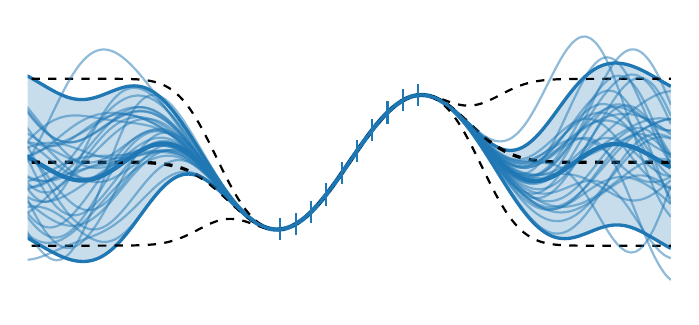
\begin{tikzpicture}
\begin{axis}[axis lines={none}, height={5cm}, width={9.75cm}, xmin={-0.15}, xmax={1.25}, ymin={-1}, ymax={1}]
    \node at (-0.15,-1) {};
    \node at (-0.15,1) {};
    \node at (1.25,1) {};
    \node at (1.25,-1) {};
    \addplot[no markers, smooth, very thick, color={rgb,1:red,0.1216;green,0.4667;blue,0.7059}, name path={upper}]
        coordinates {
            (-0.25,0.7475199970486859)
            (-0.2375,0.743635584221933)
            (-0.225,0.7369619008113851)
            (-0.2125,0.7274538617768901)
            (-0.2,0.7151208163745069)
            (-0.1875,0.7000345745072851)
            (-0.175,0.6823355541143689)
            (-0.1625,0.6622417296565598)
            (-0.15,0.6400649088515606)
            (-0.1375,0.6162357097529717)
            (-0.125,0.5913332167750793)
            (-0.1125,0.5661096041610034)
            (-0.1,0.5414962991434547)
            (-0.0875,0.5185782290800787)
            (-0.075,0.4985270961223992)
            (-0.0625,0.4824931928073868)
            (-0.05,0.47146664943444505)
            (-0.0375,0.4661303215356922)
            (-0.025,0.4667335129734085)
            (-0.0125,0.473014360043165)
            (0.0,0.4841880660679918)
            (0.0125,0.4990021107479401)
            (0.025,0.5158447614360953)
            (0.0375,0.5328849721848778)
            (0.05,0.5482211289699919)
            (0.0625,0.5600205874167281)
            (0.075,0.5666381414619841)
            (0.0875,0.5667071333336138)
            (0.1,0.5592010376554191)
            (0.1125,0.5434661359110465)
            (0.125,0.5192277444776872)
            (0.1375,0.4865737069202311)
            (0.15,0.4459196884311217)
            (0.1625,0.3979612790379965)
            (0.175,0.34361802947283526)
            (0.1875,0.2839743156686624)
            (0.2,0.22022138268785293)
            (0.2125,0.1536041141248859)
            (0.225,0.0853750945607405)
            (0.2375,0.016757477490185108)
            (0.25,-0.051082857423525925)
            (0.2625,-0.11705628552268472)
            (0.275,-0.1801607054500738)
            (0.2875,-0.23948672875866814)
            (0.3,-0.2942186568735372)
            (0.3125,-0.3436331015851756)
            (0.325,-0.3870968894171206)
            (0.3375,-0.4240655220686292)
            (0.35,-0.45408301003314294)
            (0.3625,-0.47678341780661865)
            (0.375,-0.49189401912137193)
            (0.3875,-0.4992395985860357)
            (0.4,-0.49874553876918476)
            (0.4125,-0.4904335266860326)
            (0.425,-0.474486167595979)
            (0.4375,-0.4511322689145864)
            (0.45,-0.42073363055439983)
            (0.4625,-0.38376996631209387)
            (0.475,-0.3408172394208204)
            (0.4875,-0.2925460385066784)
            (0.5,-0.23971057368572912)
            (0.5125,-0.18313467777587317)
            (0.525,-0.12370059296282165)
            (0.5375,-0.062335913855344226)
            (0.55,1.7360655865627565e-6)
            (0.5625,0.062339531348626936)
            (0.575,0.12370424576775765)
            (0.5875,0.18313817566466628)
            (0.6,0.23971437233040904)
            (0.6125,0.2925501044389145)
            (0.625,0.3408208841610769)
            (0.6375,0.38377436033105417)
            (0.65,0.42073941499043366)
            (0.6625,0.4511363736060366)
            (0.675,0.47449500606303335)
            (0.6875,0.49045123106727895)
            (0.7,0.4987494587420837)
            (0.7125,0.4993459980538318)
            (0.725,0.49231004184709437)
            (0.7375,0.47790260255820977)
            (0.75,0.4565842902621308)
            (0.7625,0.42902693725809676)
            (0.775,0.39612124459495035)
            (0.7875,0.3589761671088359)
            (0.8,0.3189075374334771)
            (0.8125,0.27741389116415366)
            (0.825,0.23613822573995127)
            (0.8375,0.1968154853338575)
            (0.85,0.16120683173510247)
            (0.8625,0.13102313513632935)
            (0.875,0.10784146725088767)
            (0.8875,0.09301955989206402)
            (0.9,0.087614067157998)
            (0.9125,0.09230891599434038)
            (0.925,0.10735995695102907)
            (0.9375,0.13256148879096818)
            (0.95,0.16723902894361742)
            (0.9625,0.210270993659406)
            (0.975,0.26013984423956615)
            (0.9875,0.31501089570356305)
            (1.0,0.3728345491072598)
            (1.0125,0.43146538513826954)
            (1.025,0.48878953239931766)
            (1.0375,0.5428501791023767)
            (1.05,0.5919602146736098)
            (1.0625,0.6347909903918662)
            (1.075,0.6704273840320658)
            (1.0875,0.6983821631323543)
            (1.1,0.7185674963328151)
            (1.1125,0.7312284396896196)
            (1.125,0.7368514017635815)
            (1.1375,0.7360674943373565)
            (1.15,0.729572700519693)
            (1.1625,0.7180812213514547)
            (1.175,0.7023160247999477)
            (1.1875,0.6830265932594178)
            (1.2,0.6610146623343041)
            (1.2125,0.637148076271076)
            (1.225,0.6123497820879645)
            (1.2375,0.5875594281200807)
            (1.25,0.5636748385082125)
        }
        ;
    \addplot[no markers, smooth, very thick, color={rgb,1:red,0.1216;green,0.4667;blue,0.7059}, name path={lower}]
        coordinates {
            (-0.25,-0.46335543594499207)
            (-0.2375,-0.46598291181443463)
            (-0.225,-0.471252272489911)
            (-0.2125,-0.4793432630650575)
            (-0.2,-0.4904080223867582)
            (-0.1875,-0.5045208561469254)
            (-0.175,-0.5216248244420375)
            (-0.1625,-0.5414870999748967)
            (-0.15,-0.5636748519531707)
            (-0.1375,-0.5875594391918649)
            (-0.125,-0.6123497902934316)
            (-0.1125,-0.6371480815180388)
            (-0.1,-0.6610146647706412)
            (-0.0875,-0.6830265931941155)
            (-0.075,-0.7023160225142934)
            (-0.0625,-0.7180812170316715)
            (-0.05,-0.7295726942961787)
            (-0.0375,-0.7360674865012327)
            (-0.025,-0.7368513929867533)
            (-0.0125,-0.7312284312891809)
            (0.0,-0.7185674904019435)
            (0.0125,-0.6983821625331097)
            (0.025,-0.6704273921601029)
            (0.0375,-0.634791010845664)
            (0.05,-0.591960250828599)
            (0.0625,-0.5428502336702772)
            (0.075,-0.48878960707528085)
            (0.0875,-0.43146548037137783)
            (0.1,-0.37283466397835857)
            (0.1125,-0.3150110279464685)
            (0.125,-0.2601399904424378)
            (0.1375,-0.21027114947114572)
            (0.15,-0.1672391894832293)
            (0.1625,-0.13256164905841294)
            (0.175,-0.10736011211933705)
            (0.1875,-0.09230906173984443)
            (0.2,-0.08761419996763162)
            (0.2125,-0.093019677268029)
            (0.225,-0.10784156777800463)
            (0.2375,-0.13102321837064038)
            (0.25,-0.1612068982422531)
            (0.2625,-0.19681553642650734)
            (0.275,-0.23613826329796384)
            (0.2875,-0.27741391739715016)
            (0.3,-0.31890755469581444)
            (0.3125,-0.35897617764532513)
            (0.325,-0.3961212503785013)
            (0.3375,-0.4290269399545125)
            (0.35,-0.45658429127073147)
            (0.3625,-0.4779026026917245)
            (0.375,-0.4923100417355956)
            (0.3875,-0.4993459979492)
            (0.4,-0.49874945872582593)
            (0.4125,-0.4904512310381083)
            (0.425,-0.4744950060419391)
            (0.4375,-0.4511363735395029)
            (0.45,-0.42073941487191235)
            (0.4625,-0.3837743604737161)
            (0.475,-0.3408208842716168)
            (0.4875,-0.2925501046612241)
            (0.5,-0.23971437235462434)
            (0.5125,-0.18313817576851438)
            (0.525,-0.12370424561603754)
            (0.5375,-0.06233953154515435)
            (0.55,-1.7360742267624233e-6)
            (0.5625,0.06233591392408763)
            (0.575,0.12370059276426257)
            (0.5875,0.1831346778854056)
            (0.6,0.23971057366151383)
            (0.6125,0.29254603893999076)
            (0.625,0.34081723963208677)
            (0.6375,0.3837699665334271)
            (0.65,0.4207336304701551)
            (0.6625,0.4511322688772134)
            (0.675,0.47448616758088175)
            (0.6875,0.49043352663690987)
            (0.7,0.49874553875824185)
            (0.7125,0.499239598521308)
            (0.725,0.4918940190875497)
            (0.7375,0.4767834179272868)
            (0.75,0.45408301067430773)
            (0.7625,0.4240655236804725)
            (0.775,0.38709689274196635)
            (0.7875,0.34363310746209613)
            (0.8,0.2942186662607873)
            (0.8125,0.23948674269506895)
            (0.825,0.18016072494040566)
            (0.8375,0.1170563114144869)
            (0.85,0.051082890288922274)
            (0.8625,-0.01675743744800484)
            (0.875,-0.08537504759564235)
            (0.8875,-0.15360406103351276)
            (0.9,-0.22022132476402353)
            (0.9125,-0.28397425469059406)
            (0.925,-0.3436179675817639)
            (0.9375,-0.39796121860226086)
            (0.95,-0.4459196318138987)
            (0.9625,-0.4865736563030218)
            (0.975,-0.5192277016421853)
            (0.9875,-0.5434661020139064)
            (1.0,-0.5592010131401177)
            (1.0125,-0.5667071178270384)
            (1.025,-0.566638133813052)
            (1.0375,-0.5600205858018829)
            (1.05,-0.5482211311113234)
            (1.0625,-0.532884975628167)
            (1.075,-0.5158447638993513)
            (1.0875,-0.49900211044962717)
            (1.1,-0.48418806200840525)
            (1.1125,-0.47301435218058785)
            (1.125,-0.4667335021932585)
            (1.1375,-0.46613030946689926)
            (1.15,-0.4714666380797006)
            (1.1625,-0.4824931841265685)
            (1.175,-0.498527091584399)
            (1.1875,-0.5185782294475464)
            (1.2,-0.5414963043671661)
            (1.2125,-0.5661096134885795)
            (1.225,-0.5913332289299017)
            (1.2375,-0.6162357233333255)
            (1.25,-0.6400649225174032)
        }
        ;
    \addplot[color={rgb,1:red,0.1216;green,0.4667;blue,0.7059}, opacity={0.25}]
        fill between [of = upper and lower]
        ;
    \addplot[no markers, smooth, ultra thick, color={rgb,1:red,0.1216;green,0.4667;blue,0.7059}]
        coordinates {
            (-0.25,0.1420822805518469)
            (-0.2375,0.13882633620374918)
            (-0.225,0.13285481416073708)
            (-0.2125,0.1240552993559163)
            (-0.2,0.11235639699387434)
            (-0.1875,0.09775685918017984)
            (-0.175,0.08035536483616568)
            (-0.1625,0.06037731484083153)
            (-0.15,0.03819502844919498)
            (-0.1375,0.014338135280553388)
            (-0.125,-0.010508286759176144)
            (-0.1125,-0.035519238678517695)
            (-0.1,-0.05975918281359327)
            (-0.0875,-0.08222418205701842)
            (-0.075,-0.10189446319594708)
            (-0.0625,-0.11779401211214235)
            (-0.05,-0.1290530224308668)
            (-0.0375,-0.13496858248277022)
            (-0.025,-0.1350589400066724)
            (-0.0125,-0.12910703562300796)
            (0.0,-0.11718971216697582)
            (0.0125,-0.0996900258925848)
            (0.025,-0.07729131536200384)
            (0.0375,-0.05095301933039309)
            (0.05,-0.02186956092930359)
            (0.0625,0.008585176873225464)
            (0.075,0.038924267193351625)
            (0.0875,0.067620826481118)
            (0.1,0.09318318683853022)
            (0.1125,0.11422755398228901)
            (0.125,0.1295438770176247)
            (0.1375,0.1381512787245427)
            (0.15,0.1393402494739462)
            (0.1625,0.13269981498979178)
            (0.175,0.11812895867674911)
            (0.1875,0.09583262696440897)
            (0.2,0.06630359136011066)
            (0.2125,0.03029221842842844)
            (0.225,-0.011233236608632069)
            (0.2375,-0.057132870440227634)
            (0.25,-0.1061448778328895)
            (0.2625,-0.15693591097459603)
            (0.275,-0.2081494843740188)
            (0.2875,-0.25845032307790916)
            (0.3,-0.3065631057846758)
            (0.3125,-0.3513046396152504)
            (0.325,-0.39160906989781097)
            (0.3375,-0.42654623101157085)
            (0.35,-0.4553336506519372)
            (0.3625,-0.4773430102491716)
            (0.375,-0.49210203042848377)
            (0.3875,-0.49929279826761785)
            (0.4,-0.49874749874750535)
            (0.4125,-0.4904423788620704)
            (0.425,-0.47449058681895906)
            (0.4375,-0.45113432122704467)
            (0.45,-0.4207365227131561)
            (0.4625,-0.383772163392905)
            (0.475,-0.3408190618462186)
            (0.4875,-0.29254807158395124)
            (0.5,-0.23971247302017673)
            (0.5125,-0.18313642677219377)
            (0.525,-0.1237024192894296)
            (0.5375,-0.06233772270024929)
            (0.55,-4.320099833421409e-12)
            (0.5625,0.062337722636357285)
            (0.575,0.12370241926601011)
            (0.5875,0.18313642677503594)
            (0.6,0.23971247299596143)
            (0.6125,0.2925480716894526)
            (0.625,0.34081906189658184)
            (0.6375,0.38377216343224063)
            (0.65,0.4207365227302944)
            (0.6625,0.451134321241625)
            (0.675,0.47449058682195755)
            (0.6875,0.4904423788520944)
            (0.7,0.4987474987501628)
            (0.7125,0.4992927982875699)
            (0.725,0.49210203046732204)
            (0.7375,0.4773430102427483)
            (0.75,0.4553336504682193)
            (0.7625,0.42654623046928464)
            (0.775,0.39160906866845835)
            (0.7875,0.351304637285466)
            (0.8,0.3065631018471322)
            (0.8125,0.2584503169296113)
            (0.825,0.20814947534017847)
            (0.8375,0.1569358983741722)
            (0.85,0.10614486101201237)
            (0.8625,0.057132848844162254)
            (0.875,0.011233209827622659)
            (0.8875,-0.030292250570724377)
            (0.9,-0.06630362880301277)
            (0.9125,-0.09583266934812684)
            (0.925,-0.11812900531536741)
            (0.9375,-0.13269986490564634)
            (0.95,-0.13934030143514065)
            (0.9625,-0.1381513313218079)
            (0.975,-0.1295439287013096)
            (0.9875,-0.11422760315517166)
            (1.0,-0.09318323201642897)
            (1.0125,-0.06762086634438447)
            (1.025,-0.03892430070686714)
            (1.0375,-0.008585203349753101)
            (1.05,0.021869541781143198)
            (1.0625,0.0509530073818496)
            (1.075,0.07729131006635725)
            (1.0875,0.09969002634136359)
            (1.1,0.11718971716220494)
            (1.1125,0.12910704375451587)
            (1.125,0.13505894978516153)
            (1.1375,0.13496859243522863)
            (1.15,0.12905303121999623)
            (1.1625,0.1177940186124431)
            (1.175,0.10189446660777435)
            (1.1875,0.08222418190593572)
            (1.2,0.05975917898356897)
            (1.2125,0.03551923139124824)
            (1.225,0.010508276579031417)
            (1.2375,-0.014338147606622442)
            (1.25,-0.038195042004595336)
        }
        ;
    \addplot[no markers, smooth, thick, dashed]
        coordinates {
            (-0.25,0.61980642300806)
            (-0.2375,0.6198064248612742)
            (-0.225,0.6198064287088184)
            (-0.2125,0.6198064365481787)
            (-0.2,0.6198064522193969)
            (-0.1875,0.6198064829464042)
            (-0.175,0.6198065420187121)
            (-0.1625,0.6198066533251091)
            (-0.15,0.6198068587834313)
            (-0.1375,0.6198072301032942)
            (-0.125,0.6198078866874375)
            (-0.1125,0.6198090216146855)
            (-0.1,0.6198109371219708)
            (-0.0875,0.6198140889920313)
            (-0.075,0.6198191342720151)
            (-0.0625,0.619826966210793)
            (-0.05,0.6198386998471443)
            (-0.0375,0.6198555342109099)
            (-0.025,0.6198783516731907)
            (-0.0125,0.6199068061313036)
            (0.0,0.6199374806869269)
            (0.0125,0.6199604462490093)
            (0.025,0.6199532266120523)
            (0.0375,0.6198708192106269)
            (0.05,0.6196301619887266)
            (0.0625,0.6190875175987273)
            (0.075,0.6180080139434109)
            (0.0875,0.6160283901163536)
            (0.1,0.6126169947105218)
            (0.1125,0.6070389165388889)
            (0.125,0.5983377535545278)
            (0.1375,0.5853473500466616)
            (0.15,0.5667452815285409)
            (0.1625,0.5411541817374976)
            (0.175,0.5072877882445361)
            (0.1875,0.4641277334795479)
            (0.2,0.4111072227031115)
            (0.2125,0.3482713563427175)
            (0.225,0.2763828776272344)
            (0.2375,0.19694749285686475)
            (0.25,0.11214436103822056)
            (0.2625,0.024663285895479226)
            (0.275,-0.06253230826528239)
            (0.2875,-0.14648212027659535)
            (0.3,-0.224501477299836)
            (0.3125,-0.294404992943187)
            (0.325,-0.3546458524389714)
            (0.3375,-0.4043524500455471)
            (0.35,-0.4432656187698042)
            (0.3625,-0.47160014071141476)
            (0.375,-0.48986832972788996)
            (0.3875,-0.4987076167030337)
            (0.4,-0.49874553333870664)
            (0.4125,-0.4903371288133945)
            (0.425,-0.47444902800608735)
            (0.4375,-0.45112214147752877)
            (0.45,-0.420715963714763)
            (0.4625,-0.3837661919791957)
            (0.475,-0.34081141854375036)
            (0.4875,-0.29254057591516724)
            (0.5,-0.23971080711024592)
            (0.5125,-0.18313089481662967)
            (0.525,-0.12369797265732008)
            (0.5375,-0.06233472446227518)
            (0.55,4.9533438610480414e-6)
            (0.5625,0.062339984957248525)
            (0.575,0.12370610831569977)
            (0.5875,0.1831418896120811)
            (0.6,0.23971472694450305)
            (0.6125,0.2925560749287241)
            (0.625,0.34082660137746673)
            (0.6375,0.38377796010413967)
            (0.65,0.4207578800123561)
            (0.6625,0.45114741510084283)
            (0.675,0.47452854757378626)
            (0.6875,0.4905360905064382)
            (0.7,0.4987494533769682)
            (0.7125,0.49998142379092586)
            (0.725,0.49479283904528015)
            (0.7375,0.4844282698493996)
            (0.75,0.47059283345522873)
            (0.7625,0.455330770550934)
            (0.775,0.4408289292243682)
            (0.7875,0.4291717370359268)
            (0.8,0.4220902783048156)
            (0.8125,0.4207521803102541)
            (0.825,0.42563190343076396)
            (0.8375,0.43648469388838024)
            (0.85,0.45242625960352073)
            (0.8625,0.47209952966394164)
            (0.875,0.4938944588081274)
            (0.8875,0.5161797732275798)
            (0.9,0.5375075254393237)
            (0.9125,0.5567608579130806)
            (0.925,0.5732295059120482)
            (0.9375,0.5866127817293189)
            (0.95,0.5969628589860081)
            (0.9625,0.6045897922946819)
            (0.975,0.6099527212617755)
            (0.9875,0.6135592311600455)
            (1.0,0.6158881709918762)
            (1.0125,0.6173425675455537)
            (1.025,0.6182311545064509)
            (1.0375,0.6187715027362417)
            (1.05,0.6191056544562508)
            (1.0625,0.6193200663344255)
            (1.075,0.6194642453898833)
            (1.0875,0.61956531915836)
            (1.1,0.6196379914653521)
            (1.1125,0.6196905890609122)
            (1.125,0.6197283390533027)
            (1.1375,0.6197549473896921)
            (1.15,0.6197732693527331)
            (1.1625,0.6197855649311347)
            (1.175,0.6197936012889854)
            (1.1875,0.6197987182047101)
            (1.2,0.6198018942661385)
            (1.2125,0.6198038176483757)
            (1.225,0.6198049550474513)
            (1.2375,0.6198056123799179)
            (1.25,0.6198059839183423)
        }
        ;
    \addplot[no markers, smooth, thick, dashed]
        coordinates {
            (-0.25,-0.6198064197779438)
            (-0.2375,-0.6198064179247262)
            (-0.225,-0.6198064140771674)
            (-0.2125,-0.6198064062377425)
            (-0.2,-0.6198063905662512)
            (-0.1875,-0.6198063598381282)
            (-0.175,-0.6198063007614204)
            (-0.1625,-0.6198061894382682)
            (-0.15,-0.6198059839183503)
            (-0.1375,-0.6198056123799331)
            (-0.125,-0.6198049550474798)
            (-0.1125,-0.6198038176484283)
            (-0.1,-0.6198018942662337)
            (-0.0875,-0.6197987182048789)
            (-0.075,-0.6197936012892801)
            (-0.0625,-0.61978556493164)
            (-0.05,-0.6197732693535853)
            (-0.0375,-0.6197549473911056)
            (-0.025,-0.619728339055611)
            (-0.0125,-0.6196905890646263)
            (0.0,-0.6196379914712475)
            (0.0125,-0.6195653191676077)
            (0.025,-0.6194642454042433)
            (0.0375,-0.6193200663565387)
            (0.05,-0.6191056544900688)
            (0.0625,-0.6187715027876385)
            (0.075,-0.6182311545840545)
            (0.0875,-0.6173425676617986)
            (0.1,-0.6158881711641773)
            (0.1125,-0.6135592314119468)
            (0.125,-0.6099527216237357)
            (0.1375,-0.6045897928040641)
            (0.15,-0.5969628596859405)
            (0.1625,-0.5866127826659657)
            (0.175,-0.5732295071301579)
            (0.1875,-0.5567608594504083)
            (0.2,-0.5375075273197141)
            (0.2125,-0.5161797754539079)
            (0.225,-0.4938944613578103)
            (0.2375,-0.47209953248444647)
            (0.25,-0.45242626261260077)
            (0.2625,-0.43648469698101977)
            (0.275,-0.42563190648430554)
            (0.2875,-0.42075218319671626)
            (0.3,-0.4220902809103702)
            (0.3125,-0.4291717392684752)
            (0.325,-0.4408289310211695)
            (0.3375,-0.45533077189916205)
            (0.35,-0.470592834383468)
            (0.3625,-0.4844282704093502)
            (0.375,-0.49479283933327933)
            (0.3875,-0.4999814238948806)
            (0.4,-0.4987494533769493)
            (0.4125,-0.4905360905103863)
            (0.425,-0.47452854750831786)
            (0.4375,-0.45114741501665573)
            (0.45,-0.42075788000704467)
            (0.4625,-0.38377796013336773)
            (0.475,-0.34082660114475244)
            (0.4875,-0.29255607490183666)
            (0.5,-0.23971472693088094)
            (0.5125,-0.18314188975767667)
            (0.525,-0.12370610829602124)
            (0.5375,-0.06233998497797066)
            (0.55,-4.95334356972552e-6)
            (0.5625,0.06233472448209137)
            (0.575,0.12369797263768063)
            (0.5875,0.18313089496196944)
            (0.6,0.23971080709666645)
            (0.6125,0.2925405758870186)
            (0.625,0.3408114183059379)
            (0.6375,0.38376619200433104)
            (0.65,0.42071596370481174)
            (0.6625,0.4511221413887427)
            (0.675,0.47444902794015)
            (0.6875,0.49033712881909275)
            (0.7,0.4987455333387255)
            (0.7125,0.4987076167978817)
            (0.725,0.4898683299840073)
            (0.7375,0.47160014119924254)
            (0.75,0.4432656195650604)
            (0.7625,0.40435245117942314)
            (0.775,0.3546458539212535)
            (0.7875,0.2944049947478814)
            (0.8,0.22450147935918252)
            (0.8125,0.14648212250197723)
            (0.825,0.06253231055525724)
            (0.8375,-0.024663283648010792)
            (0.85,-0.11214435892929125)
            (0.8625,-0.19694749096183495)
            (0.875,-0.27638287599798145)
            (0.8875,-0.34827135500379025)
            (0.9,-0.4111072216535917)
            (0.9125,-0.4641277326986385)
            (0.925,-0.5072877876968729)
            (0.9375,-0.5411541813800415)
            (0.95,-0.5667452813166778)
            (0.9625,-0.5853473499388024)
            (0.975,-0.5983377535152861)
            (0.9875,-0.6070389165405374)
            (1.0,-0.6126169947330691)
            (1.0125,-0.6160283901466395)
            (1.025,-0.6180080139736868)
            (1.0375,-0.6190875176251209)
            (1.05,-0.6196301620098668)
            (1.0625,-0.6198708192265677)
            (1.075,-0.619953226623525)
            (1.0875,-0.6199604462569587)
            (1.1,-0.6199374806922612)
            (1.1125,-0.6199068061347842)
            (1.125,-0.6198783516754057)
            (1.1375,-0.6198555342122877)
            (1.15,-0.6198386998479832)
            (1.1625,-0.6198269662112935)
            (1.175,-0.619819134272308)
            (1.1875,-0.6198140889921996)
            (1.2,-0.6198109371220657)
            (1.2125,-0.6198090216147382)
            (1.225,-0.619807886687466)
            (1.2375,-0.6198072301033094)
            (1.25,-0.6198068587834393)
        }
        ;
    \addplot[no markers, smooth, very thick, dashed]
        coordinates {
            (-0.25,1.615058070458892e-9)
            (-0.2375,3.468273969598577e-9)
            (-0.225,7.315825471177542e-9)
            (-0.2125,1.5155218054216632e-8)
            (-0.2,3.082657280029257e-8)
            (-0.1875,6.155413796212785e-8)
            (-0.175,1.2062864583890434e-7)
            (-0.1625,2.3194342043361265e-7)
            (-0.15,4.374325405155705e-7)
            (-0.1375,8.088616804814171e-7)
            (-0.125,1.4658199787911873e-6)
            (-0.1125,2.601983128635646e-6)
            (-0.1,4.521427868575746e-6)
            (-0.0875,7.685393576246203e-6)
            (-0.075,1.2766491367461039e-5)
            (-0.0625,2.0700639576508235e-5)
            (-0.05,3.271524677952481e-5)
            (-0.0375,5.0293409902139223e-5)
            (-0.025,7.50063087898351e-5)
            (-0.0125,0.00010810853333870075)
            (0.0,0.00014974460783972923)
            (0.0125,0.00019756354070075234)
            (0.025,0.0002444906039044905)
            (0.0375,0.00027537642704413896)
            (0.05,0.000262253749328833)
            (0.0625,0.000158007405544383)
            (0.075,-0.00011157032032177895)
            (0.0875,-0.0006570887727225288)
            (0.1,-0.001635588226827718)
            (0.1125,-0.0032601574365289736)
            (0.125,-0.005807484034603981)
            (0.1375,-0.009621221378701202)
            (0.15,-0.015108789078699825)
            (0.1625,-0.022729300464234055)
            (0.175,-0.032970859442810904)
            (0.1875,-0.04631656298543023)
            (0.2,-0.06320015230830128)
            (0.2125,-0.08395420955559518)
            (0.225,-0.10875579186528796)
            (0.2375,-0.13757601981379086)
            (0.25,-0.1701409507871901)
            (0.2625,-0.20591070554277027)
            (0.275,-0.24408210737479397)
            (0.2875,-0.2836171517366558)
            (0.3,-0.3232958791051031)
            (0.3125,-0.3617883661058311)
            (0.325,-0.39773739173007044)
            (0.3375,-0.42984161097235457)
            (0.35,-0.4569292265766361)
            (0.3625,-0.4780142055603825)
            (0.375,-0.49233058453058465)
            (0.3875,-0.49934452029895715)
            (0.4,-0.498747493357828)
            (0.4125,-0.4904366096618904)
            (0.425,-0.4744887877572026)
            (0.4375,-0.45113477824709225)
            (0.45,-0.42073692186090383)
            (0.4625,-0.3837720760562817)
            (0.475,-0.3408190098442514)
            (0.4875,-0.29254832540850195)
            (0.5,-0.23971276702056343)
            (0.5125,-0.18313639228715317)
            (0.525,-0.12370204047667066)
            (0.5375,-0.06233735472012292)
            (0.55,1.4566126083082054e-13)
            (0.5625,0.062337354719669946)
            (0.575,0.1237020404766902)
            (0.5875,0.18313639228702527)
            (0.6,0.23971276702058475)
            (0.6125,0.29254832540787135)
            (0.625,0.3408190098417023)
            (0.6375,0.38377207605423536)
            (0.65,0.4207369218585839)
            (0.6625,0.45113477824479276)
            (0.675,0.4744887877569681)
            (0.6875,0.4904366096627655)
            (0.7,0.49874749335784685)
            (0.7125,0.4993445202944038)
            (0.725,0.49233058451464373)
            (0.7375,0.47801420552432106)
            (0.75,0.45692922651014456)
            (0.7625,0.4298416108651786)
            (0.775,0.39773739157281085)
            (0.7875,0.3617883658919041)
            (0.8,0.32329587883199906)
            (0.8125,0.28361715140611565)
            (0.825,0.24408210699301058)
            (0.8375,0.20591070512018472)
            (0.85,0.17014095033711474)
            (0.8625,0.13757601935105335)
            (0.875,0.10875579140507297)
            (0.8875,0.08395420911189477)
            (0.9,0.06320015189286599)
            (0.9125,0.04631656260722106)
            (0.925,0.03297085910758768)
            (0.9375,0.0227293001746387)
            (0.95,0.015108788834665099)
            (0.9625,0.009621221177939676)
            (0.975,0.0058074838732447565)
            (0.9875,0.0032601573097540415)
            (1.0,0.0016355881294036062)
            (1.0125,0.0006570886994571451)
            (1.025,0.00011157026638212997)
            (1.0375,-0.00015800744443956322)
            (1.05,-0.0002622537768080368)
            (1.0625,-0.0002753764460711218)
            (1.075,-0.00024449061682089036)
            (1.0875,-0.00019756354929934428)
            (1.1,-0.00014974461345451163)
            (1.1125,-0.0001081085369359486)
            (1.125,-7.50063110514806e-5)
            (1.1375,-5.02934112977937e-5)
            (1.15,-3.271524762503205e-5)
            (1.1625,-2.0700640079441505e-5)
            (1.175,-1.2766491661241294e-5)
            (1.1875,-7.685393744793757e-6)
            (1.2,-4.521427963562827e-6)
            (1.2125,-2.6019831812254697e-6)
            (1.225,-1.4658200073992556e-6)
            (1.2375,-8.088616957736135e-7)
            (1.25,-4.3743254854877375e-7)
        }
        ;
    \addplot[no markers, smooth, thick, color={rgb,1:red,0.1216;green,0.4667;blue,0.7059}, opacity={0.5}]
        coordinates {
            (-0.25,0.1867842737814007)
            (-0.2375,0.14341925212583795)
            (-0.225,0.09948138033270917)
            (-0.2125,0.055964115649245874)
            (-0.2,0.0139590624682297)
            (-0.1875,-0.025360403578748747)
            (-0.175,-0.06077267441231146)
            (-0.1625,-0.09105699141272769)
            (-0.15,-0.11505450695507223)
            (-0.1375,-0.13173622027233167)
            (-0.125,-0.14027170223412766)
            (-0.1125,-0.1400922009296275)
            (-0.1,-0.13094207423157797)
            (-0.0875,-0.11291347388989076)
            (-0.075,-0.08646069041176294)
            (-0.0625,-0.05239239023801179)
            (-0.05,-0.011841939849452615)
            (-0.0375,0.033782089311188035)
            (-0.025,0.08286149513851829)
            (-0.0125,0.13364511995933656)
            (0.0,0.18433092132131992)
            (0.0125,0.23314756538805365)
            (0.025,0.2784300456968176)
            (0.0375,0.31868468064103006)
            (0.05,0.35264005335530213)
            (0.0625,0.37928188369638344)
            (0.075,0.397871306523694)
            (0.0875,0.4079474219380037)
            (0.1,0.4093161511595569)
            (0.1125,0.4020282798535313)
            (0.125,0.3863500445726818)
            (0.1375,0.3627297077940716)
            (0.15,0.3317633055482106)
            (0.1625,0.2941622062717783)
            (0.175,0.25072438300009464)
            (0.1875,0.20231047727692533)
            (0.2,0.14982492547163767)
            (0.2125,0.09420171702527125)
            (0.225,0.03639382734023495)
            (0.2375,-0.022634944439965006)
            (0.25,-0.08191709110034692)
            (0.2625,-0.14048870831476692)
            (0.275,-0.1973979630016466)
            (0.2875,-0.25171529630282846)
            (0.3,-0.3025455123809602)
            (0.3125,-0.349041499944865)
            (0.325,-0.3904190025829502)
            (0.3375,-0.4259716334857214)
            (0.35,-0.4550852371164357)
            (0.3625,-0.47725073254390066)
            (0.375,-0.49207471157521965)
            (0.3875,-0.49928727743087675)
            (0.4,-0.49874685767240595)
            (0.4125,-0.4904419695407801)
            (0.425,-0.4744901229093364)
            (0.4375,-0.4511341917340036)
            (0.45,-0.42073665776314423)
            (0.4625,-0.38377213323474474)
            (0.475,-0.34081851372947614)
            (0.4875,-0.292547022995675)
            (0.5,-0.23971131070142837)
            (0.5125,-0.18313567970212363)
            (0.525,-0.12370246730821549)
            (0.5375,-0.06233860008491479)
            (0.55,-1.378406461138848e-6)
            (0.5625,0.06233637852201171)
            (0.575,0.12370160799184832)
            (0.5875,0.1831363973772518)
            (0.6,0.23971314044313158)
            (0.6125,0.29254909732625056)
            (0.625,0.34082005237190927)
            (0.6375,0.38377287553613215)
            (0.65,0.4207369482299299)
            (0.6625,0.4511345867236689)
            (0.675,0.4744907554091249)
            (0.6875,0.4904424696074604)
            (0.7,0.49874831028197)
            (0.7125,0.49929838780514413)
            (0.725,0.4921248855396776)
            (0.7375,0.47741299767088113)
            (0.75,0.4555116740749674)
            (0.7625,0.42694314516068455)
            (0.775,0.39240978158990614)
            (0.7875,0.3527965142668762)
            (0.8,0.3091668669954362)
            (0.8125,0.26275069319741307)
            (0.825,0.21492199801208806)
            (0.8375,0.1671657783233101)
            (0.85,0.12103360694848492)
            (0.8625,0.07808867106748871)
            (0.875,0.03984206775210203)
            (0.8875,0.007683256977300518)
            (0.9,-0.017191442650829336)
            (0.9125,-0.03384767579971133)
            (0.925,-0.04167413122038451)
            (0.9375,-0.04043081849610691)
            (0.95,-0.030279930805403907)
            (0.9625,-0.011795592623461582)
            (0.975,0.014049892469337633)
            (0.9875,0.04592404872675426)
            (1.0,0.0821954318789396)
            (1.0125,0.12101513294154781)
            (1.025,0.16041398915743116)
            (1.0375,0.19840951611853552)
            (1.05,0.23311562447613537)
            (1.0625,0.26284777652455166)
            (1.075,0.2862164233718646)
            (1.0875,0.30220233756712067)
            (1.1,0.3102087576598288)
            (1.1125,0.31008697812628866)
            (1.125,0.3021339983278728)
            (1.1375,0.28706291098845227)
            (1.15,0.2659486806472128)
            (1.1625,0.2401536644202366)
            (1.175,0.21123851943302185)
            (1.1875,0.18086492497107207)
            (1.2,0.1506967773779896)
            (1.2125,0.12230620218334554)
            (1.225,0.09708993425855825)
            (1.2375,0.07620045092598446)
            (1.25,0.0604948426028807)
        }
        ;
    \addplot[no markers, smooth, thick, color={rgb,1:red,0.1216;green,0.4667;blue,0.7059}, opacity={0.5}]
        coordinates {
            (-0.25,0.05355803210972518)
            (-0.2375,0.11026763553416584)
            (-0.225,0.1576154784847842)
            (-0.2125,0.19451659988696204)
            (-0.2,0.22027790272027037)
            (-0.1875,0.2346211139699089)
            (-0.175,0.23768960762254931)
            (-0.1625,0.2300389612440958)
            (-0.15,0.21261160660366235)
            (-0.1375,0.18669641727484748)
            (-0.125,0.15387455584400797)
            (-0.1125,0.11595338943984389)
            (-0.1,0.07489076681171865)
            (-0.0875,0.03271241950190423)
            (-0.075,-0.008574320194650986)
            (-0.0625,-0.04706694028684716)
            (-0.05,-0.08105052993540052)
            (-0.0375,-0.10907306555247541)
            (-0.025,-0.130009469226414)
            (-0.0125,-0.14311105094319584)
            (0.0,-0.14803752028723724)
            (0.0125,-0.14486954921990863)
            (0.025,-0.13410084871927058)
            (0.0375,-0.1166098367815865)
            (0.05,-0.09361214915145864)
            (0.0625,-0.06659639469509021)
            (0.075,-0.037246594730619254)
            (0.0875,-0.007355585437302525)
            (0.1,0.021265767604456476)
            (0.1125,0.04687844613602765)
            (0.125,0.06789925139924669)
            (0.1375,0.08297432238388824)
            (0.15,0.0910384090459056)
            (0.1625,0.09135712070744889)
            (0.175,0.08355055022479041)
            (0.1875,0.06759792916994209)
            (0.2,0.04382419623700662)
            (0.2125,0.01287046307903525)
            (0.225,-0.024348743830467943)
            (0.2375,-0.06669796254534896)
            (0.25,-0.1128791743650904)
            (0.2625,-0.16149225270809103)
            (0.275,-0.2110939357348185)
            (0.2875,-0.26025230040949915)
            (0.3,-0.3075944167651777)
            (0.3125,-0.3518456586706059)
            (0.325,-0.39185996278305824)
            (0.3375,-0.4266410829668424)
            (0.35,-0.4553555209964604)
            (0.3625,-0.47733828234915615)
            (0.375,-0.49209288358801595)
            (0.3875,-0.4992871256949474)
            (0.4,-0.49874606620312256)
            (0.4125,-0.49044340680503234)
            (0.425,-0.474492209533319)
            (0.4375,-0.45113551514973066)
            (0.45,-0.4207371111703748)
            (0.4625,-0.3837724197635582)
            (0.475,-0.3408192860094453)
            (0.4875,-0.29254834421718573)
            (0.5,-0.23971263754323693)
            (0.5125,-0.1831362365633838)
            (0.525,-0.12370173395002543)
            (0.5375,-0.06233663892902713)
            (0.55,1.1499450282281831e-6)
            (0.5625,0.062338505102717094)
            (0.575,0.12370250277357528)
            (0.5875,0.1831357568004368)
            (0.6,0.23971132568232545)
            (0.6125,0.2925469420178708)
            (0.625,0.34081841876724345)
            (0.6375,0.38377218287712656)
            (0.65,0.42073695679267437)
            (0.6625,0.45113464000949477)
            (0.675,0.47449041475222764)
            (0.6875,0.4904420239438525)
            (0.7,0.49874805359543517)
            (0.7125,0.49929491154843075)
            (0.725,0.49210206839611126)
            (0.7375,0.47732502965236645)
            (0.75,0.45525547869425387)
            (0.7625,0.42631808038199537)
            (0.775,0.3910635741886714)
            (0.7875,0.3501580098469438)
            (0.8,0.30436826421834656)
            (0.8125,0.2545442973372186)
            (0.825,0.2015989130698944)
            (0.8375,0.14648604468795698)
            (0.85,0.09017874325358499)
            (0.8625,0.033648076027983836)
            (0.875,-0.022155975109724058)
            (0.8875,-0.0763207883166449)
            (0.9,-0.127984108497006)
            (0.9125,-0.17634381222466397)
            (0.925,-0.2206649475722684)
            (0.9375,-0.2602850103327769)
            (0.95,-0.2946187480523686)
            (0.9625,-0.32316393613078165)
            (0.975,-0.34550950012130643)
            (0.9875,-0.36134704559708586)
            (1.0,-0.37048631001322857)
            (1.0125,-0.37287431293607165)
            (1.025,-0.36861712368132193)
            (1.0375,-0.3580022857920288)
            (1.05,-0.3415191492096469)
            (1.0625,-0.31987377843007736)
            (1.075,-0.293994833940252)
            (1.0875,-0.26502694560561124)
            (1.1,-0.234308655038884)
            (1.1125,-0.20333299821090106)
            (1.125,-0.17369017937950088)
            (1.1375,-0.14699345307084216)
            (1.15,-0.12479114004330807)
            (1.1625,-0.10846948300741827)
            (1.175,-0.09915261075439417)
            (1.1875,-0.09760704099803515)
            (1.2,-0.10415875387440124)
            (1.2125,-0.11863079201953916)
            (1.225,-0.1403085304717096)
            (1.2375,-0.1679382215320502)
            (1.25,-0.19976223544309216)
        }
        ;
    \addplot[no markers, smooth, thick, color={rgb,1:red,0.1216;green,0.4667;blue,0.7059}, opacity={0.5}]
        coordinates {
            (-0.25,-0.44349722181828105)
            (-0.2375,-0.5075271558216733)
            (-0.225,-0.5660250268904163)
            (-0.2125,-0.6168508747575291)
            (-0.2,-0.6584367059400703)
            (-0.1875,-0.689869856867924)
            (-0.175,-0.7109184814437568)
            (-0.1625,-0.721998689923715)
            (-0.15,-0.7240882678638639)
            (-0.1375,-0.7185967255491303)
            (-0.125,-0.7072052169303962)
            (-0.1125,-0.6916922716251657)
            (-0.1,-0.6737621052844218)
            (-0.0875,-0.6548914703773493)
            (-0.075,-0.6362087000461402)
            (-0.0625,-0.6184150525981407)
            (-0.05,-0.601754061811338)
            (-0.0375,-0.5860297949842075)
            (-0.025,-0.5706701976892112)
            (-0.0125,-0.5548275189889358)
            (0.0,-0.5375045496418038)
            (0.0125,-0.5176933542890454)
            (0.025,-0.4945124860901052)
            (0.0375,-0.4673293529442439)
            (0.05,-0.4358563316817261)
            (0.0625,-0.4002121595749682)
            (0.075,-0.3609437392052789)
            (0.0875,-0.3190073917984145)
            (0.1,-0.27571239384773993)
            (0.1125,-0.23263297035813243)
            (0.125,-0.1914974992857793)
            (0.1375,-0.1540653005866219)
            (0.15,-0.12200194322236033)
            (0.1625,-0.0967635166271103)
            (0.175,-0.07949889784014608)
            (0.1875,-0.07097690100801507)
            (0.2,-0.07154258183374196)
            (0.2125,-0.08110417320979108)
            (0.225,-0.09914943205427396)
            (0.2375,-0.12478783217681877)
            (0.25,-0.15681323760236332)
            (0.2625,-0.1937805573121421)
            (0.275,-0.23408946004086123)
            (0.2875,-0.27606848166133785)
            (0.3,-0.3180536903413166)
            (0.3125,-0.35845733464529034)
            (0.325,-0.39582341153922795)
            (0.3375,-0.4288686686021892)
            (0.35,-0.4565090282881836)
            (0.3625,-0.4778726543563356)
            (0.375,-0.4923017757302428)
            (0.3875,-0.4993458971799529)
            (0.4,-0.49874916473394915)
            (0.4125,-0.4904344626397857)
            (0.425,-0.47448637825520645)
            (0.4375,-0.4511345796013046)
            (0.45,-0.42073851031270715)
            (0.4625,-0.383773706377838)
            (0.475,-0.3408195598618503)
            (0.4875,-0.2925480290285324)
            (0.5,-0.2397126517787036)
            (0.5125,-0.18313723365941198)
            (0.525,-0.12370373219085185)
            (0.5375,-0.062339078529154116)
            (0.55,-9.350079817572673e-7)
            (0.5625,0.062337394881037275)
            (0.575,0.12370252361578946)
            (0.5875,0.18313655061655826)
            (0.6,0.23971221242973714)
            (0.6125,0.2925472643945131)
            (0.625,0.3408178877897963)
            (0.6375,0.38377106460332716)
            (0.65,0.4207359835422679)
            (0.6625,0.4511346141250285)
            (0.675,0.4744915776853365)
            (0.6875,0.4904433658844729)
            (0.7,0.49874681644650365)
            (0.7125,0.49928657654870334)
            (0.725,0.4920811135709072)
            (0.7375,0.47728669716402666)
            (0.75,0.4551987227312923)
            (0.7625,0.42624979261852486)
            (0.775,0.3910041267865988)
            (0.7875,0.35014813159587915)
            (0.8,0.3044772800261351)
            (0.8125,0.2548798090057657)
            (0.825,0.2023180606758393)
            (0.8375,0.14780853270394936)
            (0.85,0.09240180712261253)
            (0.8625,0.03716346713837099)
            (0.875,-0.016843122848317307)
            (0.8875,-0.06857169045416257)
            (0.9,-0.11700560228374136)
            (0.9125,-0.1611686549979115)
            (0.925,-0.2001351937813395)
            (0.9375,-0.23304102888665484)
            (0.95,-0.2590968023618912)
            (0.9625,-0.2776053711055716)
            (0.975,-0.287984387244153)
            (0.9875,-0.2897945801401499)
            (1.0,-0.28277332335186495)
            (1.0125,-0.26687199338674095)
            (1.025,-0.2422945149371932)
            (1.0375,-0.20953347980918885)
            (1.05,-0.1693994702552959)
            (1.0625,-0.12303884371439809)
            (1.075,-0.07193534733266801)
            (1.0875,-0.01789158356269515)
            (1.1,0.03701245818111947)
            (1.1125,0.09048491678926375)
            (1.125,0.14011070679539436)
            (1.1375,0.18346017302411505)
            (1.15,0.21821244577465548)
            (1.1625,0.2422862604446822)
            (1.175,0.2539695454025074)
            (1.1875,0.25203827639881304)
            (1.2,0.2358550745558602)
            (1.2125,0.2054388483004809)
            (1.225,0.1614984265337963)
            (1.2375,0.10542549479130253)
            (1.25,0.039245050910047645)
        }
        ;
    \addplot[no markers, smooth, thick, color={rgb,1:red,0.1216;green,0.4667;blue,0.7059}, opacity={0.5}]
        coordinates {
            (-0.25,0.8747362963647213)
            (-0.2375,0.8166129239402005)
            (-0.225,0.7550318489057437)
            (-0.2125,0.6908605210799352)
            (-0.2,0.625101713167925)
            (-0.1875,0.5588947769145425)
            (-0.175,0.4935007146910113)
            (-0.1625,0.43027020985428543)
            (-0.15,0.37059570293444105)
            (-0.1375,0.31585046264337197)
            (-0.125,0.26731916980427)
            (-0.1125,0.2261256402913738)
            (-0.1,0.19316384003843026)
            (-0.0875,0.16903824122455324)
            (-0.075,0.15401885445534638)
            (-0.0625,0.14801502950505685)
            (-0.05,0.15057048884297136)
            (-0.0375,0.1608802194653699)
            (-0.025,0.17782799206701422)
            (-0.0125,0.20004158948397266)
            (0.0,0.22596147155801924)
            (0.0125,0.2539176982399928)
            (0.025,0.2822095450251969)
            (0.0375,0.3091823812210039)
            (0.05,0.3332969964379311)
            (0.0625,0.35318755864043555)
            (0.075,0.36770564076474105)
            (0.0875,0.375949116400615)
            (0.1,0.37727605235502515)
            (0.1125,0.3713048873614251)
            (0.125,0.35790308085412254)
            (0.1375,0.3371669815756403)
            (0.15,0.3093958820866646)
            (0.1625,0.2750631138013137)
            (0.175,0.23478665231228427)
            (0.1875,0.18930112637446855)
            (0.2,0.139432449599651)
            (0.2125,0.08607561590330076)
            (0.225,0.030175602035468152)
            (0.2375,-0.027289133976474145)
            (0.25,-0.08532134351200987)
            (0.2625,-0.1429187365274803)
            (0.275,-0.19908757128008733)
            (0.2875,-0.25285664532010366)
            (0.3,-0.3032919470940417)
            (0.3125,-0.3495119020069049)
            (0.325,-0.3907028531901125)
            (0.3375,-0.4261341974757227)
            (0.35,-0.455172479047905)
            (0.3625,-0.477293736819739)
            (0.375,-0.4920934961360351)
            (0.3875,-0.49929396817288263)
            (0.4,-0.49874823779917776)
            (0.4125,-0.4904414445451625)
            (0.425,-0.47448915717949913)
            (0.4375,-0.45113328390145935)
            (0.45,-0.42073593307622353)
            (0.4625,-0.38377163864191893)
            (0.475,-0.3408183083599194)
            (0.4875,-0.2925471533412106)
            (0.5,-0.2397117500260226)
            (0.5125,-0.18313628947926675)
            (0.525,-0.12370301322301427)
            (0.5375,-0.06233882222948328)
            (0.55,-1.0930563481004185e-6)
            (0.5625,0.06233718641630792)
            (0.575,0.12370274268647585)
            (0.5875,0.18313748749533165)
            (0.6,0.23971375427530067)
            (0.6125,0.29254890745041634)
            (0.625,0.3408189928652562)
            (0.6375,0.3837712217032483)
            (0.65,0.4207352547345038)
            (0.6625,0.4511334538160089)
            (0.675,0.4744904430788516)
            (0.6875,0.490442437759264)
            (0.7,0.4987468095498362)
            (0.7125,0.49929223170600223)
            (0.725,0.4921094807804831)
            (0.7375,0.47738256902817744)
            (0.75,0.4554593877124249)
            (0.7625,0.42686051556064786)
            (0.775,0.3922843694418632)
            (0.7875,0.3526065374358227)
            (0.8,0.3088710221364709)
            (0.8125,0.26227130759703565)
            (0.825,0.21411968591133534)
            (0.8375,0.1658041440330137)
            (0.85,0.11873327311359005)
            (0.8625,0.07427103277377267)
            (0.875,0.033664649575519845)
            (0.8875,-0.0020297100104803567)
            (0.9,-0.03201775220276892)
            (0.9125,-0.05582794678522085)
            (0.925,-0.0733559970097446)
            (0.9375,-0.08488696673741003)
            (0.95,-0.09109041959386105)
            (0.9625,-0.0929858535465059)
            (0.975,-0.09187816807094407)
            (0.9875,-0.0892656809616901)
            (1.0,-0.08672605929774911)
            (1.0125,-0.08578815256383338)
            (1.025,-0.08779981763211199)
            (1.0375,-0.09380313506946575)
            (1.05,-0.10442872459975572)
            (1.0625,-0.11982005171579185)
            (1.075,-0.13959666416188296)
            (1.0875,-0.16286231109548724)
            (1.1,-0.1882601006061022)
            (1.1125,-0.21407256502235933)
            (1.125,-0.23836012458714328)
            (1.1375,-0.2591274014557385)
            (1.15,-0.27450356399307435)
            (1.1625,-0.2829207504738401)
            (1.175,-0.28327391218690107)
            (1.1875,-0.2750462795019595)
            (1.2,-0.2583870913371901)
            (1.2125,-0.2341320785788617)
            (1.225,-0.2037621447697359)
            (1.2375,-0.1693013076494942)
            (1.25,-0.13316072785887367)
        }
        ;
    \addplot[no markers, smooth, thick, color={rgb,1:red,0.1216;green,0.4667;blue,0.7059}, opacity={0.5}]
        coordinates {
            (-0.25,0.12658266839636978)
            (-0.2375,0.12580654913137623)
            (-0.225,0.12834007061325503)
            (-0.2125,0.1332914937588866)
            (-0.2,0.13945025993507681)
            (-0.1875,0.14542650706112406)
            (-0.175,0.149808607050914)
            (-0.1625,0.15132246390257453)
            (-0.15,0.14897636922253207)
            (-0.1375,0.14217691126870252)
            (-0.125,0.13080455861457987)
            (-0.1125,0.1152417370240398)
            (-0.1,0.09635103137161209)
            (-0.0875,0.07540607012573651)
            (-0.075,0.05398219028919335)
            (-0.0625,0.03381769253896541)
            (-0.05,0.016659040155731275)
            (-0.0375,0.004104521769684177)
            (-0.025,-0.0025393740740027038)
            (-0.0125,-0.002376248075443954)
            (0.0,0.004997126340953728)
            (0.0125,0.019449229141293496)
            (0.025,0.04031604601398525)
            (0.0375,0.06644546221607187)
            (0.05,0.09627848617105861)
            (0.0625,0.12795906459982123)
            (0.075,0.15946226252111206)
            (0.0875,0.18872965874025666)
            (0.1,0.21380096330301404)
            (0.1125,0.23293200227613142)
            (0.125,0.24469115035309624)
            (0.1375,0.24802877182837588)
            (0.15,0.24231696971382305)
            (0.1625,0.22735965511932427)
            (0.175,0.20337537563855984)
            (0.1875,0.17095727845052844)
            (0.2,0.1310158963187114)
            (0.2125,0.08471107582484028)
            (0.225,0.03337933694352374)
            (0.2375,-0.021537652594102008)
            (0.25,-0.07855884906560673)
            (0.2625,-0.13622052832412335)
            (0.275,-0.1931219977594927)
            (0.2875,-0.2479597672953061)
            (0.3,-0.2995507751434239)
            (0.3125,-0.3468461267453322)
            (0.325,-0.38893733290790045)
            (0.3375,-0.425057224607742)
            (0.35,-0.4545776171266189)
            (0.3625,-0.47700546462183335)
            (0.375,-0.49197877267425727)
            (0.3875,-0.4992630106036345)
            (0.4,-0.4987482681899189)
            (0.4125,-0.49044699502357414)
            (0.425,-0.4744918841291156)
            (0.4375,-0.451133328671246)
            (0.45,-0.42073588174334525)
            (0.4625,-0.38377325440003174)
            (0.475,-0.34082156128526514)
            (0.4875,-0.2925507182459802)
            (0.5,-0.23971408006953415)
            (0.5125,-0.18313654524392767)
            (0.525,-0.12370143858480712)
            (0.5375,-0.06233650381815359)
            (0.55,6.82288903264272e-7)
            (0.5625,0.062337617328677764)
            (0.575,0.12370190077709381)
            (0.5875,0.18313622297299348)
            (0.6,0.23971317156548883)
            (0.6125,0.2925496899725771)
            (0.625,0.3408209775475939)
            (0.6375,0.38377356246646355)
            (0.65,0.42073722832568333)
            (0.6625,0.4511354596050658)
            (0.675,0.47449410148933646)
            (0.6875,0.4904480203575006)
            (0.7,0.4987456978506144)
            (0.7125,0.4992518751847898)
            (0.725,0.49194856174121937)
            (0.7375,0.47693488979761334)
            (0.75,0.45442640093753095)
            (0.7625,0.424754351181216)
            (0.775,0.38836549807492876)
            (0.7875,0.3458225789467447)
            (0.8,0.2978053199409043)
            (0.8125,0.24511137069860106)
            (0.825,0.18865609709425693)
            (0.8375,0.12946975879146363)
            (0.85,0.06869032637331599)
            (0.8625,0.007550126837534171)
            (0.875,-0.05264529991875963)
            (0.8875,-0.11054727205004572)
            (0.9,-0.16480334843395583)
            (0.9125,-0.21410542825386644)
            (0.925,-0.25724485677120434)
            (0.9375,-0.29317169257591214)
            (0.95,-0.32105427823765476)
            (0.9625,-0.34033450529184694)
            (0.975,-0.35077380308782163)
            (0.9875,-0.35248500466050836)
            (1.0,-0.34594589832154266)
            (1.0125,-0.3319914501959623)
            (1.025,-0.3117833057800203)
            (1.0375,-0.28675711285179517)
            (1.05,-0.25855027012940934)
            (1.0625,-0.22891467970802468)
            (1.075,-0.1996207425257389)
            (1.0875,-0.1723599779017841)
            (1.1,-0.148654107194084)
            (1.1125,-0.1297781201020142)
            (1.125,-0.11670372501103418)
            (1.1375,-0.11006774664713072)
            (1.15,-0.11016763713719728)
            (1.1625,-0.116983546634365)
            (1.175,-0.13022364472466152)
            (1.1875,-0.14938690231548052)
            (1.2,-0.173835631078748)
            (1.2125,-0.20286897968791112)
            (1.225,-0.23578846856909194)
            (1.2375,-0.27194756957134675)
            (1.25,-0.3107792460904642)
        }
        ;
    \addplot[no markers, smooth, thick, color={rgb,1:red,0.1216;green,0.4667;blue,0.7059}, opacity={0.5}]
        coordinates {
            (-0.25,0.8303023677924218)
            (-0.2375,0.7841233020591853)
            (-0.225,0.7211890060471885)
            (-0.2125,0.6458611082492135)
            (-0.2,0.562989328533927)
            (-0.1875,0.4775611983458018)
            (-0.175,0.39436044923921715)
            (-0.1625,0.31766052719058496)
            (-0.15,0.2509753534921861)
            (-0.1375,0.19688337914486803)
            (-0.125,0.1569338133855505)
            (-0.1125,0.1316363702147993)
            (-0.1,0.12052868785557658)
            (-0.0875,0.1223093839392858)
            (-0.075,0.13502003066822732)
            (-0.0625,0.15625650832592183)
            (-0.05,0.18338936342236012)
            (-0.0375,0.2137738964882822)
            (-0.025,0.2449334870029675)
            (-0.0125,0.2747037340752272)
            (0.0,0.3013298577773366)
            (0.0125,0.32351493018519895)
            (0.025,0.3404213663645819)
            (0.0375,0.3516322484535038)
            (0.05,0.3570821352741255)
            (0.0625,0.35696881532548175)
            (0.075,0.3516579306479546)
            (0.0875,0.3415916131494269)
            (0.1,0.3272104363138536)
            (0.1125,0.3088953882311865)
            (0.125,0.2869335631744611)
            (0.1375,0.2615082064764145)
            (0.15,0.23271096065393837)
            (0.1625,0.20057191833420934)
            (0.175,0.1651015723978817)
            (0.1875,0.12633805275785998)
            (0.2,0.08439314066194609)
            (0.2125,0.039491357035518496)
            (0.225,-0.008002234832185387)
            (0.2375,-0.05756819865184959)
            (0.25,-0.10853377286907918)
            (0.2625,-0.1600880270781882)
            (0.275,-0.21130896096720478)
            (0.2875,-0.26119938555156286)
            (0.3,-0.3087278981089645)
            (0.3125,-0.3528711996212591)
            (0.325,-0.39265435364458634)
            (0.3375,-0.42718625140150623)
            (0.35,-0.4556884077343404)
            (0.3625,-0.4775161375475502)
            (0.375,-0.49217203103069934)
            (0.3875,-0.49931236257116995)
            (0.4,-0.4987475691275064)
            (0.4125,-0.49043819217086637)
            (0.425,-0.4744877029197981)
            (0.4375,-0.4511334639411092)
            (0.45,-0.42073678218027527)
            (0.4625,-0.383772647685901)
            (0.475,-0.3408194014013904)
            (0.4875,-0.292548286158256)
            (0.5,-0.23971265018622567)
            (0.5125,-0.18313650397441783)
            (0.525,-0.1237021749225356)
            (0.5375,-0.06233692983368355)
            (0.55,1.3884268499908536e-6)
            (0.5625,0.06233948941265949)
            (0.575,0.12370416664181216)
            (0.5875,0.18313779788871112)
            (0.6,0.23971338960399982)
            (0.6125,0.2925488281234135)
            (0.625,0.340820151934217)
            (0.6375,0.38377383917424507)
            (0.65,0.4207382772187769)
            (0.6625,0.45113471004611194)
            (0.675,0.4744880092546472)
            (0.6875,0.49043757055119747)
            (0.7,0.4987484946506102)
            (0.7125,0.49932298310812323)
            (0.725,0.49221159751239146)
            (0.7375,0.4776237317755558)
            (0.75,0.4559363803612137)
            (0.7625,0.4277000920519149)
            (0.775,0.3936409148330998)
            (0.7875,0.3546571834650905)
            (0.8,0.31181018037961394)
            (0.8125,0.26630799808012084)
            (0.825,0.21948231591719808)
            (0.8375,0.1727582341239383)
            (0.85,0.12761773590296727)
            (0.8625,0.08555773000129638)
            (0.875,0.04804392671277177)
            (0.8875,0.016461999474019384)
            (0.9,-0.007932419072024771)
            (0.9125,-0.024063347599310336)
            (0.925,-0.031082159878394272)
            (0.9375,-0.028411930092114263)
            (0.95,-0.01578700582487863)
            (0.9625,0.006713622472589387)
            (0.975,0.038640674331135105)
            (0.9875,0.07915832295066833)
            (1.0,0.12703917728474193)
            (1.0125,0.18067250122643327)
            (1.025,0.23808771713618151)
            (1.0375,0.29699510459604656)
            (1.05,0.35484520628962424)
            (1.0625,0.40890773405541564)
            (1.075,0.45636970475809413)
            (1.0875,0.4944511481260534)
            (1.1,0.5205350876269921)
            (1.1125,0.5323067231824257)
            (1.125,0.5278950067276078)
            (1.1375,0.5060082952394986)
            (1.15,0.4660546980845945)
            (1.1625,0.40823730089763904)
            (1.175,0.33361480252115305)
            (1.1875,0.24411933894571303)
            (1.2,0.14252540069196176)
            (1.2125,0.03236669711982884)
            (1.225,-0.0821985934712989)
            (1.2375,-0.1965697890646585)
            (1.25,-0.3059244804918678)
        }
        ;
    \addplot[no markers, smooth, thick, color={rgb,1:red,0.1216;green,0.4667;blue,0.7059}, opacity={0.5}]
        coordinates {
            (-0.25,-0.40355296778156585)
            (-0.2375,-0.39948718519307796)
            (-0.225,-0.39297127742256976)
            (-0.2125,-0.3839893293409433)
            (-0.2,-0.37298393521390244)
            (-0.1875,-0.36083129360507393)
            (-0.175,-0.3487640403242887)
            (-0.1625,-0.3382494000668862)
            (-0.15,-0.3308349885694879)
            (-0.1375,-0.3279780520678306)
            (-0.125,-0.3308757418389857)
            (-0.1125,-0.3403140213822543)
            (-0.1,-0.3565510111503502)
            (-0.0875,-0.3792471965399771)
            (-0.075,-0.4074503244586504)
            (-0.0625,-0.4396374726244185)
            (-0.05,-0.47381124310616096)
            (-0.0375,-0.5076418615070487)
            (-0.025,-0.5386426601451831)
            (-0.0125,-0.5643633915091976)
            (0.0,-0.582584323667496)
            (0.0125,-0.5914942147229849)
            (0.025,-0.5898369880299461)
            (0.0375,-0.5770150160123513)
            (0.05,-0.5531410263304676)
            (0.0625,-0.519035339692476)
            (0.075,-0.476169965371096)
            (0.0875,-0.4265655588273626)
            (0.1,-0.37265098138367025)
            (0.1125,-0.3170978835276692)
            (0.125,-0.2626441691131785)
            (0.1375,-0.2119203277166583)
            (0.15,-0.16729151664931882)
            (0.1625,-0.13072611884319663)
            (0.175,-0.10369857161271007)
            (0.1875,-0.08713088502342631)
            (0.2,-0.08137379513202936)
            (0.2125,-0.0862252563510193)
            (0.225,-0.10098124844816891)
            (0.2375,-0.12451186157332275)
            (0.25,-0.15535444281323993)
            (0.2625,-0.19181526203849694)
            (0.275,-0.23207161769632623)
            (0.2875,-0.27426741850151165)
            (0.3,-0.31659685589421416)
            (0.3125,-0.3573726127720594)
            (0.325,-0.3950769218209162)
            (0.3375,-0.428395502299096)
            (0.35,-0.456235817528698)
            (0.3625,-0.4777321090125139)
            (0.375,-0.4922402379412275)
            (0.3875,-0.4993255143721687)
            (0.4,-0.49874647808509764)
            (0.4125,-0.49043710583376127)
            (0.425,-0.4744892668145778)
            (0.4375,-0.4511365419412853)
            (0.45,-0.42073986130591484)
            (0.4625,-0.3837748758146799)
            (0.475,-0.340820604386332)
            (0.4875,-0.29254870983175935)
            (0.5,-0.23971273392326387)
            (0.5125,-0.18313673742970038)
            (0.525,-0.12370298882135933)
            (0.5375,-0.06233858217680971)
            (0.55,-1.0805862487583973e-6)
            (0.5625,0.06233654651302928)
            (0.575,0.12370132838145259)
            (0.5875,0.18313565490771083)
            (0.6,0.23971225093843773)
            (0.6125,0.2925485058339675)
            (0.625,0.34081999767886256)
            (0.6375,0.38377313827512916)
            (0.65,0.4207369175513861)
            (0.6625,0.4511337301706102)
            (0.675,0.4744892295972556)
            (0.6875,0.4904410821467398)
            (0.7,0.4987464075129609)
            (0.7125,0.49928762025694473)
            (0.725,0.4920763466042578)
            (0.7375,0.4772551069123097)
            (0.75,0.4550965281774263)
            (0.7625,0.4259999808557499)
            (0.775,0.3904857021046709)
            (0.7875,0.3491866447801607)
            (0.8,0.3028384465722581)
            (0.8125,0.2522680118780982)
            (0.825,0.19838121597123082)
            (0.8375,0.14215016123699753)
            (0.85,0.08460024264009804)
            (0.8625,0.026797034330360264)
            (0.875,-0.030167270562731358)
            (0.8875,-0.08518839853781701)
            (0.9,-0.13716623594483646)
            (0.9125,-0.18502356000857573)
            (0.925,-0.22772794876411256)
            (0.9375,-0.26431726971202435)
            (0.95,-0.2939286773335113)
            (0.9625,-0.3158304345517686)
            (0.975,-0.32945517761153315)
            (0.9875,-0.3344325547709185)
            (1.0,-0.3306185882002129)
            (1.0125,-0.3181187369070923)
            (1.025,-0.2973015651971808)
            (1.0375,-0.2688002077403131)
            (1.05,-0.2334994908246011)
            (1.0625,-0.19250759625974703)
            (1.075,-0.14711246639750475)
            (1.0875,-0.09872462795050407)
            (1.1,-0.04880960568089382)
            (1.1125,0.0011855675135078458)
            (1.125,0.04990623229228214)
            (1.1375,0.09615833985345991)
            (1.15,0.13896507206935962)
            (1.1625,0.17760657539996613)
            (1.175,0.2116388594417936)
            (1.1875,0.24088975339553167)
            (1.2,0.2654320150869204)
            (1.2125,0.2855360286285178)
            (1.225,0.30160675630665806)
            (1.2375,0.3141114706365261)
            (1.25,0.32350604782715503)
        }
        ;
    \addplot[no markers, smooth, thick, color={rgb,1:red,0.1216;green,0.4667;blue,0.7059}, opacity={0.5}]
        coordinates {
            (-0.25,0.23451436685211374)
            (-0.2375,0.16363284804155906)
            (-0.225,0.09295133614400158)
            (-0.2125,0.02561883168263117)
            (-0.2,-0.03552278407710638)
            (-0.1875,-0.08806875393800093)
            (-0.175,-0.13014204746457997)
            (-0.1625,-0.16044277727581235)
            (-0.15,-0.17825815332658676)
            (-0.1375,-0.18343764146820654)
            (-0.125,-0.1763401452779574)
            (-0.1125,-0.15776127544890184)
            (-0.1,-0.12884909514264747)
            (-0.0875,-0.09101621703247953)
            (-0.075,-0.04585494184740577)
            (-0.0625,0.004939515242535247)
            (-0.05,0.059634524131269906)
            (-0.0375,0.11651292089900984)
            (-0.025,0.17391354688139046)
            (-0.0125,0.23026096942404603)
            (0.0,0.2840866935959035)
            (0.0125,0.33404447715582286)
            (0.025,0.37892222183149815)
            (0.0375,0.41765242405726255)
            (0.05,0.44932245171287566)
            (0.0625,0.47318510872955755)
            (0.075,0.48866918947991145)
            (0.0875,0.4953891207105145)
            (0.1,0.4931524169716436)
            (0.1125,0.4819635715728375)
            (0.125,0.4620231627689199)
            (0.1375,0.4337213308586805)
            (0.15,0.3976253054408689)
            (0.1625,0.35446124671571005)
            (0.175,0.3050912224662339)
            (0.1875,0.2504865949779919)
            (0.2,0.19169938216408153)
            (0.2125,0.1298332540131988)
            (0.225,0.06601572741837484)
            (0.2375,0.0013728550881826895)
            (0.25,-0.06299268538461528)
            (0.2625,-0.12601964781221764)
            (0.275,-0.1867024136845754)
            (0.2875,-0.24410171120585084)
            (0.3,-0.29735252120602185)
            (0.3125,-0.34566998222436324)
            (0.325,-0.38835411596559416)
            (0.3375,-0.42479407878132014)
            (0.35,-0.4544724356174924)
            (0.3625,-0.47696969148024676)
            (0.375,-0.4919690471605279)
            (0.3875,-0.49926111244480126)
            (0.4,-0.4987481434456087)
            (0.4125,-0.4904472900780429)
            (0.425,-0.4744923485627648)
            (0.4375,-0.45113360129606045)
            (0.45,-0.42073547011856727)
            (0.4625,-0.3837718806637464)
            (0.475,-0.34081940345290374)
            (0.4875,-0.2925483775937154)
            (0.5,-0.23971231514169172)
            (0.5125,-0.18313592380515392)
            (0.525,-0.12370207456027844)
            (0.5375,-0.06233799602432108)
            (0.55,-9.151506368820783e-7)
            (0.5625,0.06233668973371209)
            (0.575,0.12370208810055078)
            (0.5875,0.18313740758172087)
            (0.6,0.23971467288022807)
            (0.6125,0.2925505255180344)
            (0.625,0.3408203061532303)
            (0.6375,0.38377113363021087)
            (0.65,0.42073361672516135)
            (0.6625,0.4511319051838846)
            (0.675,0.47449193791440164)
            (0.6875,0.4904479691175411)
            (0.7,0.4987477229904671)
            (0.7125,0.49925680322299676)
            (0.725,0.4919632071761464)
            (0.7375,0.4769829084932435)
            (0.75,0.4545674175207754)
            (0.7625,0.42511396625320036)
            (0.775,0.38917847774074965)
            (0.7875,0.3474907855912429)
            (0.8,0.3009707229508582)
            (0.8125,0.25074279205033856)
            (0.825,0.19814627704261834)
            (0.8375,0.14473701253928806)
            (0.85,0.09227670940600469)
            (0.8625,0.04270589095257965)
            (0.875,-0.0019028070811941689)
            (0.8875,-0.03941293911798188)
            (0.9,-0.06771429799668299)
            (0.9125,-0.08483259654685693)
            (0.925,-0.08905416518010856)
            (0.9375,-0.0790585365135677)
            (0.95,-0.05404955144667917)
            (0.9625,-0.013873952685514224)
            (0.975,0.04088439708405678)
            (0.9875,0.10884630900661921)
            (1.0,0.18782530111939003)
            (1.0125,0.27486948986486676)
            (1.025,0.3663612635754029)
            (1.0375,0.4581741180427251)
            (1.05,0.5458809992610705)
            (1.0625,0.6250034169588947)
            (1.075,0.6912859601539595)
            (1.0875,0.7409771603609081)
            (1.1,0.771095356482447)
            (1.1125,0.77965766368947)
            (1.125,0.7658515365433332)
            (1.1375,0.7301317662383174)
            (1.15,0.6742308915063986)
            (1.1625,0.6010775715250682)
            (1.175,0.5146249409034422)
            (1.1875,0.41959869295012353)
            (1.2,0.3211819059755199)
            (1.2125,0.22465973073093798)
            (1.225,0.1350513640651572)
            (1.2375,0.0567587573857048)
            (1.25,-0.00673903959974348)
        }
        ;
    \addplot[no markers, smooth, thick, color={rgb,1:red,0.1216;green,0.4667;blue,0.7059}, opacity={0.5}]
        coordinates {
            (-0.25,-0.13328011003973955)
            (-0.2375,-0.11716120496867563)
            (-0.225,-0.09291010075695227)
            (-0.2125,-0.06126678928133297)
            (-0.2,-0.023408657719194648)
            (-0.1875,0.019132568231755426)
            (-0.175,0.06457986752098702)
            (-0.1625,0.11103647634924407)
            (-0.15,0.15661724345490485)
            (-0.1375,0.1995748659619955)
            (-0.125,0.2384108598896729)
            (-0.1125,0.27196278022364473)
            (-0.1,0.2994615555297658)
            (-0.0875,0.3205555954026787)
            (-0.075,0.33530129111941676)
            (-0.0625,0.34412237914451577)
            (-0.05,0.3477431255603196)
            (-0.0375,0.34710221284221754)
            (-0.025,0.3432554299229376)
            (-0.0125,0.3372757172276009)
            (0.0,0.3301588126367604)
            (0.0125,0.3227417574497148)
            (0.025,0.3156399912927843)
            (0.0375,0.30920686261140573)
            (0.05,0.3035173026471405)
            (0.0625,0.29837534730209403)
            (0.075,0.29334331985133183)
            (0.0875,0.28778895054444087)
            (0.1,0.2809456068767915)
            (0.1125,0.27198019328673956)
            (0.125,0.26006315530515717)
            (0.1375,0.24443535207746714)
            (0.15,0.22446726772492012)
            (0.1625,0.199707018738554)
            (0.175,0.16991476796928728)
            (0.1875,0.1350823643494427)
            (0.2,0.09543818689090892)
            (0.2125,0.05143819428199717)
            (0.225,0.003745004255813811)
            (0.2375,-0.04680258982294927)
            (0.25,-0.09922692716520523)
            (0.2625,-0.15245278759155517)
            (0.275,-0.2053500039625779)
            (0.2875,-0.2567749861766424)
            (0.3,-0.305609192309449)
            (0.3125,-0.3507930817185753)
            (0.325,-0.3913546074532941)
            (0.3375,-0.42643180472209824)
            (0.35,-0.45528947342274506)
            (0.3625,-0.4773303112086399)
            (0.375,-0.4921011123999982)
            (0.3875,-0.499294803644509)
            (0.4,-0.4987491445293276)
            (0.4125,-0.4904428914162027)
            (0.425,-0.47449012375893995)
            (0.4375,-0.45113328661827545)
            (0.45,-0.4207353349220673)
            (0.4625,-0.3837711927586483)
            (0.475,-0.34081859517430385)
            (0.4875,-0.2925482632391946)
            (0.5,-0.2397133020753512)
            (0.5125,-0.18313769605186528)
            (0.525,-0.12370381754748297)
            (0.5375,-0.062338938060051585)
            (0.55,-8.43189650961973e-7)
            (0.5625,0.062337242200577)
            (0.575,0.12370210975462476)
            (0.5875,0.18313603186650326)
            (0.6,0.2397118488506387)
            (0.6125,0.29254733207114547)
            (0.625,0.3408185811271773)
            (0.6375,0.3837723615963924)
            (0.65,0.420737465532252)
            (0.6625,0.45113535934525384)
            (0.675,0.4744905243767126)
            (0.6875,0.4904409727103978)
            (0.7,0.4987493982198815)
            (0.7125,0.4993152752288128)
            (0.725,0.4921879479358645)
            (0.7375,0.4775803599302383)
            (0.75,0.4558825969071169)
            (0.7625,0.4276739005188707)
            (0.775,0.3937313232429547)
            (0.7875,0.35503281178813784)
            (0.8,0.3127523024617719)
            (0.8125,0.26824446030151555)
            (0.825,0.22301704037846432)
            (0.8375,0.17868952226925172)
            (0.85,0.13693765203705283)
            (0.8625,0.0994247712363544)
            (0.875,0.06772222888611823)
            (0.8875,0.043222635289159594)
            (0.9,0.027051077938032964)
            (0.9125,0.0199805187935016)
            (0.925,0.02235827381972333)
            (0.9375,0.03405060925112424)
            (0.95,0.05441198336681352)
            (0.9625,0.08228428255883447)
            (0.975,0.11602957755374987)
            (0.9875,0.15359755956212445)
            (1.0,0.19262607513615726)
            (1.0125,0.23057028444196698)
            (1.025,0.26485318170710737)
            (1.0375,0.2930278140737834)
            (1.05,0.3129397769053949)
            (1.0625,0.32287767143022134)
            (1.075,0.3216993378525485)
            (1.0875,0.3089228892373819)
            (1.1,0.28477383312909443)
            (1.1125,0.25018273852000095)
            (1.125,0.2067317470465111)
            (1.1375,0.15655242078174728)
            (1.15,0.10218159398190181)
            (1.1625,0.04638566263951983)
            (1.175,-0.008033266480410542)
            (1.1875,-0.05843404839208226)
            (1.2,-0.10252008980862277)
            (1.2125,-0.13849478066157778)
            (1.225,-0.16517590212103644)
            (1.2375,-0.18205957357809655)
            (1.25,-0.18932865108188898)
        }
        ;
    \addplot[no markers, smooth, thick, color={rgb,1:red,0.1216;green,0.4667;blue,0.7059}, opacity={0.5}]
        coordinates {
            (-0.25,0.005699049596246175)
            (-0.2375,0.00730395545281573)
            (-0.225,0.013371101731000812)
            (-0.2125,0.02374082985320205)
            (-0.2,0.037824128070784405)
            (-0.1875,0.05467356889865711)
            (-0.175,0.07307988947808097)
            (-0.1625,0.09168588674593499)
            (-0.15,0.10910814375738614)
            (-0.1375,0.12405671669599419)
            (-0.125,0.13544331335526794)
            (-0.1125,0.14246963756751752)
            (-0.1,0.14468935534507552)
            (-0.0875,0.14203940164972828)
            (-0.075,0.13483889923220288)
            (-0.0625,0.12375659051819365)
            (-0.05,0.10975017509998575)
            (-0.0375,0.09398310025764076)
            (-0.025,0.07772600359497586)
            (-0.0125,0.062251034401784006)
            (0.0,0.0487276175524905)
            (0.0125,0.038127863750665236)
            (0.025,0.031148823718341684)
            (0.0375,0.0281572350262011)
            (0.05,0.029160463856182373)
            (0.0625,0.033805173756115525)
            (0.075,0.04140304538153067)
            (0.0875,0.05098080745731773)
            (0.1,0.06135008249123525)
            (0.1125,0.07119123101843919)
            (0.125,0.07914458266316365)
            (0.1375,0.08390220982155773)
            (0.15,0.08429371939492566)
            (0.1625,0.07936035225775223)
            (0.175,0.06841289261001954)
            (0.1875,0.05107037470675148)
            (0.2,0.027278191663550305)
            (0.2125,-0.002694183603667605)
            (0.225,-0.03827419475565749)
            (0.2375,-0.0786230406121996)
            (0.25,-0.12268461265925001)
            (0.2625,-0.16924230069379848)
            (0.275,-0.21697933562488153)
            (0.2875,-0.2645385967493169)
            (0.3,-0.31057836824253676)
            (0.3125,-0.35382130491735336)
            (0.325,-0.39309476620271616)
            (0.3375,-0.4273616034345634)
            (0.35,-0.45574134977853603)
            (0.3625,-0.47752249063889096)
            (0.375,-0.4921670338779071)
            (0.3875,-0.49930892654254416)
            (0.4,-0.49874797693989587)
            (0.4125,-0.49044085991874575)
            (0.425,-0.47449054953142433)
            (0.4375,-0.451135189366883)
            (0.45,-0.42073703400980367)
            (0.4625,-0.3837717310286771)
            (0.475,-0.3408179064671244)
            (0.4875,-0.2925468022638947)
            (0.5,-0.23971160604735597)
            (0.5125,-0.1831361125105592)
            (0.525,-0.12370244423510673)
            (0.5375,-0.06233771157365736)
            (0.55,3.3053966014273684e-7)
            (0.5625,0.06233839986042988)
            (0.575,0.12370321922684557)
            (0.5875,0.1831370378757749)
            (0.6,0.23971272224368578)
            (0.6125,0.2925480755830217)
            (0.625,0.3408191795725417)
            (0.6375,0.3837727153031321)
            (0.65,0.4207373823922304)
            (0.6625,0.45113465946254977)
            (0.675,0.47448920758845614)
            (0.6875,0.49043918900662564)
            (0.7,0.49874664880023345)
            (0.7125,0.49930789447419566)
            (0.725,0.4921635294523592)
            (0.7375,0.47750748773434076)
            (0.75,0.4556941228913618)
            (0.7625,0.4272421745854248)
            (0.775,0.3928343160176357)
            (0.7875,0.3533110136884206)
            (0.8,0.30965762867344937)
            (0.8125,0.26298405948947345)
            (0.825,0.21449675175581184)
            (0.8375,0.16546353950582948)
            (0.85,0.1171724788844925)
            (0.8625,0.07088651596722662)
            (0.875,0.027796419801570774)
            (0.8875,-0.011025164134747113)
            (0.9,-0.04466548819885877)
            (0.9125,-0.07240632561073099)
            (0.925,-0.09374882203875871)
            (0.9375,-0.10842658677900617)
            (0.95,-0.11640589464573592)
            (0.9625,-0.11787288762406058)
            (0.975,-0.1132087488779253)
            (0.9875,-0.10295486593458128)
            (1.0,-0.08777089803498753)
            (1.0125,-0.0683893173613873)
            (1.025,-0.04557032807409642)
            (1.0375,-0.02006103345806795)
            (1.05,0.007437691543036196)
            (1.0625,0.03629392994883557)
            (1.075,0.06595541368928626)
            (1.0875,0.09594777583882719)
            (1.1,0.12586127337619182)
            (1.1125,0.15532813484973884)
            (1.125,0.18399373805589944)
            (1.1375,0.2114855642550429)
            (1.15,0.237384221228107)
            (1.1625,0.2612007294221873)
            (1.175,0.2823637201000857)
            (1.1875,0.30021924453587606)
            (1.2,0.31404462508511216)
            (1.2125,0.32307631396546954)
            (1.225,0.3265502092601408)
            (1.2375,0.3237514649090679)
            (1.25,0.31406967027960275)
        }
        ;
    \addplot[no markers, smooth, thick, color={rgb,1:red,0.1216;green,0.4667;blue,0.7059}, opacity={0.5}]
        coordinates {
            (-0.25,0.05665867418075975)
            (-0.2375,0.00888706422256963)
            (-0.225,-0.03598416840317645)
            (-0.2125,-0.07533953364491239)
            (-0.2,-0.10711122543722817)
            (-0.1875,-0.12990492462050535)
            (-0.175,-0.14306397056036002)
            (-0.1625,-0.14666902881685884)
            (-0.15,-0.14147633678193963)
            (-0.1375,-0.12880305944087161)
            (-0.125,-0.11037273701400291)
            (-0.1125,-0.08813685581935271)
            (-0.1,-0.06408999005620737)
            (-0.0875,-0.04009567171000905)
            (-0.075,-0.017738243590124825)
            (-0.0625,0.0017873030950275592)
            (-0.05,0.01773974096597003)
            (-0.0375,0.029847262728506962)
            (-0.025,0.038276172031763686)
            (-0.0125,0.043558764251950516)
            (0.0,0.04649008682428624)
            (0.0125,0.048005667262199424)
            (0.025,0.049053393788596994)
            (0.0375,0.05047249075891072)
            (0.05,0.05289105484567183)
            (0.0625,0.056651123990372115)
            (0.075,0.06176704903992347)
            (0.0875,0.06791938604569964)
            (0.1,0.07448299700162424)
            (0.1125,0.08058488353198714)
            (0.125,0.085184766111778)
            (0.1375,0.08716976091333392)
            (0.15,0.0854537951144127)
            (0.1625,0.07907263829610109)
            (0.175,0.06726650939680756)
            (0.1875,0.04954397154045714)
            (0.2,0.025723019255513534)
            (0.2125,-0.004052362218953956)
            (0.225,-0.03931957784928782)
            (0.2375,-0.07932613815352424)
            (0.25,-0.12307554428552016)
            (0.2625,-0.1693851845823901)
            (0.275,-0.21695069334204994)
            (0.2875,-0.264411400060986)
            (0.3,-0.3104121593900928)
            (0.3125,-0.35365786453494047)
            (0.325,-0.3929581624375232)
            (0.3375,-0.4272611489067174)
            (0.35,-0.4556759870690217)
            (0.3625,-0.47748535359937083)
            (0.375,-0.4921492987533824)
            (0.3875,-0.49930248029560287)
            (0.4,-0.4987468097796249)
            (0.4125,-0.4904413756383791)
            (0.425,-0.4744911503750113)
            (0.4375,-0.45113553215663627)
            (0.45,-0.4207372956942991)
            (0.4625,-0.38377209629384595)
            (0.475,-0.34081835278838707)
            (0.4875,-0.29254713422356393)
            (0.5,-0.2397116204030546)
            (0.5125,-0.18313575816435676)
            (0.525,-0.12370188215277939)
            (0.5375,-0.06233724077487848)
            (0.55,4.3650035369546814e-7)
            (0.5625,0.062338058126981594)
            (0.575,0.12370260853807563)
            (0.5875,0.18313651786132806)
            (0.6,0.23971262345712913)
            (0.6125,0.2925484607880466)
            (0.625,0.3408197328886834)
            (0.6375,0.3837729008094183)
            (0.65,0.42073689305179135)
            (0.6625,0.45113395109522036)
            (0.675,0.47448957739824493)
            (0.6875,0.4904414661923061)
            (0.7,0.49874718618240976)
            (0.7125,0.4992902687111917)
            (0.725,0.49208428652293784)
            (0.7375,0.4772744891708094)
            (0.75,0.4551366305466481)
            (0.7625,0.4260727757904808)
            (0.775,0.3906040977959669)
            (0.7875,0.34936094553186275)
            (0.8,0.30307073881705404)
            (0.8125,0.2525444775839919)
            (0.825,0.1986627914691529)
            (0.8375,0.14236246527361496)
            (0.85,0.0846242281284858)
            (0.8625,0.026462290413865275)
            (0.875,-0.031084324543111053)
            (0.8875,-0.08695912920980861)
            (0.9,-0.14009521189570892)
            (0.9125,-0.18942344496504662)
            (0.925,-0.23388364828242103)
            (0.9375,-0.2724405699084257)
            (0.95,-0.30410633072474236)
            (0.9625,-0.3279704497864045)
            (0.975,-0.34323773722101625)
            (0.9875,-0.3492732713697066)
            (1.0,-0.34565246297094065)
            (1.0125,-0.33221298496660384)
            (1.025,-0.30910426192975127)
            (1.0375,-0.276829421868269)
            (1.05,-0.236274256001899)
            (1.0625,-0.18871791249815995)
            (1.075,-0.1358208242452374)
            (1.0875,-0.0795867322401512)
            (1.1,-0.022297542348441078)
            (1.1125,0.03357799361503802)
            (1.125,0.08549834288137159)
            (1.1375,0.13098017919121266)
            (1.15,0.16773836577323017)
            (1.1625,0.19382542991118912)
            (1.175,0.20776017368147376)
            (1.1875,0.20863508108628046)
            (1.2,0.19619312405837414)
            (1.2125,0.17086641253606866)
            (1.225,0.13377175769926258)
            (1.2375,0.08666141692647134)
            (1.25,0.03183079915666405)
        }
        ;
    \addplot[no markers, smooth, thick, color={rgb,1:red,0.1216;green,0.4667;blue,0.7059}, opacity={0.5}]
        coordinates {
            (-0.25,0.013179777183585206)
            (-0.2375,0.0411310805301805)
            (-0.225,0.06609323718156283)
            (-0.2125,0.08585980125082142)
            (-0.2,0.0984132115126081)
            (-0.1875,0.10210219748427014)
            (-0.175,0.09579490889301631)
            (-0.1625,0.07899443012847848)
            (-0.15,0.05190654162788662)
            (-0.1375,0.01545365943180714)
            (-0.125,-0.028766564940440054)
            (-0.1125,-0.07857487442753125)
            (-0.1,-0.1313488713425621)
            (-0.0875,-0.18419534774321633)
            (-0.075,-0.23414293885954165)
            (-0.0625,-0.27834018959060025)
            (-0.05,-0.31424403602105705)
            (-0.0375,-0.3397848606726263)
            (-0.025,-0.3534965361293302)
            (-0.0125,-0.35460298842075966)
            (0.0,-0.34305648138844913)
            (0.0125,-0.3195267133247922)
            (0.025,-0.2853435807468473)
            (0.0375,-0.2423997953208085)
            (0.05,-0.19302217937269278)
            (0.0625,-0.1398222382150313)
            (0.075,-0.08553742090496602)
            (0.0875,-0.03287433594780831)
            (0.1,0.01563583053334472)
            (0.1125,0.05776118518644735)
            (0.125,0.0916660286703127)
            (0.1375,0.11597706102490846)
            (0.15,0.12981773503091054)
            (0.1625,0.13281199479666717)
            (0.175,0.12506066604254518)
            (0.1875,0.10709530108462179)
            (0.2,0.07981525008179213)
            (0.2125,0.044414115670775633)
            (0.225,0.0023015918820345482)
            (0.2375,-0.04497392575193451)
            (0.25,-0.09579752633164598)
            (0.2625,-0.14855149476167773)
            (0.275,-0.20166851195358154)
            (0.2875,-0.25367349040577547)
            (0.3,-0.30321422522219127)
            (0.3125,-0.3490818499199108)
            (0.325,-0.39022263856528405)
            (0.3375,-0.42574298146358835)
            (0.35,-0.45490940431654747)
            (0.3625,-0.4771453471352362)
            (0.375,-0.4920261222036084)
            (0.3875,-0.4992730952410901)
            (0.4,-0.4987477408794959)
            (0.4125,-0.49044586057645817)
            (0.425,-0.47449195550916506)
            (0.4375,-0.4511335416271287)
            (0.45,-0.42073508533621873)
            (0.4625,-0.38377121013280635)
            (0.475,-0.3408188785059358)
            (0.4875,-0.2925483399097445)
            (0.5,-0.23971275854553165)
            (0.5125,-0.18313654636714638)
            (0.525,-0.12370253422011485)
            (0.5375,-0.06233817622214155)
            (0.55,-1.03929111883172e-6)
            (0.5625,0.06233616749597887)
            (0.575,0.12370076709315991)
            (0.5875,0.18313525332614605)
            (0.6,0.2397121807660314)
            (0.6125,0.2925485968838214)
            (0.625,0.34081982178353987)
            (0.6375,0.3837723761667087)
            (0.65,0.4207358456884055)
            (0.6625,0.451133472440647)
            (0.675,0.4744912594541364)
            (0.6875,0.4904453937879021)
            (0.7,0.4987478326359128)
            (0.7125,0.4992699471737225)
            (0.725,0.4920041988152689)
            (0.7375,0.4770638981628529)
            (0.75,0.45468118084748543)
            (0.7625,0.425203402286685)
            (0.775,0.3890881960167389)
            (0.7875,0.3468974534415886)
            (0.8,0.2992904541867276)
            (0.8125,0.24701631477497693)
            (0.825,0.1909058265431225)
            (0.8375,0.1318626407389947)
            (0.85,0.07085363941639325)
            (0.8625,0.008898226422436789)
            (0.875,-0.0529437996080917)
            (0.8875,-0.11358615438775196)
            (0.9,-0.1719320903907314)
            (0.9125,-0.22689276807259234)
            (0.925,-0.277408056654033)
            (0.9375,-0.3224696395456064)
            (0.95,-0.3611460604147534)
            (0.9625,-0.39260909471985306)
            (0.975,-0.41616059027640034)
            (0.9875,-0.4312587142588994)
            (1.0,-0.43754239128402606)
            (1.0125,-0.43485263567661003)
            (1.025,-0.42324947917281)
            (1.0375,-0.4030232748028395)
            (1.05,-0.37469931612792184)
            (1.0625,-0.3390349365690839)
            (1.075,-0.29700853305327346)
            (1.0875,-0.24980027511630226)
            (1.1,-0.19876459865796)
            (1.1125,-0.14539492726930398)
            (1.125,-0.09128140158550796)
            (1.1375,-0.03806271888174889)
            (1.15,0.012626516171892477)
            (1.1625,0.05921125843135354)
            (1.175,0.10023239872130488)
            (1.1875,0.1344019467405816)
            (1.2,0.16065477246919713)
            (1.2125,0.1781945784332114)
            (1.225,0.18653177822945335)
            (1.2375,0.18551105846006097)
            (1.25,0.17532662605264757)
        }
        ;
    \addplot[no markers, smooth, thick, color={rgb,1:red,0.1216;green,0.4667;blue,0.7059}, opacity={0.5}]
        coordinates {
            (-0.25,0.09197349810391911)
            (-0.2375,0.041430364736323354)
            (-0.225,-0.015710695112557668)
            (-0.2125,-0.0783412219679453)
            (-0.2,-0.14491914626306057)
            (-0.1875,-0.21351350793498144)
            (-0.175,-0.2818852753331224)
            (-0.1625,-0.34759849380627317)
            (-0.15,-0.40815317162821657)
            (-0.1375,-0.4611293561763452)
            (-0.125,-0.5043309331323104)
            (-0.1125,-0.5359178458893314)
            (-0.1,-0.5545166265437993)
            (-0.0875,-0.5593011955482928)
            (-0.075,-0.550038587170765)
            (-0.0625,-0.5270973084161595)
            (-0.05,-0.4914191326913959)
            (-0.0375,-0.44445797543346743)
            (-0.025,-0.38809184857994483)
            (-0.0125,-0.32451556021665295)
            (0.0,-0.256122709763207)
            (0.0125,-0.18538560991957462)
            (0.025,-0.11474110350587258)
            (0.0375,-0.04648896701665306)
            (0.05,0.01729211973119621)
            (0.0625,0.07480800070557181)
            (0.075,0.12459079483357849)
            (0.0875,0.16551969585951348)
            (0.1,0.19682302355397024)
            (0.1125,0.21806478585097616)
            (0.125,0.2291196005487054)
            (0.1375,0.23013995501221685)
            (0.15,0.22151950887078437)
            (0.1625,0.20385556150842282)
            (0.175,0.17791302644505994)
            (0.1875,0.1445914000307218)
            (0.2,0.1048953933888932)
            (0.2125,0.059909205084978795)
            (0.225,0.01077390952654976)
            (0.2375,-0.04133284897209475)
            (0.25,-0.09521573738197822)
            (0.2625,-0.14967995942515958)
            (0.275,-0.20354935122225512)
            (0.2875,-0.25568455928818706)
            (0.3,-0.30500119271987464)
            (0.3125,-0.350487567176566)
            (0.325,-0.391221471681811)
            (0.3375,-0.4263853101337366)
            (0.35,-0.45527899962423324)
            (0.3625,-0.4773301327960401)
            (0.375,-0.4921011004071098)
            (0.3875,-0.49929308863772187)
            (0.4,-0.49874707655955053)
            (0.4125,-0.49044213013224247)
            (0.425,-0.4744913982576111)
            (0.4375,-0.4511362550216307)
            (0.45,-0.42073900410662884)
            (0.4625,-0.38377447705533874)
            (0.475,-0.34082074765123993)
            (0.4875,-0.29254906502743827)
            (0.5,-0.2397130139136003)
            (0.5125,-0.18313685141146802)
            (0.525,-0.12370296443290599)
            (0.5375,-0.06233842887458893)
            (0.55,-7.370090092662096e-7)
            (0.5625,0.062337144636980896)
            (0.575,0.123702122993166)
            (0.5875,0.1831363945187723)
            (0.6,0.23971256338589353)
            (0.6125,0.2925481149587612)
            (0.625,0.34081897753308477)
            (0.6375,0.3837720236845874)
            (0.65,0.42073650358694603)
            (0.6625,0.4511345428263228)
            (0.675,0.4744909389094568)
            (0.6875,0.49044253496766654)
            (0.7,0.49874741436777054)
            (0.7125,0.4992940368906108)
            (0.725,0.4921102395181189)
            (0.7375,0.47737176683258026)
            (0.75,0.45540971859475343)
            (0.7625,0.42671604425647686)
            (0.775,0.3919460224457948)
            (0.7875,0.3519165795121251)
            (0.8,0.30759935434694313)
            (0.8125,0.2601076223793793)
            (0.825,0.2106765425042229)
            (0.8375,0.16063666129856774)
            (0.85,0.1113811523075115)
            (0.8625,0.0643278252946966)
            (0.875,0.020877444404361678)
            (0.8875,-0.01762972008912861)
            (0.9,-0.0499569670679344)
            (0.9125,-0.07501171857430722)
            (0.925,-0.09188160986941796)
            (0.9375,-0.09986457289367878)
            (0.95,-0.09849191794083423)
            (0.9625,-0.0875440432026039)
            (0.975,-0.06705901903580891)
            (0.9875,-0.0373348159860028)
            (1.0,0.0010737070671431592)
            (1.0125,0.047361823282116466)
            (1.025,0.10048487989860486)
            (1.0375,0.15917046885262412)
            (1.05,0.2219327246828934)
            (1.0625,0.2870893527156953)
            (1.075,0.3527826927248392)
            (1.0875,0.41700669603185403)
            (1.1,0.4776420114596519)
            (1.1125,0.5325013334425988)
            (1.125,0.5793866955648824)
            (1.1375,0.616159478589005)
            (1.15,0.6408225857994475)
            (1.1625,0.6516126236072941)
            (1.175,0.6470981691582914)
            (1.1875,0.6262785082838376)
            (1.2,0.5886758051173566)
            (1.2125,0.5344127350182015)
            (1.225,0.46426736010960834)
            (1.2375,0.3796975798473373)
            (1.25,0.282828901695933)
        }
        ;
    \addplot[no markers, smooth, thick, color={rgb,1:red,0.1216;green,0.4667;blue,0.7059}, opacity={0.5}]
        coordinates {
            (-0.25,0.06403282628295072)
            (-0.2375,0.027016252211469832)
            (-0.225,-0.0159075239051647)
            (-0.2125,-0.06227076371227298)
            (-0.2,-0.10944988406921208)
            (-0.1875,-0.15488012940948953)
            (-0.175,-0.19624654032355707)
            (-0.1625,-0.23163613511787484)
            (-0.15,-0.2596411784864966)
            (-0.1375,-0.2794089787867638)
            (-0.125,-0.29063922679493276)
            (-0.1125,-0.2935348963340196)
            (-0.1,-0.2887167025068143)
            (-0.0875,-0.27711372709608795)
            (-0.075,-0.25984390931592594)
            (-0.0625,-0.2380976733231464)
            (-0.05,-0.21303618891176762)
            (-0.0375,-0.18571293731533317)
            (-0.025,-0.157023767793683)
            (-0.0125,-0.1276869115689248)
            (0.0,-0.09825088785966143)
            (0.0125,-0.0691252607485742)
            (0.025,-0.04062706297365551)
            (0.0375,-0.013034559650333677)
            (0.05,0.013360076282617032)
            (0.0625,0.03820673912177654)
            (0.075,0.06106792106431363)
            (0.0875,0.08140750442337114)
            (0.1,0.09859906932117653)
            (0.1125,0.11195255987232534)
            (0.125,0.12075604736170989)
            (0.1375,0.12432774039627416)
            (0.15,0.12207245393934898)
            (0.1625,0.11353651281655128)
            (0.175,0.09845549864932265)
            (0.1875,0.07679024924572672)
            (0.2,0.04874792876253619)
            (0.2125,0.0147866165971179)
            (0.225,-0.02439648266496166)
            (0.2375,-0.06789160696108458)
            (0.25,-0.1146149823030068)
            (0.2625,-0.16335574523508556)
            (0.275,-0.21282728034006393)
            (0.2875,-0.26171907837965297)
            (0.3,-0.3087456589239338)
            (0.3125,-0.35268981644639374)
            (0.325,-0.3924383280831269)
            (0.3375,-0.42700918608276406)
            (0.35,-0.4555702807181189)
            (0.3625,-0.47745017440677706)
            (0.375,-0.4921421180535655)
            (0.3875,-0.4993027428930921)
            (0.4,-0.498746923224997)
            (0.4125,-0.4904401810102463)
            (0.425,-0.47448974452390874)
            (0.4375,-0.45113504118341424)
            (0.45,-0.4207380598066454)
            (0.4625,-0.383773710161124)
            (0.475,-0.34082007749123466)
            (0.4875,-0.29254833258257323)
            (0.5,-0.23971201935313197)
            (0.5125,-0.18313548505164226)
            (0.525,-0.12370132211581147)
            (0.5375,-0.062336821289731184)
            (0.55,4.298734985752617e-7)
            (0.5625,0.06233756265800647)
            (0.575,0.12370174718793672)
            (0.5875,0.18313548508453686)
            (0.6,0.23971156454473252)
            (0.6125,0.29254741867759637)
            (0.625,0.34081869826884564)
            (0.6375,0.38377193942520815)
            (0.65,0.42073626282249654)
            (0.6625,0.4511340776216006)
            (0.675,0.4744907732694001)
            (0.6875,0.49044337269361316)
            (0.7,0.49874809704990275)
            (0.7125,0.4992867628989733)
            (0.725,0.4920719086644999)
            (0.7375,0.4772505291926653)
            (0.75,0.45510628779634293)
            (0.7625,0.42606006679792163)
            (0.775,0.3906687005853758)
            (0.7875,0.3496216989428164)
            (0.8,0.3037357028813304)
            (0.8125,0.25394631862086425)
            (0.825,0.20129685343507464)
            (0.8375,0.14692334924022118)
            (0.85,0.09203520557463647)
            (0.8625,0.037890643030960174)
            (0.875,-0.014233674799659382)
            (0.8875,-0.0630793269059798)
            (0.9,-0.10744919835513417)
            (0.9125,-0.1462564056670195)
            (0.925,-0.17857780630668896)
            (0.9375,-0.2037099239578836)
            (0.95,-0.22122418067014596)
            (0.9625,-0.23101744331514568)
            (0.975,-0.23335319130407886)
            (0.9875,-0.22888822821147367)
            (1.0,-0.21867991425055386)
            (1.0125,-0.2041694843396124)
            (1.025,-0.18713818679785185)
            (1.0375,-0.16963471976265254)
            (1.05,-0.15387467704550975)
            (1.0625,-0.1421152921807554)
            (1.075,-0.13651147534110514)
            (1.0875,-0.13896171061104218)
            (1.1,-0.15095453396584058)
            (1.1125,-0.17342776266888993)
            (1.125,-0.20665314921272473)
            (1.1375,-0.2501585108946516)
            (1.15,-0.3026975601372467)
            (1.1625,-0.3622746682221485)
            (1.175,-0.42622779967717966)
            (1.1875,-0.49136814088881786)
            (1.2,-0.5541699031582977)
            (1.2125,-0.6109988674393663)
            (1.225,-0.6583639452644389)
            (1.2375,-0.6931728289474726)
            (1.25,-0.7129710932590664)
        }
        ;
    \addplot[no markers, smooth, thick, color={rgb,1:red,0.1216;green,0.4667;blue,0.7059}, opacity={0.5}]
        coordinates {
            (-0.25,0.5498965590171547)
            (-0.2375,0.5216294571859197)
            (-0.225,0.4841545645858245)
            (-0.2125,0.43825466326907314)
            (-0.2,0.384776278919286)
            (-0.1875,0.32462486721140954)
            (-0.175,0.25877240192682255)
            (-0.1625,0.188273941530255)
            (-0.15,0.11428828677227434)
            (-0.1375,0.03809699459588519)
            (-0.125,-0.03888411280195951)
            (-0.1125,-0.11510618742740918)
            (-0.1,-0.18890528993158207)
            (-0.0875,-0.2585391290375423)
            (-0.075,-0.32224254185516477)
            (-0.0625,-0.3782993806108379)
            (-0.05,-0.425126355705966)
            (-0.0375,-0.46136265993228565)
            (-0.025,-0.4859580575283784)
            (-0.0125,-0.4982516952771646)
            (0.0,-0.49803423494347865)
            (0.0125,-0.48558699096175295)
            (0.025,-0.4616934796573163)
            (0.0375,-0.42762097788856235)
            (0.05,-0.38507213408047486)
            (0.0625,-0.33610913553496724)
            (0.075,-0.2830551768958428)
            (0.0875,-0.22837978699149747)
            (0.1,-0.17457579371267587)
            (0.1125,-0.12403624016817259)
            (0.125,-0.07893938172638151)
            (0.1375,-0.0411490348029154)
            (0.15,-0.012136120153995816)
            (0.1625,0.007074598787094842)
            (0.175,0.01593065060558136)
            (0.1875,0.014351028537792063)
            (0.2,0.0027005016377091295)
            (0.2125,-0.018257221636351573)
            (0.225,-0.04742259145458258)
            (0.2375,-0.0834340269387508)
            (0.25,-0.12474674751502204)
            (0.2625,-0.16971127482492546)
            (0.275,-0.21664699621652359)
            (0.2875,-0.263907209287183)
            (0.3,-0.30993325301837427)
            (0.3125,-0.35329654284845247)
            (0.325,-0.3927284465916172)
            (0.3375,-0.42713887032976344)
            (0.35,-0.4556251053480139)
            (0.3625,-0.4774728910939655)
            (0.375,-0.49215177998604154)
            (0.3875,-0.49930678282417296)
            (0.4,-0.4987479846125205)
            (0.4125,-0.49043941732474333)
            (0.425,-0.47448802873310053)
            (0.4375,-0.45113315847180174)
            (0.45,-0.42073657398509046)
            (0.4625,-0.38377286045509174)
            (0.475,-0.34081981559440855)
            (0.4875,-0.29254846312872845)
            (0.5,-0.23971235197377755)
            (0.5125,-0.18313591956082093)
            (0.525,-0.12370183838931995)
            (0.5375,-0.06233740124944287)
            (0.55,-1.1521099968492265e-7)
            (0.5625,0.062337252348257696)
            (0.575,0.12370189775834674)
            (0.5875,0.18313619849856838)
            (0.6,0.23971267117814066)
            (0.6125,0.2925484452262506)
            (0.625,0.3408190496631952)
            (0.6375,0.3837713129779994)
            (0.65,0.42073515822118973)
            (0.6625,0.45113404380998257)
            (0.675,0.47449376500705986)
            (0.6875,0.4904493118426243)
            (0.7,0.49874949400841107)
            (0.7125,0.499259106768144)
            (0.725,0.49195853463888856)
            (0.7375,0.47694086655166446)
            (0.75,0.45440681548089845)
            (0.7625,0.42465796963594027)
            (0.775,0.3880891162589651)
            (0.7875,0.3451805330608017)
            (0.8,0.2964911968344362)
            (0.8125,0.24265378332494342)
            (0.825,0.1843721092108903)
            (0.8375,0.1224212986838755)
            (0.85,0.05765046701656107)
            (0.8625,-0.009012852167505997)
            (0.875,-0.07655788593554194)
            (0.8875,-0.14388726821045825)
            (0.9,-0.20981737742778545)
            (0.9125,-0.2730847319630146)
            (0.925,-0.33236067238400174)
            (0.9375,-0.38627611219002833)
            (0.95,-0.43345738438943393)
            (0.9625,-0.4725731908173984)
            (0.975,-0.5023914522487929)
            (0.9875,-0.5218435701046567)
            (1.0,-0.5300923768246042)
            (1.0125,-0.5265990133804587)
            (1.025,-0.5111832642585779)
            (1.0375,-0.48407161573521756)
            (1.05,-0.445927559450199)
            (1.0625,-0.39785946842039865)
            (1.075,-0.3414027003713663)
            (1.0875,-0.27847435055755604)
            (1.1,-0.21130114897014696)
            (1.1125,-0.14232320010756322)
            (1.125,-0.07407839834709126)
            (1.1375,-0.009074214170655306)
            (1.15,0.050345052003209406)
            (1.1625,0.10212666289941592)
            (1.175,0.14462452157849223)
            (1.1875,0.17669263774400196)
            (1.2,0.19775006366223047)
            (1.2125,0.20781235750924706)
            (1.225,0.20748704557548256)
            (1.2375,0.1979331947861559)
            (1.25,0.18078784145749838)
        }
        ;
    \addplot[no markers, smooth, thick, color={rgb,1:red,0.1216;green,0.4667;blue,0.7059}, opacity={0.5}]
        coordinates {
            (-0.25,0.6520845001928854)
            (-0.2375,0.6544547507021392)
            (-0.225,0.6429727368806792)
            (-0.2125,0.6188470239950871)
            (-0.2,0.5837679609759955)
            (-0.1875,0.5398430617155087)
            (-0.175,0.4895034223872036)
            (-0.1625,0.43538666124597997)
            (-0.15,0.3802040858215737)
            (-0.1375,0.32660130260950854)
            (-0.125,0.27702213463130465)
            (-0.1125,0.23358545925638768)
            (-0.1,0.19798345933235534)
            (-0.0875,0.17140792777010427)
            (-0.075,0.15450888231561935)
            (-0.0625,0.1473870732389677)
            (-0.05,0.14961927177503773)
            (-0.0375,0.16031276335387856)
            (-0.025,0.1781834541619823)
            (-0.0125,0.2016505927551599)
            (0.0,0.22894040400016272)
            (0.0125,0.25819094066041137)
            (0.025,0.2875511261507862)
            (0.0375,0.3152681681478504)
            (0.05,0.3397591072162686)
            (0.0625,0.3596640380360609)
            (0.075,0.37388031557098717)
            (0.0875,0.38157866264235)
            (0.1,0.3822033918907828)
            (0.1125,0.3754598539646328)
            (0.125,0.3612926855846338)
            (0.1375,0.3398584686162085)
            (0.15,0.3114960797653607)
            (0.1625,0.27669740230624795)
            (0.175,0.23608029326195717)
            (0.1875,0.19036486888113124)
            (0.2,0.14035339337746655)
            (0.2125,0.08691341497815452)
            (0.225,0.030963347964575172)
            (0.2375,-0.0265405266828721)
            (0.25,-0.08461668131315847)
            (0.2625,-0.14227145256338478)
            (0.275,-0.1985132169564972)
            (0.2875,-0.2523678404881376)
            (0.3,-0.30289524605425555)
            (0.3125,-0.34920662697671123)
            (0.325,-0.3904816139957061)
            (0.3375,-0.4259845959316374)
            (0.35,-0.4550794045337001)
            (0.3625,-0.47724168901703945)
            (0.375,-0.49206849395054714)
            (0.3875,-0.4992847817662302)
            (0.4,-0.4987468715054292)
            (0.4125,-0.49044296356920813)
            (0.425,-0.4744910627510217)
            (0.4375,-0.4511346875888428)
            (0.45,-0.4207367637908094)
            (0.4625,-0.38377204808297366)
            (0.475,-0.34081835029457797)
            (0.4875,-0.29254671909160035)
            (0.5,-0.23971067559152162)
            (0.5125,-0.18313451732475455)
            (0.525,-0.1237007041431963)
            (0.5375,-0.06233635247211468)
            (0.55,1.064856584818974e-6)
            (0.5625,0.06233864773838591)
            (0.575,0.12370337468859086)
            (0.5875,0.183137472541292)
            (0.6,0.23971351329403623)
            (0.6125,0.2925489083289926)
            (0.625,0.34081953572492396)
            (0.6375,0.3837723264078605)
            (0.65,0.4207367427094674)
            (0.6625,0.4511351961729404)
            (0.675,0.47449252550618465)
            (0.6875,0.4904446901683353)
            (0.7,0.498746809134389)
            (0.7125,0.4992805788675081)
            (0.725,0.4920609662189874)
            (0.7375,0.47724188913047794)
            (0.75,0.4551204201496983)
            (0.7625,0.4261388978915007)
            (0.775,0.3908842465330413)
            (0.7875,0.35008381376924086)
            (0.8,0.3045971533536704)
            (0.8125,0.2554034056712882)
            (0.825,0.2035842437912421)
            (0.8375,0.15030272393865507)
            (0.85,0.09677875522468309)
            (0.8625,0.044262230595626395)
            (0.875,-0.0059949163918219806)
            (0.8875,-0.05276639254809262)
            (0.9,-0.09487773228228591)
            (0.9125,-0.13123004502868596)
            (0.925,-0.16082081802259635)
            (0.9375,-0.18276181168988365)
            (0.95,-0.19629465203929714)
            (0.9625,-0.2008052240176319)
            (0.975,-0.19583830494319177)
            (0.9875,-0.18111396333281915)
            (1.0,-0.15654702233291007)
            (1.0125,-0.12227032512879088)
            (1.025,-0.07866166218209322)
            (1.0375,-0.02637309648103156)
            (1.05,0.033639827657171634)
            (1.0625,0.10009272993776692)
            (1.075,0.1713556473976159)
            (1.0875,0.24545027635505218)
            (1.1,0.3200666592257736)
            (1.1125,0.39260417780877604)
            (1.125,0.4602403946963348)
            (1.1375,0.5200292636605364)
            (1.15,0.569027619919946)
            (1.1625,0.6044458586358806)
            (1.175,0.623815583497897)
            (1.1875,0.6251640781616087)
            (1.2,0.6071830605112518)
            (1.2125,0.5693776496293828)
            (1.225,0.5121810808463343)
            (1.2375,0.4370216271059364)
            (1.25,0.3463304969715688)
        }
        ;
    \addplot[no markers, smooth, thick, color={rgb,1:red,0.1216;green,0.4667;blue,0.7059}, opacity={0.5}]
        coordinates {
            (-0.25,-0.13349215937533976)
            (-0.2375,-0.21118702377538873)
            (-0.225,-0.27828563770835185)
            (-0.2125,-0.33197832199175753)
            (-0.2,-0.3705135814863666)
            (-0.1875,-0.3932364898048494)
            (-0.175,-0.4005398420770482)
            (-0.1625,-0.3937376904847669)
            (-0.15,-0.37487707975488416)
            (-0.1375,-0.34650822933602293)
            (-0.125,-0.3114357506427954)
            (-0.1125,-0.2724736294706373)
            (-0.1,-0.23222476393722435)
            (-0.0875,-0.19290213205508366)
            (-0.075,-0.15620362781518315)
            (-0.0625,-0.12324681600891471)
            (-0.05,-0.0945639067288164)
            (-0.0375,-0.07015171637748738)
            (-0.025,-0.04956675926871151)
            (-0.0125,-0.03205227547265854)
            (0.0,-0.01668216431650546)
            (0.0125,-0.0025065219286090623)
            (0.025,0.011315328378174963)
            (0.0375,0.02540600254983424)
            (0.05,0.04009379528760196)
            (0.0625,0.05537355674349942)
            (0.075,0.07090537242075112)
            (0.0875,0.08604811100206189)
            (0.1,0.09992191983761567)
            (0.1125,0.11149160849349182)
            (0.125,0.11966168998498711)
            (0.1375,0.12337366253745496)
            (0.15,0.12169682649677982)
            (0.1625,0.11390537795881339)
            (0.175,0.09953647900807572)
            (0.1875,0.07842622864499521)
            (0.2,0.05072270136454665)
            (0.2125,0.016877262122720837)
            (0.225,-0.022382964067781952)
            (0.2375,-0.06609740609175052)
            (0.25,-0.11312443237683531)
            (0.2625,-0.162198967460356)
            (0.275,-0.2119908273077011)
            (0.2875,-0.2611599419160675)
            (0.3,-0.3084055458212878)
            (0.3125,-0.352507427261827)
            (0.325,-0.3923583198888677)
            (0.3375,-0.42698739662579044)
            (0.35,-0.4555755168478792)
            (0.3625,-0.4774633517560602)
            (0.375,-0.4921537613301698)
            (0.3875,-0.4993098431377711)
            (0.4,-0.4987499603584916)
            (0.4125,-0.49044083255691906)
            (0.425,-0.4744894921277164)
            (0.4375,-0.45113462131407434)
            (0.45,-0.4207375281594391)
            (0.4625,-0.3837728133394659)
            (0.475,-0.3408186503142913)
            (0.4875,-0.2925465278335977)
            (0.5,-0.23971030050965153)
            (0.5125,-0.18313442429079912)
            (0.525,-0.12370132401142558)
            (0.5375,-0.06233790779175363)
            (0.55,-1.332282466570689e-6)
            (0.5625,0.06233581773313768)
            (0.575,0.12370070901942853)
            (0.5875,0.18313553252450032)
            (0.6,0.23971258347883484)
            (0.6125,0.2925488506478371)
            (0.625,0.34081983818896333)
            (0.6375,0.3837723778979051)
            (0.65,0.42073624799052733)
            (0.6625,0.4511345037395742)
            (0.675,0.47449252408782894)
            (0.6875,0.4904458927682027)
            (0.7,0.49874734351512917)
            (0.7125,0.49927307895744777)
            (0.725,0.4920288160649555)
            (0.7375,0.477155874249518)
            (0.75,0.4549375040184645)
            (0.7625,0.42580543584749486)
            (0.775,0.39034631539050185)
            (0.7875,0.34930730696164336)
            (0.8,0.30359972411298375)
            (0.8125,0.2542991456254553)
            (0.825,0.20264015707761968)
            (0.8375,0.15000369963888996)
            (0.85,0.09789507175998605)
            (0.8625,0.04791097065300515)
            (0.875,0.0016946050336954267)
            (0.8875,-0.03912114966257792)
            (0.9,-0.0729813932653068)
            (0.9125,-0.0984851303700458)
            (0.925,-0.11446559414181103)
            (0.9375,-0.1200698051068218)
            (0.95,-0.11483122445267158)
            (0.9625,-0.0987288257492421)
            (0.975,-0.07222595357412792)
            (0.9875,-0.03628305339206753)
            (1.0,0.0076602306005827125)
            (1.0125,0.05773602962175731)
            (1.025,0.11173214877252989)
            (1.0375,0.16720583088505114)
            (1.05,0.2216213503406439)
            (1.0625,0.2725026593929332)
            (1.075,0.3175901076067775)
            (1.0875,0.3549888759144363)
            (1.1,0.3832964342633507)
            (1.1125,0.4016971820511489)
            (1.125,0.410014487038145)
            (1.1375,0.40871350079397584)
            (1.15,0.3988521724459593)
            (1.1625,0.38198247180619166)
            (1.175,0.3600085485833612)
            (1.1875,0.33501293322510184)
            (1.2,0.30906546271830415)
            (1.2125,0.2840319797759064)
            (1.225,0.2614006923608072)
            (1.2375,0.24214321249807955)
            (1.25,0.2266247116111934)
        }
        ;
    \addplot[no markers, smooth, thick, color={rgb,1:red,0.1216;green,0.4667;blue,0.7059}, opacity={0.5}]
        coordinates {
            (-0.25,0.7003522842945574)
            (-0.2375,0.6785546247010685)
            (-0.225,0.6520655505733802)
            (-0.2125,0.6210335032594041)
            (-0.2,0.5855859778247949)
            (-0.1875,0.5458891606985538)
            (-0.175,0.5022061763489699)
            (-0.1625,0.4549469898815256)
            (-0.15,0.40470401780700777)
            (-0.1375,0.35226906417671094)
            (-0.125,0.29862914267571533)
            (-0.1125,0.24494086352079053)
            (-0.1,0.1924851405013457)
            (-0.0875,0.14260581117335666)
            (-0.075,0.09663719988582137)
            (-0.0625,0.055826571759551365)
            (-0.05,0.021257771316074897)
            (-0.0375,-0.006217887051246415)
            (-0.025,-0.026038152023512492)
            (-0.0125,-0.03796962487380649)
            (0.0,-0.04212807869824976)
            (0.0125,-0.03897815768919381)
            (0.025,-0.02931287232234308)
            (0.0375,-0.014214730035441894)
            (0.05,0.004998484497294387)
            (0.0625,0.026839411355484625)
            (0.075,0.04972393455324054)
            (0.0875,0.07204661357986081)
            (0.1,0.0922544091449342)
            (0.1125,0.10891484393396914)
            (0.125,0.12077540069503018)
            (0.1375,0.12681174867457656)
            (0.15,0.12626323113657686)
            (0.1625,0.11865487728579006)
            (0.175,0.10380596788955486)
            (0.1875,0.0818258492022936)
            (0.2,0.0530982318753733)
            (0.2125,0.01825562107574658)
            (0.225,-0.021854197139814794)
            (0.2375,-0.0662075321146452)
            (0.25,-0.1136479006829159)
            (0.2625,-0.16293079917401054)
            (0.275,-0.2127681943064264)
            (0.2875,-0.261870996862356)
            (0.3,-0.3089880462462482)
            (0.3125,-0.3529404429972465)
            (0.325,-0.39265040754827657)
            (0.3375,-0.427164199044193)
            (0.35,-0.45566897938447753)
            (0.3625,-0.47750383491216775)
            (0.375,-0.4921654490047912)
            (0.3875,-0.49930913506724617)
            (0.4,-0.4987460766554058)
            (0.4125,-0.4904376708821251)
            (0.425,-0.47448783351029933)
            (0.4375,-0.4511340096472671)
            (0.45,-0.42073746132567635)
            (0.4625,-0.3837731953481605)
            (0.475,-0.3408196874924595)
            (0.4875,-0.29254837296466996)
            (0.5,-0.2397127433902659)
            (0.5125,-0.1831368256279143)
            (0.525,-0.12370283335367793)
            (0.5375,-0.0623378601761892)
            (0.55,3.7762355509229906e-7)
            (0.5625,0.062338587591995176)
            (0.575,0.12370342355578767)
            (0.5875,0.18313706486709003)
            (0.6,0.23971239804499705)
            (0.6125,0.2925473920085892)
            (0.625,0.3408183970444717)
            (0.6375,0.3837723025267559)
            (0.65,0.42073773014338484)
            (0.6625,0.45113567541044103)
            (0.675,0.47449017792808)
            (0.6875,0.4904396556523426)
            (0.7,0.4987494350779942)
            (0.7125,0.4993257217229338)
            (0.725,0.49223079459966346)
            (0.7375,0.4776985994729031)
            (0.75,0.4561492317731425)
            (0.7625,0.4282001291424466)
            (0.775,0.39467124604243065)
            (0.7875,0.35658117584237525)
            (0.8,0.315131221152844)
            (0.8125,0.27167487203456336)
            (0.825,0.22767106687561983)
            (0.8375,0.18462096710581738)
            (0.85,0.14398969423459612)
            (0.8625,0.1071164190866103)
            (0.875,0.07511816835235907)
            (0.8875,0.04879449626987957)
            (0.9,0.02854152018160991)
            (0.9125,0.014284510566456687)
            (0.925,0.005438073182219005)
            (0.9375,0.0009018471550303608)
            (0.95,-0.0009024579444117387)
            (0.9625,-0.001949870896837791)
            (0.975,-0.004487723737037541)
            (0.9875,-0.010873036024997867)
            (1.0,-0.02338099024778109)
            (1.0125,-0.04399761419322093)
            (1.025,-0.07421283530788234)
            (1.0375,-0.11483193185177235)
            (1.05,-0.16582376338079005)
            (1.0625,-0.22622282652459538)
            (1.075,-0.2940991128140361)
            (1.0875,-0.3666050750432527)
            (1.1,-0.4401030406509141)
            (1.1125,-0.5103696022599299)
            (1.125,-0.5728664449390644)
            (1.1375,-0.6230603854725811)
            (1.15,-0.6567697602685554)
            (1.1625,-0.6705103104268543)
            (1.175,-0.6618118617218984)
            (1.1875,-0.6294776957859181)
            (1.2,-0.5737616543501713)
            (1.2125,-0.49644357007399054)
            (1.225,-0.4007911981764418)
            (1.2375,-0.291405844705583)
            (1.25,-0.17395859365796307)
        }
        ;
    \addplot[no markers, smooth, thick, color={rgb,1:red,0.1216;green,0.4667;blue,0.7059}, opacity={0.5}]
        coordinates {
            (-0.25,0.6711137911153606)
            (-0.2375,0.620375588678118)
            (-0.225,0.557487902639604)
            (-0.2125,0.4837207707098614)
            (-0.2,0.4008612103173912)
            (-0.1875,0.31113991325694057)
            (-0.175,0.21713157436156666)
            (-0.1625,0.12163538771445993)
            (-0.15,0.027543446109641413)
            (-0.1375,-0.062294651972880685)
            (-0.125,-0.14520276330760634)
            (-0.1125,-0.21879718145549074)
            (-0.1,-0.2810872746451095)
            (-0.0875,-0.33055297221105906)
            (-0.075,-0.3661960674344911)
            (-0.0625,-0.3875641449436751)
            (-0.05,-0.3947476948368495)
            (-0.0375,-0.3883525185467057)
            (-0.025,-0.36945076960725265)
            (-0.0125,-0.33951484897052)
            (0.0,-0.3003388685686136)
            (0.0125,-0.25395252689193754)
            (0.025,-0.20253204855748505)
            (0.0375,-0.14831239355038534)
            (0.05,-0.0935043155528119)
            (0.0625,-0.04021912225096058)
            (0.075,0.009596765322518325)
            (0.0875,0.05421608253534574)
            (0.1,0.09217309948562483)
            (0.1125,0.1222939395035384)
            (0.125,0.14371511297214146)
            (0.1375,0.15589088158892636)
            (0.15,0.15859031799659493)
            (0.1625,0.15188510561398286)
            (0.175,0.13612925125120476)
            (0.1875,0.1119319763803811)
            (0.2,0.08012512189152371)
            (0.2125,0.041726449627178225)
            (0.225,-0.0020997494827268703)
            (0.2375,-0.05008333318442654)
            (0.25,-0.10088890326089722)
            (0.2625,-0.15315503427185648)
            (0.275,-0.205530985708782)
            (0.2875,-0.256709930138346)
            (0.3,-0.3054579561582874)
            (0.3125,-0.35063836024283135)
            (0.325,-0.3912310105509887)
            (0.3375,-0.42634682654360195)
            (0.35,-0.4552376506344178)
            (0.3625,-0.4773019748097125)
            (0.375,-0.4920871108243089)
            (0.3875,-0.4992884514050138)
            (0.4,-0.4987464628379556)
            (0.4125,-0.4904419830172362)
            (0.425,-0.4744902884061124)
            (0.4375,-0.45113425700032994)
            (0.45,-0.42073681337293106)
            (0.4625,-0.3837727116478821)
            (0.475,-0.34081961703716057)
            (0.4875,-0.29254838552400697)
            (0.5,-0.23971243087036304)
            (0.5125,-0.1831360944070698)
            (0.525,-0.12370199850737063)
            (0.5375,-0.06233744219698989)
            (0.55,8.569720572060291e-9)
            (0.5625,0.06233751081614941)
            (0.575,0.12370222995548058)
            (0.5875,0.18313661110725987)
            (0.6,0.23971333666858968)
            (0.6125,0.29254970477745096)
            (0.625,0.34082122787615793)
            (0.6375,0.38377432220628593)
            (0.65,0.4207380284980639)
            (0.6625,0.4511347657816869)
            (0.675,0.47449015210822143)
            (0.6875,0.4904419333999303)
            (0.7,0.4987480400320077)
            (0.7125,0.49929374136065213)
            (0.725,0.4920978082421187)
            (0.7375,0.477317523641527)
            (0.75,0.45525232157375833)
            (0.7625,0.42634579049779875)
            (0.775,0.39118575545971956)
            (0.7875,0.35050215752437197)
            (0.8,0.3051624726559169)
            (0.8125,0.2561644507215872)
            (0.825,0.20462599440678575)
            (0.8375,0.1517720296258942)
            (0.85,0.09891823232162489)
            (0.8625,0.04745146926982402)
            (0.875,-0.0011932140416969217)
            (0.8875,-0.04555925568592173)
            (0.9,-0.08419910208189357)
            (0.9125,-0.11570878205867036)
            (0.925,-0.13876662214925048)
            (0.9375,-0.15217600380835244)
            (0.95,-0.154911756833643)
            (0.9625,-0.14616935548341037)
            (0.975,-0.12541554496751156)
            (0.9875,-0.09243840800813122)
            (1.0,-0.04739423482093691)
            (1.0125,0.009152043969354179)
            (1.025,0.07619658027048551)
            (1.0375,0.15228047091479846)
            (1.05,0.23549170940901742)
            (1.0625,0.3234887775943752)
            (1.075,0.4135486206179845)
            (1.0875,0.5026405284201012)
            (1.1,0.5875258508540454)
            (1.1125,0.6648815844930037)
            (1.125,0.7314438129225801)
            (1.1375,0.7841649209970802)
            (1.15,0.8203766235555952)
            (1.1625,0.8379493445053433)
            (1.175,0.835437536147286)
            (1.1875,0.8122002946270637)
            (1.2,0.7684872084789308)
            (1.2125,0.7054808134018233)
            (1.225,0.6252892828928708)
            (1.2375,0.5308859466034441)
            (1.25,0.4259957116361551)
        }
        ;
    \addplot[no markers, smooth, thick, color={rgb,1:red,0.1216;green,0.4667;blue,0.7059}, opacity={0.5}]
        coordinates {
            (-0.25,0.21688743904219615)
            (-0.2375,0.15260485937620108)
            (-0.225,0.07826298158852563)
            (-0.2125,-0.002681044126116694)
            (-0.2,-0.0864836461500933)
            (-0.1875,-0.1693586418953736)
            (-0.175,-0.24770561328329113)
            (-0.1625,-0.3183073198685533)
            (-0.15,-0.37848461191507976)
            (-0.1375,-0.42620191132516416)
            (-0.125,-0.46012107470011065)
            (-0.1125,-0.47960588072498217)
            (-0.1,-0.48468311842396183)
            (-0.0875,-0.47596901537034664)
            (-0.075,-0.45457137878203)
            (-0.0625,-0.42197830619725807)
            (-0.05,-0.3799437421893729)
            (-0.0375,-0.3303787031822981)
            (-0.025,-0.27525492033620613)
            (-0.0125,-0.21652525197058192)
            (0.0,-0.1560627796587275)
            (0.0125,-0.09561829031572323)
            (0.025,-0.03679406002905641)
            (0.0375,0.018969370201584283)
            (0.05,0.07039735037359274)
            (0.0625,0.1163801543660752)
            (0.075,0.15597035315049168)
            (0.0875,0.18838113974978765)
            (0.1,0.21298715614849437)
            (0.1125,0.22932826782448548)
            (0.125,0.23711573323557633)
            (0.1375,0.23623944259350488)
            (0.15,0.22677442732411607)
            (0.1625,0.20898469995569036)
            (0.175,0.18332265483162752)
            (0.1875,0.15042269074923048)
            (0.2,0.11108832474930619)
            (0.2125,0.06627275525387322)
            (0.225,0.01705350698392971)
            (0.2375,-0.035397635775004876)
            (0.25,-0.08984778984188231)
            (0.2625,-0.14503739810439575)
            (0.275,-0.19971408495546822)
            (0.2875,-0.2526642901569717)
            (0.3,-0.3027413591194565)
            (0.3125,-0.3488891877083654)
            (0.325,-0.39016097347140427)
            (0.3375,-0.4257330531430595)
            (0.35,-0.45491416259025996)
            (0.3625,-0.4771507099217682)
            (0.375,-0.4920287885372026)
            (0.3875,-0.49927367911034315)
            (0.4,-0.4987475160889567)
            (0.4125,-0.49044565170759946)
            (0.425,-0.47449207221715095)
            (0.4375,-0.4511340407324484)
            (0.45,-0.42073598744557816)
            (0.4625,-0.38377255487540435)
            (0.475,-0.3408206555500546)
            (0.4875,-0.29255039452315745)
            (0.5,-0.23971475945310144)
            (0.5125,-0.18313805445995401)
            (0.525,-0.12370315119830044)
            (0.5375,-0.06233771115153286)
            (0.55,3.839387004989092e-7)
            (0.5625,0.062338118047267854)
            (0.575,0.12370264302350437)
            (0.5875,0.18313650470799286)
            (0.6,0.2397125322856259)
            (0.6125,0.292548164156186)
            (0.625,0.3408190348485466)
            (0.6375,0.38377168990310884)
            (0.65,0.4207353318792891)
            (0.6625,0.45113253986312607)
            (0.675,0.47448892914061935)
            (0.6875,0.49044174545735375)
            (0.7,0.49874741499580855)
            (0.7125,0.4992880889366871)
            (0.725,0.4920772406920848)
            (0.7375,0.4772643672909204)
            (0.75,0.4551388189536239)
            (0.7625,0.4261327125005093)
            (0.775,0.39082276673623384)
            (0.7875,0.34993073285984466)
            (0.8,0.30432188034348023)
            (0.8125,0.25500076354106455)
            (0.825,0.20310326039310178)
            (0.8375,0.14988368930985285)
            (0.85,0.09669571843789126)
            (0.8625,0.04496583612291627)
            (0.875,-0.0038416034076490524)
            (0.8875,-0.0482682797991878)
            (0.9,-0.08691457787192847)
            (0.9125,-0.11849995489452025)
            (0.925,-0.14192887449769098)
            (0.9375,-0.1563590582902148)
            (0.95,-0.16126773798304417)
            (0.9625,-0.156510709373069)
            (0.975,-0.14236843569770286)
            (0.9875,-0.11957335407202019)
            (1.0,-0.0893130061886182)
            (1.0125,-0.05320470220410323)
            (1.025,-0.01323913133840593)
            (1.0375,0.02830741757707636)
            (1.05,0.06898990919654727)
            (1.0625,0.1063353247434203)
            (1.075,0.137999389019274)
            (1.0875,0.16192888662300994)
            (1.1,0.1765174079494513)
            (1.1125,0.180741484923224)
            (1.125,0.17426429777221328)
            (1.1375,0.15749556524714647)
            (1.15,0.13159886795190767)
            (1.1625,0.09844137077660968)
            (1.175,0.06048545603141675)
            (1.1875,0.020626797486820433)
            (1.2,-0.018011542969227246)
            (1.2125,-0.05231481039977947)
            (1.225,-0.0794241801296532)
            (1.2375,-0.09697612279621019)
            (1.25,-0.10331267919621852)
        }
        ;
    \addplot[no markers, smooth, thick, color={rgb,1:red,0.1216;green,0.4667;blue,0.7059}, opacity={0.5}]
        coordinates {
            (-0.25,-0.16087927787792153)
            (-0.2375,-0.14542217046247088)
            (-0.225,-0.1235471387099571)
            (-0.2125,-0.09715086162197362)
            (-0.2,-0.06815175011636884)
            (-0.1875,-0.038325435106965025)
            (-0.175,-0.009167381348184678)
            (-0.1625,0.01820659291863406)
            (-0.15,0.04311534874597673)
            (-0.1375,0.06532109479783105)
            (-0.125,0.08499429775970987)
            (-0.1125,0.10264142875135647)
            (-0.1,0.11900522129638127)
            (-0.0875,0.13494904553887796)
            (-0.075,0.15133766811669427)
            (-0.0625,0.16892608224296488)
            (-0.05,0.18826641263583613)
            (-0.0375,0.20964037413595948)
            (-0.025,0.23302171096617674)
            (-0.0125,0.2580698159891565)
            (0.0,0.28415267117159126)
            (0.0125,0.31039465287903195)
            (0.025,0.33574283685490935)
            (0.0375,0.35904434441995325)
            (0.05,0.37912702979664825)
            (0.0625,0.3948763539810829)
            (0.075,0.4053024848897216)
            (0.0875,0.40959330905180136)
            (0.1,0.40715091080195165)
            (0.1125,0.3976109445539141)
            (0.125,0.38084599174487277)
            (0.1375,0.3569553012158792)
            (0.15,0.32624416167472287)
            (0.1625,0.28919651761240384)
            (0.175,0.2464443410978543)
            (0.1875,0.19873679440773573)
            (0.2,0.1469114773498877)
            (0.2125,0.09186918117392759)
            (0.225,0.03455270122597531)
            (0.2375,-0.02407049408964318)
            (0.25,-0.08302249598744221)
            (0.2625,-0.14132715927399725)
            (0.275,-0.19802141141862117)
            (0.2875,-0.25216664476872336)
            (0.3,-0.30286085623167947)
            (0.3125,-0.34925179649523663)
            (0.325,-0.3905509818573909)
            (0.3375,-0.42604807135578404)
            (0.35,-0.4551248723206295)
            (0.3625,-0.47726813824304065)
            (0.375,-0.4920803622087065)
            (0.3875,-0.49928792834245284)
            (0.4,-0.4987462249700487)
            (0.4125,-0.490441596438057)
            (0.425,-0.4744902677831173)
            (0.4375,-0.4511345783715619)
            (0.45,-0.420736981519576)
            (0.4625,-0.3837722898891439)
            (0.475,-0.34081859813849263)
            (0.4875,-0.2925471946260396)
            (0.5,-0.2397116428724873)
            (0.5125,-0.1831360837164432)
            (0.525,-0.12370273507004645)
            (0.5375,-0.06233853791358815)
            (0.55,-9.607261855226756e-7)
            (0.5625,0.06233693126688686)
            (0.575,0.12370189506849502)
            (0.5875,0.18313604686492688)
            (0.6,0.2397120770071216)
            (0.6125,0.2925477028132348)
            (0.625,0.34081903787919554)
            (0.6375,0.3837727681947032)
            (0.65,0.42073731434022454)
            (0.6625,0.4511334910136146)
            (0.675,0.4744854617171552)
            (0.6875,0.490432975691298)
            (0.7,0.49874588757970006)
            (0.7125,0.4993417354515065)
            (0.725,0.49230668262999633)
            (0.7375,0.47791939985184834)
            (0.75,0.45667655072263813)
            (0.7625,0.42931753037337883)
            (0.775,0.39684512721521137)
            (0.7875,0.3605379884012464)
            (0.8,0.32195032155769826)
            (0.8125,0.2828943056070891)
            (0.825,0.245401305302761)
            (0.8375,0.21165923568484774)
            (0.85,0.18392526821289035)
            (0.8625,0.16441540226779922)
            (0.875,0.1551750563850708)
            (0.8875,0.15793751121164196)
            (0.9,0.17397947026501576)
            (0.9125,0.20398488999328304)
            (0.925,0.24792928511692253)
            (0.9375,0.3049967161568048)
            (0.95,0.3735404777483861)
            (0.9625,0.4510961079884984)
            (0.975,0.5344518387289401)
            (0.9875,0.6197772374941025)
            (1.0,0.7028059036972238)
            (1.0125,0.7790631070138851)
            (1.025,0.8441246742940254)
            (1.0375,0.8938897213414231)
            (1.05,0.9248474099176688)
            (1.0625,0.9343171131452687)
            (1.075,0.9206423745394847)
            (1.0875,0.8833218592121526)
            (1.1,0.8230649519424819)
            (1.1125,0.7417654156221857)
            (1.125,0.6423930980649128)
            (1.1375,0.5288104771991602)
            (1.15,0.4055272298901531)
            (1.1625,0.2774113814561362)
            (1.175,0.14937940537408007)
            (1.1875,0.02608950150219347)
            (1.2,-0.08833802720987895)
            (1.2125,-0.19055185458257265)
            (1.225,-0.2781351486204823)
            (1.2375,-0.3496944739545288)
            (1.25,-0.40486795565636646)
        }
        ;
    \addplot[no markers, smooth, thick, color={rgb,1:red,0.1216;green,0.4667;blue,0.7059}, opacity={0.5}]
        coordinates {
            (-0.25,-0.08479886891201326)
            (-0.2375,-0.10108322327136463)
            (-0.225,-0.12063365786682473)
            (-0.2125,-0.1434549507431939)
            (-0.2,-0.16941736627980022)
            (-0.1875,-0.19823916765952546)
            (-0.175,-0.22947221174073446)
            (-0.1625,-0.26249375777681555)
            (-0.15,-0.2965073747455449)
            (-0.1375,-0.3305552088432406)
            (-0.125,-0.36354293920624026)
            (-0.1125,-0.39427760211767127)
            (-0.1,-0.4215172212259077)
            (-0.0875,-0.44402997035270697)
            (-0.075,-0.46065953783658947)
            (-0.0625,-0.47039256381302347)
            (-0.05,-0.4724235624309663)
            (-0.0375,-0.4662126658029023)
            (-0.025,-0.4515318445801199)
            (-0.0125,-0.4284959443461)
            (0.0,-0.39757586704904624)
            (0.0125,-0.3595924378366422)
            (0.025,-0.3156908260782973)
            (0.0375,-0.2672967257721978)
            (0.05,-0.21605673689548338)
            (0.0625,-0.16376643061435772)
            (0.075,-0.11229035148916577)
            (0.0875,-0.0634786584097497)
            (0.1,-0.019085210410834885)
            (0.1125,0.019308330193814116)
            (0.125,0.050358344187585724)
            (0.1375,0.0730118082688101)
            (0.15,0.08654328062181382)
            (0.1625,0.0905751135819221)
            (0.175,0.08508077031449451)
            (0.1875,0.07037214057186436)
            (0.2,0.047072635400130625)
            (0.2125,0.016078537863243758)
            (0.225,-0.021488438758265088)
            (0.2375,-0.06433419826799044)
            (0.25,-0.11104772677196467)
            (0.2625,-0.16015600097928262)
            (0.275,-0.21017575489461826)
            (0.2875,-0.2596600403470161)
            (0.3,-0.3072381146067114)
            (0.3125,-0.35164780905575754)
            (0.325,-0.391760126336496)
            (0.3375,-0.42659633559680327)
            (0.35,-0.45533825349549595)
            (0.3625,-0.47733269161188313)
            (0.375,-0.49209121114448046)
            (0.3875,-0.4992863580218445)
            (0.4,-0.4987454722262222)
            (0.4125,-0.49044299870285085)
            (0.425,-0.47449200419144155)
            (0.4375,-0.45113535728696624)
            (0.45,-0.42073678925460356)
            (0.4625,-0.3837718469492089)
            (0.475,-0.340818597838032)
            (0.4875,-0.2925478597484692)
            (0.5,-0.23971270991945876)
            (0.5125,-0.18313706899741428)
            (0.525,-0.12370324642452071)
            (0.5375,-0.062338449671732736)
            (0.55,-3.865605209679712e-7)
            (0.5625,0.062337800505133614)
            (0.575,0.12370294848647728)
            (0.5875,0.18313727820017817)
            (0.6,0.2397134417580537)
            (0.6125,0.29254891676578315)
            (0.625,0.34081953693729644)
            (0.6375,0.3837720498759728)
            (0.65,0.42073568908744696)
            (0.6625,0.45113282213330536)
            (0.675,0.4744887680668403)
            (0.6875,0.4904408577059245)
            (0.7,0.4987467354222823)
            (0.7125,0.4992917755383177)
            (0.725,0.4920953296652189)
            (0.7375,0.4773153524542312)
            (0.75,0.45525080505057985)
            (0.7625,0.42634113696106823)
            (0.775,0.39116212587033056)
            (0.7875,0.3504174336618199)
            (0.8,0.30492542361748537)
            (0.8125,0.25560107686556865)
            (0.825,0.20343322488574517)
            (0.8375,0.14945774786291227)
            (0.85,0.09472782962538287)
            (0.8625,0.04028275709573517)
            (0.875,-0.012882948672061509)
            (0.8875,-0.06384813057785559)
            (0.9,-0.11178941498473297)
            (0.9125,-0.1559997793480114)
            (0.925,-0.19590002875987222)
            (0.9375,-0.23104254797624832)
            (0.95,-0.26110742170984425)
            (0.9625,-0.2858917911594492)
            (0.975,-0.30529405377001567)
            (0.9875,-0.319295126664968)
            (1.0,-0.327939397498534)
            (1.0125,-0.3313181120060477)
            (1.025,-0.32955775274654103)
            (1.0375,-0.3228154395317014)
            (1.05,-0.31128255786443176)
            (1.0625,-0.2951967641301816)
            (1.075,-0.27486132619638826)
            (1.0875,-0.25066956229265586)
            (1.1,-0.22313107930399909)
            (1.1125,-0.1928957230598598)
            (1.125,-0.16077075917018147)
            (1.1375,-0.12772689277150834)
            (1.15,-0.09488935225134387)
            (1.1625,-0.06351139442808719)
            (1.175,-0.03492916695485061)
            (1.1875,-0.010498761911931012)
            (1.2,0.008481659979631982)
            (1.2125,0.020859807758187326)
            (1.225,0.02572068340095466)
            (1.2375,0.02247368515963212)
            (1.25,0.010927020424661378)
        }
        ;
    \addplot[no markers, smooth, thick, color={rgb,1:red,0.1216;green,0.4667;blue,0.7059}, opacity={0.5}]
        coordinates {
            (-0.25,-0.22553478562541518)
            (-0.2375,-0.2529243779206053)
            (-0.225,-0.28787489013818696)
            (-0.2125,-0.32860554493330674)
            (-0.2,-0.3729663147240569)
            (-0.1875,-0.4185903984570971)
            (-0.175,-0.4630563814277715)
            (-0.1625,-0.5040465316190907)
            (-0.15,-0.5394887381456388)
            (-0.1375,-0.5676717504410256)
            (-0.125,-0.5873263726064771)
            (-0.1125,-0.5976687699874326)
            (-0.1,-0.5984056867968941)
            (-0.0875,-0.5897047882461997)
            (-0.075,-0.5721362028070189)
            (-0.0625,-0.5465934009304747)
            (-0.05,-0.5142026493003413)
            (-0.0375,-0.4762303779270915)
            (-0.025,-0.4339969514113198)
            (-0.0125,-0.3888037011633611)
            (0.0,-0.3418778804463361)
            (0.0125,-0.2943377247631756)
            (0.025,-0.24717732221129135)
            (0.0375,-0.20126879183203658)
            (0.05,-0.15737755319031435)
            (0.0625,-0.11618540107597214)
            (0.075,-0.07831574614036779)
            (0.0875,-0.04435573240858575)
            (0.1,-0.014870904481557062)
            (0.1125,0.009590483869799313)
            (0.125,0.028504748636732843)
            (0.1375,0.04139114511027071)
            (0.15,0.04783926408521398)
            (0.1625,0.047542157685352554)
            (0.175,0.040331122833753355)
            (0.1875,0.026207818618031342)
            (0.2,0.005369664906115991)
            (0.2125,-0.021774797557879484)
            (0.225,-0.054602820774698226)
            (0.2375,-0.09228758034848991)
            (0.25,-0.1338211273114963)
            (0.2625,-0.17804853104118307)
            (0.275,-0.2237105881940514)
            (0.2875,-0.26949181013794926)
            (0.3,-0.3140701224453601)
            (0.3125,-0.356164815071273)
            (0.325,-0.3945797286568767)
            (0.3375,-0.42823937028830433)
            (0.35,-0.45621651747966635)
            (0.3625,-0.4777507789603982)
            (0.375,-0.4922584261542896)
            (0.3875,-0.4993345000399555)
            (0.4,-0.49874867256215405)
            (0.4125,-0.49043657050873424)
            (0.425,-0.4744882584689395)
            (0.4375,-0.4511353625385206)
            (0.45,-0.42073795690446397)
            (0.4625,-0.3837719018843554)
            (0.475,-0.34081689174282315)
            (0.4875,-0.2925451035626914)
            (0.5,-0.23971008809719951)
            (0.5125,-0.18313542881464462)
            (0.525,-0.12370272192059018)
            (0.5375,-0.062338567070025275)
            (0.55,-4.75556575452174e-7)
            (0.5625,0.062338163292856685)
            (0.575,0.1237037065326474)
            (0.5875,0.18313798599679804)
            (0.6,0.23971362011236458)
            (0.6125,0.29254846075918906)
            (0.625,0.3408188989499984)
            (0.6375,0.38377198677051216)
            (0.65,0.4207365814732731)
            (0.6625,0.4511339318182528)
            (0.675,0.4744882471812011)
            (0.6875,0.49043778268945604)
            (0.7,0.49874681522269976)
            (0.7125,0.4993185761648994)
            (0.725,0.49220878187088457)
            (0.7375,0.4776389077593586)
            (0.75,0.45600786315129216)
            (0.7625,0.4279003180357341)
            (0.775,0.3940896877735979)
            (0.7875,0.3555337634351228)
            (0.8,0.31336122229000807)
            (0.8125,0.2688477768159006)
            (0.825,0.22338149226613901)
            (0.8375,0.178417762771532)
            (0.85,0.13542549027603717)
            (0.8625,0.09582704712740797)
            (0.875,0.06093550008326179)
            (0.8875,0.03189321533975764)
            (0.9,0.009616256731236561)
            (0.9125,-0.005251128654537168)
            (0.925,-0.012368189754506514)
            (0.9375,-0.01171271314947997)
            (0.95,-0.0035778921867368474)
            (0.9625,0.011449037374520854)
            (0.975,0.032524921344129515)
            (0.9875,0.05860265832148717)
            (1.0,0.08849291712259519)
            (1.0125,0.12093069044426633)
            (1.025,0.15464143818298848)
            (1.0375,0.18840175207517806)
            (1.05,0.2210901524289134)
            (1.0625,0.2517247387671663)
            (1.075,0.2794858407571672)
            (1.0875,0.3037233991995321)
            (1.1,0.3239503755471509)
            (1.1125,0.33982486924401334)
            (1.125,0.3511246626874975)
            (1.1375,0.35771849974449044)
            (1.15,0.3595384738672301)
            (1.1625,0.3565574538098099)
            (1.175,0.34877456711550464)
            (1.1875,0.3362105067236836)
            (1.2,0.31891297729808943)
            (1.2125,0.2969711321451941)
            (1.225,0.2705365475728806)
            (1.2375,0.23984729804507054)
            (1.25,0.20525115452157924)
        }
        ;
    \addplot[no markers, smooth, thick, color={rgb,1:red,0.1216;green,0.4667;blue,0.7059}, opacity={0.5}]
        coordinates {
            (-0.25,0.34059451574628613)
            (-0.2375,0.29135960922592935)
            (-0.225,0.2318294494295012)
            (-0.2125,0.16491871328285407)
            (-0.2,0.09408540072422499)
            (-0.1875,0.023077551619268985)
            (-0.175,-0.04433724870194067)
            (-0.1625,-0.10463603658889624)
            (-0.15,-0.15477649937709026)
            (-0.1375,-0.19238670453523937)
            (-0.125,-0.21589547931169784)
            (-0.1125,-0.22459638858291048)
            (-0.1,-0.2186445148420556)
            (-0.0875,-0.19899114464535983)
            (-0.075,-0.16726646941020362)
            (-0.0625,-0.1256241046509189)
            (-0.05,-0.07656336130589395)
            (-0.0375,-0.022745684017321743)
            (-0.025,0.03317940870259162)
            (-0.0125,0.08872595288659912)
            (0.0,0.14169119055496365)
            (0.0125,0.19023764017764427)
            (0.025,0.23293604542679922)
            (0.0375,0.2687714314581792)
            (0.05,0.29711763074923947)
            (0.0625,0.3176878857522215)
            (0.075,0.33047036033486443)
            (0.0875,0.33565758034663007)
            (0.1,0.33357806996336353)
            (0.1125,0.3246369386030938)
            (0.125,0.3092701480482515)
            (0.1375,0.28791492553585485)
            (0.15,0.2609965560119947)
            (0.1625,0.2289298248061245)
            (0.175,0.19213187148212632)
            (0.1875,0.1510422702441245)
            (0.2,0.10614580876500579)
            (0.2125,0.05799366034821038)
            (0.225,0.007219340250925327)
            (0.2375,-0.04545313232658932)
            (0.25,-0.09921023876378321)
            (0.2625,-0.15315928318479424)
            (0.275,-0.20634709163005718)
            (0.2875,-0.25778529417340534)
            (0.3,-0.3064798515950822)
            (0.3125,-0.351462274031505)
            (0.325,-0.39182007793790785)
            (0.3375,-0.4267243831505273)
            (0.35,-0.45545308560386677)
            (0.3625,-0.47740866383310804)
            (0.375,-0.49213029835117067)
            (0.3875,-0.4993005271993836)
            (0.4,-0.49874707343997365)
            (0.4125,-0.49044073066581784)
            (0.425,-0.4744902772931216)
            (0.4375,-0.45113533007774875)
            (0.45,-0.42073787934133244)
            (0.4625,-0.3837730166293686)
            (0.475,-0.34081912639333956)
            (0.4875,-0.2925475992596947)
            (0.5,-0.23971197930517193)
            (0.5125,-0.18313638604646046)
            (0.525,-0.12370306741781445)
            (0.5375,-0.06233901181306056)
            (0.55,-1.6743065457958117e-6)
            (0.5625,0.06233600190606159)
            (0.575,0.12370096958887)
            (0.5875,0.18313549673450125)
            (0.6,0.2397122397514425)
            (0.6125,0.2925486343518643)
            (0.625,0.34082037551173894)
            (0.6375,0.383773897571275)
            (0.65,0.4207379149916207)
            (0.6625,0.45113422213914856)
            (0.675,0.47448803550999974)
            (0.6875,0.4904381837196271)
            (0.7,0.4987473921295109)
            (0.7125,0.4993127632659554)
            (0.725,0.4921763417968624)
            (0.7375,0.4775353805567022)
            (0.75,0.4557516312030043)
            (0.7625,0.4273586977577237)
            (0.775,0.3930662486654734)
            (0.7875,0.35375971951416235)
            (0.8,0.3104940776045186)
            (0.8125,0.2644802863725988)
            (0.825,0.21706330911134641)
            (0.8375,0.16969083338571583)
            (0.85,0.12387236957303907)
            (0.8625,0.08112896436158826)
            (0.875,0.04293444782677322)
            (0.8875,0.01064986851104699)
            (0.9,-0.014546473187596276)
            (0.9125,-0.03173025261835399)
            (0.925,-0.04029981508429159)
            (0.9375,-0.04003802031369419)
            (0.95,-0.03116259008263511)
            (0.9625,-0.01436023126339786)
            (0.975,0.009199969324854174)
            (0.9875,0.037877807241444045)
            (1.0,0.06960085589529993)
            (1.0125,0.10193263409813337)
            (1.025,0.13216999000397106)
            (1.0375,0.15746765635613882)
            (1.05,0.17498574888184817)
            (1.0625,0.18205374432050464)
            (1.075,0.17634236084601307)
            (1.0875,0.15603296901568814)
            (1.1,0.11997289193339145)
            (1.1125,0.06780440431433826)
            (1.125,5.557454618007607e-5)
            (1.1375,-0.0818175796635835)
            (1.15,-0.1754457983808385)
            (1.1625,-0.27762300170380094)
            (1.175,-0.3844451393271825)
            (1.1875,-0.49150747417100504)
            (1.2,-0.5941513762326499)
            (1.2125,-0.687746950461343)
            (1.225,-0.7679936865672585)
            (1.2375,-0.831218234386254)
            (1.25,-0.8746467592802847)
        }
        ;
    \addplot[no markers, smooth, thick, color={rgb,1:red,0.1216;green,0.4667;blue,0.7059}, opacity={0.5}]
        coordinates {
            (-0.25,-0.08636998992977524)
            (-0.2375,-0.12196838536501803)
            (-0.225,-0.16244710095279616)
            (-0.2125,-0.20917389711942042)
            (-0.2,-0.26270961875893795)
            (-0.1875,-0.32267690164956303)
            (-0.175,-0.3877209748638131)
            (-0.1625,-0.45556561368162807)
            (-0.15,-0.5231585306864261)
            (-0.1375,-0.5868924606234651)
            (-0.125,-0.6428816248014737)
            (-0.1125,-0.6872687165879041)
            (-0.1,-0.7165353883497971)
            (-0.0875,-0.7277895605698831)
            (-0.075,-0.7190055944018249)
            (-0.0625,-0.6891981316016527)
            (-0.05,-0.6385166917641689)
            (-0.0375,-0.5682552884507284)
            (-0.025,-0.48077869114106214)
            (-0.0125,-0.3793738415694149)
            (0.0,-0.2680407317401151)
            (0.0125,-0.15124130210068146)
            (0.025,-0.03362732504643518)
            (0.0375,0.08023130434184489)
            (0.05,0.18609786047244398)
            (0.0625,0.2802826812431978)
            (0.075,0.35980694289182846)
            (0.0875,0.4225086117384425)
            (0.1,0.4670881319660657)
            (0.1125,0.49309642266064196)
            (0.125,0.5008720897556423)
            (0.1375,0.49143807697898856)
            (0.15,0.4663700764170447)
            (0.1625,0.4276498218433141)
            (0.175,0.37751595382416225)
            (0.1875,0.3183236471832155)
            (0.2,0.25242188619903894)
            (0.2125,0.18205447065380775)
            (0.225,0.10928786248974531)
            (0.2375,0.03596614465700909)
            (0.25,-0.03630908105963293)
            (0.2625,-0.10617789418506429)
            (0.275,-0.17250556820440727)
            (0.2875,-0.23435607967490418)
            (0.3,-0.29096111563586224)
            (0.3125,-0.3416893637752124)
            (0.325,-0.386019777210037)
            (0.3375,-0.4235212147565899)
            (0.35,-0.4538395426475411)
            (0.3625,-0.47669209652328526)
            (0.375,-0.49186845619665576)
            (0.3875,-0.49923584884290145)
            (0.4,-0.4987471895697478)
            (0.4125,-0.49044976845210075)
            (0.425,-0.4744928427848199)
            (0.4375,-0.4511328133725039)
            (0.45,-0.4207351663522379)
            (0.4625,-0.38377286152151774)
            (0.475,-0.3408212802771863)
            (0.4875,-0.29255015909811055)
            (0.5,-0.23971311397202053)
            (0.5125,-0.18313540637218315)
            (0.525,-0.12370054280048692)
            (0.5375,-0.062336169378774606)
            (0.55,4.2597262966959093e-7)
            (0.5625,0.06233702938957762)
            (0.575,0.1237013466471311)
            (0.5875,0.18313591476251512)
            (0.6,0.2397129786604627)
            (0.6125,0.2925491442542114)
            (0.625,0.34081951586294007)
            (0.6375,0.38377093329435036)
            (0.65,0.42073387630007164)
            (0.6625,0.4511326285068584)
            (0.675,0.47449339516421224)
            (0.6875,0.4904502494296647)
            (0.7,0.4987490175252727)
            (0.7125,0.49924946676357673)
            (0.725,0.4919263923419618)
            (0.7375,0.4768703560523805)
            (0.75,0.454288875520961)
            (0.7625,0.4245087642318748)
            (0.775,0.387980069643538)
            (0.7875,0.34528166178786973)
            (0.8,0.29712802068373)
            (0.8125,0.24437621494817313)
            (0.825,0.18803152500631543)
            (0.8375,0.12924972191783274)
            (0.85,0.0693337417576928)
            (0.8625,0.0097224600999679)
            (0.875,-0.04803048625102466)
            (0.8875,-0.10228934868688674)
            (0.9,-0.15138109743432784)
            (0.9125,-0.19365211274296695)
            (0.925,-0.22753524400070874)
            (0.9375,-0.25162453435203347)
            (0.95,-0.26475377792586285)
            (0.9625,-0.266074144005038)
            (0.975,-0.2551254749303383)
            (0.9875,-0.23189562828110255)
            (1.0,-0.1968624426251236)
            (1.0125,-0.15101357656977607)
            (1.025,-0.09584057818710051)
            (1.0375,-0.03330502192292126)
            (1.05,0.0342236955118725)
            (1.0625,0.10405740543305331)
            (1.075,0.17330165721340643)
            (1.0875,0.23898646658088485)
            (1.1,0.2982086390187911)
            (1.1125,0.34827787469080984)
            (1.125,0.3868582319925258)
            (1.1375,0.41209643425232034)
            (1.15,0.42272896636294255)
            (1.1625,0.4181609052374451)
            (1.175,0.39851090437009024)
            (1.1875,0.3646186224994381)
            (1.2,0.3180130383126247)
            (1.2125,0.26084239982886376)
            (1.225,0.19576888148146515)
            (1.2375,0.1258332243775064)
            (1.25,0.05429658327014279)
        }
        ;
    \addplot[no markers, smooth, thick, color={rgb,1:red,0.1216;green,0.4667;blue,0.7059}, opacity={0.5}]
        coordinates {
            (-0.25,0.4062677943068662)
            (-0.2375,0.36154145656480297)
            (-0.225,0.29862866254898596)
            (-0.2125,0.22137881889776156)
            (-0.2,0.1346527258487805)
            (-0.1875,0.04395295143064906)
            (-0.175,-0.04498291391894618)
            (-0.1625,-0.12659259141410026)
            (-0.15,-0.1958707151767082)
            (-0.1375,-0.2486933081784584)
            (-0.125,-0.2820629086145237)
            (-0.1125,-0.2942598563826639)
            (-0.1,-0.2848937748499044)
            (-0.0875,-0.25485779053798924)
            (-0.075,-0.20619576123707173)
            (-0.0625,-0.14189909506512688)
            (-0.05,-0.06565416784850833)
            (-0.0375,0.018436375342049616)
            (-0.025,0.10613505822473412)
            (-0.0125,0.19333230594227516)
            (0.0,0.2762726400187387)
            (0.0125,0.35173132041354427)
            (0.025,0.4171338960553592)
            (0.0375,0.47061669546465623)
            (0.05,0.5110314331008178)
            (0.0625,0.5379013904934306)
            (0.075,0.5513397467721468)
            (0.0875,0.5519424158420763)
            (0.1,0.5406681793142604)
            (0.1125,0.5187181024393841)
            (0.125,0.4874244105208397)
            (0.1375,0.4481564872762595)
            (0.15,0.4022487711901246)
            (0.1625,0.3509524074712115)
            (0.175,0.29540985743860343)
            (0.1875,0.23664950895894868)
            (0.2,0.1755958215170084)
            (0.2125,0.11308974024908253)
            (0.225,0.04991400386457622)
            (0.2375,-0.013181541967785308)
            (0.25,-0.0754585763140876)
            (0.2625,-0.1361756159328646)
            (0.275,-0.19458143556474555)
            (0.2875,-0.24991677800608444)
            (0.3,-0.30142349282624553)
            (0.3125,-0.3483594836659759)
            (0.325,-0.3900174119141174)
            (0.3375,-0.42574499069492516)
            (0.35,-0.45496486352601556)
            (0.3625,-0.4771924267137148)
            (0.375,-0.4920504362131433)
            (0.3875,-0.4992797546376578)
            (0.4,-0.4987460685668758)
            (0.4125,-0.49044278445626355)
            (0.425,-0.47449056284575325)
            (0.4375,-0.45113406972650616)
            (0.45,-0.42073652653711446)
            (0.4625,-0.3837725519234844)
            (0.475,-0.3408196584022945)
            (0.4875,-0.2925486203822901)
            (0.5,-0.23971281510645487)
            (0.5125,-0.1831365635064997)
            (0.525,-0.12370248629582076)
            (0.5375,-0.06233791944211842)
            (0.55,-5.13276096680837e-7)
            (0.5625,0.06233678148981636)
            (0.575,0.1237010554667603)
            (0.5875,0.1831347770230203)
            (0.6,0.23971078815898722)
            (0.6125,0.29254665966817395)
            (0.625,0.3408181910888718)
            (0.6375,0.3837719456838537)
            (0.65,0.4207368190160399)
            (0.6625,0.4511347375405507)
            (0.675,0.47449063621716914)
            (0.6875,0.4904418705692595)
            (0.7,0.49874717078821323)
            (0.7125,0.49929514271418546)
            (0.725,0.4921121897369944)
            (0.7375,0.4773695772169678)
            (0.75,0.4553892223199668)
            (0.7625,0.42664768348374504)
            (0.775,0.39177776223677435)
            (0.7875,0.3515671270627885)
            (0.8,0.3069534184396268)
            (0.8125,0.2590153895233984)
            (0.825,0.20895975524222282)
            (0.8375,0.15810354651898367)
            (0.85,0.10785187327712326)
            (0.8625,0.05967107899398942)
            (0.875,0.015057318756507898)
            (0.8875,-0.024499377033906644)
            (0.9,-0.05755545392247255)
            (0.9125,-0.08275842187115964)
            (0.925,-0.09889534450714768)
            (0.9375,-0.10494461700040172)
            (0.95,-0.10013000447150347)
            (0.9625,-0.08397535359346642)
            (0.975,-0.056357711110500974)
            (0.9875,-0.01755584051822709)
            (1.0,0.03170959382079347)
            (1.0125,0.09024849651502695)
            (1.025,0.1563911227348569)
            (1.0375,0.2279997894509325)
            (1.05,0.3025066126260773)
            (1.0625,0.37698029657697957)
            (1.075,0.44822336721305106)
            (1.0875,0.5128990915701358)
            (1.1,0.5676847817289693)
            (1.1125,0.6094454302583308)
            (1.125,0.635418911473258)
            (1.1375,0.6434015907389005)
            (1.15,0.6319214059560034)
            (1.1625,0.6003845931443907)
            (1.175,0.5491824388221017)
            (1.1875,0.47974588864278633)
            (1.2,0.39453854510846653)
            (1.2125,0.2969824439238924)
            (1.225,0.19131577643689268)
            (1.2375,0.08238707244871345)
            (1.25,-0.024604166384053498)
        }
        ;
    \addplot[no markers, smooth, thick, color={rgb,1:red,0.1216;green,0.4667;blue,0.7059}, opacity={0.5}]
        coordinates {
            (-0.25,0.09327859945161596)
            (-0.2375,0.07410212561054194)
            (-0.225,0.05071104157431269)
            (-0.2125,0.02438167255354806)
            (-0.2,-0.0035644306495740408)
            (-0.1875,-0.03179094720567119)
            (-0.175,-0.05897797264974425)
            (-0.1625,-0.08385483762965276)
            (-0.15,-0.10523491409775113)
            (-0.1375,-0.12205204666810782)
            (-0.125,-0.13339748208690946)
            (-0.1125,-0.1385554784753481)
            (-0.1,-0.13703527152839257)
            (-0.0875,-0.12859683969798433)
            (-0.075,-0.11326798889433005)
            (-0.0625,-0.091350675039609)
            (-0.05,-0.0634151590930845)
            (-0.0375,-0.030281470375820102)
            (-0.025,0.0070113590946805915)
            (-0.0125,0.047246845344904476)
            (0.0,0.08908107946441948)
            (0.0125,0.13109826520913115)
            (0.025,0.17186842183395432)
            (0.0375,0.21000383612000348)
            (0.05,0.24421108435220887)
            (0.0625,0.27333595064832905)
            (0.075,0.29639927732505233)
            (0.0875,0.31262261049110573)
            (0.1,0.3214433566002753)
            (0.1125,0.3225199537987462)
            (0.125,0.31572820979816096)
            (0.1375,0.3011504124266126)
            (0.15,0.2790590530260805)
            (0.1625,0.2498970190843856)
            (0.175,0.21425593716677221)
            (0.1875,0.17285402907212333)
            (0.2,0.12651444296537973)
            (0.2125,0.0761446005044202)
            (0.225,0.022716719978577417)
            (0.2375,-0.032750619676219624)
            (0.25,-0.0892101890360669)
            (0.2625,-0.1456034629963789)
            (0.275,-0.2008779320656105)
            (0.2875,-0.25400453422956737)
            (0.3,-0.30399517282262845)
            (0.3125,-0.34992007596066643)
            (0.325,-0.39092457268421144)
            (0.3375,-0.4262447399351649)
            (0.35,-0.4552213322786552)
            (0.3625,-0.4773114482268628)
            (0.375,-0.4920975027643177)
            (0.3875,-0.49929324493122185)
            (0.4,-0.4987467541469348)
            (0.4125,-0.4904405376139347)
            (0.425,-0.47448900611320766)
            (0.4375,-0.4511337063258529)
            (0.45,-0.4207367249838016)
            (0.4625,-0.3837726526038026)
            (0.475,-0.34081942073755)
            (0.4875,-0.29254821989643004)
            (0.5,-0.23971259954818036)
            (0.5125,-0.18313676337584878)
            (0.525,-0.1237030305079947)
            (0.5375,-0.062338436042385315)
            (0.55,-5.059108136584722e-7)
            (0.5625,0.06233766732329408)
            (0.575,0.12370280710872673)
            (0.5875,0.1831369530237199)
            (0.6,0.23971267838993027)
            (0.6125,0.2925476240319323)
            (0.625,0.3408180255393444)
            (0.6375,0.3837710603876826)
            (0.65,0.42073604323659475)
            (0.6625,0.4511347263465585)
            (0.675,0.4744911619620441)
            (0.6875,0.4904417140567048)
            (0.7,0.49874581825877096)
            (0.7125,0.4992979435125249)
            (0.725,0.4921408991352584)
            (0.7375,0.47748015889164475)
            (0.75,0.45569828620437813)
            (0.7625,0.4273679056607208)
            (0.775,0.3932610652489643)
            (0.7875,0.35435237606056313)
            (0.8,0.31181310110289434)
            (0.8125,0.2669934836464001)
            (0.825,0.22139111401591066)
            (0.8375,0.1766040517259369)
            (0.85,0.13426871189349654)
            (0.8625,0.09598410484021946)
            (0.875,0.06322574764897501)
            (0.8875,0.037254267856334566)
            (0.9,0.019025191348030303)
            (0.9125,0.009107444700526393)
            (0.925,0.0076185246109193305)
            (0.9375,0.014183958746617417)
            (0.95,0.027927535136067688)
            (0.9625,0.047496826673350034)
            (0.975,0.07112589013161073)
            (0.9875,0.0967338693422897)
            (1.0,0.122054850839667)
            (1.0125,0.14479102956662634)
            (1.025,0.1627783877845489)
            (1.0375,0.17415200384105317)
            (1.05,0.17749706893312855)
            (1.0625,0.17197189490087908)
            (1.075,0.1573907257089907)
            (1.0875,0.13425697005706086)
            (1.1,0.10374136772320598)
            (1.1125,0.06760427759736184)
            (1.125,0.028066319374691923)
            (1.1375,-0.012363462267053371)
            (1.15,-0.05108840665424663)
            (1.1625,-0.085637243038099)
            (1.175,-0.11387068905700073)
            (1.1875,-0.1341629061874302)
            (1.2,-0.1455407374412881)
            (1.2125,-0.14776702219414956)
            (1.225,-0.14135910179553926)
            (1.2375,-0.12753948067233048)
            (1.25,-0.10812194959025753)
        }
        ;
    \addplot[no markers, smooth, thick, color={rgb,1:red,0.1216;green,0.4667;blue,0.7059}, opacity={0.5}]
        coordinates {
            (-0.25,0.28440521686190545)
            (-0.2375,0.231415668363044)
            (-0.225,0.18070745202739535)
            (-0.2125,0.13511347985848066)
            (-0.2,0.09699916280853041)
            (-0.1875,0.0681340520722907)
            (-0.175,0.0496132801599313)
            (-0.1625,0.041832030947188015)
            (-0.15,0.04451175518535423)
            (-0.1375,0.05677268479222285)
            (-0.125,0.07724373267228651)
            (-0.1125,0.10419836888001988)
            (-0.1,0.1357037030762001)
            (-0.0875,0.1697698331454645)
            (-0.075,0.20448748522599974)
            (-0.0625,0.23814390995543333)
            (-0.05,0.2693096787186638)
            (-0.0375,0.2968921501793613)
            (-0.025,0.3201546376896018)
            (-0.0125,0.3387033969927127)
            (0.0,0.35244720437262106)
            (0.0125,0.36153629642935403)
            (0.025,0.36628866316436776)
            (0.0375,0.3671120730864582)
            (0.05,0.3644297954874205)
            (0.0625,0.3586168731924554)
            (0.075,0.3499521513497649)
            (0.0875,0.33858928272853295)
            (0.1,0.3245478221256791)
            (0.1125,0.3077235004022688)
            (0.125,0.28791501453974566)
            (0.1375,0.2648633252772222)
            (0.15,0.23829860722317137)
            (0.1625,0.20798968255779365)
            (0.175,0.17379096652721335)
            (0.1875,0.13568259420236936)
            (0.2,0.09380037905316341)
            (0.2125,0.048453447386852866)
            (0.225,0.00012866466144523248)
            (0.2375,-0.05051780900778485)
            (0.25,-0.10268043584342978)
            (0.2625,-0.15543347357830897)
            (0.275,-0.20776666375892688)
            (0.2875,-0.2586244762333532)
            (0.3,-0.3069460246138494)
            (0.3125,-0.3517030863300588)
            (0.325,-0.39193416352036536)
            (0.3375,-0.42677313139875805)
            (0.35,-0.45547166376819004)
            (0.3625,-0.4774152328376593)
            (0.375,-0.4921329949409105)
            (0.3875,-0.49930225786263194)
            (0.4,-0.49874846137776496)
            (0.4125,-0.4904416898021143)
            (0.425,-0.4744906915655155)
            (0.4375,-0.4511352370341066)
            (0.45,-0.42073743959761295)
            (0.4625,-0.38377243221497526)
            (0.475,-0.3408185774059299)
            (0.4875,-0.2925472101273412)
            (0.5,-0.23971180262216663)
            (0.5125,-0.18313639371872936)
            (0.525,-0.12370315099647189)
            (0.5375,-0.062339004365040473)
            (0.55,-1.405134228638083e-6)
            (0.5625,0.062336622223559096)
            (0.575,0.12370185872257405)
            (0.5875,0.1831363508141169)
            (0.6,0.23971257796367676)
            (0.6125,0.2925479752870326)
            (0.625,0.3408185356461175)
            (0.6375,0.3837713250963426)
            (0.65,0.420735872555858)
            (0.6625,0.4511345240095892)
            (0.675,0.4744919470489657)
            (0.6875,0.49044402330361286)
            (0.7,0.4987463542267095)
            (0.7125,0.49928251846946375)
            (0.725,0.4920720683308799)
            (0.7375,0.47727803903531185)
            (0.75,0.4552135003108072)
            (0.7625,0.4263464299864963)
            (0.775,0.3913019701384296)
            (0.7875,0.35086097720851533)
            (0.8,0.30595372902421253)
            (0.8125,0.2576477344120529)
            (0.825,0.20712881703282268)
            (0.8375,0.15567501850439827)
            (0.85,0.1046233691151061)
            (0.8625,0.05533017679689231)
            (0.875,0.00912613875257437)
            (0.8875,-0.032731774983551176)
            (0.9,-0.06910914674695334)
            (0.9125,-0.09904069930431292)
            (0.925,-0.12177148018895206)
            (0.9375,-0.13678950931855743)
            (0.95,-0.14384707478163467)
            (0.9625,-0.14296846839806376)
            (0.975,-0.1344428236401739)
            (0.9875,-0.11880180163635544)
            (1.0,-0.09678308521397586)
            (1.0125,-0.06928188538433752)
            (1.025,-0.03729382314542375)
            (1.0375,-0.0018535022260247544)
            (1.05,0.03602627513153183)
            (1.0625,0.07540946929948335)
            (1.075,0.11548100149392823)
            (1.0875,0.15557597752312574)
            (1.1,0.19519091501112246)
            (1.1125,0.23397552817860273)
            (1.125,0.2717054666966911)
            (1.1375,0.30823835638025177)
            (1.15,0.3434573670652803)
            (1.1625,0.3772081452131526)
            (1.175,0.40923611300831053)
            (1.1875,0.43913169873168933)
            (1.2,0.4662909164906034)
            (1.2125,0.4898978110005793)
            (1.225,0.5089336493977419)
            (1.2375,0.5222154739342005)
            (1.25,0.5284638983140808)
        }
        ;
    \addplot[no markers, smooth, thick, color={rgb,1:red,0.1216;green,0.4667;blue,0.7059}, opacity={0.5}]
        coordinates {
            (-0.25,0.3949568723469475)
            (-0.2375,0.3378961201883694)
            (-0.225,0.2679817185216264)
            (-0.2125,0.18749904004021337)
            (-0.2,0.0990251933614931)
            (-0.1875,0.005331627191681593)
            (-0.175,-0.09070860243000209)
            (-0.1625,-0.18620719205419564)
            (-0.15,-0.2783401909718084)
            (-0.1375,-0.36442137727052926)
            (-0.125,-0.44197037479728063)
            (-0.1125,-0.5087764007185102)
            (-0.1,-0.5629580166806121)
            (-0.0875,-0.6030184268613181)
            (-0.075,-0.6278948957689158)
            (-0.0625,-0.6369999365563908)
            (-0.05,-0.6302512293670556)
            (-0.0375,-0.608086916762468)
            (-0.025,-0.5714630846388145)
            (-0.0125,-0.5218309014861819)
            (0.0,-0.46109201683594847)
            (0.0125,-0.3915323062115107)
            (0.025,-0.3157357404501749)
            (0.0375,-0.23648186480639055)
            (0.05,-0.1566319037547716)
            (0.0625,-0.07900968178435651)
            (0.075,-0.00628422782168285)
            (0.0875,0.059138975774165325)
            (0.1,0.11521165203061894)
            (0.1125,0.16031592452438573)
            (0.125,0.1933132120626969)
            (0.1375,0.21356682693014228)
            (0.15,0.22093824618117133)
            (0.1625,0.21575892450459394)
            (0.175,0.19878117249894137)
            (0.1875,0.17111288944885486)
            (0.2,0.1341417157915153)
            (0.2125,0.08945441391539588)
            (0.225,0.03875701049907532)
            (0.2375,-0.01619949368808518)
            (0.25,-0.07368411051929517)
            (0.2625,-0.1320390875185926)
            (0.275,-0.18972024096597603)
            (0.2875,-0.24532452542486757)
            (0.3,-0.29760601829054145)
            (0.3125,-0.34548226632956913)
            (0.325,-0.3880333814009725)
            (0.3375,-0.42449638333782663)
            (0.35,-0.4542571054505396)
            (0.3625,-0.4768415682612952)
            (0.375,-0.4919081749462052)
            (0.3875,-0.4992414781088856)
            (0.4,-0.4987476964317569)
            (0.4125,-0.49045168989788207)
            (0.425,-0.4744947784857738)
            (0.4375,-0.4511326296240186)
            (0.45,-0.420732436705814)
            (0.4625,-0.3837687367584656)
            (0.475,-0.34081742479570465)
            (0.4875,-0.29254776929781523)
            (0.5,-0.23971246803617335)
            (0.5125,-0.1831359723712031)
            (0.525,-0.12370142603420359)
            (0.5375,-0.062336609845983104)
            (0.55,7.385872896059631e-7)
            (0.5625,0.062337923093712055)
            (0.575,0.12370237705286166)
            (0.5875,0.18313667847029477)
            (0.6,0.23971335968369667)
            (0.6125,0.2925493678045819)
            (0.625,0.34081997862109564)
            (0.6375,0.38377189157774105)
            (0.65,0.4207351626986857)
            (0.6625,0.45113359539575026)
            (0.675,0.4744932379174086)
            (0.6875,0.49044874665673355)
            (0.7,0.49874757040865714)
            (0.7125,0.49925217671562094)
            (0.725,0.4919408381753071)
            (0.7375,0.4769077745341591)
            (0.75,0.4543636400219764)
            (0.7625,0.4246373937201136)
            (0.775,0.38818044277806646)
            (0.7875,0.34557357491092927)
            (0.8,0.29753660277671645)
            (0.8125,0.2449398687241479)
            (0.825,0.1888158850659873)
            (0.8375,0.13036852430013413)
            (0.85,0.07097646161107053)
            (0.8625,0.01218714953133691)
            (0.875,-0.044302399384091466)
            (0.8875,-0.0966812361610557)
            (0.9,-0.1430786524557956)
            (0.9125,-0.18163745634283276)
            (0.925,-0.21060485151622738)
            (0.9375,-0.22843711390280183)
            (0.95,-0.2339119088300054)
            (0.9625,-0.226239972526275)
            (0.975,-0.20516627961295286)
            (0.9875,-0.17104999986719288)
            (1.0,-0.12491272670282622)
            (1.0125,-0.06844576453725904)
            (1.025,-0.00396971049220024)
            (1.0375,0.06565694988014478)
            (1.05,0.13717922835160445)
            (1.0625,0.2071312612163733)
            (1.075,0.272055689738879)
            (1.0875,0.32874203136719315)
            (1.1,0.3744659651044697)
            (1.1125,0.407209533869015)
            (1.125,0.4258420685171141)
            (1.1375,0.4302433425284981)
            (1.15,0.42135407274271974)
            (1.1625,0.40114419483352615)
            (1.175,0.3724959780368081)
            (1.1875,0.33900645426999204)
            (1.2,0.30472115722632)
            (1.2125,0.2738180751363226)
            (1.225,0.250266308537003)
            (1.2375,0.23748757130529116)
            (1.25,0.23804991413022697)
        }
        ;
    \addplot[no markers, smooth, thick, color={rgb,1:red,0.1216;green,0.4667;blue,0.7059}, opacity={0.5}]
        coordinates {
            (-0.25,0.27037949714868914)
            (-0.2375,0.25078749764040137)
            (-0.225,0.23611169655504954)
            (-0.2125,0.2245185618430281)
            (-0.2,0.21397157853850424)
            (-0.1875,0.20247685766508575)
            (-0.175,0.18830792400851798)
            (-0.1625,0.17018965456016852)
            (-0.15,0.1474264409106764)
            (-0.1375,0.11996583813733447)
            (-0.125,0.0883955728854818)
            (-0.1125,0.05387815074295222)
            (-0.1,0.01803283174919964)
            (-0.0875,-0.01722103840176377)
            (-0.075,-0.04984275407509496)
            (-0.0625,-0.0778535911880239)
            (-0.05,-0.09950816084291875)
            (-0.0375,-0.11343948373274791)
            (-0.025,-0.11876693699200441)
            (-0.0125,-0.1151603727035297)
            (0.0,-0.10285810079432539)
            (0.0125,-0.08264062763418638)
            (0.025,-0.05576566468495281)
            (0.0375,-0.023872682742571615)
            (0.05,0.011132985578274041)
            (0.0625,0.04720585061990186)
            (0.075,0.08228551426412782)
            (0.0875,0.11441244516093443)
            (0.1,0.14182714887604356)
            (0.1125,0.16304786301384702)
            (0.125,0.1769242777868646)
            (0.1375,0.18266701827702303)
            (0.15,0.17985452984565337)
            (0.1625,0.16842044946598084)
            (0.175,0.1486254583353183)
            (0.1875,0.12101799669421681)
            (0.2,0.0863881382090765)
            (0.2125,0.04571846812148921)
            (0.225,0.00013510942685433054)
            (0.2375,-0.04913877742156799)
            (0.25,-0.10082551644798617)
            (0.2625,-0.15363068442302355)
            (0.275,-0.2062759266662578)
            (0.2875,-0.2575270166080511)
            (0.3,-0.30621757186632825)
            (0.3125,-0.35126890464943145)
            (0.325,-0.3917064412362811)
            (0.3375,-0.4266730429170647)
            (0.35,-0.45543944508627177)
            (0.3625,-0.4774119383811684)
            (0.375,-0.49213736670626274)
            (0.3875,-0.4993055179720465)
            (0.4,-0.49874902633707885)
            (0.4125,-0.490440971688121)
            (0.425,-0.4744904308413443)
            (0.4375,-0.4511362844596072)
            (0.45,-0.4207395989134956)
            (0.4625,-0.38377487639604435)
            (0.475,-0.34082040533568325)
            (0.4875,-0.2925478577371693)
            (0.5,-0.23971119147375544)
            (0.5125,-0.18313484363865074)
            (0.525,-0.12370116445186724)
            (0.5375,-0.06233704971620485)
            (0.55,2.136520359796723e-7)
            (0.5625,0.06233778278528847)
            (0.575,0.12370255815464107)
            (0.5875,0.18313662915613788)
            (0.6,0.23971248209279186)
            (0.6125,0.29254757769360995)
            (0.625,0.34081796821499466)
            (0.6375,0.3837707565523786)
            (0.65,0.42073538677737277)
            (0.6625,0.45113396665668726)
            (0.675,0.47449101584205766)
            (0.6875,0.4904431630804378)
            (0.7,0.4987493381631777)
            (0.7125,0.499301887207262)
            (0.725,0.4921387702952136)
            (0.7375,0.47745658862960005)
            (0.75,0.45562367204312326)
            (0.7625,0.4271918985662127)
            (0.775,0.39290539713551054)
            (0.7875,0.3537038928260064)
            (0.8,0.3107182794367461)
            (0.8125,0.2652561187328953)
            (0.825,0.21877521272290898)
            (0.8375,0.17284417951046005)
            (0.85,0.12909004433555227)
            (0.8625,0.08913415001273753)
            (0.875,0.05451907022281878)
            (0.8875,0.0266305221487083)
            (0.9,0.006619358061836805)
            (0.9125,-0.004670586793233046)
            (0.925,-0.006762826229389257)
            (0.9375,0.00040882609533525807)
            (0.95,0.016479241337790388)
            (0.9625,0.0406558936514723)
            (0.975,0.071748729659732)
            (0.9875,0.10822478784741464)
            (1.0,0.14828413665544346)
            (1.0125,0.18995170578129714)
            (1.025,0.23117806221046347)
            (1.0375,0.26994132673396753)
            (1.05,0.3043423671186013)
            (1.0625,0.3326861829332677)
            (1.075,0.35354395829632734)
            (1.0875,0.36579244929905763)
            (1.1,0.36862995407241084)
            (1.1125,0.3615707864033152)
            (1.125,0.3444226111634669)
            (1.1375,0.31725288575136423)
            (1.15,0.2803517211417872)
            (1.1625,0.23419855164919917)
            (1.175,0.17943902211419585)
            (1.1875,0.11687653428007812)
            (1.2,0.04748014144526736)
            (1.2125,-0.027592741087351706)
            (1.225,-0.10696363111012863)
            (1.2375,-0.18899801539772915)
            (1.25,-0.27177796873700805)
        }
        ;
    \addplot[no markers, smooth, thick, color={rgb,1:red,0.1216;green,0.4667;blue,0.7059}, opacity={0.5}]
        coordinates {
            (-0.25,-0.31556856205262124)
            (-0.2375,-0.3016654244892217)
            (-0.225,-0.288057092008713)
            (-0.2125,-0.27456093408932686)
            (-0.2,-0.2609132206479575)
            (-0.1875,-0.24683583319541294)
            (-0.175,-0.2320972232098306)
            (-0.1625,-0.21656033082939827)
            (-0.15,-0.20021227324540156)
            (-0.1375,-0.18317318458522966)
            (-0.125,-0.16568432794635876)
            (-0.1125,-0.14807817758447456)
            (-0.1,-0.1307353033007862)
            (-0.0875,-0.11403435309316501)
            (-0.075,-0.09830208165836846)
            (-0.0625,-0.08377017543716367)
            (-0.05,-0.07054462997055522)
            (-0.0375,-0.05859178752869687)
            (-0.025,-0.04774305415709057)
            (-0.0125,-0.03771803864450947)
            (0.0,-0.02816365304366638)
            (0.0125,-0.01870483648151309)
            (0.025,-0.009001207806098317)
            (0.0375,0.0011967417056808483)
            (0.05,0.01199828198313782)
            (0.0625,0.023335551653799358)
            (0.075,0.03494347145791915)
            (0.0875,0.046359042404592876)
            (0.1,0.05694061720838317)
            (0.1125,0.06590572485456503)
            (0.125,0.0723842119582141)
            (0.1375,0.07548202311299423)
            (0.15,0.07435000820227466)
            (0.1625,0.06825179375529228)
            (0.175,0.05662499373956714)
            (0.1875,0.039130811986423944)
            (0.2,0.01568829623448783)
            (0.2125,-0.013509003093377263)
            (0.225,-0.04799460262793269)
            (0.2375,-0.08704795163420134)
            (0.25,-0.12972829291387145)
            (0.2625,-0.1749201679551804)
            (0.275,-0.22138656075959645)
            (0.2875,-0.26782544322669644)
            (0.3,-0.3129256630110294)
            (0.3125,-0.3554186400189954)
            (0.325,-0.3941231244450438)
            (0.3375,-0.42798120590585564)
            (0.35,-0.4560847372808646)
            (0.3625,-0.47769224476622685)
            (0.375,-0.4922371482164538)
            (0.3875,-0.49932865634851575)
            (0.4,-0.49874700282531637)
            (0.4125,-0.4904347534564852)
            (0.425,-0.4744857732629088)
            (0.4375,-0.4511331476699856)
            (0.45,-0.420736968690776)
            (0.4625,-0.3837724843393531)
            (0.475,-0.3408187421165235)
            (0.4875,-0.2925475615159952)
            (0.5,-0.23971249692529978)
            (0.5125,-0.18313738945063113)
            (0.525,-0.12370416363385428)
            (0.5375,-0.06233965127164509)
            (0.55,-1.4192125941114853e-6)
            (0.5625,0.062337240709934405)
            (0.575,0.12370283395984039)
            (0.5875,0.1831372710260063)
            (0.6,0.23971311226598402)
            (0.6125,0.2925480492966588)
            (0.625,0.340818351680862)
            (0.6375,0.3837711752085889)
            (0.65,0.42073580892658546)
            (0.6625,0.4511341085265332)
            (0.675,0.47449047071438333)
            (0.6875,0.49044173870273844)
            (0.7,0.49874737119101414)
            (0.7125,0.4993000472870681)
            (0.725,0.49213664518680494)
            (0.7375,0.47744922706920745)
            (0.75,0.45559533644553524)
            (0.7625,0.42710659825671615)
            (0.775,0.3926943476293564)
            (0.7875,0.35325084287525926)
            (0.8,0.3098445665972794)
            (0.8125,0.26370821301568126)
            (0.825,0.2162182015189662)
            (0.8375,0.16886494716974162)
            (0.85,0.12321363672932678)
            (0.8625,0.08085587823481183)
            (0.875,0.043353275416083525)
            (0.8875,0.012174681402476184)
            (0.9,-0.011370435798533585)
            (0.9125,-0.02619947866862321)
            (0.925,-0.0315215335023909)
            (0.9375,-0.026895663310953943)
            (0.95,-0.012278704261329987)
            (0.9625,0.01194131085333755)
            (0.975,0.04492963196945559)
            (0.9875,0.08541009901784291)
            (1.0,0.13169334406275363)
            (1.0125,0.18172886044595024)
            (1.025,0.23318061558205053)
            (1.0375,0.2835244421863908)
            (1.05,0.33016392518755056)
            (1.0625,0.3705599996088602)
            (1.075,0.4023680912163779)
            (1.0875,0.4235754796362818)
            (1.1,0.4326307566195523)
            (1.1125,0.42855689631992994)
            (1.125,0.4110396363739626)
            (1.1375,0.3804836457379909)
            (1.15,0.3380303455855078)
            (1.1625,0.2855332231674098)
            (1.175,0.22548895316207318)
            (1.1875,0.16092548370117415)
            (1.2,0.0952512724644157)
            (1.2125,0.032072855110059355)
            (1.225,-0.025009345310090414)
            (1.2375,-0.07261484732600718)
            (1.25,-0.10779297821304555)
        }
        ;
    \addplot[no markers, smooth, thick, color={rgb,1:red,0.1216;green,0.4667;blue,0.7059}, opacity={0.5}]
        coordinates {
            (-0.25,-0.038906765519728104)
            (-0.2375,-0.08024961824843224)
            (-0.225,-0.11115373998111813)
            (-0.2125,-0.12916146196527517)
            (-0.2,-0.13246413830487866)
            (-0.1875,-0.12000428751116571)
            (-0.175,-0.09153238487779428)
            (-0.1625,-0.04761486637653484)
            (-0.15,0.01040663836516275)
            (-0.1375,0.0805014008243657)
            (-0.125,0.16007444473665278)
            (-0.1125,0.24612099775363316)
            (-0.1,0.3353995392205147)
            (-0.0875,0.4246114601090759)
            (-0.075,0.5105753000076316)
            (-0.0625,0.5903843810860248)
            (-0.05,0.6615383288326133)
            (-0.0375,0.7220412945052379)
            (-0.025,0.770462466061466)
            (-0.0125,0.8059574337061342)
            (0.0,0.8282519164898852)
            (0.0125,0.837592020093732)
            (0.025,0.8346673823850526)
            (0.0375,0.8205151170420052)
            (0.05,0.7964132950028815)
            (0.0625,0.7637727807356808)
            (0.075,0.7240356051146868)
            (0.0875,0.6785868071632268)
            (0.1,0.6286849588704339)
            (0.1125,0.5754145791686123)
            (0.125,0.519661537142926)
            (0.1375,0.46211052955810195)
            (0.15,0.4032619609857037)
            (0.1625,0.34346418980311566)
            (0.175,0.28295621640256474)
            (0.1875,0.2219155194955411)
            (0.2,0.16050587890689771)
            (0.2125,0.0989205998678526)
            (0.225,0.03741747979747406)
            (0.2375,-0.023656986351658797)
            (0.25,-0.0838554122884778)
            (0.2625,-0.14262936385870223)
            (0.275,-0.1993401838892865)
            (0.2875,-0.2532788897585413)
            (0.3,-0.3036926683810309)
            (0.3125,-0.34981523154047717)
            (0.325,-0.39089832664463614)
            (0.3375,-0.4262419805986831)
            (0.35,-0.4552215245434852)
            (0.3625,-0.47731002968299063)
            (0.375,-0.492095399004797)
            (0.3875,-0.4992919354520582)
            (0.4,-0.4987466864313901)
            (0.4125,-0.49044120820317066)
            (0.425,-0.47448958524143076)
            (0.4375,-0.4511335852675145)
            (0.45,-0.4207357533344296)
            (0.4625,-0.38377108188491565)
            (0.475,-0.34081768866278894)
            (0.4875,-0.2925467236790087)
            (0.5,-0.23971155780069858)
            (0.5125,-0.1831361954347407)
            (0.525,-0.12370282231503585)
            (0.5375,-0.06233843214018002)
            (0.55,-5.729885535279977e-7)
            (0.5625,0.062337629534514986)
            (0.575,0.12370289300020768)
            (0.5875,0.18313727502954577)
            (0.6,0.23971334544221778)
            (0.6125,0.292548660679468)
            (0.625,0.3408192673200967)
            (0.6375,0.3837721085875855)
            (0.65,0.42073637978342326)
            (0.6625,0.45113404569927723)
            (0.675,0.47448984949911877)
            (0.6875,0.4904411826324937)
            (0.7,0.4987481225875874)
            (0.7125,0.4993037669916273)
            (0.725,0.4921447151283149)
            (0.7375,0.4774611895500881)
            (0.75,0.45560590328230655)
            (0.7625,0.42710041524432696)
            (0.775,0.39263744138861423)
            (0.7875,0.35307746380353655)
            (0.8,0.30943805175648037)
            (0.8125,0.2628746098773519)
            (0.825,0.21465180112008192)
            (0.8375,0.1661056326738895)
            (0.85,0.1185970846095808)
            (0.8625,0.07345912306890756)
            (0.875,0.03193987087622974)
            (0.8875,-0.004854502282557904)
            (0.9,-0.03601306710254287)
            (0.9125,-0.06086529571086574)
            (0.925,-0.07901399593094677)
            (0.9375,-0.09035254914960242)
            (0.95,-0.09506402175991797)
            (0.9625,-0.09360110207131789)
            (0.975,-0.0866474288261798)
            (0.9875,-0.07506258036117433)
            (1.0,-0.0598146180822649)
            (1.0125,-0.04190545335983442)
            (1.025,-0.022295273926179165)
            (1.0375,-0.0018326956472478617)
            (1.05,0.01880288299308025)
            (1.0625,0.039141077637124155)
            (1.075,0.0589382524806151)
            (1.0875,0.07817090752828951)
            (1.1,0.09700469573847348)
            (1.1125,0.11574143627424574)
            (1.125,0.13474877489801426)
            (1.1375,0.1543790897482523)
            (1.15,0.17488563853925254)
            (1.1625,0.1963446243308204)
            (1.175,0.21859171766250013)
            (1.1875,0.24118058756116764)
            (1.2,0.26336921940169034)
            (1.2125,0.28413737334914535)
            (1.225,0.30223567293779374)
            (1.2375,0.31626377033767794)
            (1.25,0.3247721052987932)
        }
        ;
    \addplot[only marks, mark={|}, mark size={4pt}, thick, color={rgb,1:red,0.1216;green,0.4667;blue,0.7059}]
        coordinates {
            (0.4,-0.4987474933020272)
            (0.43333333333333335,-0.4597224896268777)
            (0.4666666666666667,-0.3700884265980187)
            (0.5,-0.2397127693021017)
            (0.5333333333333333,-0.08294806634670773)
            (0.5666666666666667,0.08294806634670726)
            (0.6,0.23971276930210136)
            (0.6333333333333333,0.3700884265980183)
            (0.6666666666666666,0.45972248962687745)
            (0.7,0.4987474933020272)
        }
        ;
\end{axis}
\end{tikzpicture}
\end{document}

\caption{Example of the \emph{variance starvation} phenomenon in a random Fourier feature model (solid), compared to the true posterior (dashed).
We see two problems: the mean spuriously oscillates and the error bars grow too slowly away from the data.
This can cause global minima of the error bars---which, in Bayesian optimization, is the UCB acquisition---to appear in the completely wrong location.
With the given hyperparameter choices, $n=10$ data points is enough to exhibit considerable approximation error.}
\label{fig:variance-starvation}
\end{figure}

The result is that if the true posterior takes on a difficult-to-represent shape---which will often be the case if $n$ is large enough, but can also occur even if it is not---then performance degrades disastrously.
This can be seen in \Cref{fig:variance-starvation}.
This phenomenon has been called \emph{variance starvation} in the literature, due to its ability to produce error bars that are too narrow as a result of lack of representational capacity---we note this name is misleading because it is also capable of producing error bars which are far too large.

A number of ways of alleviating Variance starvation have been proposed in the literature.
One is to avoid using Fourier bases for representing the posterior, and rely instead on basis functions which are compactly supported or otherwise possess some sense of locality.
This mirrors ideas in numerical analysis surrounding \emph{Runge's phenomenon}, where similar behavior occurs in polynomial interpolation.
From this angle, the pathwise viewpoint offers a canonical way to select the functions used for representing the data.

By not approximating terms that do not need to be approximated, pathwise approximations avoid limiting representational capacity and thus retain performance.
Variance starvation has been a key performance issue in Bayesian optimization algorithms for some time---in our view, pathwise approximations of the kind described here largely resolve the issue.


\section{Error analysis}

Pathwise posterior approximations are, ultimately, approximations.
Therefore, a key question one can ask is: how accurate are they?
To quantify this, we need an appropriate notion of \emph{distance} to quantify how far away the two random variables of interest are.
This notion should possess a number of key properties.

\1  It should be \emph{distributional} in nature to reflect the fact that it is the information contained in the posterior that is of interest to us, rather than the precise way in which the random variables is generated.
\2 The distance between the true posterior and pathwise approximations should be finite, in order to facilitate meaningful comparisons.
\0 

The \emphmarginnote{Wasserstein distance} on the space of probability measures is defined as 
\[
W_{k,d}(\pi,\pi')^k = \inf_{\gamma\in\Gamma(\pi,\pi')} \int_{A\x A} d(a,a')^k \d\gamma(a,a')
\]
where $d$ is a metric on $A$, and $\Gamma(\pi,\pi')$ is this set of all \emph{couplings} of $\pi$ with $\pi'$, namely probability measured $\gamma$ supported on $A\x A$ whose marginals equal $\pi$ and $\pi'$.
We adopt this expression as our notion of distance.

The Wasserstein distance can be understood as the expected distance between two random variables $a$ and $a'$, with distributions $\pi$ and $\pi'$, where the random numbers used to generate $a$ and $a'$ are linked in order to make the expectation as small as possible.
The smallest possible expected distance is zero, which only occurs if the random variables can be made identical to one another---or, in other words, if their distributions coincide.

This definition satisfies both requirements. 
By virtue of varying random numbers---or, more precisely, optimizing over couplings---it compares distributions.
Moreover, unlike alternatives such as the Kullback--Leibler divergence or total variation distance, Wasserstein distances metrize the topology of weak convergence, do not impose restrictive absolute continuity requirements, and are finite in the cases of interest.

We will also analyze error in a second way: using the supremum norm between kernels.
Observe that pathwise approximations under mean-zero priors possess the exact same mean as the true posterior.
Therefore, when restricted to pathwise approximations under mean-zero priors, this notion lifts to a \emph{metric} rather than a pseudometric between probability distributions in the given class.
We now state our main result.

\begin{proposition}[Pathwise posterior Wasserstein error bound]
Assume $X \subseteq \R^d$ is compact and that $f \~[GP](\mu,k)$ is almost surely continuous.
Then we have 
\[
TODO
.
\]
\end{proposition}

\begin{proof}
TODO: clean up argument.
\end{proof}

\begin{proposition}[Pathwise posterior kernel error bound]
Assume $X \subseteq \R^d$ is compact and that $f \~[GP](\mu,k)$ is almost surely continuous.
Then we have 
\[
TODO
.
\]
\end{proposition}

\begin{proof}
TODO: clean up argument.
\end{proof}

The above arguments shows that, for a given dataset size, posterior approximation error is controlled by prior approximation error.
Thus, if we increase approximation accuracy in the prior, we are guaranteed to also increase approximation accuracy in the posterior, both in the limit and outside it..

The key idea in the above arguments was to analyze the pathwise approximation by applying standard function-analytic inequalities to the pathwise representation itself.
By varying the resulting norms, a wide set of similar inequalities follow: we make no attempt to optimize bounds, and instead focus on presenting the technique in the simplest manner.

\parmarginnote{Approximation error and asymptotic posterior contraction}
The bounds presented are not tight, particularly in large-data settings where the inverse matrix norm in the constant becomes large.
This may tempt one to conclude that approximation error will grow, but this is often false---instead, the bound becomes loose.
One way to see this is by considering posterior contraction: in large-data settings, the posterior will be concentrated, and since our approximations are exact with respect to the mean, there is little room left for error, in the absolute sense, to accumulate.

Different prior approximations possess different error behavior.
The random Fourier feature approach is particularly attractive because its Monte Carlo nature makes it decay at a dimension-free rate of $\sqrt{\ell}$---\textcite{sutherland15} provide bounds on this term.
Note also that the terms in our kernel bounds depend on the dimension only through the kernel matrix, which itself depends on the dimension of the data and not the ambient space.
In this sense, our bounds are very well-behaved with respect to dimension.

This concludes our theoretical presentation and analysis.
We now move to evaluating these ideas in practical settings, and discussing the broad picture painted by the ideas presented here and in the preceding sections.

\section{Bayesian optimization}

We now study empirically how pathwise approximations affect Bayesian optimization, using a simple experiment to showcase the key behavior.

TODO: new experiment

\section{Discussion}

Pathwise conditioning gives a powerful way to think about posterior Gaussian processes.
In the preceding sections, we used it to construct finite-dimensional approximations which yield actual random functions.
These functions are sums of finite basis functions and random coefficients---these coefficients can be sampled in advance, after which the functions can be evaluated at arbitrary points, as well as differentiated using standard techniques.

The resulting method is particularly useful in decision-making settings such as Bayesian optimization, where acquisition functions constructed from Gaussian process sample paths need to be optimized.
Using the presented technique, this can be done in linear time and without incurring large approximation error that degrades performance.
This is particularly useful in higher-dimensional settings.

The performance of pathwise approximate posterior Gaussian processes depends on the approximation accuracy of the prior term.
We presented a number of methods for doing so, each suited to their respective settings.
For stationary kernels, random Fourier feature methods are particularly attractive due to their good behavior with respect to dimension, but are by no means the only choice.
We hope these developments prompt further study of other possible choices.

TODO: talk about Bayesian optimization showcase






\chapter{Non-Euclidean Matérn Gaussian Processes}
\label{ch:noneuclidean}

\lettrine{A}{t present}, the most widely-used Gaussian process models employ stationary kernels defined on Euclidean spaces.
These kernels are attractive because they work effectively and it is generally easy to understand the kind of prior information they introduce into a problem.
This makes them a valuable tool for practitioners to use in the manner required for the task at hand.

Our goal throughout has been to expand the settings in which Gaussian process models and decision systems built atop them can be used.
We have so far focused on doing so by making existing models easier to work with, but now pursue a different approach: namely, we focus on expanding the scope of models one can consider to begin with.
We will again emphasize on constructiveness and making abstract ideas accessible to the practitioner.

We focus on the setting of Riemannian geometry, which describes a widely-occurring class of geometric shapes and spaces.
We thus study Gaussian processes whose domains are manifolds, rather than Euclidean spaces.
Working with manifolds often involves thinking carefully about discretization: we therefore also study purely discrete settings involving meshes and weighted undirected graphs, which are of inherent interest in their own right.

Our guiding theme will be: how can we make Gaussian processes on Riemannian manifolds be just as effective a model class as their Euclidean counterparts?
We now proceed to introduce, develop, and explore this topic.


\section{Riemannian Matérn Gaussian Processes}

We begin with a key question: how should one generalize the most widely-used class of Gaussian process models to the Riemannian manifold setting?
There are multiple potential definitions one can introduce, some of which will turn out to be much better-behaved mathematically than others.
In order to pursue these questions, we begin by introducing and reviewing the setting of differential geometry.

\subsection{Review of differential geometry}
We now briefly review the notions needed to define and understand manifolds.\footnote{The Russian word for \emph{manifold} is \emph{mnogoobrazie} (mn\rotatebox[origin=c]{180}{e}g\rotatebox[origin=c]{180}{aa}br{\textquotesingle}az\textsuperscript{j}\textsc{i}j\rotatebox[origin=c]{180}{e}). The word \emph{mnogo} means \emph{many}, and the word \emph{obraz} roughly means \emph{form}, \emph{view}, or \emph{image}. 
Thus, a \emph{manifold} is a \emph{space with many views into it}, which I find to be well-chosen and evocative.}
These are sets equipped with additional structure encoding their geometric shape.

A \emphmarginnote{topological space} is a set $X$ together with a \emph{topology}, which is a collection of subsets $\c{O}_X \subseteq 2^X$ called the \emph{open sets}---these include the empty set, the space itself, and are closed under pairwise intersections and arbitrary unions.
A given set generally admits many topologies.
Topological spaces admit notions of \emph{locality}, \emph{convergence}, \emph{continuity}, \emph{compactness}, \emph{denseness}, and many others.
The \emph{Hausdorff} property implies that limits are unique.

\parmarginnote{Topological manifold}
A paracompact Hausdorff topological space $(X,\c{O}_X)$ is called a $d$-dimensional \emph{topological manifold} if it is locally homeomorphic to $\R^d$ equipped with the standard topology.
For such a manifold, there is a set $\c{A}_X$ called the \emph{atlas} whose elements are the local homeomorphisms, called \emph{charts}.
An atlas is \emph{maximal} if it is the largest possible such set, in which case it is unique.

A \emphmarginnote{smooth differentiable manifold} is a triple  $(X,\c{O}_X,\c{A}_X)$ where $X$ is a topological manifold, and $\c{A}_X$ is a $C^\infty$-atlas.
A $C^\infty$-atlas is a maximal subset of the maximal atlas, in which, for any charts $x,y \in \c{A}_X$ with overlapping domain, the \emph{chart transition map} $y\after x^{-1}$ is an infinitely differentiable function.
Homeomorphisms compatible with such charts are called \emph{diffeomorphisms}.
A smooth manifold is called \emph{oriented} if the Jacobian determinant of all chart transition maps in its atlas is positive.
Such atlases admit maximal analogs.

Every smooth manifold $X$ gives rise to its \emphmarginnote{tangent bundle} $(TX,\proj_X,X)$, which contains a smooth manifold $TX$ and a surjective projection map $\proj_X : TX \-> X$.
The former is defined as $TX = \U_{x\in X} (x,T_x X)$, where $T_x X$ is the tangent space, defined as a vector space of equivalence classes of directional derivatives of smooth curves through $x$.
This set can canonically be equipped with the structure of a smooth manifold.

A map $f : X \-> TX$ satisfying $\proj_X \after f = \id_X$ is called a \emphmarginnote{vector field}.
Note that this is \emph{not the same} as a map $X \-> \R^d$ and often cannot usefully be expressed in this way: we expand on this in the sequel.
If $f$ is smooth, we write $f \in \Gamma(TX)$.
In cases where $TX$ is replaced by a general bundle, we say that $f$ is a \emph{cross-section}, or simply a \emphmarginnote{section}, of that bundle---this gives rise to the notion of a \emph{tensor field} and other generalizations.
Functions can multiply against tensor fields by scaling them pointwise.

\parmarginnote{Interior product}
Vector fields can be inserted into covector fields by pairing vectors with covectors in each tangent space.
This defines the \emph{interior product} $\mathbin{\lrcorner}$, and extends to tensor fields as long as the pairing being considered makes logical sense.
We say that a totally antisymmetric $(0,k)$-tensor field is a $k$-form, and that a smooth function is a $0$-form.
The \emphmarginnote{exterior derivative}, denoted by $\d$, maps $k$-forms into $(k+1)$-forms.
Interior products preserve antisymmetry.

\parmarginnote{Volume}
Differential forms are often used to formalize and encode geometric structure in a way that is amenable to analysis.
For example, a nowhere-vanishing $d$-form is called a \emph{volume form}---such a form induces a notion of integration, and in turn, by the Riesz--Markov--Kakutani representation theorem, a Radon measure on the manifold, which we call the \emph{volume measure}.
On a general smooth manifold, the choice of a volume form is heavily non-unique.

A \emphmarginnote{Riemannian manifold} is a quadruple $(X,\c{O}_X,\c{A}_X,g)$, usually written $(X,g)$, where $X$ is a smooth manifold and $g$ is the \emph{metric tensor}, which is a smooth non-degenerate symmetric positive definite $(0,2)$-tensor field.
The metric tensor can be thought of as an algebraic object encoding the manifold's quantitative shape, and \emph{canonically} give rise to notions such as \emph{geodesics}, \emph{volume}, \emph{integration}.
In particular, we denote both the volume form and volume measure induced by the metric tensor as $\vol_g$.

\parmarginnote{Nash Embedding}
Riemannian manifolds are, by definition, topological spaces with additional structure.
By Nash's Embedding Theorem, every Riemannian manifold can be isometrically embedded within a $(2d+1)$-dimensional Euclidean space.
This identifies Riemannian manifolds as geometric shapes located within Euclidean spaces.
This perspective is often avoided for both technical and conceptual reasons: if the spacetime of the universe is a manifold, can an ambient space actually have physical meaning?

\begin{figure}
\vspace*{10ex}
[Common Manifolds 3D Visual]
\vspace*{10ex}
\caption{TODO.}
\end{figure}

\subsection{The Laplace--Beltrami operator}

Riemannian manifolds admit many different objects, such as connection one-forms and Ricci tensors, which encode and mathematically describe their geometric properties.
These objects are generally built using the metric along with derivatives and other algebraic operations.
The \emph{Laplace--Beltrami operator} is one such object, and forms a basic building block for defining differentual equations on manifolds.

\begin{definition}[Laplace--Beltrami operator]
Let $(X,g)$ be an oriented Riemannian manifold.
Define the \emph{divergence} of a vector field to be the unique map 
\[
\f{div}_g : \Gamma(TX) &\-> C^\infty(X)
&
\d(v \mathbin{\lrcorner} \vol_g)  &=  \f{div}_g v\.\vol_g
\quad
\forall v \in \Gamma(TX)
\]
where $\.$ is pointwise multiplication of $k$-forms by smooth functions, and the \emph{gradient} of a scalar function to be the unique map 
\[
\f{grad}_g : C^\infty(X) &\-> \Gamma(TX)
&
g(\f{grad}_g f,v) &= (\d f) \mathbin{\lrcorner} v
\quad
\forall v \in \Gamma(TX)
.
\]
Define the \emph{Laplace--Beltrami operator} to be 
\[
\lap_g : C^\infty(X) &\-> C^\infty(X)
&
\lap_g f &= \f{div}_g \f{grad}_g f
.
\]
\end{definition}

The Laplace--Beltrami operator, then, maps functions into the divergence of their gradient at every point.
There are multiple equivalent ways of defining the Laplace--Beltrami operator: an alternative is to define is as the trace of the Riemannian Hessian, and another is to define it in coordinates.
The latter expression illustrates that a Laplace--Beltrami operator maps functions into their locally averaged analogs, in a sense.
For us, the relatively rich spectral properties possessed by this operator will be of key interest.

\begin{result}
Let $(X,g)$ be a compact Riemannian manifold without boundary.
Then the operator $-\lap_g : C^\infty(X) \-> C^\infty(X)$ extends uniquely to a self-adjoint unbounded positive operator $-\lap_g: D(\lap_g) \-> L^2(X)$, where $D(\lap_g) \subseteq L^2(X)$.
\end{result}

\begin{proof}
Note first that by compactness and lack of boundary, we have an injection $C^\infty(X) = C^\infty_c(X) \embeds L^2(X)$, enabling us to reinterpret the classical Laplace--Beltrami operator as a map $-\lap_g : C^\infty(X) \-> L^2(X)$.
The remaining claim follows from \textcite[Theorem 2.4]{strichartz83}.
\end{proof}

Viewed in this way, the range of the Laplace--Beltrami operator is a Hilbert space, enabling us to use ideas from spectral theory to better understand its behavior.
In particular, one can show that, owing to compactness, the spectrum of $-\lap_g$ is discrete---this gives a particularly simple view of $-\lap_g$ thorugh its eigenvalues and eigenfunctions.

\begin{result}[Sturm--Liouville decomposition]
Let $(X,g)$ be a compact Riemannian manifold without boundary.
Then there exists an orthonormal basis $f_n$, $n\in\Z_+$, of $L^2(X)$ such that $-\lap_g f_n = \lambda_n f_n$ with $0 = \lambda_0 < \lambda_1 \leq .. \leq \lambda_n$ and $\lambda_n\-> \infty$ as $n\->\infty$.
Moreover, $-\lap_g$ admits the representation
\[
-\lap_g f = \sum_{n=0}^\infty \lambda_n \innerprod{f}{f_n} f_n
\]
which converges unconditionally in $L^2(X)$ for all $f \in D(\lap_g)$.
\end{result}

\begin{proof}
See \textcite[page 139]{chavel84} or \textcite[Theorem 44]{canzani13}.\footnote{TODO: fix this awful in-text citation format}.
\end{proof}

This is a powerful result for many reasons, as the eigenfunctions $f_n$ can be viewed as analogs of the Fourier basis  on $\R^d$ adapted to the manifold's geometry.
By expanding a function within the basis of eigenfunctions, we obtain an infinite sequence of basis coefficients---just like representing a function $L^2([-\pi,\pi];\R)$ by an infinite sum of complex exponentials.
One reason of particular interest for our purposes is that the Sturm--Liouvile decomposition gives rise to a notion of \emph{functional calculus}, which we now introduce.

\begin{definition}[Functional calculus]
Let $\Phi : [0,\infty) \-> \R$. 
Define the (possibly unbounded) operator $\Phi(-\lap_g) : D(\Phi(-\lap_g)) \-> L^2(X)$ by
\[
\Phi(-\lap_g) f = \sum_{n=0}^\infty \Phi(\lambda_n) \innerprod{f}{f_n} f_n
\]
where $D(\Phi(-\lap_g)) = \{f \in L^2(X) : \sum_{n=0}^\infty \abs{\Phi(\lambda_n)}^2 \abs{\innerprod{f}{f_n}}^2 f_n < \infty\}$.
\end{definition}

Functional calculus lets us extend the idea of applying functions from numbers to operators.
This is done by applying the function of interest to the eigenvalues of the operator.
We will use this to construct Gaussian processes as solutions of stochastic partial differential equations.
First, however, we take a step back and examine why one would want to take this rather roundabout approach in the first place as opposed to a more direct alternative.

\subsection{A no-go theorem for kernels on manifolds}

Here, we begin exploring the idea of defining Gaussian processes whose domains are Riemannian manifolds.
Recall that to define such a Gaussian process, we need to define its kernel, which is a positive semi-definite function $k : X \x X \-> \R$.

Before attempting to do so in generality, consider first how to extend the Euclidean squared exponential kernel.
The simplest idea one can consider is to replace the Euclidean distance $\norm{x-x'}$ with the Riemannian geodesic distance $d_g(x,x')$.
This gives 
\[
\sigma^2 \exp\del{-\frac{d_g(x,x')^2}{2\kappa^2}}
\]
as a candidate kernel.
We must then ask: is this expression necessarily well-defined? 
In particular, is it positive semi-definite for all $\kappa$?

In the Euclidean setting, we can prove positive-semi-definiteness by first proving it for linear kernels, then showing sums, products, and limits of kernels are positive semi-definite, thereby constructing the kernel piece-by-piece.
The argument clearly cannot extend to the manifold setting, where there are no linear kernels.
It turns out that no argument can, because in the manifold setting the corresponding claim isn't true.

\begin{result}
Let $(X,g)$ be a complete Riemannian manifold without boundary.
If the geodesic squared exponential kernel is positive semi-definite for all $\kappa > 0$, then $X$ is isometric to a Euclidean space.
\end{result}

\begin{proof}
\textcite[Theorem 2]{feragen15}.
\end{proof}

It turns out that even more can be said.
In a metric space $(X,d)$, the \emph{length} of a path  $\gamma : [0,L] \-> X$ is defined as the least upper bound on the total distance between finite sets of successive points along the curve.
A path is called \emph{geodesic} between $x$ and $x'$ if $\gamma(0) = x$, $\gamma(L) = x'$, and $d(\gamma(t),\gamma(t')) = |t - t'|$ for all $t,t'\in[0,L]$.
A metric space is called a \emph{geodesic space} if every pair of points is connected by a geodesic.

\begin{result}
Let $(X,d)$ be a geodesic space.
If the geodesic squared exponential kernel is positive semi-definite for all $\kappa > 0$, then $X$ is flat in the sense of Alexandrov.
\end{result}

\begin{proof}
\textcite[Theorem 2]{feragen15}.
\end{proof}

See \textcite[Chapter 26]{villani08} for a definition of flatness in the above sense, and a discussion on its interpretation and relationship to various notions of curvature.
Complete Riemannian manifolds are geodesic spaces, but the former result is sharper than the latter: in particular, the torus equipped with the product metric is flat, but is not isometric to a Euclidean space.

These results are an absolute disaster for the geodesic squared exponential kernel, and give good reason to completely abandon this approach.
The fundamental issue is that there are few useful tools for proving positive-definiteness of geodesic kernels, and, in light of the above results, it isn't obvious which functions are going to be positive semi-definite in the first place and which are not.
We therefore explore the alternative, differential-equation-based approach briefly mentioned in the preceding section.

\subsection{Stochastic partial differential equations}

We now develop an appropriate formalism for defining Gaussian processes on Riemannian manifolds.
Rather than building such processes by defining kernels, loosely speaking, we construct them directly as affine maps of white noise measures, which we think of as infinite-dimensional standard Gaussians.
This yields positive semi-definite kernels implicitly defined as covariances of said processes.

We begin by recalling key notions of abstract Gaussian processes defined on general vector spaces.
Specifically, we work with Gaussian processes in the sense of duality whose space of test functionals is given by a Hilbert space.

\begin{definition}[Generalized Gaussian~field]
A \emph{centered generalized Gaussian field} $f$ over a Hilbert space $H$ is a stochastic process $f : \Omega \x H \-> \R$ satisfying two key properties.
\1 $\E(f(\.,g)) = 0$ for all $g \in H$.
\2 There exists a bounded linear self-adjoint non-negative operator $\c{K}$ on $H$, called the \emph{covariance operator}, such that 
\[
\E(f(\.,g)f(\.,g')) = \innerprod{\c{K}g}{g'}    
\]
for all $g,g' \in H$.
\0 
\end{definition}

We will take the right-hand-sides of our stochastic partial differential equations to be such stochastic processes. 
Before continuing, we prove that in the case that $H$ is a reproducing kernel Hilbert space, then generalized Gaussian fields can be reinterpreted as Gaussian processes in the classical sense.

\begin{proposition}
Let $f : \Omega \x H \-> \R$ be a centered generalized Gaussian field defined over a reproducing kernel Hilbert space $H$.
Then letting $\f{ev}_x \in H^*$ be a pointwise evaluation functional, the stochastic process $f : \Omega \x X \-> \R$ defined by $f(\omega, x) = f(\omega,\f{ev}_x)$ is a Gaussian process whose covariance is given by the reproducing kernel of $H$.
\end{proposition}

\begin{proof}
It is clear that the resulting map is a centered Gaussian process, so it suffices to compute its covariance.
Let $\f{ev}_x \in H^*$ and $\f{ev}_{x'} \in H^*$ be pointwise evaluation functionals.
Then
\[
\Cov(f(\.,x),f(\.,x')) &= \Cov(f(\.,\f{ev}_x),f(\.,\f{ev}_{x'})) 
\\
&= \innerprod{\f{ev}_x}{\f{ev}_{x'}}_H 
\\
&= k(x,x')
\]
using the reproducing property, and the claim follows.
\end{proof}

Note that the resulting Gaussian process in general will \emph{not} have sample paths in $H$ almost surely, not even up to a choice of version.
Sample paths will instead generally lie in a less regular function space---this subtlety provides much of the motivation behind introducing generalized Gaussian fields in the first place, rather than working purely in terms of sample paths.
In the other direction, if $k$ is a kernel, define the \emph{covariance operator} by 
\[
\c{K} : \phi \|> \int_X \phi(x)k(x,\.) \d x
.
\]
One can see that a centered Gaussian process $f : \Omega \x X \-> \R$ induces a centered generalized Gaussian field $f : \Omega \x H \-> \R$ with covariance operator $\c{K}$, provided that $H$ is chosen appropriately.
For instance, if $f$ is regular enough that its samples lie in $L^2(X)$ almost surely, one can take $H = L^2(X)$ and $\c{K}$ as above.
This clarifies how this general notion relates to Gaussian processes in the standard sense.
To continue, we introduce the notion of a \emph{solution} of a stochastic partial differential equation.

\begin{definition}[Stochastic partial differential equation]
Let $H$ be a Hilbert space, let $\c{L} : H \-> G$ be a bounded linear operator, and let $\c{W}$ be a centered generalized Gaussian field on $G$.
Then the zero-mean generalized Gaussian field $f$ over $H$ is a solution of the abstract stochastic partial differential equation 
\[
\c{L} f = \c{W}    
\]
if for every $g\in G$ we have that 
\[
f(\omega,\c{L}^* g) = \c{W}(\omega,g)
\]
holds almost surely.
\end{definition}

The idea behind this definition is to take advantage of Gaussianity and use it to avoid even attempting to construct a pathwise solution theory on random variables.
Instead, the operator $\c{L}$ is thought of as a map between the associated Hilbert spaces: if said Hilbert spaces are function spaces admitting reproducing kernels, the generalized Gaussian fields defined over them yield Gaussian processes in the classical sense.
In the given setting, this solution concept ends up being useful, thanks to the following general result.

\begin{result}[SPDE solution]
If $\c{L}$ is invertible, then
\[
f(\omega,g) = \c{W}(\omega, \c{L}^{-*} g)
\]
is the unique solution to $\c{L}f = \c{W}$.
\end{result}

\begin{proof}
\textcite[Theorem 4.2.2.]{lototsky17}.
\end{proof}

It is rather remarkable that such a minimalist solution theory, which relies very fundamentally on the fact that Gaussian processes are uniquely determined by their associated reproducing kernel Hilbert spaces or generalization thereof, gives a description concrete enough for our purposes.
Indeed, this result will tell us nothing about what function space $f$ lies in as a random variable, and in particular nothing about its regularity properties such as continuity---however, for Bayesian learning, we don't actually need these.

For this construction to yield a Gaussian process in the classical sense, we should choose $H$ to be a reproducing kernel Hilbert space, since this lets us build the Gaussian processes of interest from pointwise evaluation functionals as described previously.
The main challenge, then, is finding appropriate spaces and operators in order to apply the above results.

\subsection{The Riemannian Matérn kernel}

We now use the above results to define Riemannian Gaussian processes directly, and, following this, calculate their kernels in order to obtain workable numerical expressions.
To proceed, we need to make concrete choices for which Hilbert spaces for $H$, and which operators to use for $\c{L}$.
To do so, we study the class of equations considered by \textcite{whittle63} and \textcite{lindgren11}, which we now review.

Suppose temporarily that $X = \R^d$ is Euclidean.
In that setting, \textcite{whittle63} has shown that, if we suppose that $f$ is, in a purely formal sense, a solution to the stochastic partial differential equation
\[
\del{\frac{2\nu}{\kappa^2} - \lap}^{\frac{\nu}{2} + \frac{d}{4}} f = \c{W}
\]
then its covariance kernel must be the \emphmarginnote{Matérn kernel}
\[
k_{\nu}(x,x') = \sigma^2 \frac{2^{1-\nu}}{\Gamma(\nu)} \del{\sqrt{2\nu} \frac{\norm{x-x'}}{\kappa}}^\nu K_\nu \del{\sqrt{2\nu} \frac{\norm{x-x'}}{\kappa}}
\]
where $\Gamma$ is the gamma function and $K_\nu$ is the modified Bessel function of the second kind \cite{gradshteyn14}.
This kernel is very well-studied and among the most widely-used Euclidean kernels in practice.
Building on this idea, \textcite{lindgren11} proposed a formalism based on Galerkin finite element analysis for giving precise meaning to such calculations, including treatment of boundary conditions and other considerations.

In particular, \textcite{lindgren11} define the \emphmarginnote{Riemannian Matérn kernel} to be the covariance kernel of the solutions of analogs of the above stochastic partial differential equation, where $\R^d$ is replaced with a Riemannian manifold $X$, and the Euclidean Laplacian $\lap$ is replaced by the Laplace--Beltrami operator $\lap_g$.
This kernel is well-defined, but its definition is implicit: \textcite{lindgren11} provide techniques for training the resulting Gaussian processes via solving the stochastic partial differential equation numerically.

We develop an alternative, more constructive formalism.
This is done by improving on the above prior results in two ways: (1) we bypass finite element analysis by instead working with the previously-introduced theory of Gaussian stochastic partial differential equations of \textcite{lototsky17}, and (2) we deduce numerical expressions for calculating the kernels of the resulting processes, enabling them to be trained using standard methods.
To start, we define the right-hand-side of our equations.

\begin{definition}[Riemannian white noise]
Define the \emph{white noise process} $\c{W}_g : \Omega \x L^2(X) \-> \R$ to be a centered generalized Gaussian field with covariance operator $\id : L^2(X) \-> L^2(X)$, where we recall that the inner product on $L^2(X)$ is defined by integration against the Riemannian volume measure.
By applying Kolmogorov's Extension Theorem to a family of finite-dimensioanl marginals indexed by $L^2(X)$, we conclude such a process exists and is well-defined.
\end{definition}

This stochastic process \emph{cannot} be viewed as a scalar-valued random function.
Though Kolmogorov's Extension Theorem does imply there is a random variable $\c{W} : \Omega \-> \R^{L^2(X)}$ whose finite-dimensional marginals coincide with $\c{W} : \Omega \x L^2(X) \-> \R$, this is next-to-useless because $\R^{L^2(X)}$ is highly irregular and we can say little about which subspace $\c{W}$ concentrates on without additional considersations that we may conveniently avoid.

Next, we define the left-hand-side of the stochastic partial differential equations under study, including the Hilbert spaces and operators $\c{L}$ of interest using functional calculus.
For this, a recent result on Riemannian reproducing kernel Hilbert spaces will be of key interest.

\begin{result}[Riemannian Sobolev and diffusion spaces]
Define the Riemannian Sobolev space $H^k(X)$ by
\[
H^k(X) = \cbr{f \in D'(X) : f = (1 + \lap_g)^{-k/2} g : g \in L^2(X)}
\]
and the Riemannian diffusion space $\c{H}^k(X)$ by
\[
\c{H}^k(X) = \cbr{f \in D'(X) : f = e^{-\frac{k}{2}\lap_g} g : g \in L^2(X)}
.
\]
Then $H^k(X)$ and $\c{H}^k(X)$ are reproducing kernel Hilbert spaces.\footnote{TODO: don't use $g$ for both test functions and the metric tensor.}
\end{result}

\begin{proof}
\textcite[Theorem 3 and Theorem 6]{devito20}.
\end{proof}

This result is the key technical pillar upon which our calculations rest.
It both provides appropriate Hilbert spaces to use within the solution theory, and, by virtue of admitting reproducing kernels, guarantees that they are spaces of \emph{actual functions} $f : X \-> \R$ on the Riemannian manifold.
This enables us to plug pointwise evaluation functionals into the obtained generalized Gaussian field, yielding Riemannian Gaussian processes in the classical sense---the objects we sought to construct in the first place.

\parmarginnote{Riemannian squared exponential kernel}
Note that the operators $e^{-\frac{k}{2}\lap_g}$ can be viewed as limits of appropriately rescaled versions of the operators $(1 + \lap_g)^{-k/2}$. 
Given that the Euclidean Matérn kernel converges to the Euclidean squared exponential kernel as $\nu\->\infty$, we therefore view stochastic partial differential equations induced by $e^{-\frac{k}{2}\lap_g}$ as giving rise to the \emph{Riemannian squared exponential kernel}---we make this perspective precise shortly.

To carry the necessary calculations out and compute the kernels of the Gaussian processes defined by our stochastic partial differential equations, we need to relate the Sobolev and diffusion spaces of \textcite{devito20} with the equations studied by \textcite{whittle63} and \textcite{lindgren11}.
To do so, we state and prove the main result.

\begin{theorem}[Riemannian Matérn and squared exponential kernels]
For $\nu > 0$ and $\kappa > 0$, define the stochastic partial differential equations 
\[
\del{\frac{2\nu}{\kappa^2} - \lap_g}^{\frac{\nu}{2} + \frac{d}{4}} f &= \c{W}_g
&
e^{-\frac{\kappa^2}{4}\lap_g} f &= \c{W}_g
\]
where, respectively, we have
\[
\del{\frac{2\nu}{\kappa^2} - \lap_g}^{\frac{\nu}{2} + \frac{d}{4}} : H^{\nu + \frac{d}{2}}(X) \-> L^2(X)
\\
e^{-\frac{\kappa^2}{4}\lap_g} : \c{H}^{\frac{\kappa^2}{2}}(X) \-> L^2(X)
.
\]
Then, letting $(\lambda_n,f_n)$ be the eigenvalues and eigenfunctions of the Laplace--Beltrami operator, in both cases the unique solutions $f$ are Gaussian processes with respective covariance kernels
\[
k(x, x') &= \sum_{n=0}^\infty \del{\frac{2\nu}{\kappa^2} + \lambda_n}^{-\nu-\frac{d}{2}} f_n(x)f_n(x')
\\
k(x, x') &= \sum_{n=0}^\infty e^{-\frac{\kappa^2}{2} \lambda_n} f_n(x)f_n(x')
\]
which we call the \emph{Riemannian Matérn} and \emph{Riemannian squared exponential} kernels.
\end{theorem}

\begin{proof}
Note first that the operators corresponding to the Matérn kernel coincide with those used by \textcite{devito20} in defining the Sobolev spaces of interest if we have a fixed length scale given by $\kappa = \sqrt{2\nu}$.
Similarly, the operators corresponding to the squared exponential kernel always coincide.
In this setting, the reproducing kernels are given by \textcite[Proposition 2]{devito20} as
\[
k(x, x') &= \sum_{n=0}^\infty \del{\frac{2\nu}{\kappa^2} + \lambda_n}^{-\nu-\frac{d}{2}} f_n(x)f_n(x')
\\
k(x, x') &= \sum_{n=0}^\infty e^{-\frac{\kappa^2}{2} \lambda_n} f_n(x)f_n(x')
\]
which proves the claim for the squared exponential case.
However, we are interested in general length scales $\kappa > 0$, so this does not suffice for the Matérn case.
To extend this, the idea will be to let $\tilde{g} = \frac{2\nu}{\kappa}g$ be a rescaled metric tensor on $X$, and define 
\[
\del{\frac{2\nu}{\kappa^2} - \lap_g}^{\frac{\nu}{2} + \frac{d}{4}} f &= \c{W}_g
&
\del{1 - \lap_{\tilde{g}}}^{\frac{\nu}{2} + \frac{d}{4}} \tilde{f} &= \c{W}_{\tilde{g}}
\]
for which we would like to show that $f = \del{\frac{\kappa^2}{2\nu}}^{\frac{\nu}{2} + \frac{d}{2}} \tilde{f}$.
To begin, we first prove these operators are well-defined.

TODO: copy large calculation from paper.
\end{proof}

\subsection{Illustrated examples}

From the preceding section, we have defined the Riemannian Gaussian processes of interest as solutions of stochastic partial differential equations, and derived expressions for their kernels which are explicit enough to be amenable to approximation. 
Here, we explore what these processes look like, as well as their use as priors in Bayesian learning.

\section{Graph Matérn Gaussian Processes}

A general maxim of geometry is that anything one can do with a manifold, one can do with a graph, given a bit of thinking---but, the details and behavior might be slightly different.
In the preceding section, we built Gaussian processes using spectral properties of the Riemannian Laplace--Beltrami operator.
We now ask: can we repeat these constructions on graphs, obtaining Gaussian processes that can be used in very different settings?

\subsection{Review of graph theory}

\parmarginnote{Nodes, weights, edges}
A weighted undirected graph consist of a finite set of \emph{nodes}, each of which is assigned a positive real number called the \emph{weight}, and \emph{edges} between nodes.
Graphs with unit weights can be visualized by drawing a set of points on a two-dimensional plane or in three-dimensional space, representing the nodes, and drawing lines between the points, representing the edges.

\parmarginnote{Graphs and matrices}
A broad theme in graph theory is that geometric properties of graphs can be encoded as finite-dimensional vectors and matrices by picking an arbitrary ordering of nodes, and associate numerical properties to, say, with rows and columns of a matrix.
Define the \emph{weighted }\emphmarginnote{adjacency matrix} $\m{W}$ by letting the matrix entry corresponding to two nodes be their respective edge weight.
Similarly, define the diagonal \emphmarginnote{degree matrix} $\m{D}$ by $D_{ii} = \sum_j W_{ij}$---for graphs with unit weights, this counts how many neighbors each node has.

We can construct \emphmarginnote{functions on graphs}, which map each node into some space of interest, in a number of ways.
For defining functions which depend only on neighboring nodes, working with matrices induced by the graph is often useful.\marginnote{Permutation invariance and equivariance}
When doing so, we must take care that the functions constructed do not depend on the arbitrary choice of ordering used to associate nodes with matrix rows and columns. Algebraically, this is encoded through \emph{permutation invariance}, \emph{permutation equivariance}, and other similar requirements.


\parmarginnote{Discretizations of manifolds}
Graphs often arise as discretizations of manifolds: there are many ways of making this idea precise.
For example, one can consider an infinite sequence of nested finite subsets of the manifold converging monotonically to a countable dense subset thereof.
This defines a sequence of graphs by taking nodes to be the elements of each sets, and connecting neighboring edges.
Such sequences give rise to vector spaces of functions converging monotonically to an appropriate function space on the manifold.

\subsection{The graph Laplacian}

In the Riemannian setting, our strategy for building Gaussian process models essentially amounted to using functional calculus defined using spectral properties of the Laplace--Beltrami operator to construct the Gaussian processes of interest as solutions of stochastic partial differential equations.
This strategy depended on the manifold only through the Laplace--Beltrami operator, and the white noise process, which suggests that it may also work for other classes of spaces.

Weighted directed graphs in particular admit the notion of a \emphmarginnote{graph Laplacian}, which is a symmetric positive semi-definite matrix defined as 
\[
\m\lap = \m{D} - \m{W}
\]
where $\m{D}$ is the degree matrix and $\m{W}$ is the weighted adjacency matrix.
The graph Laplacian can be interpreted as a linear operator acting the space of all functions $f : G \-> \R$ where $G$ is the set of nodes.
Each such function can be represented as a $|G|$-dimensional vector $\v{f}$ by assigning an ordering to the nodes, as described previously.
From this viewpoint, the graph Laplacian is
\[
(\m\lap\v{f})(x) = \sum_{x'\~x} f(x) - f(x')
\]
where $x$ is a node, and sum is taken over all neighboring nodes $x'$ of $x$.
This expression now resembles its Euclidean and Riemannian analogs in a much more direct manner, and justifies why one would call $\m\lap$ a Laplacian in the first place.
First, though, we clarify the choice of sign in this expression.

\begin{remark}[Sign convention]
Following standard practice in graph theory, we adopt a \emph{different sign convention} for the graph Laplacian compared to its Euclidean and Riemannian analogs.
One should thus view the operators 
\[
&\ubr{\phantom{-}\m\lap}_{\t{no minus sign}}
&
&\ubr{-\lap}_{\t{minus sign}}
\]
as analogues of one-another---in particular, both are positive semi-definite.
\emph{Note the different minus signs!}
This corresponds to adopting the analyst's rather than geometer's convention for studying $\lap$.
\end{remark}

In the graph case, we can also develop a notion of \emphmarginnote{functional calculus} just as we developed previously.
This time, however, doing so is mathematically more-or-less trivial: for a function $\Phi : \R \-> \R$ and a diagonal matrix $\m\Lambda$, let $\Phi(\m\Lambda)$ be the matrix obtained by applying $\Phi$ to the diagonal.
Then, letting $\m\lap = \m{U}\m\Lambda\m{U}^T$ be the eigenvalue decompositin of $\m\lap$, which by positive semi-definiteness always exists, define
\[
\Phi(\m\lap) = \m{U}\Phi(\m\Lambda)\m{U}^T
.
\]
This gives a notion of functional calculus analogous to the one considered previously in the Riemannian case, only without the need to introduce any mathematical theory beyond elementary eigenvalue factorizations.
In particular, since all matrices are finite, we do not need to consider any kind of convergence.
We now examine Gaussian processes from this perspective.

\subsection{The graph Matérn kernel}

Our goal now is to construct Gaussian processes $f : G \-> \R$ where $G$ is the set of nodes of a weighted undirected graph.
We'd like to define processes whose covariance reflects the structure of the graph.
To do this, we adapt the notions of Matérn and squared exponential Gaussian processes studied previously to the graph setting.

Recall that in the Euclidean and Riemannian cases, these processes were defined as solutions of stochastic partial differential equations with left-hand-sides defined using functional calculus, and right-hand-sides consisting of white noise processes.
Adapting this definition by replacing $-\lap$ with $\m\lap$ and dropping dimension-dependent terms from exponents gives 
\[
\del{\frac{2 \nu}{\kappa^2} + \m\Delta}^\frac{\nu}{2} \v{f}(\omega) &= \bc{W}(\omega)
&
e^{\frac{\kappa^2}{4} \m\Delta} \v{f}(\omega) &= \bc{W}(\omega)
\]
where $\bc{W} \~[N](\v{0},\m{I})$ are standard Gaussians, and $\v{f} : \Omega \-> \R^{|G|}$ are the random vectors defining the stochastic processes $f : \Omega \x G \-> \R$ defined on the graph's nodes.
Note that the numbers $\frac{2 \nu}{\kappa^2}$ are \emph{not} added element-wise to the graph Laplacian---instead, following the established conventions, they are added to its \emph{eigenvalues}.
By elementary algebra, the \emphmarginnote{graph Matérn Gaussian processes} and \emph{graph squared exponential Gaussian processes} are given by
\[
\v{f} &\~[N]\del{\v{0}, \del{{\textstyle\frac{2 \nu}{\kappa^2}} + \m\Delta}^{-\nu}}
&
\v{f} &\~[N]\del{\v{0}, e^{-\frac{\kappa^2}{2} \m\Delta}}
\]
This defines the graph Matérn and squared Gaussian processes of interest.
We now explore some of their properties.


By virtue of its definition, $\m\lap$ inherits \emphmarginnote{sparsity} properties from graphs.
Thus, for sufficiently small integers $\nu$ and many graphs, the matrices $(\frac{2 \nu}{\kappa^2} + \m\Delta)^{\frac{\nu}{2}}$ will be sparse.
If the precise sparsity pattern is sufficiently well-behaved---for instance in certain planar graphs---these matrices' Cholesky factors will also be sparse, potentially reducing computational costs from cubic to linear or close to it.
Alternatively, Krylov subspace methods for sparse linear systems can be applied, giving another way to leverage sparsity to improve scalability.

Graph Matérn and graph squared exponential kernels possess \emphmarginnote{non-uniform variance}, whose precise form will vary with the graph.
In particular, each node's variance is not simply a function of its degree, and instead depends on the precise geometry in a complex manner.
Similar phenomena occur in random walk kernels studied by \textcite{urry13}---in that setting, variance is determined by the return time of a certain random walk defined on the graph.

It's also possible to use the \emphmarginnote{Symmetric normalized graph Laplacian}, which is defined as $\m{D}^{-1/2}\m\lap\m{D}^{-1/2}$, to define analogous to the ones above, by using this matrix in place of the graph Laplacian.
This yields the \emph{symmetric normalized graph Matérn} and \emph{symmetric normalized graph sqaured exponential} Gaussian processes.
These can be preferrable in domains where symmetric normalized Laplacians are customarily used.

\parmarginnote{Connection with random walks}
The graph squared exponential kernel can be connected with \emph{random walks} in a number of ways.
Firstly, it is the Green's function of the graph diffusion equation.
More precisely, if $\v\phi : [0,\infty) \x G \-> \R$ solves the equation 
\[
\v{\dot\phi}_t + \m\lap\v\phi_t &= 0
&
\v\phi_0 &= \v{v}
\]
then $\v\phi(\tau,\.) = e^{-\tau\m\lap}\v{v}$, where our notation again uses the equivalence between vectors and real-valued functions on $G$.
This equation has a strong physical interpretation: it describes heat transfer along the graph---this gives a way to understand what kind of prior information graph squred exponential kernel introduces.
Similarly, if $\m\lap$ is replaced with the symmetric normalized graph Laplacian, then $\v\phi(\tau,\.)$ can be interpreted as the unnormalized probability density of a continuous-time random walk moving along the graph.

Another way to understand the prior information contained in the given kernels is through limits.
Mirroring all other settings considered, graph Matérn kernels converge to graph squared exponential kernels as $\nu\->\infty$.
This is essentially immediate, since their eigenvectors coincide, and eigenvalues converge.
Graph squared exponential kernels also arise as a limit of the \emph{random walk kernel} of \textcite{smola03}, which is defined as
\[
(\m{I} - (1-\alpha)\m{D}^{-1/2}\m\lap\m{D}^{-1/2})^k
.
\]
This kernel arises from symmetrizing the $k$-step transition matrix of a certain lazy random walk on a graph.
Though it looks similar to the graph Matérn kernel, its structure is very different: $k > 0$ is positive rather than negative, $\alpha\in[0,1)$ is interpreted as the laziness parameter of the underlying random walk, and the Laplacian is subtracted rather than added.
Still, this kernel converges to the graph squared exponential kernel: if we set $\alpha = 1 - \frac{\kappa^2}{2k}$ with $\kappa$ a fixed constant, we have 
\[
\lim_{k\->\infty} (\m{I} - (1-\alpha)\m{D}^{-1/2}\m\lap\m{D}^{-1/2})^k = e^{-\frac{\kappa^2}{2} \m{D}^{-1/2}\m\lap\m{D}^{-1/2}}
.
\]
This provides another view of the connection between the graph squared exponential kernel and random walk models.

Finally, the introduced graph kernels also converge to \emphmarginnote{Riemannian limits}, provided these are understood appropriately.
One way to formalize this is to embed the graph within a Euclidean space, and study vector spaces of piecewise-linear functions between neighboring nodes.
Sequences of such graphs arise as \emph{finite element} discretizations of function spaces, which were considered previously in \Cref{ch:pathwise}.
Here, \textcite{lindgren11} show that certain graph Matérn Gaussian processes converge to their Riemannian limits.

For graph Matérn kernels that do not arise in this manner, a number of other formulations are available.
One can show that for appropriately defined and sufficiently regular sequences of graphs, the eigenvalues and eigenvectors of the graph Laplacian converge to the eigenvalues and eigenfunctions of the Laplace--Beltrami operator \cite{belkin07,burago14}.
Using this, \textcite{sanzalonso20} provide a framework for studying limits of graph Matérn kernels.

In total, these results illustrate that graph Matérn and graph squared exponential kernels are closely-connected with their Riemannian analogs, which justifies both the names they are given, and the choice of defining them using the graph Laplacian in the first place.
In spite of their similarity, however, these models can be used in settings which are very different from the manifold setting that inspired them.
We now illustrate a few possibilities.

\subsection{Illustrated examples}
\section{Gaussian Vector Fields on Riemannian Manifolds}

\subsection{Review of vector fields on manifolds}
\subsection{Gauge-equivariant projected kernels}
\subsection{Illustrated examples}

\section{Discussion}
\label{sec:noneuclidean-discussion}





\chapter{Conclusion}
\label{ch:conclusion}

\printbibliography

\end{document}
